%\documentclass[makeidx,envcountchap,graybox,deutsch,ngerman,sectrefs]{svmono}
%\documentclass[envcountchap,graybox,deutsch,sectrefs]{svmono}
%%%%% eigene tempor�re Abk�rzungsliste, f�r die Zeit, bis einheitliche Schreibungen bestehen
\usepackage{tempshort}
%%  Von Springer empfohlene Pakete %% 
%%\documentclass[envcountsect,graybox,deutsch,sectrefs]{svmono}
\usepackage{chapterbib}
\usepackage{type1cm}
\usepackage[ansinew]{inputenc}
\usepackage{babel}
\usepackage[pdftex]{graphicx} %PDF-Vektorgrafiken einbinden
\usepackage{newtxtext} %Typischer Springer-Font
\usepackage{newtxmath}
\usepackage{multicol}
\usepackage[bottom]{footmisc} %Platziert alle Fu�noten unten  
\usepackage[nobreak]{cite}
%\usepackage{biblatex}
\usepackage{cancel}
\usepackage[absolute]{textpos}
\usepackage{graphicx}
\usepackage{pdfpages}

%\usepackage{floatrow}
%\usepackage{mwe}
\usepackage[figuresright]{rotating}
\usepackage{bigints}
\let\laplace\relax  % Vermeidung der Fehlermeldung "\laplace already defined."
\usepackage{trfsigns}
\usepackage{amsmath}
\usepackage{tabulary}
\usepackage{tabularx}

%%  Eigene Pakete %%
\usepackage{adjustbox}
\usepackage{wasysym}
\usepackage{gensymb}
\usepackage{float}
\usepackage{caption}
\usepackage[left=5cm,right=4cm,top=3cm,bottom=4cm,includeheadfoot]{geometry}

%\usepackage{wasysym}
%\usepackage{bigints}
%\usepackage{esint}
%\usepackage{relsize,exscale}

\usepackage{mathtools}   % Vermeidung der Fehlermeldung "Undefined control sequence \coloneqq."


% header and footer
\usepackage{fancyhdr}
\pagestyle{fancy}
\fancyhead[LE,RO]\thepage
\renewcommand{\sectionmark}[1]{\markright{\thesection.\ #1}}
%\fancyhead[LO]{\nouppercase\leftmark}
%\fancyhead[RE]{\nouppercase\rightmark}
\fancyhead[LO]{\nouppercase\rightmark}
\fancyhead[RE]{\nouppercase\leftmark}
\fancyfoot{}
% svmono hat offenbar irgendwas merkw�rdig definiert, darum mu� hier verbreitert werden
%\addtolength\headwidth{25pt}
\setlength{\headheight}{25pt}

%% Units
\usepackage{siunitx}
\sisetup{
  locale = US,
  per-mode = reciprocal, %symbol, % | reciprocal | fraction | ?
  exponent-product = \cdot,
  separate-uncertainty,
  %exponent-to-prefix,
  %prefixes-as-symbols = false,
  %list-units = brackets,% | single | repeat
  %range-units = brackets,% | single | repeat
  %multi-part-units = brackets,% | single | repeat
}
\usepackage{chngcntr}
\usepackage{booktabs}
\usepackage{slashed}
\usepackage{listings}
\usepackage{color} %red, green, blue, yellow, cyan, magenta, black, white
%\usepackage{color} %Einfache Farbendefinition -> von Graybox-Option ben�tigt
\usepackage{multirow}
\usepackage{longtable} %Tabellen �ber mehrere Seiten hinweg
\usepackage{framed} % von Graybox-Option ben�tigt
\usepackage[shortlabels]{enumitem} %Erweiterte Aufz�hloptionen
\usepackage{array}
\usepackage[xindy]{imakeidx} %Wortindex und Personenindex erstellen

\usepackage[hyphens]{url}
%\usepackage[breaklinks,colorlinks=true,linkcolor=black,urlcolor=blue,citecolor=black,filecolor=green,hyperfootnotes=false]{hyperref}
\usepackage[                                    %Hyperref erstellt ein Bookmark/Lesezeichen im PDF. siehe https://www.namsu.de/Extra/pakete/Hyperref.html
bookmarksopen=true,															%Das Lesezeichen ist ge�ffnet beim �ffnen der PDF.
bookmarksnumbered=true,                         %Zahlen werden im Bookmark angezeigt.   
plainpages=false,
pdfpagelabels,
colorlinks=true,                                %Links werden farbig dargestellt.
linkcolor=black, citecolor=black, urlcolor=cyan %Farben definieren.
]{hyperref}                                     %Sollte als letztes eingebunden werden, da es sehr viele Verweise und �nderungen erzeugt. Das Packet ist sehr stark, aber auch umfangreich ist. 

%\usepackage[breaklinks,colorlinks=true,linkcolor=black,urlcolor=blue,citecolor=black,filecolor=green,hyperfootnotes=false]{hyperref}
%\usepackage[breaklinks,colorlinks=true,linkcolor=black,urlcolor=blue,citecolor=black,filecolor=green,hyperfootnotes=false
            %pdftex,
            %pdfauthor={Kaschke, Cartarius},
            %pdftitle={Finger�bungen der Physik}
            %pdfsubject={Ein Repetitorium und �bungsbuch zu im Studium wenig behandelten Kapiteln der Physik mit ausf�hrlich behandelten Problemen und MATLAB-Programmen},
            %pdfkeywords={Physik, Mechanik}
            %]{hyperref}
\pdfminorversion=5

\usepackage{hypcap}
\usepackage[record,section=section,stylemods={mcols},automake]{glossaries-extra}
\usepackage{glossary-longextra}
%\usepackage{glossary-bookindex}
%\makeindex
\setglossarystyle{long-name-sym-desc-loc}
\setabbreviationstyle[acronym]{long-short}

\definecolor{killA}{rgb}{.7,.3,.3}
\newcommand\killA[1]{\bgroup\color{killA}{\cancel{#1}}\egroup}
\newcommand\killB[1]{\bgroup\color{cyan!30!black}{\cancel{#1}}\egroup}

% typographisch korrekte Abk�rzungen (needs to be loaded after hyperref)
\usepackage{abbrev}
\newglossary*{bew}{Glossar}
\newglossary*{hm}{Glossar}
\newglossary*{adyn}{Glossar}
\newglossary*{kontmech}{Glossar}
\newglossary*{aero}{Glossar}
\newglossary*{edyn}{Glossar}
\newglossary*{spo}{Glossar}
\newglossary*{optbas}{Glossar}
\newglossary*{optger}{Glossar}
\newglossary*{optatm}{Glossar}
\newglossary*{optspez}{Glossar}
\GlsXtrLoadResources[src={bew/gloss},type=bew]
\GlsXtrLoadResources[src={hm/gloss},type=hm]
\GlsXtrLoadResources[src={adyn/gloss},type=adyn]
\GlsXtrLoadResources[src={kontmech/gloss},type=kontmech]
\GlsXtrLoadResources[src={aero/gloss},type=aero]
\GlsXtrLoadResources[src={spo/gloss},type=spo]
\GlsXtrLoadResources[src={edyn/gloss},type=edyn]
\GlsXtrLoadResources[src={optbas/gloss},type=optbas]
\GlsXtrLoadResources[src={optger/gloss},type=optger]
\GlsXtrLoadResources[src={optatm/gloss},type=optatm]
\GlsXtrLoadResources[src={optspez/gloss},type=optspez]
\glssetcategoryattribute{bew}{indexname}{true}
%\renewcommand\index\newterm
%\newcolumntype{g}[1]{>{\RaggedRight\hspace{0pt}}p{#1}}
%\renewcommand\glslongextraNameAlign{g}
\renewcommand\glslongextraLocationAlign{@{\ ~\ }>{\raggedright}p{\glspagelistwidth}}
\definecolor{gls}{rgb}{.4,.4,.5}
\renewcommand*{\glstextformat}[1]{\textcolor{gls}{#1}}

%Absatzregeln
\clubpenalty = 30000 %Keine einzelnen Absatzzeilen
\widowpenalty = 30000
\setlength{\parindent}{0em} 
\newcolumntype{L}[1]{>{\raggedright\arraybackslash}p{#1}}
\newcolumntype{C}[1]{>{\centering\arraybackslash}p{#1}}
\newcolumntype{R}[1]{>{\raggedleft\arraybackslash}p{#1}}

\usepackage{xstring}

\newcommand\mfile[2]{%
\saveexpandmode\noexpandarg
\StrSubstitute{#2}{_}{\_}[\tmpname]
\restoreexpandmode
\href{MatlabDateien/\chapname/#1\tmpname}{\tmpname}}

%%% Hyperlinks zu MATLAB Dateien
%\newcommand\mlref[1]{\mfile{}{#1}}
%\newcommand\mlinclref[1]{\mfile{IncludeFolder/}{#1}}
%\newcommand\mldataref[1]{\mfile{Data/}{#1}}

%%% .. f�r ein Verzeichnis hoch
%%% . f�r aktuelle Verzeichnis
%% lokal: MatlabDateien/bew
%\newcommand\mlbewref[1]{\href{MatlabDateien/bew/#1}{#1}}
%% git: https://github.com/sn-code-inside/fingeruebungen-physik/tree/main/bew

\newcommand{\mlrefwithindex}[2]{%
  \index[mfiles]{#2}%   <-- Eintrag im M-File-Index mit aktueller Seitenzahl
  \href{https://github.com/sn-code-inside/fingeruebungen-physik/tree/main/#1/#2}{#2}%
}


%\newcommand\mlbewref[1]{\href{https://github.com/sn-code-inside/fingeruebungen-physik/tree/main/bew/#1}{#1}}
%\newcommand\mlbewdref[1]{\href{https://github.com/sn-code-inside/fingeruebungen-physik/tree/main/bew/Data/#1}{#1}}
%\newcommand\mlbewiref[1]{\href{https://github.com/sn-code-inside/fingeruebungen-physik/tree/main/bew/IncludeFolder/#1}{#1}}
%\newcommand\mlkontmechref[1]{\href{https://github.com/sn-code-inside/fingeruebungen-physik/tree/main/kontmech/#1}{#1}}
%\newcommand\mlkontmechdref[1]{\href{https://github.com/sn-code-inside/fingeruebungen-physik/tree/main/kontmech/Data/#1}{#1}}
%\newcommand\mlkontmechiref[1]{\href{https://github.com/sn-code-inside/fingeruebungen-physik/tree/main/kontmech/IncludeFolder/#1}{#1}}
%\newcommand\mlhmref[1]{\href{https://github.com/sn-code-inside/fingeruebungen-physik/tree/main/hm/#1}{#1}}
%\newcommand\mlhmdref[1]{\href{https://github.com/sn-code-inside/fingeruebungen-physik/tree/main/hm/Data/#1}{#1}}
%\newcommand\mlhmiref[1]{\href{https://github.com/sn-code-inside/fingeruebungen-physik/tree/main/hm/IncludeFolder/#1}{#1}}
%\newcommand\mladynref[1]{\href{https://github.com/sn-code-inside/fingeruebungen-physik/tree/main/adyn/#1}{#1}}
%\newcommand\mladyndref[1]{\href{https://github.com/sn-code-inside/fingeruebungen-physik/tree/main/adyn/Data/#1}{#1}}
%\newcommand\mladyniref[1]{\href{https://github.com/sn-code-inside/fingeruebungen-physik/tree/main/adyn/IncludeFolder/#1}{#1}}
%\newcommand\mledynref[1]{\href{https://github.com/sn-code-inside/fingeruebungen-physik/tree/main/edyn/#1}{#1}}
%\newcommand\mledyndref[1]{\href{https://github.com/sn-code-inside/fingeruebungen-physik/tree/main/edyn/Data/#1}{#1}}
%\newcommand\mledyniref[1]{\href{https://github.com/sn-code-inside/fingeruebungen-physik/tree/main/edyn/IncludeFolder/#1}{#1}}
%\newcommand\mloptbasref[1]{\href{https://github.com/sn-code-inside/fingeruebungen-physik/tree/main/optbas/#1}{#1}}
%\newcommand\mloptbasdref[1]{\href{https://github.com/sn-code-inside/fingeruebungen-physik/tree/main/optbas/Data/#1}{#1}}
%\newcommand\mloptbasiref[1]{\href{https://github.com/sn-code-inside/fingeruebungen-physik/tree/main/optbas/IncludeFolder/#1}{#1}}
%\newcommand\mloptspezref[1]{\href{https://github.com/sn-code-inside/fingeruebungen-physik/tree/main/optspez/#1}{#1}}
%\newcommand\mloptspezdref[1]{\href{https://github.com/sn-code-inside/fingeruebungen-physik/tree/main/optspez/Data/#1}{#1}}
%\newcommand\mloptspeziref[1]{\href{https://github.com/sn-code-inside/fingeruebungen-physik/tree/main/optspez/IncludeFolder/#1}{#1}}

\newcommand\mlbewref[1]{\mlrefwithindex{bew}{#1}}
\newcommand\mlbewdref[1]{\mlrefwithindex{bew/Data}{#1}}
\newcommand\mlbewiref[1]{\mlrefwithindex{bew/Include}{#1}}
\newcommand\mlkontmechref[1]{\mlrefwithindex{kontmech}{#1}}
\newcommand\mlkontmechdref[1]{\mlrefwithindex{kontmech/Data}{#1}}
\newcommand\mlkontmechiref[1]{\mlrefwithindex{kontmech/Include}{#1}}
\newcommand\mlhmref[1]{\mlrefwithindex{hm}{#1}}
\newcommand\mlhmdref[1]{\mlrefwithindex{hm/Data}{#1}}
\newcommand\mlhmiref[1]{\mlrefwithindex{hm/Include}{#1}}
\newcommand\mladynref[1]{\mlrefwithindex{adyn}{#1}}
\newcommand\mladyndref[1]{\mlrefwithindex{adyn/Data}{#1}}
\newcommand\mladyniref[1]{\mlrefwithindex{adyn/Index}{#1}}
\newcommand\mledynref[1]{\mlrefwithindex{edyn}{#1}}
\newcommand\mledyndref[1]{\mlrefwithindex{edyn/Data}{#1}}
\newcommand\mledyniref[1]{\mlrefwithindex{edyn/Index}{#1}}
\newcommand\mloptbasref[1]{\mlrefwithindex{optbas}{#1}}
\newcommand\mloptbasdref[1]{\mlrefwithindex{optbas/Data}{#1}}
\newcommand\mloptbasiref[1]{\mlrefwithindex{optbas/Include}{#1}}
\newcommand\mloptspezref[1]{\mlrefwithindex{optspez}{#1}}
\newcommand\mloptspezdref[1]{\mlrefwithindex{optspez/Data}{#1}}
\newcommand\mloptspeziref[1]{\mlrefwithindex{optspez/Include}{#1}}
\newcommand\mloptgerref[1]{\mlrefwithindex{optger}{#1}}
\newcommand\mloptgerdref[1]{\mlrefwithindex{optger/Data}{#1}}
\newcommand\mloptgeriref[1]{\mlrefwithindex{optger/Include}{#1}}
\newcommand\mloptatmref[1]{\mlrefwithindex{optatm}{#1}}
\newcommand\mloptatmdref[1]{\mlrefwithindex{optatm/Data}{#1}}
\newcommand\mloptatmiref[1]{\mlrefwithindex{optatm/Include}{#1}}



\newcommand\mlcmd[1]{\textcolor{cyan}{\texttt{#1}}}

%Grafikregeln
\graphicspath{{hm/graphs/}
	                    	{bew/graphs/}
     						{kontmech/graphs/}
							{hm/graphs/}
							{adyn/graphs/}
							{edyn/graphs/}
							{kontmech/graphs/}
							{spo/graphs/}
							{optbas/graphs/}
							{optger/graphs/}
							{optatm/graphs/}
							{solman/graphs/}
                                                        {aero/graphs}}
\DeclareGraphicsExtensions{.pdf, .png, .jpg, .jpeg}
\def\figname{Abb}
\newcommand\figref[1]{\figname.\ \ref{abb:#1}}
\usepackage[labelfont=bf]{caption}

\usepackage{tocloft}
\usepackage{etoc}
\setlength\cftfignumwidth{30pt}

% Flatterrand links
\cftsetindents{chapter}{0em}{4em}
\cftsetindents{section}{1.5em}{4em}
\cftsetindents{subsection}{3.8em}{4em}

% flacher Rand links
%\cftsetindents{chapter}{0em}{4em}
%\cftsetindents{section}{0em}{4em}
%\cftsetindents{subsection}{0em}{4em}

\newcommand\partitle[1]{
\addcontentsline{toc}{part}{#1}
\begin{titlepage}
  %\vskip 60%\p@
  \begin{center}
    {\LARGE Finger�bungen der Physik -- #1 \par}
    \vskip 3em%
    {\large Michael Kaschke und Holger Cartarius\par}
  \end{center}
\end{titlepage}
}

%\newcommand\mlref[1]{\href{\chapname/matlab/#1}{#1}}
%\newcommand\mlinclref[1]{\href{\chapname/matlab/IncludeFolder/#1}{\color{cyan}{#1}}}

%Neue Kommandos
\newcommand{\lk}{\left(}        %gro�e runde Klammer (links)
\newcommand{\rk}{\right )}      %gro�e runde Klammer (rechts)
\newcommand{\lgk}{\left \{}     %gro�e geschweifte Klammer (links)
\newcommand{\rgk}{\right \}}    %gro�e geschweifte Klammer (rechts)
\newcommand{\lek}{\left [}      %gro�e eckige Klammer (links)
\newcommand{\rek}{\right ]}     %gro�e eckige Klammer (rechts)
\newcommand{\anf}[1]{\glqq#1\grqq}    %Deutsche Anf�hrungszeichen: \anf{}
\newcommand{\defined}{:=}				%Definition
\newcommand{\curl}{\text{\textbf{rot}}\,}	%Rotation-Operator curl()
\newcommand{\ket}[1]{|#1\rangle}		%Quantenmechanischer Zustand
\newcommand{\curvelintri}{\,\overset{\blacktriangle}{\smallfrown}}
\newcommand{\straighttri}{\blacktriangle}
\newcommand{\UT}{\text{UT}}
\newcommand{\UTC}{\text{UTC}}
\newcommand{\JD}{\text{JD}}
\newcommand{\JDE}{\text{JDE}}
\newcommand{\MJD}{\text{MJD}}
\newcommand{\TDT}{\text{TDT}}
\newcommand{\TT}{\text{TT}}
\newcommand{\NVS}{\text{Navier-Stokes-Gleichungen}}
\newcommand{\MWG}{\text{Maxwell-Gleichungen}}
\newcommand{\EMW}{\text{Elektromagnetische Wellen}}
\newcommand{\eMW}{\text{elektromagnetischen Wellen}}
\newcommand{\RT}{\text{Relativit�tstheorie~}}
\newcommand{\au}{\mathrm{AE}}
\newcommand{\ET}{\text{ET}}
\newcommand{\TAI}{\text{TAI}}
\newcommand{\GMST}{\text{GMST}}
\newcommand{\LMST}{\text{LMST}}
\newcommand{\MESZ}{\text{MESZ}}
\newcommand{\KOS}{\text{Koordinatensystem }}
\newcommand{\DGL}{\text{Differentialgleichung }}
\newcommand{\NA}{\text{NA}}
\newcommand{\uA}{\text{u}}  %atomare Masseneinheit
\newcommand{\MOZ}{\text{MOZ}}
\newcommand{\grad}{\text{\textbf{grad}}\,}	%Gradient-Operator grad()
\newcommand{\uproman}[1]{\mathrm{\uppercase\expandafter{\romannumeral#1}}}
\newcommand{\lowroman}[1]{\romannumeral#1\relax}

\newcommand\todo[1]{\textcolor{red}{TODO: #1}}

\renewcommand{\=}[1]{\stackrel{\text{#1}}{=}}  %Schrift �ber Gleich-Zeichen
\renewcommand{\d}{\partial}
\newcommand{\lra}{\Leftrightarrow}  %�quivalenz-Pfeile
\newcommand{\abs}[1]{\left\vert#1\right\vert}     %Betragsklammern
\renewcommand{\Re}{\mathrm{Re}}                          %Realteil
\renewcommand{\Im}{\mathrm{Im}}                          %Imagin�rteil
\renewcommand{\im}{\mathrm{i}}                         %Imagin�re Einheit
\renewcommand{\epsilon}{\varepsilon} 
\newcommand{\keff}{k_\text{eff}}
\newcommand{\con}{\text{const}}
\newcommand{\conv}{\vec{const}}
\newcommand{\PL}{\mathcal{P}_}
\newcommand{\artanh}{\mathrm{artanh}}
% QED-Symbol im text- bzw. Mathemodus
\newcommand{\textqed}{\hfill ~ $\square$}
\newcommand{\mmqed}{\tag*{$\square$}}

\newcommand{\fa}{(\textbf{a}) }
\newcommand{\fb}{(\textbf{b}) }
\newcommand{\fc}{(\textbf{c}) }
\newcommand{\fd}{(\textbf{d}) }
\newcommand{\fe}{(\textbf{e}) }
\newcommand{\ff}{(\textbf{f}) }

\newcommand{\iF}{im Folgenden~}
\newcommand{\iA}{im Allgemeinen~}


\DeclareMathOperator\divv{div}
\DeclareMathOperator\res{Res}
\DeclareMathOperator{\sech}{sech}
\DeclareMathOperator\sgn{sgn}

% f�r Appendix - MATLAB Referenz
\newcommand{\rotv}{\vec{rot}\,}
\newcommand{\gradv}{\vec{grad}\,}
\newcommand{\nablav}{\vec{\nabla}\,}

\newcommand{\ceil}{\mathrm{ceil}}
\newcommand{\sinc}{\mathrm{sinc}}
\newcommand{\diag}{\mathrm{diag}}
\newcommand{\sign}{\mathrm{sign}}
\newcommand{\length}{\mathrm{length}}
\newcommand{\sort}{\mathrm{sort}}
\newcommand{\summ}{\mathrm{sum}}
\newcommand{\asin}{\mathrm{asin}}
\newcommand{\acos}{\mathrm{acos}}
\newcommand{\atan}{\mathrm{atan}}
\newcommand{\prodd}{\mathrm{prod}}
\newcommand{\median}{\mathrm{mediab}}
\newcommand{\mean}{\mathrm{mean}}
\newcommand{\std}{\mathrm{std}}
\newcommand{\eye}{\mathrm{eye}}
\newcommand{\zeros}{\mathrm{zeros}}
\newcommand{\ones}{\mathrm{ones}}
\newcommand{\rand}{\mathrm{rand}}
\newcommand{\inline}{\mathrm{inline}}
\newcommand{\modd}{\mathrm{mod}}
\newcommand{\floor}{\mathrm{floor}}
\newcommand{\round}{\mathrm{round}}
\newcommand{\rem}{\mathrm{rem}}
\newcommand{\sqrtt}{\mathrm{sqrt}}
\newcommand{\triu}{\mathrm{triu}}
\newcommand{\tril}{\mathrm{tril}}
\newcommand{\size}{\mathrm{size}}
\newcommand{\dett}{\mathrm{det}}
\newcommand{\inv}{\mathrm{inv}}
\newcommand{\rank}{\mathrm{rank}}
\newcommand{\rref}{\mathrm{rref}}
\newcommand{\eig}{\mathrm{eig}}
\newcommand{\poly}{\mathrm{poly}}
\newcommand{\lu}{\mathrm{lu}}
\newcommand{\qr}{\mathrm{qr}}
\newcommand{\quaddd}{\mathrm{quad}}
\newcommand{\fzero}{\mathrm{fzero}}
\newcommand{\roots}{\mathrm{roots}}
\newcommand{\odezd}{\textcolor{mygreen}{\texttt{ode23}}}
\newcommand{\odevf}{\textcolor{mygreen}{\texttt{ode45}}}
\newcommand{\odeeds}{\textcolor{mygreen}{\texttt{ode13s}}}
\newcommand{\odeefs}{\textcolor{mygreen}{\texttt{ode15s}}}
\newcommand{\ddezd}{\textcolor{mygreen}{\texttt{dde23}}}
\newcommand{\onlineZ}{online verf�gbaren Zusatzmaterialien{}}
\newcommand{\MKc}{\url{https://www.fingeruebungen-physik.de}{}}
\newcommand{\linklsg}{\href{https://www.fingeruebungen-physik.de}{\textcolor{blue} {$\rightarrow$ L�sungsteil.}}}
\newcommand{\githubSN}{\url{https://github.com/sn-code-inside/fingeruebungen-physik}{}\,\,}

\newcommand{\FT}{\mathcal{F}} %Fourier-Transformierte

% Aufz�hlung der L�sungen der Teilaufgaben
\newlist{subprobs}{enumerate}{1}
\setlist[subprobs]{
  label= \textbf{\textit{Teilaufgabe}} \textbf{\textit{\arabic*:}} \protect\thissubprob,
  ref=\arabic*, itemsep=\baselineskip, align=left}
\newcommand{\subprob}[1]{
  \def\thissubprob{\textbf{\textit{#1}}}\item ~\vspace{0.2\baselineskip} \newline}

\renewenvironment{example}[1]{
\refstepcounter{example}\par\medskip
\begin{shaded} 
\begin{samepage}
\noindent \textbf{\textit{Beispiel~\theexample: {#1}}}\\ 
\noindent{\color{black} \rule{\textwidth}{0.2 mm}}
\end{samepage}
}{\end{shaded}
\noindent{\color{black} \rule{\textwidth}{0.2 mm}}
} % or snugshade
\definecolor{shadecolor}{gray}{0.95}
\definecolor{mygreen}{RGB}{28,172,0} % color values Red, Green, Blue
\definecolor{mylilas}{RGB}{170,55,241}

\newenvironment{infobox}[1]{
     \begin{shaded} 
     \begin{samepage}
\noindent{\color{black} \rule{\textwidth}{0.2 mm}}
     \end{samepage}
}{\end{shaded}
\noindent{\color{black} \rule{\textwidth}{0.2 mm}}
} 
\definecolor{shadecolor}{gray}{0.95}
\definecolor{mygreen}{RGB}{28,172,0} % color values Red, Green, Blue
\definecolor{mylilas}{RGB}{170,55,241}


\newenvironment{nebenrechnung}[1]{
\begin{shaded} 
\begin{samepage}
\noindent\textbf{Nebenrechnung: \\} 
\noindent{\color{black} \rule{0.1\columnwidth}{0.2mm} \\}
\end{samepage}
}{\end{shaded}
\noindent{\color{black} \rule{0.1\columnwidth}{0.2mm} \\}
} % or snugshade
\definecolor{shadecolor}{gray}{0.95}
\definecolor{mygreen}{RGB}{28,172,0} % color values Red, Green, Blue
\definecolor{mylilas}{RGB}{170,55,241}

\newenvironment{merksatz}[1]{
\begin{shaded} 
\begin{samepage}
\noindent\textbf{Merke:\\} 
\noindent{\color{black} \rule{0.9\columnwidth}{0.2mm} \\ \\}
\end{samepage}
}{\end{shaded}
\noindent{\color{black} \rule{0.9\columnwidth}{0.2mm} \\}
} % or snugshade


\lstset{language=Matlab,%
    %basicstyle=\color{red},
    %basicstyle={\linespread{0.9}\ttfamily},
    basicstyle=\footnotesize\ttfamily,
    breaklines=true,%
    morekeywords={matlab2tikz},
    keywordstyle={\small \color{mygreen}},%
    morekeywords=[2]{1}, keywordstyle=[2]{\small\color{black}},
    identifierstyle={\small \color{black}},%
    stringstyle={\small\color{mylilas}},
    commentstyle={\small\color{mylilas}},%
    showstringspaces=false,%without this there will be a symbol in the places where there is a space
    numbers=left,%
    numberstyle={\tiny \color{black}},% size of the numbers
    numbersep=9pt, % this defines how far the numbers are from the text
    emph=[1]{for,end,else,break, function},emphstyle=[1]\small \color{blue}, %some words to emphasise
    emph=[2]{odeset},emphstyle=[2]\small \color{mygreen}, %some words to emphasise
    %emph=[2]{word1,word2}, emphstyle=[2]{style},    
}

%\bibliographystyle{spphys.bst}

%Trennregeln f�r spezielle Worte
%\hyphenation{Fresnel \matlab �qui-nok-ti-um}

\DeclareSIUnit\erg{erg}
\DeclareSIUnit\cal{cal}
\DeclareSIUnit\celsius{C}
\DeclareSIUnit\m{M}
\DeclareSIUnit\kel{K^{-4}}

%Stichwort- und Personenverzeichnis
\makeindex[title=Stichwortverzeichnis] % Create the default index
\makeindex[name=personen,title=Personenverzeichnis] % Create an index named 'personen'
\newcommand{\indexp}[1]{\index[personen]{#1}}
\makeindex[name=mfiles,title=MATLAB-Skriptverzeichnis,columns=2]

% list of exercises
\newcommand{\loxname}{\Large �bungsverzeichnis}  % einheitliche Gr��e Large
\newlistof[chapter]{prob}{lox}\loxname
\newcommand\uebung[3][]{\label{prob:#2}%
\addcontentsline{lox}{prob}{\protect\numberline{}{\probRef{#2}:~#3#1}}%
\textbf{#1#3}\\[\baselineskip]}
\makeatletter
\renewcommand{\l@prob}{\@dottedtocline{1}{0em}{0em}}
\makeatother

\newcommand\einfach{\uebung[~$\ast$~~]}
\newcommand\mittel{\uebung[~$\ast\,\ast$~~]}
\newcommand\schwierig{\uebung[~$\ast\,\ast\,\ast$~~]}
\newcommand\zusatz{\uebung[~$\ast\,\ast\,\ast\,!$~~]}
%\newcommand\einfach{\uebung[~\textbf{*}~~]}
%\newcommand\mittel{\uebung[~\textbf{*\,*}~~]}
%\newcommand\schwierig{\uebung[~\textbf{*\,*\,*}~]}
%\newcommand\zusatz{\uebung[~\textbf{*\,*\,*\,!}~~]}
\usepackage[atend]{bookmark}
%\BookmarkAtEnd{%
%\bookmarksetup{startatroot}\bookmark[level=0,named=\loxname]{}}

\newcommand\kapitel[1]{Kapitel \ref{kap:#1}}
%\newcommand\kap[1]{Kap.\ \ref{kap:#1}}
\newcommand\kap[1]{Kap. \ref{kap:#1}}

\begin{document}
% customize prob and sol in svmono
\makeatletter
%\counterwithin*{chapter}{part}

\spn@wtheorem{prob}{\bgroup\exercisename\egroup}{\bfseries}{\rmfamily}
\makeatother
\renewenvironment{sol}[1]{\par\addvspace{6pt}\noindent\phantomsection{\textbf{L�sung \ref{#1}}} \ignorespaces}{\par\addvspace{6pt}}
\newcommand\probRef[1]{�bung \ref{prob:#1}}
\renewcommand\probref[1]{\textbf{\probRef{#1}}}
\newcommand\lsgref[1]{L�sung \ref{lsg:#1}}

\newcommand\sbullet[1][.5]{\mathbin{\vcenter{\hbox{\scalebox{#1}{$\bullet$}}}}}

\setcounter{table}{0}


%%%%%%%%%%%%%%%%%%%%%%%%%%%%%%%%%%%%%%%%%%%%%%%%%%%%%%%%%%%%%
\clearpage

\part*{L�sungsteil und Anhang \\ \medskip Teil III Elektrodynamik--Optik} \label{chap:solman_solutions3}
\addcontentsline{toc}{part}{L�sungsteil und Anhang -- Teil III Elektrodynamik--Optik}
\bibliographystyle{spphys}
\def\chapname{solman_solutions3}

\makeatletter
\@addtoreset{chapter}{part}
\makeatother
\setcounter{chapter}{0}

%\begin{bibunit}[spphys]
\input{edyn/edyn_lsguebungen}
\clearpage
\input{optbas/optbas_lsguebungen}
\clearpage
%\section{L�sungsbeispiele \autoref{chap:adyn} -- Astrodynamik}\label{chap:adyn_lsguebungen}

Die in den L�sungsvorschl�gen angegebenen \mscre finden sich im GitHub unter \githubSN \bzw
in den \onlineZ{} (\MKc).\\
Sie sind wirklich als Vorschlag f�r eine m�gliche L�sung gedacht, wohl wissend, dass es in der Physik oft ganz verschiedene, manchmal auch elegantere als die hier vorgestellten L�sungen gibt, um ein Problem zu l�sen. Das macht ja gerade den Reiz der Physik aus.
Wir laden die Leser ein, ihre L�sungen auch unter \githubSN \bzw auf den online-Seiten (\MKc) zu teilen.
Wir sind in jedem Fall gespannt.

%%-----------------------------------------------------------------------------------------------------------

\subsection{�bungen zu Grundlagen der Raketenphysik}

\medskip

-----------------------------------------------------------------------------------------------------------

\begin{sol}{prob:adyn_canonball}\label{lsg:adyn_canonball} %�bung1
\textbf{Jules Vernes Kanonenschuss zum Mond}\\

Wir wissen, dass ein Objekt, das zum Mond fliegen soll, eine bestimmte kinetische Energie braucht, um das Gravitationsfeld der Erde zu verlassen:
\begin{align*}
    \frac{m}{2}\,v^2 = G\,\frac{m_\text{E}\,m}{R_\text{E}}\,,
\end{align*}
woraus die 2.\,\gls{vkosmos} oder auch \gls{vescape} 
$v_\text{F} = \sqrt{2\,G\,m_\text{E}/R_\text{E}} \approx \SI{11.2}{\km\per\second}$
folgt. Das \textit{Problem Nr. 1} ist das Erreichen dieser Fluchtgeschwindigkeit. Im Buch gibt Verne eine Masse der Kapsel von \ca $m_\text{R} = \SI{8.75}{\tonne}$ und eine Sprengstoffmasse von Schie�baumwolle $m_\text{SB}$ von \ca $\SI{182}{\tonne}$ an. Schie�baumwolle (auch Nitrozellulose genannt) wurde 1846 entdeckt und hat eine f�r das Projekt \textit{Columbiade} relevante Detonationsgeschwindigkeit von $\SI{6300}{\metre\per\second}$ \bzw eine spezifische Explosionsenergie von $\epsilon = \SI{5475}{\kilo\J\per\kg}$.
Wir k�nnen den Energieerhaltungssatz aufschreiben und nehmen an, dass das Gas und die Kapsel an der Kanonenrohr�ffnung beim Verlassen dieser die gleiche Geschwindigkeit haben:
\begin{align*}
    \epsilon\,m_\text{SB}\,&= \frac{m_\text{SB}}{2}\,v^2 + \frac{m_\text{R}}{2}\,v^2  ~~~~ \rightarrow ~~~ v = \sqrt{\frac{2\,m_\text{SB}\,\epsilon}{m_\text{SB}+m_\text{R}}} = \SI{3232}{\metre\per\second}\,.
\end{align*}
Das ist deutlich geringer als die notwendigen $v_\text{F} = \SI{11.2}{\km\per\second}$. 
Das \textit{Problem Nr. 2} ist aber noch ein anderes: Selbst wenn es einen Sprengstoff g�be, der eine Geschwindigkeit von gr��er $\SI{11.2}{\km\per\second}$ an der Rohrm�ndung erlauben w�rde, m�sste auf der L�nge des Rohrs (nach Verne $s = \SI{270}{\metre}$) eine Beschleunigung von
\begin{align*}
    a = \frac{v_\text{F}{}^2}{2s} \approx \SI{2.32e5}{\metre\per\square\second} \approx \SI{23700}{}\, g
\end{align*}
wirken. Wenn man wei�, dass man bereits bei einer Belastung von $\SI{10}{}\,g$ in Ohnmacht fallen kann, wird es nicht viele Freiwillige gegeben haben. \\
Man k�nnte nat�rlich die Beschleunigungsstrecke l�nger machen, so dass nur $\SI{10}{}\,g$ auf die Astronauten wirken. Dann m�sste das Kanonenrohr aber 
$s = v_\text{F}{}^2/(\SI{20}{}\,g) \approx \SI{640}{\km}$ lang sein. %was l�nger ist als die Strecken M�nchen-Hamburg (612\,km) bzw. Baltimore-Boston (578 km).\\
\end{sol} 
\textcolor{blue} {$\rightarrow$ zur} \probref{adyn_canonball}.\\
\noindent\rule[1ex]{\textwidth}{0.5pt}  \newpage  \clearpage

%-----------------------------------------------------------------------------------------------------------

\begin{sol}{prob:adyn_rocketbasic}\label{lsg:adyn_rocketbasic} %�bung2
\textbf{Prinzip Mehrstufenrakete}\\ \\
Wir starten von \eqref{eq:adyn_rockets19} und zeigen zun�chst, dass f�r eine einstufige Rakete diese Gleichung in die Ziolkowski-Gleichung �bergeht ($N=i=1$)
\begin{align*}
    \Delta v_\text{ges} = v_\text{G}\,\ln\,\frac{m_1}{\sigma_1\,m_1+m_\text{L}} = v_\text{G}\,\ln\,\frac{1}{\sigma_1 + m_\text{L}/m_1}\,.
\end{align*}
Mit $\sigma_1\approx 0$ folgt daraus die Ziolkowski-Gleichung $\Delta v = v_\text{G}\,\ln(m_1/m_\text{L})$.\\
Wir setzen nun in \eqref{eq:adyn_rockets19} alle $v_{\text{G},i}= v_\text{G}{}^*$ und benutzen ebenfalls:
	\[\mathcal{M}^* = \frac{m_{0,i}}{m_{0,i}-m_{\text{T},i}}\,.	\]
\begin{align*}
    \Delta v = v_\text{G}^*\,\sum\limits_{i=1}^N\ln\,\frac{m_{0,i}}{\sigma_i\,m_{0,i} + m_{0,i+1}}\,.
\end{align*}
Nun war ja $\sigma_i$ definiert als \eqref{eq:adyn_rockets18}:
\begin{align*}
    \sigma_i = \frac{m_{0,i}- m_{\text{T},i}- m_{0,i+1}}{m_{0,i}}\,,
\end{align*}
womit wir erhalten:
\begin{align}
    \Delta v &= v_\text{G}^* \,\sum_{i=1}^N\ln\,\frac{m_{0,i}}{m_{0,i} - m_{\text{T},i} - \killA{m_{0,i+1}} + \killA{m_{0,i+1}}}\nonumber \\
             &= v_\text{G}^* \,\sum_{i=1}^N\ln\,\frac{m_{0,i}}{m_{0,i} - m_{\text{T},i} } =  v_\text{G}^* \,\sum_{i=1}^N\ln\,\mathcal{M}^* =  v_\text{G}^* \,N\,\ln \,\mathcal{M}^*\,. 
						\label{eq:adyn_lsg_rocket01}
\end{align}
Damit haben wir die erste Gleichung von \eqref{eq:adyn_rockets20} bewiesen. \\
Das Nutzlastverh�ltnis ist gegeben durch:
\begin{align*}
    \mu_\text{L}= \frac{m_\text{L}}{m_0} = \frac{m_\text{L}}{\sum\limits_{i=1}^N m_i+m_\text{L}}\,.
\end{align*}
Die Strukturmassen wollen wir gegen�ber den Treibstoffmassen vernachl�ssigen, so dass mit $\lk\mathcal{M}^*\rk^N$ und mit der Masse der $i$-ten Unterrakete
	\[ 
	m_{0,i} = \lk \sum\limits_{j=i}^N m_{\text{T},j} \rk + m_\text{L}  \approx m_{0,i-1} + m_{\text{T},i} 
	\]
(siehe auch \figref{adyn_rockets04}a gilt:
\begin{align*}
     \lk \mathcal{M}^* \rk ^N  &= \lk \frac{m_{0,i}}{m_{0,i}-m_{\text{T},i}}\rk^N \approx \frac{m_0}{ \lk \sum\limits_{i=2}^N m_{\text{T},i} \rk + m_\text{L}}\, \dot\,\frac{ \lk \sum\limits_{i=2}^N m_{\text{T},i} \rk + m_\text{L}}{\lk \sum\limits_{i=3}^N m_{\text{T},i} \rk + m_\text{L}}\,\dot\,\ldots \,\dot\, \frac{\lk \sum\limits_{i=N-1}^N m_{\text{T},i} \rk + m_\text{L}}{m_\text{L}}\,\approx\, \frac{m_0}{m_\text{L}}\,,
\end{align*}
woraus die zweite Gleichung von \eqref{eq:adyn_rockets20} 
\begin{align}
    \frac{m_\text{L}}{m_0} \approx \lk \mathcal{M}^*\rk^{-N}\, \label{eq:adyn_lsg_rocket02}
\end{align}
folgt.

\begin{figure}[H]
	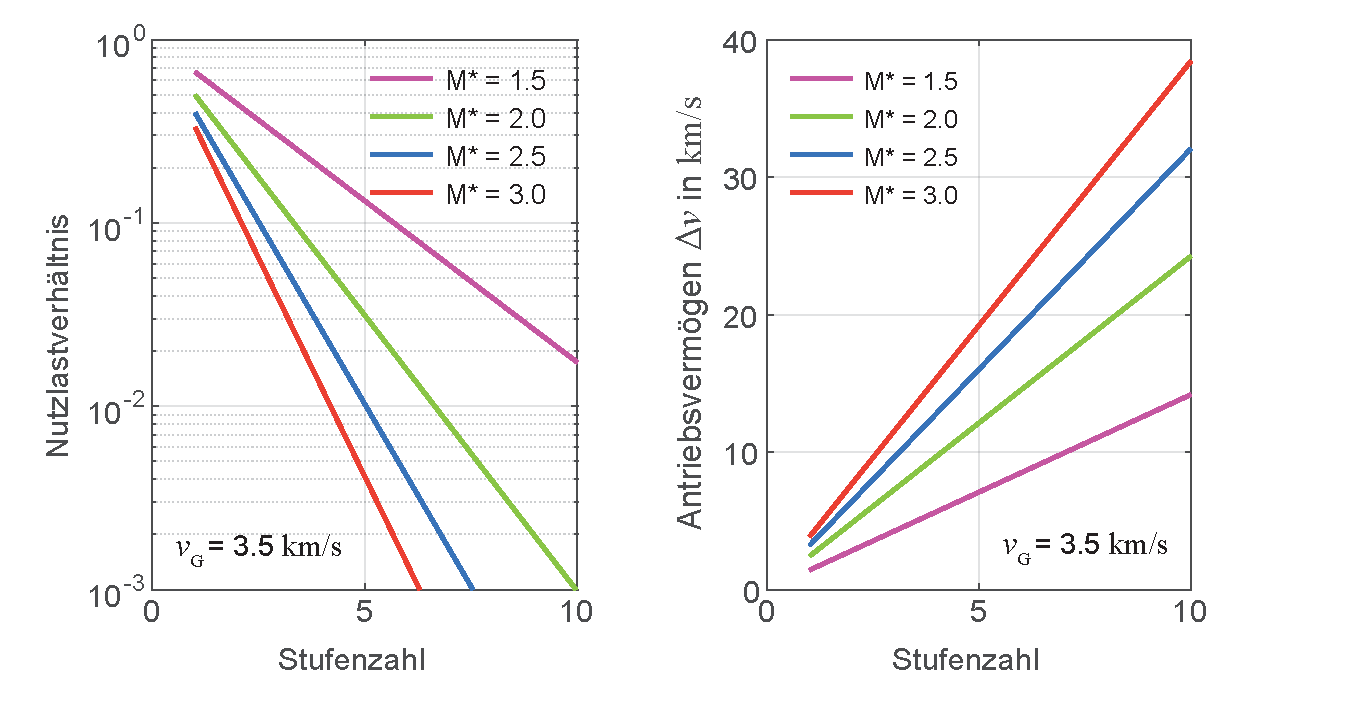
\includegraphics[width=\textwidth]{MehrStufenTheorie.pdf} 
	\caption[Nutzlastverh�ltnis �ber Antriebsbudget f�r mehrstufige Raketen.]{Nutzlastverh�ltnis �ber Antriebsbudget f�r mehrstufige Raketen bei gleichen $v_{\text{G},i}= v_\text{G}{}^*$ und 
	gleichen Struktur- und Treibstoffmassen aller Unterraketen ($\mathcal{M}^* = m_{0,i}/(m_{0,i}-m_{\text{T},i})$). Siehe \matlab{}-Datei
\mladynref{Raketenstart04.m}.}
	\label{abb:adyn_rocket_lsg05}
\end{figure}

\end{sol} 
\textcolor{blue} {$\rightarrow$ zur} \probref{adyn_rocketbasic}.\\
\noindent\rule[1ex]{\textwidth}{0.5pt}  \newpage  \clearpage

%-----------------------------------------------------------------------------------------------------------


\begin{sol}{prob:adyn_rocketopt1}\label{lsg:adyn_rocketopt1} %�bung3
\textbf{Optimierung Mehrstufenrakete (Tandemstufung)}\\
\begin{enumerate}
	\item \textit{\textbf{L�sungsansatz �ber Extremwertberechnung - Beispiel Saturn V Maximalleistung 100 t Nutzlast}}\\ 
Wir starten von der Raketen-Gleichung f�r die Tandemstufung \eqref{eq:adyn_rockets19} und fordern, dass f�r ein Nutzlastverh�ltnis
\begin{align}
    \Delta v = \sum\limits_{i_1}^N \Delta v_i = \sum\limits_{i_1}^N v_{\text{G},i}\,\ln\,\frac{1}{\sigma_i + \frac{\mu_{i+1}}{\mu_i}}\,.\label{eq:adyn_rocketsopt01} ~~~~ \rightarrow ~~~~ \text{max}
\end{align}
gelten soll. Die Bedingung f�r das Maximum lautet, wenn $\mu_\text{L}$ und alle $\sigma_i$ gegeben sind:
\begin{align}
    \frac{\d \Delta v\lk\mu_2,\mu_3,\ldots,\mu_N\rk}{\d \mu_i} = 0 ~~~~ \text{f�r} ~~~~i= 2,3,\ldots,N\,.\label{eq:adyn_rocketsopt02}
\end{align}
Daraus folgt sofort:
\begin{align}
    \frac{\d}{\d\mu_i}\,\lek -v_{\text{G},i-1}\,\ln\lk\sigma_{i-1} + \frac{\mu_i}{\mu_{i-1}}\rk- v_{\text{G},i}\,\lk\sigma_i + \frac{\mu_{i+1}}{\mu_i}\rk\rek= 0\,.\label{eq:adyn_rocketsopt03}
\end{align}
Wir f�hren  die Ableitung aus und erhalten $N-1$ Gleichungen in $\mu_i$ der Form: ($i=2,3,\ldots,N$)
\begin{align}
    \mu_i{}^2 = \frac{\lk v_{\text{G},i}-v_{\text{G},i-1}\rk\,\mu_{i+1}}{v_{\text{G},i-1}\,\sigma_i}\,\mu_i-\frac{v_{\text{G},i}}{v_{\text{G},i-1}}\,\frac{\sigma_{i-1}}{\sigma_i}\,\mu_{i-1}\,\mu_{i+1} = 0 \,,\label{eq:adyn_rocketsopt04}
\end{align}
\bzw aufgel�st nach
\begin{align}
    \mu_i = Q_i\,\mu_{i+1}+\sqrt{\lk Q_i\,\mu_{i+1}\rk^2 + P_i\,\mu_{i+1}\,\mu_{i-1}}\label{eq:adyn_rocketsopt05}
\end{align}
mit 
\begin{subequations}
\begin{align}
    Q_i = \frac{v_{\text{G},i}-v_{\text{G},i-1}}{2\,v_{\text{G},i-1}\,\sigma_i} \label{eq:adyn_rocketsopt06a}
\end{align}
und
\begin{align}
    P_i = \frac{v_{\text{G},i}\,\sigma_{i-1}}{v_{\text{G},i-1}\,\sigma_i}\;. \label{eq:adyn_rocketsopt06b}
\end{align}
\end{subequations}
F�r eine zweistufige Rakete ist $N=2$ und damit gibt es nur eine Bestimmungsgleichung f�r $\mu_2$ (da $\mu_1=1$ und $\mu_3 = \mu_L$):
\begin{align}
    \mu_2 = Q_2\,\mu_\text{L} + \sqrt{\lk Q_2\,\mu_\text{L}\rk^2 + P_2\,\mu_\text{L}}\,. \label{eq:adyn_rocketsopt07}
\end{align}
F�r eine dreistufige Rakete  ($N=3$) gibt es zwei Bestimmungsgleichungen
\begin{subequations}
\begin{align}
    \mu_2 &=  Q_2\,\mu_3 + \sqrt{\lk Q_2\,\mu_3\rk^2 + P_2\,\mu_3}\,, \label{eq:adyn_rocketsopt08a}\\
    \mu_3 &= Q_3\,\mu_\text{L} + \sqrt{\lk Q_3\,\mu_\text{L}\rk^2 + P_3\,\mu_\text{L}\,\mu_2}\,, \label{eq:adyn_rocketsopt08b}
\end{align}
\end{subequations}
die man am besten numerisch in \matlab{}  nach $\mu_2$ und $\mu_3$ l�st (siehe \mscr{} \mladynref{RaketenOptimierung01.m}). F�r $N=3$ f�hrt das Gleichungssystem 
nach einiger Algebra auf eine noch analytisch l�sbare kubische Gleichung f�r $\mu_3$, die wir hier angeben:
\begin{align*}
    \mu_3^3 - B\,\mu_3^2 + C\,\mu_3 - D &= 0 \\
		\text{mit}~~ B &= 2\mu_\text{L}\,(2Q_3+ Q_2\,P_3)\,,\\
		             C &= 4Q_3\,\mu\text{L}^2\,(Q_3+Q_2\,P_3)\,,\\
								 D &= P_2\,P_3{}^2\, \mu\text{L}^2\,.
\end{align*}
In \figref{adyn_optrockets01}a haben wir die Massenverh�ltnisse $\mu_2,\,\mu_3$ der einzelnen Raketenstufen f�r den Fall einer zweistufigen und einer dreistufigen Rakete �ber dem Nutzlastverh�ltnis aufgetragen. In \figref{adyn_optrockets01}b ist das mit heutigen Werten f�r $v_\text{G}$ maximal erzielbare Antriebsverm�gen f�r eine Stufenzahl von $N=2$ und $N=3$ �ber das Nutzlastverh�ltnis aufgetragen. Man erkennt daraus, dass man mit einer zweistufigen Rakete nicht zum Mond kommt, da $\Delta v$ kleiner als die 2.\,\gls{vkosmos} ist. \\

\begin{figure}[H]
	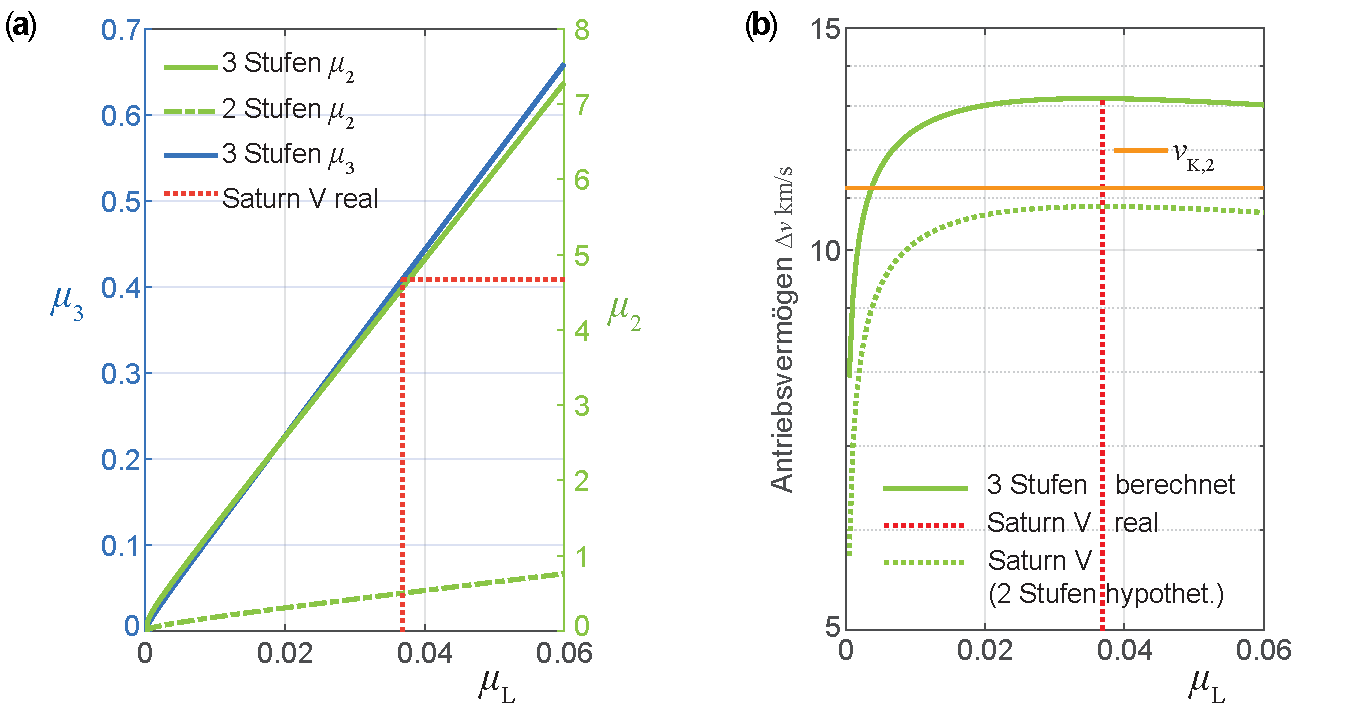
\includegraphics[width=\textwidth]{RaketenOptimierung01.pdf} 
	\caption[Optimierung einer Dreistufen-Rakete.]{Optimierung einer Dreistufen-Rakete. L�sung �ber Extremwertberechnung. \fa Berechnung der Massenverh�ltnisse der einzelnen Raketenstufen \fb Antriebsverm�gen f�r eine Dreistufen-Rakete (berechnet) und f�r die Saturn V. Zum Vergleich sind auch die Werte f�r eine (hypothetische) Ausf�hrung der Saturn V als Zweistufen-Rakete gezeigt.}
	\label{abb:adyn_optrockets01}
\end{figure}

\item \textit{\textbf{L�sungsansatz �ber Lagrange-Multiplikatoren - Beispiel Saturn V zum Mond}}\\ 
	
	Gegeben seien nach Aufgabenstellung: $v_{\text{G},i}$ (Ausstr�mgeschwindigkeit), $\sigma_i$ (Strukturparameter) und $m_0$ (Gesamtmasse der Rakete) \\
Variiert werden k�nnen die Massenverh�ltnisse $\mu_i$ oder, was gleichbedeutend ist, die Teil-Nutzlastverh�ltnisse $\eta_i$, die wir �ber
\begin{align}
    \eta_i = \frac{m_{\text{L},i}}{m_{0,i}-m_{0,i+1}} = \frac{m_{0,i+1}}{m_{\text{S},i} + m_{\text{T},i}} \label{adyn_optrocket11}
\end{align}
definieren. \\
Als $i$-tes Nutzlastverh�ltnis wird die Masse der n�chsten $\lk i+1\rk$-ten Unterrakete im Verh�ltnis zur Summe von Struktur- und Treibstoffmasse der $i$-ten Stufe definiert. Die Zahl der Stufen k�nnte ebenfalls variiert werden, soll aber hier festgehalten werden. \\
Zu optimieren/maximieren sind das Gesamt-Nutzlastverh�ltnis $\mu_\text{L}$ und das Gesamt-Antriebsverm�gen $\Delta v$, also max $\mu_\text{L}\lk \Delta v\rk$ \bzw max $\Delta v\lk\mu_\text{L}\rk $.\\
In Kapitel �ber den Lagrange-Formalismus im Band I hatten wir die Methode der Lagrange-Multiplikatoren kennen gelernt, mit der man die Extremwertberechnung der Wirkung $S$ bei Vorliegen von Zwangsbedingungen \bzw Nebenbedingungen durchf�hren konnte. Wir wenden dies f�r unser Problem an. Der Wirkung $S$ entspricht hier die Gr��e $\mu_\text{L}$ \bzw $\Delta v$, die Nebenbedingungen sind duch die $m_{\text{S},i}$ \bzw $\sigma_{i}$ gegeben und die "`Bewegungsgleichungen"' ergeben sich dann durch:
\begin{align}
    \frac{\d\lk\mu_\text{L}\rk}{\d \eta_j} + \lambda_{\mu_\text{L}}\,\frac{\d\lk \Delta v\rk}{\d \eta_j} = 0 ~~~~ \text{(maximieren von $\mu_\text{L}$)} \label{adyn_optrocket12}
\end{align}
\bzw
\begin{align}
    \frac{\d\lk\Delta v\rk}{\d \eta_j} + \lambda_{\Delta v}\,\frac{\d\lk \mu_\text{L}\rk}{\d \eta_j} = 0 ~~~~ \text{(maximieren von $\Delta v$)} \,.\label{adyn_optrocket13}
\end{align}
F�r $\lambda_{\mu_\text{L}} = 1/\lambda_{\Delta v}$ beschreiben beide Gleichungen das gleiche mathematische Problem.\\
Wir f�hren die Ableitungen aus und erhalten:
\begin{align}
\begin{split}
     \frac{\d\lk\Delta v\rk}{\d \eta_j} &= -v_{\text{G,j}}\,\frac{1-\sigma_j}{1+\eta_j}\,\frac{1}{\sigma_j+\eta_j} \,,\\
     \frac{\d\lk\mu_\text{L}\rk}{\d \eta_j}  &= \frac{\mu_\text{L}}{\eta_j\lk 1+\eta_j\rk}
\end{split}\label{adyn_optrocket14}
\end{align}
und erhalten aus \eqref{adyn_optrocket12}
\begin{align}
    \frac{\mu_\text{L}}{\eta_j\lk 1+\eta_j\rk} = \lambda_{\mu_\text{L}}\,v_{\text{G},j}\,\frac{1-\sigma_j}{1+\eta_j}\,\frac{1}{\sigma_j + \eta_j} \label{adyn_optrocket15} \,.
\end{align}
Daraus folgt sofort
\begin{align}
    v_{\text{G},j}\,\eta_j\,\frac{1-\sigma_j}{\sigma_j + \eta_j} = \frac{\mu_\text{L}}{\lambda_{\mu_\text{L}}} =:\gamma = \text{const} ~~~~ j=1,2,\ldots,N \,.\label{adyn_optrocket16}
\end{align}
Damit haben wir die Grundgleichungen f�r die Optimierung. \\
$\gamma$ ist noch eine unbekannte Gr��e, die es aus \eqref{adyn_optrocket16} zu bestimmen gilt. Wir nehmen diese zun�chst als bestimmt an, so dass sich dann die optimalen Nutzlastverh�ltnisse ergeben zu:
\begin{align}
    \eta_\text{j,\text{opt}} = \frac{\gamma\,\sigma_j}{\lk 1-\sigma_j\rk\,v_{\text{G},j}-\gamma}~~~~ j=1,2,\ldots,N \,.\label{adyn_optrocket17}
\end{align}
Wir setzen diese in die Raketen-Gleichung f�r die serielle Stufung \eqref{eq:adyn_rockets17} ein und erhalten:
\begin{align}
    \Delta v = \sum\limits_{j=1}^N\,v_{\text{G},j}\,\ln\,\frac{1+\eta_j}{\sigma_j + \eta_j} = \sum\limits_{j=1}^Nv_{\text{G},j}\,\ln\,\frac{v_{\text{G},j}-\gamma}{\sigma_j\,v_{\text{G},j}}\,.\label{adyn_optrocket18}
\end{align}
F�r das totale Nutzlastverh�ltnis 
\begin{align}
    \mu_\text{L} = \frac{m_\text{L}}{m_0} = \prod\limits_{j=1}^N\frac{\eta_j}{1+\eta_j} = \prod\limits_{j=1}^N \frac{\gamma\,\sigma_j}{\lk 1-\sigma_j\rk\lk v_{\text{G},j}-\gamma\rk}\,.\label{adyn_optrocket19}
\end{align}
Der weitere Weg besteht darin, dass man aus \eqref{adyn_optrocket18} f�r bekannte $\sigma_j$, $\Delta v$ die Konstante $\gamma$ (die aus dem Lagrange-Multiplikator abgeleitet wurde) bestimmt und diese in \eqref{adyn_optrocket19} einsetzt, um $\mu_\text{L,opt}$ zu erhalten. \\
Die Konstante $\gamma$ muss aus der Gleichung \eqref{adyn_optrocket16} numerisch bestimmt werden, was wir vorteilhaft in \matlab\,im Skript \mladynref{RaketenOptimierung02.m} ausgef�hrt haben.\\
Wenn wir die in der �bung in Tabelle \ref{tab:adyn_parameter_Apollo11} angegebenen Werte verwenden, erhalten wir aus der Rechnung einen Wert von $\mu_\text{L} = 0.0176$, der nur wenig von dem tats�chlichen (etwas kleineren) Wert von $\mu_\text{L} = 0.0162$ abweicht, mit dem die NASA (vermutlich aus Sicherheitsgr�nden) operierte.
In \figref{adyn_optrockets02} ist das maximale Nutzlastverh�ltnis gezeigt, mit der eine Nutzlast von $m_\text{L} = \mu_\text{L,opt}\cdot m_0$ auf ein bestimmtes Antriebsverm�gen gebracht werden kann.\\
Es sei noch darauf hingewiesen, dass $\gamma < \mathrm{min}\lk v_{\text{G},j}\,\lk 1-\sigma_j\rk \rk \,$f�r alle $j=1,\ldots,N$ sein muss, was bei der numerischen Berechnung zu ber�cksichtigen ist.
	
\begin{figure}[H]
	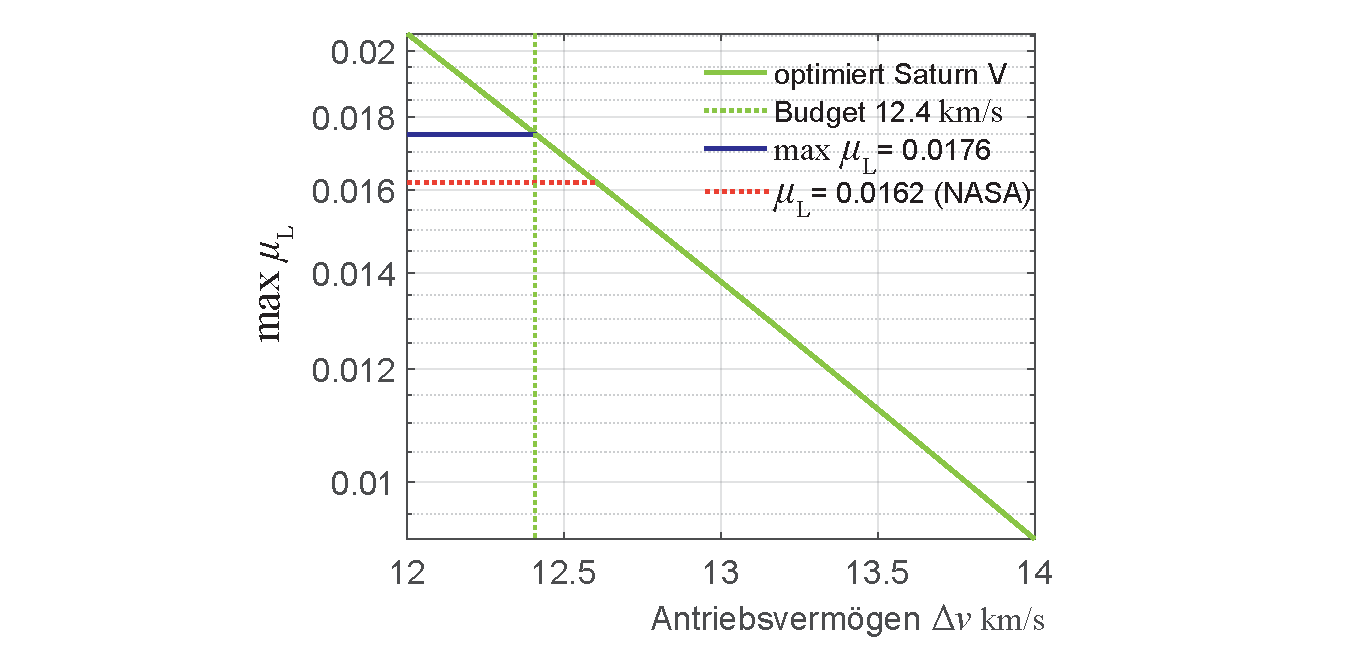
\includegraphics[width=\textwidth]{RaketenOptimierung02.pdf} 
	\caption[Optimierung einer Dreistufen-Rakete.]{Optimierung Saturn V Konfiguration f�r die Apollo Missionen. L�sung �ber Methode der Lagrange-Multiplikatoren. Berechnung des optimalen Antriebsverm�gens/Nutzlastverh�ltnisses.}
	\label{abb:adyn_optrockets02}
\end{figure}


\end{enumerate}

\end{sol} 
\textcolor{blue} {$\rightarrow$ zur} \probref{adyn_rocketopt1}.\\
\noindent\rule[1ex]{\textwidth}{0.5pt}  \newpage  \clearpage


%-----------------------------------------------------------------------------------------------------------


\begin{sol}{prob:adyn_rocketopt2}\label{lsg:adyn_rocketopt2} %�bung4
\textbf{Vergleich Mehrstufenrakete (Serielle und Parallelstufung)} \\ \\
Wir fassen die Vor- und Nachteile der Tandemstufung gegen�ber der Parallelstufung  in der folgenden Tabelle zusammen.\\
\begin{table}%tab1
\caption{Vor- und Nachteile der Tandemstufung gegen�ber der Parallelstufung.}
\smallskip
\hspace{1.5cm}
\begin{tabular}{L{3cm}L{3cm}L{3cm}}
\svhline\noalign{\smallskip}
Eigenschaft				    			& Tandemstufung				& Parallelstufung \\
\noalign{\smallskip}\svhline\noalign{\smallskip}
\noalign{\smallskip}
Startbeschleunigung							&kleiner &gr��er\\	
Strukturbelastung 							&kleiner &gr��er\\	
Biegemomente      							&gr��er  &kleiner\\	
Aerodynamische Verluste 				&kleiner &gr��er\\	
Gravitationsverluste						&gr��er  &kleiner\\	
Gesamtl�nge Rakete							&gr��er  &kleiner\\	
\noalign{\smallskip}
\svhline\noalign{\smallskip}
\end{tabular} \\
\label{tab:adyn_vergleich_staging}
\end{table}%tab1


\end{sol} 
\textcolor{blue} {$\rightarrow$ zur} \probref{adyn_rocketopt2}.\\
\noindent\rule[1ex]{\textwidth}{0.5pt}  \newpage  \clearpage


%-----------------------------------------------------------------------------------------------------------


%-----------------------------------------------------------------------------------------------------------
%-----------------------------------------------------------------------------------------------------------

\subsection{�bungen zu Umlaufbahnen}

\medskip

%-----------------------------------------------------------------------------------------------------------

\begin{sol}{prob:adyn_orbits1}\label{lsg:adyn_orbits1} %�bung5
\textbf{Bahnparameter aus Bodenbeobachtungen}\\ \\
\textit{Bahnparameter von Satelliten mit gegebenen geozentrischen Orts- und Geschwindigkeitsdaten:}\\ \\
Wir verwenden die Formeln aus \kap{adyn_orbits_determination_rv} und erhalten:\\

Satellit 1 (HEO)
\begin{align*}
	&\text{Halbachse}\,\,a & \SI{20251.57}{\km}\\
	&\text{Exzentrizit�t}\,\,e & 0.777596\\
	&\text{Bahnneigung} \,\,i &   10.194 \degree\\
	&\text{Knoten} \,\, \Omega &  171.951 \degree\\
	&\text{Arg. Perig�um} \,\, \omega &  86.081 \degree\\
	&\text{Mittl. Anomalie} \,\, M &  138.824  \degree\\
	&\text{Mittl. Bewegung} \,\, n & \SI{2.19e-04}{\per\second} \\
\end{align*}

Satellit 2 (LEO)
\begin{align*}
	&\text{Halbachse}\,\,a & \SI{8225.40}{\km}\\
	&\text{Exzentrizit�t}\,\,e & 0.076722\\
	&\text{Bahnneigung} \,\,i &   6.707 \degree\\
	&\text{Knoten} \,\, \Omega &  145.881 \degree\\
	&\text{Arg. Perig�um} \,\, \omega &  86.476 \degree\\
	&\text{Mittl. Anomalie} \,\, M &  167.278  \degree\\
	&\text{Mittl. Bewegung} \,\, n & \SI{8.46e-04}{\per\second}
\end{align*}

\newpage

\textit{Bahnparameter der ISS aus den ver�ffentlichten geozentrischen Orts- und Geschwindigkeitsdaten der NASA:}\\
	%\url{https://spotthestation.nasa.gov/trajectory_data.cfm}\\

Auch hier verwenden wir die Formeln aus \kap{adyn_orbits_determination_rv} und erhalten:
\begin{align*}
	&\text{Halbachse}\,\,a & \SI{6803.28}{\km}\\
	&\text{Bahnh�he}\,\,h & \SI{425.28}{\km}\\
	&\text{Exzentrizit�t}\,\,e & 0.001855\\
	&\text{Bahnneigung} \,\,i &  51.751 \degree\\
	&\text{Knoten} \,\, \Omega &  47.685 \degree\\
	&\text{Arg. Perig�um} \,\, \omega & 124.00 \degree\\
	&\text{Mittl. Anomalie} \,\, M & 315.75 \degree\\
	&\text{Umlaufzeit} \,\, n & \SI{93.8 }{\minute}
\end{align*}
Die mittlere Anomalie $M$ wurde so angepasst, dass der Anfangswert mit den NASA Daten �bereinstimmt. Wir verweisen auf \kap{adyn_orbits_determination_singulaer}
zur Berechnung alternativer Bahnparameter bei kreisf�rmigen und �quatorialen Bahnen, sowie auf die Zusatzaufgabe \probref{adyn_orbits_zusatz1}.
\begin{figure}[H]
	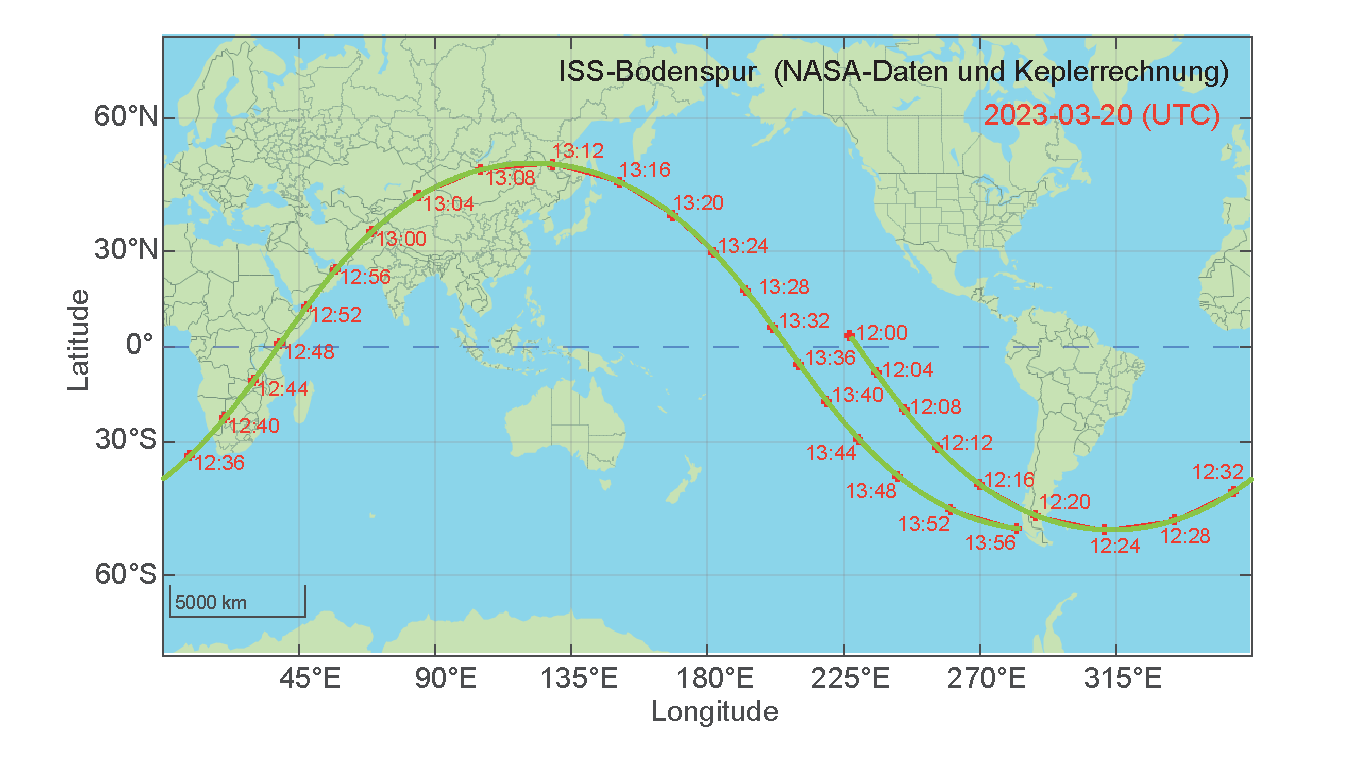
\includegraphics[width=\textwidth]{GroundTrackISS20032023.pdf} 
	\caption[Bodenspur der ISS.]{Bodenspur der ISS. Vergleich NASA Daten und Berechnung Keplerbahn.}
	\label{abb:adyn_satobserv02}
\end{figure}
Die Berechnungen finden sich im Detail im \mscr{} \mladynref{BahnparaBestimmung01.m}. 

\end{sol} 
\textcolor{blue} {$\rightarrow$ zur} \probref{adyn_orbits1}.\\
\noindent\rule[1ex]{\textwidth}{0.5pt}  \newpage  \clearpage

%-----------------------------------------------------------------------------------------------------------
\newpage

\begin{sol}{prob:adyn_orbits2}\label{lsg:adyn_orbits2} %�bung6
\textbf{Bodenspuren von Erdsatelliten}\\ 

\begin{itemize}
	\item \textit{\textbf{Bodenspuren verschiedener Satellitenarten}}\\
		\begin{itemize}
			\item Bodenspur eines GEO-Satelliten.
			\item Bodenspur eines Molnija-Satelliten (HEO-Satelliten).
			\item Bodenspur eines polaren Satelliten. 
		\end{itemize}
		\begin{figure}[H]
			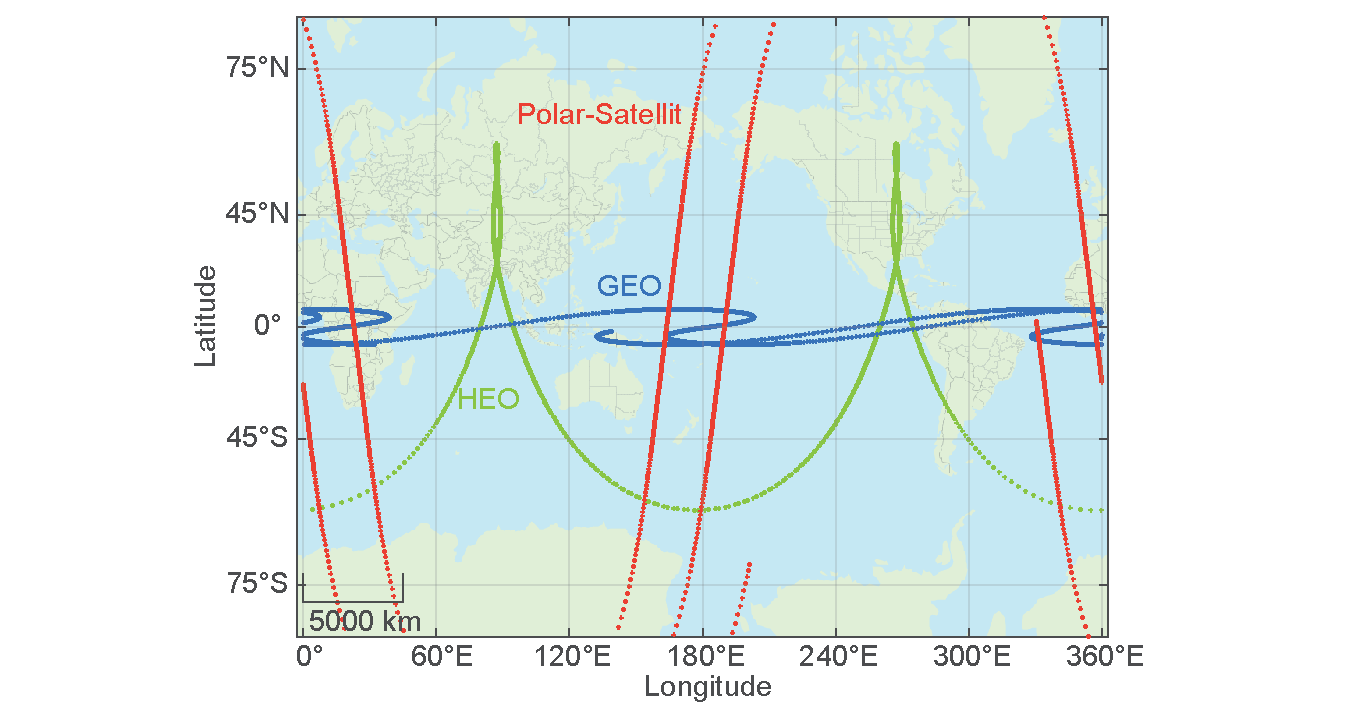
\includegraphics[width=0.9\textwidth]{Orbits03a.pdf} 
			\caption[Bodenspuren von verschiedenen Satelliten.]{Bodenspuren von verschiedenen Satelliten. GEO:\, $a = \SI{25000}{\km},\, e = 0.73,\, i = 8\degree,\, \Omega =45\degree$,\,\, HEO (Typ Molnija-Satelliten):\, $a = \SI{26555}{\km},\, e = 0.72,\, i = 63.4\degree,\, \Omega =120\degree,\,\omega =270\degree$,\,\, Polar-Satellit:\, $a = \SI{7330}{\km},\, e = 0.0,\, i = 93\degree,\, \Omega =130\degree,\,\omega =0\degree$.}
			\label{abb:adyn_orbits03a}
			\end{figure}
	\item \textit{\textbf{Bodenspuren verschiedener Satelliten in geosynchronen Umlaufbahnen}}\\

				Die Bodenspuren \figref{adyn_orbits03b} �hneln den verschiedenen Analemma, die wir im \kap{kulmination_sonne} \bzw in der \probref{hm_Analemma_Mars} kennen gelernt hatten. Das ist nicht verwunderlich. In einer geozentrischen Betrachtung �bernehmen die Satelliten die Rolle der Sonne, die unterschiedlichen Formen des \textit{\anf{Satelliten-Analemmas}} kommen durch die unterschiedlichen Bahnparameter zustande. Siehe auch im Detail \probref{hm_Analemma_Mars}.\\
\newpage
			\begin{figure}[H]
			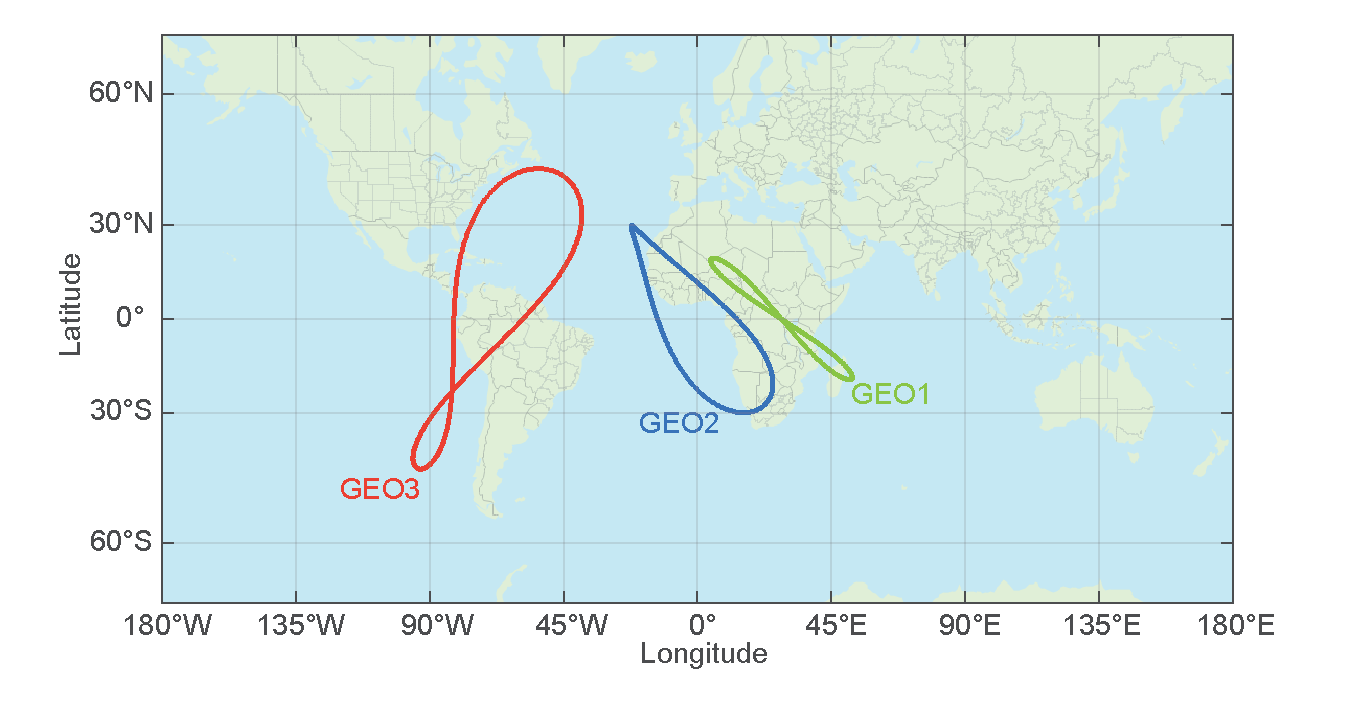
\includegraphics[width=0.95\textwidth]{Orbits03b.pdf} 
			\caption[Bodenspuren von verschiedenen geosynchronen Satelliten.]{Bodenspuren von verschiedenen geosynchronen Satelliten. Parameter siehe \probref{adyn_orbits2}.}
			\label{abb:adyn_orbits03b}
			\end{figure}
\item \textit{\textbf{Bodenspur ISS}}\\
			\begin{figure}[H]
			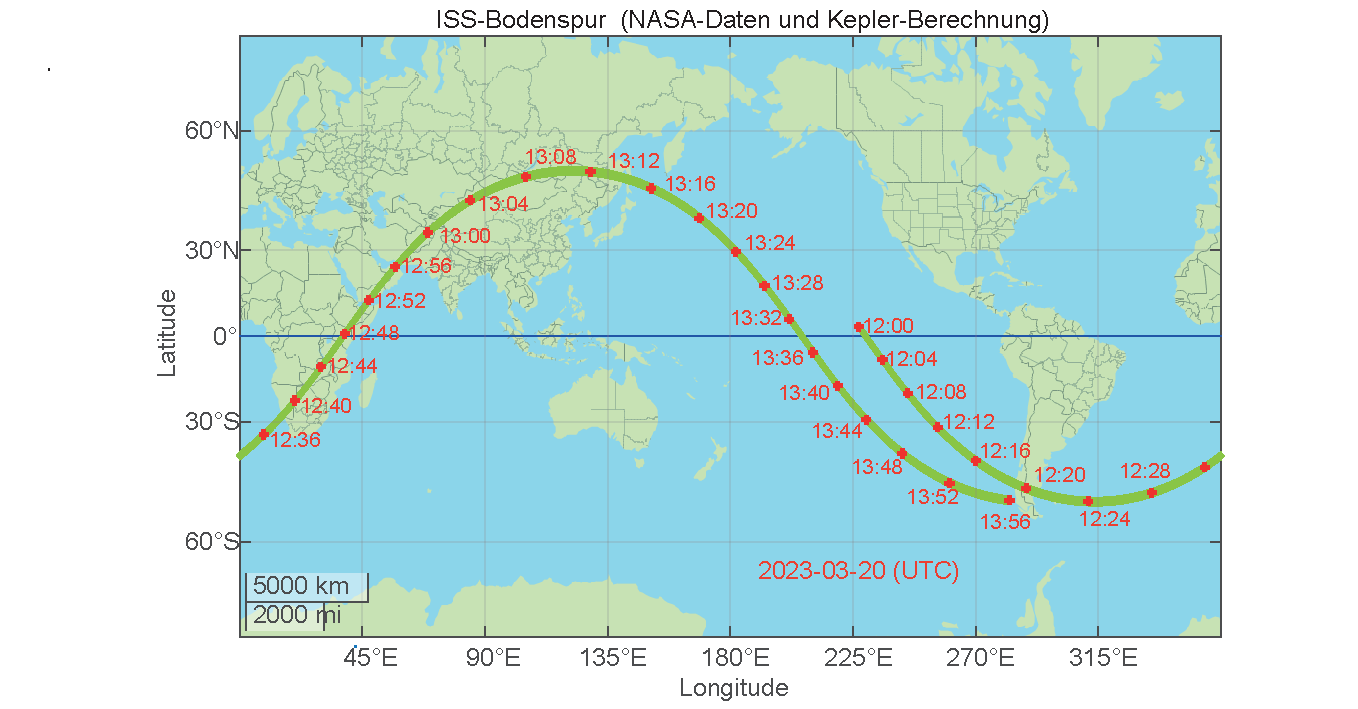
\includegraphics[width=0.95\textwidth]{ISSBodenspur.pdf} 
			\caption[Bodenspuren der ISS.]{Bodenspuren der ISS vom 20.03.2023. Parameter siehe \probref{adyn_orbits2}.}
			\label{abb:adyn_orbits03c}
			\end{figure}
\end{itemize}
Die Berechnungen finden sich im Detail im \mscr~\mladynref{SatPositionen01.m} \bzw \mladynref{SatPositionen02.m}.

\end{sol} 
\textcolor{blue} {$\rightarrow$ zur} \probref{adyn_orbits2}.\\
\noindent\rule[1ex]{\textwidth}{0.5pt}  \newpage  \clearpage

%-----------------------------------------------------------------------------------------------------------

\begin{sol}{prob:adyn_orbits3}\label{lsg:adyn_orbits3} %�bung7
\textbf{Bodenbeobachtung von Erdsatelliten}\\ \\

Die Berechnungen finden sich im Detail im \mscr~\mladynref{SatPositionen03.m} \bzw \mladynref{SatPositionen04.m}.
\begin{figure}[H]
	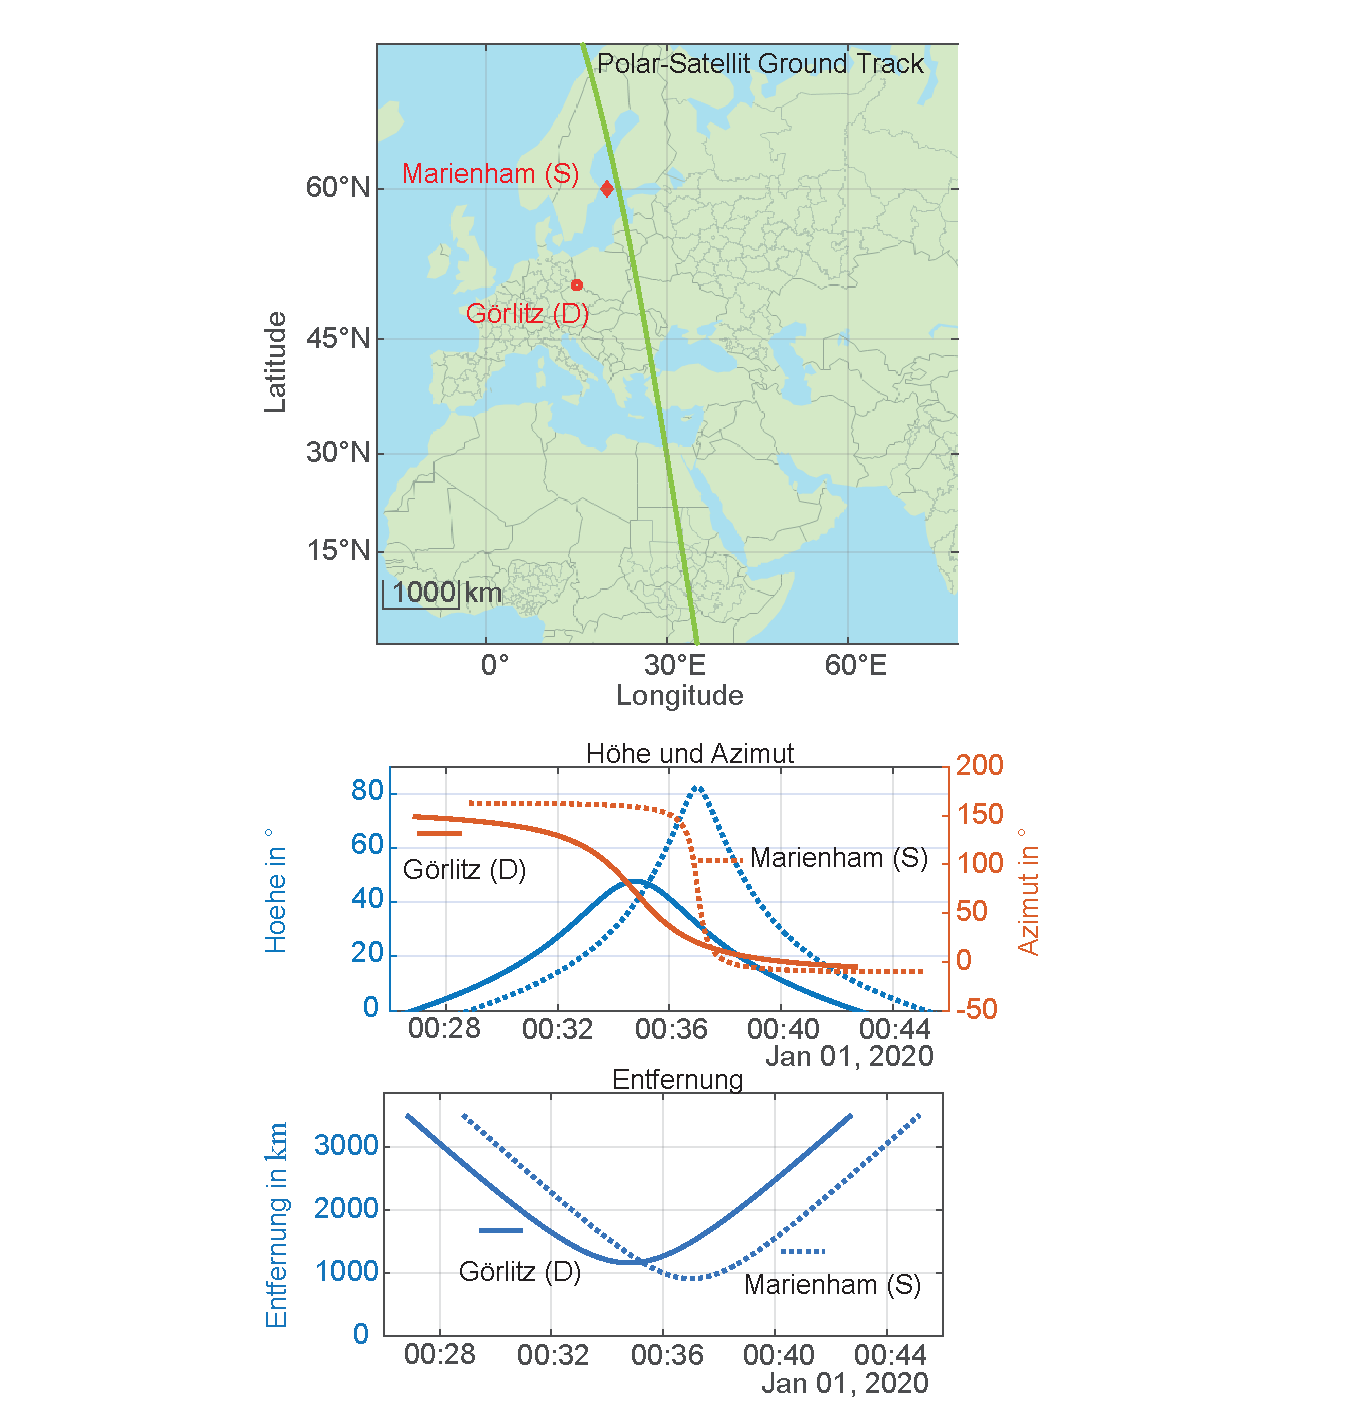
\includegraphics[width=\textwidth]{TopographPolarerSat.pdf} 
	\caption[Topographische Beobachtung eines polaren Satelliten.]{Bodenspur, Azimut, H�he und Entfernung eines polaren Satelliten von zwei Bodenstationen. Parameter siehe \probref{adyn_orbits3} und \mscr~\mladynref{SatPositionen03.m} \bzw \mscr~\mladynref{SatPositionen03a.m}.}
	\label{abb:adyn_satobserv03}
\end{figure}
\begin{figure}[H]
	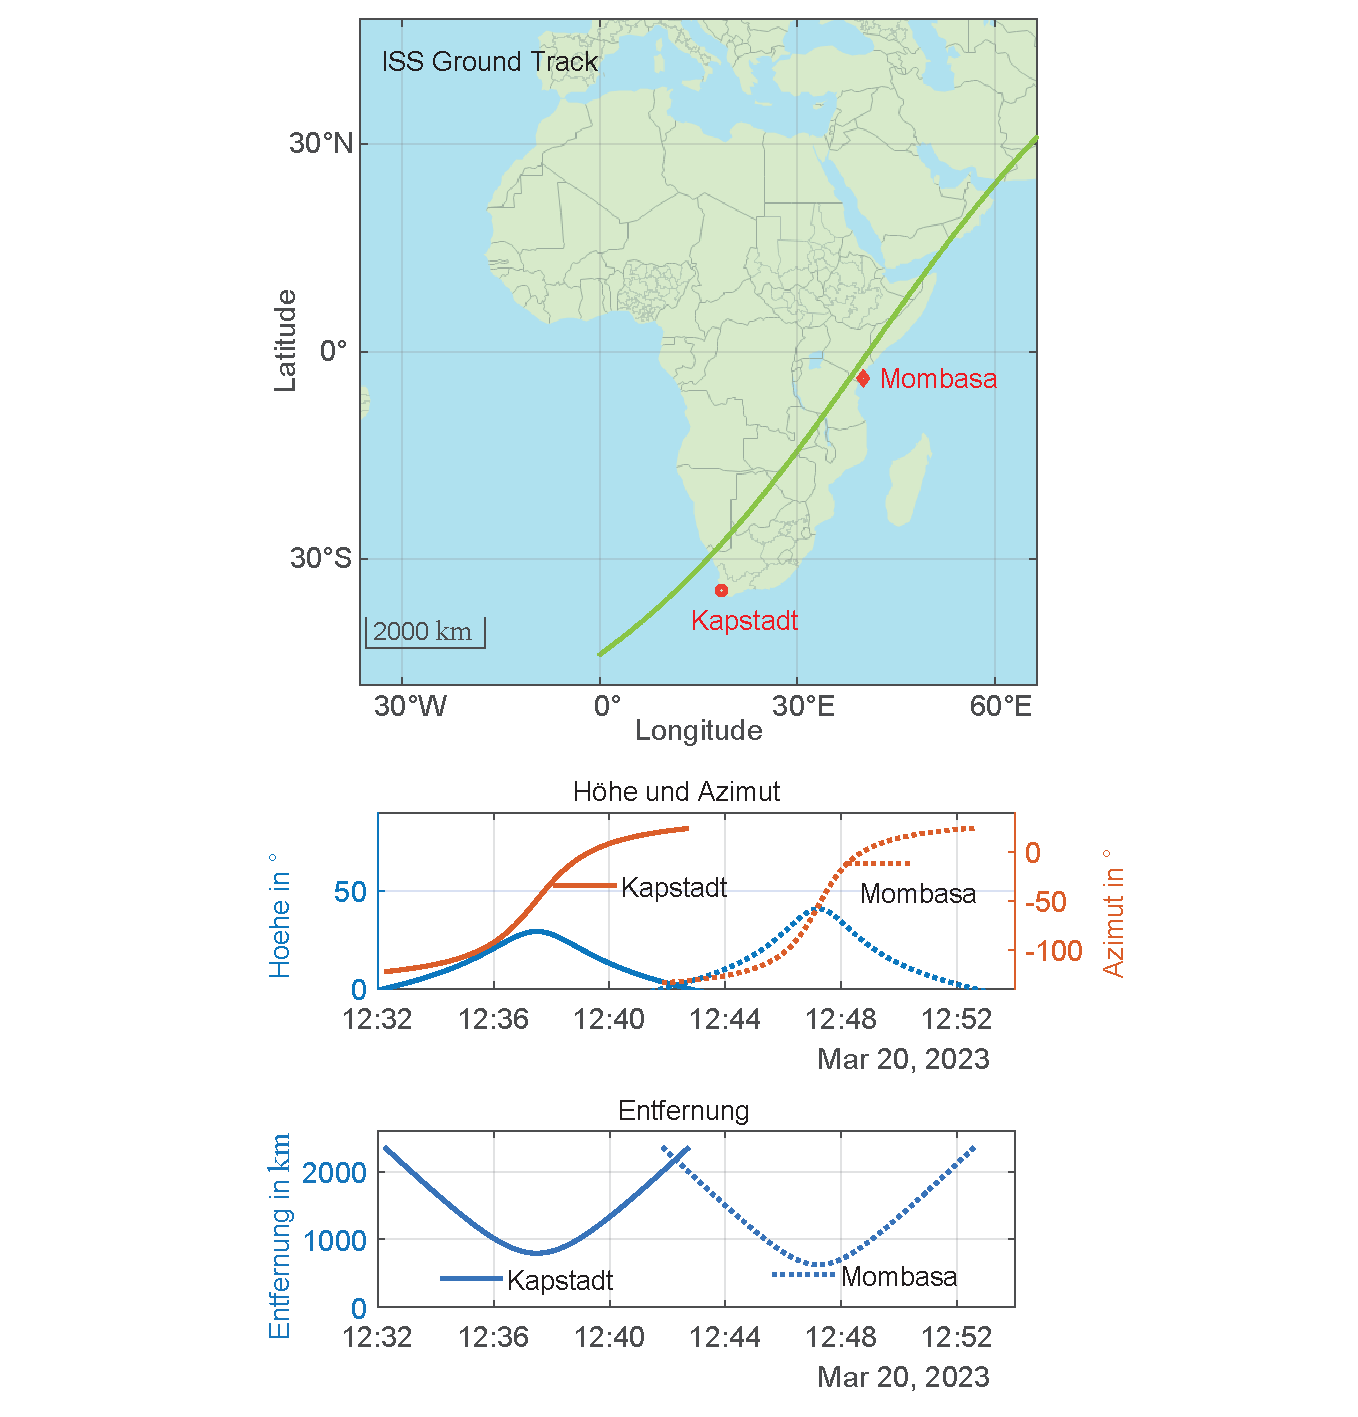
\includegraphics[width=\textwidth]{TopographISS.pdf} 
	\caption[Topographische Beobachtung der ISS.]{Bodenspur, Azimut, H�he und Entfernung der von zwei Bodenstationen. Parameter siehe \probref{adyn_orbits3} und \mscr~\mladynref{SatPositionen04.m}.}
	\label{abb:adyn_satobserv04}
\end{figure}

\end{sol} 
\textcolor{blue} {$\rightarrow$ zur} \probref{adyn_orbits3}.\\
\noindent\rule[1ex]{\textwidth}{0.5pt}  \newpage  \clearpage

%-----------------------------------------------------------------------------------------------------------

\begin{sol}{prob:adyn_orbits4}\label{lsg:adyn_orbits4} %�bung8
\textbf{Bodenbeobachtung eines Molniya-Satelliten}\\ \\

Die Berechnungen finden sich im Detail im \mscr~\mladynref{SatPositionen05.m}.
\begin{figure}[H]
	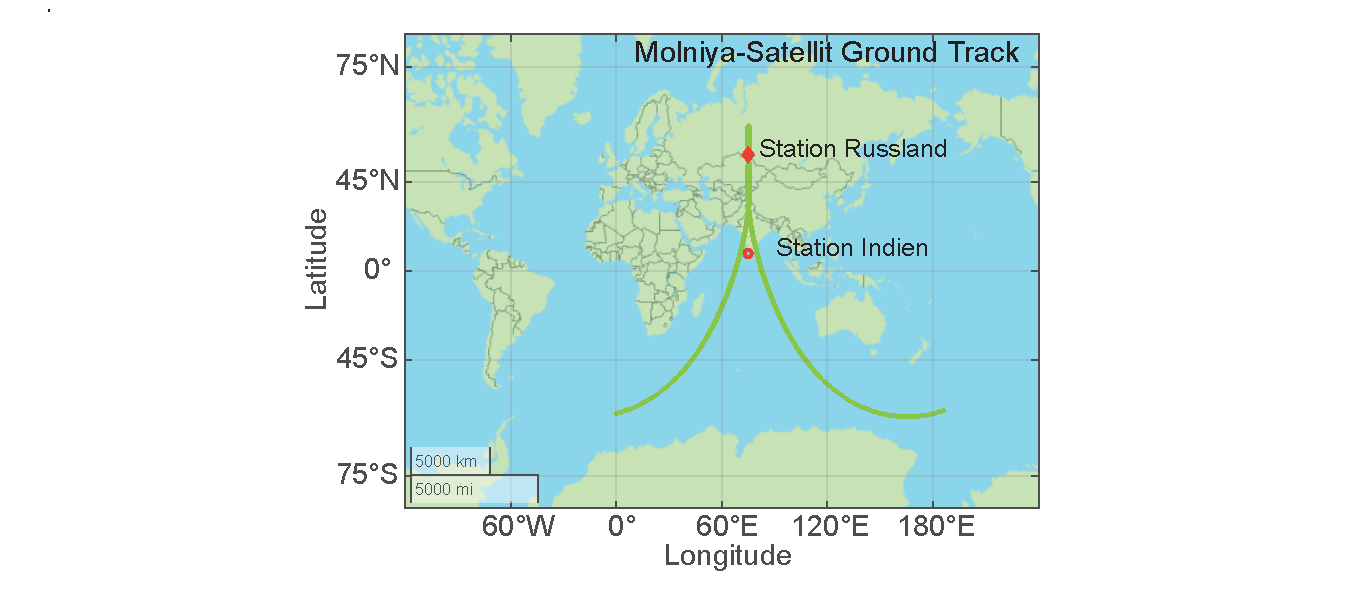
\includegraphics[width=\textwidth]{TopographMolniyaSat01.pdf} 
	\caption[Bodenspur eines Molniya-Satelliten.]{Bodenspur eines Molniya-Satelliten.\\Parameter siehe \probref{adyn_orbits4} und \mscr~\mladynref{SatPositionen05.m}.}
	\label{abb:adyn_MolniyaObserv01}
\end{figure}
\begin{figure}[H]
	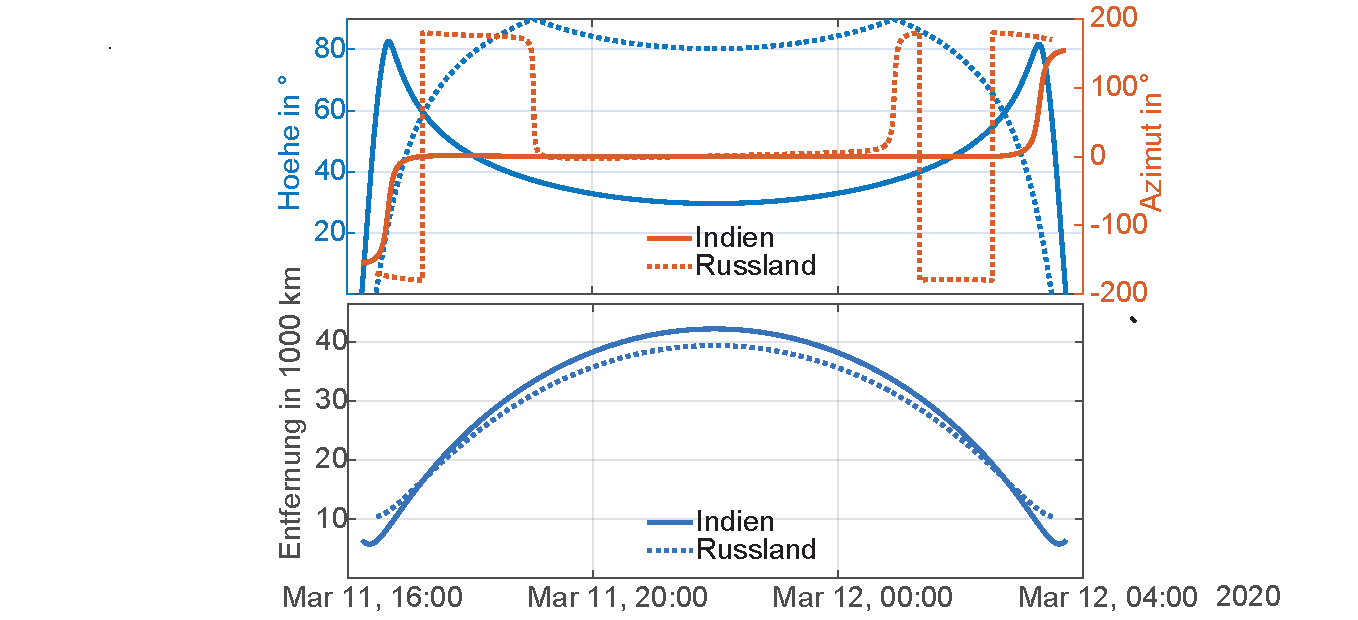
\includegraphics[width=\textwidth]{TopographMolniyaSat02.pdf} 
	\caption[Topographische Beobachtung eines Molniya-Satelliten.]{Azimut, H�he und Entfernung eines Molniya-Satelliten von zwei Bodenstationen. Parameter siehe \probref{adyn_orbits4} und \mscr~\mladynref{SatPositionen05.m}.}
	\label{abb:adyn_MolniyaObserv02}
\end{figure}
\end{sol} 
\textcolor{blue} {$\rightarrow$ zur} \probref{adyn_orbits4}.\\
\noindent\rule[1ex]{\textwidth}{0.5pt}  \newpage  \clearpage


%-----------------------------------------------------------------------------------------------------------

\begin{sol}{prob:adyn_orbits5}\label{lsg:adyn_orbits5} %�bung9
\textbf{Sonnensynchrone Bahnen}\\ \\

Die Drehimpulserhaltung gilt streng nur f�r das Zweik�rperproblem, dann ist auch die Bahnebene fest im Raum orientiert und die Bahn geschlossen.\\
Wie wir \zb in \kap{Periheldrehung} gesehen haben, bewirkt die Abplattung der Erde jedoch ein Drehmoment auf die Bahn und f�hrt zu einer Verschiebung der Rektaszension des aufsteigenden Knotens. 
Man kann mit Hilfe der St�rungsrechnung zeigen (siehe auch \probref{adyn_pertubations}), dass die Frequenz dieser Pr�zession des aufsteigenden Knoten sich nach folgender Formel berechnet:
	\begin{align}
		\dot{\Omega} = -\frac{3}{2} J_2\, \frac{2\pi}{T_\text{E}} \lk \frac{R_\text{E}}{a\,(1-e^2)} \rk^2 \cos i = 
		-\frac{3}{2} J_2\,R_\text{E}\, \sqrt{\frac{a_\text{E}}{a_\text{E}{}^2}} \, \frac{\cos i}{a^2\,(1-e^2)^2} = C\,f(a,e,i)\,. \label{eq:adyn_orbits5_01}
	\end{align}
Hierin sind $J_2$ die sogenannte zonale Harmonische\index{Harmonische!zonale} (siehe \kap{adyn_gravity_pertubations}) als Ma� f�r die Abplattung der Erde, $R_\text{E}$ der mittlere Erdradius, $a$ die gro�e Halbachse der Satellitenbahn und $i$ \bzw $e$ deren Neigung (Inklination) \bzw Exzentrizit�t. $T_\text{E} = 2\pi\sqrt{a_\text{E}{}^3/\mu_\text{E}}$ ist die Umlaufzeit der Erde um die Sonne.\footnote{Genauer gesagt ist es die Zeit eines anomalistischen Jahres ($\SI{365.25963}{}\,\mathrm{d}$, siehe \kap{hm_zeitdefinition})} Die Pr�zession ist umso gr��er, je geringer die Inklination $i$ und die Bahnh�he $a$ sind.\\
Wegen des Minuszeichen wirkt bei einer retrograden Bahnen (Bahn entgegen der Erdrotation, \dh $i > 90\degree$) diese Pr�zession in die gleiche Richtung wie die Erdrotation. Man kann also durch geeigneter Wahl von Inklination und Flugh�hen daf�r sorgen, dass sich die Bahn gerade um so viel verschiebt wie der mittleren Bewegung der Erde ($2\pi/T_\text{E}$) um die Sonne entspricht (\figref{adyn_synchron_orbit}). 

Bei einem SSO erfolgt der �berflug des Satelliten �ber einen Punkt auf der Oberfl�che des Planeten immer zur selben Ortszeit, vorausgesetzt die geographische Breite des Ortes liegt innerhalb des Bereiches, der durch die Inklination der Bahn begrenzt wird. Aufgrund dieser konstanten �berflugszeit lassen sich Beobachtungen von verschiedenen Tagen und Jahreszeiten gut miteinander vergleichen, deswegen haben ja Wetter- und Erdbeobachtungssatelliten oft solche Bahnen.

\begin{figure}[H]
	\includegraphics[width=\textwidth]{SonnensynchroneBahn.pdf} 
	\caption[Sonnensynchrone Bahn.]{Sonnensynchrone Bahn. Symbolische und nicht-ma�stabsgetreue Darstellung. }
	\label{abb:adyn_synchron_orbit}
\end{figure}

\newpage
\textbf{Zusatzaufgabe}\\

Wir wollen nun noch die Bodenspur des ERS-1 SSO-Satelliten berechnen \cite{Gottschalk1991}. Man k�nnte nun aus \eqref{eq:adyn_orbits5_01} einen der Parameter $a,\, e$ oder $i$ berechnen und die anderen vorgeben. 
Man hat aber eben mit $a$ einen weiteren Freiheitsgrad neben $i$, womit man auch fordern kann, dass die Bahnh�he $h$ so gew�hlt wird, dass ein �berflug �ber eine Gebiet (\zb das �berkreuzen des �quators nach $K$ Tagen \bzw. $N$ Orbits genau wiederholt (sogenannte \textit{Sonnensynchrone Repeat Orbits}).  Anfangs w�hlte man f�r den ERS-1 K=3, N=43, sp�ter ging man auf K=35.
Um das zu erreichen, muss man auch die St�rungen der Perihelverschiebung (siehe \kap{Stoerpotential_Merkur}) und der mittleren Anomalie ber�cksichtigen. Diese sind f�r kreisf�rmige Bahnen gegeben durch \cite{Montenbruck2012, Murray2008, Vallado2007}:

	\begin{align}
	\begin{split}
		\dot{\omega} = -\frac{3}{4} J_2\, n_0 \frac{R_\text{E}{}^2}{a^2} \lk 1 - 5\cos^2 i\rk \\ 
    \Delta n = n - n0  = -\frac{3}{4} J_2\, n_0 \frac{R_\text{E}{}^2}{a^2} \lk 1 - 2\cos^2 i\rk\,,
	\end{split}\label{eq:adyn_orbits5_02}
\end{align}

worin $n_0=\sqrt{(GM_\text{E}/a^3)}$ die mittlere Bewegung der Kepler-Bahn ist.
F�r sonnensynchrone Bahnen ist dann gefordert, dass gilt:

	\begin{align}
		\dot{\Omega} - \dot{\theta} = -360\degree\,, \\ 
\label{eq:adyn_orbits5_03}
\end{align}

woraus man f�r die Umlaufzeit einer solchen Bahn die Beziehung

	\begin{align}
		T_\text{P,SSO} = \frac{2\pi}{n_0-\Delta n-\dot{\omega}}\,, \\ 
\label{eq:adyn_orbits5_04}
\end{align}

was etwas l�nger ist als die Umlaufzeit im reinen Kepler-Fall.
Durch Iteration mit dem Startwert $T_\text{P,SSO}^{(0)}= 2\pi/n_0$ findet man �ber \eqref{eq:adyn_orbits5_02} aus \eqref{eq:adyn_orbits5_01} nacheinander $a$ und $i$ f�r die geforderten Bedingungen.\\

Wir finden:
\begin{align} 
  h &= a - R_\text{E} = \SI{7153.1}{\km} - \SI{6371.0}{\km} = \SI{782.1}{\km}\,, \\
	i &= 98.5\degree,
\end{align}
was f�r unsere Kreisbahnn�herung gut mit den Werten in \cite{Gottschalk1991} �bereinstimmt.
F�r die Berechnung der Bodenspur zu verschiedenen Zeiten, m�ssen Sie die Zeitabh�ngigkeit von $\Omega(t) = \Omega(t_0) + \dot{\Omega}\,(t-t_0)$ beachten.\\
Die Rechnungen finden sich im Detail im \mscr~\mladynref{SonnenSynchroneBahn.m} und ein Ergebnis in \figref{adyn_synchron_groundtrack}.

\begin{figure}[H]
	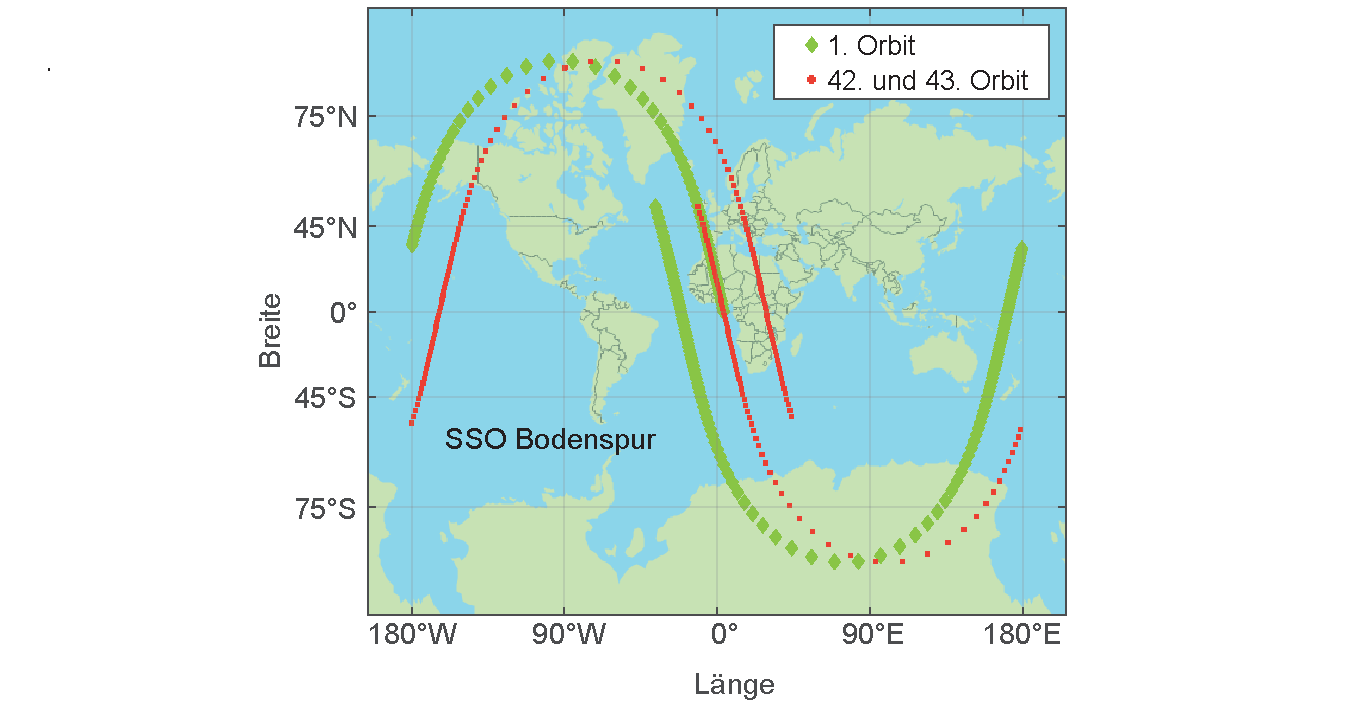
\includegraphics[width=\textwidth]{SonnensynchroneBodenspur.pdf} 
	\caption[Sonnensynchroner \textit{Repeat Orbit} -Bodenspur.]{Sonnensynchroner \textit{Repeat Orbit} - Bodenspur. Gezeigt sind Orbit Nr. 1 (willk�rlich gew�hlt) und die Orbits Nr 42 und Nr. 43 als Bodenspur. Man sieht, dass bei $N=43$ nach 3 Tagen der Satellit genau �ber die gleichen Gebiete fliegt wie beim Orbit $N=1$.}
	\label{abb:adyn_synchron_groundtrack}
\end{figure}

Wir empfehlen auch die Zusatz�bung \probref{adyn_pertubations}.

\end{sol} 
\textcolor{blue} {$\rightarrow$ zur} \probref{adyn_orbits5}.\\
\noindent\rule[1ex]{\textwidth}{0.5pt}  \newpage  \clearpage


%-----------------------------------------------------------------------------------------------------------

\begin{sol}{prob:adyn_starlink}\label{lsg:adyn_starlink} %�bung10
\textbf{Starlink}
\begin{figure}[H]
	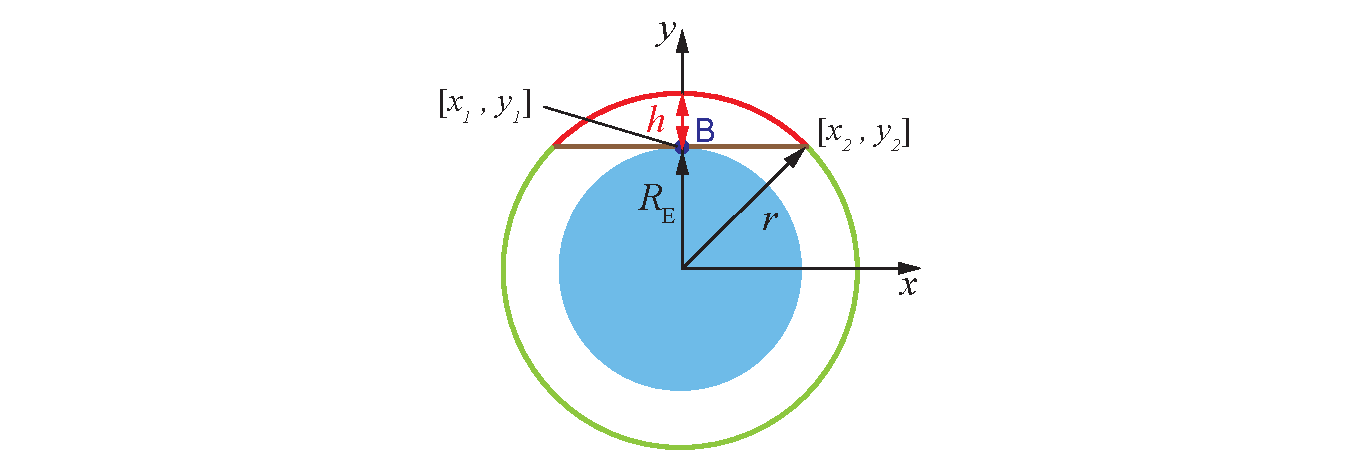
\includegraphics[width=\textwidth]{StarlinkGeometrie.pdf} 
	\caption[Zur Geometrie der Starlink-Beobachtungen.]{[Zur Geometrie der Starlink-Beobachtungen. Mit rot ist die Kugelkappe dargestellt die ein Beobachter auf der Erde sieht, wenn sich ein Starlink-Satellit in einer Kugelschale mit Radius $R_\text{E} + h$ bewegt.}
	\label{abb:adyn_starlink_ueb01}
\end{figure}
\begin{enumerate}
\item [1)] Wir berechnen zun�chst den Anteil $\gamma\lk h\rk$ der Kugelschale mit Radius $R_\text{E} + h$, den ein Beobachter von der Erdoberfl�che aus sieht. \\
    Nach \figref{adyn_starlink_ueb01} ist das:
    \begin{align*}
        \gamma\lk h\rk = \frac{A_\text{KK}}{A_\text{K}} \,. 
    \end{align*}
    Hierin ist $A_\text{K}$ ist die Oberfl�che einer Kugel $4\pi\,r^2 = 4\pi\,\lk R_\text{E} +h\rk^2$ und $A_\text{KK}$ die Oberfl�che der Kugelkappe, die man sich leicht �ber 
    \begin{align*}
       A_\text{KK} &= 2\pi\,r\int\limits_{x_1}^{x_2} y(x)\,\sqrt{1+y'(x){}^2}\D x = 2\pi\int\limits_{\rho_1}^{\rho_2} y(\rho)\,\sqrt{1+y'(\rho){}^2}\,\D \rho 
    \end{align*}
    mit $y = \sqrt{r^2-x^2}$,\,  $1+y'{}^2 = r^2/(r^2-x^2)$,\, $r = R_\text{E} + h$\, und \,$x= \rho\,\cos\phi$ herleiten kann.\\
		Somit erh�lt man 
    \begin{align}
		  A_\text{KK} &= 2\pi\,r \int\limits_{R_\text{E}}^{R_\text{E} + h}\,\D \rho = 2\pi\,\lk R_\text{E} +h\rk \,h \nonumber \\
      \rightarrow~~~  \gamma\lk h\rk &= \frac{2\pi\,\killA{\lk R_\text{E} + h\rk}\,h}{4\pi\,\lk R_\text{E} + h\rk^\killA{2}} = \frac{1}{2}\,\frac{h}{R_\text{E} + h} \,. \label{eq:adyn_starlink_ueb01}
    \end{align}
    Mit den Angaben aus der Aufgabenstellung sind damit jederzeit pro Schale $n_i $ Satelliten 
    \begin{align*}
        n_i = \gamma\lk n_i\rk \cdot \,N_i = 
        \begin{cases} 
        190 \\ 
        63\\
        223
        \end{cases}
    \end{align*}
    und insgesamt $n_\text{ges} = \sum n_i \approx 476$ Satelliten zu sehen.
\newpage
\item [2)] Wir nehmen eine Gleichverteilung der Satelliten in der Kugelschale an. Dann ergibt sich f�r einen Beobachter eine Raumwinkeldichte von
    \begin{align}
        \Omega_\text{ges} = \frac{n_\text{ges}}{2 \pi} \approx 75.8 \,. \label{eq:adyn_starlink_ueb03}
    \end{align}
    Der Nenner von $2\pi$ (anstelle $4\pi$) ergibt sich, aus der Tatsache, dass wir bereits in der Berechnung von \eqref{eq:adyn_starlink_ueb01} ber�cksichtigt hatten, dass der Beobachter nur den Halbraum sieht. Wir rechnen den Raumwinkel auf Quadratgrad ($\square^\degree$) um:
    \begin{align*}
        4\pi^2 = \lk 2\pi\rk^2 \widehat{=} \lk 360^\degree\rk^2 = 129600\,\square^\degree \,.
    \end{align*}
    und erhalten damit aus \eqref{eq:adyn_starlink_ueb03}
    \begin{align}
        \Omega_\text{ges} = \frac{n_\text{ges}}{2\pi} \approx 0.023\,\frac{1}{\square^\degree} \,.\label{eq:adyn_starlink_ueb04}
    \end{align}
    Umgekehrt hei�t das, dass f�r eine Kantenl�nge $d_\square$ eines Winkelquadrats am Himmel von 
    \begin{align}
        d_\square = \sqrt{A_\square} = \frac{1}{\sqrt{\Omega_\text{ges}}} \approx 6.6\degree   \label{eq:adyn_starlink_ueb05}
    \end{align}
    in etwa ein Starlink-Satellit zu sehen ist. \\
    Die Winkelgeschwindigkeit eines Starlink-Satelliten ist nach dem Keplerschen Gesetz durch
    \begin{align*}
        \omega_i = \sqrt{\frac{G\,M_\text{E}}{\lk R_\text{E} +h_i\rk^3}} = 
        \begin{cases} 
        \SI{3.95}{\degree\per\minute} \\ 
        \SI{3.75}{\degree\per\minute}\\
        \SI{3.3}{\degree\per\minute}
        \end{cases} \,.
    \end{align*}
    Der Mond hat einen Winkeldurchmesser von \ca $\SI{0.5}{\degree}$, \dh ein Starlink-Satellit \anf{durchquert} den Mond in weniger als $\Delta t = 0.5/\omega_i \approx \SI{8}{\second}$.
\end{enumerate}

\end{sol} 
\textcolor{blue} {$\rightarrow$ zur} \probref{adyn_orbits5}.\\
\noindent\rule[1ex]{\textwidth}{0.5pt}  \newpage  \clearpage





%-----------------------------------------------------------------------------------------------------------


\subsection{�bungen zu Man�vern im Weltall}

\medskip

%-----------------------------------------------------------------------------------------------------------

\begin{sol}{prob:adyn_rocket_analogy}\label{lsg:adyn_rocket_analogy} %�bung11
\textbf{Analogie zum Oberth-Effekt\index{Oberth-Effekt}}\\

Zun�chst k�nnte man denken, es spielt keine Rolle, wo die Rakete gez�ndet wird. Dem ist aber nicht so.\\
Wir betrachten den Gewinn an kinetischer Energie des Raketenautos durch den kurzen Raketenimpuls ($m_0$ ist die Masse der Rakete ohne Treibstoff) im festen KOS $\sum$:
\begin{align}
\begin{split}
    \Delta T_\text{R} &=\frac{1}{2}\,m_0\,\lk v+\Delta v\rk^2 - \frac{1}{2}\,m_0\,v^2\\
    &= \frac{1}{2}\,m_0\,\lk\Delta v\rk^2 - m_0\,v\,\Delta v  \,. 
\end{split}\label{eq:adyn_rocket_analogy01}
\end{align}
Der Gewinn an kinetischer Energie h�ngt interessanterweise von $v$ ab.\\
Der Impuls der gez�ndeten Rakete auf das Raketenauto ist aber unabh�ngig von $v$:
\begin{align}
    m_0\,\Delta v = m_\text{G}\,v_\text{G} = F\,\Delta t\,, \label{eq:adyn_rocket_analogy02}
\end{align}
worin $m_\text{G}$, $v_\text{G}$ die Masse \bzw die Geschwindigkeit des ausgesto�enen Treibgases sind, $F$ der Schub und $\Delta t$ ein kleines Zeitintervall. \\
Die Bezeichnung Ausstr�mgeschwindigkeit des Treibgases verdient eine genauere Betrachtung, es ist n�mlich die Geschwindigkeit des Gases relativ gemessen zum Schwerpunkt des Systems Raketenauto und Treibstoff. \\
Wie kann man das Paradoxon erkl�ren? Indem man die Ver�nderung der kinetischen Energie des Treibstoffs (\bzw der ausstr�menden Gase) wiederum im festen KOS $\sum$ betrachtet: 
\begin{align}
\begin{split}
    \Delta T_\text{G} &=\frac{1}{2}\,m_\text{G}\,\lk v_\text{G}-v\rk^2 - \frac{1}{2}\,m_\text{G}\,v^2\\
    &= \frac{1}{2}\,m_\text{G}\,v_\text{G}{}^2 - m_\text{G}\,v_\text{G}\,\Delta v \,.
\end{split} \label{eq:adyn_rocket_analogy03}
\end{align}
Man betrachte, dass hier in die Beziehung die Relativgeschwindigkeit $|v_\text{G} - v|$ eingeht, da im festen KOS sich ja der Treibstoff vor dem Z�nden bereits mit $v$ bewegt (\figref{adyn_rocket_analogy02}).\\

\begin{figure}[H]
	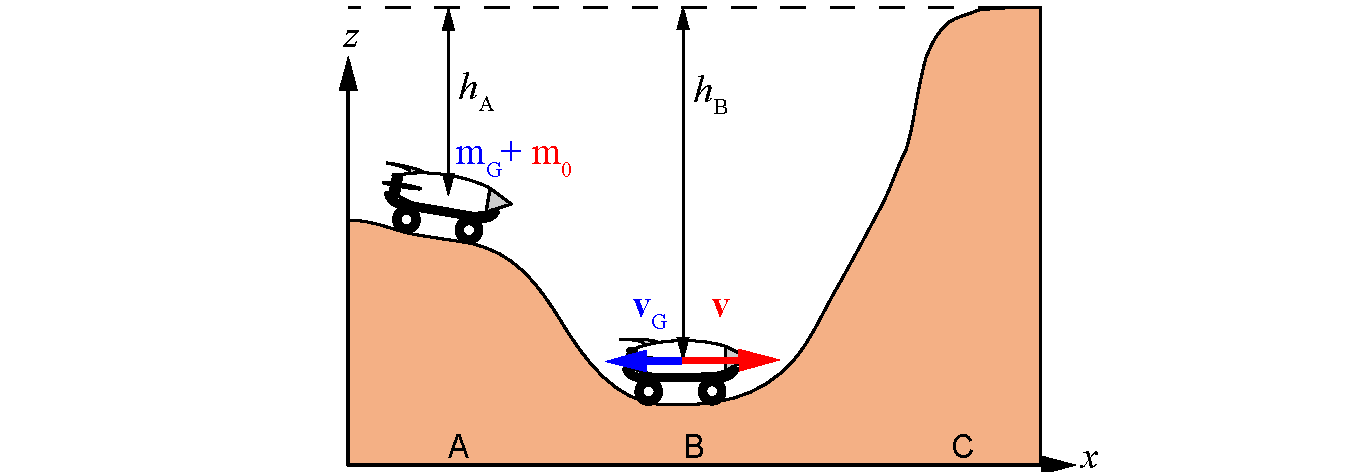
\includegraphics[width=\textwidth]{OberthEffAnalogie.pdf} 
	\caption[Analogie-Modell zum Oberth-Effekt.]{Analogie-Modell zum Oberth-Effekt.}
	\label{abb:adyn_rocket_analogy02}
\end{figure}

Die gesamte Ver�nderung der kinetischen Energie vom Raketenauto und Treibstoff muss gleich der freigesetzten chemischen Energie des Treibstoffs $\Delta E_\text{T}$ sein:
\begin{align}
\begin{split}
    \Delta T &= \Delta T_\text{R} + \Delta T_\text{G} \\
    &=\frac{1}{2}\,m_\text{G}\,v_\text{G}{}^2 + \frac{1}{2}\,m_0\lk\Delta v\rk^2 + \underbrace{m_0\,v\,\Delta v - m_\text{G}\,v\,v_\text{G}}_{\text{wegen \eqref{eq:adyn_rocket_analogy02}} =0} \\
    \Delta T &= \frac{1}{2}\,m_\text{G}\,v_\text{G}{}^2 + \frac{1}{2}\,m_0\lk\Delta v\rk^2 = \Delta E_\text{T}\,. 
\end{split} \label{eq:adyn_rocket_analogy04}
\end{align}
Die gesamte kinetische Energie ist wie erwartet unabh�ngig von $v$ und wegen der Energieerhaltung gleich $\Delta E_\text{T}$. \\

Was bedeutet das nun f�r den Z�ndungszeitpunkt? Wir untersuchen zwei Zeitpunkte (\bzw Orte) $A$ und $B$. 
Es gilt f�r die Gesamtenergien vor dem Z�nden:
\begin{align*}
    E_\text{A} &= -\lk m_0+ m_\text{G}\rk\,g\,h_\text{A}  \,,\\
    E_\text{B} &= -\lk m_0 + m_\text{G} \rk\,g\,h_\text{B} + T_\text{B} \\
    &= -\lk m_0+m_\text{G}\rk\,g\,h_\text{B}  + \frac{1}{2}\lk m_\text{G} +m_0\rk\,v_\text{B}{}^2 = -\lk m_0 + m_\text{G} \rk\,g\,h_\text{A}     \,.
\end{align*}
Aus $E_\text{A} = E_\text{B}$ folgt $v_\text{B} = \sqrt{2g\lk h_\text{B} -h_\text{A}\rk }$.\\

Unmittelbar nach dem Z�nden am Punkt $B$ gilt:
\begin{align*}
    E_\text{R}' =\,&\frac{1}{2}\,m_0\lk v_\text{B}+\Delta v\rk^2 - m_0\,g\,h_\text{B} + \frac{1}{2}\,m_\text{G}\lk v_\text{B} -v_\text{G}\rk^2 - m_\text{G}\,g\,h_\text{B}\\
    = \,&\frac{1}{2}\,m_0\lk\Delta v\rk^2 + m_0\,g\,h_\text{A} -m_0\,\Delta v\,\sqrt{2g\lk h_\text{B}-h_\text{A}\rk} \,,\\
		E_\text{G}' = \,& \frac{1}{2}\,m_\text{G}\,v_\text{G}{}^2 -m_\text{G}\,g\,h_\text{A} - m_\text{G}\,v_\text{G}\,\sqrt{2g\lk h_\text{B}-h_\text{A}\rk} \,,\\
    E_\text{ges}' = \,&\frac{1}{2}\,m_0\,\lk\Delta v\rk^2 + \frac{1}{2}\,m_\text{G}\,v_\text{G}{}^2 - \lk m_0 + m_\text{G}\rk\,g\,h_\text{A} = \, E_\text{A} + \Delta E_\text{T} \,.
\end{align*}
Man erkennt, dass die Energie der Rakete einen von $\sqrt{\lk h_\text{B} -h_\text{A}\rk}$ abh�ngigen Term hat, der offensichtlich verschwindet, wenn $h_\text{B} = h_\text{A}$ ist, es also keine Potentialmulde gibt. \\
Wir bestimmen jetzt noch wie gro� $\Delta v$ sein mu�, um den Punkt C zu erreichen, wenn die Rakete bei $B$ gez�ndet wird. 
\begin{align}
\begin{split}
    \frac{1}{2}\,m_0\,v_\text{C}{}^2 &= \frac{1}{2}\,m_0\,\lk \Delta v\rk^2 - m_0\,g\,h_\text{A} +m_0\,\Delta v \,\sqrt{2g\lk h_\text{B}-h_\text{A}\rk}\\
    \rightarrow ~~~~ 0 &= \lk \Delta v\rk^2 + 2\,\Delta v\,\sqrt{2g\lk h_\text{B}-h_\text{A}\rk} - 2\,g\,h_\text{A}\\
    \rightarrow ~~~~ \lk \Delta v\rk_\text{min} &= \sqrt{2g\lk h_\text{B}-h_\text{A}\rk} + \sqrt{\frac{g}{2}\,\lk h_\text{B}-h_\text{A}\rk + 2\,g\,h_\text{A}} 
\end{split}\,.\label{eq:adyn_rocket_analogy06}
\end{align}
Wie erwartet wird $\Delta v$ f�r $h_\text{B} = h_\text{A}$ zu $\Delta v= \sqrt{2\,g\,h_\text{A}}$. \\
Wir haben $\Delta v\lk h_\text{B}, h_\text{A}\rk$ in \figref{adyn_rocket_analogy03} dargestellt.\\

Die Analogie zum Oberth-Effekt der Raumfahrt ist offensichtlich. Wenn man den gr��tm�glichen beschleunigenden Effekt auf ein Raumschiff haben will, startet man das Man�ver am Punkt der Bahn, wo die Geschwindigkeit am gr��ten ist, \dh im Perig�um oder allgemein an der Periapsis. \\
Einfach gesprochen besagt der Oberth-Effekt, dass ein Raumschiff bei einem Impulsman�ver etwas Energie zus�tzlich zur chemischen Energie des Treibstoffs  \anf{stehlen} kann und zwar von der urspr�nglichen kinetischen Energie, die der Treibstoff vor dem Z�nden auf Grund der Bewegung der Rakete hatte. Anders gesagt: Der Schub generiert einen Impuls proportional zu $\Delta v$. Da die Energie proportional zu $v^2$ ist, ist dieser generierte Impuls energetisch um so wirksamer, je gr��er die Geschwindigkeit $v$ zu Beginn des Schubs ist.


\begin{figure}[H]
	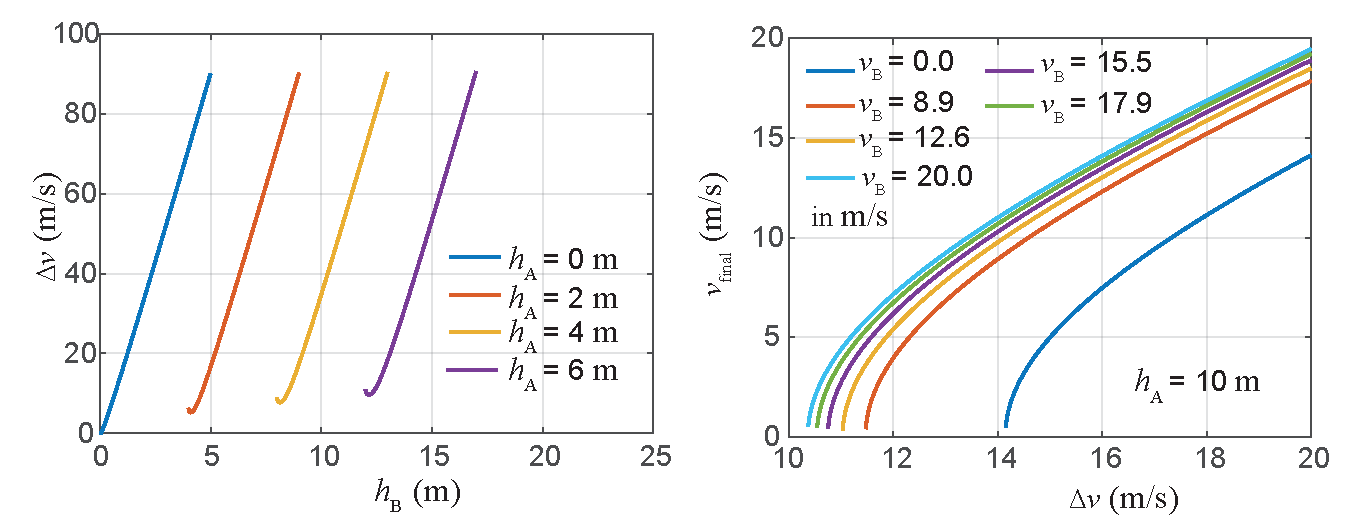
\includegraphics[width=\textwidth]{OberthEffAnalogie02.pdf} 
	\caption[Antriebsbedarf eines Raketenautos durch eine Potentialmulde.]{Antriebsbedarf eines Raketenautos durch eine Potentialmulde als Analogie-Modell zum Oberth-Effekt (Parameter siehe \mscr~\mladynref{OberthEffektAnalogie.m}).}
	\label{abb:adyn_rocket_analogy03}
\end{figure}

\end{sol} 
\textcolor{blue} {$\rightarrow$ zur} \probref{adyn_rocket_analogy}.\\
\noindent\rule[1ex]{\textwidth}{0.5pt}  \newpage  \clearpage


%-----------------------------------------------------------------------------------------------------------

\begin{sol}{prob:adyn_manoevers1}\label{lsg:adyn_manoevers1} %�bung12
\textbf{Hohmann-Transfer}
\begin{itemize}
   \item �bergangszeit f�r den Hohmann-Transfer als Funktion von $r_2/r_1$ \\
	Die �bergangszeit ergibt sich als halbe Umlaufzeit f�r die Hohmann-Ellipse:
	\begin{align*}
    t_\text{H} = \pi\sqrt{\frac{a_\text{H}{}^3}{m_\text{ZK}\,G}} = \frac{\pi}{\sqrt{m_\text{ZK}\,G}}\,\sqrt{\lk \frac{r_1+r_2}{2}\rk^3}\,.
\end{align*}
F�r den Fall eines Hohmann-Transfers von der Erdbahn in den interplanetaren Raum sind die Zeiten in \figref{adyn_Hohmann_TOF} dargestellt (\mscr~\mladynref{HohmannTransfer.m}).
\begin{figure}[H]
	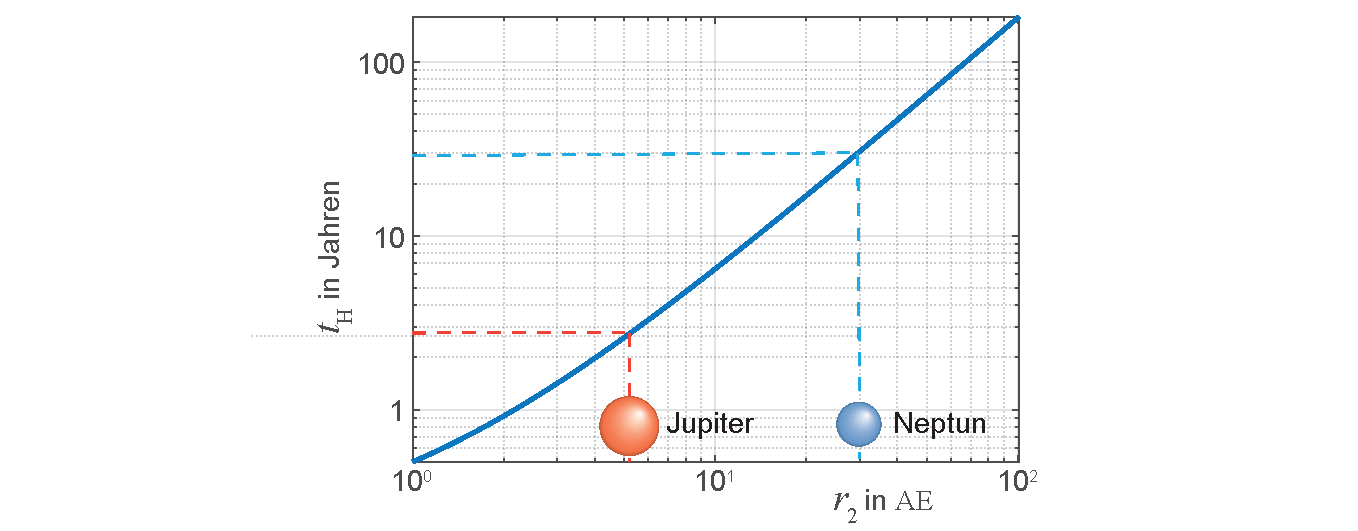
\includegraphics[width=\textwidth]{HohmannTOF.pdf} 
	\caption[Hohmann-Transferzeiten.]{Hohmann-Transferzeiten.}
	\label{abb:adyn_Hohmann_TOF}
\end{figure}
   \item $\Delta v$ gr��er als die \gls{vescape}\\
	F�r $r_2 \rightarrow \infty$ geht $\Delta v_2 \rightarrow 0$ und $\Delta v_1 \rightarrow v_\text{F}$. Daher ist in einem Bereich von $3.3 < r_2/r_1 < \infty$ die Summe $\Delta v_1+\Delta v_2$ gr��er als $v_\text{F}$, wie man leicht aus \eqref{eq:adyn_hohmann04} zusammen mit \eqref{eq:adyn_hohmann03a} und  \eqref{eq:adyn_hohmann03b} herleiten kann.\\
	Im Allgemeinen braucht man insgesamt mehr Antriebsenergie wenn eine Raumsonde erst impulsiv beschleunigt wird, dann durch Gravitation verlangsamt wird und anschlie�end wieder beschleunigt wird, als wenn die gesamte Antriebsimpuls in der Form von $\Delta v_1 = v_\text{F}$ aufgebracht wird.\\
   \item Hohmann-Transfer f�r Verringerung des Bahnradius\\
	Beim Hohmann-�bergang von h�heren auf niedrigere Bahnen gelten die Formeln unver�ndert, der Antriebsbedarf ist negativ und als Schub gegen die Flugrichtung zu verstehen.\\
\end{itemize}

\end{sol} 
\textcolor{blue} {$\rightarrow$ zur} \probref{adyn_manoevers1}.\\
\noindent\rule[1ex]{\textwidth}{0.5pt}  \newpage  \clearpage

%-----------------------------------------------------------------------------------------------------------
\begin{sol}{prob:adyn_manoevers2}\label{lsg:adyn_manoevers2} %�bung13
\textbf{Bielliptischer �bergang}\\

Zwei-Impuls-�bergang von Bahn mit Radius $r_1$ auf eine elliptische Bahn mit Radius $r_2$: 
F�r den Hohmann-Transfer nach $\infty$ ($r_2 \to\infty)$ k�nnen wir schreiben:
\begin{align*}
    \Delta v_1 = \sqrt{\frac{\mu}{r_1}}\,\lk \sqrt{2}-1\rk = v_1\lk \sqrt{2}-1\rk\,.
\end{align*}
Hierin ist $\mu$ der Gravitationsparameter f�r den jeweiligen betrachteten Zentrlk�rper (Erde, Sonne). Analog folgt in der umgekehrten Richtung (aus dem $\infty$ auf die Kreisbahn $r_2$):
\begin{align*}
    \Delta v_2 = v_2 \lk \sqrt{2}-1 \rk
\end{align*}
und somit mit $ \gamma = r_2 / r_1$:
\begin{align*}
    \frac{\Delta v_2}{v_1} = \frac{v_2}{v_1}\,\lk \sqrt{2}-1\rk = \sqrt{\frac{r_1}{r_2}} \,\lk\sqrt{2}-1\rk = \frac{\sqrt{2}-1}{\sqrt{\gamma}}\,.
\end{align*}
Der Gesamt-Antriebsbedarf ist dann: 
\begin{align*}
    \frac{\Delta v}{v_1} = \frac{\Delta v_1+\Delta v_2}{v_1} = \frac{\Delta v_1}{v_1}+\frac{\Delta v_2}{v_1} = \lk \sqrt{2} -1\rk\lk 1 + \frac{1}{\sqrt{\gamma}}\rk\,.
\end{align*}
\begin{figure}[H]
	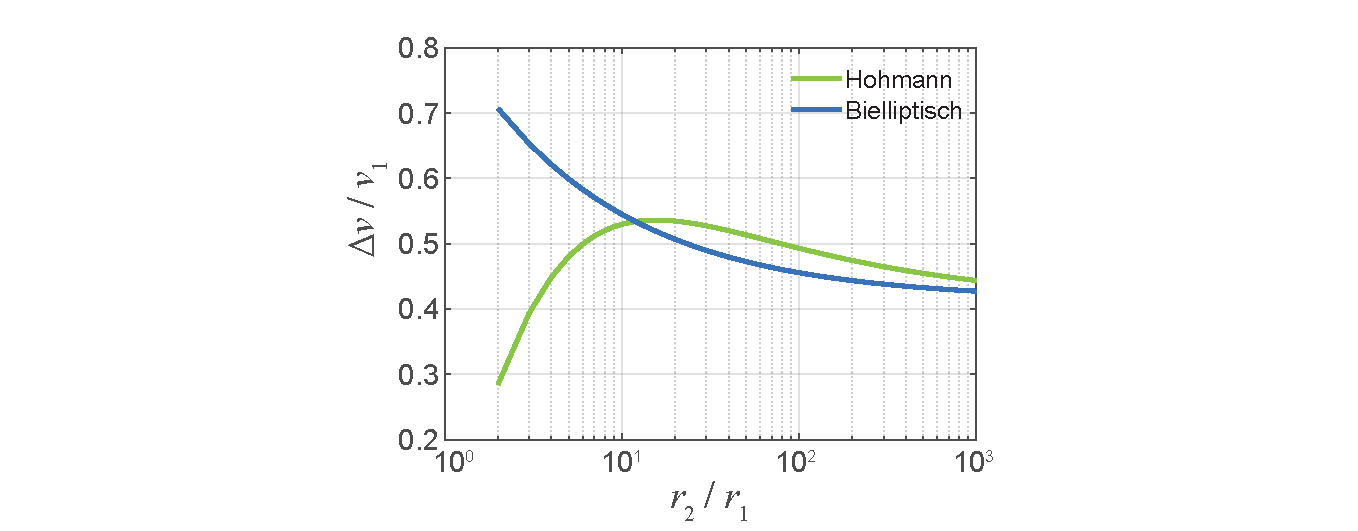
\includegraphics[width=\textwidth]{BiEllptischerTransfer.pdf} 
	\caption[Bielliptischer Transfer.]{Antriebsbedarf beim bielliptischen Transfer im Vergleich zum Hohmann-Transfer.}
	\label{abb:adyn_manoevers2}
\end{figure}

Man erkennt aus \figref{adyn_manoevers2}, dass in der Tat f�r gro�e Radienverh�ltnisse ($\gamma > \SI{11.94}{}$) der bielliptische-Transfer energetisch g�nstiger ist.\\
Allerdings erkauft man sich das durch sehr lange Transferzeiten. Vorteilhaft sind solche bielliptischen �berg�nge aber, wenn man die Inklination und Umlaufrichtung des Orbits �ndern will. Die Rechnungen sind im Detail im \mscr~\mladynref{BiElliptischerTransfer.m} ausgef�hrt.
Die in der Abbildung gezeigten Trajektorien der hyperbolischen Bahnen sind nach \kap{hm_bewegungsgl} gegeben durch:
\begin{align}
	 r = \frac{a\,\lk 1 - e^2 \rk}{1 - e\,\cos\upsilon} ~~~\text{mit}~~~\upsilon < \arccos\frac{1}{e} ~~~\text{und}~~~a = \frac{r_\text{P}}{(1-e)} \,.	\label{eq:adyn_oberth37}
\end{align}
Die geometrischen Parameter $a$ und $e$ der Hyperbel sind durch die physikalischen Parameter $H$ \bzw $v_\infty$ und $r_\text{P}$ definiert (vgl. \kap{hm_bewegungsgl}: $~a < 0,\, e > 1$):
\begin{align}
	 a = -\frac{\mu}{2H_\infty} = -\frac{\mu}{v_\infty{}^2} ~~~\text{und}~~~e = 1 + \frac{r_\text{P}\,v_\infty{}^2}{\mu} \,.	\label{eq:adyn_oberth38}
\end{align}

\end{sol} 
\textcolor{blue} {$\rightarrow$ zur} \probref{adyn_manoevers2}.\\
\noindent\rule[1ex]{\textwidth}{0.5pt}  \newpage  \clearpage

%-----------------------------------------------------------------------------------------------------------

\begin{sol}{prob:adyn_manoevers3}\label{lsg:adyn_manoevers3} %�bung14
\textbf{Hohmann-Oberth-Edelbaum-Transfers aus dem Orbit nach $\infty$}\\

Die Rechnungen sind explizit im \mscr~\mladynref{TransferUnendlich.m} hinterlegt und die Ergebnisse in \figref{adyn_Oberth_transfer2} und \figref{adyn_Oberth_transfer3} gezeigt. 
Man erkennt, dass es f�r gr��ere finale Abst�nde $r_\text{end}$ und bestimmte Verh�ltnisse von $r_{+}/r_1$  ein Minimum der Flugzeit f�r den Edelbaum-Transfer gibt. Er ist in den meisten F�llen der energetisch g�nstigste Transfer. Der Hohmann-Transfer ist f�r gro�e Entfernungen sowohl was die Flugzeit als auch den Antriebsbedarf betrifft der ung�nstigste.\\

\begin{figure}
	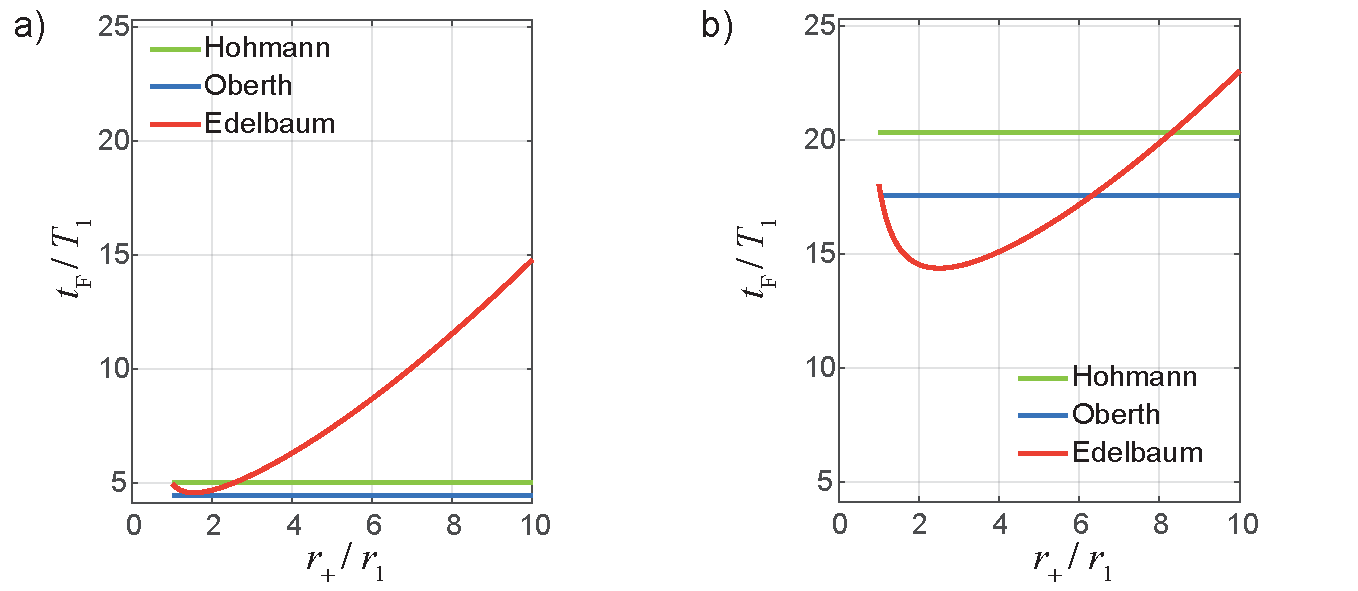
\includegraphics[width=\textwidth]{TransfersInfin03.pdf} 
	\caption[Flugzeiten beim Transfer nach $\infty$.]{Flugzeiten beim Hohmann-, Oberth- \bzw Edelbaum-Transfer. \fa bis zu $r_\text{end}=50\,r_1$ \fb bis zu $r_\text{end}=200\,r_1$.  Als variabler Parameter wurde der �u�ere Radius $r_{+}$ genommen, der innere Radius wurde als fix mit $r_{-}=0.05\,r_1$ gesetzt und der Schubparameter wurde mit $\Delta v/v1 = 1.1$ angenommen. Man erkennt, dass es f�r $r_{+}\approx 2.5\,r_1$ ein absolutes Minimum der Flugzeit f�r den Edelbaum-Transfer gibt. Danach f�hrt die l�ngere Flugzeit auf der Halbellipse von $r_{+}$ nach $r_{-}$ zu insgesamt l�ngeren Flugzeiten.} \label{abb:adyn_Oberth_transfer3}
\end{figure}

\end{sol} 
\textcolor{blue} {$\rightarrow$ zur} \probref{adyn_manoevers3}.\\
\noindent\rule[1ex]{\textwidth}{0.5pt}  \newpage  \clearpage

%-----------------------------------------------------------------------------------------------------------

\begin{sol}{prob:adyn_manoevers4}\label{lsg:adyn_manoevers4} %�bung15
\textbf{Lambert-Problem}\\

Die allgemeine Formulierung des Lambert-Problems lautet wie folgt (\figref{adyn_lambert_lsg02a}):\\
Es seien zwei Punkte $\text{P}_1,\, \text{P}_1$ im Raum durch ihre Vektoren $\vec{r}_1$, $\vec{r}_2$ bekannt, ebenso die Zeit $t_\text{F} = t_2-t_1$, die f�r die Bewegung des K�rpers zwischen $\mathrm{P}_1$ und $\mathrm{P}_2$ ben�tigt wird. Gesucht sind f�r die Kepler-Ellipse die Bahnparameter $a$, $e$, $ \upsilon_0$.\footnote{Wir wollen hier nur Ellipsenbahnen betrachten. Man kann das Problem auch f�r Hyperbelbahnen formulieren und l�sen, siehe \ua \cite{Izzo2015, Walter2018}. Im wesentlichen werden dabei die Winkelfunktionen durch die Hyperbelfunktionen ersetzt.}\\

\begin{figure}[H]
	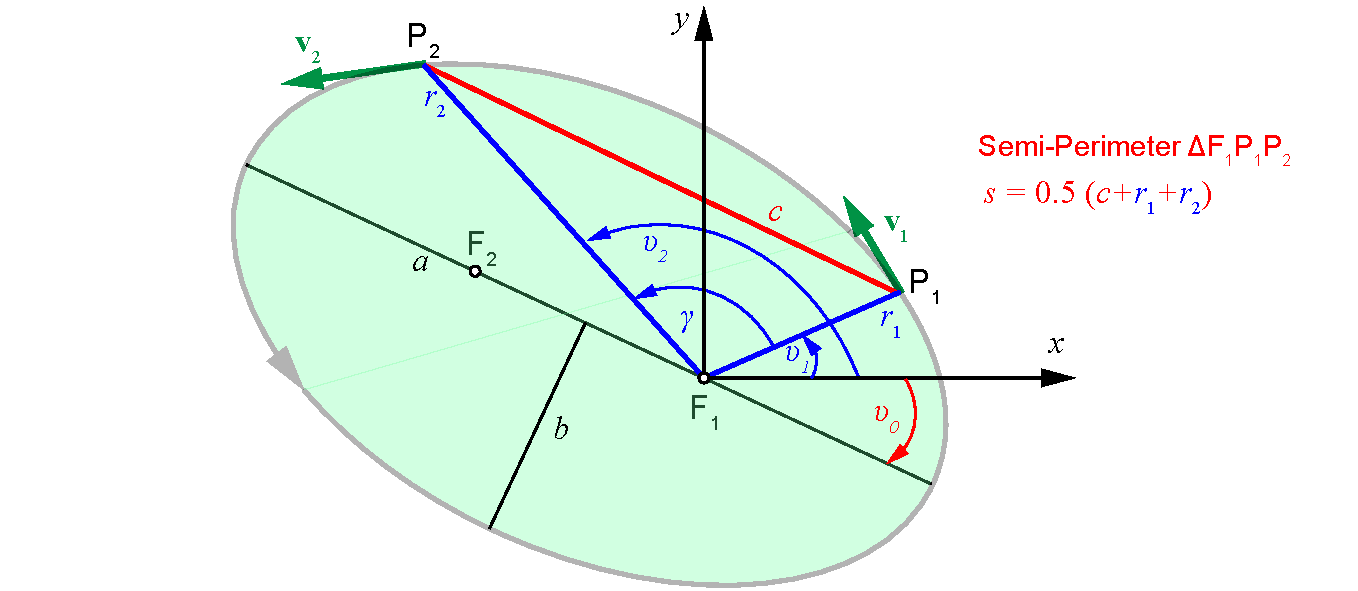
\includegraphics[width=\textwidth]{LambertProblem02Geometrie.pdf} 
	\caption[Geometrie des Lambert-Problems.]{Geometrie des Lambert-Problems. Parameter siehe Text.}
	\label{abb:adyn_lambert_lsg02a}
\end{figure}

Zun�chst schreiben wir die Kepler-Gleichung f�r die beiden Zeitpunkte auf ($\mu$ ist hierin der Gravitationsparameter des Zentralk�rpers, in dessen Schwerefeld die Bewegung stattfindet.) und subtrahieren die beiden Gleichungen voneinander. Wir erhalten:
\begin{align}
\sqrt{\frac{\mu}{a^3}}\,\lk t_2-t_1\rk &= \sqrt{\frac{\mu}{a^3}}\,t_\text{F} = E\lk t_2\rk - E\lk t_1\rk -e\,\lek \sin E\lk t_2\rk -\sin E\lk t_1\rk\rek \nonumber \\
\rightarrow ~~~~ \sqrt{\frac{\mu}{a^3}} \,t_\text{F} &= E_2-E_1 -e\,\lk \sin E_2 -\sin E_1\rk \label{eq:adyn_lsglambert01}\,.
\end{align}
Durch die Randwerte ist ja ein Brennpunkt der Ellipse, n�mlich $\mathrm{F}_1$ bekannt. Man sucht nun den Brennpunkt $\mathrm{F}_2$ (oft auch versteckter Fokus genannt), mit dem dann die Ellipse eindeutig definiert ist und zugleich die Bedingung erf�llt ist, dass f�r das Durchlaufen von $\mathrm{P}_1$ nach $\mathrm{P}_2$ die Zeit $t_\text{F}$, im Englischen auch \gls{ToF} (ToF), ben�tigt wird. 

\begin{figure}[H]
	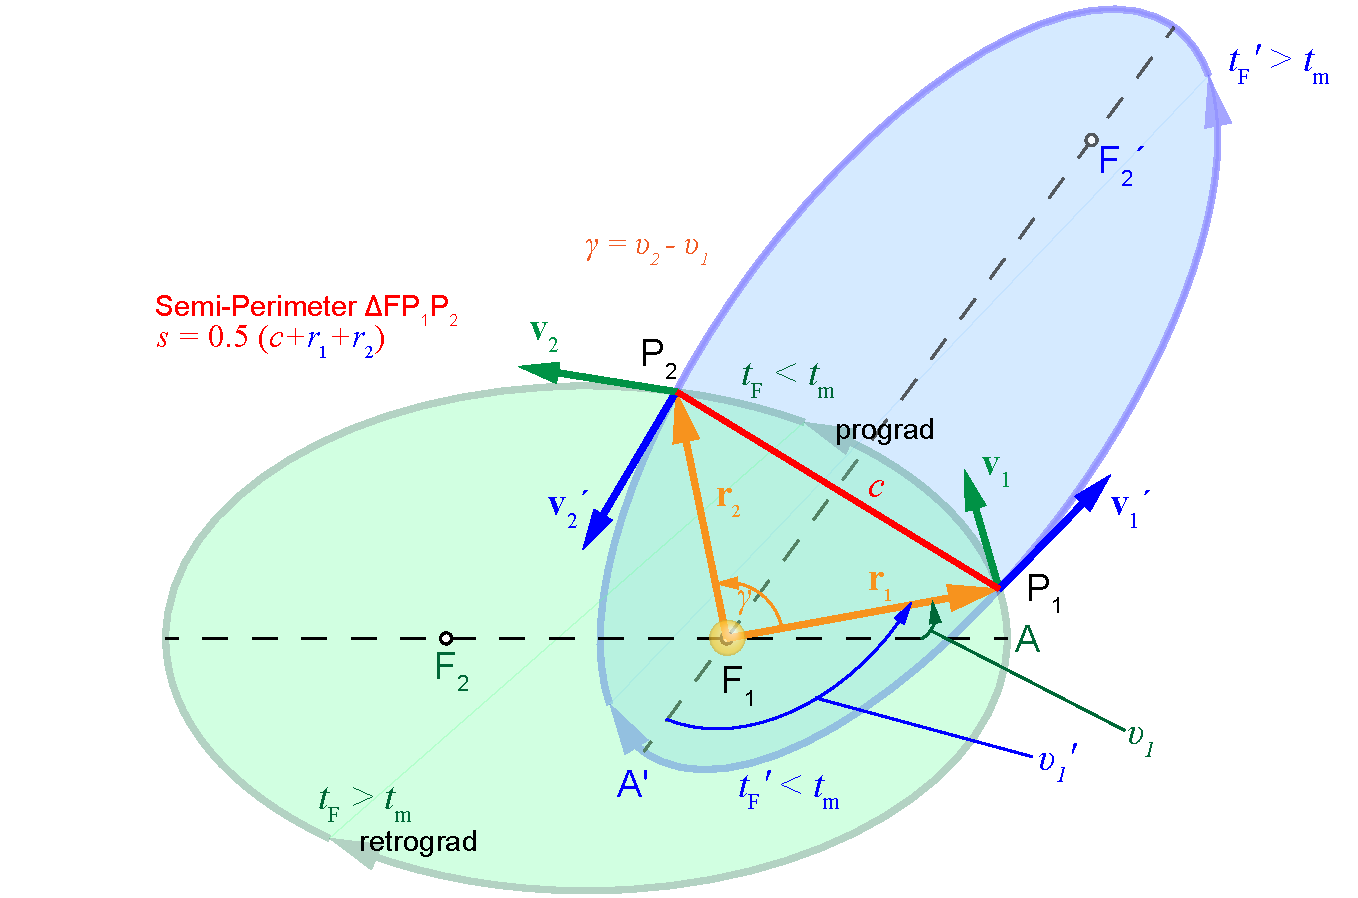
\includegraphics[width=\textwidth]{LambertProblem02Allgemein.pdf} 
	\caption[Geometrie des Lambert-Problems.]{Geometrie des Lambert-Problems. Die beiden Ellipsen (gr�n und blau schattiert) stellen jeweils eine L�sung des Lambert-Problems f�r unterschiedliche Flugzeiten und Flugrichtungen dar. Die Flugrichtung wird als prograd bezeichnet, wenn diese entgegen des Uhrzeigersinns von $\mathrm{P}_1$ nach $\mathrm{P}_2$ erfolgt, die entgegengesetzte Flugrichtung wird retrograd genannt. Die Vektoren $\vec{r}_1$, $\vec{r}_2$ definieren die Ellipsen, sie k�nnen als Positionsvektoren aber auch zu unterschiedlichen Umlaufbahnen geh�ren, \zb $\vec{r}_1$ kann ein Vektor von der Sonne zur Erde sein, $\vec{r}_2$ eine entsprechender Vektor zum Mars. Weitere Parameter siehe Text.}
	\label{abb:adyn_lambert_lsg02}
\end{figure}
Wir k�nnen uns nun leicht �berlegen, dass es f�r die gesuchte Bahn zwei Ellipsen als denkbare L�sungen gibt und zwar mit den beiden "`versteckten"' Fokuspunkten $\mathrm{F}_2$ und $\mathrm{F}_2{}'$ (\figref{adyn_lambert_lsg02})\footnote{Man kann sich die zwei L�sungen anschaulich-geometrisch deutlich machen, in dem man sich die Konstruktionsvorschrift einer Ellipse in Erinnerung ruft. Nach dieser ist an jedem Punkt einer Ellipse die Summe des Abstandes zu den beiden Fokuspunkten konstant und gleich $2a$. Die Konstruktion erfolgt, in dem man einen Kreis um $\mathrm{P}_1$ mit dem Radius $2a-r_1$ schl�gt und einen um $\mathrm{P}_2$ mit $2a-r_2$. Es ergeben sich zwei Schnittpunkte, dies sind die Brennpunkte $\mathrm{F}_2$ \bzw $\mathrm{F}_2{}'$.}.\\
Mit den Beziehung \eqref{eq:hm_r_param_ellipse} und \eqref{eq:hm_bahnglg} aus dem \kap{hm_abl_kepler} k�nnen wir schreiben: 
\begin{subequations}
\begin{align}
    r_{1,2} &= a\,\lk 1-e\,\cos E_{1,2}\rk  \label{eq:adyn_lsglambert02a} \,,\\
    \cos\lk \upsilon_{1,2}-\upsilon_0\rk &= \frac{a}{r_{1,2}}\,\lk\cos E_{1,2}-e\rk \,. \label{eq:adyn_lsglambert02b}
    %r_{1,2}\cos{\upsilon_{1,2}} &= a\,\lk \cos E_{1,2} - e \rk \,, \label{eq:adyn_lsglambert02b} \\
    %r_{1,2}\sin{\upsilon_{1,2}} &= a\,\sqrt{\lk 1-e^2 \rk}\, \sin E_{1,2} \,, \label{eq:adyn_lsglambert02c} \\
\end{align} %\label{eq:adyn_lsglambert02} 
\end{subequations}
Wir betrachten eine der beiden Ellipsen aus \figref{adyn_lambert_lsg02} genauer und verwenden die Darstellung in \figref{adyn_lambert_lsg02a}. Unser Ziel ist es ja, die Trajektorie $r(\upsilon)$ zu finden:
\begin{align}
    r (\upsilon) &= \frac{a\,\lk 1 - e^2 \rk}{1+e\,\cos\lk\upsilon - \upsilon_0 \rk}\,. \label{eq:adyn_lsglambert_traj} 
\end{align} 
In einer Ebene ist eine Trajektorie (Bahn) durch 3 Parameter eindeutig bestimmt. Das Lambert-Problem ist ein planares Problem und wir
haben mit dem Gleichungssystem \eqref{eq:adyn_lsglambert01}, \eqref{eq:adyn_lsglambert02a} und \eqref{eq:adyn_lsglambert02b} ein System f�r 5 Unbekannte $E_1$, $E_2$, $a$, $e$, $\upsilon_0$ mit den bekannten Gr��en $r_1$, $r_2$, $\upsilon_1$, $\upsilon_2$, $t_\text{F}$ und $\mu$.\footnote{Eigentlich sind $\upsilon_1$, $\upsilon_2$ ja nicht bekannt, sondern nur deren Differenz. Durch freie Festlegung eines \KOS wie in \figref{adyn_lambert_lsg02a} gezeigt kann man sich aber $\upsilon_1$ und $\upsilon_2$ berechnen. Man beachte, dass dieses \KOS mit den $x-y$- Achsen in der Ellipsenebene liegt und gegebenenfalls durch Drehung in ein anderes (\zb heliozentrisches) \KOS transformiert werden muss, wenn man die koordinaten der Trajektorie in diesem haben  m�chte.} Dieses System wollen wir jetzt l�sen:
\begin{enumerate}
    \item [1.] Mit der Nebenrechnung (\cite{Gradshteyn1980})
		\begin{align*}
		\sin x - \sin y =&  \sin{\lk \frac{x-y}{2} +  \frac{x+y}{2}\rk} - \sin{\lk \frac{x+y}{2} +  \frac{-x+y}{2}\rk} \\
		=& \sin{\lk \frac{x-y}{2} +  \frac{x+y}{2}\rk} + \sin{\lk \frac{x-y}{2} + \frac{-x-y}{2} \rk} \\
		=& \sin\lk \frac{x-y}{2}\rk\,\cos\lk\frac{x+y}{2}\rk + \sin\lk \frac{x+y}{2}\rk\,\cos\lk\frac{x-y}{2}\rk\\
		&+ \sin\lk \frac{x-y}{2}\rk\,\cos\lk\frac{x+y}{2}\rk - \sin\lk \frac{x+y}{2}\rk\,\cos\lk\frac{x-y}{2}\rk \\
		=& 2\,\sin{\frac{x-y}{2}}\,\cos{\frac{x+y}{2}}
		\end{align*}
    f�hren wir $\psi$ und $\varphi$ als neue Variable ein:
    \begin{align}
        \psi = \frac{E_2-E_1}{2}~~~~ \text{und} ~~~~ \cos \varphi = e\,\cos\lk \frac{E_2 +E_1}{2} \rk \,, \label{eq:adyn_lsglambert06}
    \end{align}
		wobei $\psi \in [0, \pi]$ und $\varphi \in [0, \pi]$ gilt. Wir erhalten dann die Kepler-Gleichung \eqref{eq:adyn_lsglambert01} in folgender vereinfachter Form:
\begin{align}
			\sqrt{\frac{\mu}{a^3}} \,t_\text{F} &= \psi - \cos\varphi\, \sin\psi \label{eq:adyn_lsglambert01a}\,.
\end{align}
Die beiden Gr��en $\psi$ und $\varphi$ h�ngen nur von der vorgegebenen Geometrie des Problems ab, wie man leicht nachrechnen kann, in dem man 
den Abstand von $\mathrm{P}_1$ und $\mathrm{P}_2$ unter Verwendung von \eqref{eq:adyn_lsglambert02b} �ber 
    \begin{align}
        c^2 &= \lk r_2\,\cos\upsilon_2 - r_1\,\cos\upsilon_1 \rk^2 + \lk r_2\,\sin\upsilon_2 - r_1\,\sin\upsilon_1 \rk^2 ~\nonumber \\
				&= r_1{}^2+r_2{}^2 - 2\,r_1\,r_2\,\cos\lk \upsilon_2-\upsilon_1\rk = r_1{}^2+r_2{}^2 - 2\,r_1\,r_2\,\cos\lk \gamma \rk~\nonumber \\
				\rightarrow~~c &= 2 a\,\sin\psi\,\sin\varphi\, \label{eq:adyn_lsglambert03a}
    \end{align}
berechnet. 
Ebenso erh�lt man die Summe der Abst�nde $r_1+r_2$ von den Punkten $\mathrm{P}_1$ und $\mathrm{P}_2$ zum Brennpunkt $\mathrm{F}_1$ wiederum unter Verwendung von \eqref{eq:adyn_lsglambert02b} zu
		\begin{align}
		r_1 + r_2  &= 2a\lk 1- \cos\psi\, \cos\varphi \rk\,. \label{eq:adyn_lsglambert03b}
    \end{align} 
Die Gleichungen \eqref{eq:adyn_lsglambert03a} und \eqref{eq:adyn_lsglambert03b} bestimmen die Gr��en $\psi$ und $\varphi$ eindeutig. Man kann also schlussfolgern, dass die Zeit $t_\text{F}$ nach \eqref{eq:adyn_lsglambert01a} nur eine Funktion von $a$ und den bekannten geometrischen Gr��en $c$ und $r_1 + r_2$  ist.\footnote{Der Beweis daf�r wurde von Lagrange erbracht, der zeigte, dass die ToF $t_\text{F}$ nur von der Energie der Bahn und damit nur von $a$ abh�ngt.}\\   

\item [2.] Um uns die Rechnungen zu erleichtern, f�hren wir zwei weitere Gr��en ein, die wir aus $\varphi$ und $\psi$ wie folgt bilden:
				\begin{align}
						\alpha= \varphi +\psi ~~~~ \text{und} ~~~~ \beta= \varphi-\psi \,. \label{eq:adyn_lsglambert05}
				\end{align}
		Offensichtlich gilt: $\alpha \in [0,\, 2\pi]$ und $\beta \in [-\pi,\, \pi]$. \\
		
\item [3.] Wir bezeichnen den halben Umfang (Semi-Perimeter) des Dreiecks $\Delta \,\mathrm{F}_1\mathrm{P}_1\mathrm{P}_2$ mit 
    \begin{align}
        s= \frac{r_1+r_2+c}{2}\,. \label{eq:adyn_lsglambert04}
    \end{align}
		Damit und mit \eqref{eq:adyn_lsglambert03a} und \eqref{eq:adyn_lsglambert03b} findet man  f�r $\alpha$ die Beziehung: 
    \begin{subequations}
    \begin{align}
        \frac{s}{2a} &= \frac{1}{2} \lek 1 - \cos\psi\cos\varphi + \sin\psi\sin\varphi \rek = \frac{1}{2} \lek 1 - \cos \lk \psi+\varphi \rk \rek \nonumber \\
				&= \frac{1}{2} \lek 1 - \cos\alpha \rek = \frac{1}{2} \lek 1 - \cos\lk \frac{\alpha}{2} + \frac{\alpha}{2} \rk \rek \nonumber \\
				&= \frac{1}{2} \lek 1 - \cos^2\frac{\alpha}{2} + \sin^2\frac{\alpha}{2} \rek = \frac{1}{2} \lek 2\sin^2\frac{\alpha}{2} \rek \nonumber \\
        &\rightarrow~~ \sin^2\lk \frac{\alpha}{2}\rk = \frac{s}{2a}\, \label{eq:adyn_lsglambert06a} \\
				&\text{und entsprechend f�r}~~ \beta \nonumber \\
        &\rightarrow~~ \sin^2\lk\frac{\beta}{2}\rk = \frac{s-c}{2a}\,\label{eq:adyn_lsglambert06b}
    \end{align}
    \end{subequations}
    Sowohl $\alpha$ als auch $\beta$ sind somit Gr��en, die nur von der Geometrie der Aufgabenstellung und dem Bahnparameter $a$ abh�ngen.\\
		
\item [4.] Wir setzen nun \eqref{eq:adyn_lsglambert06a} und \eqref{eq:adyn_lsglambert06b} in \eqref{eq:adyn_lsglambert01} ein und erhalten die elegante Formulierung des Lambert-Problems 
\begin{align}
    t_\text{F} &= \sqrt{\frac{a^3}{\mu}}\,\lk \alpha-\beta-\lek\sin\alpha -\sin\beta\rek\rk\,,\label{eq:adyn_lsglambert07}
\end{align}   
Damit haben wir $E_2$, $E_1$ aus der Kepler-Gleichung eliminiert und das Lambert-Problem auf ein System von 3 Unbekannten ($a$, $\alpha$, $\beta$) zur�ck gef�hrt, von den $\alpha$ und $\beta$ neben den bekannten Gr��en $s$, $c$ nur noch von $a$ abh�ngen. Der Winkel $\alpha$ ist dabei wegen des Quadrats in \eqref{eq:adyn_lsglambert06a} nicht eindeutig bestimmt, es gibt zwei L�sungen
\begin{align}
	\alpha ~~~\text{und}~~~ \alpha'=2\pi-\alpha\,, \label{eq:adyn_lsglambert08}
\end{align}
die den beiden Ellipsenl�sungen und damit auch den beiden Zeit $t_\text{F}$ \bzw $t_\text{F}'$ in \figref{adyn_lambert_lsg02} entsprechen. Der Wert f�r $\beta$ ist hingegen f�r ein aus \eqref{eq:adyn_lsglambert08} folgendes  $a$ \bzw $a'$ eindeutig bestimmt. Man muss aber folgende Fallunterscheidung machen: 
\begin{align}
    \beta = \left\{
\begin{array}{ll}
+2\arcsin\sqrt{(s-c)/a} ~~ & \text{f�r} ~~~~ \gamma = \upsilon_2-\upsilon_1 <\pi \\
-2\arcsin\sqrt{(s-c)/a} ~~ & \text{f�r} ~~~~ \gamma = \upsilon_2-\upsilon_1 >\pi \\
\end{array}
\right.\,.\label{eq:adyn_lsglambert09}
\end{align}

\item [5.] Setzen wir $\alpha\lk a,a' \rk$ und $\beta\lk a,a' \rk$ in \eqref{eq:adyn_lsglambert07} ein, erhalten wir demzufolge zwei Kurven $t_\text{F}\lk a\rk$, die vom Punkt $\lek a_\text{min},\, t_\text{m} \rek$ ausgehen (siehe \figref{adyn_lambert_lsg03}). Hierbei ist $a_\text{min} = s/2$, wie man leicht nachpr�fen kann. Die Ellipse, die durch $a_\text{min}$ definiert wird auch Minimal-Energie-Bahn genannt, wegen $E_\text{min}= -\mu/(2a_\text{min})$. Das ist aber nicht zu verwechseln mit dem minimalen Antriebsbedarf $\Delta v_\text{min}$. Ebenso ist $t_\text{m}$ nicht die minimale Flugzeit, sondern die Flugzeit f�r die Bahn mit der kleinsten Bahnenergie. Wie bereits erw�hnt und aus \figref{adyn_lambert_lsg02} zu erkennen, gibt es zu einem bestimmten Wert von $a$ zwei ToF, die dem kurzen ($t_\text{F} < t_\text{m}$) \bzw  der dem langen Transfer ($t_\text{F} > t_\text{m}$) von $\mathrm{P}_1$ nach $\mathrm{P}_2$ entsprechen.\end{enumerate}

Wir wollen nun Gleichung \eqref{eq:adyn_lsglambert07} l�sen. Das ist analytisch nicht m�glich. Da sie aber eine gewisse �hnlichkeit mit der Kepler-Gleichung hat, k�nnen wir �hnliche Iterationsmethoden wie in \kap{iteration_kepler} benutzen. Wir wollen hier das sogenannte Bisektionsverfahren \cite{Arens2008} verwenden. Man geht folgenderma�en vor:
\begin{enumerate}
    %1.
    \item [1.] Wir bestimmenen die Flugzeit f�r eine Parabell�sung von $\text{P}_1$ nach $\text{P}_2$. Diese l�sst sich aus der Barker-Gleichung\index{Barker-Gleichung} \eqref{eq:hm_Barker_glg} bestimmen:\footnote{F�r die interessierten Leser empfehlen wir die Herleitung von \eqref{eq:adyn_lsglambert11} aus der Barker-Gleichung\index{Barker-Gleichung} \eqref{eq:hm_Barker_glg} (siehe  \kap{kometen}) nachzuvollziehen.} % und verweisen auf die Referenzen \cite{Izzo2015}, \cite{Sangra2021}
			\begin{align}
								t_\text{Par} &= \frac{\sqrt{2}}{3}\,\sqrt{\frac{s^3}{\mu}}\,\lk 1-\sqrt{\lk\frac{s-c}{s}\rk^3}\rk\,.\label{eq:adyn_lsglambert11}
			\end{align}
    %2.
    \item [2.] Wir definieren mit \eqref{eq:adyn_lsglambert07} die Funktion\\
			\begin{align}
						\tau\lk a\rk &= \sqrt{\frac{a^3}{\mu}}\,\lek \alpha\lk a\rk -\beta\lk a \rk - \lk \sin\alpha\lk a\rk-\sin\beta\lk a\rk \rk\rek\,.\label{eq:adyn_lsglambert11a}
			\end{align}
    Gesucht ist das $a$, welches $\tau\lk a\rk = t_\text{F}$ erf�llt.
    %3.
    \item [3.] Wir setzen nun $a_\text{min} = s/2$ und bestimmen damit $t_\text{m} = \tau\lk a_\text{min} \rk$. Ist $t_\text{m} > t_\text{F} > t_\text{Par}$,
		so muss eine (elliptische) L�sung existieren.\footnote{F�r $t_\text{F} < t_\text{Par}$ kann man einen hyperbolischen Transfer von $\mathrm{P}_1$ nach $\mathrm{P}_2$ finden, der noch schneller als der parabolische ist. Wir verweisen auf \cite{Izzo2015, Walter2018}.} Ist $t_\text{Par} < t_\text{F} < t_\text{m}$, dann gibt es eine L�sung auf dem unteren Ast in \figref{adyn_lambert_lsg03}, f�r $t_\text{F} > t_\text{m}$ kann es eine L�sung auf dem oberen Ast geben. Man muss das Bisektionsverfahren entsprechend anpassen, siehe dazu auch \mscr~\mladynref{LambertProblem02.m}. 
    %4.
    \item [4.] Wir suchen nun ein $a_\text{max} \gg a_\text{min}$ und setzen $a_1 = (a_\text{min} + a_\text{max})/2$.
    %5.
    \item [5.] Wir bestimmen $\tau\lk a_1\rk$.
    %6.
    \item [6.] Falls $\tau\lk a_1\rk> t_\text{F}$, dann setzen wir $a_2= (a_1+a_\text{max})/2$, falls $\tau\lk a_1\rk <t_\text{F}$, dann setzen wir $a_2 = (a_\text{min}+a_1)/2$.
    %7.
    \item [7.] Wir wiederholen die Schritte bis zur gew�nschten Genauigkeit von $\tau\lk a_n\rk \approx t_\text{F}$. 
\end{enumerate}
Dieses Verfahren konvergiert, falls �berhaupt eine L�sung existiert: deshalb muss man im Schritt 1 �berpr�fen, ob f�r die gegebenen Werte $r_1$, $r_2$, $\gamma$ und $t_\text{F}$ �berhaupt eine elliptische L�sung existiert. 

\begin{figure}[H]
	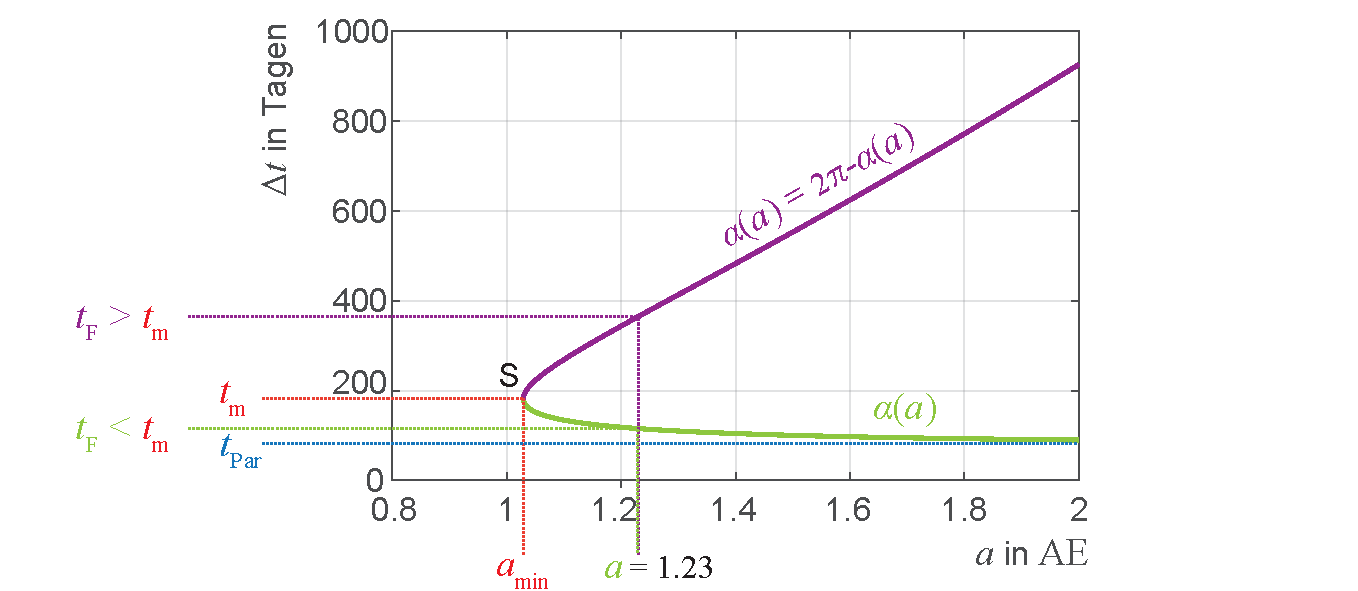
\includegraphics[width=\textwidth]{LambertProblem02Zeiten.pdf} 
	\caption[L�sung des Lambert-Problems.]{L�sung des Lambert-Problems f�r folgende Parameter: $r_1 = \SI{1.0}{AE},\, r_2 = \SI{1.525}{AE},\, \gamma = 75\degree$, und einer ToF von $t_\text{F} = 115 \mathrm{d}$ \bzw $t_\text{F} = 365 \mathrm{d}.$ Siehe \mscr~\mladynref{LambertProblem02.m}.}
	\label{abb:adyn_lambert_lsg03}
\end{figure}
Wir brauchen jetzt noch, nachdem wir $a$ bestimmt haben, die Bahnparameter $e$ und $\upsilon_0$. Aus \eqref{eq:adyn_lsglambert02a} finden wir 
\begin{align}
    E_1 = \arccos \lk \frac{a-r_1}{a\,e} \rk  \label{eq:adyn_lsglambert13}
\end{align}
und aus \eqref{eq:adyn_lsglambert02b} auch $\upsilon_0$
\begin{align}
    \upsilon_0 = \upsilon_1 - 2\,\arctan\lk \sqrt{\frac{1+e}{1-e}}\,\tan\frac{E_1}{2}\rk\,.  \label{eq:adyn_lsglambert14}
\end{align}
Setzen wir das gefundene $a$ in die Gleichungen f�r $\alpha$ und $\beta$ ein und diese wiederum in die f�r $\varphi$ und $\psi$ finden wir mit \eqref{eq:adyn_lsglambert02b} f�r die Exzentrizit�t
\begin{align}
    e = \sqrt{\frac{\lk r_2-r_1\rk^2}{\lk2a\,\sin\psi\rk^2}+\cos^2\varphi}\,.  \label{eq:adyn_lsglambert15}
\end{align}

Hat man mittels Bisektionsverfahren entweder $p$  (mit \mscr~\mladynref{LambertProblem01.m}) oder $a$  (mit \mscr~\mladynref{LambertProblem02.m}) bestimmt, kann man �ber folgende  Beziehung die Geschwindigkeiten an den Punkten $\mathrm{P}_1$ nach $\mathrm{P}_2$ auf der Trajektorie bestimmen (\cite{Walter2018, Battin1999}:
\begin{align}
\begin{split}
    \vec{v}_\text{tr, 1} &= \sqrt{\frac{\mu\,p}{r_1\,r_2\,\sin\gamma}}\,\lek \lk \vec{r}_2 - \vec{r}_1 \rk  + \frac{r_2}{p}\,\lk 1- \cos\gamma \rk\,\vec{r}_1 \rek \\
    \vec{v}_\text{tr, 2} &= \sqrt{\frac{\mu\,p}{r_1\,r_2\,\sin\gamma}}\,\lek \lk \vec{r}_2 - \vec{r}_1 \rk  + \frac{r_1}{p}\,\lk 1- \cos\gamma \rk\,\vec{r}_2 \rek \,.
\end{split}  \label{eq:adyn_lambert16}
\end{align}
Die Richtung der Periapsis (Perihel, Perig�um \usw) und damit der Wert f�r $\upsilon_0$ kann dann �ber den Laplace-Vektor\index{Laplace-Vektor} $\vec{e}$ und \eqref{eq:hm_laplace_int} aus \kap{hm_abl_kepler} wie folgt bestimmt werden:
\begin{align}
    \vec{e} &= \lk \frac{1}{r_1} - \frac{1}{a} \rk \, \vec{r}_1  - \frac{1}{\mu} \, \lk \vec{r}_1 \cdot \vec{v}_\text{tr, 1} \rk \, \vec{v}_\text{tr, 1} \,. 
		\label{eq:adyn_lambert17}
\end{align}

Wir haben das Bisektionsverfahren zur L�sung des Lambert-Problems exemplarisch f�r zwei verschiedene F�lle im \mscr~\mladynref{LambertProblem01.m} \bzw \mscr~\mladynref{LambertProblem02.m} hinterlegt. Fall 1 ist der Transfer einer Raumsonde von der ISS aus $h \approx \SI{422}{\km}$ in die Stratosph�re ($h \approx \SI{22}{\km}$) innerhalb von 50 min und Fall 2 ein Raumflug von der Erde zum Mars f�r eine Flugdauer von 115 Tagen. \figref{adyn_lambert_lsg04} und Tabelle \ref{tab:adyn_bisection} zeigen den Verlauf der Iteration f�r den Fall 2.\\

Im \mscr~\mladynref{LambertProblem03.m} haben wir die Rechnungen mit einer modernen, stabileren numerischen Routine zur L�sung des Lambert-Problems (\cite{Mahooti2015}) wiederholt. Die Routine basiert auf den Ans�tzen, die in \cite{Battin1999, Izzo2015, Walter2018} ausf�hrlich beschrieben sind. Sie beinhaltet auch hyperbolische L�sungen. Die �bereinstimmung mit dem Bisektionsverfahren f�r die angegebenen Beispiele ist sehr gut.

\begin{figure}[H]
	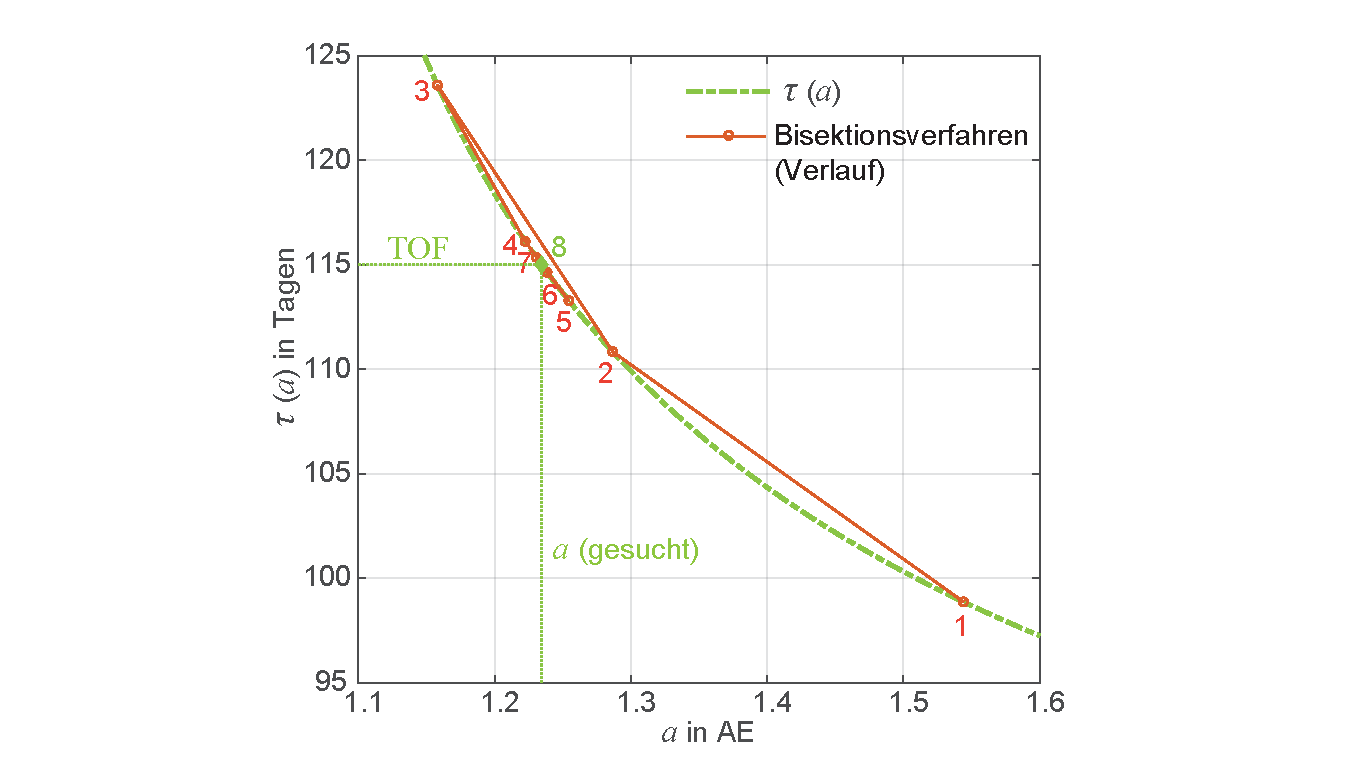
\includegraphics[width=\textwidth]{BisektionLambert.pdf} 
	\caption[Bisektionsverfahren zur L�sung des Lambert-Problems.]{Bisektionsverfahren zur L�sung des Lambert-Problems f�r folgende Parameter: $r_1 = \SI{1.000}{AE},\, r_2 = \SI{1.525}{AE},\, \gamma = 75\degree$, und einer ToF von $t_\text{F} = 115\,\mathrm{d}$. Siehe \mscr~\mladynref{LambertProblem02.m}.}
	\label{abb:adyn_lambert_lsg04}
\end{figure}

\begin{table}[ht]
\begin{center}
\begin{tabular}{L{1cm}R{1.5cm}R{1.5cm}R{1.5cm}R{2cm}R{2cm}R{1.5cm}}
    \hline
    \rule{0pt}{3pt}&&&&&& \\
      $n$ & $a_n$ & $\alpha_n$ & $\beta_n$ & $\tau(\alpha_n)$ & $\tau(\alpha_n) - \mathrm{ToF} $ & $e_n$\\
    %\rule{0pt}{3pt}&&&&&& \\
       & $\SI{}{AE}$ &&& Tage & Tage & \\
    \rule{0pt}{3pt}&&&&&& \\
    \hline
    \rule{0pt}{3pt}&&&&&& \\
 \rule{0pt}{3pt} 1    &   1.544     &   1.911    &   0.798     &   98.87      &   -16.132      &   0.387 \\
 \rule{0pt}{3pt} 2    &   1.287     &   2.214    &   0.879     &  110.83      &    -4.166      &   0.330 \\
 \rule{0pt}{3pt} 3    &   1.158     &   2.462    &   0.931     &  123.60      &     8.596      &   0.350 \\
 \rule{0pt}{3pt} 4    &   1.222     &   2.324    &   0.904     &  116.12      &     1.120      &   0.332 \\
 \rule{0pt}{3pt} 5    &   1.255     &   2.267    &   0.891     &  113.28      &    -1.723      &   0.330 \\
 \rule{0pt}{3pt} 6    &   1.238     &   2.295    &   0.898     &  114.64      &    -0.358      &   0.331 \\
 \rule{0pt}{3pt} 7    &   1.230     &   2.309    &   0.901     &  115.37      &     0.366      &   0.331 \\
 \rule{0pt}{3pt} 8    &   1.234     &   2.302    &   0.899     &  115.00      &     0.000      &   0.331 \\
    \rule{0pt}{3pt}&&&&&& \\
    \hline
\end{tabular}    
\end{center}
\caption{Bisektionsverfahren zur L�sung des Lambert-Problems. Parameter siehe Text \bzw \figref{adyn_lambert_lsg04}.}
 %f�r folgende Parameter: $r_1 = \SI{1.0}{AE},\, r_2 = \SI{1.525}{AE},\, \gamma = 75\degree$, und einer ToF von $t_\text{F} = 115 \mathrm{d}$ \bzw $t_\text{F} = 365 \mathrm{d}.$ Siehe \mscr\mladynref{LambertProblem02.m}.}
\label{tab:adyn_bisection}
\end{table}


\end{sol} 

\textcolor{blue} {$\rightarrow$ zur} \probref{adyn_manoevers4}.\\
\noindent\rule[1ex]{\textwidth}{0.5pt}  \newpage  \clearpage

%-----------------------------------------------------------------------------------------------------------

\begin{sol}{prob:adyn_manoevers5}\label{lsg:adyn_manoevers5} %�bung16
\textbf{Venus- und Mars-Fl�ge}\\

Wir bestimmen als erstes die Flugzeit f�r eine Parabell�sung von der Erdbahn (Punkt $\text{P}_1$) zur Marsbahn (Punkt $\text{P}_2$). Diese l�sst sich aus der Barker-Gleichung\index{Barker-Gleichung} \eqref{eq:hm_Barker_glg} bestimmen (siehe L�sung zu \probref{adyn_manoevers4} und\cite{Izzo2015}, \cite{sangra2021}):
			\begin{align}
								t_\text{Par} &= \frac{\sqrt{2}}{3}\,\sqrt{\frac{s^3}{\mu}}\,\lk 1-\sqrt{\lk\frac{s-c}{s}\rk^3}\rk\,.\label{eq:adyn_lsglambert21}
			\end{align}
Wir verweisen auf das \mscr~\mladynref{FlugVenusParabelbahn.m}, in welchem die Parabel-Flugbahn einer Raumsonde zur Venus
zu verschiedenen Startzeiten auf Basis der der L�sung des Lambert-Problems numerisch berechnet wird. Vorgegeben ist das Startdatum, gesucht ist das Ankunftsdatum mit dem
schnellsten Transfer unab�ngig vom notwendigen Antriebsbedarf.

\begin{figure}[H]
	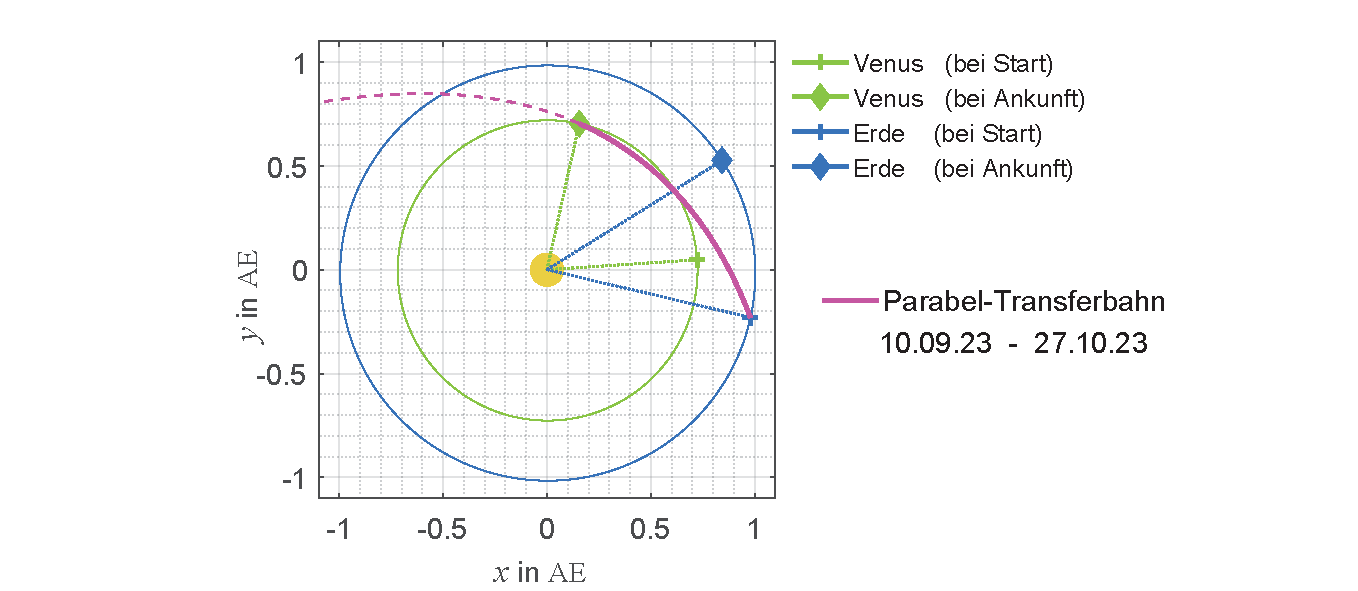
\includegraphics[width=\textwidth]{ParabelTransferVenus.pdf} 
	\caption[Parabel-L�sung des Lambert-Problems.]{Parabel-L�sung des Lambert-Problems f�r einen Flug zur Venus. Siehe \mscr~\mladynref{FlugVenusParabelbahn.m}.}
	\label{abb:adyn_lambert_lsg05}
\end{figure}

F�r die Berechnung der Transferbahn (elliptisch) von der Erde zur Venus oder zum Mars bei vorgegebener ToF benutzen wir die \mscr~\mladynref{LambertProblem03.m} \bzw \mladynref{LambertMarsVenus.m}, in welchen �ber die Routine \mladyniref{LambertSolver3.m}. die Parameter des interplanetaren Raumflugs zum Mars bzw. zur Venus �ber die L�sung des Lambert-Problems berechnet werden. Vorgegeben sind dabei die Positionsvektoren 1 und 2, sowie die Abflug und Ankunftszeit. Die Abflugs-Ankunfs-Positionen m�ssen vorher berechnet werden (z.B. �ber \mscr~\mladynref{FlugzeitenMarsVenus.m} oder �ber Programme aus dem Kapitel Himmelsmechanik, wie \mscr~\mlhmref{PlanetenbahnenKepler.m} und \mlhmref{PlanetenPositionen.m}. \\

\begin{figure}[H]
	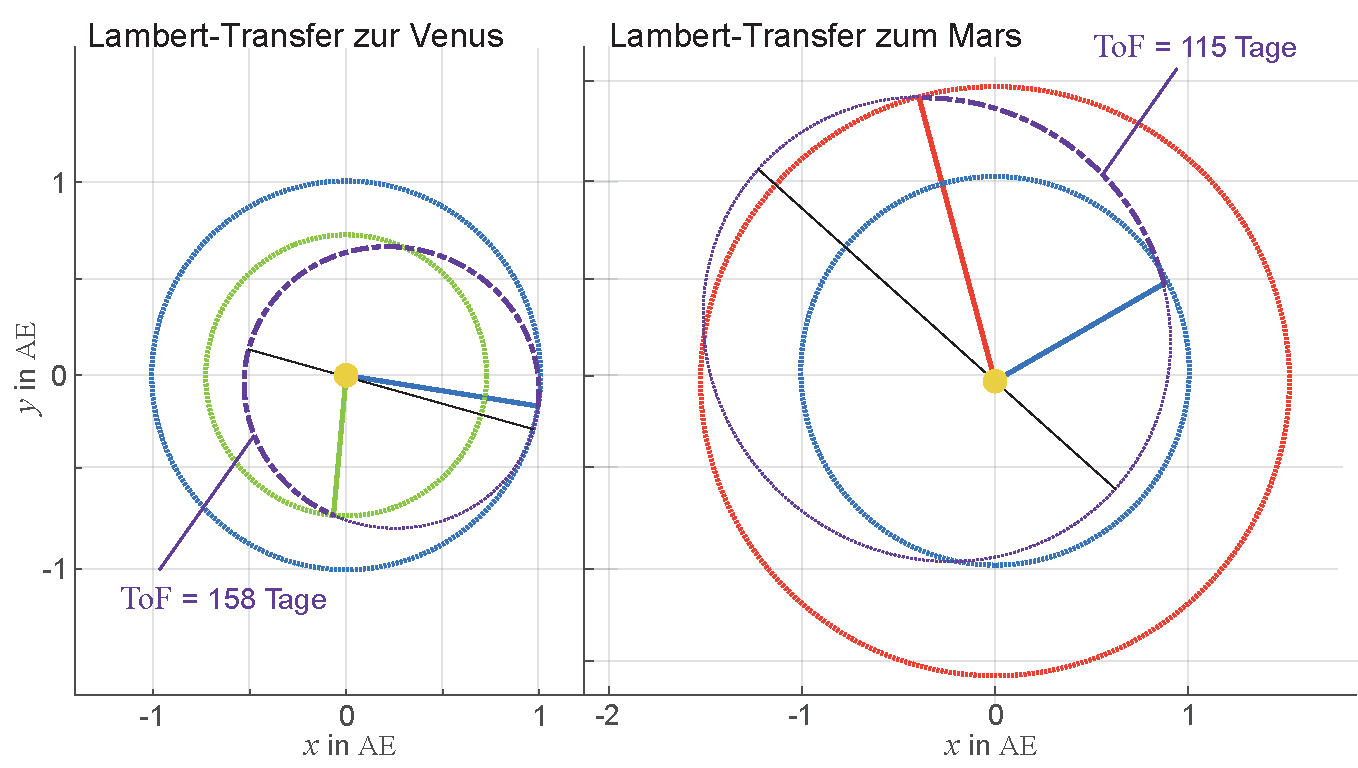
\includegraphics[width=\textwidth]{LambertTransferVenusMars.pdf} 
	\caption[L�sung des Lambert-Problems f�r Fl�ge zu Venus und Mars.]{L�sung des Lambert-Problems f�r Fl�ge zu Venus und Mars. Siehe \mscr~\mladynref{LambertProblem03.m}.}
	\label{abb:adyn_lambert_lsg06}
\end{figure}

\end{sol} 
\textcolor{blue} {$\rightarrow$ zur} \probref{adyn_manoevers5}.\\
\noindent\rule[1ex]{\textwidth}{0.5pt}  \newpage  \clearpage

%-----------------------------------------------------------------------------------------------------------

\begin{sol}{prob:adyn_manoevers6}\label{lsg:adyn_manoevers6} %�bung17
\textbf{Abfang ballistischer Raketen}\\

Die L�sung ist  im \mscr~\mladynref{LambertICBM.m} detailliert und mit ausf�hrlichen Kommentaren hinterlegt.
Die Vorgehensweise ist dabei wie folgt:
\begin{enumerate}[1.]
	\item Aus den gegebenen Werten f�r $\vec{R}$ und $\vec{V}$ der ICBM bestimmt man die Bahnparameter der ICBM. Wir verweisen auf \probref{adyn_orbits1}.
	\item Man berechnet mit diesen Bahnparametern �ber die Kepler-Gleichung \bzw die Methode mit den Gau�-Vektoren (PQR) (siehe \kap{hm_bahnen_hk_PQR}) den zeitlichen Verlauf der Trajektorie der ICBM und insbesondere den Punkt $\vec{R}(t_1+\mathrm{ToF})$, den diese nach $\mathrm{ToF}=\SI{30 }{\minute}$ errreicht. Wir erhalten:
\begin{align}
    \vec{R}(t_1+\mathrm{ToF})=[3930.7, 9762.2, 1583.3]\,\SI{}{\km}\,.
\end{align}
	\item F�r den Abf�nger gilt das Lambert-Problem mit $[\mathrm{P}_1,\mathrm{P}_2] = [\vec{r}(t_1), \vec{R}(t_1+\mathrm{ToF})]$.
	\item Man �berpr�ft, ob es �berhaupt eine L�sung geben kann. Dazu bestimmt man die minimale Flugzeit zu $t_\text{par} = \SI{16.0}{\minute}$ und die maximale Flugzeit zu $t_\text{m} = \SI{33.6}{\minute}$. Unsere $\mathrm{ToF}$ liegt dazwischen, es gibt also eine L�sung.
	\item Wir l�sen das Lambert-Problem wieder durch das in \probref{adyn_manoevers4} eingef�hrte Bisektionsverfahren und erhalten:
\begin{align}
    a=\SI{6130.7}{\km}\,,~~~\alpha = 2.9841\,,~~~\beta = 1.5418\,.
\end{align}
	\item Wir bestimmen mit diesen $a$, $\alpha$ und $\beta$ noch die notwendige Geschwindigkeit $\vec{v}_\text{trans}(t_1)$, die der Abf�nger am Punkt $\mathrm{P}_1$ haben muss, damit er auf die richtige Abfangbahn gelangt. Sie ergibt sich aus \eqref{eq:adyn_lambert08}zu:
\begin{align}
    \vec{v}_\text{trans}(t_1) &= (A+B)\,\vec{e}_c - (A-B)\,\vec{e}_1 = [2.16, 6.61, 1.13]\,\SI{}{\km\per\second}\, \\
		&\text{mit}\nonumber\\
		A &= \sqrt{\frac{G\,m_\text{E}}{4a}}\,\cot\frac{\alpha}{2}\,~~~~B = \sqrt{\frac{G\,m_\text{E}}{4a}}\,\cot\frac{\beta}{2}\,.\nonumber
\end{align}	
	\item Damit kann man sofort den erforderlichen Antriebsbedarf ermitteln, den man aufbringen muss, um den Abf�nger auf den richtigen Kurs zu bringen. Man erh�lt:
	\begin{align}
    \Delta \vec{v} &= \vec{v}_\text{trans}(t_1) - \vec{v}_1 = [4.66, 0.12,-1.37]\,\SI{}{\km\per\second}\,.		\\
		&\text{bzw}\nonumber\\
    \Delta v &= \SI{4.863}{\km\per\second}\,.
\end{align}	
	\item Zum Schlu� kann man aus $\vec{v}_\text{trans}(t_1)$ und $\vec{r}_1$ noch analog \probref{adyn_orbits1} die Bahnparameter der Abfangbahn berechnen und daraus mittels der Gau�-Vektoren-Methode (siehe \kap{hm_bahnen_hk_PQR}) die Trajektorie des Abf�ngers bestimmen, der sein Ziel nach genau 30 min erreicht (\figref{LambertAbfangICBM}).
\end{enumerate}

\begin{figure}[H]
	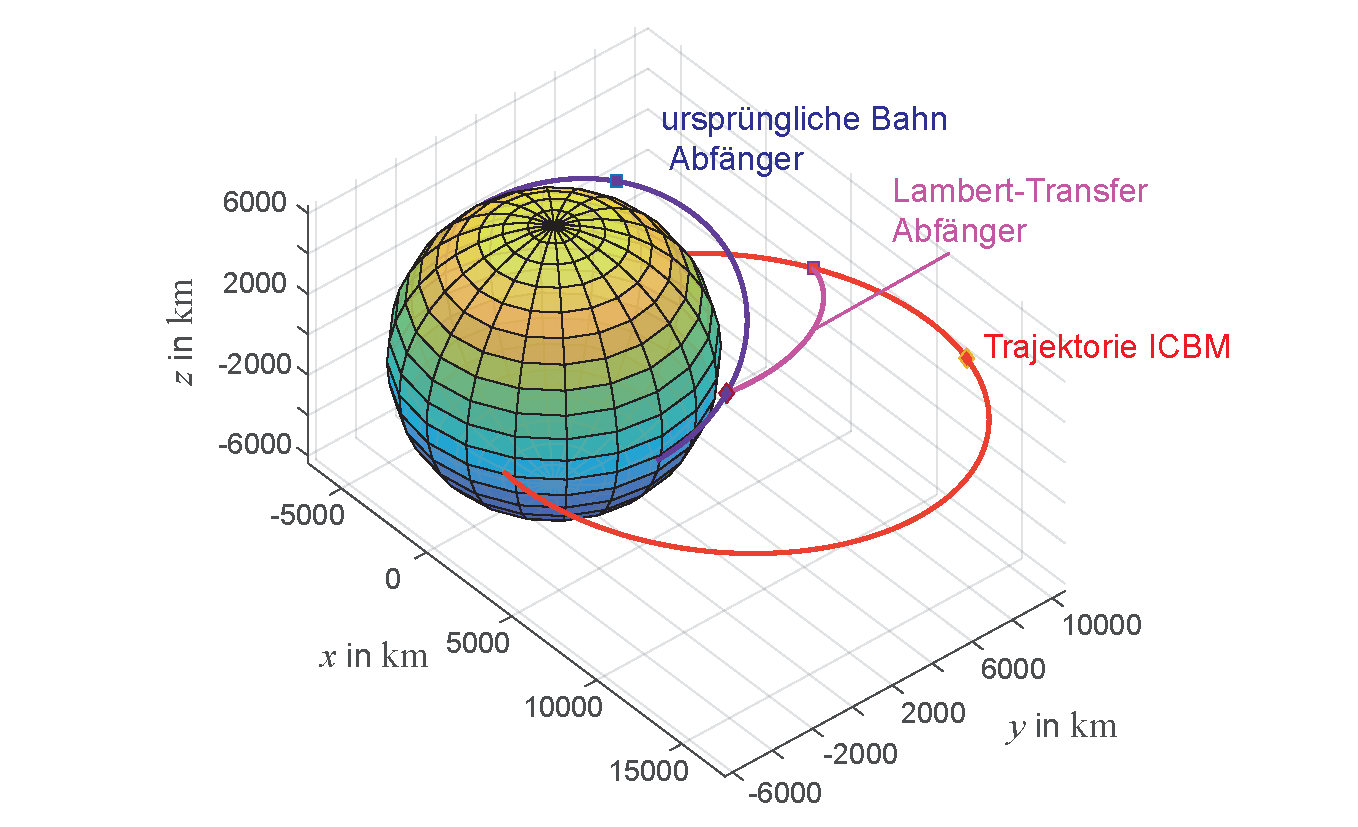
\includegraphics[width=\textwidth]{LambertAbfangICBM.pdf} 
	\caption[Abfang ballistischer Raketen.]{Abfang ballistischer Raketen. Dargestellt sind die Trajektorien der ICBM und des Abf�ngers mit und ohne $\Delta v$. Parameter siehe Text.}
	\label{abb:LambertAbfangICBM}
\end{figure}


\end{sol} 
\textcolor{blue} {$\rightarrow$ zur} \probref{adyn_manoevers6}.\\
\noindent\rule[1ex]{\textwidth}{0.5pt}  \newpage  \clearpage

%-----------------------------------------------------------------------------------------------------------

\begin{sol}{prob:adyn_manoevers7}\label{lsg:adyn_manoevers7} %�bung18
\textbf{Mondflug mit Ionenstrahltriebwerk}

\begin{itemize}
	\item
	Die Rechnungen sind im \mscr~\mladynref{Ionenantrieb02.m} ausgef�hrt und in \figref{IonenantriebExakt} dargestellt. Man sieht, dass die N�herung von \kap{adyn_kont_maneuver} zusammenbricht, wenn die Radius�nderung der Bahn per Umlauf gr��er wird.

\begin{figure}[H]
	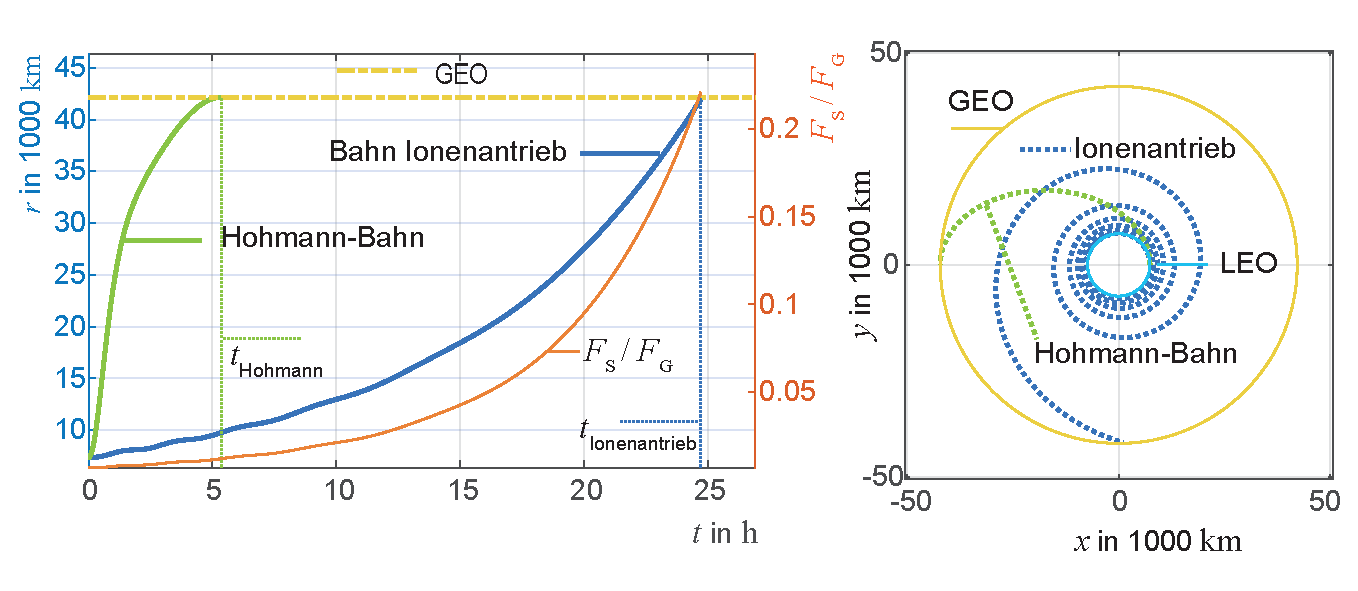
\includegraphics[width=\textwidth]{IonenantriebExakt.pdf} 
	\caption[Vergleich Hohmann-Transfer und Ionenantrieb.]{Vergleich Hohmann-Transfer und Ionenantrieb (LEO zu GEO), numerische L�sung der Bewegungsgleichung \eqref{eq:adyn_ionentr_01} f�r ein Triebwerk mit kontinuierlichem Schub. F�r den Ionenantrieb wurde ein konstanter Schub von $\SI{0.5}{\newton}$ angesetzt. Der Massenaussto� wurde bei der numerische Rechnung ber�cksichtigt.}
	\label{abb:IonenantriebExakt}
\end{figure}

	\item Die Rechnungen sind im \mscr~\mladynref{IonenantriebMond.m} ausgef�hrt. Dabei wurde die Triebwerksleistung entlang der Bahn linear so reduziert, dass sie bei der Entfernung, die dem Abstand des Lagrange-Punkts $\text{L}_1$ zwischen Erde und Mond entspricht, Null wird. Danach bewegt sich die Sonde allein im Gravitationsfeld des Mondes. Der Hohmann-Transfer wurde ebenfalls unter Ber�cksichtigung der Gravitationswirkung des Mondes berechnet.
Das Ergebnis der Rechnungen ist in der \figref{IonenantriebMoon} zu sehen.

\begin{figure}[H]
	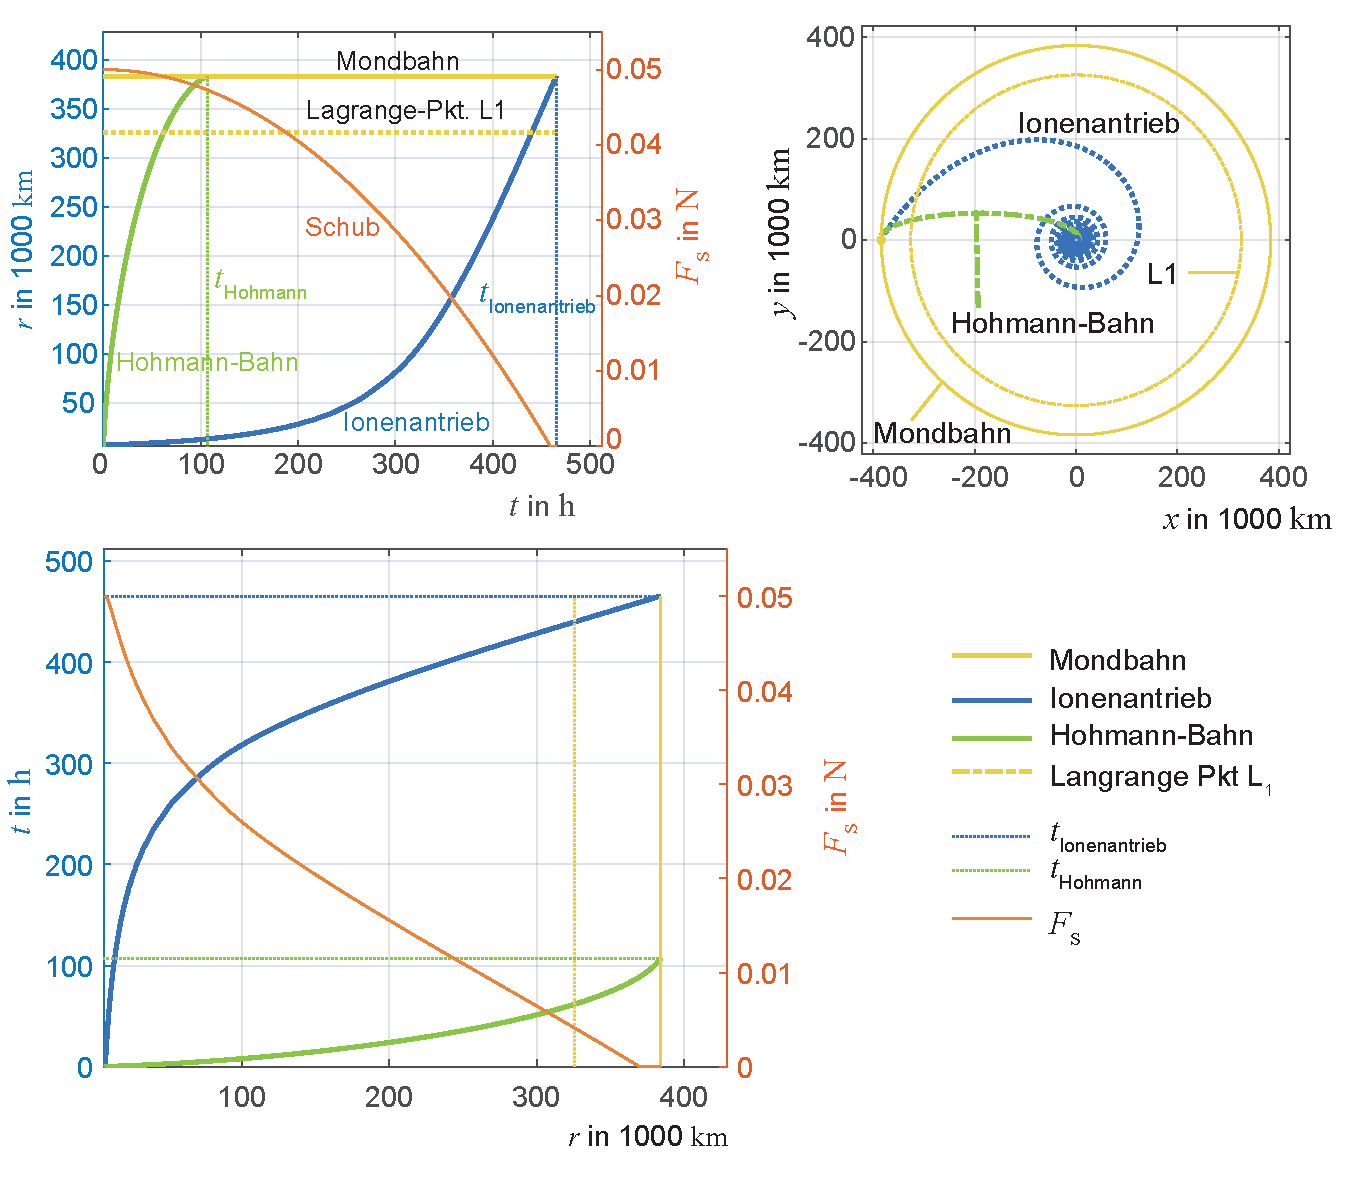
\includegraphics[width=\textwidth]{IonenantriebMoon.pdf} 
	\caption[Vergleich Hohmann-Transfer und Ionenantrieb zum Mond.]{Vergleich Hohmann-Transfer und Ionenantrieb zum Mond. F�r den Ionenantrieb wurde ein initialer Schub von $\SI{0.05}{\newton}$ der bis zum Gravitationsgleichgewicht zwischen Erde und Mond kontinuierlich reduziert wurde. Ebenso wurde der Massenaussto� bei der numerische Rechnung ber�cksichtigt.}
	\label{abb:IonenantriebMoon}
\end{figure}

\end{itemize}

\end{sol} 
\textcolor{blue} {$\rightarrow$ zur} \probref{adyn_manoevers7}.\\
\noindent\rule[1ex]{\textwidth}{0.5pt}  \newpage  \clearpage

%-----------------------------------------------------------------------------------------------------------

\begin{sol}{prob:adyn_SOI}\label{lsg:adyn_SOI} %�bung19
\textbf{Einflusssph�re - Sphere of Influence (SOI)}\\

Die Begriffe Hill-Sph�re\index{Hill-Sph�re} und Einflusssph�re\index{Einflusssph�re}\index{Sphere of Influence, SOI} adressieren zwei unterschiedliche Probleme:\\

\textit{Hill Sph�re:} Gegeben sind eine gro�e Masse $m_1$ (\zb die Sonne) und eine etwas kleinere Masse $m_2 < m_1$ (\zb die Erde) gegeben. Letztere bewegt sich um die gr��ere Masse. Es wird der Bereich gesucht, in dem f�r eine noch kleinere Masse $m_\text{M}$ (\zb der Mond) eine stabile Bahn um die kleine Masse ($m_2$) m�glich ist. Dieser Bereich wird Hill-Sph�re genannt. Die Berechnung der Hill-Sph�re hatten wir in \probref{hm_hill_sphere} ausf�hrlich behandelt und hatten dor mit $a$ als den Abstand zwischen den Massen $m_1$ und $m_2$ erhalten \eqref{eq:hm_moon_moon_lsg9}:
\begin{equation}
	r_\text{H} = a\,\sqrt[3]{\frac{1}{3}\frac{m_1}{m_2}} \,. \label{eq:adyn_hill_sphere_radius}:
\end{equation}

\textit{SOI:} Hier sind nun zwei relativ gro�e Massen $m_1, m_2$ gegeben (\zb Mars $m_1$ und Jupiter $m_2$ oder Sonne $m_2$ und Mars $m_1$ ) und eine sehr kleine Masse $m_\text{R}$ (\zb eine Raumsonde), die sich zwischen diesen beiden Massen bewegt. Es werden die Bereiche gesucht, in welchem jeweils eines der Zentren der Massen $m_1, m_2$ den Ursprung des Koordinatensystems bildet, welches f�r die Beschreibung der Bewegung der sehr kleinen Masse $m_\text{R}$  verwendet wird. In diesem Bereich muss dann f�r die Berechnung der Bewegung nur die Gravitationskraft der jeweiligen die SOI definierenden Masse $m_1$ oder $m_2$ ber�cksichtigt werden. Damit kann in der Astrodynamik bei interplanetaren Raumfl�gen die Trajektorie oft durch Aneinanderf�gen von Kepler-Bahn Abschnitten in den aufeinanderfolgenden SOI der einzelnen Planeten \bzw der Sonne (im interplanetaren Raum) n�herungsweise berechnet werden (sogenannte \textit{patched conic trajectories}.\\
Zur Herleitung der Beziehung f�r den Radius der SOI als Funktion der Massen  $m_1, m_2$ verwendet man zwei Referenzsysteme:
\begin{itemize}
	\item Zum einen erfolgt die Betrachtung der Bewegung der Raumsonde in einem Koordinaten\-system, dessen Ursprung im Zentrum der Masse $m_1$ liegt und ber�cksichtigt als Hauptwirkung nur die Gravitation der Masse $m_1$. Die Gravitationsbeschleunigung der gr��eren Masse $m_2$ wird in der Bewegungsgleichung als St�rgr��e eingef�hrt, im Prinzip als erste Abeitung.
	\item Dann betrachtet man die Bewegung der Raumsonde in dem \KOS, dessen Ursprung im Zentrum der Masse $m_2$ liegt und ber�cksichtigt als Hauptwirkung nur die Gravitation der Masse $m_2$. In der Bewegungsgleichung wird dann wiederum die Gravitationsbeschleunigung der Masse $m_1$ als St�rgr��e eingef�hrt.
\end{itemize}

\begin{figure}[H]
	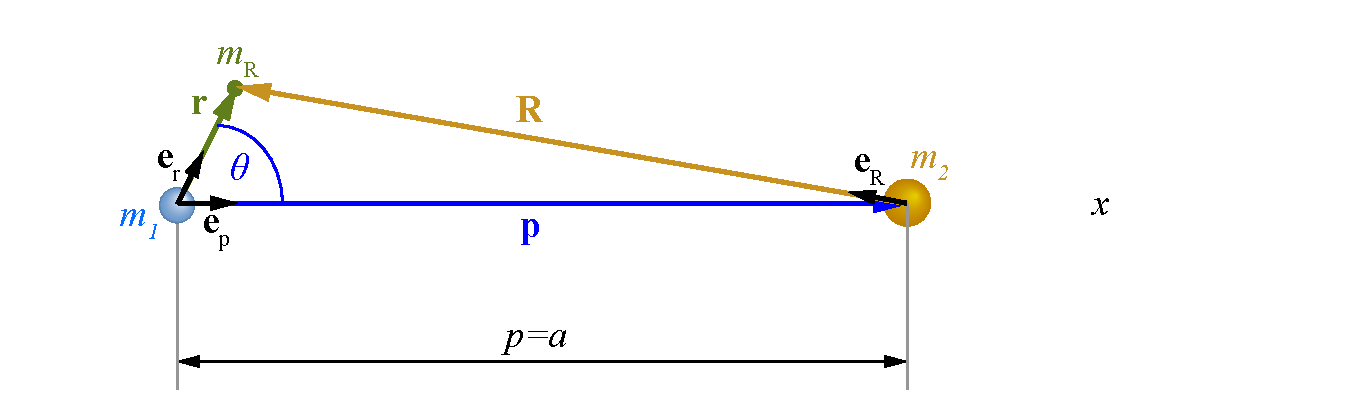
\includegraphics[width=\textwidth]{GeometrieHerleitungSOI.pdf} 
	\caption[Zur Herleitung der Einflusssph�re.]{Zur Herleitung der Einflusssph�re.}
	\label{abb:adyn_SOI01}
\end{figure}

Es ergeben sich folgende Bewegungsgleichungen (f�r $m_\text{R} \ll m_1,m_2$):\footnote{Die Herleitung wird als Zusatz�bung empfohlen, siehe auch \kap{hm_potentialtheorie} sowie \figref{adyn_SOI01}.}
\begin{subequations}
\begin{align}
    \ddot{\vec{r}} &= -G\,m_1\,\frac{\vec{r}}{r^3}-G\,m_2\,\lk\frac{\vec{p}}{p^3} + \frac{\vec{R}}{R^3}\rk\,,\\
    \ddot{\vec{R}} &= -G\,m_2\,\frac{\vec{R}}{R^3}-G\,m_1\,\lk\frac{\vec{r}}{r^3} - \frac{\vec{p}}{p^3}\rk\,.
\end{align}    \label{eq:adyn_SOI01}
\end{subequations}

Diese Gleichungen k�nnen geschrieben werden als:
\begin{subequations}
\begin{align}
     \ddot{\vec{r}} &= \vec{a}_{\text{H},1}^{\lk 1 \rk} + \vec{a}_{\text{S},2}^{\lk 1 \rk}\,, \\
     \ddot{\vec{R}} &= \vec{a}_{\text{H},2}^{\lk 2 \rk} + \vec{a}_{\text{S},1}^{\lk 2 \rk} \,,
\end{align} \label{eq:adyn_SOI02}
\end{subequations}

worin in $\vec{a}_{\text{H,S},i}^{\lk j \rk}$ der Index $j$ das KOS-System des jeweiligen Planeten bezeichnet und H und S f�r die Hauptgravitations- \bzw St�rbeschleunigung stehen. Letztere wird hervorgerufen jeweils durch die Masse $m_i$ ($i=1,2$). Die Beschleunigungen k�nnen mit den Einheitsvektoren $\vec{e}_\text{r},\, \vec{e}_\text{R}$ und $\vec{e}_\text{p}$aus \figref{adyn_SOI01} beschrieben werden durch:

\begin{subequations}
\begin{align}
   \vec{a}_{\text{H},1}^{\lk 1 \rk} &= -\frac{G\,m_1}{r^2}\,\vec{e}_\text{r}\,,\label{eq:adyn_SOI03a} \\ 
    \vec{a}_{\text{H},2}^{\lk 2 \rk} &= -\frac{G\,m_2}{R^2}\,\vec{e}_\text{R}\,, \label{eq:adyn_SOI03b} \\
    \vec{a}_{\text{S},2}^{\lk 1 \rk} &= +\,G\,\frac{m_2}{p^2}\,\sum\limits_{k=1}^\infty \lk \frac{r}{p}\rk^k\lek {\PL {k+1}}'\lk  \cos\theta\rk\,\vec{e}_\text{p} - {\PL {k}}'\lk\cos\theta\rk\,\vec{e}_\text{r} \rek\,, \label{eq:adyn_SOI03c} \\ 
    \vec{a}_{\text{S},1}^{\lk 2 \rk}&= +\,G\,\frac{m_1}{r^2}\,\lek \lk \frac{r}{p} \rk^2\,\vec{e}_\text{p} - \vec{e}_\text{r} \rek\,, \label{eq:adyn_SOI03d}
\end{align} \label{eq:adyn_SOI03}
\end{subequations}  

worin $\PL k$ die im \kap{hm_potentialtheorie} eingef�hrten Legendre-Polynome sind (\cite{Andrews2003}) und ${\PL k}'$ deren erste Ableitungen. 
Die Gleichungen sind direkt aus \eqref{eq:adyn_SOI01} ablesbar. Lediglich Gleichung \eqref{eq:adyn_SOI03b} erfordert eine Nebenrechnung. Sie ergibt sich aus der Definition der Legendre-Polynome und der Nutzung der verschiedenen Beziehungen zwischen den Ableitungen und den Rekursionsformeln (\cite{Riley2006, Andrews2003}). 
Wir bilden nun die Verh�ltnisse von Hauptbeschleunigung zu St�rbeschleunigung im jeweiligen \KOS. Wir dividieren dazu \eqref{eq:adyn_SOI03d} durch \eqref{eq:adyn_SOI03b} und finden:
\begin{align}
    \frac{ \vec{a}_\text{S1}^{\lk 2\rk}}{ \vec{a}_\text{H2}^{\lk 2\rk}} = \frac{m_1}{m_2}= \frac{1-2\,\lk\frac{r}{p}\rk\,\cos\theta + \lk\frac{r}{p}\rk^2}{\lk\frac{r}{p}\rk^2}\,\sqrt{\lek 1-2\,\lk\frac{r}{p}\rk^2\,\cos\theta + \lk\frac{r}{p}\rk^4\rek} \,.\label{eq:adyn_SOI04}
\end{align}
Analog erh�lt man durch Division von \eqref{eq:adyn_SOI03c} durch \eqref{eq:adyn_SOI03a}:
\begin{align}
    \frac{\vec{a}_{\text{S},2}^{\lk 2\rk}}{\vec{a}_{\text{H},1}^{\lk 2\rk}} = \frac{m_1}{m_2}\,\lk \frac{r}{p} \rk^3 \, \sqrt{\lek 1+3\cos^2\theta \rek} + \mathcal{O}\lk\frac{r}{p}^4\rk \,, \label{eq:adyn_SOI05}
\end{align}
wobei wir hier wegen $r \ll p$ alle Terme mit Potenzen von $\lk \frac{r}{p} \rk^n$, $n>3$ vernachl�ssigen. Die Gleichungen dr�cken das Verh�ltnis von St�rbeschleunigung zu Hauptbeschleunigung im jeweiligen Bezugssystem aus.\\
Gleichsetzen von \eqref{eq:adyn_SOI04} mit \eqref{eq:adyn_SOI05} bedeutet, dass die St�rungs- und Hauptbeschleunigungen an einem Ort im Abstand $r_\text{SOI} $ von dem jeweiligen Zentrum des \KOS im gleichen Verh�ltnis zueinander stehen. Man erh�lt dann eine diesen Abstand unter der Annahme $r/p \ll 1$: 
\begin{align}
    \frac{r_\text{SOI}}{p} &= \sqrt[5]{\frac{m_1{}^2}{m_2{}^2}}\,\underbrace{\lk 1+3\cos^2\theta\rk^{-\frac{1}{10}}}_{\leq 1.148}~~\rightarrow ~~~ \frac{r_\text{SOI}}{p} \approx \lk \frac{m_1}{m_2}\rk^{\frac{2}{5}}\,. \label{eq:adyn_SOI06}
\end{align}
Der Radius einer SOI h�ngt somit vom Abstand $p$ beider Massen und dem Verh�ltnis (hoch $2/5$) der beiden Massen ab. Tabelle \ref{tab:adyn_SOI01} zeigt die Radien der SOI der Planeten unseres Sonnensystems im Vergleich zu den Radien der Hill-Sph�re \eqref{eq:adyn_hill_sphere_radius}:
\begin{table}[ht]
		\begin{center}
    \begin{tabular}{|C{1.5cm}|C{2.75cm}|C{2.75cm}|C{2.75cm}|C{2.75cm}|}
    \hline
    \rule{0pt}{3pt}& & &&  \\
      Planet (Masse $m_1$) & Gro�e Halbachse\linebreak zur Sonne \linebreak (Masse $m_2$)\linebreak $\lk\SI{}{\km}\rk$ & Massenverh�ltnis Planet/Sonne \linebreak $m_1/m_2$& Radius der SOI \linebreak  $\lk\SI{}{\km}\rk$ \linebreak \linebreak \eqref{eq:adyn_SOI_radius} &  Radius der Hill-Sph�re  \linebreak  $\lk\SI{}{\km}\rk$ \linebreak \linebreak \eqref{eq:adyn_hill_sphere_radius} \\
    \rule{0pt}{3pt}&& &&  \\
    \hline
    \rule{0pt}{3pt}&& &&   \\
    \rule{0pt}{6pt} Merkur &\SI{57.9e6}{}&$\SI{0.166e-6}{}$ & $\SI{112000e06}{}$& $\SI{2.206e05}{}$\\
    \rule{0pt}{3pt}&& &&   \\
    \rule{0pt}{6pt} Venus &\SI{108.2e6}{}&$\SI{2.450e-6}{}$ & $\SI{616350e06}{}$& $\SI{1.010e+06}{}$\\
    \rule{0pt}{3pt}&& &&   \\
    \rule{0pt}{6pt} Erde & \SI{149.6e6}{}&$\SI{3.002e-6}{}$ & $\SI{924510e06}{}$& $\SI{1.496e+06}{}$\\
    \rule{0pt}{3pt}&& &&   \\
    \rule{0pt}{6pt} Mars &\SI{227.9e6}{}&$\SI{0.323e-6}{}$ & $\SI{577230e06}{}$& $\SI{1.084e+06}{}$\\
    \rule{0pt}{3pt}&& &&   \\
    \rule{0pt}{6pt} Jupiter &\SI{778.6e6}{}&$\SI{954.490e-6}{}$ & $\SI{48219000e06}{}$& $\SI{5.315e+07}{}$\\
    \rule{0pt}{3pt}&& &&   \\
    \rule{0pt}{6pt} Saturn &\SI{1433.5e6}{}&$\SI{285.641e-6}{}$ & $\SI{54793000e06}{}$& $\SI{6.546e+07}{}$\\
    \rule{0pt}{3pt}&& &&   \\
    \rule{0pt}{6pt} Uranus &\SI{2872.5e6}{}&$\SI{43.651e-6}{}$ & $\SI{51791000e06}{}$& $\SI{7.013e+07}{}$\\
    \rule{0pt}{3pt}&& &&   \\
    \rule{0pt}{6pt} Neptun &\SI{4495.1e6}{}&$\SI{51.295e-6}{}$ & $\SI{86451000e06}{}$& $\SI{1.158e+08}{}$\\
    \rule{0pt}{3pt}&& &&   \\
    \hline
    \end{tabular} 
		\end{center}
		\caption{Vergleich Radien der SOI mit dem Hill-Sph�re f�r die Planeten unseres Sonnensystems.}
		\label{tab:adyn_SOI01}
\end{table}

Im letzten Schritt in \eqref{eq:adyn_SOI06} haben wir die $\theta$-Abh�ngigkeit vernachl�ssigt. Ber�cksichtigt man diese, so ergibt sich ein oblater Sph�roid anstelle einer Einflusssph�re (Sphere of Influence). In den meisten F�llen reicht die Kugelbetrachtung aber aus, man kann also schreiben:
\begin{align}
	r_\text{SOI} = a\,\sqrt[5]{\lk \frac{m_1}{m_2}\rk^2} \,, \label{eq:adyn_SOI_radius}
\end{align}
worin a der Abstand zwischen den beiden Massen (\ia gleich der gro�en Halbachse von $m_1$ um $m_2$) ist.\\
Man wird also immer dann, wenn sich die Raumsonde in geringerem Abstand als $r_\text{SOI}$  von der Masse $m_1$ befindet, die Bewegung als Zweik�rperproblem mit den Massen $m_1,\,m_\text{R}$ behandeln k�nnen, bei Abst�nden gr��er als $r_\text{SOI}$ als Zweik�rperproblem mit den Massen $m_2,\,m_\text{R}$.\\

\end{sol} 
\textcolor{blue} {$\rightarrow$ zur} \probref{adyn_SOI}.\\
\noindent\rule[1ex]{\textwidth}{0.5pt}  \newpage  \clearpage

%-----------------------------------------------------------------------------------------------------------

\begin{sol}{prob:adyn_swingby01}\label{lsg:adyn_swingby01} %�bung20
\textbf{Gravity-Assist-Man�ver - Analytische L�sung}\\

Wir beginnen mit:
\begin{subequations}
\begin{align}
        \vec{v}_1{}' &= \vec{v}_1 - \vec{v}_\text{P} \,, \label{eq:adyn_lsgswingby01a} \\
        v_1{}'^2     &= v_1{}^2 + v_\text{P}{}^2 - 2\,v_1{}'\,v_\text{P}\,\cos\gamma_1{}'\,, \label{eq:adyn_lsgswingby01b} \\
        \vec{v}_2{}  &= \vec{v}_2{}' + \vec{v}_\text{P} \,, \label{eq:adyn_lsgswingby02a} \\
        v_2{}^2      &= v_2{}'^2 + v_\text{P}{}^2 + 2\,v_2{}'\,v_\text{P}\,\cos\beta_2{}' \,, \label{eq:adyn_lsgswingby02b} \\
        v_1{}'       &= v_2{}'= v_\infty \,. \label{eq:adyn_lsgswingby02c} 
\end{align} %\label{eq:adyn_lsgswingby02} 
\end{subequations}
F�r die weitere numerische Auswertung lassen sich aus \eqref{eq:adyn_swingby01}, \eqref{eq:adyn_swingby03} und \figref{adyn_swingby01} durch Anwendung des Kosinussatzes \bzw geometrische �berlegungen aus der Streuhyperbel noch einige n�tzliche Beziehungen, \zb zwischen dem Winkel $\beta_2{}'$ und dem Streuwinkel $\vartheta'$ sowie f�r den Winkel $\varphi'$ gewinnen:
\begin{subequations}
\begin{align}
        \beta_2{}' &= \beta_1{}' -\vartheta' = \beta_1{}' + 2\varphi' - 180\degree \label{eq:adyn_lsgswingby03a} \\
        \cos\beta_2{}' &= \cos\,\beta_1{}'\,\lk 1-2\cos^2\varphi'\rk + 2\cos\varphi'\,\sqrt{1-\cos^2\varphi'}\,\sqrt{1-\beta_1'{}^2} \label{eq:adyn_lsgswingby03b} \\
        \cos\beta_1{}' &= \frac{{v_1{}}^2+v_\text{P}{}^2-{v_1{}'}^2}{2\,v_1\,v_\text{P}} \label{eq:adyn_lsgswingby03c}
\end{align}%\label{eq:adyn_lsgswingby03} 
\end{subequations}
Die Gr��e $\cos\varphi'$ k�nnen wir ebenfalls aus \figref{adyn_swingby01} mit der Hyperbelgleichung durch
\begin{align}
    \cos\varphi' &= \frac{1}{1+ (r_\text{per}\,v_1{}'^2)/(G\,m_\text{P})} = -\frac{1}{e}\,\label{eq:adyn_lsgswingby04} 
\end{align}
ausdr�cken.

\begin{nebenrechnungNeu} {} \\
Der Winkel $\varphi'$ h�ngt mit dem asymptotischen Grenzwinkel $\theta_\infty{}'$ der Hyperbel wie folgt zusammen:
\begin{align}
    \theta_\infty{}' = -\frac{1}{e} = + \cos\lk 180\degree-\varphi'\rk = - \cos\varphi' \label{eq:adyn_lsgswingby05} 
\end{align}
Die Exzentrizit�t ist nach \eqref{eq:hm_relations2} gegeben durch
\begin{align}
    e= \sqrt{1+\frac{2\,H\,L^2}{\mu_\text{P}{}^2}} = \sqrt{1+\frac{2L^2}{\mu_\text{P}{}^2}\,\frac{v_1{}'^2}{2}} = \sqrt{1 + \frac{b^2\,v_1{}'^4}{\mu_\text{P}^2}}\,, \label{eq:adyn_lsgswingby06} 
\end{align}
wobei wir $H = v_1{}'^2/2$ f�r $r\to \infty$ und $L_\infty = b\,v_1{}' = b\,v_2{}' = b\, v_\infty$ f�r $r\to \infty$ benutzt haben.\\
Wegen der Drehimpulserhaltung k�nnen wir $L_\infty$ durch $L_\text{per} = r_\text{per}\,v_\text{per}{}'$ am Perizentrum ersetzen und benutzen dabei den \textit{vis-viva}-Satz \eqref{eq:hm_vis-viva}, womit wir erhalten:
\begin{align}
    L = b\,v_1{}' = r_\text{per}\,v_\text{per}{}'~~~\text{und}~~~
    \frac{v_1{}'}{2}^2 = \frac{v_\text{per}{}'^2}{2} - \frac{\mu_\text{P}}{r_\text{per}}\,.\label{eq:adyn_lsgswingby07} 
\end{align}
\end{nebenrechnungNeu}

\newpage
Mit den Beziehungen in \eqref{eq:adyn_lsgswingby07} k�nnen wir in \eqref{eq:adyn_lsgswingby06} den Streuparameter $b$ eliminieren und erhalten aus \eqref{eq:adyn_lsgswingby02b} mit \eqref{eq:adyn_lsgswingby05} �ber \eqref{eq:adyn_lsgswingby03b} schlie�lich die heliozentrische Geschwindigkeit des Raumschiffs $v_2$ beim Verlassen der Einflusssph�re des Gravity-Assist-Planeten am Punkt $\text{P}_2$:
\begin{subequations}
    \begin{align}
        v_2{}^2 = v_1{}^2 - \frac{2\,C_1}{C_2{}^2} + \frac{4\,v_1{}'\,v_\text{P}}{C_2}\,\sqrt{1-\frac{1}{C_2{}^2}}\,\sqrt{1-\lk\frac{C_1}{2\,v_1{}'\,v_\text{P}}\rk^2}\label{eq:adyn_lsgswingby08a}
    \end{align}
    mit 
    \begin{align}
        C_1 &= v_1{}^2 - v_\text{P}^2 - v_1{}'^2 \label{eq:adyn_lsgswingby08b}\,,\\
        C_2 &= 1+\frac{r_\text{per}}{\mu_\text{P}}\,v_1{}'{}^2 \label{eq:adyn_lsgswingby08c}\,,\\
        v_1{}'&= \sqrt{v_1{}^2 +v_\text{P}{}^2 - 2\,v_1\,v_\text{P}\,\cos\gamma_1}\,.\label{eq:adyn_lsgswingby08d}
    \end{align}%\label{eq:adyn_lsgswingby08}
\end{subequations}
Wir haben $v_2(r_\text{per},\gamma_1)$ in \figref{adyn_lsgswingby01} dargestellt.

\begin{figure}[H]
	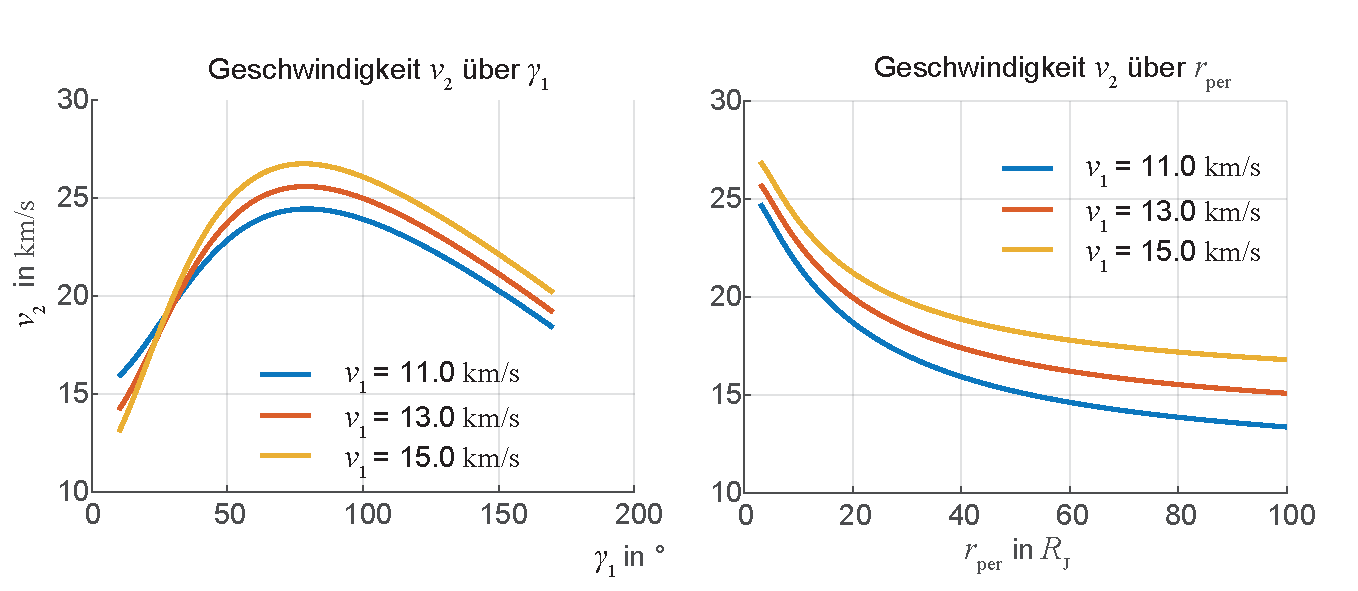
\includegraphics[width=\textwidth]{GravityAssistAnalytisch.pdf} 
	\caption[Gravity-Assist-Man�ver (Analytisch L�sung).]{Gravity-Assist-Man�ver (Analytisch L�sung).}
	\label{abb:adyn_lsgswingby01}
\end{figure}

Zum Schluss wollen wir noch den maximal m�glichen Energiegewinn bei einem Gravity-Assist-Man�ver berechnen. Dieser ergibt sich zu
\begin{align}
    \Delta H &= \frac{1}{2}\,v_2{}^2 - \frac{m_\text{S}\,G}{r_1-r_\text{per}} - \lk \frac{1}{2}\,v_1{}^2 - \frac{m_\text{S}\,G}{r_1-r_\text{per}}\rk \approx \frac{1}{2}\,\lk v_2{}^2 - v_1{}^2\rk \,.\label{eq:adyn_lsgswingby09}
\end{align}
Der Energiegewinn h�ngt also bei vorgegebenen $r_\text{per}$ von zwei Parametern ab:\\
$v_1{}'$ (\bzw. $v_1$)\, und $\beta_1{}'$ (\bzw $\gamma_1$).
Tr�gt man $\Delta H$ �ber $\beta_1{}'$ und $v_1{}'$ auf, so findet man ein Maximum bei $\beta_1{}' = 2\pi/3=120\degree$ und 
	\[v_1{}' = \sqrt{\frac{\mu_\text{P}}{r_\text{per}}}\,,
\]
Damit kann man mit den bekannten Gr��en $m_\text{P}$, $r_\text{per}$ (wir nehmen $r_\text{per} \approx 5\,R_\text{P}$ an) und $v_\text{P}$ die notwendig Anfluggeschwindigkeit $v_\text{1,opt}$ bestimmt, die den maximalen Energiegewinn bringt. Die Rechnungen sind im Detail \mscr{} \mladynref{GravityAssistAnalytik.m} ausgef�hrt. 

Der Energiegewinn $\Delta H(v_1{}', \beta_1{}')$ \bzw $\Delta H(v_1{}, \gamma_1{})$ ist in \figref{adyn_lsgswingby02a} dargestellt:

\begin{figure}[H]
	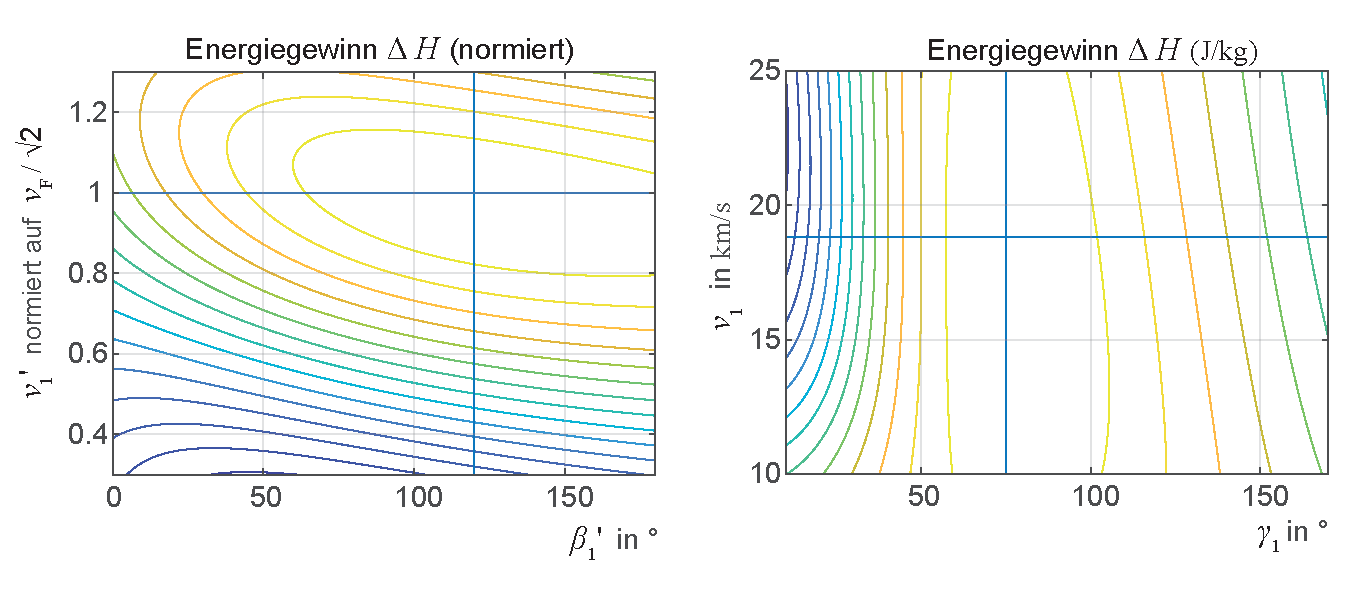
\includegraphics[width=\textwidth]{GravityAssistEnergiegewinn.pdf} 
	\caption[Gravity-Assist-Man�ver - Energiegewinn.]{Gravity-Assist-Man�ver - Energiegewinn am Beispiel des Flugs einer Raumsonde um den Jupiter.  Parameter: $r>_\text{per} = 5\,R_\text{J}$.}
	\label{abb:adyn_lsgswingby02a}
\end{figure}

\end{sol} 
\textcolor{blue} {$\rightarrow$ zur} \probref{adyn_swingby01}.\\
\noindent\rule[1ex]{\textwidth}{0.5pt}  \newpage  \clearpage
%
%%-----------------------------------------------------------------------------------------------------------

\begin{sol}{prob:adyn_swingby03}\label{lsg:adyn_swingby03} %�bung21
\textbf{Gravity-Assist-Man�ver - Simulation}\\

Die Simulation des Swing-By ist im \mscr{} \mladynref{GravityAssistSimulation.m} ausgef�hrt, die Resultate f�r ein Beispiel am Jupiter in \figref{adyn_lsgswingby02}.\\

\begin{figure}[H]
	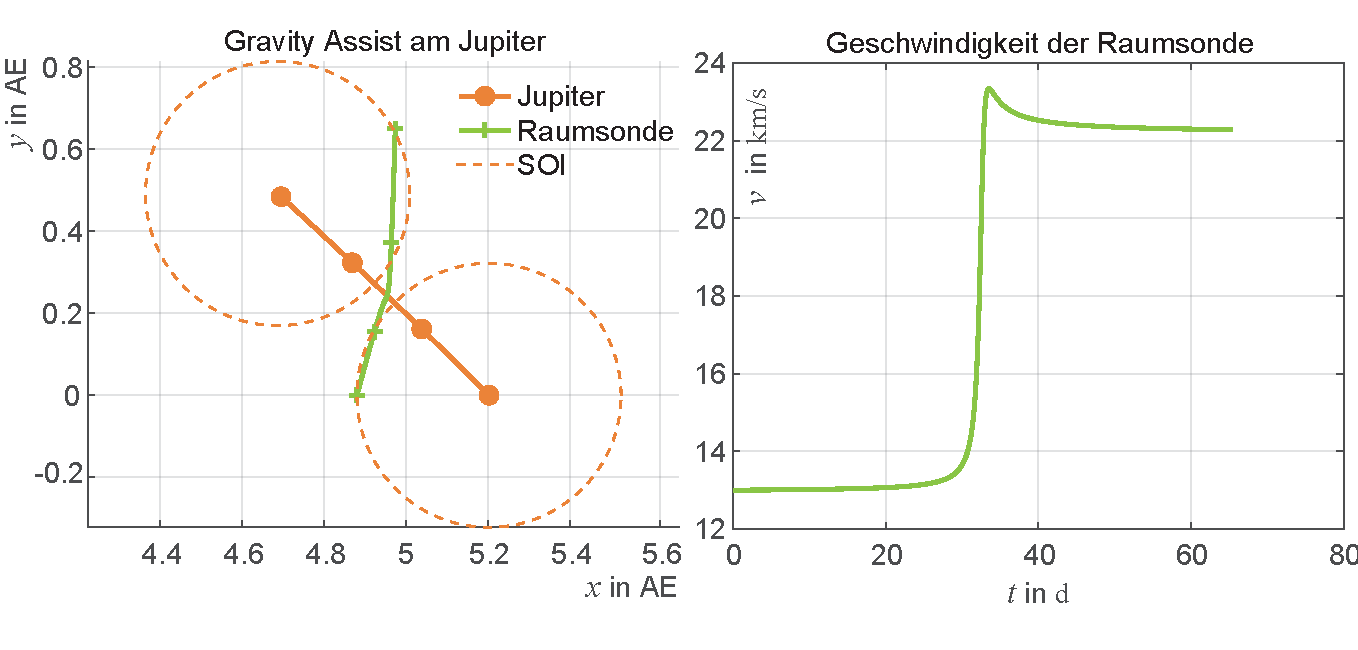
\includegraphics[width=\textwidth]{GravityAssistSimulation.pdf} 
	\caption[Gravity-Assist-Man�ver Simulation.]{Ergebnisse der Gravity-Assist-Man�ver Simulation im heliozentrischen \KOS am Beispiel des Flugs einer Raumsonde um den Jupiter.  Parameter: $v_1 = \SI{13.0}{\km\per\second}$, $\gamma_1 = 75\degree$.}
	\label{abb:adyn_lsgswingby02}
\end{figure}

\end{sol} 
\textcolor{blue} {$\rightarrow$ zur} \probref{adyn_swingby03}.\\
\noindent\rule[1ex]{\textwidth}{0.5pt}  \newpage  \clearpage

%-----------------------------------------------------------------------------------------------------------
\newpage 
\subsection{�bungen zu Rendezvous im Weltall}

\begin{sol}{prob:adyn_rendezvous01}\label{lsg:adyn_rendezvous01} %�bung22
\textbf{Rendezvous ISS und Raumtransporter}\\

Wir wollen zun�chst die Beziehungen \eqref{eq:adyn_rendez23} und \eqref{eq:adyn_rendez24} aus \kap{adyn_rendezvous} herleiten, die wir f�r unsere \matlab-
Programmierung gut verweenden k�nnen. Wir starten von der Darstellung \eqref{eq:adyn_rendez23}:
\begin{nebenrechnungNeu} {Clohessy-Wiltshire-Gleichungen}
\begin{align}
\begin{split}
    \omega\,x &= \lk 6 \omega\, y_0 + 4\dot{x}_0\rk\,  \sin \omega t + 2 \dot{y}_0 \, \cos \omega t + \omega t \, \lk -6 \omega\,  y_0 - 3 \dot{x}_0\rk  + \omega\,  \lk x_0 - 2 \dot{y}_0\rk\,,  \\
    \omega \, y &= \lk \dot{y}_0\rk \,  \sin \omega t + \lk -3 \omega \, y_0 - 2 \dot{x}_0\rk \,  \cos \omega t + \omega \, \lk 4 y_0 + 2 \dot{x}_0\rk  \, ,\\
    \omega \, z &= \dot{z}_0\, \sin \omega t + \omega\,  z_0 \, \cos \omega t +0
\end{split}\label{eq:adyn_CWEq_01}
\end{align}

Umordnung nach $\dot{x}_0, \dot{y}_0, \dot{z}_0$ und $x = y = z = 0$:

\begin{align}
\begin{split}
    \begin{pmatrix} 0 \\ 0 \\ 0 \end{pmatrix} =\,
    &\underbrace{\begin{pmatrix} 4 \sin \omega t - 3 \omega t & 2 \cos \omega t - 2 & 0 \\
    -2 \cos \omega t + 2 & \sin \omega t & 0 \\
    0 & 0 & \sin \omega t 
    \end{pmatrix} }_{\substack{\hat{A}}}
    \begin{pmatrix} \dot{x}_0 \\ \dot{y}_0 \\ \dot{z}_0 \end{pmatrix} 
    \\ &+ \underbrace{\begin{pmatrix} 6 \omega \,y_0\, \sin \omega t - 6 \omega^2 t\,y_0 + \omega x_0 \\
    -3 \omega \,y_0\, \cos \omega t + 4 \omega\, y_0 \\
    \omega\, z_0\, \cos \omega t 
    \end{pmatrix}}_{\substack{-\hat{B}}}
\end{split}\label{eq:adyn_CWEq_02}
\end{align}
\begin{align}
    -\hat{B} &= \omega \, 
    \begin{pmatrix}
        6 y_0\,\sin \omega t - 6 \omega t \,y_0 + x_0 \\ 
        -3 y_0\, \cos \omega t + 4 y_0 \\ 
        z_0\, \cos \omega t 
    \end{pmatrix} \label{eq:adyn_CWEq_03}\\
    \rightarrow \quad \hat{B} &= \omega \,
    \begin{pmatrix}
        -6 y_0 \,\sin \omega t + 6 \omega t\, y_0 - x_0 \\ 
        3 y_0\, \cos \omega t - 4 y_0 \\ 
        -z_0\, \cos \omega t 
    \end{pmatrix} \label{eq:adyn_CWEq_04}\\
  \rightarrow\quad  \hat{B} &=      \hat{A} \hat{X}\nonumber\\
    \rightarrow\quad \hat{X} &= 
    \begin{pmatrix} 
        \dot{x}_0 \\ 
        \dot{y}_0 \\ 
        \dot{z}_0 
    \end{pmatrix} 
    = \hat{A}^{-1}\, B\label{eq:adyn_CWEq_05}
\end{align}
\subsubsection*{Cramersche Regel}
\begin{align}
    \dot{x}_0 &= \frac{\det \hat{A}_x}{\det \hat{A}}, \quad
    \dot{y}_0 = \frac{\det \hat{A}_y}{\det \hat{A}}, \quad
    \dot{z}_0 = \frac{\det \hat{A}_z}{\det \hat{A}}\label{eq:adyn_CWEq_06}
\end{align}
\begin{align}
    \det \hat{A} &= 
    \begin{vmatrix}
        \lk 4 \sin \omega t - 3 \omega t \rk & -2\, \lk 1 - \cos \omega t \rk & 0 \\
        +2 \,\lk 1 - \cos \omega t \rk & \sin \omega t & 0 \\
        0 & 0 & \sin \omega t
    \end{vmatrix} \label{eq:adyn_CWEq_07}
\end{align}
\begin{align*}
    &= \lk 4 \sin \omega t - 3 \omega t \rk\, \sin^2 \omega t + 4 \sin \omega t \,\lk 1 - \cos \omega t \rk^2\\
    &= \sin \omega t \,
    \lk 4 \sin^2 \omega t - 3 \omega t \,\sin \omega t + 4 + 4 \cos^2 \omega t - 8 \cos \omega t \rk\\
    &= \sin \omega t \,
    \lek 8 \,\lk 1 - \cos \omega t \rk - 3 \omega t\, \sin \omega t \rek
\end{align*}
\begin{align}
    \det \hat{A}_z &=
    \begin{vmatrix}
         4 \sin \omega t - 3 \omega t & -2 \,\lk 1 - \cos \omega t \rk & -6 \omega \,y_0\, \sin \omega t + 6 \omega^2 t\, y_0 - \omega \,x_0 \\
        2 \,\lk 1 - \cos \omega t \rk & \sin \omega t & -3 \omega \,y_0\, \cos \omega t - 4 \omega \,y_0 \\
        0 & 0 & -\omega \,z_0\, \cos \omega t
    \end{vmatrix}\\
    &= -\lk 4 \sin \omega t - 3 \omega t \rk \,\sin \omega t \,\omega \,z_0 \,\cos \omega t - 4 \omega \,z_0 \,\cos \omega t \,\lk 1 - \cos \omega t \rk^2\nonumber\\
    &= -\cos \omega t \,\omega \,z_0 \,
    \lk 4 \sin^2 \omega t - 3 \omega t \,\sin \omega t + 4 + 4 \cos^2 \omega t - 8 \cos \omega t \rk \nonumber\\
    &= -\cos \omega t \,\omega \,z_0 \,
    \lek 8 \,\lk 1 - \cos \omega t \rk - 3 \omega t \,\sin \omega t \rek \nonumber\\
    \rightarrow \quad \dot{z}_0 &= - \frac{\cos \omega t\, \omega\, z_0}{\sin\omega t} = -\frac{\omega\,z_0}{\tan\omega t}\label{eq:adyn_CWEq_09}
\end{align}
\begin{align}
    \det \hat{A}_x &=
    \begin{vmatrix}
        6 \omega \,y_0\, \sin \omega t - 6 \omega^2 \,t \,y_0 + \omega \,x_0 & -2 \,\lk 1 - \cos \omega t \rk & 0 \\
        -3 \omega\, y_0\, \cos \omega t + 4 \omega\, y_0 & \sin \omega t & 0 \\
        \omega\, z_0\, \cos \omega t & 0 & \sin \omega t
    \end{vmatrix}\label{eq:adyn_CWEq_10}
\end{align}
\medskip

\end{nebenrechnungNeu}
%%%%%%%%%%%%%%%%%%%%%%%%%%%%%%%%%%%%%%%%%%%%%%%%%%%%%%%%%%%%%%%%%%%%%%%%%%%%%%%%%%%%%%%%%%%
%
%%BEISPIEL 1 %%%%%%%%%%%%%%%%%%%%%%%%%%%%%%%%%%%%%%%%%%%%%%%%%%%%%%%%%%%%%%%%%%%%%%%%%%%%%%%%%
%\begin{example}{R�ckkehr eines Astronauten zur Raumstation}  
%Wir nehmen folgende Parameter an: 
%\begin{align*}
    %h_\text{ISS} &= \SI{420.0}{\km}\,, ~ R_0 = \SI{6778}{\km} \,,~
    %T_\text{P}   = \SI{ 92.4}{\min}\,, ~ \omega_0 = \SI{1.13e-3}{\radian\per\second}\,,~  x_0' = y_0' = \SI{100}{\metre}\,, ~\dot{x}_0' = \dot{y}_0' = 0\,.
%\end{align*}
%\begin{enumerate}
    %\item [a)]
    %Was passiert, wenn der Astronaut \anf{nichts} macht?
    %\begin{align}
        %x'\lk t\rk &= x_0'-6\,y_0'\,\lek\omega_0 t - \sin\lk\omega_0 t\rk\rek\,, ~~~ y'\lk t\rk = y_0' +3\,y_0'\,\lek 1-\cos\lk\omega_0t\rk\rek\,. \label{eq:adyn_rendez26}
    %\end{align}
    %Der Astronaut wird sich durch die Gezeitenkraft in $x'$-Richtung immer weiter von der ISS entfernen und dabei durch die Coriolis-Kraft in $y'$-Richtung eine Art schwingende Bewegung ausf�hren (\figref{adyn_rendezvous02}).
		%
	%\begin{figure}[H]
	%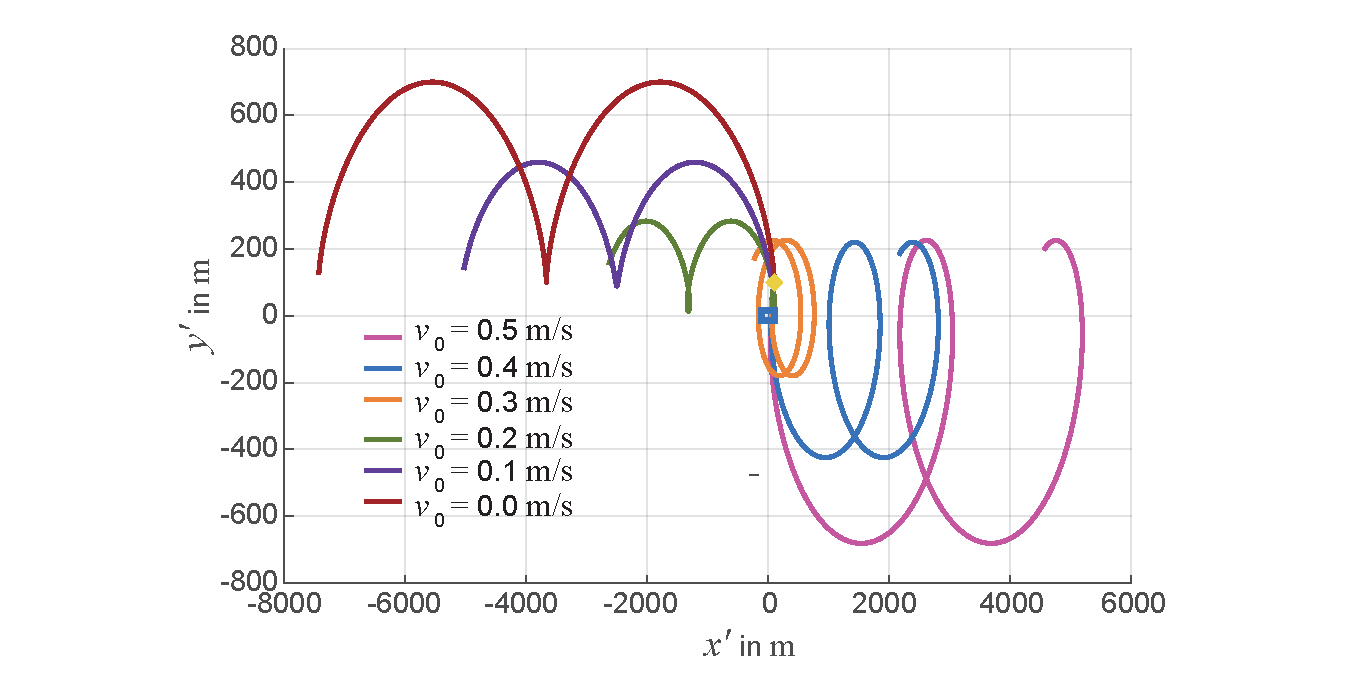
\includegraphics[width=\textwidth]{RendezvousAstronaut01.pdf} 
	%\caption[Astronaut au�erhalb der ISS.]{Astronaut au�erhalb der ISS. Der Astronaut befindet sich initial bei $x_0'=y_0'=\SI{100}{\metre}$ und bewegt sich mit einer Anfangsgeschwindigkeit $v_0$ (also keine initiale Relativgeschwindigkeit zum Ziel, d.h. $\dot{x}_0'=\dot{y}_0=0'$) genau in Richtung auf die Station zu. Selbst bei $v_0=0$ entfernt sich der Astronaut mit der Zeit von der Raumstation. Dargestellt sind die L�sungen der Clohessy-Wiltshire-Gleichungen wie im \mscr~ \mladynref{Rendezvous01.m} im Detail ausgef�hrt.}
	%\label{abb:adyn_rendezvous02}
%\end{figure}
%
  %\item[b)]
    %Was passiert, wenn der Astronaut seinen R�ckkehrantrieb (englisch \textit{Return-Thruster}) mit einem Antriebsverm�gen von $\SI{1}{\metre\per\second}$ einsetzt?   
		%Intuitiv \anf{zielt} der Astronaut mit seinem auf dem R�cksto�-Prinzip basierenden Thruster genau in Richtung ISS, also mit
    %\begin{align*}
        %\vec{v}_0 = 
        %\begin{pmatrix}
            %\dot{x}_0'\\
            %\dot{y}_0'\\
            %\dot{z}_0'
        %\end{pmatrix}
        %= \frac{1}{\sqrt{2}}
        %\begin{pmatrix}
            %1\\
            %1\\
            %0
        %\end{pmatrix}
        %\SI{}{\metre\per\second}\,.
    %\end{align*}
    %Leider wird durch die kombinierte Wirkung der Gezeiten und Coriolis-Kraft der Astronaut die ISS verfehlen, wie Gleichung \eqref{eq:adyn_rendez23} und \figref{adyn_rendezvous02} und \figref{adyn_rendezvous03}a zeigen.\\
    %\item[c)]
    %Wie muss der Astronaut beim Abfeuern seines Thrusters zielen, damit er die ISS sicher erreicht? \\
		%$\dot{x}_0'$, $\dot{y}_0'$ ergeben sich aus \eqref{eq:adyn_rendez24}. Wir k�nnen noch eine kleine Eigengeschwindigkeit des Astronauten vor dem Starten des Thrusters mit $\vec{v}_\text{vor} = \lk\dot{x}_{\text{vor},0'}, \dot{y}_{\text{vor},0'}\rk$ annehmen und erhalten den richtigen Zielwinkel:
    %\begin{align}
        %\tan\lk\gamma\rk = \frac{\Delta v_y}{\Delta v_x} = \frac{\dot{y}_0' -\dot{y}_{\text{vor},0'}}{\dot{x}_0'- \dot{x}_{\text{vor},0'}} \,. \label{eq:adyn_rendez27}
    %\end{align}
%\end{enumerate}
%In der Realit�t wird sich der Astronaut nat�rlich in kleinen Minisch�ben iterativ der ISS n�hern, doch auch daf�r gelten die abgeleiteten Formeln.
%
%\begin{figure}[H]
	%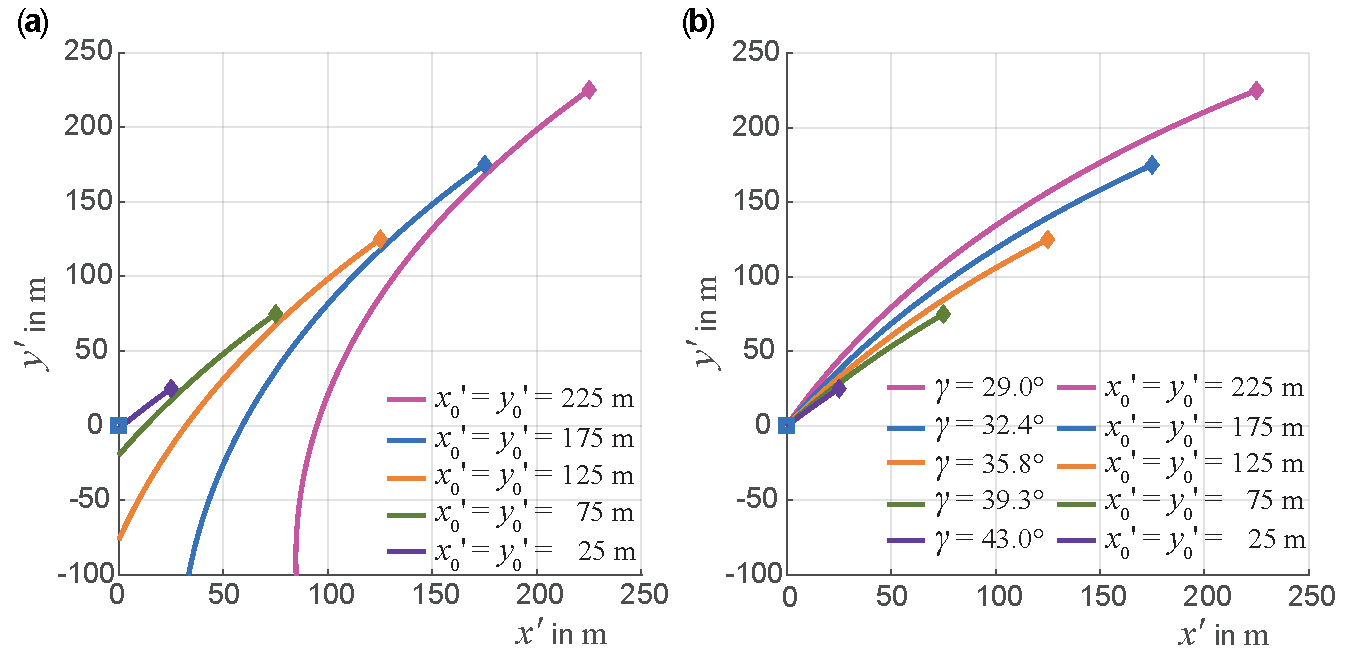
\includegraphics[width=\textwidth]{RendezvousAstronaut02.pdf} 
	%\caption[Astronaut au�erhalb der ISS.]{Astronaut au�erhalb der ISS. \fa Der Astronaut befindet sich initial bei $x_0'=y_0'=\SI{25}{\metre} \ldots \SI{225}{\metre}$ und "`zielt"' mit seinem Antriebssystem  mit einer Anfangsgeschwindigkeit $v_0$ genau in Richtung auf die Station. L�sung der Hill-Gleichungen. \fb Der Astronaut befindet sich ebenfalls initial bei $x_0'=y_0'=\SI{25}{\metre} \ldots \SI{225}{\metre}$ und bewegt sich mit einem optimierten Zielwinkel $\gamma$ der Richtung Anfangsgeschwindigkeit von $v_0 = \SI{1}{\metre\per\second}$ auf die Station zu (L�sung der Clohessy-Wiltshire-Gleichungen\index{Clohessy-Wiltshire-Gleichungen}). Offensichtlich wird der Astronaut erst bei Entfernung von kleiner als 50 m bei direkter Anzielung der Station auch bei dieser wirklich ankommen. Die Rechnungen sind im \mscr~ \mladynref{Rendezvous02.m} im Detail ausgef�hrt.}
	%\label{abb:adyn_rendezvous03}
%\end{figure}
%
%\label{bsp:adyn_stranded_astronaut}
%\end{example}
%
%

Wir verweisen auf die MATLAB-Skripte \mladynref{Rendezvous04.m} und \mladynref{Rendezvous05.m}.

\begin{figure}[H]
	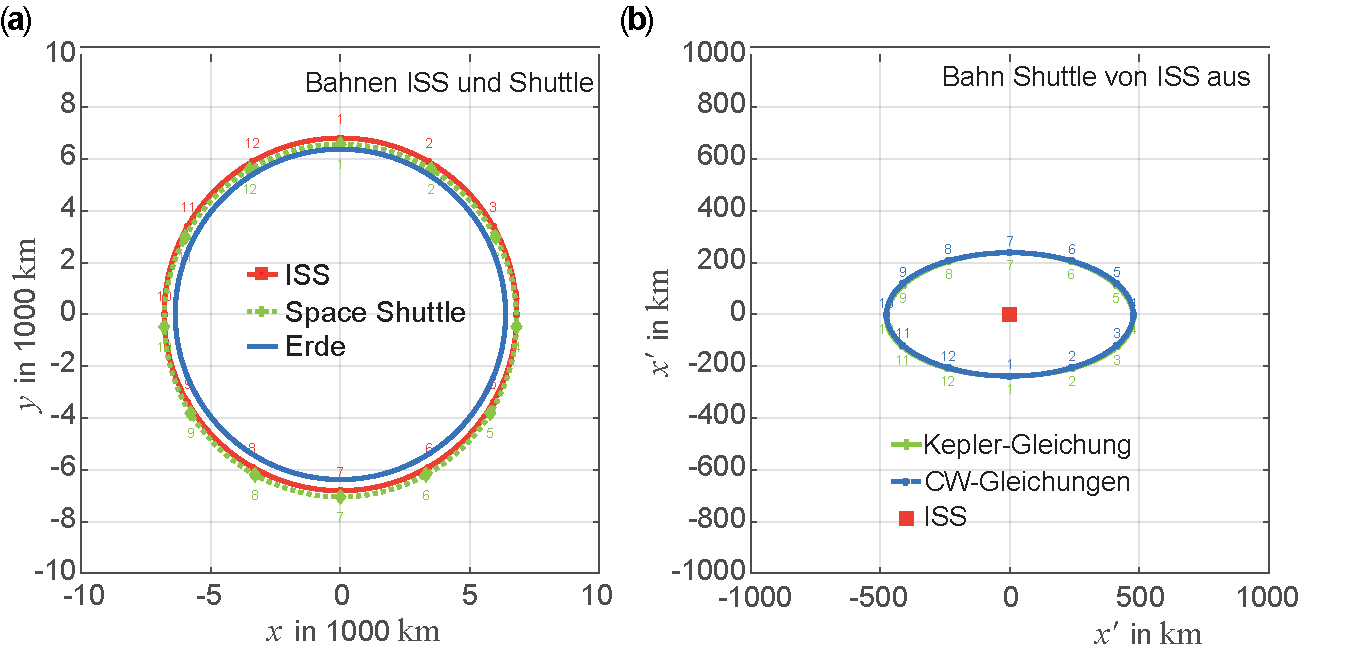
\includegraphics[width=\textwidth]{SpaceShuttle2ISS.pdf} 
	\caption[Space Shuttle und ISS in unterschiedlichen Umlaufbahnen.]{Space Shuttle und ISS in unterschiedlichen Umlaufbahnen. \fa Bahnen von ISS und Space Shuttle. Die Shuttle Bahn ist fiktiv, um das Prinzip zu erl�utern. In der Realit�t war die Shuttle Bahn viel n�her an der ISS. \fb Bahn Space Shuttle von ISS aus. L�sungen nach der Kepler-Gleichung mit Drehung des mitbewegten \KOS des Ziels und CW-L�sung im Vergleich. Die �bereinstimmung der exakten L�sungen nach der Kepler-Gleichung mit der CW-L�sung ist sehr gut, da auf Grund der Parameter die Linearisierungsbedingung f�r die CW-Gleichung relativ gut erf�llt ist.}
	\label{abb:adyn_rendezvous04Lsg}
\end{figure}

\end{sol} 
\textcolor{blue} {$\rightarrow$ zur} \probref{adyn_rendezvous01}.\\
\noindent\rule[1ex]{\textwidth}{0.5pt}  \newpage  \clearpage


%-----------------------------------------------------------------------------------------------------------

\begin{sol}{prob:adyn_rendezvous02}\label{lsg:adyn_rendezvous02} %�bung23
\textbf{Rendezvous Apollo 11 CSM und LM}\\

Die L�sung zum Rendezvous von LM und CSM von Apollo 11 in der Mondumlaufbahn ist im Detail im \mscr~\mladynref{LMCSMApollo11.m} als Berechnung der Kinematik des Rendezvous �ber die Clohessy-Wiltshire-Gleichungen ausgef�hrt. Wir erhalten die \figref{adyn_rendezvous06} aus \kap{adyn_rendezvous_apollo11}.\\

\begin{figure}[H]
	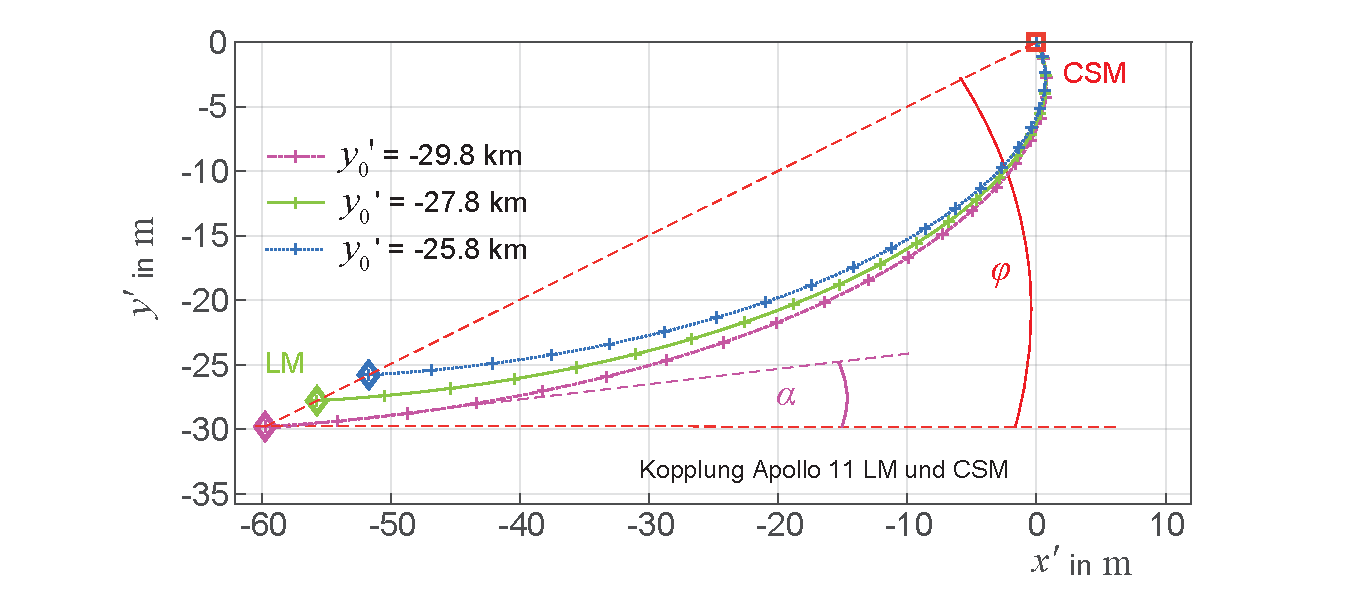
\includegraphics[width=\textwidth]{Apollo11LMCSMTrajektorie.pdf} 
	\caption[Trajektorien des LM im Anflug auf das CSM von Apollo 11.]{Trajektorien des LM im Anflug auf das CSM von Apollo 11 f�r verschiedene H�hen des TPI-Burn. Siehe \probref{adyn_rendezvous02} \bzw \mscr{}\mladynref{LMCSMApollo11.m}.}
	\label{abb:adyn_rendezvous06_uebung}
\end{figure}

\end{sol} 
\textcolor{blue} {$\rightarrow$ zur} \probref{adyn_rendezvous02}.\\
\noindent\rule[1ex]{\textwidth}{0.5pt} \newpage \clearpage 

%-----------------------------------------------------------------------------------------------------------

\begin{sol}{prob:adyn_rendezvous03}\label{lsg:adyn_rendezvous03} %�bung24
\textbf{Planung einer Apollo Mission - \textit{Free Return Trajectory}}\\

\begin{subprobs}
\subprob{Absch�tzungen}
Wir wollen als erstes eine Absch�tzung f�r die Flugzeit zum Mond treffen und nehmen dabei eine koplanare Bewegung von Flugbahn und Mondbahn an, letztere wird auch noch als Kreisbahn angenommen (\figref{adyn_FRT01}).\\
Der Punkt $\mathrm{P}_0$ (Abstand $r_0$ vom Erdzentrum) in der Parkbahn um die Erde, aus der der Einschuss (Injektion) in die translunare Bahn erfolgt, wird \textit{(Translunar Injection Point} (TLI) genannt. Dort gilt f�r die Energie und den Drehimpuls des Raumschiffs bezogen auf das Erd-\KOS:
\begin{align}
H_0 = \frac{v_0{}^2}{2} - \frac{\mu_\text{E}}{r_0}\,, & L_0 = r_0\,v_0\,\cos\gamma_0\,. \label{eq:adyn_lsg_FRT01}
\end{align}
Hierin sind $v_0\,\cos\gamma_0$ die Komponente der Raumschiff-Geschwindigkeit in Richtung lokaler Horizont mit $\gamma_0$ als der FPA bei $r_0$.\\
Damit ergeben sich f�r die Ellipse zum Mond folgende Ellipsenparameter (vergleiche auch Gleichungen \eqref{eq:hm_bewgl1} und \eqref{eq:hm_relations1}):
\begin{align}
\begin{split}
    p &= \frac{L_0{}^2}{\mu_ \text{E}}\,,~~~~ a = -\frac{\mu_\text{E}}{2H_0}\,, ~~~~
    e = \sqrt{1 - \frac{p}{a}} \,=\, \sqrt{1+\frac{L_0{}^2}{\mu_\text{E}{}^2}\,2H_0}\,~.
\end{split} \label{eq:adyn_lsg_FRT02}
\end{align}
\begin{figure}[H]
	\includegraphics[width=\textwidth]{Transfer2Moon.pdf} 
	\caption[Geometrie des Flugs zum Mond.]{Vereinfachte Geometrie des Flugs eines Raumschiffes zum Mond. Im Bild wurde eine koplanare Bewegung von Raumschiff und Mond in der Ekliptik angenommen (Draufsicht auf die Ekliptik). (Nach \cite{Bate1971}).}
	\label{abb:adyn_FRT01}
\end{figure}

In \figref{adyn_FRT01} definieren wir aus der Geometrie f�r die weitere mathematische Behandlung folgende Parameter:
\begin{align*} 
    r_0 && &\text{geozentrischer Abstand des Raumschiffs bei Injektion in die translunare Bahn} \\
    r_1 && &\text{geozentrischer Abstand des Raumschiffs beim Erreichen der SOI des Mondes}\\
    && &r_1 = \sqrt{r_{\text{EM}}{}^2 + R_{\text{SOI, M}}{}^2 - 2 r_{\text{EM}} R_{\text{SOI, M}} \cos\gamma_1} \\
    r_\text{EM} && &\text{Abstand der Massezentren von Erde und Mond}      \\
    R_\text{SOI,M} && &\text{Radius der SOI des Mondes}\\
    \varphi_0 && &\text{geozentrischer Phasenwinkel des Mondes bei Abflug (TLI) relativ zur}\\
    && &\text{Verbindungslinie Erde/Raumschiff}\\
    \varphi_1 && &\text{geozentrischer Phasenwinkel des Mondes bei Ankunft des Raumschiffs }\\
    && &\text{an der SOI relativ zur Verbindungslinie Erde/Raumschiff}\\
    \lambda_1 && &\text{selenozentrischer Winkel zwischen Ankunftsort des Raumschiffs}\\
    && &\text{an der SOI des Mondes und der Verbindungslinie Erde/Mond}\\
    \gamma_0,\gamma_1 && &\text{FPA des Raumschiffs bei TLI \bzw Ankunft an der SOI des Mondes}\\
    \upsilon_0,\upsilon_1 && &\text{wahre Anomalien der Ellipsenbahn bei TLI \bzw Ankunft SOI des Mondes}\\
    \omega_\text{M} && &\text{Umlaufgeschwindigkeit des Mondes}\,\approx \SI{2.649e-6}{\radian\per\second}\\
		a, e, P && &\text{Parameter der Transferellipse zum Mond}
\end{align*}
F�r eine Planung eines Fluges zum Mond startet man mit Vorgaben f�r $r_0,\,v_0,\,\gamma_0$ und $\lambda_1$ und berechnet die Flugzeit $t_\text{F} = \mathrm{ToF}$,\;$\varphi_0$,\, $\varphi_1$ und $\gamma_1$. Ergeben sich daraus keine sinnvollen Werte, so muss man $r_0,\,v_0,\,\gamma_0$ und $\lambda_1$ variieren. \\
Aus den Ellipsenparametern $a$, $p$, $e$ lassen sich nun bei bekannten $r_0,r_1$ die jeweiligen wahren Anomalien berechnen.
\begin{align}
\begin{split}
    \cos\upsilon_0 &= \frac{p - r_0}{\e\,r_0} \,,\\
    \cos \upsilon_1 &= \frac{p - r_1}{\e \,r_1} \quad \text{mit} \quad r_1 = \sqrt{r_{\text{EM}}{}^2 + R_{\text{SOI,M}}{}^2 - 2 r_{\text{EM}}\,R_{\text{SOI,M}} \cos \lambda_1}
\end{split}\label{eq:adyn_lsg_FRT03}
\end{align}
Die Flugzeit zum Mond ergibt sich �ber die Kepler-Gleichung zu:
\begin{align}
    t_\text{F} = t_1 - t_0 = \lk\sqrt{\frac{a^3}{\mu_\text{E}}}\rk \lek E_1 - E_0 - \e\,\lk \sin E_1 - \sin E_0\rk\rek\label{eq:adyn_lsg_FRT04}
\end{align}
wobei sich die exzentrische Anomalien $E_i~~(i=1,2)$ entweder aus
\begin{align}
\begin{split}
    \cos E_i &= \frac{\e - \cos \upsilon_i}{1 + \e \cos \upsilon_i} = \lk 1 - \frac{r_i}{a}\rk\,\frac{1}{\e}\\
    \text{oder}\quad \tan \frac{E_i}{2} &= \sqrt{\frac{1-\e}{1+\e}}\,\tan \lk \frac{\upsilon_i}{2} \rk    
\end{split}\label{eq:adyn_lsg_FRT05}
\end{align}
ergeben (\vgl Gleichungen \eqref{eq:hm_r_param_ellipse} und \eqref{eq:hm_nu(t)_alternativ}).\\
Wir brauchen noch den Winkel $\varphi_1$, dieser ergibt sich nach dem Sinussatz aus
\begin{align}
    \sin\varphi_1 = \frac{R_{\text{SOI,M}}}{r_1}\,\sin\lambda_1 \,. \label{eq:adyn_lsg_FRT06}
\end{align}
F�r eine Absch�tzung der Flugzeiten wollen wir annehmen, dass $\gamma_0 \approx 0$ ist. Wir k�nnen dann die Flugzeiten f�r verschiedene $\lambda_1$ \bzw $\varphi_1$ als Funktion der TLI-Geschwindigkeit $v_0$ berechnen.

\begin{figure}[H]
	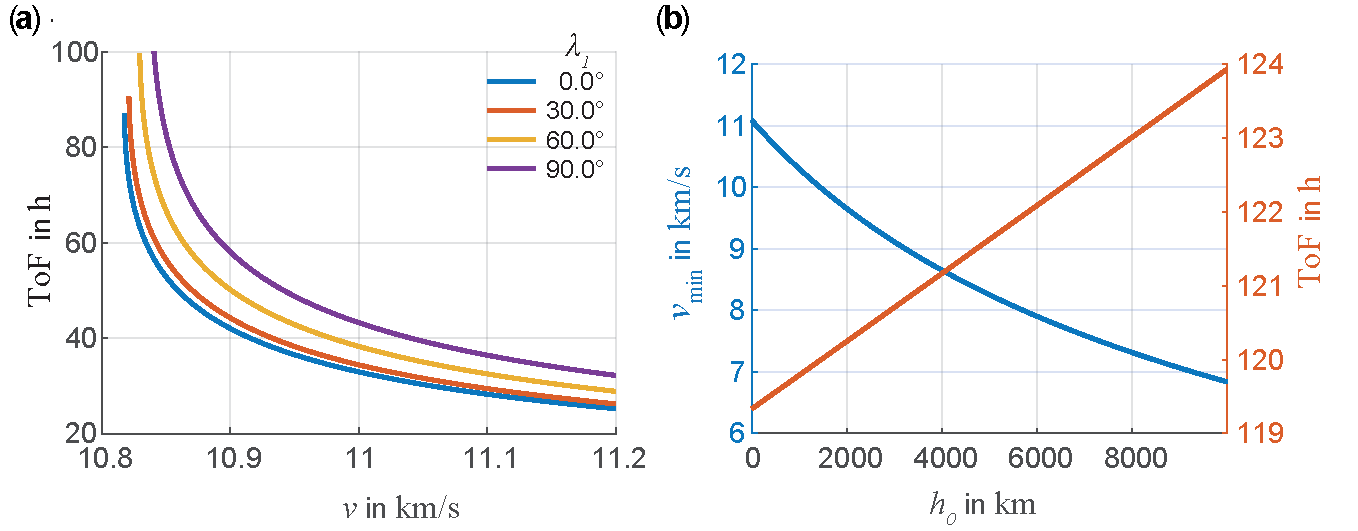
\includegraphics[width=\textwidth]{Transfer2MoonTOF.pdf} 
	\caption[Flugzeiten und Minimalgeschwindigkeit zum Mond.]{Flugzeiten und Minimalgeschwindigkeit zum Mond. \fa ToF als Funktion der TLI-Geschwindigkeit $v_0$ \fb Minimum-Geschwindigkeit $v_\text{min}$ f�r TLI und zugeh�rige ToF als Funktion des Radius $r_0$ der erdnahen Kreisbahn. Siehe \mscr~\mladynref{Transfer2Moon.m}.}
	\label{abb:adyn_FRT02}
\end{figure}

Man erkennt aus \figref{adyn_FRT02}a, dass es eine minimale Geschwindigkeit $v_{\text{min}}$ (abh�ngig vom Winkel $\lambda_1$) gibt, um �berhaupt in endlicher Zeit den Mond zu erreichen. Diese liegt bei etwas �ber $\SI{10.8}{\km\per\second}$ f�r $\lambda_1 =0$ und ist ebenfalls abh�ngig und der H�he $h_0$ der Parkbahn in Erdn�he.\\
Man kann nun eine einfache numerische Absch�tzung f�r $v_{\text{min}}$ machen, wenn man annimmt, dass die TLI am Perig�um erfolgen soll.
Dann ist definitiv $\gamma_0 = 0$ und das Apog�um der elliptischen translunaren Bahn entspricht dann $r_{\text{EM}}$ (\bzw $r_{\text{EM}} - R_{\text{SOI,M}}$, wenn wir die SOI ber�cksichtigen wollen). Wir finden also:
\begin{align}
     2a_0 &= r_0 + r_{\text{EM}} ~~~\text{und}~~~H_0 = -\frac{\mu_\text{E}}{2a} = \frac{v_{\text{min}}{}^2}{2} - \frac{\mu_\text{E}}{r_0} \nonumber \\
    \rightarrow \quad v_{\text{min}}{}^2 &= \frac{2\mu_\text{E}}{r_0}\,\lk 1 - \frac{1}{1 + r_{\text{EM}}/r_0}\rk ~~ \text{und} ~~~ \text{ToF}_{\text{max}} = \pi \sqrt{\frac{a_0{}^3}{\mu_\text{E}}} \,. \label{eq:adyn_lsg_FRT07}
\end{align}
Man erh�lt dann \zb f�r $h_0 = \SI{400}{\km}$ eine minimale notwendige Geschwindigkeit von $v_{\text{min}} = \SI{10.75}{\km\per\second}$ und eine (maximale) Flugzeit von $ \text{ToF}_{\text{max}} = \SI{119.5}{\hour}$ (\figref{adyn_FRT03}), 
was wesentlich l�nger ist, als \zb Apollo 11 zum Mond brauchte.\\
Man erkennt sehr sch�n aus \figref{adyn_FRT02}, wie kleine �nderungen der TLI-Anfangsgeschwindigkeit die Flugzeit wesentlich verk�rzen.

\subprob {\textit{Patch Conic} - N�herung}

Nach diesen grunds�tzlichen �berlegungen wollen wir nun die Bahn genauer berechnen und dabei das Konzept der SOI (siehe \kap{adyn_gravity_assist} \bzw \probref{adyn_SOI}) benutzen. Bisher haben wir ja die Gravitationswirkung des Mondes vernachl�ssigt. Wir arbeiten in den relevanten Bereichen jeweils nur mit der SOI der Erde \bzw des Mondes. Dies f�hrt auf das sogenannte Konzept der \textit{Patched Conic} (der "`aneinandergest�ckelten Kegelschnitte"', \vgl auch \probref{adyn_SOI}). 

\begin{figure}[H]
	\includegraphics[width=\textwidth]{Transfer2MoonPP.pdf} 
	\caption[Geometrie des Transfers zum Mond am \textit{Patch Point}.]{Geometrie des Transfers zum Mond am \textit{Patch Point}. Die Koordinaten im selenozentrischen \KOS werden mit dem Index 2 bezeichnet und sind in rot gezeichnet. Der Winkel $\varepsilon_2$ bezeichnet den anf�nglichen selenozentrischen Winkel der Geschwindigkeit des Raumschiffs relativ zum Mondzentrum. (Nach \cite{Bate1971}.)}
	\label{abb:adyn_FRT03}
\end{figure}

Wir berechnen zun�chst die Transferphase vom TLI bis zum Erreichen der SOI des Mondes. Dazu berechnen wir �ber \eqref{eq:adyn_lsg_FRT03}-\eqref{eq:adyn_lsg_FRT05} die ToF und auch den geozentrischen Phasenwinkel $\varphi_0$, den der Mond bei der TLI haben muss:
\begin{align}
    \varphi_0 = \upsilon_1 - \upsilon_0 - \gamma_1 - \omega_{\text{M}}\,  \lk t_1 - t_0\rk\,. \label{eq:adyn_lsg_FRT08}
\end{align}
Wir schauen uns nun genauer die Bedingungen am sogenannten \textit{Patch Point}, dem Punkt PP an. Wir bestimmen dort zun�chst die Geschwindigkeit $\vec{v}_2$ des Raumschiffs im selenozentrischen (\dh lunaren) \KOS:
\begin{align}
\begin{split}
    \vec{v}_2 &= -\vec{v}_{\text{M}} + \vec{v}_1\\
    v_2 &= \sqrt{v_1{}^2 + v_{\text{M}}{}^2 - 2 v_1\,v_{\text{M}}\,\cos \lk \gamma_1 - \varphi_1\rk} 
\end{split}\label{eq:adyn_lsg_FRT09}
\end{align}
mit
\begin{align*}
    v_{\text{M}} = \omega_{\text{M}}\,r_{\text{EM}} \approx \SI{1.018}{\km\per\second}.
\end{align*}
Ferner gilt am Punkt PP $r_2 = R_{\text{SOI,M}}$ und 
\begin{align}
    \varepsilon_2 = \arcsin \lk\frac{v_\text{M}}{v_2}\,\cos\lambda_1 - \frac{v_1}{v_2}\,\cos\lk \lambda_1 + \varphi_1-\gamma_1\rk\rk \,. \label{eq:adyn_lsg_FRT10}
\end{align}
Letztere Beziehung kann man sich ebenfalls aus \figref{adyn_FRT03} �ber
\begin{align*}
    v_2\,\sin\epsilon_2 = v_{\text{M}}\,\cos \lambda_1 - v_1\,\cos\lk\lambda_1 + \varphi_1 - \gamma_1\rk
\end{align*}
herleiten. F�r eine direkte Landung auf dem Mond muss der Winkel $\varepsilon_2$ logischerweise $0$ sein. 
F�r alle anderen F�lle kann man nun mit den \anf{lunaren} Anfangsbedingungen $r_2$, $v_2$ und $\epsilon_2$ drei m�gliche Trajektorien um den Mond herum unterscheiden:
\begin{enumerate}
    \item [1)] Aufschlag auf den Mond: In diesem Fall ist das Periselenium $r_{\text{P,M}}$ (kleinster Abstand der Bahn vom Mondzentrum) kleiner als der Mondradius $R_{\text{M}}$.
    \item [2)] Mondumlaufbahn, \dh Einschwenken auf eine Mondumlaufbahn durch Abbremsen/Beschleunigen auf die notwendige Umlaufgeschwindigkeit  $v_3$.
    \item [3)] Mondumrundung (\zb als \textit{Free Return Trajektory} (FRT)), wobei besonders das Periselenium und die Bedingungen ($r_3$, $v_3$, $\gamma_3$, $\lambda_3$) beim Verlassen der SOI des Mondes interessant sind, da diese in ma�gebliche die R�ckkehrbahn zur Erde bestimmen.
\end{enumerate}
Wir m�ssen daher als n�chstes das Periselenium $r_\text{P,M}$ berechnen, da wir das ja in jedem der drei F�lle zur Bewertung der Bahn um den Mond brauchen. In der SOI des Mondes gilt im \KOS des Mondes gilt nat�rlich wieder Energie- und Drehimpulserhaltung:
\begin{align}
\begin{split}
    H_2 &= \frac{v_2{}^2}{2} - \frac{\mu_\text{M}}{r_2}\,~~\text{mit}~~ \mu_ \text{M} = G\,M_\text{M} \,\\
		L_2 &=  r_2 \, v_2\,\cos \gamma_2 = r_2\,v_2\,\sin \varepsilon_2 \,, ~~\text{da}~~ \gamma_2 = 90^\degree - \varepsilon_2\,.
\end{split}\label{eq:adyn_lsg_FRT11}
\end{align}
Wie bei der Berechnung der Transferellipse finden wir die Kegelschnittparameter\footnote{Der Kegelschnitt wird \ia eine Hyperbel sein.} f�r die Mondbahn:
\begin{align}
    p_2 = \frac{L^2}{\mu_\text{M}}\,, \quad e_2 = \sqrt{1 + \frac{2 H_2\,L^2}{\mu_\text{M}{}^2}} \label{eq:adyn_lsg_FRT12}
\end{align}
und daraus
\begin{align}
    r_\text{P,M} = \frac{p_2}{1 + \e}\,, \quad v_\text{P,M} = \sqrt{2 \lk H_2 + \frac{\mu_\text{M}}{r_\text{P,M}} \rk} \label{eq:adyn_lsg_FRT13}
\end{align}
Wir wollen als Beispiel durchrechnen:
\begin{align*}
    r_0 &= \SI{300}{\km} + R_\text{E} = \SI{6678}{\km}\,,~~
    v_0 = \SI{10.87}{\km\per\second}\,,~~
    \gamma_0 = 0^\degree\,,~~
    \lambda_1 = 30^\degree\,.
\end{align*}
Ohne weitere Kurskorrekturen wird die geringste Entfernung zur Mondoberfl�che
\begin{align*}
    h_\text{P,M} = r_\text{P,M} - R_\text{M} = r_\text{P,M} - \SI{1737.4}{\km} = \SI{1413.6}{\km}\,.
\end{align*}
Wie bereits erw�hnt, kommt es f�r  $h_\text{P,M} < 0$ zur Landung \bzw zum Aufschlag auf dem Mond, abh�ngig von $v\lk h_\text{M} = 0\rk$ und je nach Verf�gbarkeit von Bremsm�glichkeiten.\\

\begin{figure}[H]
	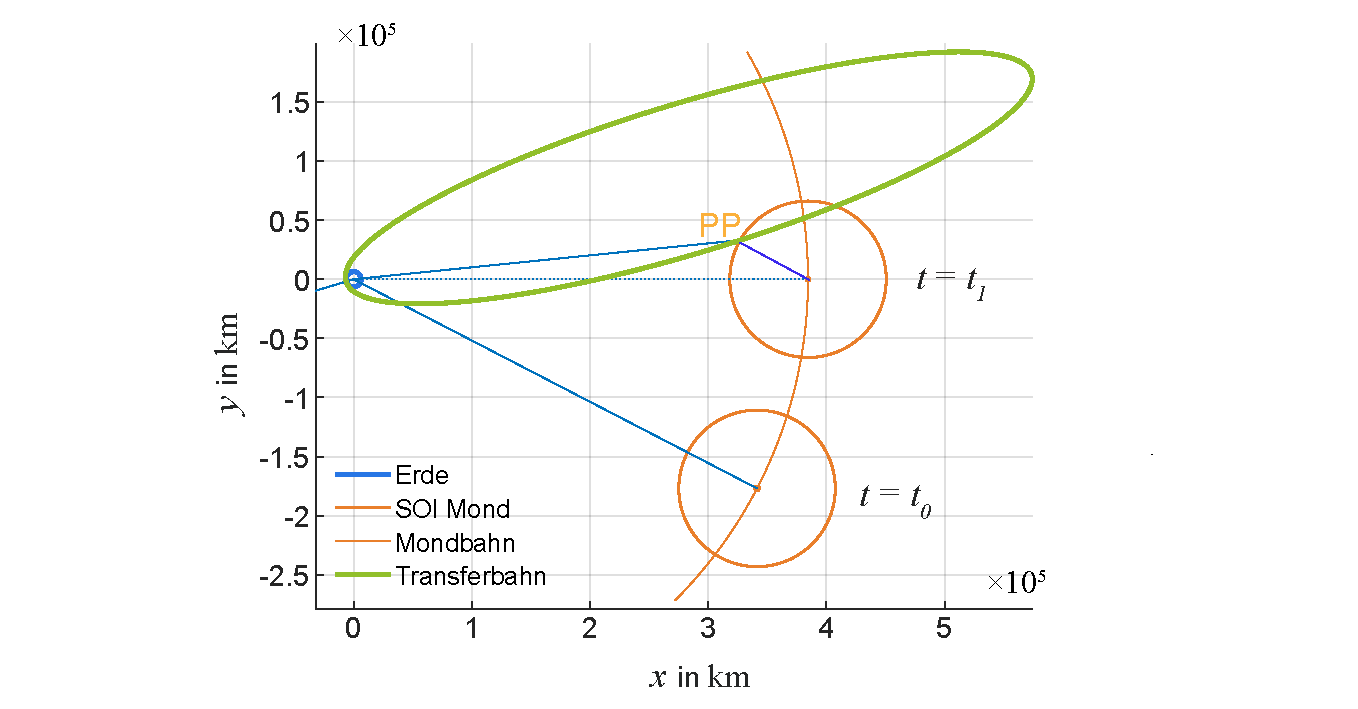
\includegraphics[width=\textwidth]{Transfer2Moon04.pdf} 
	\caption[Berechnete Geometrie des Transfers zum Mond.]{Berechnete Geometrie des Transfers eines Raumschiffes zum Mond. In der Rechnung wurde eine koplanare Bewegung von Raumschiff und Mond in der Ekliptik angenommen. Parameter siehe Tabelle \ref{tab:adyn_FRT01} und \mscr~\mladynref{Transfer2MoonExample.m}.}
	\label{abb:adyn_FRT04}
\end{figure}


Die Parameter f�r die \figref{adyn_FRT04} und \figref{adyn_FRT05} sind in folgender Tabelle gelistet:
\begin{table}[h!]
\centering
\begin{tabular}{|c|c|c|c|c|c|}
\hline
\multicolumn{6}{|l|}{\textbf{Vorgaben und Abflugparameter @TLI}} \\
\hline
$h_0$ (km) & $\gamma_0$ ($\degree$) & $v_0$ (km/s) & $\lambda_1$ ($\degree$) & &   \\
\hline
300.0 & 0.0 & 10.87 & 30.0 & &  \\
\hline
\multicolumn{6}{|l|}{\textbf{Abflugparameter @TLI}} \\
\hline
$a_0$ (km) & $p_0$ (km) & $\e_0$  & $\phi_0$ ($\degree$) &  &  \\
\hline
$\SI{3.03e5}{}$& $\SI{1.32e4}{}$& 0.9780 & 135.77 & &   \\
\hline
\multicolumn{6}{|l|}{\textbf{Parameter auf Transfer zum Mond}} \\
\hline
$v_1$ (km/s) & $v_2$ (km/s) & $\upsilon_1$ &$\upsilon_2$ & $\mathrm{TOF}$ (h) &  \\
\hline
1.054 & 1.220 &0.0 & 5.78 & 50.15&  \\
\hline
\multicolumn{6}{|l|}{\textbf{Parameter am Mond}} \\
\hline
$r_2$ (km) & $\epsilon_2$ ($\degree$) & $p_2$ (km) &$\e_2$ & $h_\text{PM}$ (km)& $\mathrm{TOF}_\text{SOI}$ (h)  \\
\hline
$\SI{6.62e4}{}$ & 4.72 & 9014.8 & 1.8610 & 1413.6 & 28.05 \\
\hline
\end{tabular}
\caption{Parameter f�r \textit{Patch Conic} N�herung} \label{tab:adyn_FRT01}
\end{table}
Hierin ist $\mathrm{TOF}$ die Flugzeit von der TLI bis zum Erreichen der SOI des Mondes und $\mathrm{TOF}_\text{SOI}$ die Flugzeit zum Durchfliegen der SOI des Mondes. \\
Insgesamt ergibt sich f�r einen Flug bis zur R�ckseite des Mondes eine Gesamtflugzeit von
\begin{align*}
    t_\text{F} = \mathrm{TOF} + \frac{1}{2} \mathrm{TOF}_\text{SOI} = \SI{50.15}{\hour} + \SI{14.025}{\hour} \approx \SI{64.175}{\hour}\,,
\end{align*}
also etwa weniger als 3 Tage und damit auch etwas schneller als Apollo 8 unterwegs war.\\

\begin{figure}[H]
	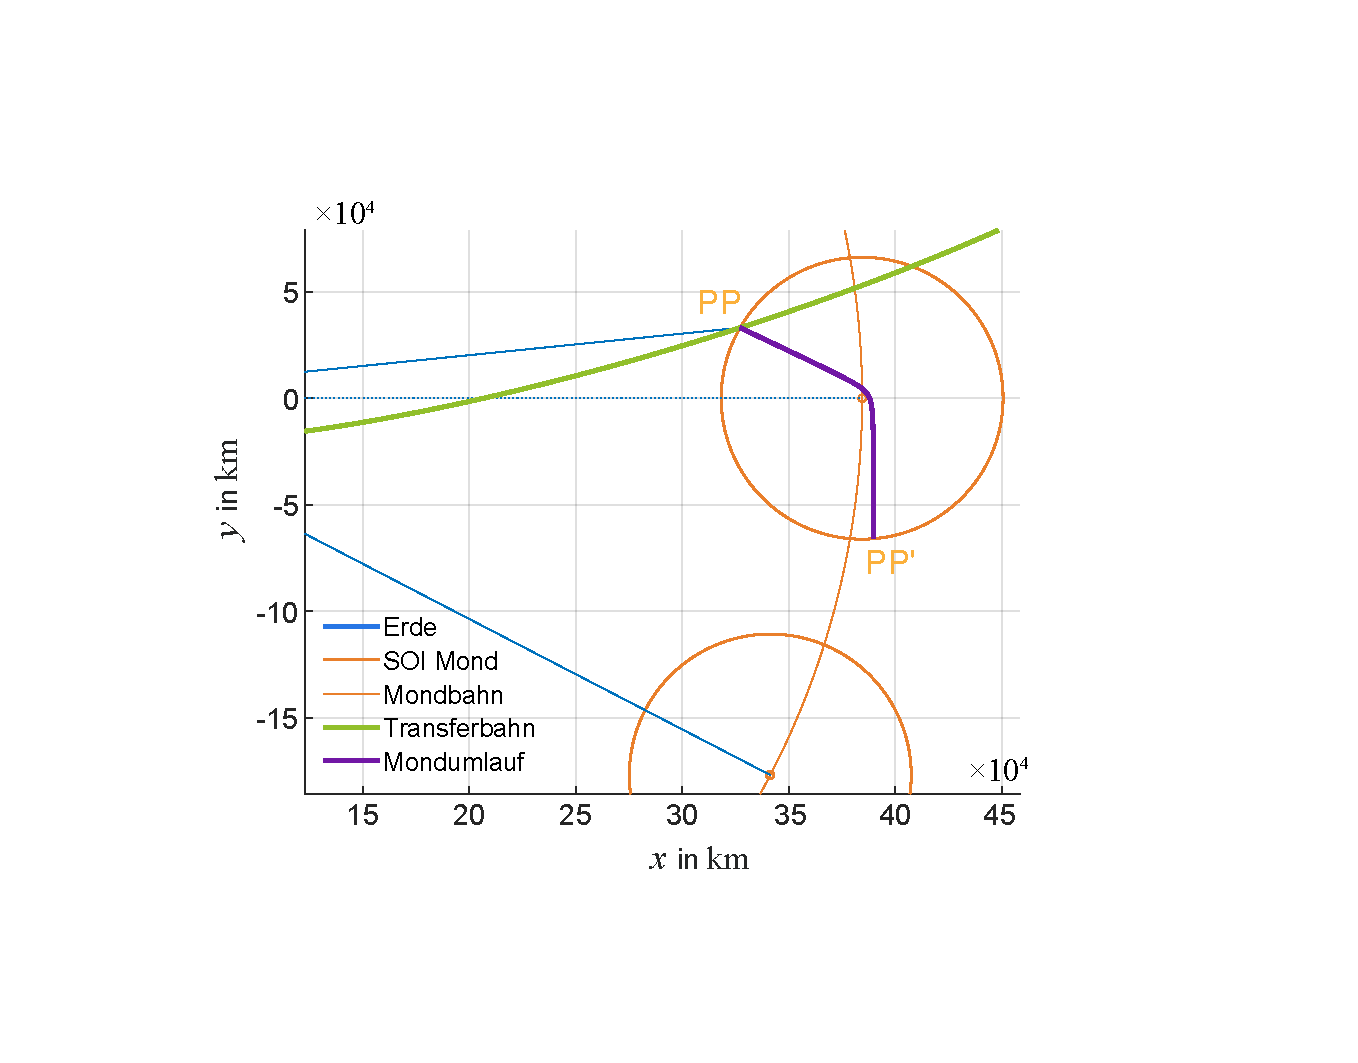
\includegraphics[width=\textwidth]{Transfer2Moon05.pdf} 
	\caption[Berechnete Geometrie des Transfers zum Mond am \textit{Patch Point}.]{Berechnete Geometrie des Transfers zum Mond am \textit{Patch Point}, sowie Mondumlauf. Die lila Kurve zeigt die Bahn des Raumschiffs im \KOS des Mondes. In der Rechnung wurde eine koplanare Bewegung von Raumschiff und Mond in der Ekliptik angenommen. Parameter siehe Tabelle Parameter siehe Tabelle \ref{tab:adyn_FRT01} und \mscr~\mladynref{Transfer2MoonExample.m}. Man beachte, dass \figref{adyn_FRT05} die Bewegung im \KOS des Mondes zeigt und nicht im als Inertialsystem angenommenen geozentrischen \KOS der Erde. F�r eine Energie $H_2 > 0$ wird $\e_2 > 1$ und damit die Bewegung um den Mond eine Hyperbel. Man �berlege sich Analogien zur Behandlung des Gravity-Assist-Man�vers in \kap{adyn_gravity_assist}.}
	\label{abb:adyn_FRT05}
\end{figure}

Man kann die Werte am Punkt PP' berechnen und dann weiter transformieren in das Erd-\KOS, um zu sehen, ob eine \textit{Free Return Trajectory} vorliegt, ganz analog wie beim Swing-By-Man�ver.\\
Wir wollen jedoch im Folgenden die Rechnungen komplett, also auch die Bewegung um den Mond herum im Inertialsystem numerisch machen und k�nnen dabei als Startwert die Parameter der \textit{Patch Conic}-Rechnung �bernehmen.

\newpage
\subprob{Numerische Rechnung Vergleich \textit{Patch Conic} und 1. N�herung}

Wir wollen nun konkret den Raumflug von Apollo 13 anschauen und w�hlen  entsprechend des NASA Flight Journal (\url{https://www.nasa.gov/history/afj/ap13fj/index.html}) $h_0=\SI{169.609}{\km}$. Ebenso benutzen die Ergebnisse der \textit{Patch Conic} N�herung (\figref{adyn_FRT06}) als Startwerte f�r die numerische Rechnung und betrachten zun�chst die Erde als ruhend und den Mond auf einer Kreisbahn umlaufend. 

\begin{figure}[H]
	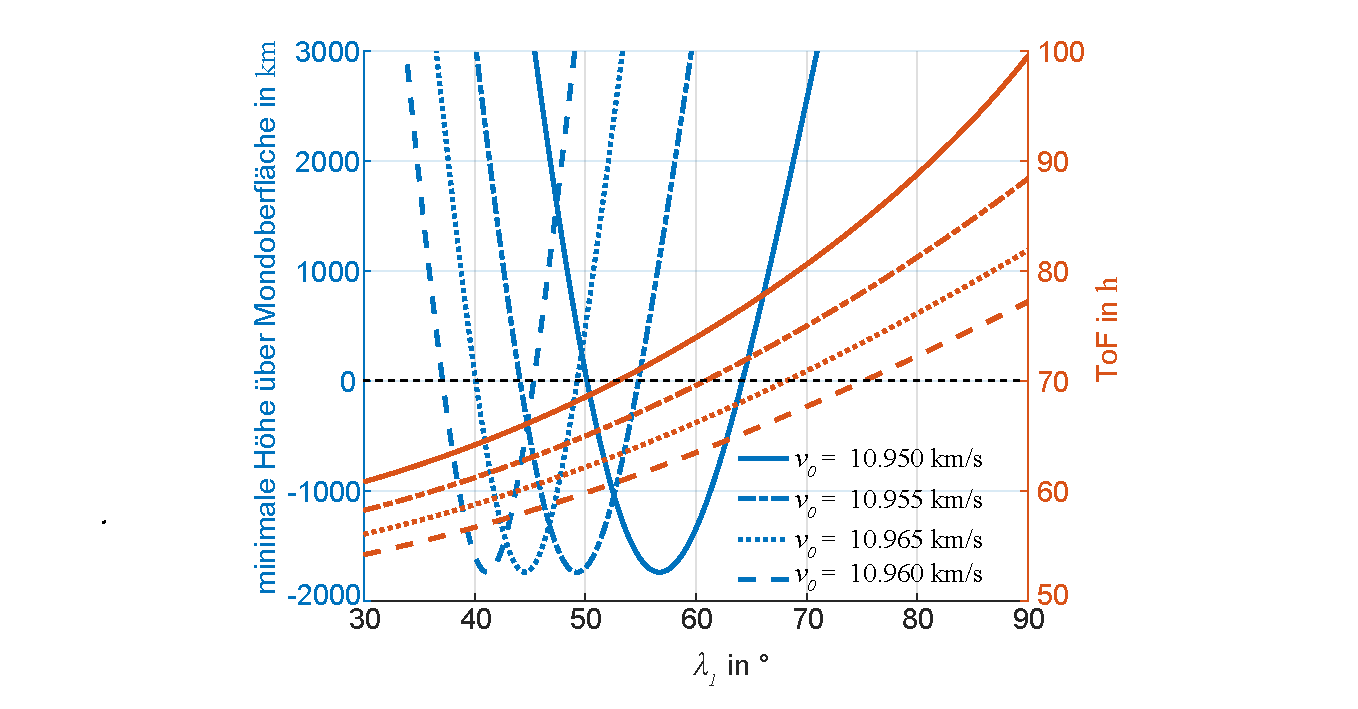
\includegraphics[width=\textwidth]{PatchConicApollo13.pdf} 
	\caption[Ergebnisse der \textit{Patch Conic} N�herung f�r Apollo 13.]{Ergebnisse der \textit{Patch Conic} N�herung f�r Apollo 13.}
	\label{abb:adyn_FRT06}
\end{figure}

Wir erhalten dann \zb f�r $v_0 = \SI{10960.0}{\km\per\second}$ in der
\textit{Patch Conic} N�herung:\\
\begin{align*}
	\lambda_1      &: 49.70\degree  && \\ 
	\varphi_0      &: 129.89\degree\\ 
	\mathrm{ToF} &: 78.7\,\mathrm{h}\\ 
	h_\text{P,M} &: \SI{279.3}{\km} \, 
\end{align*}
was schon relativ gut mit den tats�chlichen Werten von Apollo 13 �bereinstimmt, wobei man ber�cksichtigen muss, dass beim tats�chlichen Raumflug es eine Reihe von Kurskorrekturen gab.

In der numerische Betrachtung (L�sung der Bewegungsgleichungen) ergeben sich dann eine Vielzahl von L�sungen. Das liegt daran, dass es sich bei der Bestimmung der FRT ja um ein Optimierungsproblem handelt, bei dem $h_0$, $h_\text{Reentry}$ und $h_\text{P,M}$ gegeben sind und $v_0$ und $\varphi_0$ gesucht werden. F�r solche Optimierungsprobleme gibt es h�ufig keine eindeutigen L�sungen. Wir erhalten \zb f�r $v_0 = \SI{10960.0}{\km\per\second}$ und $\varphi_0 = 129.33\degree$:
\begin{align*}
	\mathrm{ToF}\, \text{zum Mond} &: 78.2\,\mathrm{h}\\ 
	\mathrm{ToF}\, \text{Gesamt} &: 156.4\,\mathrm{h}\\ 
	h_\text{M,P}\, \text{Mond} &: \SI{2111.0}{\km}\\
	h_\text{Reentry}\, \text{Erde} &: \SI{150.0}{\km} 
\end{align*}
Die L�sung ist im Detail im \mscr~\mladynref{FreeReturnTrajectoryApollo13.m} ausgef�hrt.\\

\subprob{Genauere Rechnungen f�r Apollo 13}

Bisher haben wir die Erde als ruhend angenommen und den Mond auf einer Kreisbahn um diese rotierend, Wir betrachten nun das vollst�ndige Dreik�rper-Problem Erde, Mond und Apollo 13 im Schwerpunktsystem von Erde-Mond. Wiederum handelt sich hierbei um ein Optimierungsproblem, bei dem $h_0$ und $h_\text{Reentry}$ gegeben sein sollen und $v_0$, $\varphi_0$ und $h_\text{P,M}$ gesucht werden.
Die Rechnungen ergeben in diesem Fall beispielhaft, 
\begin{align*}
	v_0      &: \SI{10963.0}{\km\per\second}\\ 
	\varphi_0      &: 130.46\degree\\ 
	\mathrm{ToF}\, \text{zum Mond} &: 75.2\,\mathrm{h}\\ 
	\mathrm{ToF}\, \text{Gesamt} &: 149.5\,\mathrm{h}\\ 
	h_\text{P,M}\, \text{Mond} &: \SI{1353.4}{\km}\\
	h_\text{Reentry}\, \text{Erde} &: \SI{169.6}{\km} \,,
\end{align*}
wobei wir hier vor darauf geachtet haben, dass der Wiedereintritt in die Erdatmosph�re gew�hrleistet ist, daf�r der Mondabstand etwas gr��er gew�hlt ist.
Das L�sungsbeispiel ist in \figref{adyn_FRT08} dargestellt und im Detail im \mscr~\mladynref{FreeReturnTrajectoryApollo13CoM.m} ausgef�hrt.\\

\begin{figure}[H]
	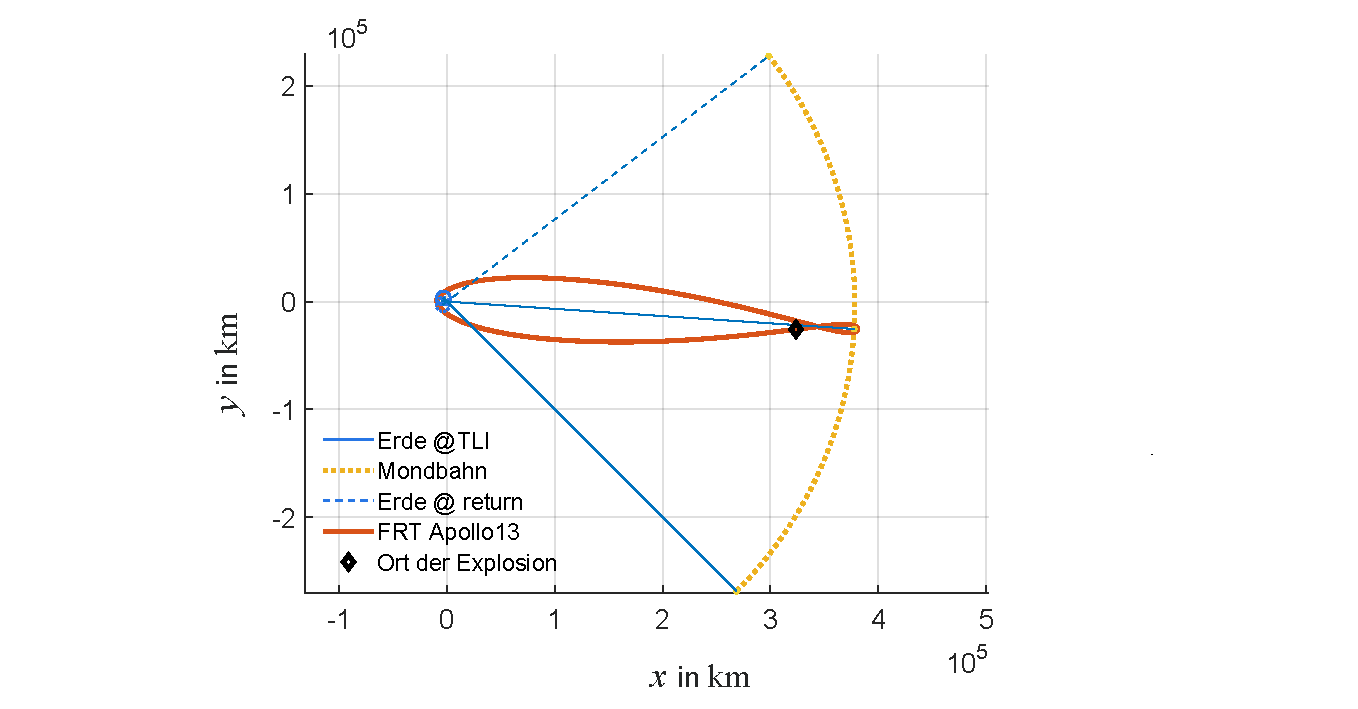
\includegraphics[width=\textwidth]{FRTApollo13.pdf} 
	\caption[Ergebnisse der numerischen Rechnung f�r eine \textit{Free Return Trajectory } f�r Apollo 13.]{Ergebnisse der numerischen Rechnung f�r eine \textit{Free Return Trajectory} im Schwerpunktsystem Erde-Mond. In der Graphik ist auch der Ort der Explosion des Tanksystems von Apollo 13 eingezeichnet.}
	\label{abb:adyn_FRT08}
\end{figure}

\newpage	
\subprob{Allgemeine Bemerkungen - Alternative Ans�tze}

Wie bereits erw�hnt, handelt es sich bei der Bestimmung der FRT um ein Optimierungsproblem. \cite{Battin1999, Brown2002, Bate1971, Vallado2007}. 
Bei der L�sung desselben findet man, dass die L�sungswerte $h_\text{P,M},\, h_\text{Reentry}$ sehr stark auf kleinere Ver�nderungen der Eingabeparameter variieren, \zb wird bei kleinsten �nderungen der Anfangsgeschwindigkeit (TLI-Geschwindigkeit) $v_0$ oder des TLI-Phasenwinkels $\varphi_0$ bei ansonsten festgehaltenen Parametern die Reentry-Flugbahn sehr stark variieren, was bedeuten k�nnte, dass das Raumschiff auf der FRT entweder in der Erdatmosph�re vergl�ht oder von dieser abprallt (siehe \kap{adyn_reentry}).\\
In der Realit�t wird man deswegen die Missionsplanung im Verlauf einer FRT mit kleineren Kurskorrekturen versehen, die wesentliche gr��ere Toleranzen der Parameter ($v_0$, $\varphi_0$) erlauben. Man kann in diesem Fall auch als weitere Randbedingung f�r die Optimierungsaufgabe einen minimalen Treibstoffverbrauch f�r die Summe der einzelnen Kurskorrekturen und Bahn�nderungen fordern, also f�r
\begin{align*}
    \Delta v_{\text{ges}} = \Delta v_{\text{TLI}} + \Delta_\text{Cor,E$\to$M} + \Delta v_{\text{LOI}} + \Delta v_{\text{TEI}} + \Delta_\text{Cor,M$\to$E} + \Delta v_{\text{EOI}}
\end{align*}
Hierbei bedeuten:
\begin{align*}
    \Delta_\text{Cor,E$\to$M} &: \text{Geschwindigkeitsbudget f�r Kurskorrektur auf dem We g $E \to M$ (\bzw $M \to E$)}\\
    \Delta v_\text{LOI,EOI} &: \text{Geschwindigkeitsbudget f�r Lunar Orbit Injektion \bzw Earth Orbit Injektion}\\
    \Delta v_{\text{TEI}} &: \text{Geschwindigkeitsbudget f�r Trans Earth Injektion}
\end{align*}
Dem interessierten Leser sei auf die Ref. \cite{Gagg2016} verwiesen, in welcher auch die einzelnen Schritte der mathematischen Optimierung\footnote{Die Optimierungsprobleme sind generell interessante mathematische Probleme, deren allgemeine Behandlung �ber den Umfang dieses Buches hinaus geht. Wir sind bereits bei der Herleitung der Lagrange-Gleichungen in Band I auf ein Problem dieser Art gesto�en und beim Lambert-Problem.} erl�utert sind.\\
Ebenso verweisen wir auf die unter \url{https://de.mathworks.com/matlabcentral/fileexchange} aufgef�hrten Programme  mit verschiedenen Optimierungsprozeduren in zum Teil vereinfachten Geometrien f�r die Berechnung der FRT.\footnote{ Wir verweisen insbesondere auf:\\
\url{Lunar Free-Return Trajectory Analysis with MATLAB - OTB - File Exchange - MATLAB Central (mathworks.com)},\\ \url{Lunar Free-Return Trajectory Analysis with MATLAB - File Exchange - MATLAB Central (mathworks.com)} und \\
\url{N-body Lunar Free Return Trajectory Analysis � OTB - File Exchange - MATLAB Central (mathworks.com)}.} \\

Wir wollen jedoch noch einen anderen Bezug herstellen. In Kap. 1.2.3.6 in Band I hatten wir das Drei-K�rper-Problem und insbesondere auch das sogenannte eingeschr�nkte Drei-K�rper-Problem eingef�hrt, bei welchem eine dritte Testmasse deutlich kleiner ist als die beiden anderen Massen. Bei dem FRT-Problem handelt es sich genau um ein solches Problem, welches wir im mitrotierenden \KOS (um den Schwerpunkt des Erde-Mond-Systems) wie folgt schreiben k�nnen (\vgl Gl. (1.100) in Band I), wobei wir die Striche f�r das mitbewegte System weglassen wollen. 
\begin{subequations}
\begin{align}
    \ddot{x}_\text{R} - 2\omega_\text{M}\,\dot{y}_\text{R}- \omega_\text{M}{}^2\,x_\text{R} &= -\frac{\mu_\text{E}}{r_{\text{RE}{}^3}}\,\lk x_\text{R} + m_\text{eff,M}\,r_{\text{EM}}\rk -\frac{\mu_\text{M}}{r_{\text{RM}{}^3}}\,\lk x_\text{R} - m_\text{eff,E}\,r_{\text{EM}}\rk\\
    \ddot{y}_\text{R} + 2 \omega_\text{M}\,\dot{x}_\text{R}  - \omega_\text{M}{}^2\,y_\text{R}  &= -\frac{\mu_\text{E}}{r_{\text{RE}{}^3}}\,y_\text{R} - \frac{\mu_\text{M}}{r_{\text{RM}{}^3}}\,y_\text{R}\,\label{eq:FRT_20}
\end{align}  
\end{subequations}
mit 
\begin{align*}
    r_\text{RE} = \left| \vec{r}_\text{R} - \vec{r}_\text{E} \right|, \quad
    r_\text{RM} = \left| \vec{r}_\text{R} - \vec{r}_\text{M} \right|, \quad
		m_\text{eff,E} = \frac{M_{\text{E}}}{M_{\text{E}} + M_{\text{M}}} \quad \text{und} \quad 
		m_\text{eff,M} = \frac{M_{\text{M}}}{M_{\text{E}} + M_{\text{M}}}\,.
\end{align*}
Setzt man die Anfangsbedingungen ($r_0, v_0$ \bzw $x_\text{R,0},y_\text{R,0},\dot{x}_\text{R,0},\dot{y}_\text{R,0}$) ein, erh�lt man als L�sung $\lk x_\text{R},y_\text{R}\rk$ die achtf�rmige Kurve nach \figref{adyn_FRT10}.

\begin{figure}[H]
	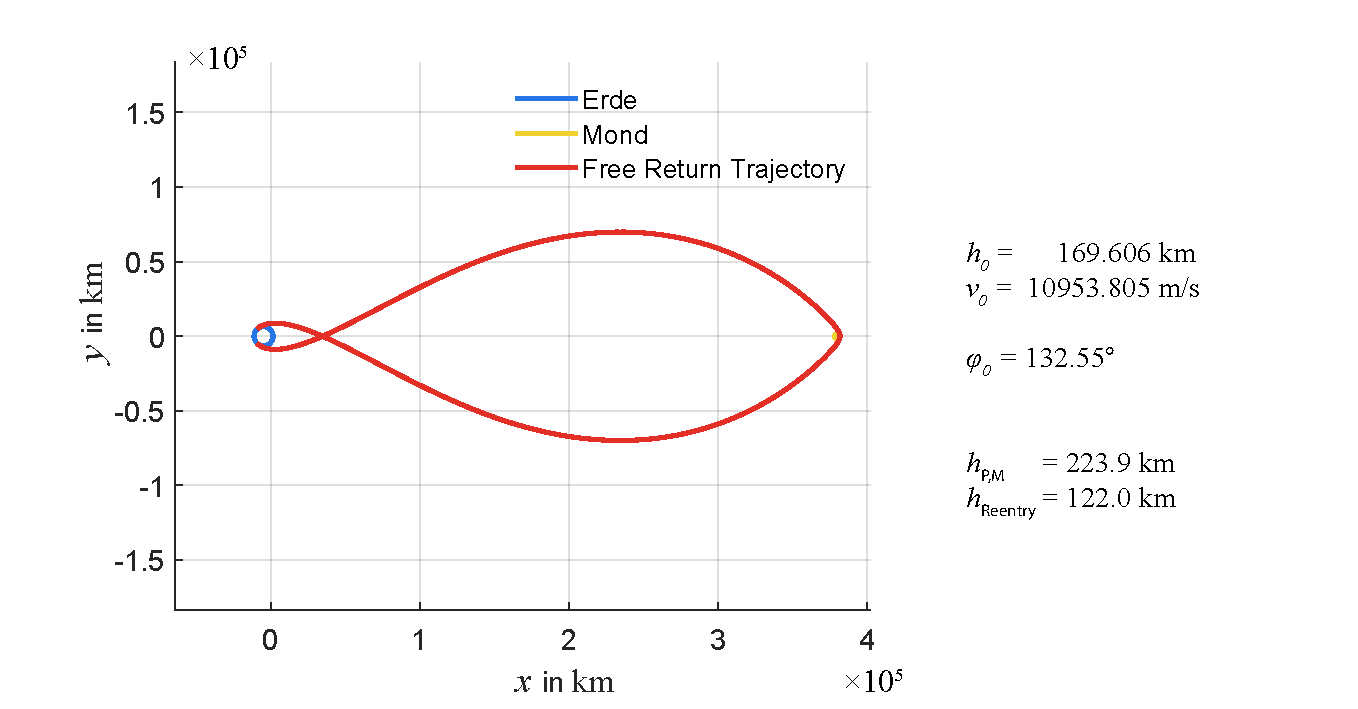
\includegraphics[width=\textwidth]{Transfer2MoonRotatingKOS.pdf} 
	\caption[Ergebnisse der numerischen Rechnung f�r das eingeschr�nkte Drei-K�rper-System Erde-Mond-Raumschiff.]{Ergebnisse der numerischen Rechnung f�r das eingeschr�nkte Drei-K�rper-System Erde-Mond-Raumschiff im mitrotierenden Koordinatensystem. Man beachte die unterschiedliche Form der Bahn, die wesentlich von der in \figref{adyn_FRT08} abweicht, was durch die unterschiedliche "`Perspektive"' des mitrotierenden Beobachters zustande kommt.}
	\label{abb:adyn_FRT10}
\end{figure}

Zum Schluss m�chten wir noch einmal bemerken, dass die FRT ein sch�nes Beispiel eines Swing-By-Man�vers (Gravity-Assist-Man�vers) (siehe \kap{adyn_gravity_assist}) beinhaltet und zwar ein Man�ver, bei welchem die Masse des Gravity-Assist-Himmelsk�rpers (in diesem Fall der Mond) abbremsend wirkt, da die Bahn nach \figref{adyn_swingby00} vor dem Himmelsk�rper liegt.

\end{subprobs}

\end{sol} 
\textcolor{blue} {$\rightarrow$ zur} \probref{adyn_rendezvous03}.\\
\noindent\rule[1ex]{\textwidth}{0.5pt}  \newpage  \clearpage

%-----------------------------------------------------------------------------------------------------------

\subsection{�bungen zu Starts aus der Erdatmosph�re und Wiedereintritt}

\noindent\rule[1ex]{\textwidth}{0.5pt} 

%-----------------------------------------------------------------------------------------------------------

\begin{sol}{prob:adyn_launch01a}\label{lsg:adyn_launch01a} %�bung25
\textbf{Bewegungsgleichungen f�r Raketenstart von Erdoberfl�che}\\

\begin{nebenrechnungNeu} {Nat�rliche Koordinaten}

(siehe \cite{Arens2008, Riley2006, Otto2019 })\\

Der zeitabh�ngige Einheitsvektor $\vec{t}$ der Tangente an die Bahnkurve (Tangentialvektor) ist definiert durch:
\begin{align}
    \vec{t} = \frac{\D \vec{r}}{\D s} ~~~\text{mit}~~~~\D s = | \D \vec{r}(t) | = \left| {\frac{\D \vec{r}}{\D t}} \right| \,  \D\,t= v(t)\; \D\,t\,,
\label{eq:adyn_NR_launch01}
\end{align}
worin $\D s$ die differentielle Bahnl�nge ist und $v$ der Betrag der Geschwindigkeit $\vec{v}$. Der Hauptnormalenvektor (ebenfalls eine Einheitsvektor) ist die 
normierte �nderung des Tangentialvektors �ber die Bahnl�nge:
\begin{align}
    \vec{n} = \frac{\D \vec{t}}{\D s} \big/ \left|\frac{\D \vec{t}}{\D s} \right|\,.
\label{eq:adyn_NR_launch02}
\end{align}
Aus $\vec{t}^2 =1 $ folgt $\D \vec{t} / \D s \cdot \vec{t} = 0$, \dh $\vec{n} \bot \vec{t}$, also $\vec{n} \cdot \vec{t} = 0$.
Damit kann man einen dritten Vektor definieren, der senkrecht auf dem Tangential- und dem Hauptnormalenvektor steht und Binormalvektor hei�t:
\begin{align}
    \vec{h} =  \vec{t} \times \vec{n}\,.
\label{eq:adyn_NR_launch03}
\end{align}
Die drei Vektoren $\vec{t},\,\vec{n},\, \vec{h}$ bilden ein (sogenanntes nat�rliches) Koordinatendreibein, das sich mit dem bewegten Objekt auf der Bahn mitbewegt und dabei sowohl einer Translation als auch Rotation unterliegt.
Die Geschwindigkeit $\vec{v}$ und die Beschleunigung $\vec{a}$ sind in diesen Koordianten dann definiert durch (\vgl Kap. 1.2.2. in Band I) 
\begin{align}
    \begin{split}
		    \vec{r} &=  v\,\vec{t}\\
        \vec{a} &=  \frac{\D}{\D t}\,\lk v\,\vec{t}\rk = \,\lek \dot{v}\,\vec{t} + v\,\dot{\vec{t}}\rek = \lek \dot{v}\,\vec{t} + v\,\vec{\omega}\times \vec{v}\rek\,.
    \end{split} \label{eq:adyn_NR_atmos03}
\end{align}
Hierin ist $\vec{\omega}$ die momentane Rotationsfrequenz des mitrotierenden \KOS definiert durch $\vec{t},\, \vec{n}$ und \vec{h}.\\

\end{nebenrechnungNeu}

Wir wollen zun�chst die momentane Rotationsfrequenz des nat�rlichen Dreibeins als Funktion von Bahnradius $r$ , Geschwindigkeit $v$ und FPA $\gamma$ berechnen. Wir betrachten dazu \figref{adyn_ueb_atmos01} und finden:
\begin{align}
    \vec{\omega} = \vec{\omega_1} + \vec{\omega_2} = (\omega_1 + \omega_2)\,\vec{h}\,,\label{eq:adyn_ueb_atmos05}
\end{align}
worin $\omega_1\,\vec{h}$ die Drehung durch die reine Bahnbewegung beschreibt und $\omega_2\,\vec{h}$ die Drehung des FPA ber�cksichtigt. Der Betrag von $\vec{\omega_1}$ ergibt sich aus \figref{adyn_ueb_atmos01} �ber $r\,\D\upsilon = |\D \vec{r}|\,\cos\gamma$ zu
\begin{align}
        \omega_1 = \dot{\upsilon} &= \frac{|\vec{v}|}{r}\,\cos\gamma = \frac{v}{r}\,\cos\gamma\, \label{eq:adyn_ueb_atmos05a} \,,
\end{align}
w�hrend der Betrag von $\vec{\omega_2}$ einfach der �nderungsrate des FPA entspricht (man beachte die Richtung!):
\begin{align}
        \omega_2 = - \dot{\gamma} \,.\label{eq:adyn_ueb_atmos05b}
\end{align}
Um die Bewegungsgleichung \eqref{eq:adyn_launch_vec},
\begin{align}
    m_\text{R}\lk t\rk \,\ddot{\vec{r}} = \vec{F}_\text{S}\lk t\rk + m_\text{R}\lk t\rk\,\vec{g}\lk \vec{r}\rk + \vec{F}_\text{D}\lk \vec{r},\dot{\vec{r}}\rk + \vec{F}_\text{A}\lk \vec{r},\dot{\vec{r}}\rk\, , \label{eq:adyn_ueb_atmos01}
\end{align}
in nat�rlichen Koordinaten schreiben zu k�nnen, schreiben wir die Kr�fte \bzw Beschleunigungen in \eqref{eq:adyn_ueb_atmos01} unter Ber�cksichtigung der Geometrie von \figref{adyn_launch02} in nat�rlichen Koordinaten (die Bewegung und alle Kr�fte sollen in einer Ebene liegen) und benutzen dabei den Angle of Attack $\alpha$ und den Flight Path Angle $\gamma$:
\begin{align}
\begin{split}
				\vec{F}_\text{S} &= F_\text{S}\,\cos\alpha\,\vec{t} + F_\text{S}\,\sin\alpha\,\vec{n}\,,~~~~\vec{F}_\text{A}  = F_\text{A}\,\vec{n}\,,~~~
        \vec{F}_\text{D} = -F_\text{D}\,\vec{t}\,,~~~\vec{g} = -g\,\sin\gamma\,\vec{t} -g\,\cos\gamma\,\vec{n}\,.
\end{split}\label{eq:adyn_ueb_atmos02}
\end{align} 
\begin{figure}[H]
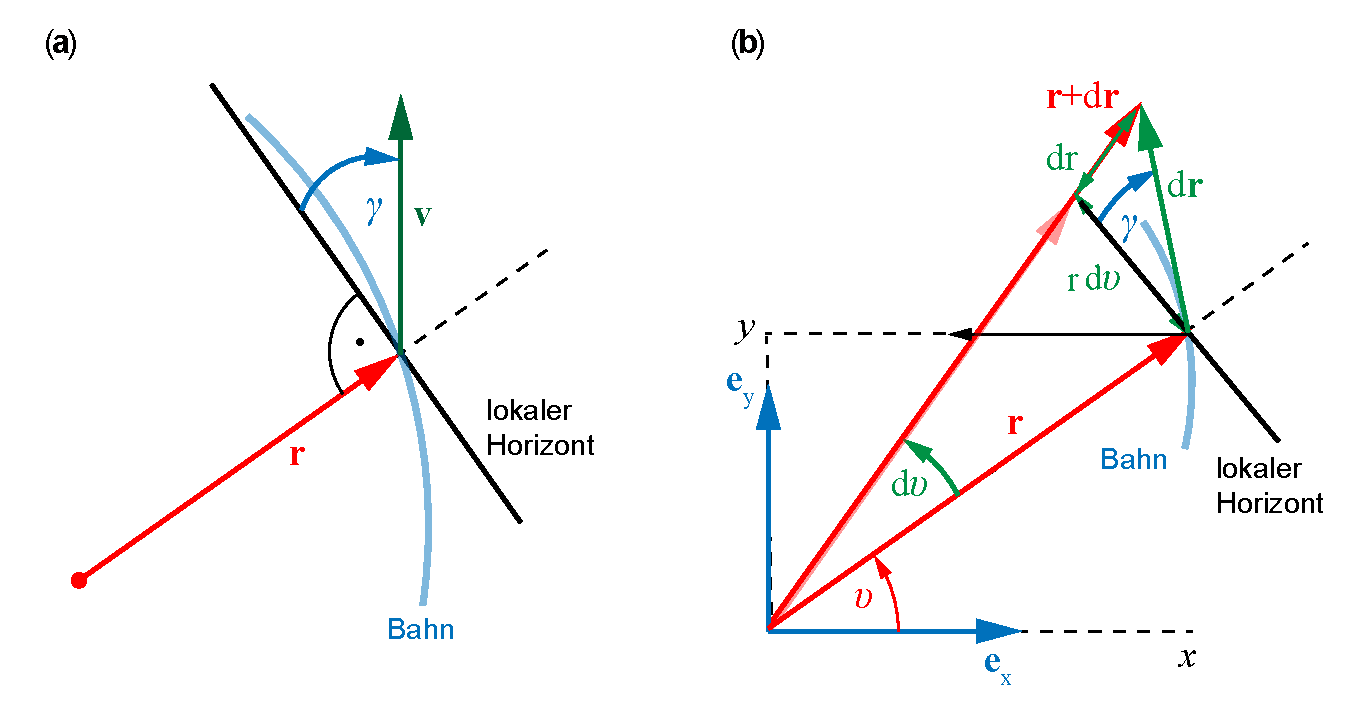
\includegraphics[width=\textwidth]{KOSReentry.pdf}
\caption[Zur Berechnung der Komponenten des Radialvektors einer Bahn im Inertialsystem der Erde.]{Zur Berechnung der Komponenten des Radialvektors einer Bahn im im Inertialsystem der Erde und im zylindrischen \KOS $\vec{t},\, \vec{n},\,\vec{h}$. \fa Lokaler Horizont, Geschwindigkeit und Flight Path Angle (FPA) $\gamma$. \fb Infinitesimale �nderungen von $r, \,\gamma$  und $v$. Der Winkel $\upsilon$ ist der Orbitalwinkel der Bahn (entspricht in etwa der wahren Anomalie) zwischen dem geozentrischen Ortsvektor zum Startpunkt und dem Ortsvektor zum Raumschiff zur Zeit $t$.}  

\label{abb:adyn_ueb_atmos01}
\end{figure}
Wir setzen \eqref{eq:adyn_ueb_atmos02} in \eqref{eq:adyn_ueb_atmos01} ein und erhalten eine Gleichung f�r $\vec{t}$ und $\vec{u}$.
\begin{align}
    \begin{split}
        \ddot{\vec{r}} &= \frac{\D}{\D t}\,\lk v\,\vec{t}\rk =  \lek \dot{v}\,\vec{t} + v\,\dot{\vec{t}}\rek = \lek \dot{v}\,\vec{t} + v \, \vec{\omega}\times \vec{v}\rek \\
        &= \lek \frac{F_\text{S}\,\cos\alpha - F_\text{D}} {m_\text{R}} \,- \,g\,\sin\gamma \rek\,\vec{t} + \lek \frac{F_\text{S}\,\sin\alpha + F_\text{A}}{m_\text{R}} - \,g\,\gamma\,\cos\gamma \rek\,\vec{n}\,.
    \end{split} \label{eq:adyn_ueb_atmos03}
\end{align}

Mit \eqref{eq:adyn_ueb_atmos05} - \eqref{eq:adyn_ueb_atmos05b} in \eqref{eq:adyn_ueb_atmos03} erhalten wir daraus jeweils eine Gleichung f�r $\vec{t}$ und 
$\vec{n}$, die jede f�r sich erf�llt sein muss, woraus folgt:
\begin{subequations}
    \begin{align}
        \dot{v}\,\vec{t} &= \lek \frac{F_\text{S}\,\cos\alpha-F_\text{D}}{m_\text{R}} - g\,\sin\gamma \rek\,\vec{t} \,, \\
        v\,\vec{\omega}\times \vec{v} &= \lk \dot{\theta}-\dot{\gamma}\rk\,\vec{h} \times v\,\vec{t}  = - \lek \frac{v^2}{r}\,\cos\gamma - v\, \dot{\gamma} \rek\,\vec{n} = \lek \frac{F_\text{S}\,\sin\alpha + F_\text{A}}{m_\text{R}} - \gamma\,g\,\cos\alpha \rek \,\vec{n}\,.
    \end{align} \label{eq:adyn_ueb_atmos04}
\end{subequations}

Nach einfacher Umformung erhalten wir schlie�lich die zwei verkoppelten skalaren Differentialgleichungen f�r $v$ und $\gamma$:
\begin{subequations}
    \begin{align}
        \dot{v} &= \frac{F_\text{S}\,\cos\alpha - F_\text{D}}{m_\text{R}} - g\,\sin\gamma\,,\\
        \dot{\gamma} &= \frac{F_\text{S}\,\sin\alpha + F_\text{A}}{v\,m_\text{R}} - \lk \frac{g}{v} -\frac{v}{r}\rk\,\cos\gamma\,~.
    \end{align}\label{eq:adyn_ueb_atmos06}
\end{subequations}

F�r den projizierten Kreisbogen $s(t)$, den das Raumschiff (eigentlich der Koordinatenursprung des mitbewegten \KOS) auf der Erdoberfl�che s(t) beschreibt, den Abstand des Raumschiffs vom Erdmittelpunkt  $r$ \bzw seine H�he $h$ �ber der Erdoberfl�che finden wir leicht aus geometrischen �berlegungen (\figref{adyn_launch02} und \figref{adyn_ueb_atmos01}):

\begin{subequations}
    \begin{align}
        \dot{h} &= v\,\sin\gamma\,,\\ 
        \dot{s} &= \frac{R_\text{E}}{r}\,v\,\cos\gamma \,=\, \frac{1}{1+h/R_\text{E}}\,v\,\cos\gamma  \,.
    \end{align}\label{eq:adyn_ueb_atmos07}
\end{subequations}

Das Differential-Gleichungssystem \eqref{eq:adyn_ueb_atmos06} und \eqref{eq:adyn_ueb_atmos07} bestimmt damit vollst�ndig die Aufstiegsbahn im mitbewegten KOS. Diese Bahn liegt in der durch die Richtungen von $s$ und $h = r - R_\text{E}$ bestimmten Ebene. 

\end{sol} 
\textcolor{blue} {$\rightarrow$ zur} \probref{adyn_launch01a}.\\
\noindent\rule[1ex]{\textwidth}{0.5pt}  \newpage  \clearpage
%-----------------------------------------------------------------------------------------------------------

\begin{sol}{prob:adyn_launch01}\label{lsg:adyn_launch01} %�bung26
\textbf{Raketenstart von verschiedenen Weltraumzentren}\\

\begin{subprobs}
\subprob{Allgemeine Betrachtungen}

\begin{figure}[H]
	\includegraphics[width=\textwidth]{Aufstiegsbahnen.pdf} 
	\caption[Transfer eines Raumschiffs von der Erdoberfl�che in einen Erdorbit �ber eine Hohmann-Ellipse.]{Transfer eines Raumschiffs von der Erdoberfl�che in einen Erdorbit �ber eine Hohmann-Ellipse. \fa idealisierter Fall ohne Reibung \fb realistischer Fall bei Vorhandensein einer Atmosph�re. Im idealisierten Fall w�rde man die Rakete horizontal direkt in die Hohmann-Ellipse starten lassen, im Fall \fb aus aerodynamischen und strukturellen senkrecht zum Horizont und f�hrt dann eine Nickkorrektur aus, um das Raumschiff einen \textit{Gravitation Turn}\index{Gravitation Turn}\index{Schwerkraftdrehung}  machen zu lassen. Siehe unten im Text.}
	\label{abb:adyn_launch_lsg_Schema}
\end{figure}

Wir k�nnen die Berechnungen vorteilhafter weise im in \kap{adyn_launch} eingef�hrten mitbewegten \KOS tun, da es uns nur um die Dynamik und nicht um eine geographische Berechnung der Bahn geht.\\
Zielstellung der Berechnung ist, das Raumschiff in eine Kreisbahn mit der H�he $h_\text{K}$ (numerische Werte beispielhaft f�r $h_\text{K}= \SI{300}{\km}$) zu bringen.\\
Ohne Atmosph�re w�rde man das Raumschiff horizontal in Richtung Osten von der Erde starten lassen (\figref{adyn_launch_lsg_Schema}a  und zwar mit einem Geschwindigkeitsbudget von
\begin{align}
	\Delta v_0 = \sqrt{\frac{G\,M_\text{E}}{R_\text{E}+h}} - \Delta v_\text{E,t} = \sqrt{\frac{G\,M_\text{E}}{R_\text{E}+h}} - \frac{2\pi\,R_\text{E}\,\cos\varphi_0}{\SI{86125}{\second}}\approx \SI{7.7309}{\km\per\second} - \SI{0.465}{\km\per\second}\,\cos\varphi_0 \,,
\end{align}
worin $\varphi_0$ die geographische Breite des Abschussortes ist und $\Delta v_\text{E,t}$ die Tangentialgeschwindigkeit auf der Erdoberfl�che der Erdrotation bezeichnet.
Das Raumschiff bewegt sich in diesem idealisierten Fall auf einer Hohmann-Ellipse (\kap{adyn_hohmann_transfer}) mit der Halbachse $a_\text{T}$ und der Exzentrizit�t $e_\text{T}$ (Numerische Werte f�r $h=\SI{300}{\km}$.)
\begin{align*}
	a_\text{T} &= \frac{1}{2} \, \lk R_\text{E} + h + R_\text{E} \rk = R_\text{E}+\frac{h}{2} \approx \SI{6528}{\km} \,,\\
  e_\text{T} &= \frac{h}{2R_\text{E}+h } \approx 0.022978\,.
\end{align*}
und br�uchte 
\begin{align}
	t_\text{f} = t_\text{T}= \pi\sqrt{\frac{a_\text{T}{}^3}{G\,M_\text{E}}} \approx \SI{43.5}{\minute}\,,
\end{align}
um in die Umlaufbahn zu gelangen, wo noch einmal entsprechend Gleichung \eqref{eq:adyn_hohmann04} ein Burn notwendig ist, um das Raumschiff aus der elliptischen Bahn in die Kreisbahn zu bringen.\\
In einem realistischen Fall (\figref{adyn_launch_lsg_Schema}b, \dh unter Ber�cksichtigung von Drag, wird das Raumschiff nach der Schubphase zum Zeitpunkt $t_\text{T}$ an einem �bergangspunkt T auf die Hohmann-Ellipse treffen. Dort m�ssen dann folgende Bedingungen erf�llt sein:\footnote{Hierbei haben wir die Gleichungen \eqref{eq:adyn_reentry02} benutzt. Wir hatten ja in \kap{adyn_reentry} darauf hingewiesen, dass diese Gleichungen sowohl f�r den De-Orbit als auch die Startphase gelten.}
\begin{subequations}
\begin{align}
    \cos\gamma_\text{T} &= \cos\gamma(t_\text{T})=\frac{1+e_\text{T}\,\cos\upsilon_\text{T}}{\sqrt{1+2e_\text{T}\,\cos\upsilon_\text{T} +e_\text{T}{}^2}}\,,\label{eq:adyn_launch_lsg01a}\\
    v_\text{T} &= v(t_\text{T}) = \sqrt{\frac{G\,M_\text{E}}{a_\text{T}(1-e_\text{T}{}^2}}\,\sqrt{1+2e_\text{T}\,\cos\upsilon_\text{T}+e_\text{T}{}^2} \label{eq:adyn_launch_lsg01b} \,,\\
    h_\text{T} &= r(t_\text{T}) - R_\text{E} = \frac{a_\text{T}\,\lk 1-e_\text{T}{}^2\rk}{1+e_\text{T}\,\cos\upsilon_\text{T}} - R_\text{E}\,.\label{eq:adyn_launch_lsg01c}
\end{align} \label{eq:adyn_launch_lsg01}
\end{subequations}

Hierin ist $\gamma_\text{T}$ der FPA und $\upsilon_\text{T}$ die wahre Anomalie der Hohmann-Ellipse zum Zeitpunkt $t_\text{T}$.\\
F�r den Startzeitpunkt $t=0$ gilt:
\begin{subequations}
\begin{align}
    \gamma_0 &= \gamma(t = 0)=  \pi/2 \label{eq:adyn_launch_lsg02a}\,,\\
    v_0 &= v(t=0) = 0 \label{eq:adyn_launch_lsg02b} \,,\\
    h_0 &= h(t=0) = 0 \,.\label{eq:adyn_launch_lsg02c}
\end{align} \label{eq:adyn_launch_lsg02}
\end{subequations}

Die Schubphase muss also durch geeignete Steuerung des Anstellwinkles (AoA) $\alpha(t)$, der Massenverlustrate $\dot(m)(t)$, des Schubs $F_\text{S}(t)$ und der Wahl von $\upsilon(t)$ so gestaltet werden, dass als Ergebnis der zeitlichen Entwicklung des DGL-Systems \eqref{eq:adyn_launch01} die Bedingungen \eqref{eq:adyn_launch_lsg01} erf�llt werden und dies bei m�glichst geringem Treibstoffverbrauch \bzw gro�er Nutzlast. Wir wissen nun aus \kap{adyn_launch}, Gleichung \eqref{eq:adyn_launch07}, dass ein AoA verschieden von Null zu Verlusten zus�tzlich zu den unvermeidlichen Gravitations- und Reibungsverlusten f�hrt. Andererseits zeigt die formale Integration von \eqref{eq:adyn_launch01} auch, dass ein $\alpha$ verschieden von Null zu einer gew�nschten Ver�nderung des FPA f�hrt.
\begin{subequations}
\begin{align}
    v(t_\text{T}) &= \int\limits_0^{t_\text{T}} \frac{F_\text{S}}{m_\text{R}}\,\D t' - \underbrace{\int\limits_0^{t_\text{T}} \frac{F_\text{D}}{m_\text{R}}  \,\D t'}_{\mathrm{Reibungsverlust}} - \underbrace{\int\limits_0^{t_\text{T}} \frac{F_\text{S}\,(1-\cos\alpha)}{m_\text{R}}  \,\D t'}_{\mathrm{Steuerungsverlust}}  - \underbrace{\int\limits_0^{t_\text{T}} g\,\sin\gamma \,\D t'}_{\mathrm{Gravitationsverlust}} \label{eq:adyn_launch_lsg03a} \,, \\
    \gamma(t_\text{T}) &= \frac{\pi}{2}+ \underbrace{\int\limits_0^{t_\text{T}} \frac{F_\text{S}\,\sin\alpha}{m_\text{R}\,v}  \,\D t'}_{\mathrm{Steuerungsverlust}} -  - \underbrace{\int\limits_0^{t_\text{T}}\frac{g}{v}\,\cos\gamma \,\D t'}_{\mathrm{Gravitationsverlust}} + \underbrace{\int\limits_0^{t_\text{T}}\frac{v}{r}\,\cos\gamma \,\D t'}_{\mathrm{Zentrifugalgewinn}} \nonumber \\
		&= \frac{\pi}{2} + \underbrace{\int\limits_0^{t_\text{T}} \frac{F_\text{S}\,\sin\alpha}{m_\text{R}\,v}  \,\D t'}_{\mathrm{Steuerungsverlust}} - \underbrace{\int\limits_0^{t_\text{T}} \lk \frac{g}{v} - \frac{v}{r} \rk \,\cos\gamma  \,\D t'}_{\mathrm{Gravitation~Turn}} \,. \label{eq:adyn_launch_lsg03b}
\end{align} \label{eq:adyn_launch_lsg03}
\end{subequations}

Das erscheint zun�chst wie ein Dilemma, denn erreicht man eine gro�e �nderung von $\gamma$, verliert man an Geschwindigkeit $v$. Zum Gl�ck gibt es, wie man am 2. Term in \eqref{eq:adyn_launch_lsg03b} sieht, den \textit{Gravitation Turn} (in etwa Schwerkraftdrehung), der sich aus der Kombination von Schwerkraft und Zentrifugalkraft\footnote{Da wir die Gleichungen \eqref{eq:adyn_launch01} im mitbewegten \KOS geschrieben haben tritt in diesen die Zentrifugalkraft auf.} f�r $\gamma \neq \pi/2$ ergibt und der automatisch Null wird, wenn $v$ gegen die Kreisbahngeschwindigkeit $\sqrt{g\,r}$ geht. Der Vorteil der Schwerkraftdrehung besteht darin, dass der Schub nicht dazu verwendet werden muss, um die Richtung des Raumfahrzeugs zu �ndern, und noch wichtiger, dass w�hrend der anf�nglichen Aufstiegsphase die Rakete eine Anstellwinkle von Null behalten kann, welcher die aerodynamischen Belastungen der Rakete erheblich reduziert.\\
Wie findet nun ein Raketenstart unter Nutzung der Schwerkraftdrehung statt?  Nach dem vertikalen Start gewinnt die Rakete zun�chst an Vertikalgeschwindigkeit und H�he. W�hrend dieses Teils des Starts wirkt der Schwerkraftwiderstand, der in der n�chsten Phase des Starts mit dem sogenannten Pitchover-Man�ver (Nick-Korrektur) reduziert wird.\footnote{Die Nick-Korrektur wird bei immer noch relativ geringen Vertikalgeschwindigkeiten durchgef�hrt, um aerodynamische Belastungen auf das Raumschiff zu vermeiden. Der Neigungswinkel des Pitchover-Man�ver betr�gt nur wenige Grad, es gibt aber auch F�lle, bei denn relativ gro�e Winkel (einige zehn Grad) verwendet werden. Die Nickkorrektur dauert \ia nur sehr kurz und ist der einzige Moment w�hrend der Aufstiegsphase, in dem der Schub zum Lenken genutzt wird. Nach dem Pitchover-Man�ver bleibt der AoA f�r den Rest des Aufstiegs bei Null, so dass auch der Auftrieb vernachl�ssigt werden kann.}
Das Pitchover-Man�ver dient zwei Zwecken. Erstens dreht es die Rakete leicht, so dass ihre Flugbahn nicht mehr vertikal verl�uft, und zweitens bringt es die Rakete auf den richtigen Kurs (Startazimut)\index{Startazimut} f�r ihren Aufstieg in die Umlaufbahn. Siehe dazu auch den folgenden L�sungsteil zum Startfenster (Launch Window) und  Startrichtung (Startazimut)). 

\subprob{Startphase einer dreistufigen Rakete (Ariane-1) im $\vec{t},\, \vec{n}$ und \vec{h} - \KOS.}

Im \mscr~\mladynref{Raketenstart2Orbit01.m} und \mladynref{Raketenstart2Orbit02.m} berechnen wir die f�r eine dreistufige Rakete den Transfer in den erdnahem Orbit.

\begin{figure}[H]
	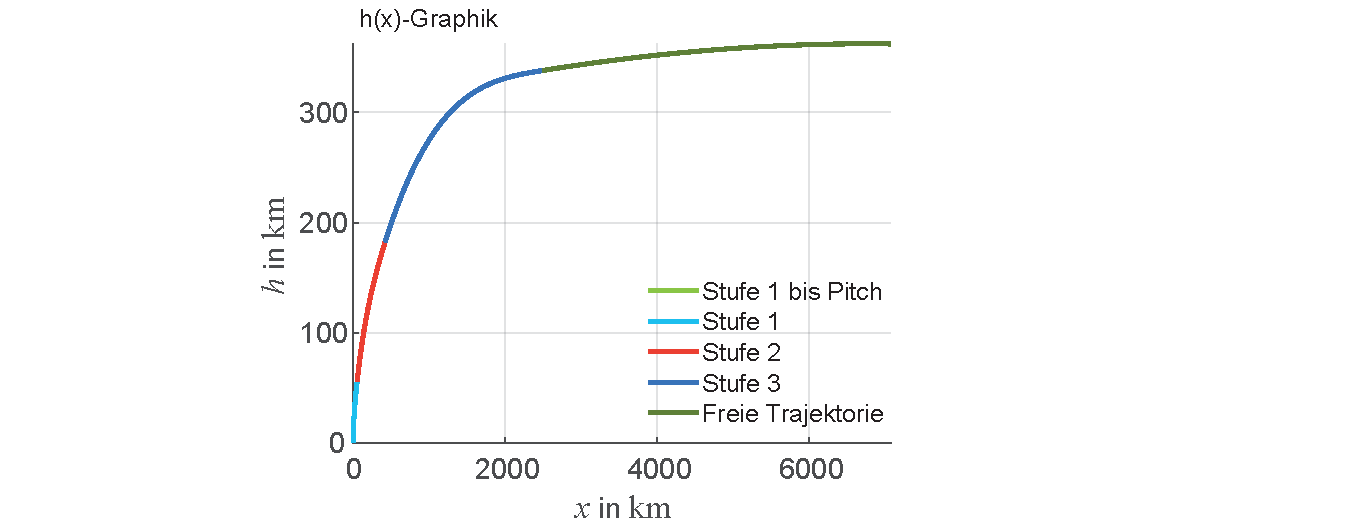
\includegraphics[width=\textwidth]{Startkurve.pdf} 
	\caption[Trajektorie nach Start von der Erdoberfl�che.]{Trajektorie nach Start von der Erdoberfl�che. Parameter siehe \mladynref{Raketenstart2Orbit02.m}.}
	\label{abb:adyn_launch_lsg02}
\end{figure}

\begin{figure}[H]
	\includegraphics[width=\textwidth]{Raketenstart2OrbitUebersicht.pdf} 
	\caption[Geschwindigkeit, Bahnh�he, FPA und Masse nach Start von der Erdoberfl�che. ]{Geschwindigkeit, Bahnh�he, FPA und Masse nach Start von der Erdoberfl�che f�r eine dreistufige Rakete bis zum �bergangspunkt (hier mit $h_\text{T} = \ca \SI{350}{\km}$ angenommen. Parameter siehe \mladynref{Raketenstart2Orbit02.m}.}
	\label{abb:adyn_launch_lsg03}
\end{figure}

\subprob{Startfenster (Launch Window) und  Startrichtung (Startazimut)}

Bisher haben wir uns nur mit der Dynamik und den energetischen Fragen eines Starts von der Erdoberfl�che und des anschlie�enden Transfer in eine gew�nschte Umlaufbahn besch�ftigt, nicht aber mit den Fragen nach der Zeit und den r�umlichen-geometrischen Bedingungen. Man k�nnte nat�rlich prinzipiell das Raumschiff zu jedem beliebigen Zeitpunkt starten und es auch an einen beliebigen Ort schie�en, um dann mit verschiedenen Bahnman�ver die Zielbahn zu erreichen. Aber das w�re eine enorme Verschwendung von Treibstoff. 

Unter einem Startfenster verstehen wir den Zeitraum, in welchem ein Raumschiff direkt in den gew�nschten Orbit \bzw auf eine geeignete Transferbahn (siehe vorhergehenden Abschnitt) gestartet werden kann. Dazu m�ssen wir abh�ngig vom gew�nschten Orbit und der geographischen Position des Abschussortes eine geeignet Startzeit und einen geeigneten Startwinkel finden. 

Hierbei gilt es zwei F�lle zu unterscheiden, zum einen, wenn die Inklination der gew�nschten Bahn $i$ gr��er oder gleich der geographischen Breite $\varphi_0$ des Startplatzes ist und zum anderen, wenn die Bahnneigung kleiner als die geographischen Breite ist. Wir werden sehen, dass es im zweiten Fall M�glichkeit gibt, direkt in den Orbit zu starten. 

Ein geeigneter Startzeitpunkt ist gegeben, wenn sich der Startort in der Position der Sternzeit des Startfensters (LWST) befinden, wobei  �in Position� hei�t, dass sich  Startplatz (bzw genauer der Breitenkreis des Startorts) und die gew�nschte Bahnebene schneiden. Wir betrachten dazu das sph�rische Dreieck in \figref{adyn_launch_lsg02}, welches durch drei Linien/Seiten gegeben ist. Die erste Seite ergibt sich aus der Bodenspur f�r die Umlaufbahn, die zweite aus der �quatorlinie und die dritte aus dem L�ngenkreis des Startplatzes. 
Aus \figref{adyn_launch_lsg02} entnehmen wir ferner noch weitere Gr��en mit folgenden Definitionen und Beziehungen:\\

\begin{tabular}[h]{ll}
LWST &~Sternzeit des Startfenster\index{Startfenster} (Launch Window Siderial Time)\index{Launch Window Siderial Time}\\
$\delta$ &~Hilfswinkel in Startrichtung\\
$\theta$ &~Standortwinkel des Startfensters\\
$\beta$  &~Startazimut\index{Startazimut}\\
$\Omega$ &~Rektaszension des aufsteigenden Knotens\\
\end{tabular}

\begin{figure}[H]
	\includegraphics[width=\textwidth]{BestimmungLWST.pdf} 
	\caption[LST und sph�risches Dreieck zur Bestimmung des LWST.]{LST \fa und sph�risches Dreieck zur Bestimmung des LWST \fb.}
	\label{abb:adyn_launch_lsg04}
\end{figure}

Mit dem Winkelkosinussatz der sph�rischen Trigonometrie \cite{Meyers1995} $~\cos \alpha = -\cos\beta\,\cos\gamma\,+\,\sin\beta\,\sin\gamma\,\cos a$ 
finden wir 
\begin{align*}
\cos i = -\cos(\pi/2)\,\cos\delta\,+\,\sin(\pi/2)\,\sin\delta\,\cos \varphi_0\,,
\end{align*}
was sich mit $\cos(\pi/2) = 0$ und $\sin(\pi/2) = 1$ zu
\begin{align}
\sin \delta = \cos i / \cos \varphi_0\, \label{eq:adyn_launch_lsg04}
\end{align}
vereinfacht. F�r das rechtwinklige sph�rische Dreieck gilt au�erdem \cite{Meyers1995}: $\cos \delta = \cos \theta \,\sin i~$, 
woraus schlie�lich mit \eqref{eq:adyn_launch_lsg03}
\begin{align}
\cos \theta = \frac{\cos \delta }{\sin i} = \frac{\sqrt{1 - \sin^2\delta}}{\sin i} = \frac{\sqrt{\lk 1 - \cos^2 i / \cos^2 \varphi_0 \rk}}{\sin i}
\label{eq:adyn_launch_lsg05}
\end{align}
folgt. F�r die n�rdliche Hemisph�re ergibt sich damit das LWST zu:
\begin{align}
\text{In der N�he des aufsteigenden Knotens: ~~~}\mathrm{LWST}_\text{auf} &= \Omega + \theta ~\,, \label{eq:adyn_launch_lsg06} \\
\text{In der N�he des absteigenden Knotens: ~~~~}\mathrm{LWST}_\text{abs} &= \Omega + (180\degree - \theta) \,. \label{eq:adyn_launch_lsg07}
\end{align}

\begin{figure}[H]
	\includegraphics[width=\textwidth]{StartAzimute.pdf} 
	\caption[Startazimut.]{Startazimut in der N�he des \fa aufsteigenden Knotens und des \fb absteigenden Knotens.}
	\label{abb:adyn_launch_lsg05}
\end{figure}

Es gibt noch einen letzten Winkel, der ber�cksichtigt werden muss, n�mlich das Startazimut $\beta$, \dh die Richtung in die gestartet werden soll. Dies ist der Winkel zwischen dieser �Aufw�rts�-Richtung und der Startrichtung (\figref{adyn_launch_lsg03}) und wird von der Nordrichtung aus im Uhrzeigersinn gemessen. Er ist vom Betrag her gleich dem Winkel $\delta$, womit wir schreiben k�nnen:
\begin{align}
\beta = \arcsin \frac{\cos i}{\cos \varphi_0}\,. \label{eq:adyn_launch_lsg08}
\end{align}
Wir erkennen an dieser Beziehung auch, dass die erreichbare Neigung der Bahn immer gr��er als die geographische Breite des Startortes sein muss, andernfalls w�rde $\beta$ komplexe Werte annehmen. Es gilt also immer $i \geq \varphi_0$, wobei die minimal Bahnneigung bei einem Startazimut von $90\degree$ (entspricht Ost) erreicht wird (\figref{adyn_launch_lsg04}).\\
F�r ein gegebenes $\Omega$ der Bahn gibt es  zwei L�sungen oder Startzeiten pro Rotation. Bei jeder davon kann man dann zwischen prograden und retrograden Umlaufbahnen w�hlen. Diese werden entlang der berechneten Startazimute in Richtung Norden oder S�den verlaufen, wobei die Startfenster einige Zeit auseinander liegen. Es gibt nur eine L�sung, wenn die Neigung genau dem Breitengrad entspricht.  Wir wolle zwei Beispiele angeben (siehe auch \mscr~\mladynref{Raketenstart2Orbit03.m}).

\begin{figure}[H]
	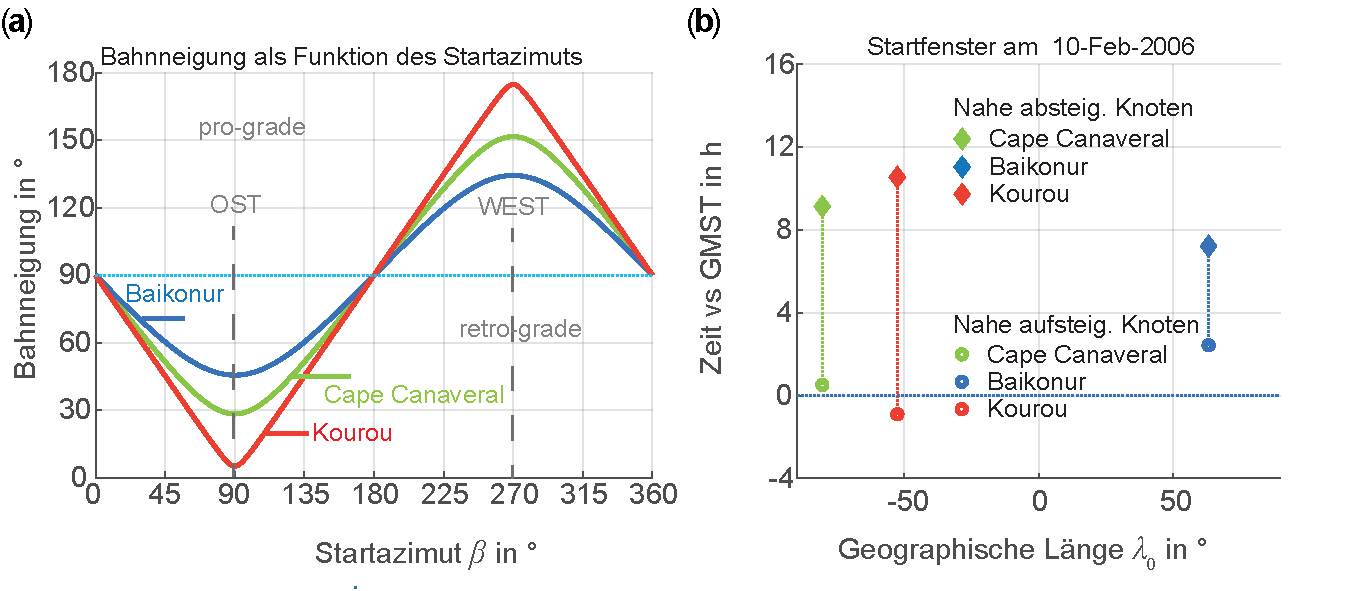
\includegraphics[width=\textwidth]{StartAzimuteStartFenster.pdf} 
	\caption[Bahnneigung und Startfenster als Funktion des Startazimuts und Startfenster zur ISS.]{Bahnneigung \fa und Startfenster \fb als Funktion des Startazimuts f�r verschiedene Weltraumzentren.}
	\label{abb:adyn_launch_lsg06}
\end{figure}

Die Internationale Raumstation umkreist die Erde mit einer Neigung von $51.6\degree$. F�r einen Start von Cape Canaveral (Breitengrad $28.383\degree$) \bzw vom Kosmodrom Baikonur (Breitengrad 45.617�) in die ISS-Umlaufbahn berechnen sich die Startazimute zu:
ergibt sich dann:
\begin{align*}
\beta_\text{CC}  &= \arcsin \frac{\cos(51.6\degree)}{\cos(28.383\degree)} = 44.98\degree~~ \text{\bzw}~~135.02\degree\,,\\ 
\beta_\text{Bai} &= \arcsin \frac{\cos(51.6\degree)}{\cos(45.617\degree)} = 63.21\degree~~ \text{\bzw}~~116.80\degree\,. 
\end{align*}

Die Berechnung der  Startfenster und Startazimute f�r die ISS f�r den 10. M�rz 2006 ist im \mscr~\mladynref{Raketenstart2Orbit03.m}\, ausgef�hrt.
F�r die ISS haben wir daf�r folgende Bahnparameter f�r Anfang 2006 benutzt \cite{JPL2020}.\\

\begin{tabular}{L{7cm}C{2cm}L{4cm}}
Epoche & $t_\text{epoch}$ & 09.02.2006 20:26:00.0000\\
Inklination &$i$ & $51.6448\degree$\\
Rektaszension des aufsteigenden Knotens & $\Omega$ & $122.3522\degree$\\
numerische Exzentrizit�t der Umlaufbahn & $e$ & 0.0008835\\
Argument des Perig�ums & $\omega$ &$257.3473\degree$\\
Mittlere Anomalie & $M$ & $251.7436\degree$\\
Mittlere Bewegung & $n$ & $ \SI{15.74622749}{\per\day}$\\
\end{tabular}
\medskip

Die Sternzeit in Greenwich bestimmt man aus dem Julianischen Datum JD f�r den Zeitpunkt 0:00 h UTC. Zun�chst berechnet man das Julianische Datum in Jahrhunderten seit dem 1.1.2000. 
	\[ T\,=\,\frac {JD-2451545.0}{36525} \]
und daraus die mittlere Sternzeit f�r Greenwich f�r den Zeitpunkt 0:00 h UTC:
\begin{align}
\mathrm {GMST_0} \,&=\,6^{\mathrm {h} }41^{\mathrm {m} }50.54841^{\mathrm {s}}\,+\,8640184.812866^{\mathrm {s} }\, T\,+\,0.093104^{\mathrm {s} }\, T^{2}\,-\,0.0000062^{\mathrm {s} }\, T^{3}\\
&=\,24110.54841^{\mathrm {s} }+8640184.812866^{\mathrm {s} }\, T \, + \,0.093104^{\mathrm {s} }\, T^{2}\,-\,0.0000062^{\mathrm {s} }\, T^{3}\\
&=\,100.46061837\degree+36000.770053608\degree\, T\,+\,0.000387933\degree\, T^{2}\,-\,(T^{3}/38710000)\degree
\end{align}
F�r einen Beobachter auf der geographischen L�nge $\lambda_0$ muss man die Sternzeit noch auf seine Ortssternzeit LST umrechnen:
\begin{align}
\mathrm {LST} \,&\,=\mathrm {GMST} +\lambda~~~{\text{f�r GMST im Gradma�}}
\end{align}

Wir verweisen auf das \mscr~\mladynref{Raketenstart2Orbit03.m} und auch auf \kap{hm_zeitdefinition}.


\subprob{Berechnung der 3D-Trajektorien im Inertialsystem}


F�r die weiteren Berechnungen muss man ber�cksichtigen, das wir alle Gr��en wie \zb das in \eqref{eq:adyn_launch_lsg08} abgeleitete Startazimut im Inertialsystem berechnet hatten. Da wir jedoch die Rakete von der rotierenden Erdoberfl�che starten, muss man die Erddrehung entsprechend ber�cksichtigen, was zu einer leichten Korrektur des Startazimuts und auch des Geschwindigkeitsbudgets f�hrt. Wir wollen ab sofort zur besseren Unterscheidung die Gr��en im mitbewegten System gestrichen kennzeichnen, die im Inertialsystem als ungestrichen.
So ist \zb f�r eine Umlaufbahn von 300 km H�he das Mindestgeschwindigkeitsbudget $\Delta \vec{v}$ (ohne Reibung und Reserven) durch $\Delta \vec{v} = \Delta v\,(\sin \beta\,\veceX + \cos \beta\,\veceY)$ mit $\Delta v = \SI{7.7309}{\km\per\second}$ gegeben, wobei die Einheitsvektoren in der Bahnebene liegen und in die Ost- \bzw Nordrichtung zeigen. Am einfachsten macht man sich nun an Hand von \figref{adyn_launch_lsg07} klar, dass zur Berechnung des Geschwindigkeitsbudget $\Delta \vec{v}'$ im Nichtinertialsystem die vektorielle Differenz von $\Delta \vec{v}$ und $\Delta v_\text{E,t}\,\veceX = \SI{0.465}{\km\per\second}\,\cos\phi_0$ (\vgl \eqref{eq:adyn_launch10}) gebildet werden muss. Man erh�lt:
\begin{align}
\Delta v' = \Delta v \, \sqrt{\lk \sin \beta \, - \Delta v_\text{E,t}/ \Delta v \rk^2 + \cos^2 \beta}\,. \label{eq:adyn_launch_lsg09}
\end{align}
Das Startazimut im mitbewegten System $\beta'$ ergibt sich dann zu:
\begin{align}
\beta' = \arctan \lk \frac{\Delta v\,\sin \beta\, - v_\text{E,t}}{\Delta v\,\cos \beta\,} \rk\,. \label{eq:adyn_launch_lsg10}
\end{align}
F�r einen Start zur ISSS von Cape Canaveral �ndert es sich beispielsweise von $44.98\degree$ auf $42.76\degree$. Auch der FPA rechnet sich enstprechend um zu:
\begin{align}
\gamma = \arcsin \lk \frac{\Delta v'}{\Delta v}\,\sin \gamma' \rk\,. \label{eq:adyn_launch_lsg11}
\end{align}

\begin{figure}[H]
	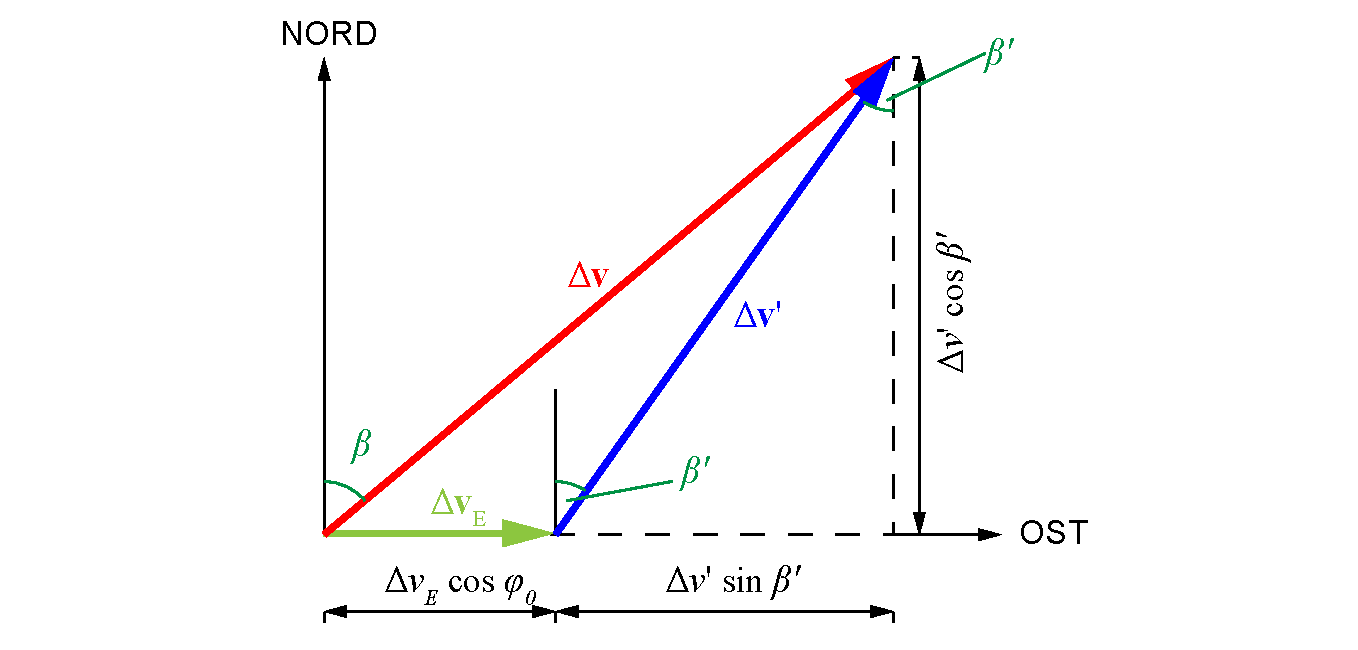
\includegraphics[width=\textwidth]{StartAzimutInertial.pdf} 
	\caption[Ber�cksichtigung der Erdrotation beim Start von Raketen.]{Ber�cksichtigung der Erdrotation beim Start von Raketen.}
	\label{abb:adyn_launch_lsg07}
\end{figure}

F�r die Berechnung der 3D-Trajektorien haben wir drei M�glichkeiten:
\begin{enumerate}[a)]
	\item Wir betrachten alles im geozentrisch-raumfesten Inertialsystem und l�sen numerisch die Bewegungsgleichung \eqref{eq:adyn_launch_vec} in 3 Dimensionen. Dabei m�ssen wir bei den Anfangsbedingungen die von der Rakete mitgenommene Rotation der Erde nach \eqref{eq:adyn_launch_lsg09} ber�cksichtigen, ebenso wie das umgerechnete Startazimut $\beta$ und den Anfangs-FPA $\gamma_0$ nach \eqref{eq:adyn_launch_lsg10} \bzw \eqref{eq:adyn_launch_lsg11}. Man beachte, dass die beiden Gr��en im topozentrischen System definiert sind und mit den Ortskoordinaten des Startorts in das Inertialsystem umgerechnet werden m�ssen.\\
	Bei der Berechnung der Reibung muss man ber�cksichtigen, dass die Atmosph�re mitrotiert und folglich die f�r die Reibung ma�gebliche aktuelle Geschwindigkeit $v'$ aus der im Inertialsystem geltenden Geschwindigkeit in $v$ umgerechnet werden muss:
\begin{align}
\begin{split}
		\vec{v}'(t) &= \vec{v}(t) - \vec{v}_\text{E,0} ~~~\text{mit}~~~\vec{v}_\text{E,0} = \vec\omega_\text{E} \times \vec{r}_0 \,.
\end{split} \label{eq:adyn_launch_lsg12}
\end{align}
Die Bewegungsgleichung lautet also:
\begin{align}
\begin{split}
		\vec{\ddot{r}}\begin{pmatrix} \ddot{x}\\ \ddot{y} \\ \ddot{z} \end{pmatrix} &=  \frac{\vec{F}_\text{S}(t) + \vec{F}_\text{G}(t) - \vec{F}_\text{D}(t)}{m_\text{R}(t)} = 
		\frac{F_\text{S}(t)}{m_\text{R}(t)\,v(t)} \begin{pmatrix} \dot{x}\\ \dot{y} \\ \dot{z} \end{pmatrix} 
 - \frac{G\,M_\text{E}}{\left| \vec{r}(t) \right|^3} \begin{pmatrix} x \\y\\z \end{pmatrix}
 - \frac{\varrho(r)\, v'\, A \,c_\text{D}}{m_\text{R}(t)} \begin{pmatrix} \dot{x}'\\ \dot{y}'\\ \dot{z}' \end{pmatrix}\,.
\end{split} \label{eq:adyn_launch_lsg13}
\end{align}
Die Nickkorrektur wird wie folgt berechnet:\\ 
Nach Bestimmung der Geschwindigkeit zum Zeitpunkt kurz vor der Nickkorrektur $\vec{v}(t=t_\text{Nick-})$, die sich ohne der mitgenommenen
Rotation der Erde ergibt (also nur die Geschwindigkeitszunahme durch den Schub), erfolgt 
die Drehung des Geschwindigkeitsvektors/Schubvektors um den Nickwinkel $\gamma_\text{N}$ in Richtung des Startazimuts. Diese Drehung wird im Horizontsystem 
mit folgender Drehmatrix $\mathbb{R}_\text{Nkorr}$ beschrieben, wobei hierbei zuerst die
Nickkorrektur und dann die Ausrichtung auf das Azimut ausgef�hrt wird. Die dazu notwendigen Berechnung der Drehmatritzen f�hren wir in einer Nebenrechnung aus:

\begin{nebenrechnungNeu} {Einheitsvektoren und Transformationsmatrix}

\begin{align*}
    \vec{r} &= r\,\begin{pmatrix} \sin\theta\,\cos\phi \\ \sin\theta\,\sin\phi \\ \cos\phi \end{pmatrix} ~~ \text{\bzw in geograph. Koord.}~~~ \vec{r} = r\,\begin{pmatrix} \cos\varphi\,\cos\lambda \\ \cos\varphi\,\sin\lambda \\ \sin\varphi \end{pmatrix}\\
    \vec{e}_\text{r} &= \frac{\d\vec{r}}{\d r} \;= \;\begin{pmatrix} \sin\theta \,\cos\phi \\ \sin\theta\,\sin\phi \\ \sin\phi \end{pmatrix}\; \widehat{=} \;\begin{pmatrix} \cos\varphi\,\cos\lambda \\ \cos\varphi\,\sin\lambda \\ \sin\varphi \end{pmatrix}\\
     \vec{e}_\theta &= \frac{1}{r}\,\frac{\d\vec{r}}{\d \theta}\;=\; \begin{pmatrix} \cos\theta \,\cos\phi \\ \cos\theta \,\sin\phi \\ -\sin\phi \end{pmatrix}\;\widehat{=}\;\vec{e}_\varphi = \frac{1}{r}\,\frac{\d\vec{r}}{\d \varphi}\;=\; \begin{pmatrix} -\sin\varphi \,\cos\lambda \\ -\sin\varphi\,\sin\lambda \\ \cos\varphi \end{pmatrix} \\
     \vec{e}_\phi &= \frac{1}{r\,\sin\theta}\,\frac{\d\vec{r}}{\d \phi}\;=\; \begin{pmatrix} -\sin\phi\\ \cos\phi \\ 0 \end{pmatrix}\;\widehat{=}\;\vec{e}_\lambda = \frac{1}{r\,\cos\varphi}\,\frac{\d\vec{r}}{\d \lambda}\;=\; \begin{pmatrix} -\sin\lambda \\ \cos\lambda\\ 0 \end{pmatrix} \\
    \rightarrow \mathbb{S} &= \lk \vec{e}_\text{r},\,\vec{e}_\theta,\,\vec{e}_\phi \rk \;=\; \begin{pmatrix} \cos\varphi\,\cos\lambda & -\sin\phi\,\cos\varphi & -\sin\lambda \\ \cos\varphi\,\sin\lambda & -\sin\varphi\,\cos\lambda & \cos\lambda \\ \sin\varphi & \cos\varphi& 0 \end{pmatrix}
\end{align*}

\end{nebenrechnungNeu}

Wir erhalten damit:

\begin{align}
\begin{split}
		\mathbb{R}_\text{Nkorr} &= \mathbb{R}_\text{A}\, \mathbb{R}_\text{N} ~~\text{mit}~~\\
		\mathbb{R}_\text{N} &= \begin{pmatrix} \cos\gamma_\text{N} & ~~-\sin\gamma_\text{N} & ~~0 \\
		                                      \sin\gamma_\text{N} & ~~+\cos\gamma_\text{N} & ~~0 \\
																					0 & 0 & 1\end{pmatrix}\ ~~\text{und}~~
		\mathbb{R}_\text{A} = \begin{pmatrix} 1 &~~ 0 &~~ 0 \\
		                                      0 &~~\cos\beta' & ~~-\sin\beta'\\
		                                      0 &~~\sin\beta' & ~~+\cos\beta' \end{pmatrix}\,.
\end{split} \label{eq:adyn_launch_lsg14}
\end{align}
Die so berechnete Drehmatrix geht jedoch davon aus, dass die Rakete vor der
Nickkorrektur entlang der $x$-Richtung der Drehmatrix ausgerichtet ist. In unserem Fall ist die Rakete aber radial nach au�en gerichtet. Daher muss die Drehmatrix noch
in das richtige (sph�rische) Koordinatensystem transformiert werden. (Siehe auch \mscr~\mladynref{KOS.m}):
\begin{align}
\begin{split}
  \mathbb{R}_\text{Nkorr}' &= \mathbb{S} \,\mathbb{R}_\text{Nkorr}\, \mathbb{S}^\text{T}~~~\text{mit}~~~\\
	\mathbb{S} &= \begin{pmatrix} \vec{e}_r  & \vec{e}_\varphi &\vec{e}_\lambda \end{pmatrix} =
	              \begin{pmatrix} \cos\varphi\,\cos\lambda &~~ -\sin\varphi\,\cos\lambda &~~ -\sin\lambda\\
			                          \cos\varphi\,\sin\lambda &~~ -\sin\varphi\,\sin\lambda &~~ +\cos\lambda\\
			                          \sin\varphi)                &~~ +\cos\varphi                &~~ 0 \end{pmatrix}\,.
\end{split} \label{eq:adyn_launch_lsg15}
\end{align}
Der Geschwindigkeitsvektor (zugleich die Schubrichtung) der Rakete nach Nickkorrektur ist dann:
\begin{align*}
\vec{v}(t=t_\text{Nick+})  = \mathbb{R}_\text{Nkorr}'\,\vec{v}(t=t_\text{Nick-})\,.
\end{align*}
Wir bestimmen die H�he, den FPA, die Geschwindigkeit und die Masse der Rakete f�r die einzelnen Stufen bis die Rakete einen FPA von 0 hat. Dann erfolgt nur noch ein tangentialer Schub bis zum Erreichen der notwendigen Kreisbahngeschwindigkeit. 

Das Ergebnis der Rechnungen ist in \figref{adyn_launch_lsg08} und \figref{adyn_launch_lsg09} dargestellt und im \mscr~\mladynref{Raketenstart2Orbit04.m} ausgef�hrt und ausf�hrlich erl�utert.

\begin{figure}[H]
	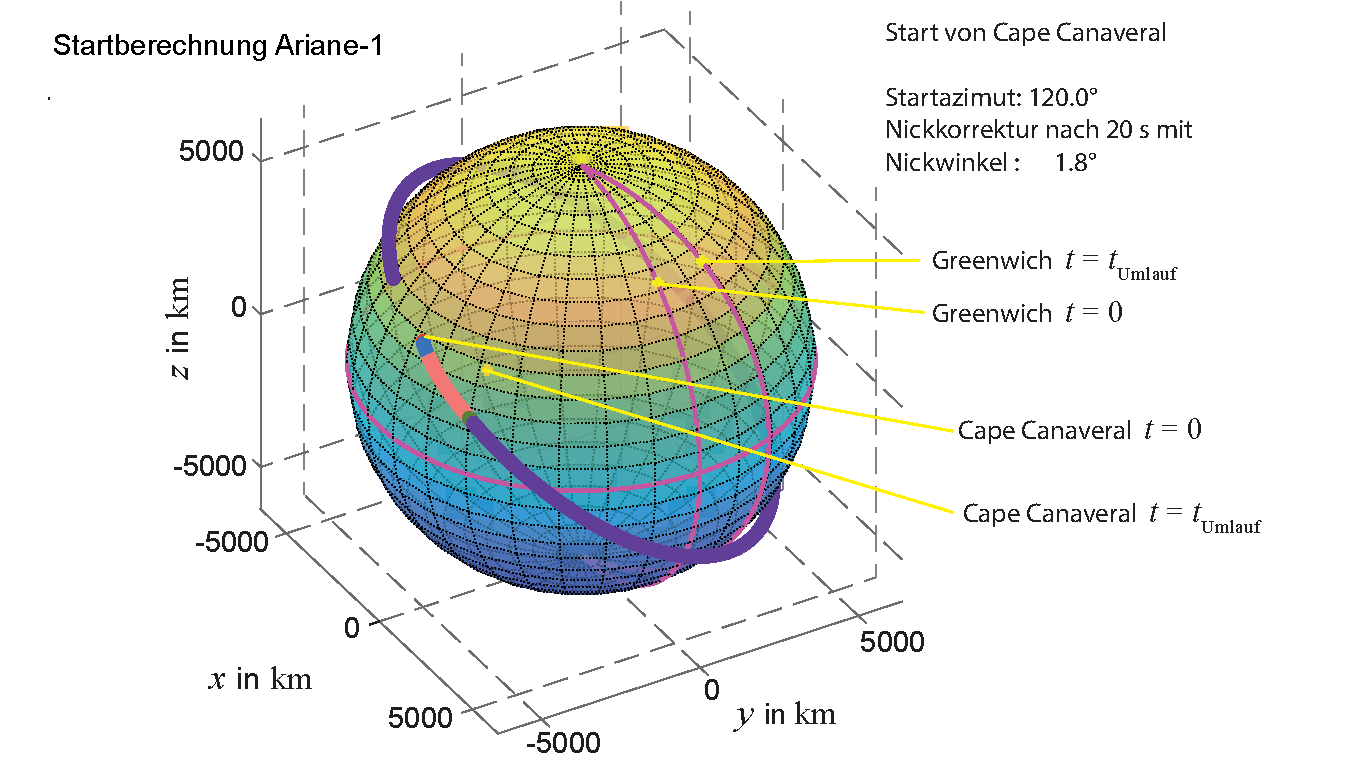
\includegraphics[width=\textwidth]{StartAriane01.pdf} 
	\caption[Trajektorie nach Start von der Erdoberfl�che.]{Trajektorie nach Start von der Erdoberfl�che. Parameter siehe \mladynref{Raketenstart2Orbit04.m}.}
	\label{abb:adyn_launch_lsg08}
\end{figure}

\begin{figure}[H]
	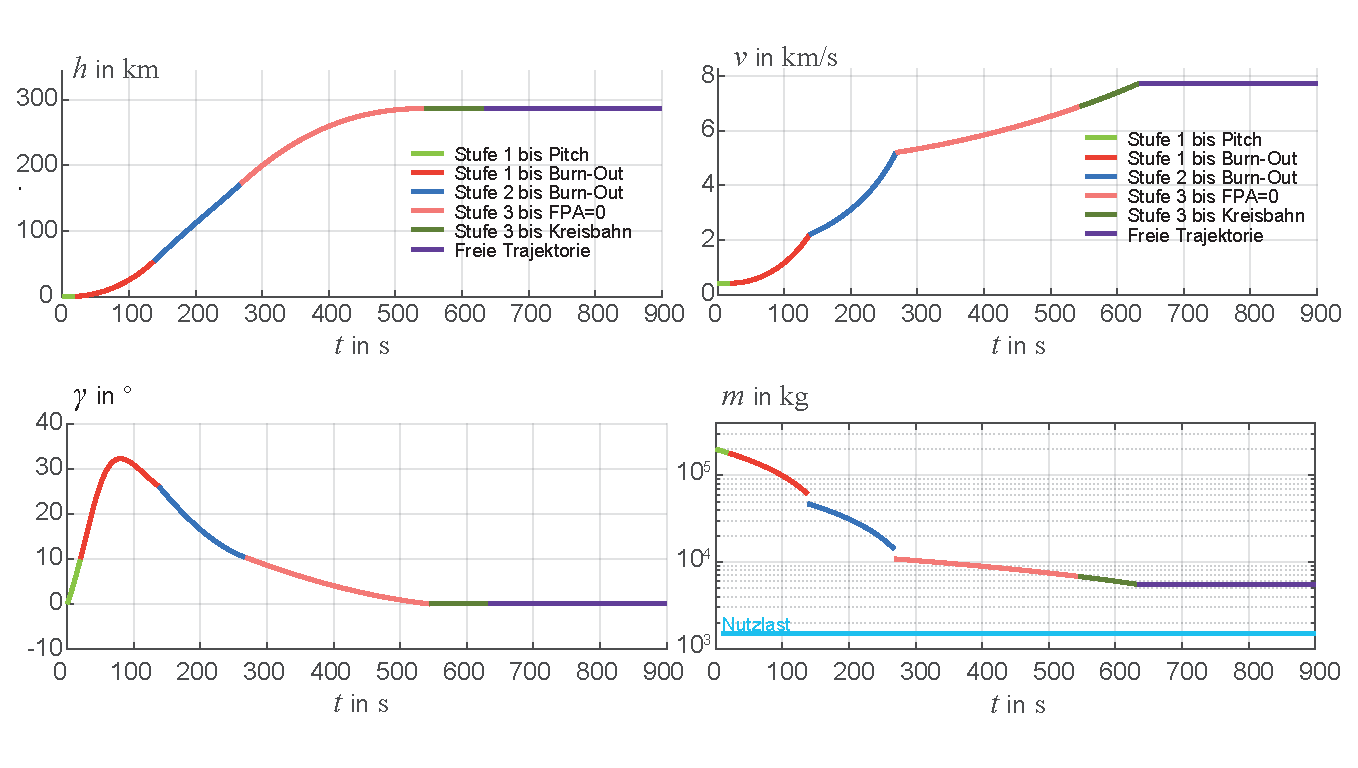
\includegraphics[width=\textwidth]{StartAriane02.pdf} 
	\caption[H�he, FPA,  Geschwindigkeit und  Masse der Ariane 1 nach Start von der Erdoberfl�che.]{H�he, FPA,  Geschwindigkeit und  Masse der Ariane 1 nach Start von der Erdoberfl�che. Parameter siehe \mladynref{Raketenstart2Orbit04.m}.}
	\label{abb:adyn_launch_lsg09}
\end{figure}

\item Als Alternative kann man die Trajektorien nat�rlich auch im mitbewegten \KOS des Beobachters im Horizontsystem berechnen. Das f�hrt auf �hnliche Rechnungen wie wir im Kap. 1.3.2 im Band I (Physik Bewegung) zum Wurf und freien Fall auf der Erdoberfl�che gemacht hatten.
\item Als weitere Alternative k�nnen wir nat�rlich das Ergebnis der Rechnungen im mitbewegten \KOS (Siehe Teilaufgabe 2) benutzen und ins Inertialsystem transformieren. Zwei Ortsvektoren sind dabei ausgezeichnet: Der Vektor zum Startpunkt und der Vektor zum aufsteigenden Knoten. Die Inklination und der aufsteigende Knoten der Bahn sind durch Startazimut, Startfenster und geographische Position des Startortes gegeben. Die Transformation erfolgt �ber die im \kap{hm_bahnen_hk_PQR} hergeleiteten Matrizen.\\
Wir empfehlen dem Leser zur Vervollst�ndigung des Bildes beide Alternativen selbst zu rechnen.
\end{enumerate}

\end{subprobs}
\end{sol} 
\textcolor{blue} {$\rightarrow$ zur} \probref{adyn_launch01}.\\
\noindent\rule[1ex]{\textwidth}{0.5pt}  \newpage  \clearpage

%-----------------------------------------------------------------------------------------------------------

\begin{sol}{prob:adyn_reentry01}\label{lsg:adyn_reentry01} %�bung27
\textbf{Parameter des Wiedereintritts in die Erdatmosph�re}\\

\begin{figure}[H]
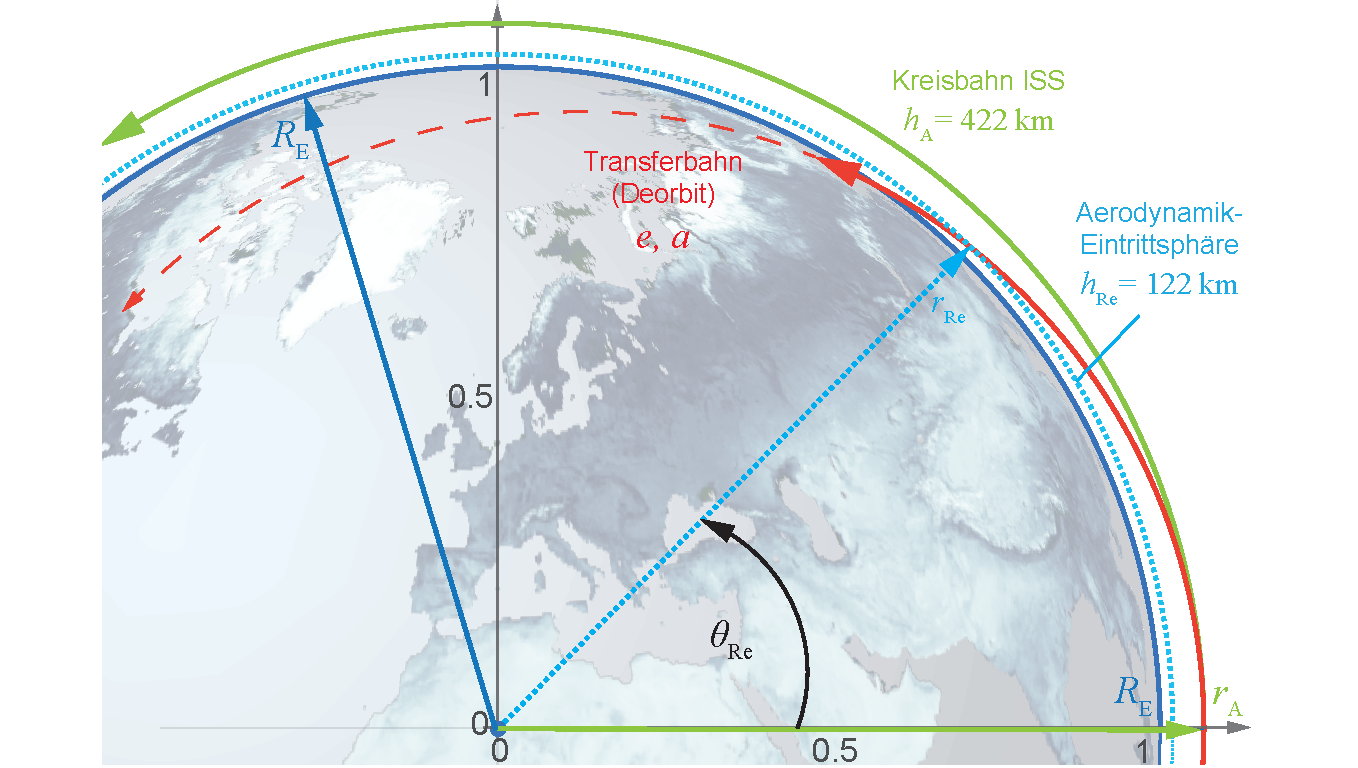
\includegraphics[width=\textwidth]{ReentryGeometrie01.pdf}
\caption[Geometrie des Wiedereintritts in die Erdatmosph�re.]{Geometrie des Wiedereintritts in die Erdatmosph�re. Siehe auch \mscr~\mladynref{Transfer2Reentry.m} f�r weitere Details und Graphiken.}
\label{abb:adyn_reentry_geometrie01}
\end{figure}

\begin{figure}[H]
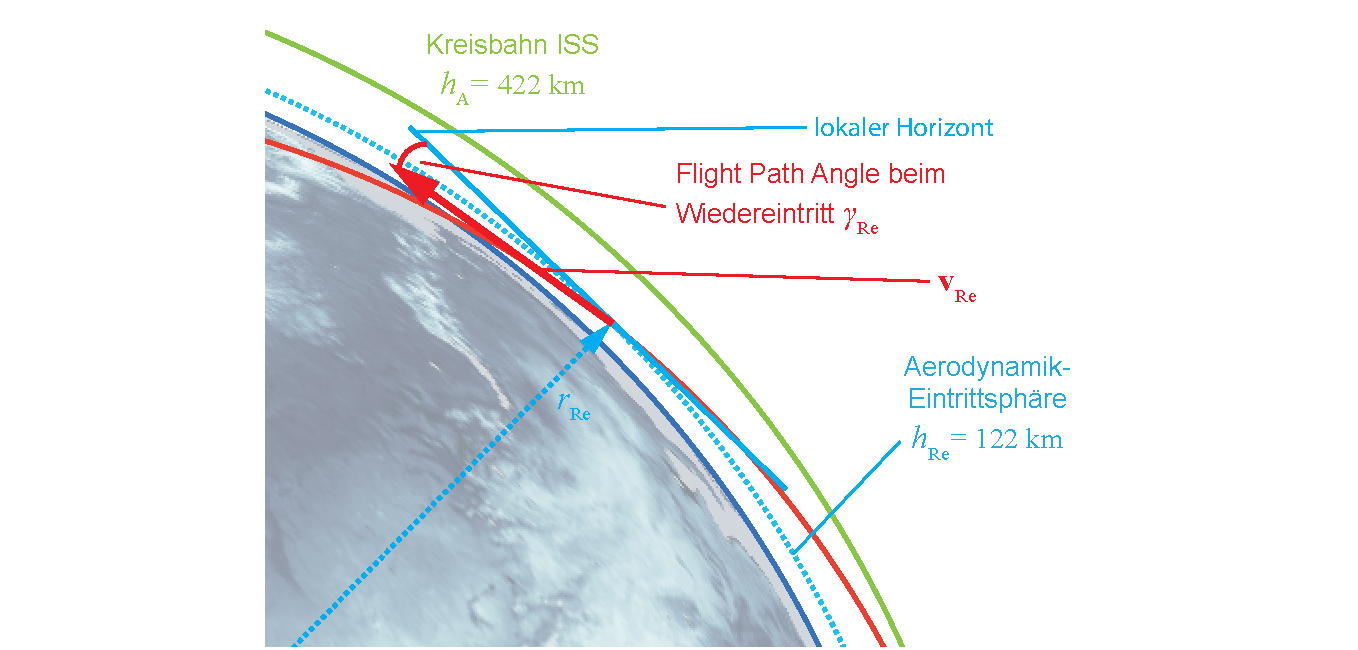
\includegraphics[width=\textwidth]{ReentryGeometrie02.pdf}
\caption[Geometrie des Wiedereintritts in die Erdatmosph�re.]{Geometrie  (Detail) des Wiedereintritts in die Erdatmosph�re. Siehe auch \mscr~\mladynref{Transfer2Reentry.m} f�r weitere Details und Graphiken.}
\label{abb:adyn_reentry_geometrie02}
\end{figure}

%\begin{nebenrechnung}
%\begin{align*}
    %e &= \frac{q^2-\lk 2q-1\rk\,\cos^2\gamma_\text{Re}}{q^2-\cos^2\gamma_\text{Re}} = \frac{q^2-\lk 2q-1\rk\,u^2}{q^2-u^2} \\
    %\cos\theta_\text{Re} &= q\,\frac{\lk 1-e\rk}{e}-\frac{1}{e} = \frac{q-1}{e}-q = \frac{Z}{N}\\
    %&= \frac{\lk q-1\rk\lk q^2-u^2\rk-q\,\lk q^2-\lk 2q-1\rk\,u^2\rk}{q^2-\lk2q-1\rk\,u^2}\\
    %N &= q^2-2\,q\,u^2+ u^2 = q^2-2q+1+2q-1-2\,q\,u^2+u^2\\
    %&= \lk q-1\rk^2 +\lk 2q-1\rk - \lk 2q-1\rk\,u^2 \\
    %&= \lk q-1\rk^2 + \lk2q-1\rk\lk1-u^2\rk \\
    %&= \hat{q}^2 + \lk 2q-1\rk\,\sin^2\gamma_\text{Re}\\
    %Z &=  \cancel{q^3} - \cancel{q\,u^2}-q^2+u^-\cancel{q^3} +2\,q^2\,u^2-\cancel{q\,u^2} = 2\,q^2\,u^2- 2\,q\,u^2 - q^2+u^2 \\
    %&= \lk q^2-2q+1\rk\,u^2 - \lk q^2-q^2\,u^2\rk = \hat{q}^2\,u^-q^2\,\lk1-u^2\rk\\
    %&= \hat{q}^2\,\cos^2\gamma_\text{Re} - q^2\,\sin^2\gamma_\text{Re}
%\end{align*}
%\end{nebenrechnung}

Wir haben die Geometrie des Deorbits in \figref{adyn_reentry_geometrie01} und \figref{adyn_reentry_geometrie02} dargestellt.\\
Gegeben sind $v_\text{A}$, $r_\text{A}$, $r_\text{Re}$ und der gew�nschte FPA $\gamma_\text{Re}$, gesucht sind der \anf{Ort} $\upsilon_\text{Re}$ \bzw $\theta_\text{Re}$ des \anf{Eintauchens} in die aerodynamische Zone/Sph�re und die Geschwindigkeit $v_\text{Re}$, die das Raumschiff dort hat. Dazu muss man die Bahnparameter $e$ \bzw $a$ kennen, f�r die gilt: $r_\text{A} = a\,\lk 1+e\rk$.\\
Wir starten mit Ellipsengleichung \eqref{eq:hm_kegelschnitt}:
\begin{align}
    r_\text{Re} = \frac{a\,\lk 1-e^2\rk}{1+e\,\cos\upsilon_\text{Re}} = \frac{a\,\lk1-e^2\rk}{1-e\,\cos\theta_\text{Re}} \,. \label{eq:adyn_lsg_reentry01}
\end{align}
Aus der vis-visa-Gleichung \eqref{eq:hm_vis-viva}, die wir zun�chst vektoriell aufschreiben aufschreiben, k�nnen wir eine Beziehung f�r $v_\text{Re}\lk r_\text{Re},\upsilon_\text{Re}\rk$ ableiten.
\begin{nebenrechnungNeu} {  }

\begin{align*}
   \text{Aus} ~~ \vec{L} \times\,\lk \vec{v}\times \vec{L}\rk &= \vec{v} \,\lk \vec{L}\vec{L}\rk - 			   \underbrace{\vec{L}\,\lk \vec{L}\vec{v}\rk}_{\substack{=0}} = L^2\,\vec{v} ~~
   \text{und}\\
    \vec{e} &= -\frac{1}{\mu}\,\lk \vec{L}\times \vec{v}\rk\,\frac{\vec{r}}{r}\,,~~~~
    \vec{v} = \frac{\mu}{L^2}\,\vec{L}\times\lk\vec{e} + \frac{\vec{r}}{r}\rk~~\text{folgt}\\
    \vec{L}\times \vec{v} &= -\mu\,\lk\frac{\vec{r}}{r}+\vec{e}\rk ~~\rightarrow~~
    \vec{L}\times\lk\vec{v}\times \vec{L}\rk = \vec{L}\times\mu\,\lk\frac{\vec{r}}{r} + \vec{e}\rk\,, \\
    L^2\,\vec{v} &= \mu\,\lek\vec{L}\times \lk\vec{e} + \frac{\vec{r}}{r}\rk\rek ~~\rightarrow~~~
    \vec{v} = \frac{\mu}{L^2}\lek \vec{L}\times\lk \vec{e}+ \frac{\vec{r}}{r}\rk\rek\,, \\
    \rightarrow~~~|\vec{v}| &=\frac{\mu}{L^2}\,\sqrt{\lek \vec{L}\times\lk \vec{e}+\frac{\vec{r}}{r}\rk\rek\lek\vec{L}\times\lk \vec{e}+\frac{\vec{r}}{r}\rk\rek}\,.\\
\text{Wegen}~~&\lk \vec{a}\times \vec{b}\rk\lk \vec{a}\times\vec{b}\rk = a^2\,b^2 -\lk a\,b\rk^2~~\text{folgt:}\\
    |\vec{v}| &= \frac{\mu}{L^2}\,\sqrt{L^2\,\lk \vec{e} + \frac{\vec{r}}{r}\rk^2 - \underbrace{\lek \vec{L}\,\lk \vec{e} + \frac{\vec{r}}{r}\rk\rek^2 }_{=0}}~~~\text{und da}~~~\vec{L} \perp \vec{e},\vec{r} \\
    |\vec{v}| &= \frac{\mu}{L^2}\,L\,\sqrt{\lk \vec{e} + \frac{\vec{r}}{r}\rk^2} = \frac{\mu}{L}\,\sqrt{e^2+2e\,\cos\upsilon_\text{e} +1}
\end{align*}
\end{nebenrechnungNeu}

Damit haben wir als zweite Gleichung:
\begin{align}
    v_\text{e} = \frac{\mu}{L}\,\sqrt{1+e\,\cos\upsilon_\text{Re} + e^2}\,. \label{eq:adyn_lsg_reentry02}
\end{align}
Als dritte Gleichung brauchen wir noch den FPA. Dieser ist gegeben durch den Winkel zwischen Geschwindigkeitsvektor $\vec{v}$ und lokalem Horizont.
Letzterer liegt senkrecht zum Radiusvektor (Abstandsvektor) $\vec{r}$ in der $\vec{r}$\,-\,$\vec{v}$-Bahnebene und stimmt mit der Richtung des Vektors $\vec{e}$ �berein.
Wir bilden das Skalarprodukt:
\begin{subequations}
\begin{align}
    \vec{v}\,\lk \frac{\vec{L}}{L}\times\frac{\vec{r}}{r}\rk &= r\,\dot{\upsilon} =v\,\cos\gamma\,, \label{eq:adyn_lsg_reentry03a}\\
    \vec{v}\,\frac{\vec{r}}{r} &= \dot{r} = \sin\gamma\,. \label{eq:adyn_lsg_reentry03b}
\end{align} \label{eq:adyn_lsg_reentry03}
\end{subequations}
Aus \eqref{eq:adyn_lsg_reentry03a} folgt mit \eqref{eq:adyn_lsg_reentry02} und $L = r^2\,\dot{\upsilon}$:
\begin{subequations}
\begin{align}
    \cos\gamma_\text{Re} = \frac{1+e\,\cos\upsilon_\text{Re}}{\sqrt{1+2e\,\cos\upsilon_\text{Re} + e^2}}\,,\label{eq:adyn_lsg_reentry04a} \\
    \sin\gamma_\text{Re} = \frac{e\,\sin\upsilon_\text{Re}}{\sqrt{1+2e\,\cos\upsilon_\text{Re}+e^2}}\,. \label{eq:adyn_lsg_reentry04b}
\end{align} 
\end{subequations}
Man kann folglich mit \eqref{eq:adyn_lsg_reentry04a} und  \eqref{eq:adyn_lsg_reentry04b} auch die Geschwindigkeit an einem beliebigen Bahnpunkt durch
\begin{align}
\begin{split}
    \vec{v} &= \frac{\mu}{L}
    \begin{pmatrix}
        \sin\gamma \\
        \cos\gamma
    \end{pmatrix}
    =
    \frac{\mu}{L}
    \begin{pmatrix}
        e\,\sin\upsilon \\
        1+e\,\cos\upsilon
    \end{pmatrix} \\
    &= \sqrt{\frac{\mu^{\killA{2}}}{\killA{\mu}\,a\,\lk 1-e^2 \rk}}
    \begin{pmatrix}
        e\,\sin\upsilon \\
        1+e\,\cos\upsilon
    \end{pmatrix} 
    =\sqrt{\frac{\mu}{p}}
     \begin{pmatrix}
        e\,\sin\upsilon \\
        1+e\,\cos\upsilon
    \end{pmatrix} 		
\end{split} \label{eq:adyn_lsg_reentry05}
\end{align}
in der Koordinate $\upsilon$ und den Bahnparametern $p$, $e$ ausdr�cken. \\
Zus�tzlich zu Gleichungen \eqref{eq:adyn_lsg_reentry01}, \eqref{eq:adyn_lsg_reentry02} und \eqref{eq:adyn_lsg_reentry04a} gilt noch $r_\text{A} = a\,\lk1+e\rk$ und $q= r_\text{A}/r_\text{Re} > 1$.
Aus \eqref{eq:adyn_lsg_reentry01} k�nnen wir dann folgende Beziehung ableiten:
\begin{align}
   e\,\cos\upsilon_\text{Re} &= \frac{a\,\lk 1-e^2\rk}{r_\text{Re}} -1 = \frac{a\,\lk 1+e\rk\lk 1-e\rk}{r_\text{Re}} = q\,\lk 1-e\rk-1 \,. \label{eq:adyn_lsg_reentry05a} 
\end{align}
Wir benutzen \eqref{eq:adyn_lsg_reentry05a} in \eqref{eq:adyn_lsg_reentry01} und erhalten:
\begin{align}
\begin{split}
    \cos\gamma_\text{Re} &= \frac{q\,\lk 1-e\rk}{\sqrt{1+2q\,\lk 1-e\rk -2+e^2}}
    = q\,\sqrt{\frac{\lk 1-e\rk^2}{2q-2\,e\,q-1+e^2}}\\
    &= q\,\sqrt{\frac{\lk 1-e\rk^2}{2q-2\,e\,q-\lk 1-e^2\rk}}
    = q\,\sqrt{\frac{\lk 1-e\rk^2}{2q\,\lk 1-e\rk - \lk 1+e\rk\lk1-e\rk}}
    = q\,\sqrt{\frac{1-e}{2q-\lk 1+e\rk}}
\end{split} \label{eq:adyn_lsg_reentry06} 
\end{align}
F�r $v_\text{Re}$ erhalten wir:
\begin{align}
\begin{split}
    v_\text{Re} &= \frac{\mu}{L}\,\sqrt{1+2e\,\cos\upsilon_\text{Re} +e} = \sqrt{\frac{\mu\,\lk 1+2q\,\lk 1-e\rk -1+e^2\rk}{r_\text{A}\,\lk 1-e^2\rk}}\\
    &= \sqrt{\frac{\mu}{r_\text{A}}}\,\sqrt{\frac{2q-2\,q\,e-1+e^2}{\lk 1+e\rk\lk 1-e\rk}} = \sqrt{\frac{\mu}{r_\text{A}}}\,\,\sqrt{\frac{2q\,\cancel{\lk 1-e\rk}}{\lk 1+e\rk\cancel{\lk 1-e\rk}} - \cancel{\frac{\lk 1-e^2\rk}{\lk 1+e\rk\lk1-e\rk}}} \\
    &= \sqrt{\frac{\mu}{r_\text{A}}}\,\sqrt{\frac{2q-\lk 1+e \rk}{\lk 1+e\rk}} = \sqrt{\frac{\mu}{r_\text{A}\,\lk 1+e\rk}}\,\sqrt{2q-\lk 1+e\rk}
\end{split}\label{eq:adyn_lsg_reentry07}
\end{align}
Aus \eqref{eq:adyn_lsg_reentry06} k�nnen wir die Exzentrizit�t $e$ bestimmen und dann $v_\text{Re}$ �ber \eqref{eq:adyn_lsg_reentry07}. 
\begin{align*}
\begin{split}
    \frac{u^2}{q^2} &= \frac{1-e}{2q-\lk 1+e\rk} ~~~~\text{mit}~~~~ u = \cos\gamma_\text{Re}\\ 
		u^2\,\lek 2q-\lk 1+e\rk\rek &= \lk 1-e\rk ~~\rightarrow~~
    \frac{u^2}{q^2}\,2q -\frac{u^2}{q^2}\,\lk 1\rk - \frac{u^2}{q^2}\,e^2 = 1-e \,,\\
    %\rightarrow~~\frac{u^2}{q^2}\,\lk 2q-1\rk -1 &= \frac{u^2}{q^2}\,e-1 = e\lk \frac{u^2}{q^2}-1\rk\\
    \rightarrow~~ e &= \frac{\lek \frac{u^2}{q^2}-\lk 2q-1\rk -1\rek}{\lek \frac{u^2}{q^2} -1\rek} = \frac{u^2\,\lk 2q-1\rk-q^2}{u^2-q^2} \\
    &= \frac{q^2-\cos^2\gamma_\text{Re}\,\lk 2q-1\rk}{q^2-\cos^2\gamma_\text{Re}}\,.
\end{split} 
\end{align*}
Mit der Beziehung f�r $e$, die man in \eqref{eq:adyn_lsg_reentry07} einsetzt, erh�lt man die Beziehungen \eqref{eq:adyn_reentry03} f�r $v_\text{Re}$ \bzw $\vec{v}_\text{Re}$ und �ber $\Delta \vec{v} = \vec{v}_\text{Re} - \vec{v}_\text{A}$, auch $|\Delta \vec{v}| =\Delta v$.

Wir vergleichen zum Schluss noch die Problemstellungen des Lambert-Transfers und des Wiedereintritt-Transfers miteinander:
\begin{table}[ht]
		\begin{center}
    \begin{tabular}{|L{2.5cm}|L{5cm}|}
    \hline
    \rule{0pt}{3pt}&  \\
    \rule{0pt}{6pt}\textit{Lambert-Problem} &  \\
 %   \rule{0pt}{3pt} &   \\
      Gegeben: & $r_1,\, r_2,\, \gamma = \angle (r_1,r_2),\, \Delta t$ \\
			Gesucht: & $a,\, e$,\, $v_\text{1,tr},\, \Delta v$ \\
    \rule{0pt}{3pt}&  \\
    \rule{0pt}{6pt}\textit{Deorbit-Transfer}& \\
%    \rule{0pt}{3pt}&  \\
      Gegegen: & $r_1, r_2,\, \text{FPA} =\gamma_\text{Re},\, v_\text{A}$ \\
			Gesucht: & $e,\, \upsilon_\text{Re} $,\, $v_\text{Re},\, \Delta v$ \\
    \rule{0pt}{3pt}&  \\
    \hline
    \end{tabular} 
		\end{center}
		\caption{Vergleich Lambert-Problem und Parameterbestimmung Reentry}
		\label{tab:adyn_vglLambertReentry}
\end{table}


\end{sol} 
\textcolor{blue} {$\rightarrow$ zur} \probref{adyn_reentry01}.\\
\noindent\rule[1ex]{\textwidth}{0.5pt}  \newpage  \clearpage

%-----------------------------------------------------------------------------------------------------------

\begin{sol}{prob:adyn_reentry02}\label{lsg:adyn_reentry02} %�bung28
\textbf{Auftrieb/Drag-Abh�ngigkeit bei Wiedereintritt in Erdatmosph�re}\\

Die Rechnung sind im \mscr~\mladynref{ReentryReal.m} im Detail hinterlegt.

\begin{figure}[H]
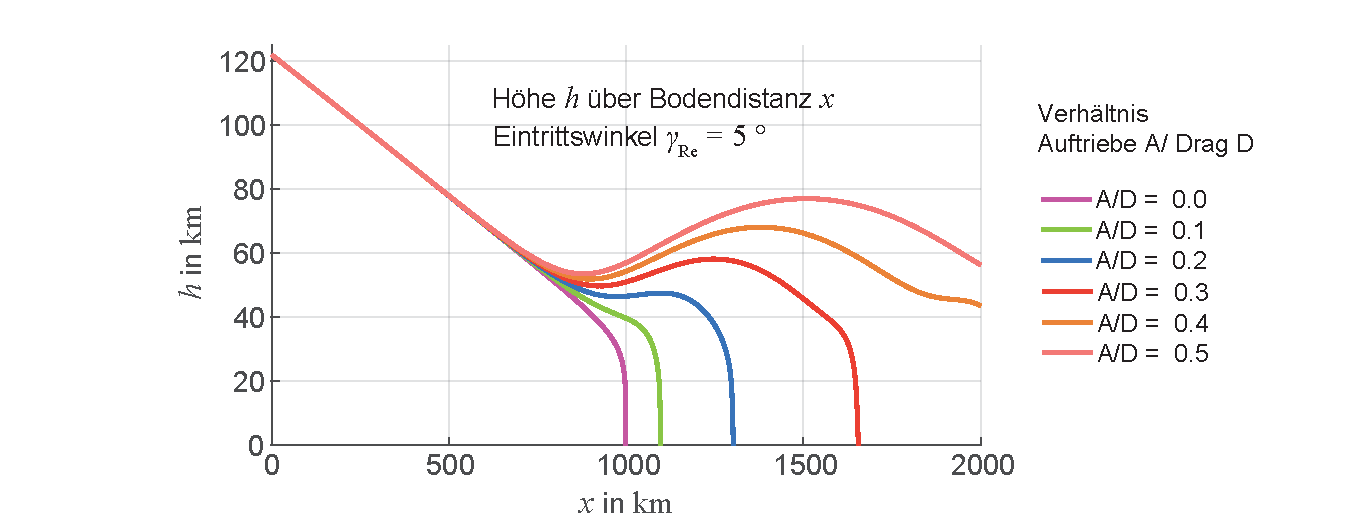
\includegraphics[width=\textwidth]{Reentry_Uebung01.pdf}
\caption[H�he $h$ nach Wiedereintritt in die Erdatmosph�re �ber die Bodendistanz $x$.]{H�he $h$ nach Wiedereintritt in die Erdatmosph�re �ber die Bodendistanz $x$ in Abh�ngigkeit vom Auftrieb/Drag-Verh�ltnis. Siehe \mscr~\mladynref{ReentryReal.m} f�r Parameter und Details.}
\label{abb:adyn_reentry_uebung01}
\end{figure}

\begin{figure}[H]
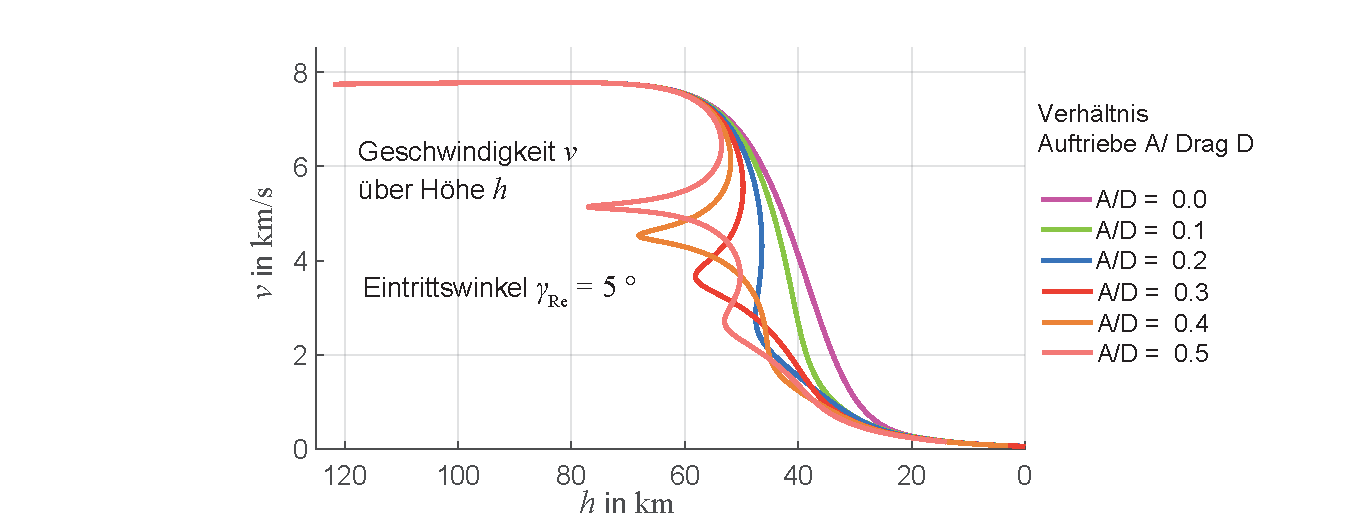
\includegraphics[width=\textwidth]{Reentry_Uebung02.pdf}
\caption[Geschwindigkeit $v$ nach Wiedereintritt in die Erdatmosph�re �ber die H�he $h$.]{Geschwindigkeit $v$ nach Wiedereintritt in die Erdatmosph�re �ber die H�he $h$ in Abh�ngigkeit vom Auftrieb/Drag-Verh�ltnis. Siehe \mscr~\mladynref{ReentryReal.m} f�r Parameter und Details.}
\label{abb:adyn_reentry_uebung02}
\end{figure}

\begin{figure}[H]
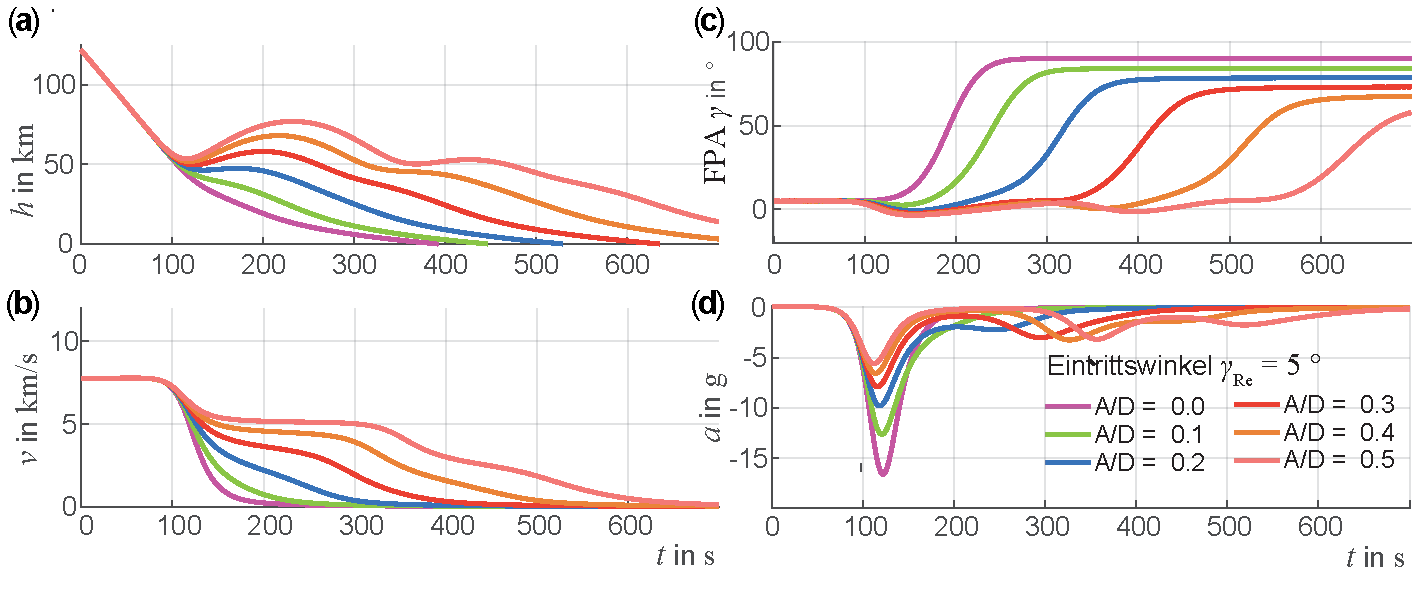
\includegraphics[width=\textwidth]{Reentry_Uebung03.pdf}
\caption[Verschieden Parameter nach Wiedereintritt als Funktion der Zeit.]{H�he $h$ \fa, Geschwindigkeit $v$ \fb, Flight Path Angle FPA \fc und Beschleunigung $a$ \fd nach Wiedereintritt in die Erdatmosph�re �ber die Zeit $t$ in Abh�ngigkeit vom Auftrieb/Drag-Verh�ltnis. Siehe \mscr~\mladynref{ReentryReal.m} f�r Parameter und Details.}
\label{abb:adyn_reentry_uebung03}
\end{figure}

\end{sol} 
\textcolor{blue} {$\rightarrow$ zur} \probref{adyn_reentry02}.\\
\noindent\rule[1ex]{\textwidth}{0.5pt}  \newpage  \clearpage

%-----------------------------------------------------------------------------------------------------------

\begin{sol}{prob:adyn_reentry03}\label{lsg:adyn_reentry03} %�bung29
\textbf{Normierte Gleichungen f�r $v(h)$ und $\gamma(h)$ bei Wiedereintritt}\\

F�r den Fall $F_\text{S}=0$ (was \zb f�r das Space Shuttle oft nicht erf�llt ist!) starten wir von:
\begin{subequations}
    \begin{align}
        \dot{v} &= -\frac{F_\text{D}}{m_\text{R}} - g\lk h\rk\,\sin\gamma = -v^2\,\frac{K_\text{D}}{H_0}\,\e^{-\frac{h}{H_0}}-g\,\sin \gamma\,,\\
        v\,\dot{\gamma} &= -\frac{F_\text{A}}{m_\text{R}} + \lk g\lk h\rk  - \frac{v^2}{r}\rk\,\cos\gamma\,,\\
        \dot{h} &= -v\,\sin\gamma\,,\\
        \dot{x} &= v\,\cos\gamma\,. 
    \end{align} \label{eq:adyn_normierte01}
\end{subequations}

Wir benutzen die barometrische H�henformel, sowie folgende Beziehungen f�r dem Drag und den Auftrieb:
\begin{subequations}
    \begin{align}
        F_\text{D} &= \frac{1}{2}\,\varrho\lk h\rk \,v^2\,C_\text{D}\,A_\text{R} = m_\text{R}\,v^2\,\frac{\kappa_\text{D}}{H_0}\,\e^{-\frac{h}{H_0}}\,,\\
        F_\text{A} &= \frac{1}{2}\,\varrho\lk h\rk \,v^2\,C_\text{A}\,A_\text{R} = m_\text{R}\,v^2\,\frac{\kappa_\text{A}}{H_0}\,\e^{-\frac{h}{H_0}}\,.
    \end{align} \label{eq:adyn_normierte02}
\end{subequations}

F�r $g\lk h\rk$ setzen wir an:
\begin{align}
    g\lk h\rk = g_0\,\frac{R_\text{E}{}^2}{r^2} = g_0\,\frac{R_\text{E}{}^2}{\lk R_\text{E}+h\rk^2}\,.  \label{eq:adyn_normierte03}
\end{align}
Wir normalisieren nun das DGL-System mit:
\begin{align}
    \begin{split}
        \mu &= \frac{v}{v_\text{K}} = \frac{v}{\sqrt{g_0\,R_\text{E}}} = \frac{v}{\sqrt{G\,M_\text{E}}}\\
        \eta &= \frac{h}{H_0}\,, ~~~~~~~~ \tau = \frac{g_0}{v_\text{K}}\,t\,, ~~~~~~~~
        \chi= \frac{x}{H_0}\, \\
        \D\tau &= \frac{g_0}{v_\text{K}}\,\D t\,, ~~~~~~~~ \D t = \frac{v_\text{K}}{g_0}\,\D \tau
    \end{split}\label{eq:adyn_normierte04}
\end{align}
und erhalten:
\begin{subequations}
    \begin{align}
        \begin{split}
            \frac{\D}{\D t}\,v &= -v^2\,\frac{\kappa_\text{D}}{H_0}\,\e^{-\frac{h}{H_0}} +g_0\,\frac{R_\text{E}{}^2}{r^2}\,\sin\gamma ~~~
            \rightarrow ~~~ \frac{\D}{\D \tau}\,\mu = -\mu^2\,\kappa_\text{D}\,\frac{R_\text{E}}{H_0}\,\e^{-\eta} +\sin\gamma\,.
          \end{split}
          \label{eq:adyn_normierte05a}
    \end{align}
und
    \begin{align}
        \begin{split}
            v\,\frac{\D}{\D t}\,\gamma &= -v^2\,\frac{\kappa_\text{A}}{H_0}\,\e^{-\frac{h}{H_0}} +\lk g-\frac{v^2}{r}\rk\,\cos\gamma~~~
            \rightarrow ~~~~ \mu\,\frac{\D}{\D\tau}\,\gamma =  -\mu^2\,\kappa_\text{D}\,\frac{A}{D}\,\frac{R_\text{E}}{H_0}\,\e^{-\eta} +\lk 1-\mu^2\rk\,\cos\gamma\,. 
          \end{split}
          \label{eq:adyn_normierte05b}
    \end{align}\label{eq:adyn_normierte05}
\end{subequations}
Die Gleichungen f�r H�he und Bodendistanz werden einfach zu:
\begin{subequations}
    \begin{align}
      \frac{\D}{\D\tau}\,\eta
      & = -\frac{R_\text{E}}{H_0}\, \mu\,\sin\gamma\,,
        \label{eq:adyn_normierte06a}\\
      \frac{\D}{\D\tau}\,\chi
      & = +\frac{R_\text{E}}{H_0}\,\mu\,\cos\gamma\,. \label{eq:adyn_normierte06b}
    \end{align} 
\end{subequations}

Wir setzen jetzt $\hat{\epsilon} = \mu^2$ und $\hat{\eta} = 2\,\frac{\kappa_\text{D}}{\sin\gamma_\text{Re}}\,\e^{-\eta}$ in \eqref{eq:adyn_normierte05} ein und erhalten mit der Substitution $\D \tau \rightarrow \D \hat{\eta} $ (siehe Nebenrechnung):
\begin{subequations}
  \begin{align}
    \frac{\D\lk \ln \hat{\epsilon}\rk}{\D \hat{\eta}}
    &= - \frac{\sin\gamma_\text{Re}}{\sin\gamma}
      + \frac{2H_0}{\hat{\epsilon}\,\hat{\eta}\,R_\text{E}}\,,
      \label{eq:adyn_normierte07a}\\
    \frac{\D\lk \cos\gamma\rk}{\D \hat{\eta}}
    &= \frac{\sin\gamma_\text{Re}}{2}\,\frac{A}{D}
      - \lk \frac{1}{\hat{\epsilon}}-1 \rk \,\frac{H_0\,\cos\gamma}
      {\hat{\eta}\,R_\text{E}}\,.
      \label{eq:adyn_normierte07b}
  \end{align}\label{eq:adyn_normierte07}
\end{subequations}

Die erste Gleichung ist eine Gleichung f�r die Entwicklung der (dimensionslosen) Energie $\hat{\epsilon}$ als Funktion der (dimensionslosen) H�he $\hat{\eta}$ und die zweite eine des FPA $\gamma$ ebenfalls als Funktion der H�he.

\begin{nebenrechnungNeu}  {  }

  Zun�chst nehmen wir uns \eqref{eq:adyn_normierte07a} vor.
  Wir beginnen mit der Ableitung und ber�cksichtigen die eingef�hrten
  Koordinatentransformationen, die eine mehrfache Verkettung enthalten,
  \begin{equation}
    \frac{\D\lk \ln \hat{\epsilon}(\tau(\eta(\hat{\eta})))\rk}{\D \hat{\eta}}
    = \frac{\D \eta}{\D \hat{\eta}} \frac{\D\lk \ln \hat{\epsilon}
      (\tau(\eta))\rk}{\D \eta}
    = \frac{\D \eta}{\D \hat{\eta}} \frac{\D \tau}{\D \eta}
    \frac{\D\lk \ln \hat{\epsilon}(\tau)\rk}{\D \tau} \; .
  \end{equation}
  Um die Ableitung berechnen zu k�nnen, ben�tigen wir also die Umkehrungen
  der Koordinatentransformation
  \begin{equation*}
    \hat{\eta} = 2\,\frac{\kappa_\text{D}}{\sin\gamma_\text{Re}}\,\e^{-\eta}
    \qquad \to \qquad \eta = -\ln\lk \frac{\sin\gamma_\text{Re}}
    {2\,\kappa_\text{D}}\, \hat{\eta} \rk
  \end{equation*}
  \begin{subequations}
    und daraus
    \begin{equation}
      \frac{\D \eta}{\D \hat{\eta}} = - \frac{\D}{\D \hat{\eta}} \ln\lk
      \frac{\sin\gamma_\text{Re}}{2\,\kappa_\text{D}}\, \hat{\eta} \rk
      = -\frac{1}{\hat{\eta}}
      \label{eq:adyn_normierte08a}
    \end{equation}
    Weiterhin kennen wir aus \eqref{eq:adyn_normierte06a} $\D\eta / \D \tau$
    und berechnen
    \begin{equation}
      \frac{\D \tau}{\D \eta} = \frac{1}{\D \eta/\D \tau} = - \frac{H_0}
      {R_\mathrm{E}}\frac{1}{\mu \sin\gamma} \; .
      \label{eq:adyn_normierte08b}
    \end{equation}
  \end{subequations}
  Schlie�lich ber�cksichtigen wir noch
  \begin{equation}
    \frac{\D\lk \ln \hat{\epsilon}(\tau)\rk}{\D \tau}
    = \frac{\D\lk \ln \mu(\tau)^2 \rk}{\D \tau}
    = 2 \frac{\D\lk \ln \mu(\tau) \rk}{\D \tau}
    = \frac{2}{\mu} \frac{\D \mu(\tau)}{\D \tau} \; .
    \label{eq:adyn_ablLnEpsilon}
  \end{equation}
  Wir fassen nun \eqref{eq:adyn_ablLnEpsilon} mit den Ableitungen
  \eqref{eq:adyn_normierte08a} und \eqref{eq:adyn_normierte08b} zusammen,
  \begin{equation}
     \frac{\D\lk \ln \hat{\epsilon}\rk}{\D \hat{\eta}} 
     = \frac{2}{\hat{\eta}\,\mu^2\, \sin\gamma} \frac{H_0}{R_\mathrm{E}}
     \frac{\D \mu(\tau)}{\D \tau} \; ,
  \end{equation}
  und erhalten durch das Einsetzen von \eqref{eq:adyn_normierte05a}
  \begin{multline}
     \frac{\D\lk \ln \hat{\epsilon}\rk}{\D \hat{\eta}}
     = \frac{2}{\hat{\eta}\,\mu^2\, \sin\gamma} \frac{H_0}{R_\mathrm{E}}
     \lk -\mu^2\,\kappa_\text{D}\, \frac{R_\text{E}}{H_0}\,\e^{-\eta}
     +\sin\gamma \rk
     = -\frac{1}{\hat{\eta}}\, \frac{\sin\gamma_\text{Re}}{\sin\gamma}\,
     \underbrace{\frac{2\,\kappa_\text{D}}{\sin\gamma_\text{Re}}\e^{-\eta}
     }_{\hat{\eta}} + \frac{H_0}{R_\mathrm{E}} \frac{1}{\hat{\eta}\,\mu^2} \\
     = -\frac{\sin\gamma_\text{Re}}{\sin\gamma}
     + \frac{H_0}{\hat{\epsilon}\,\hat{\eta} \,R_\text{E}} \; .
  \end{multline}

  Vollkommen analog berechnen wir
  \begin{equation}
    \frac{\D\lk \cos \gamma(\tau(\eta(\hat{\eta})))\rk}{\D \hat{\eta}}
    = \frac{\D \eta}{\D \hat{\eta}} \frac{\D\lk \cos \gamma(\tau(\eta))\rk}
    {\D \eta}
    = \frac{\D \eta}{\D \hat{\eta}} \frac{\D \tau}{\D \eta}
    \frac{\D\lk \cos \gamma(\tau)\rk}{\D \tau} 
    = - \frac{\D \eta}{\D \hat{\eta}} \, \frac{\D \tau}{\D \eta} \,
    \sin\gamma \, \frac{\D \gamma(\tau)}{\D \tau} \; ,
  \end{equation}
  wobei wir wieder die Ableitungen \eqref{eq:adyn_normierte08a} und
  \eqref{eq:adyn_normierte08b} einsetzen und \eqref{eq:adyn_normierte05b}
  verwenden,
  \begin{multline}
    \frac{\D\lk \cos \gamma \rk}{\D \hat{\eta}}
    = -\frac{1}{\hat{\eta}\,\mu^2} \frac{H_0}{R_\mathrm{E}}\,
    \lk -\mu^2\,\kappa_\text{D}\,\frac{A}{D}\, \frac{H_0}{R_\mathrm{E}} \,
    \frac{R_\text{E}}{H_0}\,\e^{-\eta} +\lk 1-\mu^2\rk\,\cos\gamma \rk \\
    = \frac{1}{\hat{\eta}} \, \frac{A}{D}\, \frac{\sin\gamma_\text{Re}}{2}\,
    \underbrace{\frac{2\,\kappa_\text{D}} {\sin\gamma_\text{Re}}\e^{-\eta}
    }_{\hat{\eta}}
    - \frac{H_0}{R_\mathrm{E}}\, \lk \frac{1}{\mu^2} - 1 \rk \frac{\cos\gamma}
    {\hat{\eta}} \\
    = \frac{\sin\gamma_\text{Re}}{2}\, \frac{A}{D}
    - \lk \frac{1}{\hat{\epsilon}} - 1 \rk \frac{H_0\,\cos\gamma}{\hat{\eta}\,
      R_\text{E}} \; .
  \end{multline}

\end{nebenrechnungNeu}

\end{sol} 
\textcolor{blue} {$\rightarrow$ zur} \probref{adyn_reentry03}.\\
\noindent\rule[1ex]{\textwidth}{0.5pt}  \newpage  \clearpage

%-----------------------------------------------------------------------------------------------------------

\begin{sol}{prob:adyn_reentry04}\label{lsg:adyn_reentry04} %�bung30
\textbf{ISS Stabilit�t - Absturz und Vergl�hen des Satelliten Tiangong-1}\\

\begin{figure}[H]
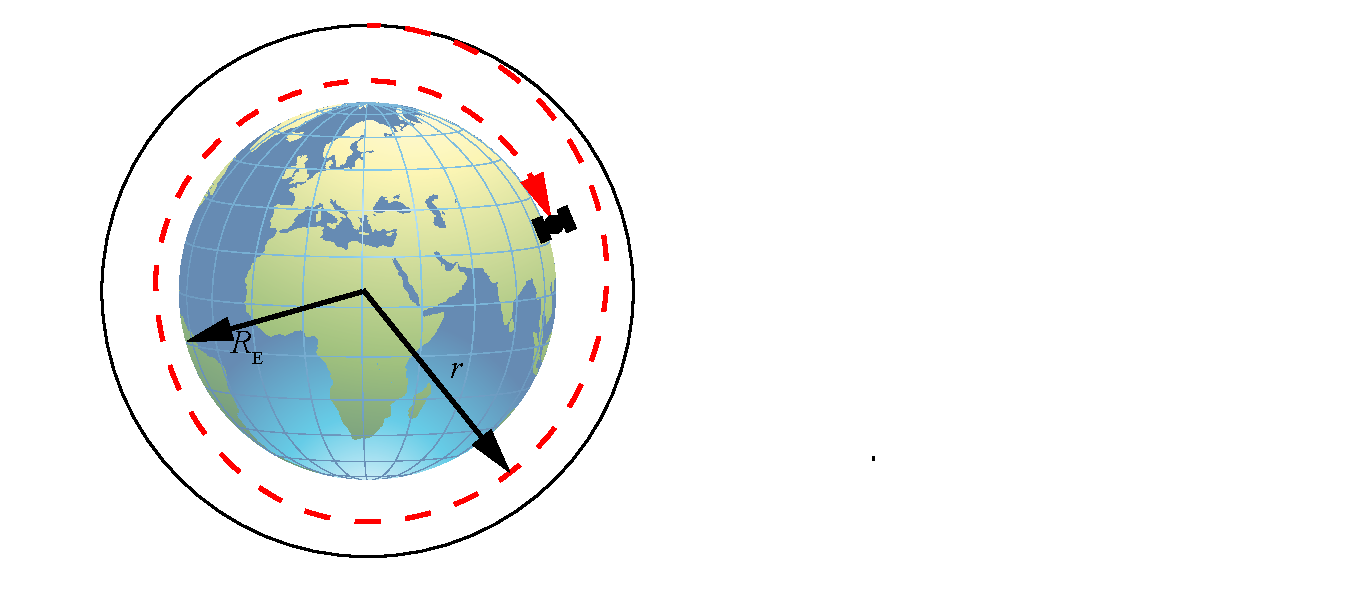
\includegraphics[width=\textwidth]{Tiangong01.pdf}
\caption[Einfaches Modell zur Berechnung des Absturzes des chinesischen Satelliten Tiangong-1.]{Einfaches Modell zur Berechnung des Absturzes des chinesischen Satelliten Tiangong-1.}
\label{abb:adyn_Tiangong01}
\end{figure}


\begin{enumerate}
\item [1.] Wir k�nnen aus \figref{adyn_ISS2004} folgende Raten des Radiusabfalls f�r das Jahr 2014 bestimmen: \\
    \begin{align*}
        \frac{\Delta a}{\Delta t} &= \SI{-1.578e-6}{\km\per\second} \pm \SI{1.0e-6}{\km\per\second} \approx \SI{-130}{\metre\per\day}\pm \SI{80}{\metre\per\day}
    \end{align*}
    Daraus erh�lt man �ber \eqref{eq:adyn_tiangong03} und \eqref{eq:adyn_tiangong05} eine effektive Fl�che 
    \begin{align*}
        A_\text{eff} = \kappa_\text{D}\,A_\perp \approx \SI{210}{\square\metre} \pm \SI{140}{\square\metre}\,,
    \end{align*}
    was eher am unteren Ende der Erwartung liegt, wenn man
    \begin{align*}
        A_\perp \approx
        \begin{cases}
            \SI{50}{\metre}\cdot\SI{70}{\metre} = \SI{3500}{\square\metre}\\
            \SI{109}{\metre}\cdot\SI{51}{\metre} \approx \SI{5000}{\square\metre}
        \end{cases}
    \end{align*}
    entsprechend der Literatur ansetzt, wobei man hierbei das Sonnensegel als voll ausgebreitet in Flugrichtung annimmt. Wir m�ssten dann von einem relativ niedrigen $\kappa_\text{D}$ Wert von $\SI{0.1}{}$ ausgehen. \\
    Fehler in unserer Absch�tzung k�nnen vor allem in der Dichteberechnung liegen. Eine �berpr�fung mit dem Harries-Priester-Modell \cite{Montenbruck2012} ergibt f�r eine H�he von $\SI{420}{\km}$ Werte von $\varrho$ zwischen $\SI{1.558}{\g\per\cubic\km}$ und $\SI{5.684}{\g\per\cubic\km}$ je nach Tageszeit eine etwas bessere �bereinstimmung mit den $A_\text{eff}$-Werten aus der Literatur!\\
    Im Fall eines Magnetsturms kann man von einer Zunahme der Partikeldichte ausgehen, die wegen
    \begin{align*}
        \frac{\Delta a_1/\Delta t}{\Delta a_0/\Delta t} = 4 = \frac{\varrho_1}{\varrho_0}
    \end{align*}
    in etwa proportional zur Zunahme der Rate des Radiusabfalls ist. \\
\item [2.] Wir k�nnten zur Berechnung nat�rlich das Instrumentarium aus \kap{adyn_reentry} benutzen und da insbesondere die Gleichungen \eqref{eq:adyn_reentry02} \bzw \eqref{eq:adyn_reentry02}. Da uns aber wesentliche Informationen fehlen \bzw nicht in ausreichender Genauigkeit vorliegen, wollen wir ein einfaches Modell verwenden. Wir gehen von einer kreisf�rmigen Bahn aus, nehmen an, dass der Drag immer entgegengesetzt zur Richtung der Geschwindigkeit wirkt. Ebenso wird ein konstanter FPA von $\gamma=0$ angenommen. Damit k�nnen wir auch annehmen, dass die Verringerung der Energie des Satelliten (\figref{adyn_Tiangong01}) allein aus der Reibungsarbeit des Drags resultiert, also
    \begin{align}
        \frac{\D}{\D t} H = \frac{\D}{\D t}\lk \frac{\mu_\text{E}\,m_\text{R}}{2r}\rk = F_\text{D}\,v_\text{R}~~~\text{mit}~~~
        F_\text{D} = \frac{1}{2}\,\varrho\lk r\rk \,\kappa_\text{D}\,A_\perp\,v_\text{R}{}^2\,,\label{eq:adyn_tiangong01}
    \end{align}
    worin $\varrho\lk r\rk$ die Dichte der Restatmosph�re im Abstand $r$ vom Erdmittelpunkt und $A_\perp$ die wirksame Fl�che des Raumschiffs senkrecht zur Bewegungsrichtung ist, $\kappa_\text{D}$ ist der Drag-Koeffizient. \\
    Wir erhalten aus \eqref{eq:adyn_tiangong01} die einfache Differentialgleichung 
    \begin{align}
        \begin{split}
            \dot{r} &= -\kappa_\text{eff}\,\sqrt{r}\,\varrho\lk r\rk ~~~~ \text{\bzw mit} ~~~~ r = h + R_\text{E}\, \\
            \dot{h} &= -\kappa_\text{eff}\,\sqrt{h+R_\text{E}}\,\varrho\lk h\rk ~~~~ \text{und}~~~\kappa_\text{eff} = \sqrt{\mu_\text{E}}\,\frac{\kappa_\text{D}\,A_\perp}{m_\text{R}}\,.
        \end{split} \label{eq:adyn_tiangong03}
    \end{align}
    F�r $\varrho\lk h\rk$ benutzen wir ein Modell der Australian Space Weather Agency \cite{Fiolhais2023}:
    \begin{align}
        \varrho\lk h\rk = \SI{6e-1}{} \exp\lk-\frac{\lk h-h_0\rk}{H}\rk\,\SI{}{\kg\per\cubic\km}\label{eq:adyn_tiangong04}
    \end{align}
    mit $H= 29.5 \pm 0.1$ und h=\SI{175}{ \km}.\\
    Da $m_\text{R} = \SI{8.5e3}{\kg}$ bekannt ist, ist der einzig anzupassende Parameter in unserem Modell dann die effektive Fl�che $A_\text{eff} = \kappa_\text{D}\,A_\perp$:
    \begin{align}
        \kappa_\text{eff} = \sqrt{\mu_\text{E}}\,\frac{A_\text{eff}}{m_\text{R}} = \sqrt{\mu_\text{E}}\,\frac{\kappa_\text{D}\,A_\perp}{m_\text{R}}\,. \label{eq:adyn_tiangong05}
    \end{align}
    Wenn wir mit den Anfangswerten f�r Apog�um und Perig�um von $\SI{286}{\km}$ \bzw $\SI{274}{\km}$ eine Anpassung an die experimentellen Werte vornehmen, erhalten wir $A_\text{eff,A} \approx \SI{63}{\square\metre}$ \bzw $A_\text{eff,P} \approx \SI{33}{\square\metre}$, was mit den Abmessungen der Raumstation von $\SI{4}{\metre}\cdot\SI{10}{\metre}$ relativ gut �bereinstimmt (\figref{adyn_Tiangong02}). Gleichwohl ist der Unterschied zwischen den Perig�ums- und Apog�umswerten recht gro�, was aber an unserem einfachen Modell liegt. \\
    Der Leser �berlege sich, ein verbessertes (numerisches) Modell, welches die Elliptizit�t der Anfangsbahn ber�cksichtigt und den Drag dann st�ckweise auf der elliptischen Bahn ber�cksichtigt. Welche weiteren Verbesserungen des Modells sind dar�ber hinaus denkbar und relativ einfach umzusetzen?\\

\begin{figure}[H]
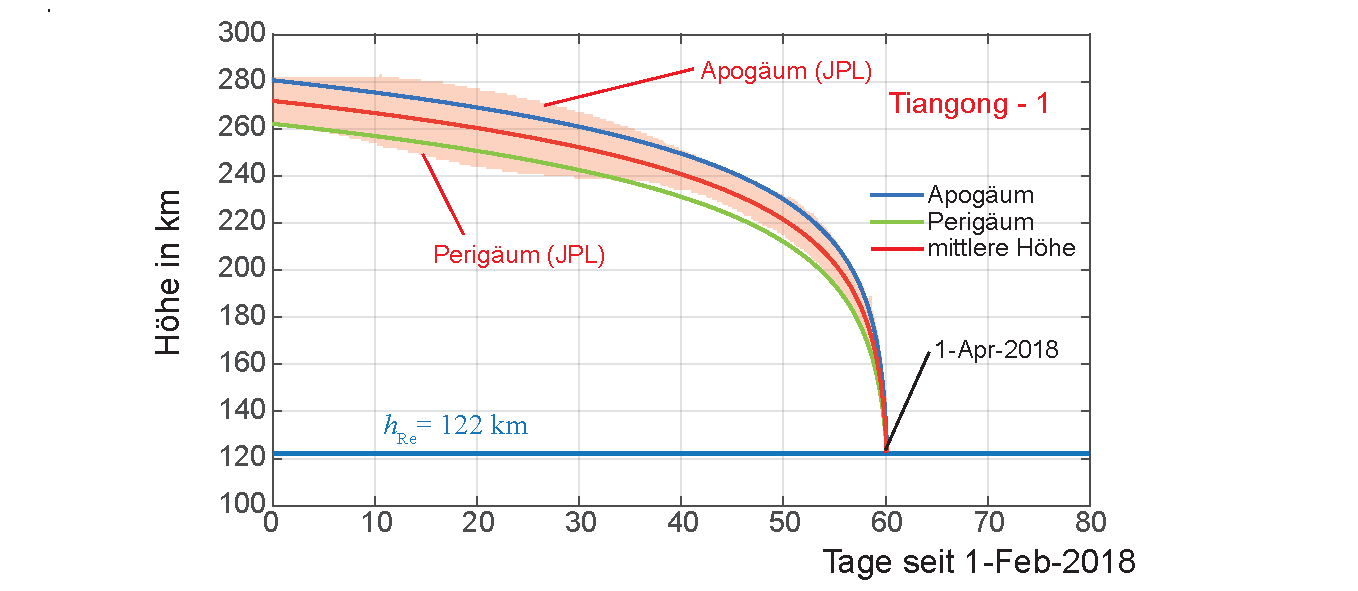
\includegraphics[width=\textwidth]{Tiangong02.pdf}
\caption[Zeitliche Entwicklung des Bahnradius bis zum Absturz des chinesischen Satelliten Tiangong-1.]{Zeitliche Entwicklung des Bahnradius des chinesischen Satelliten Tiangong-1.}
\label{abb:adyn_Tiangong02}
\end{figure}

\end{enumerate}    

Alle Rechnungen sind im \mscr~\mladynref{OrbitalDecay.m} hinterlegt. 

\end{sol} 
\textcolor{blue} {$\rightarrow$ zur} \probref{adyn_reentry04}.\\
\noindent\rule[1ex]{\textwidth}{0.5pt}  \newpage  \clearpage

%-----------------------------------------------------------------------------------------------------------

\begin{sol}{prob:adyn_BoatRocketModel}\label{lsg:adyn_BoatRocketModel} %�bung31
\textbf{Zur Entspannung}\\

Die anf�ngliche Gesamtmasse $M$ besteht aus der Boot- und K�rpermasse $m_\text{B},\, m_\text{L}$, sowie den $N$ Kokosn�ssen mit der Masse $m_\text{K}$ pro Nuss.
    \begin{align}
        M &= m_\text{L} + m_\text{B} + \sum\limits_1^N m_\text{K} \,. \label{eq:adyn_RaketenAlt01}
    \end{align}
F�r jeden Abwurf einer Kokosnuss schreiben wir sukzessive die Geschwindigkeit $V_i$ des Bootes nach Abwurf einer Kokosnuss �ber die Impulserhaltung auf:\\
\underline{1. Abwurf:} 
    \begin{align}
        -m_\text{K}\,v_\text{K} + \lk M-m_\text{K}\rk \,V_1 &= 0 ~~~~
        \rightarrow  ~~~~~ V_1 &= \frac{m_\text{K}}{M-m_\text{K}}\,v_\text{K}\label{eq:adyn_RaketenAlt02}
    \end{align}\\
\underline{2. Abwurf:} 
    \begin{align}
        -m_\text{K}\,\lk v_\text{K} - v_1\rk + \lk M-2m_\text{K}\rk\,V_2 &= \lk M-m_\text{K}\rk\,V_1 ~~~~
        \rightarrow ~~~~ V_2 &= \lek \frac{m_\text{K}}{M-m_\text{K}} + \frac{m_\text{K}}{M-2m_\text{K}}\rek\,v_\text{K} \label{eq:adyn_RaketenAlt03}  
    \end{align}\\
\underline{N-te Abwurf} 
    \begin{align}
        V_N = \sum\limits_{n=1}^N \frac{m_\text{K}\,v_\text{K}}{M-n\,m_\text{K}} = \frac{m_\text{K}\,v_\text{K}}{M}\,\sum\limits_{n=1}^N\,\frac{1}{1-n\,\frac{m_\text{K}}{M}}\label{eq:adyn_RaketenAlt04}  
    \end{align}

Man kann leicht mit \matlab{} zeigen, dass diese Summe konvergiert. Man beachte dabei, dass $N\,m_\text{K} = M-m_\text{L} - m_\text{B}$ ist. \\
F�hren wir die Masse $m_\text{G} = n\,m_\text{K}$ als die Masse der geworfenen Kokosn�sse ein, 
\begin{align}
    V_n &= v_\text{K}\,\sum\limits_{n=1}^N\,\frac{1}{\mu^N-n} ~~~~ \text{mit} ~~~~ \mu = \frac{n\,M_0}{M_\text{T}} = \frac{n\,M_0}{n\,m_\text{K}} ~~~~ \rightarrow ~~~~ \mu = \frac{M_0}{m_\text{K}}>1 \nonumber \\
    &= v_\text{K}\,\lek \frac{1}{\mu-1}+\frac{1}{\mu-2} + \ldots +\frac{1}{\mu-n}\rek \label{eq:adyn_RaketenAlt05}  
\end{align}
Wir bilden nun den Grenzwert:
\begin{align}
    \lim_{N\to\infty} V_N = v_\text{K}\, \lim_{N\to\infty}\sum\limits_{n=1}^N\,\frac{1}{\mu-n}\label{eq:adyn_RaketenAlt06}\,.
\end{align}
Im \mscr ~ \mladynref{AlternativRaketenGL.m} l�sst sich die Grenzwertbildung gut numerisch simmulieren. Das Ergebnis ist in \figref{adyn_RaketenAlternative} gezeigt.\\
Wir ersetzen $\mu = n\,M_0/M_\text{T} = n/x$ mit $0<x=M_\text{T}/M_0<1$:
\begin{align}
    V_N = v_\text{K}\sum\limits_{n=1}^N\,\frac{1}{n/x-n}\,\frac{x}{x} = v_\text{K}\sum\limits_{n=1}^N\,\frac{x}{n-n\,x}\label{eq:adyn_RaketenAlt07}\,.
\end{align}

\begin{figure}[H]
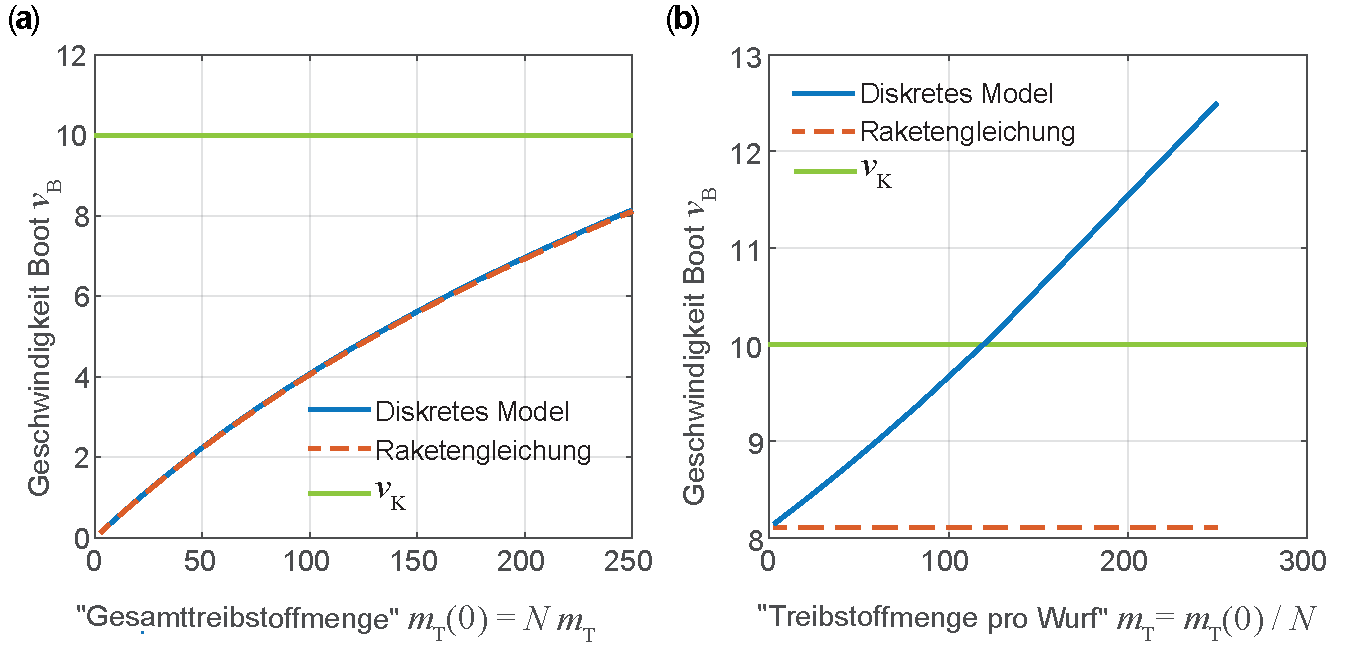
\includegraphics[width=\textwidth]{BoatRocketModelLsg.pdf}
\caption[Diskretes Modell der Raketengleichung.]{Diskretes Modell der Raketengleichung.}
\label{abb:adyn_RaketenAlternative}
\end{figure}


\begin{nebenrechnungNeu} {Grenzwertberechnung}
  
Wir wollen den Grenzwert bilden:
\begin{align}
    \lim_{N\to\infty} V_N &= v_\text{K} \lim_{N\to\infty} \lk \frac{1}{\mu-1} + \frac{1}{\mu-2} + \ldots + \frac{1}{\mu-n}\rk \nonumber \\
    &= v_\text{K} \lim_{N\to\infty} \lk \frac{x}{n-x} + \frac{x}{n-2x} + \ldots + \frac{n}{n-n\,x} \rk = S(x) \label{eq:adyn_RaketenAlt08}
\end{align}
Wir berechnen zun�chst die Partialsumme $S_k^n$, die die Summe aller Terme der Summe $V_n$ nach \eqref{eq:adyn_RaketenAlt08} bis zum $k$-ten Term beinhaltet. Wir definieren dies wie folgt rekursiv:
\begin{align}
    S_{k+1}^n = S_{k}^n + \frac{x}{n-\lk k+1\rk\,x} ~~~~ \text{mit} ~~~~ n=1,2,\ldots,N ~~~~\text{und} ~~~~ k = 0,1,\ldots,\lk n-1\rk\label{eq:adyn_RaketenAlt09}
\end{align}
Dabei ist:
\begin{align*}
    S_0^1 = 0
    \begin{cases}
        n=1,\, k=0
    \end{cases}
    ~~~\text{und}~~~
    S_1^1 = S_0^1 + \frac{x}{1-x} = \frac{x}{1-x}
    \begin{cases}
        n=1,\, k=1
    \end{cases}
\end{align*}
Wir bilden den Quotienten:
\begin{align}
    \frac{S_{k+1}^n - S_k^n}{x/n} = \frac{1}{1-\lk k+1\rk \,x/n}\label{eq:adyn_RaketenAlt10}
\end{align}
und bezeichnen der Einfachheit wegen: 
\begin{align}
    \lk k+1\rk\,\frac{x}{n} = \chi_\text{k} \label{eq:adyn_RaketenAlt11}
\end{align}
und 
\begin{align}
    S_{k+1}^n - S_k^n = \Delta S\lk \chi_\text{k}\rk\,.  \label{eq:adyn_RaketenAlt12}
\end{align}
Damit wird aus \eqref{eq:adyn_RaketenAlt10} der Differentialquotient
\begin{align}
    \frac{\Delta S\lk \chi_\text{k}\rk}{\Delta \chi_\text{k}} = \frac{1}{1-\chi_\text{k}}\,. \label{eq:adyn_RaketenAlt13}
\end{align}
Wir bilden den Grenzwert $n\to\infty$ und erhalten mit $S\lk \chi_\text{k}\rk$ das Riemann-Integral der rechten Seite:
\begin{align}
    S\lk \chi_\text{k}\rk = -\ln\lk 1-\chi_\text{k}\rk = \ln \lk \frac{1}{1-\chi_\text{k}}\rk\,. \label{eq:adyn_RaketenAlt14}
\end{align}
Mit \eqref{eq:adyn_RaketenAlt11} k�nnen wir f�r $n\to\infty$ auch schreiben ($k=n,\,\chi_\text{k}\to x$)
\begin{align*}
    S\lk \chi_\text{k}\rk = S\lk x\rk
\end{align*}
also:
\begin{align}
    \ln\lk \frac{1}{1-x}\rk = \lim_{n\to\infty} \lk \frac{x}{n-x} + \frac{x}{n-2x} +\ldots + \frac{x}{n-n\,x}\rk\,. \label{eq:adyn_RaketenAlt15}
\end{align}
Damit wird aus \eqref{eq:adyn_RaketenAlt11}
\begin{align}
    V= \lim_{n\to\infty} V_N = v_\text{k}\,\ln\lk\frac{1}{1-x}\rk = v_\text{k}\,\ln\lk\frac{1}{1-M_\text{T}/M_0}\rk = v_\text{k} \,\ln\frac{M_0}{M_0-M_\text{T}}\,, \label{eq:adyn_RaketenAlt16}
\end{align}
was genau der Raketengleichung \eqref{eq:adyn_rocketequ} entspricht. (Diese Rechnung wurde in �hnlicher Form zuerst in \cite{Lagos2023} gezeigt.)\\

\end{nebenrechnungNeu}


\end{sol} 
\textcolor{blue} {$\rightarrow$ zur} \probref{adyn_BoatRocketModel}.\\
\noindent\rule[1ex]{\textwidth}{0.5pt}  \newpage  \clearpage

%-----------------------------------------------------------------------------------------------------------
%-----------------------------------------------------------------------------------------------------------

\newpage
\subsection{Weiterf�hrende Zusatzaufgaben und Probleme}

\begin{sol}{prob:adyn_launchinnovations}\label{lsg:adyn_launchinnovations} %Zusatz1
\textbf{Neue Ideen zum Flug ins Weltall}\\

Wir zitieren aus der etwas sp�rlichen Information der Firma Spinlaunch (\url{www.spinlaunch.com}):
\begin{quotation}
\textit{The Suborbital Accelerator is designed to operate from 800 to 5,000 mph (approx. 8000 km/h) and acts primarily as a test-bed for the Orbital Launch System. On October 22nd, 2021, our first launch successfully propelled a test vehicle at supersonic speeds and ended with the recovery of the reusable flight vehicle. Throughout 2022 the system will conduct regular test flights with a variety of vehicles and launch velocities. The Suborbital System offers testing capabilities to customers and provides long term value as a satellite qualification facility.
}
\end{quotation}
So weit so gut. Schauen wir uns diese neueren Ideen f�r den Weltraumflug genauer an:\\
Den Weltraumfahrstuhl haben wir bereits in �bung 1.10 von Band I untersucht und verweisen daher auf die entsprechende L�sung.\\
Die \anf{Weltraumachterbahn}, wie der Spinlaunch auch genannt wird, ist ein neues Konzept und wir wollen uns die Machbarkeit unter drei Gesichtspunkten genauer anschauen. Wir benutzen dabei Angaben, die von der Fa. SpinLaunch \bzw in der Literatur im Internet zu finden sind.\\
Danach soll der Raumtransporter (Anfangsmasse von $m_0 = \SI{250}{\kg}$) die Zentrifuge mit einer Geschwindigkeit von $\SI{1000}{}$ - $\SI{8000}{\km\per\hour}$ verlassen und ohne Antrieb eine H�he von $\SI{60}{\km}$ �ber der Erdoberfl�che erreichen, wo eventuell noch einmal mit einer mitgenommenen Treibstoffmenge von $\SI{100}{\kg} \ldots \SI{150}{\kg}$
eine weitere Beschleunigung erfolgen kann. 
Der Durchmesser der Zentrifuge betr�gt etwa  $D=2R=\SI{50}{\metre}$.\\
Wir wollen untersuchen:
\begin{itemize}
    \item [1)] 
    \textbf{\textit{Mechanische Herausforderungen an die Zentrifuge}}:\\
    Es gilt: $v_0 = \omega\,D \quad \rightarrow \quad \omega = v_0/D$.\\
    Mit den geforderten Werten erhalten wir $\omega \approx 120,\ldots,1000\,\SI{}{\per\second}$.\\
    Wir gehen davon aus, dass das Raumschiff durch ein Gest�nge in der Zentrifuge geleitet wird. Das Gest�nge soll einen effektiven Durchmesser von $D = \SI{0.5}{\metre}$ haben und aus Stahl \bzw Kohlenfaserverbundstoffen bestehen.\\
    Die gesamte Zugspannung auf das Gest�nge  betr�gt dann:
    \begin{align*}
        \sigma = A\,\varrho\,\frac{R^2}{2}\,\omega^2 + m_0\,\omega^2\,\frac{R}{A} 
    \end{align*}
mit $A=\pi D^2/4$  und $\varrho \approx \SI{7e3}{\kg\per\cubic\metre}\,\text{(Stahl)}\, \text{\bzw}\, \varrho = \SI{2e3}{\kg\per\metre}\,\text{(Kohlenfaser)}$.  Wir erhalten\\
$\sigma = \SI{6.6}{\giga\Pa}$ (Stahl) \bzw $\sigma= \SI{2.2}{\giga\Pa}$ (Kohlenfaser).\\
Diese Werte sind dicht an der maximal erreichbaren Zugspannung vor einer m�glichen Zerst�rung. Hierin liegt also eine erste Herausforderung in der Lagerung des Zentrifugalarms, diese enormen Radialkraft muss ja durch das Lager aufgenommen werden.\\
    \item [2)]
    \textbf{\textit{Antriebsloser Aufstieg}}:\\
Nach Ausl�sen aus der Zentrifuge tritt der  Raumtransporter aus dem Vakuum in die Erdatmosph�re und erf�hrt auf dem Weg nach oben neben den gravitativen Verlusten auch Reibungsverluste.\\
    Wir k�nnen die Ergebnisse von \probref{adyn_launch01} benutzen und erhalten unter der Annahme von optimistischen Werten von $c_\text{w,R} = 0.2$ und $A_\text{R} = \pi\,\SI{0.25}{\square\metre}/4$ eine maximale H�he am Ende der Spin Launch Phase von $h_\text{end} = \SI{50}{\km},\ldots,\SI{60}{\km}$ \bzw eine Geschwindigkeit von $v_\text{end}\lk h=\SI{60}{\km}\rk\approx \SI{1.25}{\km\per\second}$.\\
    \item [3)]
    \textbf{\textit{Zusatzschub}}:\\
    Nimmt man an, dass bei $h=\SI{60}{km}$ noch $\SI{200}{\kg}$ Treibstoff mit $v_\text{G}=\SI{5000}{\metre\per\second}$ (sehr optimistisch) zur Verf�gung stehen, dann hat man dort f�r die verbleibende Nutzlast von $\SI{100}{kg}$ (ohne Strukturmasse) noch ein Geschwindigkeitsbudget von
    \begin{align*}
        \Delta v = v_\text{G}\,\ln\,\frac{m_\text{L}}{m_0}\, = \SI{5.9}{\km\per\second}
    \end{align*}
    zur Verf�gung, zus�tzlich der 
    \begin{align*}
        \Delta v_\text{E} \approx \SI{0.4}{\km\per\second}
    \end{align*}
    aus der Rotation der Erde.\\
    Gebraucht werden f�r eine Kreisbahn in $\SI{200}{\km}$:
    \begin{align*}
        v_\text{k} =  \sqrt{ \frac{\mu_\text{E}}{R_\text{E}}+\SI{200}{\km}}\approx \SI{7.85}{\km\per\second}\,,
    \end{align*}
    \dh unter den Annahmen kommt es zu keiner stabilen Kreisbahn in $\SI{200}{\km}$ H�he, es wird sich also um einen suborbitalen Flug handeln.\\
		\item [4)] 
    Wir wollen nun noch die energetischen Verh�ltnisse betrachten.\\
    Um eine Nutzlast von $\SI{100}{\kg}$ mit in eine H�he von $\SI{200}{\km}$ zu bringen, braucht man (ohne Ber�cksichtigung der Unterst�tzung durch die Erdrotation) ein Geschwindigkeitsbudget von 
    \begin{align*}
        \Delta v = \SI{7.85}{\km\per\second}
    \end{align*}
    \bzw bei Annahme einer Strukturmasse von $\SI{500}{\kg}$ eine Treibstoffmasse von 
    \begin{align*}
        m_\text{T} = m_\text{L} \, \lk \e^{+\frac{\Delta v}{v_\text{G}}} - 1 \rk - m_\text{S} \approx \SI{300}{\kg}\,.
    \end{align*}
    Man spart also in etwa $\SI{100}{\kg}$ Treibstoff. Daf�r muss man durch elektrischen Antrieb eine kinetische und Rotationsenergie von 
    \begin{align*}
        T = \frac{m_0}{2}\,v_0{}^2 + \frac{J}{2}\,\lk\frac{v_0}{R}\rk^2 = \frac{1}{2}\,v_0{}^2\,\lk m_0 + \frac{J}{R^2} \rk
    \end{align*}
    aufbringen, wenn $J$ das Tr�gheitsmoment des Rotationsarms ist.
    \begin{align*}
        J &= \frac{1}{3}\,m_{\text{Rotor}}\,R^2 = \frac{1}{3}\,\frac{\pi}{4}\,D^2\,R^3 \,\varrho \approx \SI{1.8}{\kg\square\metre}\\
        \rightarrow \quad T & \approx \SI{5.8}{\N\metre} \approx \SI{1.6}{\mega\watt\hour}
    \end{align*}
    Der \anf{eingesparte} Treibstoff (typische Parameter) hat einen \anf{Energieinhalt} von
    \begin{align*}
        E_{\text{chem}} &= \epsilon_\text{T}\,\Delta m_\text{T}\\
        &\approx \SI{3500}{\kilo\joule\per\mol}\cdot\SI{0.01}{\mol\per\g}\cdot\SI{100e3}{\g} \approx \SI{3.5e9}{\joule} \approx \SI{1}{\mega\watt\hour}
    \end{align*}
    Auch daran sieht man, dass man energetisch nicht wirklich etwas spart (wie k�nnte man auch?), jedoch w�re der Betrieb der SpinLaunch-Anlage nat�rlich mit \anf{nachhaltiger} Energie machbar.\\
    \item [5)]
    \textbf{\textit{Zusammenfassung}}:\\
    Alles in allem sieht das Projekt SpinLaunch etwas erfolgversprechender aus als der Erdfahrstuhl, wenngleich die ingenieurtechnischen Anforderungen riesig sind und auch der f�r 2022 angek�ndigte Erstflug bislang nicht erfolgt ist. \\
    In \figref{adyn_SpinLaunch} haben wir das Ergebnis der Simulation eines SpinLaunch-Unternehmens f�r eine Nutzlast von \SI{100}{\kg} und einem \textit{on-board} Treibstoffvorrat von $\SI{200}{\kg}$ dargestellt. Auch sonst sind alle anderen Annahmen extrem optimistisch gemacht. Man erkennt, dass dieses Prinzip bestenfalls f�r kleinere Nutzlasten machbar/sinnvoll erscheint, wobei wir mal von den \anf{kleinen} ingenieurtechnischen Herausforderungen wie Vakuum f�r die Zentrifuge, Stabilit�t der Materialien, Bewegung von $\SI{200}{\kg}$ Treibstoff bei einer \anf{leicht erh�hten} Zentrifugalbeschleunigung von $a_\text{z} = v_0{}^2/R\approx \SI{20e3}{} g$ absieht.
\end{itemize}


\begin{figure}
	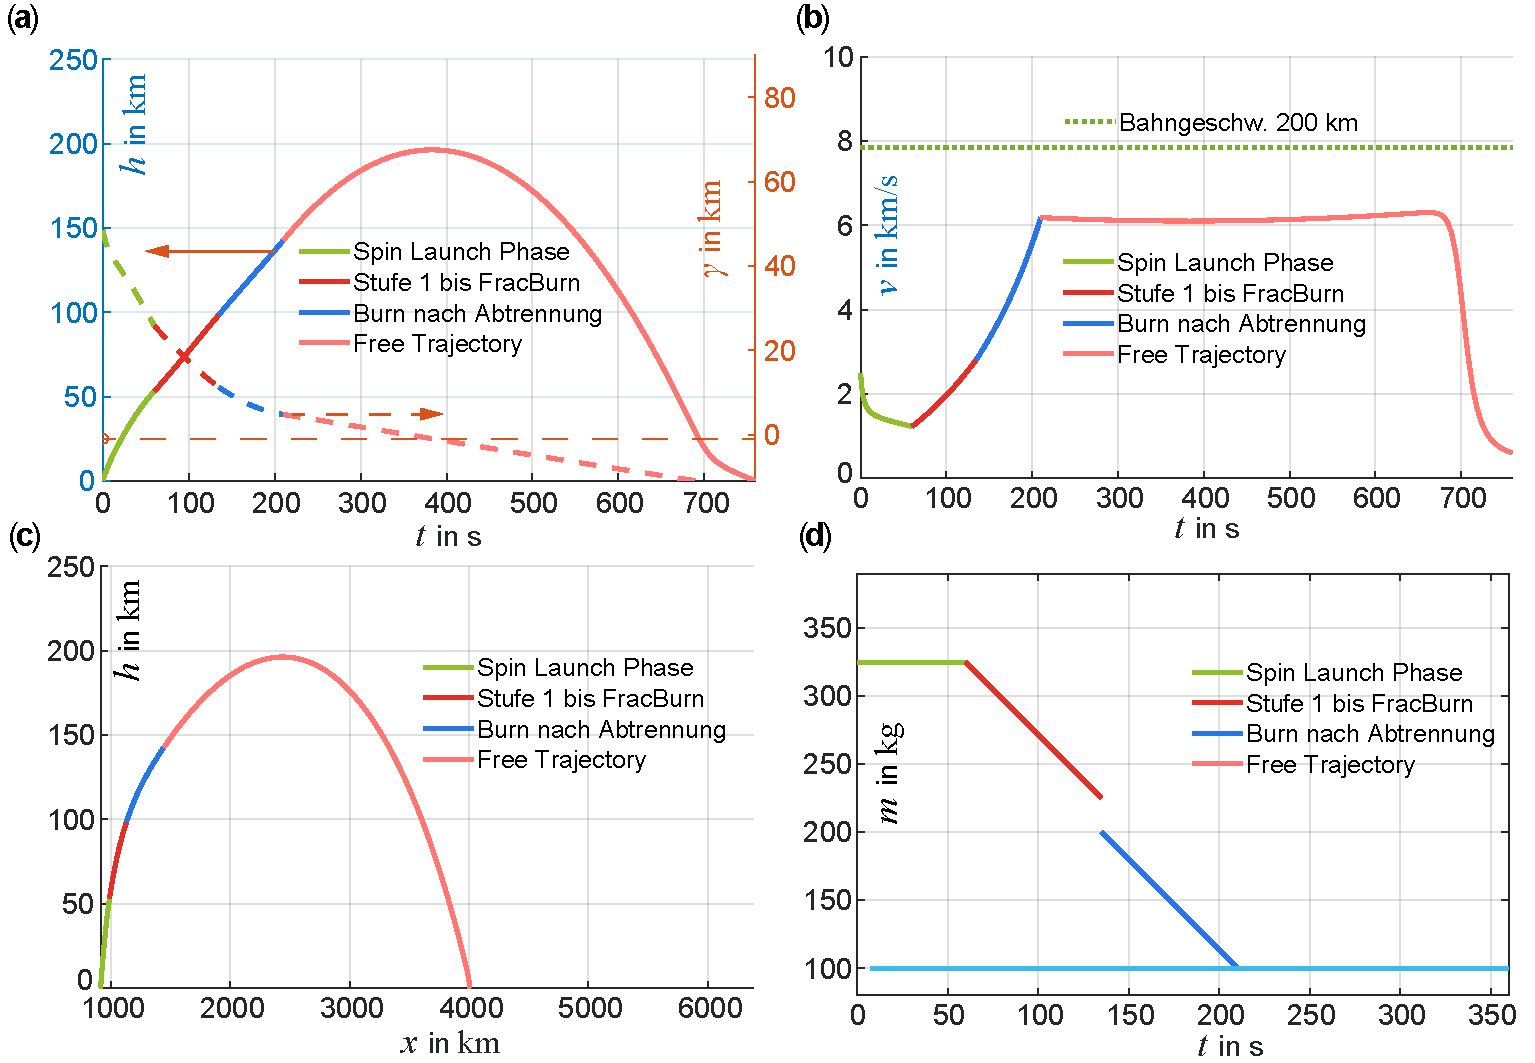
\includegraphics[width=\textwidth]{Spinlaunch.pdf} 
	\caption[Beispielrechnungen zum Spinlaunch.]{Beispielrechnungen zum Spinlaunch. Parameter siehe Text und \mscr~\mladynref{Spinlaunch.m} \fa H�he und FPA �ber die Zeit \fb Geschwindigkeit �ber die Zeit \fc H�he �ber Horizontkoordinate $x$ \fd Masse des Raumtransporters �ber die Zeit.}
	\label{abb:adyn_SpinLaunch}
\end{figure}

\end{sol} 
\textcolor{blue} {$\rightarrow$ zur} \probref{adyn_launchinnovations}.\\
\noindent\rule[1ex]{\textwidth}{0.5pt} \newpage  \clearpage


%-----------------------------------------------------------------------------------------------------------

\begin{sol}{prob:adyn_orbits_zusatz2}\label{lsg:adyn_orbits_zusatz1} %Zusatz
\textbf{Bahnparameter aus Bodenbeobachtungen (Ortsvektoren)}\\

Zun�chst m�ssen wir aus den topozentrischen Messwerten ($\vec{R}$ mit Distanz $R$, Azimut $\mathcal{A}$ und H�he $h$) geozentrisch-�quatoriale Messwerte "`machen"'. Wir invertieren dazu \eqref{eq:adyn_statobserv06} und erhalten:
\begin{align}
	  \vec{r} =  \mathbb{R}_\text{z}\lk -\theta\rk \, \lek \mathbb{U}^{-1} \,\vec{R} + \vec{r}_\text{B} \rek \,, \label{eq:adyn_bahnbest_lsg01}
\end{align}
worin $\vec{r},\, \vec{r}_\text{B}$ die geozentrische-�quatorialen Koordinatenvektoren f�r Satellit und Beobachtungsstation sind und  $\vec{R}$ die topozentrischen Koordinaten des Satelliten.\\
Mit den so bestimmten Vektoren $\vec{r}_1$ und $\vec{r}_2$ zu den beiden Messzeiten /$t_1,$ und $t_2$ kann man nach einer von Gau� entwickelten geometrisch-iterativen Methode die Bahnparameter bestimmen. Im folgenden ist diese der Darstellung in \cite{Montenbruck2012} folgend skizziert. Wir starten mit \figref{adyn_orbit_determination} und gehen wie folgt vor:

\begin{figure}
	\includegraphics[width=\textwidth]{BestimmungOrbitsGauss.pdf} 
	\caption[Bestimmung von Bahnparametern von Satelliten.]{Zur Bestimmung von Bahnparametern von Satelliten aus Orts- und Winkelbeobachtungen.}
	\label{abb:adyn_orbit_determination}
\end{figure}

\begin{enumerate}
    %1
    \item Man benutzt, dass die Bahnebene eines Satelliten immer durch die Ebene gegeben ist, die durch die beiden Vektoren $\vec{r}_1$, $\vec{r}_2$ aufgespannt wird. \\
    Man bestimmt dann �ber die Einheitsvektoren 
    \begin{align}
        \vec{e}_1 &= \frac{\vec{r}_1}{|\vec{r}_1|}~~~~ \text{und} ~~~~ \vec{e}_0 = \frac{\vec{r}_0}{|\vec{r}_0|} \label{eq:adyn_bahnbest_15}
    \end{align}
    mit $\vec{r}_0 = \vec{r}_2 - \lk \vec{r}_2\,\vec{e}_1\rk\,\vec{e}_1$ und den Gau�-Vektor \\
   \begin{align}
			\vec{W} &= \vec{L}/|\vec{L}| = \vec{e}_1\times \vec{e}_0 =\begin{pmatrix} W_x\\W_y\\W_z \end{pmatrix} \,, \label{eq:adyn_bahnbest_15a}
	\end{align}
		der senkrecht auf der Bahnebene steht.\\
    %2
    \item Wir erhalten damit sofort die Inklination 
    \begin{align}
        i = \arctan \lk\frac{\sqrt{W_x{}^2+W_y{}^2}}{W_z}\rk \label{eq:adyn_bahnbest_16}
    \end{align}
    und die Rektaszension des aufsteigenden Knotens 
    \begin{align}
        \Omega = \arctan \lk\frac{W_x}{-W_y}\rk \,. \label{eq:adyn_bahnbest_17}
    \end{align}
    Ebenso bestimmt man das Argument der L�nge, welches wir sp�ter noch ben�tigen: 
    \begin{align}
        u_1 =\arctan\lk\frac{z_1}{-x_1\,W_y +y_1\,W_x}\rk\,. \label{eq:adyn_bahnbest_17a}
    \end{align}
    %3
    \item Zur Bestimmung der restlichen Bahnparameter braucht man einige Hilfsgr��en, wir verweisen f�r eine detailliertere Darstellung auf die Literatur \cite{Montenbruck2012, Bucerius1950, Escobal1965}. \\
		
		Mit dem Bahnparameter $p$ der Ellipse $p=a\,(1-e^2) $ findet man die Sektorenfl�che nach dem 2. Keplerschen Gesetz (\figref{adyn_orbit_determination}a zu:
    \begin{align}
        A_\text{S} = \frac{1}{2} \sqrt{G\,m_\text{E}}\,a\,(1-e^2)\,\lk t_2 -t_1\rk  \,. \label{eq:adyn_bahnbest_19a}
    \end{align}
		Die entsprechende durch $\vec{r}_1$ und $\vec{r}_2$ definierte Dreiecksfl�che nach \figref{adyn_orbit_determination}b ist:
		    \begin{align}
        A_\Delta = \frac{1}{2}\,r_1\,r_2\,\sin\lk \upsilon_2-\upsilon_1\rk= \frac{1}{2}\,r_1\,r_0 \,.\label{eq:adyn_bahnbest_19b}
    \end{align}
		Ferner setzen wir 
    \begin{align}
        \tau = \sqrt{G\,m_\text{E}}\,\lk t_2 -t_1\rk  \label{eq:adyn_bahnbest_20a}
    \end{align}
		 als eine mit $\sqrt{G\,m_\text{E}}$ multiplizierte Zeit zwischen den zwei Messungen. Wir definieren nun die Gr��e  $\eta$ als das  Verh�ltnis von Sektorfl�che $A_\text{S}$ zu Dreiecksfl�che $A_\Delta$ und erhalten:
    \begin{align}
        \eta = \frac{A_\text{S}}{A_\Delta} = \frac{\sqrt{p}\,\tau}{r_1\,r_2\,\sin(\upsilon_2 - \upsilon_1)} \label{eq:adyn_bahnbest_20b}
    \end{align}
		Hat man $\eta$ berechnet, kann man �ber   
    \begin{align}
        p = \lk \frac{2\,A_\Delta\,\eta}{\tau} \rk^2\,, \label{eq:adyn_bahnbest_18}
    \end{align}
    den Parameter $p$ der Bahnellipse bestimmen. Dieser, wie auch die wahren Anomalien, sind aber noch unbekannt, ebenso wie $\eta$. Ersetzt man diese durch die Gr��en aus der Bahngleichung \bzw Kepler-Gleichung, wobei man mit $\zeta = \lk E(t_2) - E(t_1) \rk /2 $ eine Hilfsgr��e einf�hrt, erh�lt man f�r $\eta$ und $\zeta$ das folgende nichtlineare Gleichungssystem 
    \begin{align}
    \begin{split}
        \eta^2\,\lk \eta-1\rk &= m\,\frac{2\zeta -\sin\lk 2\zeta\rk}{\sin^3\lk\zeta\rk}\,, \\
        \eta^2 &= m\,\frac{1}{k+\sin^2\lk \zeta/2 \rk}
    \end{split} \label{eq:adyn_bahnbest_21}
    \end{align}
		mit den Abk�rzungen f�r die Kombination der bekannten Gr��en $\vec{r}_1, \vec{r}_2$:
    \begin{subequations}
    \begin{align}
        m &= \frac{\tau^2}{\sqrt{2\,\lk r_1\,r_2 + \vec{r}_1\,\vec{r}_2\rk}^3}  ~~~\text{und} \label{eq:adyn_bahnbest_22a}\,, \\
        k &= \frac{r_1+r_2}{2\sqrt{2\,\lk r_1\,r_2 + \vec{r}_1\,\vec{r}_2\rk}}-\frac{1}{2}\,. \label{eq:adyn_bahnbest_22b}
    \end{align}
    \end{subequations}
		Die L�sung des nichtlinearen Gleichungssystems \eqref{eq:adyn_bahnbest_21} ergibt sowohl $\eta$ als auch $\zeta$, wobei man eigentlich nur $\eta$  f�r die weitere Berechnung braucht.\\
    %4
    \item Die numerische L�sung f�r $\eta$ findet man mit \matlab �ber drei Wege:		
		\begin{enumerate}
			\item [a)] Man l�st das nichtlinearen Gleichungssystems \eqref{eq:adyn_bahnbest_21} mit Hilfe des \matlab-Solvers \textcolor{mygreen}{\texttt{fsolve}}. Hierzu 
			muss eine Vektorfunktion $\vec{F}_2 = \mathrm{func2d}(\vec{x})$ der Vektorvariablen $\vec{x} = [x(1), x(2)] = [\eta, \zeta]$ definiert werden.
			\item [b)] Man eliminiert aus dem nichtlinearen Gleichungssystems \eqref{eq:adyn_bahnbest_21} die Variable $\zeta$ und erh�lt die Funktion 
			 \begin{align}
				  F_1 &= \mathrm{func1d}(\eta) = 1 - \eta + \frac{m}{\eta^2}\,\frac{2q(\eta)-\sin\lk 2q(\eta) \rk}{\sin\lk q(\eta) \rk^3}~~~\text{mit}~~\label{eq:adyn_bahnbest_23a}\\
					~q &= 2\asin\lk \frac{m}{\eta^2} - k \rk \,, \nonumber 
			 \end{align}
			deren Nullstelle man mit Hilfe des \matlab-Solvers \textcolor{mygreen}{\texttt{fzero}} sucht. 
			\item [c)q] Man startet mit \eqref{eq:adyn_bahnbest_23a} und bestimmt die Nullstelle durch eine Iteration nach folgendem Iterationsschema \cite{Montenbruck2012}:
    \begin{align}
        \eta_{i+1} = \eta_i -f\lk\eta_i\rk\,\frac{\eta_i -\eta_{i-1}}{f\lk \eta_i\rk - f\lk\eta_{i-1}\rk} \label{eq:adyn_bahnbest_23b}
    \end{align}
    mit 
    \begin{subequations}
    \begin{align}
        f\lk\eta_i\rk &= 1-\eta_i + \frac{m}{\eta_i{}^2}\,\lek \frac{4}{3} + \frac{4\cdot 6}{3\cdot 5}\,\lk\frac{m}{\eta_i{}^2}-k\rk + \frac{4\cdot 6\cdot 8}{3\cdot 5\cdot 7}\,\lk\frac{m}{\eta_i{}^2}-k\rk^2 +\ldots\rek\label{eq:adyn_bahnbest_24a}
    \intertext{und den Anfangswerten}
        \eta_0 &= \frac{12}{22} + \frac{10}{22}\,\sqrt{1+\frac{44}{9}\,\frac{m}{k+\frac{5}{6}}} \label{eq:adyn_bahnbest_24b}\\
        \eta_1 &= \eta_0 + 0.1  \label{eq:adyn_bahnbest_24c}
	 \end{align}
    \end{subequations}
		\end{enumerate}
    %5
    \item  Hat man nach einer der drei Methoden $\eta$ berechnet, kann man �ber \eqref{eq:adyn_bahnbest_18} den Ellipsen-Parameter $p$ bestimmen und �ber die Ellipsengleichung 
		\begin{align*}
        e\,\cos\lk\upsilon_1\rk = \frac{p}{r_1}-1\,,~~~ e\,\cos\lk\upsilon_2\rk = \frac{p}{r_2}-1
    \end{align*}
    folgende Bestimmungsgleichungen f�r $\upsilon_1$ und $e$ erhalten:
    \begin{subequations}
    \begin{align}
        e\,\cos\lk\upsilon_1\rk &= \frac{p}{r_1}-1 \label{eq:adyn_bahnbest_25a}\,,\\
        e\,\sin\lk\upsilon_1\rk &= \frac{\lk \frac{p}{r_1}-1\rk\,\lk \frac{\vec{r}_2\,\vec{e}_1}{r_2}\rk-\lk\frac{p}{r_2}-1\rk}{\frac{r_0}{r_2}} \,,\label{eq:adyn_bahnbest_25b}
    \end{align}
    \end{subequations}
    woraus folgt:
    \begin{align}
        \upsilon_1 = \arctan{\lek \frac{\lk \frac{p}{r_1}-1 \rk \, \lk \frac{\vec{r}_2\,\vec{e}_1}{r_2}\rk-\lk\frac{p}{r_2}-1\rk}{\frac{r_0}{r_2}\,\lk\frac{p}{r_1}-1\rk} \rek}
				\label{eq:adyn_bahnbest_26a}
    \end{align}
    \bzw
    \begin{align}
        e = \sqrt{\lk \frac{p}{r_1}-1 \rk^2 + \frac{\lk \lk \frac{p}{r_1}-1\rk\,\lk \frac{\vec{r}_2\,\vec{e}_1}{r_2}\rk-\lk\frac{p}{r_2}-1\rk\rk^2}{\lk \frac{r_0}{r_2}\rk^2}} \,.\label{eq:adyn_bahnbest_26b}
    \end{align}
		%6
    \item Das Argument des Perig�ums $\omega$ bestimmt man �ber 
    \begin{align}
        \omega = u_1 -\upsilon_1 ~~~\text{mit dem Argument der L�nge}~~u_1 = \arctan \lk \frac{z_1}{-x_1\,W_y + y_1\,W_x} \rk \label{eq:adyn_bahnbest_26c}
    \end{align}
    und die gro�e Halbachse $a$ �ber
    \begin{align}
        a = \frac{p}{1-e^2}\,.  \label{eq:adyn_bahnbest_26d}
    \end{align}
    %7
    \item Als sechstes und letztes Bahnelement berechnet sich die mittlere Anomalie zum Zeitpunkt $t_1$ �ber die Kepler-Gleichung 
    \begin{align}
        M_1= E_1 -e\,\sin E_1 \label{eq:adyn_bahnbest_26e}
    \end{align}
    mit der exzentrischen Anomalie 
    \begin{align}
        E_1 = \arctan \lk\frac{\sqrt{1-e^2}\,\sin\upsilon_1}{\cos\upsilon_1 +e}\rk\,. \label{eq:adyn_bahnbest_26f}
    \end{align}
\end{enumerate} 

Die Rechnungen sind im Detail im \mscr~\mladynref{BahnparaBestimmung02.m} hinterlegt.\\

\textbf{Hinweis:} Man muss bei der Bestimmung der Bahnparameter etwas aufpassen, ob die Beobachtungszeiten zum gleichen Umlauf geh�ren oder ob der Satellit inzwischen nicht bereits eine oder mehrere Erdumrundungen vollzogen hat. Im angegebenen Beispiel relativ kurzer Zeiten zwischen zwei Beobachtungen ist sicher davon auszugehen, dass die Daten zum gleichen Umlauf geh�ren.\\

\textbf{Zusatzaufgabe:} In \kap{adyn_lambert_transfer} bzw \probref{adyn_manoevers4} haben wir bei der Behandlung des Lambert-Problems noch eine andere Methode kennen gelernt, wie das Problem der Bestimmung der Bahnparameter  gel�st werden kann. Hierzu bestimmt man aus den gemessenen $\vec{r}_1$ und $\vec{r}_2$ den Winkel $\gamma$ und nimmt als Flugzeit (TOF) des Satelliten auf seine Bahn die Differenz der Beobachtungszeiten. Wir empfehlen zur Vertiefung auch diese Aufgabe hier mit der Methode des Lambert-Transfers zu l�sen.

\end{sol} 
\textcolor{blue} {$\rightarrow$ zur} \probref{adyn_orbits_zusatz2}.\\
\noindent\rule[1ex]{\textwidth}{0.5pt}  \newpage  \clearpage
%
%%-----------------------------------------------------------------------------------------------------------------------------------------------


\begin{sol}{prob:adyn_orbits_zusatz2}\label{lsg:adyn_orbits_zusatz2} %Zusatz
\textbf{Bahnparameter aus Bodenbeobachtungen (Ortsvektoren)}\\

Wir verweisen auf das \mscr~ \mladynref{BahnparaBestimmung03.m}.

\end{sol} 
\textcolor{blue} {$\rightarrow$ zur} \probref{adyn_orbits_zusatz2}.\\
\noindent\rule[1ex]{\textwidth}{0.5pt} \newpage  \clearpage

%-----------------------------------------------------------------------------------------------------------------------------------------------

\begin{sol}{prob:adyn_swingby02}\label{lsg:adyn_swingby02} %Zusatz
\textbf{Gravity-Assist-Man�ver - Allgemeiner Fall}\\

\begin{figure}
	\includegraphics[width=\textwidth]{GeschwindigkeitenSOI.pdf} 
	\caption[Geometrie und Geschwindigkeiten beim Gravity-Assist-Man�ver am Punkt $\mathrm{P}_1$.]{Geometrie und Geschwindigkeiten beim Gravity-Assist-Man�ver am Punkt $\mathrm{P}_1$. Bahnebene des Swing-By und Planetenbahnebene fallen hier gem�� Annahme noch zusammen. }
	\label{abb:adyn_swby01}
\end{figure}

\begin{enumerate}
    %1
    \item [1)]
		Wir definieren zun�chst die Vektoren im Inertialsystem (\figref{adyn_swingby01} und \figref{adyn_swby01}):
    \begin{align*}
        \vec{r}_\text{P} \quad &\text{Vektor zum Planeten} \\
        \vec{r}_\text{R} \quad &\text{Vektor zum Raumschiff} \\
        \vec{v}_1 \quad &\text{Geschwindigkeit des Raumschiffs beim Eintreffen an der SOI des Planeten}\\
        \vec{v}_\text{P} \quad &\text{Geschwindigkeit des Planeten}
    \end{align*} 
    %2
    \item [2)]
    Wir definieren die Geschwindigkeit und den Abstand zum Planeten beim Eintreffen an der SOI im planetozentrischen \KOS:
    \begin{align}
    \begin{split}
        \vec{r}_1{}' &= \vec{r}_\text{R} - \vec{r}_\text{P}\,, \\
        \vec{v}_1{}' &= \vec{v}_1 - \vec{v}_\text{P}\,, \\
              v_1{}' &= |\vec{v}_1{}'| = v_\infty\,, \\
    \end{split} \label{eq:adyn_swby01}
    \end{align}
    Wir wollen dabei zun�chst gem�� \figref{adyn_swby01} noch die Vereinfachung machen, dass die Orbitalebene des Planeten mit der Swing-By Ebene zusammenf�llt, wir werden sp�ter weiter unten diese Einschr�nkung fallen lassen (siehe dazu auch \figref{adyn_GA3dim}).
    %3
    \item [3)]
    Den vektoriellen Sto�parameter $\vec{b}$ k�nnen wir dann ebenfalls definieren, er ergibt sich nach einfachen geometrischen �berlegungen aus \figref{adyn_swby01} zu
     \begin{align}
     \begin{split}
         \vec{b} & =\vec{r}_1{}' + \frac{\vec{v}_1{}'}{v_1{}'^2}\,\lk -\vec{r}_1{}'\cdot\vec{v}_1{}' \rk = \vec{r}_1{}' - \frac{\vec{v}_1{}'}{v_1{}'^2}\,\lk \vec{r}_1{}'\cdot\vec{v}_1{}' \rk \,.
     \end{split}
     \label{eq:adyn_swby02}
     \end{align}
		
\begin{figure}
	\includegraphics[width=\textwidth]{SwingByHyperbel.pdf} 
	\caption[Ablenkwinkel beim Gravity-Assist-Man�ver.]{Ablenkwinkel beim Gravity-Assist-Man�ver.}
	\label{abb:adyn_swby02}
\end{figure}
%
 Mit \eqref{eq:adyn_swby02} kann man mathematisch sauber zwischen einem Swing-By vor \bzw hinter dem Planeten unterscheiden (\vgl \figref{adyn_swingby00}):
     \begin{align*}
         \text{vor Planeten:} \quad &\vec{b}\,\vec{v}_\text{P} > 0 \\
         \text{hinter Planeten:} \quad &\vec{b}\,\vec{v}_\text{P} < 0
     \end{align*}
Wir wissen, aus \kap{adyn_gravity_assist} und insbesondere \figref{adyn_swingby00}, dass der Ablenkwinkel vorzeichenabh�ngig ist. Wir wollen diese Abh�ngigkeit nun dem Sto�parameter zuordnen und k�nnen aus \figref{adyn_swby02} und mit den Kenntnissen zur Geometrie der Hyperbel ablesen:
     \begin{align*}
         \tan \varphi' &= \tan(180\degree -\theta_\infty) = -\tan \theta_\infty = \frac{b}{-a} ~~~\text{mit}~~~
				 a = -\frac{\mu_\text{P}}{v_\infty{}^2}
     \end{align*}
Aus $\vartheta'/2 = \pi/2 - \varphi'$ folgt dann:
     \begin{align}
        \tan\lk\frac{\vartheta'}{2}\rk = \tan\,\lk \pi/2 - \varphi'\rk  =  \frac{1}{\tan\varphi'} = \frac{-a}{b} = \frac{\mu_\text{P}}{b\,v_\infty{}^2}\,.\label{eq:adyn_swby06}
     \end{align}
Offensichtlich ist $\vartheta'$ abh�ngig vom Vorzeichen von $b$.\footnote{Der Betrag des Ablenkungswinkels $\vartheta'$ ist nat�rlich identisch mit dem in Gleichung \eqref{eq:adyn_Streuung13b} hergeleiteten Winkel nach\\ $\sin\lk |\vartheta|/2 \rk = 1/ \lek 1 + \lk v_\infty{}^2\,r_{\text{Per}}/\mu_\text{P} \rk \rek\,$.}
Wir bestimmen nun das Vorzeichen von $\vartheta'$ �ber
    \begin{align}
         \sgn\lk\vartheta'\rk &= \sgn\lek \lk\vec{r}_\infty\times \vec{b}\rk\,\vec{e}_n\rek = \sgn\lek \lk\vec{r}_\infty\times \vec{b}\rk_z \rek] = \sgn\lk r_{\text{in},x}\,b_y - r_{\text{in},y}\,b_x\rk\,.\label{eq:adyn_swby04}
     \end{align}
Hierin ist $\vec{e}_n = \vec{e}_z$ der Normalenvektor der Bahnebene ist, der parallel zum Drehimpuls liegt und in die $z$-Richtung zeigt, w�hrend die Koordinaten $x, y$ in der Ebene des Swing-By-Orbits liegen.\footnote{Wir weisen darauf hin, dass die SOI nach dem ZKP-Prinzip eine \anf{eigene} Bahnebene definiert, die von der Anfangsbahnebene verschieden sein kann.}\\ 

Mit \eqref{eq:adyn_swby04} k�nnen wir f�r den mit einem Vorzeichen behafteten Wert des Sto�parameters schreiben:
     \begin{align}
         b = \sgn\lk\vartheta\rk \, |\vec{b}| = \sgn\lk r_{\text{in},x}\,b_y - r_{\text{in},y}\,b_x\rk\,|\vec{b}|\,.\label{eq:adyn_swby05}
     \end{align}
     %5
     \item [4)]
     Wir m�ssen jetzt noch die \anf{Drehung} des Swing-By mathematisch beschreiben, was sich am einfachsten mit Rotationsmatritzen machen l�sst.
     Dabei m�ssen wir zun�chst die Geschwindigkeit $\vec{v}_1$ in das planetozentrische System transformieren (wir erhalten $\vec{v}_1{}'$). \\
     Dann drehen wir $\vec{v}_1{}'$ um den Winkel $\vartheta'$ und erhalten $\vec{v}_2{}'$ im planetozentrischen System, welchen wir am Schluss wieder ins heliozentrische System zur�ck transformieren, um $\vec{v}_2$ zu erhalten. Dabei haben wir zun�chst weiterhin angenommen, dass der Swing-By in der Bahnebene des Planeten stattfindet. Wir k�nnen also schreiben:
     \begin{align}
         \vec{v}_2 = \mathbb{R}_\vartheta\,\lk\vec{v}_1 - \vec{v}_\text{P}\rk + \vec{v}_\text{P} \quad \text{mit} \quad \mathbb{R}_\vartheta = \begin{pmatrix}
             \cos\vartheta' & -\sin\vartheta' \\
             \sin \vartheta' & \cos\vartheta'
         \end{pmatrix}\,. \label{eq:adyn_swby07}
     \end{align}
     Unter Benutzung von trigonometrischen Formeln f�r den $\sin$, $\cos$ und $\tan$ erhalten wir schlie�lich: 
    \begin{align}
    \begin{split}
        \mathbb{R}_\vartheta &= 
        \begin{pmatrix}
            \cos\vartheta & -\sin\vartheta & 0 \\
            \sin \vartheta & \cos\vartheta & 0 \\
            0 &0&1
        \end{pmatrix}\\
        &= \frac{1}{1+\alpha^2}
        \begin{pmatrix}
            \alpha^2-1 & -2\alpha & 0\\
            2\alpha & \alpha^2-1 & 0 \\
            0 & 0 & 1+\alpha^2
        \end{pmatrix} 
        \quad \text{mit} \quad \tan\frac{\vartheta}{2} = \frac{1}{\alpha} = \frac{v_\text{P}{}^2}{b_n\,v_\infty{}^2}
    \end{split}\,. \label{eq:adyn_swby08}
    \end{align}
  Hierbei haben wir die Rotationsmatrix auf den dreidimensionalen Fall erweitert.\\
	\item [6)]
   Die Matrix in \eqref{eq:adyn_swby08} zusammen mit \eqref{eq:adyn_swby07} gelten nach unseren Einschr�nkungen nur f�r den Fall, dass die Bahnebene im planetozentrischen System, das durch die Vektoren $\vec{v}_1{}'$ und $\vec{b}$ aufgespannt wird, mit der Orbitalebene des Gravity-Assist-Planeten zusammen f�llt.\\
    Im allgemeinen Fall, in welchem diese beiden Bahnebenen nicht notwendigerweise �bereinstimmen (\figref{adyn_GA3dim}), muss man zun�chst die Vektoren aus dem heliozentrischen System in das Swing-By-\KOS (aufgespannt durch $\vec{v}_1{}'$, $\vec{b}$ und $\vec{L}$) transformieren. Das sind zwei Rotationen mit Eulerwinkeln (siehe Kap. 1.4.2.2 in Band I) und zwar zun�chst um die $z$-Achse um den Winkel $\varphi_{\text{Euler}}$ und dann um die neue $x$-Achse um den Winkel $\vartheta_{\text{Euler}}$. \\
    Wir wollen diese Rotationsmatrix mit $\mathbb{U}_\text{Euler}$ bezeichnen. Der Vektor der Geschwindigkeit $\vec{v}_2$ im heliozentrischen System ergibt sich dann zu:
    \begin{align}
          \vec{v}_2 = \mathbb{U}^\intercal_{\text{Euler}}\,\mathbb{R}_\vartheta\,\mathbb{U}_{\text{Euler}} \,\lk \vec{v}_1 - \vec{v}_\text{P}\rk + \vec{v}_\text{P}\,.  \label{eq:adyn_swby09}
    \end{align}
    Wir empfehlen als Zusatzaufgabe, die Matrix $\mathbb{U}_\text{Euler}$ selbst zu berechnen. 
\end{enumerate}

\end{sol} 
\textcolor{blue} {$\rightarrow$ zur} \probref{adyn_swingby02}.\\
\noindent\rule[1ex]{\textwidth}{0.5pt} \newpage  \clearpage


%---------------------------------------------------------------------------------------------------


\begin{sol}{prob:adyn_swingby04}\label{lsg:adyn_swingby04} %Zusatz
\textbf{Gravity-Assist-Man�ver - Zus�tzlicher Schub}\\

Wir wollen annehmen, dass das Raumschiff beim Perizentrumsdurchgang einen zus�tzlichen Schub mit einem Geschwindigkeitsbudget  $\Delta v_\text{per}$ bekommt und zwar tangential, \dh mit $\text{FPA} = 0$. Dies ist eine Anwendung des Oberth-Effktes\index{Oberth-Effekt} (siehe \kap{adyn_maneuvers} und \probref{adyn_rocket_analogy}).\\Wir wollen mit Gleichung \eqref{eq:adyn_lsgswingby02b} starten. 
In dieser wird $v_2$ maximal, wenn $\beta_2' = 0$ ist, was wir der Einfachheit halber annehmen wollen. Der periplanetare Abstand (Abstand Planet zum Perizentrum \bzw kleinster Bahnabstand zum Planeten) ist gegeben durch:
\begin{align}
     r_{\text{per}} = \frac{L^2}{\mu_\text{P}\,(e+1)} = -a\,(e-1) = \frac{\mu_\text{P}}{v_{\infty}{}^2}\,\lk \e - 1\rk\,. \label{eq:adyn_swby_oberth01}
\end{align}
Man kann nat�rlich auch die Geschwindigkeit am Perizentrum bestimmen:
\begin{align}
    v_{\text{per}} = \frac{\mu_\text{P}}{L} (e+1) = \sqrt {- \frac{\mu_\text{P}}{a}}\,\sqrt{\frac{e+1}{e-1}} \,. \label{eq:adyn_swby_oberth02}
\end{align}
Beide Gr��en seien durch $v_1$ bekannt, wir geben dieses, das $\Delta v$ und den Abstand $r_{\text{per}}$ vor, dann k�nnen wir $v_{\text{per}}$ und $v_2'$ berechnen und auch die Geschwindigkeit $\vec{v}_{2,\Delta\text{v}}$ beim Verlassen der SOI am Punkt $P_2$ (\figref{adyn_swingby01}). \\
Wie man erwarten kann, wird $\vec{v}_{2,\Delta\text{v}}$ \bzw $\vec{v}_{2,\Delta\text{v}}'$ und auch die Bahnform nach dem Perizentrums-Durchgang von $\vec{v}_2$ \bzw $\vec{v}_2{}'$ ohne $\Delta v$ abweichen.\\
Wir k�nnen uns leicht �berlegen, dass das Raumschiff bis zum Burn am Perizentrum auf einer Hyperbel mit den Parametern $a, e$ fliegt und nach dem Burn auf einer Hyperbel mit den Parametern $\hat{a}, \hat{e}$. Es gilt dann:
\begin{subequations}
\begin{align}
    \frac{v_\text{per}{}^2}{2}- \frac{\mu_\text{P}}{r_\text{per}} & =  \frac{v_1{}'^2}{2}\,, \label{eq:adyn_swby_oberth03a} \\
    \frac{\lk v_\text{per} +\Delta v \rk ^2}{2}- \frac{\mu_\text{P}}{r_\text{per}} & =  \frac{v_2{}'^2}{2} \,. \label{eq:adyn_swby_oberth03b}
\end{align}
\end{subequations}

Die Hyperbel nach dem Durchgang durchs Perizentrum hat dann folgende Parameter:
\begin{subequations}
\begin{align}
     \hat{a} &= - \frac{\mu_\text{P}}{v_2{}'^2}\,,\label{eq:adyn_swby_oberth04a} \\
		 \hat{e} & =  \frac{\lk v_\text{per} +\Delta v \rk ^2\,r_\text{per}}{\mu_\text{P}} - 1 \,. \label{eq:adyn_swby_oberth04b}
\end{align}
\end{subequations}

Damit k�nnen wir auch den Ablenkwinkel bestimmen, der sich �ber $\hat{\theta}_\infty = \acos(-1/\hat{e})$ dann ergibt zu:
\begin{align}
    \hat{\vartheta}' &= \pi - \varphi' - \hat{\varphi}' = \pi - \atan\sqrt{e^2-1} - \atan\sqrt{\hat{e}^2-1} \,. \label{eq:adyn_swby_oberth5}
\end{align}
\figref{adyn_swby03} zeigt
\begin{align*}
     \Delta \vec{v}_{2} &= v_2-v_{2,\Delta\text{v}} ~~~\text{und}~~~
		 \Delta \vartheta' = \sphericalangle\,\lk \vec{v}_1,\vec{v}_2\rk - \sphericalangle\,\lk \vec{v}_1,\vec{v}_{2,\Delta\text{v}}\rk = \vartheta' - \hat{\vartheta}'\,.
\end{align*}
an Beispiel des Jupiters, \figref{adyn_swby03} zeigt Beispiele f�r ver�nderte Hyperbelbahnen. Alle Rechnungen sind im \mscr~ \mladynref{OberthSwingBy.m} ausgef�hrt.

Man k�nnte meinen, dass das behandelte Problem rein theoretischer Natur ist. Dem ist keinesfalls so. In \cite{Bailer2021} wird die japanische Mission IKAROS behandelt, die mit einem Antrieb durch sogenannte Sonnensegel, die die Solarstrahlung zum Antrieb des Raumschiffs nutzen, unterwegs im interplanetaren Raum ist. F�r diese wird die M�glichkeit einer Ausnutzung des Oberth-Effektes bei der Ann�herung an einen massereichen Himmelsk�rper diskutiert. 

\begin{figure}
	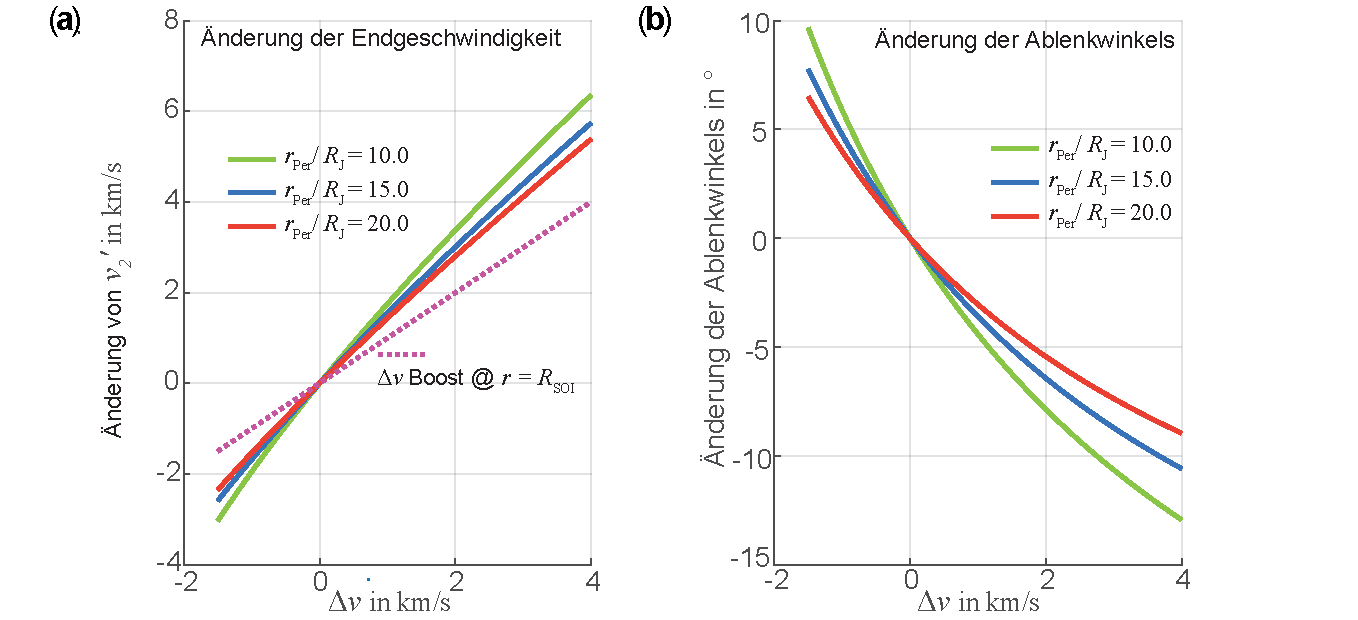
\includegraphics[width=\textwidth]{SwingByOberth01.pdf} 
	\caption[Geschwindigkeits- und Richtungs�nderung beim Gravity-Assist-Man�ver mit zus�tzlichem Schub.]{\fa Geschwindigkeits- und \fb Richtungs�nderung beim Gravity-Assist-Man�ver mit zus�tzlichem Schub am Beispiel Swing-By Jupiter. Man erkennt deutlich, dass der Geschwindigkeitszuwachs, wenn der Boost am Perizentrum erfolgt, deutlich gr��er ist als wenn dieser beim Eintreffen in die SOI des Jupiters erfolgen w�rde. Parameter siehe \mscr~ \mladynref{OberthSwingBy.m}.}
	\label{abb:adyn_swby03}
\end{figure}

\end{sol} 
\textcolor{blue} {$\rightarrow$ zur} \probref{adyn_swingby04}.\\
\noindent\rule[1ex]{\textwidth}{0.5pt} \newpage  \clearpage

%---------------------------------------------------------------------------------------------------


\begin{sol}{prob:adyn_raumfahrtschrott}\label{lsg:adyn_raumfahrtschrott} %Zusatz
\textbf{Raumfahrtschrott}\\

\begin{enumerate}
	\item\textit{\textbf{``Lebensdauer'' von Weltraumm�ll}}\\
	
Die Verweildauer von Weltraumm�ll in einer niedrigen Erdumlaufbahn
(\textit{Low Earth Orbi}t, LEO) wird im Wesentlichen durch den
atmosph�rischen Widerstand bestimmt.
Eine eindeutige Zuordnung \emph{Bahnh�he \(\to\) Lebensdauer} ist nicht
m�glich, da die Lebensdauer stark von
\begin{itemize}
  \item dem \emph{ballistischen Koeffizienten} \(A/m\) (projizierte Fl�che pro Masse),
  \item dem Aerodynamik-Koeffizienten \(C_\text{D}\),
  \item der zeitlich variablen Atmosph�rendichte \(\varrho(h,t)\) (stark variierend mit der Sonnenaktivit�t)
\end{itemize}
abh�ngt. Dennoch lassen sich f�r typische Objekte im All sinnvolle
Absch�tzungen angeben.

F�r ein Objekt der Masse \(m\) und Fl�che \(A\)
sei der aerodynamische Widerstand in erster N�herung (siehe Band I)
\begin{equation}
a_\text{drag}
= \frac{1}{2}\,\varrho(h)\,\,v^2\,C_\text{D}\,\frac{A}{m},
\end{equation}
wobei \(\varrho(h)\) die Atmosph�rendichte in H�he \(h\) und
\(v\) die Bahngeschwindigkeit ist.
Der Faktor \(C_\text{D} A/m\) wird h�ufig durch den
\emph{ballistischen Koeffizienten} charakterisiert:
\begin{equation}
B = \frac{m}{C_\text{D} A}
\quad\Leftrightarrow\quad
C_\text{D}\frac{A}{m} = \frac{1}{B}.
\end{equation}
Typische Werte f�r kleine Satelliten und gr��ere Tr�mmerobjekte liegen im Bereich
\begin{equation}
\frac{A}{m} \sim 10^{-2}\,\si{\meter^2\per\kilo\gram},
\end{equation}
also z.\,B.\ \(A=\SI{10}{\meter^2}\),~\(m=\SI{1000}{\kilo\gram}\)
bei \(C_\text{D} \approx 2.2\).\\


Wir benutzen das exponentielles Atmosph�renmodell (siehe \kap{adyn_drag}).
In guter N�herung kann man die Atmosph�rendichte im LEO
durch ein Exponentialgesetz beschreiben:
\begin{equation}
\varrho(h)
= \varrho_\mathrm{ref}\,\exp\!\left(-\frac{h-h_\mathrm{ref}}{H}\right),
\label{eq:rhoexp}
\end{equation}
wobei \(\varrho_\mathrm{ref}\) eine Referenzdichte bei H�he \(h_\mathrm{ref}\)
und \(H\) eine feste Skalenh�he ist. In einem verbesserten Modell ist \(H\) h�hen- und
zeitabh�ngig und \(\varrho(h,t)\) h�ngt wie erw�hnt stark von der Sonnenaktivit�t ab;
Gleichung~\eqref{eq:rhoexp} ist daher nur ein sehr einfaches Modell.

F�r die Dynamik im Orbit betrachten wir eine einfache Kreisbahn mit Bahnradius $a = R_\text{\earth} + h$, wobei $R_\text{\earth}$ der Erdradius ist.
Die Bahnenergie pro Masse lautet
\begin{equation}
\varepsilon = -\frac{\mu}{2a}
\end{equation}
mit dem Standardgravitationsparameter \(\mu = GM_\text{\earth}\), wobei $M_\text{\earth}$ die Masse der Erde ist.

Durch den Drag wird Energie dissipiert. Die �nderungsrate der
Energie ist $\D \varepsilon /\D t = \mathbf{a}_\text{D}\cdot\mathbf{v} = - a_\text{D}\,v$, da der Widerstand entgegengesetzt zur Geschwindigkeit wirkt.
Andererseits gilt
\begin{equation}
\frac{\mathrm d\varepsilon}{\mathrm d t}
= \frac{\mathrm d}{\mathrm d t}\left(-\frac{\mu}{2a}\right)
= \frac{\mu}{2a^2}\,\frac{\mathrm d a}{\mathrm d t}.
\end{equation}
Damit folgt
\begin{equation}
\frac{\mu}{2a^2}\,\frac{\mathrm d a}{\mathrm d t}
= - a_\text{D}\,v.
\end{equation}
F�r eine Kreisbahn ist $v = \sqrt{\mu/a}$.
Setzt man den Ausdruck f�r \(a_\text{D}\) ein,
\begin{equation}
a_\text{drag}
= \frac{1}{2}\,\varrho(h)\,v^2\,C_\text{D}\,\frac{A}{m},
\end{equation}
so erh�lt man
\begin{equation}
\frac{\mu}{2a^2}\,\frac{\mathrm d a}{\mathrm d t}
= - \frac{1}{2}\,\varrho(h)\,v^3\,C_\text{D}\,\frac{A}{m}.
\end{equation}
Einsetzen von \(v^3 = \left(\mu/a\right)^{3/2}\) liefert
\begin{equation}
\frac{\mathrm d a}{\mathrm d t}
= - \varrho(h)\,C_\text{D}\,\frac{A}{m}\,\sqrt{\mu}\,\sqrt{a}.
\label{eq:adot}
\end{equation}
Da \(h = a - R_\text{\earth}\) ist, h�ngt \(\varrho\) �ber \eqref{eq:rhoexp}
implizit von \(a\) ab. Gleichung~\eqref{eq:adot} l�sst sich numerisch integrieren. Aus einer Starth�he \(h_0\) berechnet man die Zeit bis zu einer
Reentry-H�he \(h_\text{reentry}\) (\zb \SI{122}{\kilo\meter}).\\

Als Gr��enordnungen der Lebensdauer erhalten wir mit 
einem typischen ballistischen Koeffizienten
\(A/m\sim 10^{-2}\,\si{\meter^2\per\kilo\gram}\) und
des erq�hnten groben Modells der Erd-Atmosph�re folgende Werte:

\begin{itemize}
  \item \(h_0 \approx \SI{300}{\kilo\meter}\):
        Lebensdauer von Monaten bis \ca \(\SI{1}{Jahr}\).
  \item \(h_0 \approx \SI{400}{\kilo\meter}\):
        typische Lebensdauer einiger Jahre (\zb~\ca 3-5~ Jahre).
  \item \(h_0 \approx \SI{500}{\kilo\meter}\): \ca 10-20~Jahre.
  \item \(h_0 \approx \SI{600}{\kilo\meter}\): mehrere Jahrzehnte.
  \item \(h_0 \approx \SI{800}{\kilo\meter}\): Jahrhunderte, da die Atmosph�rendichte sehr gering ist.
  \item \(h_0 \gtrsim \SI{1000}{\kilo\meter}\): Jahrhunderte bis Jahrtausende; der atmosph�rischer Drag ist vernachl�ssigbar.
\end{itemize}

Diese Zahlen sind nur Gr��enordnungen. �nderungen der
Sonnenaktivit�t oder des ballistischen Koeffizienten k�nnen die
Lebensdauer leicht um Faktoren von \(2{-}10\) verschieben. 
%Sie entsprechen in etwa der Aussage in \cite{Krag2025}. Wir verweisen f�r Details auf \mscr{} \mladynref{Raumfahrtschrott.m}.\\
%F�r eine quantitative Beispielrechnung l�sst sich 
%Gleichung~\eqref{eq:adot} in Verbindung mit dem
%Exponentialmodell \eqref{eq:rhoexp} numerisch integrieren.
%Setzt man z.\,B.
%\begin{align*}
%\varrho_\mathrm{ref} &\sim 4\times10^{-12}\,\si{\kilo\gram\per\meter^3}
%\quad\text{bei}\quad h_\mathrm{ref} \approx \SI{400}{\kilo\meter},\\
%H &\sim \SI{60}{\kilo\meter},\\
%C_\text{D} &\approx 2{,}2,\qquad \frac{A}{m}\sim 10^{-2}\,\si{\meter^2\per\kilo\gram},
%\end{align*}
%so erh�lt man eine Kurve \(\,T(h_0)\,\) (Lebensdauer als Funktion der
%Starth�he), die qualitativ den oben genannten Gr��enordnungen entspricht.
%Eine Darstellung in doppelt-logarithmischer Form (logarithmische
%Skalierung in der Zeitachse) zeigt, dass die Lebensdauer mit der H�he
%sehr stark anw�chst.\\
%
%Zusammenfassen kann man sagen, das es keinen exakten Zusammenhang zwischen
%Bahnh�he und Lebensdauer gibt; der ballistische Koeffizient \(A/m\), der Widerstandsbeiwert \(C_\text{D}\) und die
%Sonnenaktivit�t spielen eine zentrale Rolle. In einer einfachen Absch�tzung erh�lt man 
%mit der Exponentialatmosph�re und typischen ballistischen Koeffizienten f�r die Verweildauer
%Gr��enordnungen von Jahren bei \(\sim\SI{400}{\kilo\meter}\) \bzw Jahrtausende bei \(\gtrsim\SI{1000}{\kilo\meter}\).

\item\textit{\textbf{Beseitigung von Weltraumm�ll mit Lasern}}\\
	
Wir betrachten nun ein ideales, kugelf�rmiges St�ck Weltraumm�ll
mit Durchmesser \(\SI{10}{\centi\meter}\) in einer kreisf�rmigen Bahn
in \(\SI{800}{\kilo\meter}\) H�he �ber der Erdoberfl�che.
Ziel ist es, durch Laserablation die Bahn so zu �ndern, dass
das Perig�um auf etwa \(\SI{300}{\kilo\meter}\) abgesenkt wird.
In dieser H�he ist der atmosph�rische Widerstand gro� genug,
dass das Objekt typischerweise innerhalb von deutlich weniger als 5 Jahren 
wieder in die Atmosph�re eintritt (genaue Lebensdauer
h�ngt vom Atmosph�renmodell und dem ballistischen Koeffizienten ab) und vergl�ht.

Wir wollen eine grobe Absch�tzung der erforderlichen Laserenergie
f�r die Verwendung von Laserablation zur Weltraumm�ll-Beseitigung machen.

\subparagraph{Orbitdynamik}

Wir modellieren die Erde mit Radius $R_\text{\earth} \approx \SI{6371e3}{\meter}$
und Standardgravitationsparameter
$\mu_\text{\earth} \approx \SI{3.986e14}{\meter^3\per\second^2}$.
Die Ausgangsbahn sei kreisf�rmig mit H�he $h_0 = \SI{800e3}{\meter}$, und damit $r_0 = R_\text{\earth} + h_0$.
Die Kreisbahngeschwindigkeit ist
\begin{equation}
v_{\text{K,0}}
= \sqrt{\frac{\mu_\text{\earth}}{r_0}}.
\end{equation}
Als Zielbahn soll eine elliptische Bahn mit Apog�um in \(\SI{800}{\kilo\meter}\)
und Perig�um in \(\SI{300}{\kilo\meter}\) angenommen werden:
\[
h_\text{P} = \SI{300e3}{\meter},\quad
r_\text{P} = R_\text{\earth} + h_\text{P},\quad
r_\text{A} = r_0.
\]
Die gro�e Halbachse dieser lautet dann $a = (r_\text{P} + r_\text{A})/2$.
Die Geschwindigkeit im Apog�um dieser elliptischen Bahn ergibt sich
aus der \textit{vis-viva-Gleichung}\index{vis-viva-Gleichung} \eqref{eq:hm_vis-viva}:
\begin{equation}
v_\text{A}
= \sqrt{\mu_\text{\earth}\left(\frac{2}{r_\text{A}} - \frac{1}{a}\right)}.
\end{equation}
Wir brauchen  also am Apog�um eine retrograde Geschwindigkeits�nderung \(\Delta v\), um von der
kreisf�rmigen in die elliptische Bahn zu wechseln:
\begin{equation}
\Delta v = v_{\text{K,0}} - v_\text{A}.
\end{equation}
Mit den Zahlenwerten erhalten wir
%\begin{align}
%r_0 &= R_\text{earth} + \SI{800e3}{\meter},\\
%r_\text{P} &= R_\text{earth} + \SI{300e3}{\meter},\\
%a &= \frac{r_0 + r_\text{p}}{2}.
%\end{align}
%Damit erh�lt man numerisch
$ v_{\text{c,0}} \approx \SI{7456}{\meter\per\second},\,\,v_\text{A} \approx \SI{7320}{\meter\per\second},\,\, \Delta v \approx \SI{136}{\meter\per\second}$.
Dieses \(\Delta v\) gen�gt, um das Perig�um auf \ca \(\SI{300}{\kilo\meter}\)
abzusenken. 
%Noch niedrigere Zielh�hen (z.\,B. \(\SI{200}{\kilo\meter}\))
%w�rden ein etwas gr��eres \(\Delta v\) erfordern (Gr��enordnung
%\(\sim \SI{160}{\meter\per\second}\)).\\

Wir nehmen an, dass das Objekt eine Kugel aus Aluminium
mit Durchmesser \(d = 2r = \SI{10}{\centi\meter}\) ist.
%Das Volumen der Kugel ist
%\begin{equation}
%V = \frac{4}{3}\pi r^3.
%\end{equation}
Mit einer typischen Dichte f�r Aluminium von
\(\varrho \approx \SI{2700}{\kilo\gram\per\meter^3}\) ist die Masse
$m = \varrho V \approx \SI{1.4}{\kilo\gram}$.
%In der Realit�t kann die Masse je nach Geometrie und Material
%stark variieren; \(\SI{1}{\kilo\gram}\) bis einige \(\SI{}{kg}\) f�r
%\(\sim\SI{10}{\centi\meter}\)-Objekte ist jedoch plausibel als Gr��enordnung.\\

Der f�r die Bahn�nderung notwendige Impuls ist
\begin{equation}
I_\text{ges} = m\,\Delta v \approx \SI{1.9e2}{\newton\second} \,.
\end{equation}

\subparagraph{Laserablation und Impuls-Kopplungskoeffizient}

Bei Laserablation wird eine d�nne Oberfl�chenschicht verdampft
und bildet einen Plasmastrahl. Der R�cksto� liefert den gew�nschten
Impuls. Als praktische Kenngr��e wird h�ufig der
\emph{Impuls-Kopplungskoeffizient} \(C_m\) verwendet:
\begin{equation}
C_\text{abl} = \frac{\Delta I}{E_\text{Laser}},
\end{equation}
also Impuls pro eingestrahlter Laserenergie. Die Einheit ist
\(\si{\newton\second\per\joule}\).

Typische Werte f�r \(C_\text{abl}\) bei Nanosekundenimpulsen im
\(\SI{1}{\micro\meter}\)-Bereich und geeigneten Energiewerten
liegen in der Gr��enordnung
\[
C_\text{abl}\sim 10^{-4} \dots 10^{-3}\,\si{\newton\second\per\joule},
\]
je nach Material, Wellenl�nge, Pulsdauer und Energie.

Die erforderliche Laserenergie zur Erzeugung des Gesamtimpulses
\(I_\text{ges}\) ist $E_\text{Laser} = I_\text{ges}/C_\text{abl}$.
Mit \(I_\text{ges} \approx \SI{1.9e2}{\newton\second}\) und
\(C_\text{abl} \approx \SI{3e-4}{\newton\second\per\joule}\) ergibt sich
\begin{align}
E_\text{Laser}
&\approx \frac{\SI{1.9e2}{}}{\SI{3e-4}{}}\,\SI{}{\joule} \approx \SI{6.4e5}{\joule} \approx \SI{0.64}{\mega\joule}\,.
\end{align}

F�r andere plausible Werte von \(C_\text{abl}\) ergibt sich z.\,B.
\begin{align*}
C_\text{abl} &= \SI{1e-4}{\newton\second\per\joule}
&&\Rightarrow&
E_\text{Laser} &\approx \SI{1.9e6}{\joule}
\approx \SI{1.9}{\mega\joule},\\
C_\text{abl} &= \SI{1e-3}{\newton\second\per\joule}
&&\Rightarrow&
E_\text{Laser} &\approx \SI{1.9e5}{\joule}
\approx \SI{0.19}{\mega\joule}.
\end{align*}

Wir erhalten also eine grobe Bandbreite von $E_\text{Laser} \sim 0.2 \dots 2\,\si{\mega\joule} $ f�r ein \(\SI{10}{\centi\meter}\)-Objekt mit \(\sim\SI{1.4}{\kilo\gram}\)
Masse und \(\Delta v \sim \SI{136}{\meter\per\second}\).

Setzen wir \(E_\text{Laser} \approx \SI{0.64}{\mega\joule}\) an,
so entspricht dies $E\text{el} = E_\text{Laser}/\eta$, wobei \(\eta\) der Gesamtwirkungsgrad vom Stromnetz bis zum
Zielobjekt ist (Laser-Wirkungsgrad, Strahlf�hrung, atmosph�rische
Verluste etc.). Selbst bei einem eher optimistischen Gesamtwirkungsgrad
$\eta \sim 10\%$ ergibt sich
\begin{equation}
E_\text{el} \approx \SI{1.8}{\kilo\watt\hour}\,.
\end{equation}
Das ist energetisch durchaus handhabbar, zumal sich die Ablation
�ber viele einzelne Impulse und zahlreiche Uml�ufe verteilen kann.\\

In einem realistischen Szenario w�rde man das Objekt bei jedem
�berflug des Laserstandorts (bzw.\ des Laser-Satelliten)
f�r kurze Zeit im Fokus haben und pro Passage eine gewisse Anzahl
von Impulsen einbringen. Der Gesamtimpuls von \ca
\(\SI{200}{\newton\second}\) kann also auf viele hundert oder tausende
Impulse verteilt werden, etwa in der Gr��enordnung
\begin{equation}
\Delta I_\text{pro Impuls} \sim 10^{-2} \dots 10^{-1}\,\si{\newton\second},
\end{equation}
je nach Impulsenergie.\\

Die gemachte Absch�tzung enth�lt
mehrere idealisierende Annahmen:
\begin{itemize}
  \item Das Objekt ist eine homogene Aluminiumkugel; reale Tr�mmer
        haben komplexe Geometrie und Materialkombinationen.
  \item Der Impuls-Kopplungskoeffizient \(C_\text{abl}\) h�ngt stark von
        verschiedenen Parametern ab.
  \item Die Orbitdynamik ist idealisiert (keine St�rungen, kein zus�tzlicher aerodynamischer Drag
        w�hrend der Absenkphase).
\end{itemize}

Bei der Bahn�nderung von Weltraumm�ll durch Laserbestrahlung stellt sich die Frage, ob neben dem R�cksto� durch die Ablationsplasmawolke auch der reine Photonenimpuls des Laserstrahls ber�cksichtigt werden muss.\\
Im eigentlichen Ablationsregime ist der Photonenimpuls in der Regel gegen�ber dem Ablationsr�cksto� vernachl�ssigbar. Unterhalb der Ablationsschwelle kann er dagegen der f�hrende Effekt sein. Wir wollen das quantitativ absch�tzen:
Allgemein kann man mit einem dimensionslosen Kopplungsfaktor \(C_R\) der Impuls�bertrag  als (siehe Band V):
\begin{align}
	\Delta I_\text{photon} = C_\text{R} \frac{E_\text{Laser}}{c}\, \qquad 1 \le  C_\text{R}R \le 2
\end{align}
f�r den Bereich zwischen idealer Absorption und idealer Spiegelung schreiben.
Daraus folgt f�r den Impuls pro Joule bei Absorption
\[
\lk \frac{\Delta I_\text{photon}}{E_\text{Laser}}\rk_\gamma \approx \SI{3.33e-9}{\newton\second\per\joule}\,,
\]
und bei perfekter Reflexion maximal der doppelte Betrag, was sehr klein ist.
Das Verh�ltnis von Ablationsimpuls zu Photonenimpuls ist
\[
\frac{\Delta I_\text{abl}}{\Delta I_\text{photon}} = \frac{C_\text{abl} E_\text{Laser}}{C_\text{R} E_\text{Laser}/c} = \frac{C_\text{abl}}{C_\text{R}}c\,.
\]
Mit $C_\text{abl} = \SI{1e-5}{\newton\second\per\joule}$ erh�lt man f�r $\Delta I_\text{abl}/\Delta I_\text{photon}$ einen Wert von \ca $\SI{3e3}{}$.
Der Ablationsr�cksto� ist also typischerweise um drei bis vier Gr��enordnungen gr��er als der reine Photonenimpuls.\\

Trotz unserer gemachten Vereinfachungen liefert die Rechnung eine sinnvolle
Gr��enordnung: F�r ein \(\SI{10}{\centi\meter}\)-Objekt in \(\SI{800}{\kilo\meter}\)
H�he liegt die erforderliche Laserenergie zur Absenkung des Perig�ums
auf etwa \(\SI{300}{\kilo\meter}\) typischerweise im Bereich einiger
\(\SI{}{\mega\joule}\) auf dem Zielobjekt, was technisch prinzipiell
machbar ist, wenn man die Ablation �ber viele Uml�ufe verteilt. In Bezug auf reine Energiegr��enordnungen erscheint
ein Laser-basiertes Deorbiting einzelner \(\SI{10}{\centi\meter}\)-Objekte
prinzipiell realistisch. Die eigentlichen Herausforderungen liegen eher
in Strahlf�hrung, Zielverfolgung und Systemkomplexit�t.
Insbesondere haben wir in unseren Rechnungen unber�cksichtigt gelassen, wie die Laserenergie von der Erde so zum Tr�mmerobjekt gebracht werden kann, \dh ausgerichtet und fokussiert werden kann, dass die gesamte \bzw ein Gro�teil der von der Erde abgestrahlten Energie das relativ kleine Tr�mmerobjekt trifft. Mit solchen, im Wesentlichen optischen Fragen, wollen wir uns n�her im Band V besch�ftigen.  

%Nicht zuletzt soll erw�hnt werden, dass es f�r die Methode noch eine  Reihe rechtlicher und politischer Rahmenbedingungen zu kl�ren gilt.

%Zusammenfassung 
%
%\begin{itemize}
  %\item Ben�tigtes \(\Delta v\) zur Absenkung des Perig�ums von
        %\(\SI{800}{\kilo\meter}\) auf \(\SI{300}{\kilo\meter}\):
        %\(\Delta v \approx \SI{136}{\meter\per\second}\).
  %\item Masse eines idealisierten \(\SI{10}{\centi\meter}\)-Aluminiumfragments:
        %\(m \approx \SI{1.4}{\kilo\gram}\).
  %\item Gesamtimpulsbedarf:
        %\(I_\text{ges} \approx \SI{2e2}{\newton\second}\).
  %\item Bei typischen Werten f�r den Impuls-Kopplungskoeffizienten
        %\(C_m \sim 10^{-4} \dots 10^{-3}\,\si{\newton\second\per\joule}\)
        %ergibt sich eine ben�tigte Laserenergie auf dem Zielobjekt von
        %\[
        %E_\text{Laser} \sim 0{,}2 \dots 2\,\si{\mega\joule}.
        %\]
%\end{itemize}
%
\end{enumerate}

\end{sol} 
\textcolor{blue} {$\rightarrow$ zur} \probref{adyn_raumfahrtschrott}.\\
\noindent\rule[1ex]{\textwidth}{0.5pt} 

%---------------------------------------------------------------------------------------------------

\newpage
\begin{sol}{prob:adyn_proxima_centauri}\label{lsg:adyn_proxima_centauri} %Zusatz
\textbf{Starshot and Starlight}\\


Wir verweisen auf \cite{Umrigar2025} und danken den Autoren f�r dieses instruktive physikalische Problem.\\

\end{sol} 
\textcolor{blue} {$\rightarrow$ zur} \probref{adyn_proxima_centauri}.\\
\noindent\rule[1ex]{\textwidth}{0.5pt} 



%---------------------------------------------------------------------------------------------------

\newpage
\begin{sol}{prob:adyn_waterrocket}\label{lsg:adyn_waterrocket} %Zusatz
\textbf{Wasserrakete}\\

Gegeben sind folgende Parameter:
\begin{itemize}
  \item Wasservolumen $V_\text{W0}$, Luftvolumen �ber dem Wasser $V_\text{A0}$, Flaschenvolumen $V_\text{F}=V_\text{W0}+V_\text{A0}$.
  \item Druck der komprimierten Luft $p_0$ als Absolutdruck.
  \item D�sendurchmesser $d_\text{N}$ mit Querschnitt $A_\text{N}=\pi(d_\text{N}/2)^2$.
  \item Abschusswinkel $\theta$ (konstant als Schubrichtung angenommen).
  \item Trockenmasse $m_\mathrm{F}$ (Flasche+Nase+Finnen), aerodynamische Parameter $C_\text{D}$ und Referenzfl�che $A_\mathrm{ref}$.
\end{itemize}

Konstanten:
Wasserdichte $\varrho_\text{W}\approx 1000\,\mathrm{kg/m^3}$, Luftdichte $\varrho_\mathrm{A}\approx 1.2\,\mathrm{kg/m^3}$,
adiabatischer Exponent der Luft $\gamma\approx 1.4$,
Umgebungsdruck $p_\mathrm{Luft}\approx 101325\,\mathrm{Pa}$.
Der Ausflussbeiwert der D�se liege $C_\text{D,N}$ im Intervall $[0.8,0.95]$.

In der Wasser-Schubphase (Blowdown), \dh w�hrend Wasser ausstr�mt, vergr��ert sich das Luftvolumen $V_\text{A}(t)$, und der Flaschendruck f�llt adiabatisch:
\begin{equation}
p(t)=p_0\left(\frac{V_\text{A0}}{V_\text{A}(t)}\right)^\gamma.
\end{equation}
Der antreibende Differenzdruck ist $\Delta p(t)=\max(p(t)-p_\mathrm{L},0)$.

F�r die Strahlgeschwindigkeit (wir nehmen die Bernoulli-L�sung (siehe Band I) mit Ausflussbeiwert gilt
\begin{equation}
v_\text{ex}(t)=C_\text{D,N}\sqrt{\frac{2\,\Delta p(t)}{\varrho_\text{W}}}.
\end{equation}
Damit folgen Volumenstrom \bzw  Massenstrom des Wassers:
\begin{equation}
\dot V(t)=A_n v_\text{ex}(t), ~~ \rightarrow~~ \dot m_\text{W}(t)=\varrho_\text{W} A_\text{N} v_\text{ex}(t).
\end{equation}
Eine einfache Schubn�herung in der Wasserphase ist die Impulsbilanz
\begin{equation}
T(t)\approx \dot m_\text{W}(t)\, v_\text{ex}(t).
\end{equation}
Diese ist gerechtfertigt, da der zus�tzliche Druckterm $(p_\text{ex}-p_\mathrm{amb})A_n$ bei freiem Wasserstrahl meist klein gegen�ber $\dot m v_\text{ex}$ ist. 
Die Luftvolumen�nderung ist identisch mit dem abgeflossenen Wasservolumen:
\begin{equation}
\dot V_\text{A}(t)=\dot V(t)=A_n v_\text{ex}(t).
\end{equation}
Die Wasserphase endet bei $V_\text{A}(t)=V_\text{F}$ (Wasser ist leer) oder wenn $\Delta p(t)=0$.
Die Wassermasse ist $m_w(t)=\varrho_w V_\text{W}(t)$ und f�llt mit
\begin{equation}
\dot m_\text{W}(t)=-\varrho_\text{W} A_\text{N} v_\text{ex}(t).
\end{equation}
Die Gesamtmasse sei (w�hrend der Wasserphase)
\begin{equation}
m(t)=m_\mathrm{F}+m_\text{W}(t)+m_\mathrm{A},
\end{equation}
wobei $m_\mathrm{A}$  als konstant angenommen werden kann.

Der aerodynamischer Widerstand wird quadratisch angesetzt (wir haben nach einfacher Absch�tzung eine gro�e Reynolds-Zahl, die Turbulenz ergibt):
\begin{equation}
\mathbf{F}_\text{D}=\frac12\varrho_\mathrm{air} C_\text{D} A_\mathrm{ref} \, |\vec{v}|\,\vec{v}.
\end{equation}
Die Schubrichtung wird als konstant entlang des Abschusswinkels $\theta$ angenommen (Das setzt voraus, dass zumindest in der Schubphase die Rakete ihrer Abschussrichtung beibeh�lt,  genauer w�re eigentlich wenn Schubrichtung der Tangente an die Bahn entspricht.)
\begin{equation}
\vec{T}(t)=T(t)\begin{pmatrix}\cos\theta\\ \sin\theta\end{pmatrix}.
\end{equation}
Dann lautet die Bewegungsgleichung:
\begin{equation}
m(t)\, \dot{\mathbf{v}}=\vec{T}(t)-\vec{F}_\text{D} - m(t)\,g\begin{pmatrix}0\\1\end{pmatrix}.
\end{equation}
Die Numerische Integration erfolgt in Zeitschritten $\Delta t$ mit explizitem Euler-Verfahren oder der \matlab~\odevf-Rotine.
Ausgegeben werden die Trajektorien $(x(t),y(t))$, $(t,z(t))$, die maximale H�he $z_\mathrm{max}$, die Flugzeit $t_\mathrm{impact}$ und die Reichweite $x(t_\mathrm{impact})$ (bei $z=0$). Ergebnisse haben wir f�r die Werte unserer Modellraket (Tabelle \ref{tab:adyn_param_wasserrakete}) zeigen wir in \figref{adyn_WaterRocket}.\\
\begin{table}%tab1
\smallskip
\begin{tabular}{L{4cm}L{4cm}}
\svhline\noalign{\smallskip}
\noalign{\smallskip}
\textbf{Gr��e} & \textbf{Wert} \\
\noalign{\smallskip}\svhline\noalign{\smallskip}
Wasservolumen bei $t=0$ & $0.375\,\mathrm{l}$ \\
Luftvolumen bei $t=0$   & $0.375\,\mathrm{l}$ \\
Masse der Flasche       & $70.00\,\mathrm{g}$ \\
Druck bei $t=0$         & $650000.00\,\mathrm{Pa}$ \\
D�sendurchmesser        & $5.00\,\mathrm{mm}$ \\
$C_\text{D}$-Wert       & $0.40$ \\
Querschnitt             & $19.63\,\mathrm{cm^2}$ \\
Winkel                  & $55.00^\circ$ \\
\hline
Reichweite              & $86.1\,\mathrm{m}$ \\
Maximale H�he           & $33.7\,\mathrm{m}$ \\
Flugzeit                & $5.79\,\mathrm{s}$ \\
\noalign{\smallskip}
\svhline\noalign{\smallskip}
\end{tabular}
\caption{Parameter und Messwerte der Wasserrakete}
\label{tab:adyn_param_wasserrakete}
\end{table}
\begin{figure}
	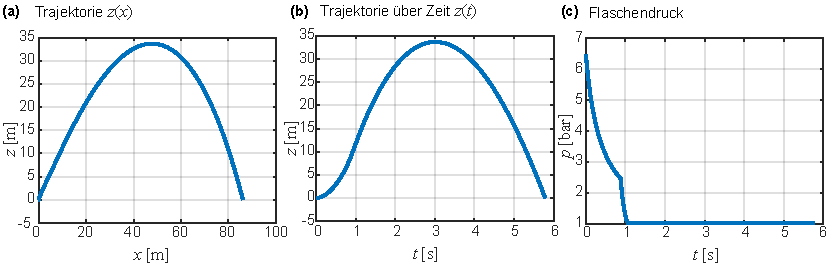
\includegraphics[scale=1]{WaterRocket.pdf} 
	\caption[Trajektorie einer Wasserrakete.]{Trajektorie einer Wasserrakete. Parameter siehe Tabelle \ref{tab:adyn_param_wasserrakete} und \mscr~ \mladynref{WaterRocket.m}.}
	\label{abb:adyn_WaterRocket}
\end{figure}

Bei der numerischen Integration m�ssen wir auf  einen ``stetigen'' �bergang zwischen Wasser- und Gasphase achten, denn im einfachen Modell wird beim Erreichen von $m_\text{W}=0$ abrupt von der Wasser-Schubformel auf die Gas-Schubformel umgeschaltet. Dadurch w�rde im Schub-Zeit-Diagramm unter Umst�nden 
eine unphysikalisch Diskontinuit�t auftreten. Zur numerischen Regularisierung verwenden wir deshalb eine kleine �bergangszone f�r sehr kleine Restwassermassen. Sei
$ m_{\text{W}0}=\varrho_\text{W} V_{\text{W}0}$ die Anfangswassermasse und $\varepsilon \ll 1$ ein kleiner Bruchteil, \zb $0.02$, dann wird f�r
$m_\text{W} \le \varepsilon\, m_{\text{W}0}$
ein ``glatter'' Mischfaktor
\begin{align}
	w = \frac12 \lek 1+\cos\!\lk \pi \lk 1-\frac{m_\text{W}}{\varepsilon m_{\text{W}0}}\rk \rk \rek
\end{align}
verwendet. Dann gilt:
\[
w=1 \quad \text{bei} \quad m_\text{W}=\varepsilon m_{\text{W}0}, \qquad w=0 \quad \text{bei} \quad m_\text{W}=0\,.
\]
Der Schub wird in dieser Zone als gewichtete Summe geschrieben:
$T = w\,T_\mathrm{W} + (1-w)\,T_\mathrm{A}$, Analog kann auch der Massenstrom gegl�ttet werden:
\[
\dot m = w\,\dot m\text{W} + (1-w)\,\dot m_\text{A}.
\]
Diese Vorgehensweise ist in erster Linie eine numerische Regularisierung und kein
vollst�ndiges physikalisches Zweiphasenmodell, f�hrt aber zu einer realistischen und numerisch stabilen
Schubkurve.\\

Die �bereinstimmung der numerischen Rechnung mit den Beobachtungen ist damit relativ gut, insbesondere wenn man die gemachten groben N�herungen ber�cksichtigt.\\

Wir wollen das Ganze jetzt noch mit einer so genannten Fehlerlandkarte (\textit{Error-Map}) �berpr�fen. Das Ziel ist, aus den experimentellen Messdaten Reichweite, maximale H�he, Flugzeit 
($R_{\mathrm{exp}}, H_{\mathrm{exp}}$ und $T_{\mathrm{exp}}$ )
die plausiblen unbekannten Modellparameter zu bestimmen. 
Im unserem Fall werden als freie Parameter der aerodynamische Widerstandsbeiwert  $C_\text{D}$ und der absolute Anfangsdruck $p_0$ genommen. 
Alle �brigen Gr��en, insbesondere die geometrischen Gr��en der Rakete, werden als bekannt angenommen.
Die Methode basiert auf einer systematischen Abtastung des Parameterraums und der Bewertung der jeweiligen Parameterkombination durch eine Fehlerfunktion.
Das physikalische Modell, im \mscr{}~ durch 
$\textcolor{mygreen}{\texttt{waterRocketSim}}$ 
realisiert, definiert eine Abbildung der Art
\begin{align}
	(C_\text{D}, p_0) ;\longmapsto; \lk R_{\mathrm{sim}}, H_{\mathrm{sim}}, T_{\mathrm{sim}}\rk \,.
\end{align}
Zum Vergleich zwischen Simulation und Messung werden relative Fehler definiert:
\begin{align*}
	e_R &= \frac{R_{\mathrm{sim}} - R_{\mathrm{exp}}}{R_{\mathrm{exp}}}\,,\quad e_H = \frac{H_{\mathrm{sim}} - H_{\mathrm{exp}}}{H_{\mathrm{exp}}}\,,\quad
	e_T = \frac{T_{\mathrm{sim}} - T_{\mathrm{exp}}}{T_{\mathrm{exp}}}\,.
\end{align*}
Diese Normierung hat den Vorteil der dimensionslosen Darstellung und der gleichen Gewichtung der Messwerte unabh�ngig von der Gr��enordnung.

\begin{figure}
	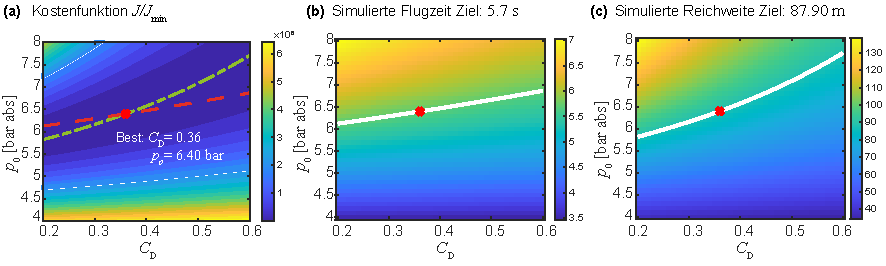
\includegraphics[scale=1]{WaterRocket02.pdf} 
	\caption[Error-Map einer Wasserrakete f�r die Variablen Parameter $p_0$ und $C_\text{D}$.]{Error-Map einer Wasserrakete f�r die variablen Parameter $p_0$ und $C_\text{D}$. \fa Error-Map mit Schnittpunkt Flugzeit und Reichweite als Messwerte der Wasserrakete \fb Zielsimulation auf die Messwert Flugzeit der Wasserrakete, \fc Zielsimulation auf die Messwert Reichweite der Wasserrakete. Parameter siehe Tabelle \ref{tab:adyn_param_wasserrakete} und \mscr~ \mladynref{WaterRocket.m}.}
	\label{abb:adyn_WaterRocket02}
\end{figure}

Die Fehler werden zu einer skalaren Kostenfunktion kombiniert:
\begin{align}
	J(C_\text{D},p_0) = w_R e_R^2 + w_H e_H^2 + w_T e_T^2\,~~\text{mit Gewichtungsfaktoren}~~w_R, ~ w_H, ~ w_T \ge 0\,.
\end{align}
$J=0$ entspricht perfekter �bereinstimmung, kleine Werte von $J$ bedeuten gute Anpassung.
Der Parameterraum wird auf einem Gitter diskretisiert, woraus sich ein zweidimensionales Raster
$[C_{\text{D},i}, p_{0,j}] $ f�r $i=1,\dots,N,~ j=1,\dots,M$ ergibt.
F�r jedes Gitterelement wird die Simulation durchgef�hrt und aus den relativen Fehlern $e_R, e_H, e_T$ die Kostenfunktion ausgewertet:
Aus der erhaltenen Matrix ergibt sich der beste Parametersatz durch Minimierung.
In der Error-Map wird die Funktion $J(C_\text{D},p_0)$ \zb durch eine Farbkarte (\textit{Heatmap}) dargestellt.
Zus�tzlich werden h�ufig geplottet $R_{\mathrm{sim}}(C_\text{D},p_0)$, $T_{\mathrm{sim}}(C_\text{D},p_0)$ und $H_{\mathrm{sim}}(C_\text{D},p_0)$.
Besonders aussagekr�ftig sind die Konturen $R_{\mathrm{sim}} = R_{\mathrm{exp}}$, $T_{\mathrm{sim}} = T_{\mathrm{exp}}$ und $H_{\mathrm{sim}} = H_{\mathrm{exp}}$.
Schnittpunkte dieser Kurven im Parameterraum entsprechen konsistenten L�sungen, mehrere Schnittpunkte bedeuten Nicht-Eindeutigkeit und  keine Schnittpunkte deuten auf Modellabweichungen hin.\\

Die Error-Map ist ein zentrales Werkzeug zur Modellvalidierung und Parameteridentifikation und liefert eine hilfreiche diskrete Approximation der Funktion $J(C_\text{D},p_0)$ dar, welche den Abstand zwischen Simulation und Experiment misst.
Sie erlaubt eine visuelle Analyse des Parameterraums, eine Bestimmung optimaler Parameter und die Identifikation von Unsicherheiten und Korrelationen.\\

\subparagraph{Modellverfeinerungen und zus�tzliche Problemstellungen:}

In einer Verfeinerung des Modells k�nnte man ber�cksichtigen:
\begin{enumerate} [1)]
	\item die Beschreibung der Rakete als starren K�rper mit ver�nderlichen Schwerpunkt, 
	\item den Pitch (Nickbewegung) der Richtung des Schubs durch die Wirkung Schwerkraft/Reibung auf die Rakete,
	\item den Auftrieb der Rakete und
	\item die Rotation der Rakete um die L�ngsachse (hervorgerufen durch die seitlichen ``Flossen'').
\end{enumerate}

Eine weitere sch�ne �bung ist der Vergleich mit der Trajektorie eines schr�gen Wurfs, der die gleiche H�he und Reichweite erreicht. 
Man vergleiche insbesondere die dazu notwendige  Abwurfgeschwindigkeit. (Wir verweisen auch auf die �bung 1.41 in Band I Mechanik).
Wir finden interessanterweise, dass man bei einer Abwurfgeschwindigkeit von udn einem Abwurfwinkel eine Trajektorie $z(x)$ erh�lt, die in etwa mit der Trajektorie der Wasserrakete �bereinstimmt und zwar sowohl bei Scheitelh�he als auch Reichweite.
Das Zeitverhalten ist aber leicht unterschiedlich (die Rakete muss ja erst beschleunigt werden), so dass der Wurf eine um 0.5 s verk�rzte Flugzeit hat. Siehe dazu die \mscr{}e \mladynref{WaterRocket.m} und \mladynref{WaterRocketVergleichWurf.m}.

%Wir wollen die Punkte 1) bis 3) gemeinsam angehen und die Rakete nicht mehr als Punktmasse behandeln, sondern als starren K�rper (in der $x$-$z$-Ebene).
%Dadurch k�nnen zus�tzlich zur translatorischen Bewegung auch die Orientierung und die Nickbewegung beschrieben werden.
%
%Das Modell umfasst:
%\begin{itemize}
%\item Translation des Schwerpunkts in der Ebene $(x,z)$,
%\item Rotation der Rakete mit Winkel $\theta$,
%\item Winkelgeschwindigkeit $\omega=\dot\theta$,
%\item zeitabh�ngige Gesamtmasse $m(t)$,
%\item zeitabh�ngigen Schwerpunkt $x_{CG}(t)$ entlang der Raketenachse,
%\item zeitabh�ngiges Tr�gheitsmoment $I_{CG}(t)$.
%\end{itemize}
%
%Der Zustandsvektor sei
%\[
%\vec{Y}(t)= \lek x, z, v_x, v_z, \theta, \omega, m_\text{W},  m_\text{A} \rek^\text{T}\,.
%\]
%Dabei ist $\theta$ die Orientierung der Raketenachse gegen die $x$-Achse und ,
%$\omega$ die Nickrate. Die anderen Parameter wurden bereits oben eingef�hrt.
%Die Raketenachse ist durch den Einheitsvektor
%\[
%\vec e_\text{R}=
%\begin{pmatrix}
%\cos\theta\\
%\sin\theta
%\end{pmatrix}
%\]
%gegeben.
%Ein dazu senkrechter Einheitsvektor ist
%\[
%\vec e_n=
%\begin{pmatrix}
%-\sin\theta\\
%\cos\theta
%\end{pmatrix}.
%\]
%Die Geschwindigkeit des Schwerpunkts ist
%\[
%\vec v=
%\begin{pmatrix}
%v_x\\
%v_z
%\end{pmatrix},
%\qquad
%V=\|\mathbf v\|=\sqrt{v_x^2+v_z^2}.
%\]
%Der Flugbahnwinkel (siehe \kap{}) ist $\gamma=\operatorname{atan2}(v_y,v_z)$.
%Der Anstellwinkel (ebenfalls Verweis auf\kap{}) der Rakete relativ zur Flugrichtung wird definiert als $\alpha=\theta-\gamma$.
%F�r kleine Winkel ist $\alpha$ der zentrale aerodynamische P
%%Die Gesamtmasse ist
%%\[
%%m(t)=m_{\mathrm{F}} + m_\text{W}(t) + m_\text{W}(t) + m_a(t).
%%\]a(t).
%%\]
%%
%Die Lage des Schwerpunkts entlang der Raketenachse werde durch $x_\text{S}(t)$
%beschrieben. Sie kann aus den Teilmassen berechnet werden:
%\[
%x_\text{S}(t)=\frac{\sum_i m_i(t)x_i}{\sum_i m_i(t)},
%\]
%wobei man typischerweise die Rakete in die Bestandteile trockene Flasche, Wasserf�llung, Luft, Nase und Flossen zerlegt.
%Das Tr�gheitsmoment um den Schwerpunkt ist
%\[
%J_\text{S}(t)=\sum_i \lk J_i^{(\mathrm{eig})} + m_i(t) \lek (x_i-x_\text{S}(t)\rek^2\rk\,.
%\]
%Es wirken im Wesentlichen vier Kr�fte:
%\begin{enumerate} [(a)]
	%\item Schwerkraft\\
			%\[
		%\mathbf F_g=
		%\begin{pmatrix}
		%0\\
		%-\,m(t)g 
		%\end{pmatrix}.\]
	%\item Schub\\
	%Der Schub wirkt entlang der Raketenachse: $\mathbf F_T = T(t)\,\vec e_\text{R}$.
	%\item Luftwiderstand\\
	%Der Widerstand wirkt entgegen der Flugrichtung:
		%\[
		%\mathbf F_D
		%=
		%-\frac12 \rho_{\mathrm{air}} V^2 A_{\mathrm{ref}} C_\text{D} \,\vec e_v,
		%\]
		%wobei $\mathbf e_v=\frac{\mathbf v}{V}$ f�r $V>0$.
	%\item Normalkraft\\
		%Die aerodynamische Normalkraft wird f�r kleine Anstellwinkel modelliert durch $N=\frac12 \rho_{\mathrm{A}} V^2 A_{\mathrm{ref}}\, C_{N\alpha}\,\alpha$. Sie wirkt senkrecht zur Raketenachse, \dh $\vec{F}_N = N\,\vec{e}_n$.
%\end{enumerate}
%
%Die Translation des Schwerpunkts folgt der Newton-Bewegungsgleichung. 
%\begin{align}
	%m(t)\,\dot{\mathbf v} &= \mathbf F_T + \mathbf F_D + \mathbf F_N + \mathbf F_g\,\\
%\end{align}
%\bzw in Komponentenschreibweise:
%\begin{align}
%\begin{split}
	%\dot x   &= v_x\,,\\
	%\dot z 	 &= v_z\,,\\
	%\dot v_x &= \frac{F_{T,x}+F_{D,x}+F_{N,x}}{m(t)}\,,\\
	%\dot v_z &= \frac{F_{T,y}+F_{D,y}+F_{N,y}}{m(t)} - g\,.
%\end{split}
%\end{align}
%Die Rotationsgleichung um den Schwerpunkt lautet
%\begin{align}
	%I_\text{S}(t)\,\dot\omega = M(t)~~~\text{mit}~~~\dot\theta=\omega\,.
%\end{align}
%Das dominierende Drehmoment ist h�ufig das aerodynamische Nickmoment $M_N = N\,(x_\text{CP}-x_\text{S})$, wobei $x_\text{CP}$ die Lage des Druckpunkts entlang der Raketenachse beschreibt. Zus�tzlich kann ein Schubmoment auftreten, wenn die Schublinie nicht exakt durch den Schwerpunkt geht, \dh $M_T = T\,\Delta_\perp$, mit seitlichem Hebelarm $\Delta_\perp$.
%Damit haben wir insgesamt ein Drehmoment von:
%\[
%M = M_N + M_T + M_{\mathrm{d}}\,,
%\]
%wobei f�r das aerodynamische D�mpfungsmoment $M_{\mathrm{d}} = -C_q\,\omega$ eingesetzt werden kann oder besser noch
%\[
%M_{\mathrm{d}} = -\frac12 \rho_{\mathrm{A}} V^2 A_{\mathrm{ref}} L_{\mathrm{ref}}^2 C_{m_q}\,\omega\,.
%\]
%Die innere Antriebsdynamik kann aus dem einfachen Massenpunkt-Modell �bernommen werden.\\
%Damit lauten die Bewegungsgleichungen f�r das Gesamtsystem (2D-System eines Starren K�rpers):
%\begin{subequations}
%\begin{align}
	%\dot x &= v_x,\\
	%\dot z &= v_z,\\
	%\dot v_x &= \frac{F_{T,x}+F_{D,x}+F_{N,x}}{m},\\
	%\dot v_z &= \frac{F_{T,y}+F_{D,y}+F_{N,y}}{m} - g,\\
	%\dot\theta &= \omega,\\
	%\dot\omega &= \frac{M_N + M_T + M_{\mathrm{d}}}{J_\text{S}},\\
	%\dot m_\text{W} &= \text{aus Blowdown-Phase Massenpunkt-Modell},\\
	%\dot m_\text{A} &= \text{aus Gas-Phase Massenpunkt-Modell}\,.
%\end{align}
%\end{subequations}
%Dieses Modell erlaubt:
%\begin{itemize}
	%\item Unterschied zwischen Raketenachse und Flugbahnrichtung,
	%\item dynamische �nderung des Anstellwinkels,
	%\item Stabilit�tsanalyse �ber den Abstand $x_\text{CP}-x_\text{S}$,
	%\item Einfluss der Schwerpunktwanderung w�hrend der Wasserentleerung,
	%\item realistischere Beschreibung von Pitch und Bahnkr�mmung.
%\end{itemize}

\end{sol} 
\textcolor{blue} {$\rightarrow$ zur} \probref{adyn_waterrocket}\\
\noindent\rule[1ex]{\textwidth}{0.5pt} 


 
%\clearpage
%\section{L�sungsbeispiele Kapitel \ref{chap:kontmech} -- Physik des Kontinuums}\label{chap:kontmech_lsguebungen}

Die in den L�sungsvorschl�gen angegebenen \mscre finden sich im GitHub unter \githubSN \bzw
in den \onlineZ{} (\MKc).\\
Sie sind wirklich als Vorschlag f�r eine m�gliche L�sung gedacht, wohl wissend, dass es in der Physik oft ganz verschiedene, manchmal auch elegantere als die hier vorgestellten L�sungen gibt, um ein Problem zu l�sen. Das macht ja gerade den Reiz der Physik aus.
Wir laden die Leser ein, ihre L�sungen auch unter \githubSN \bzw auf den online-Seiten (\MKc) zu teilen.
Wir sind in jedem Fall gespannt.

%-----------------------------------------------------------------------------------------------------------

\subsection{�bungen zu Bewegungen von Fl�ssigkeiten und Gasen}

\medskip

%-----------------------------------------------------------------------------------------------------------

\begin{sol}{prob:kontmech_diffoperators}\label{lsg:kontmech_diffoperators} %�bung1
\textbf{Differentialoperatoren}
\begin{enumerate}
    \item [1.]
    \begin{enumerate}
        \item [a)]
        \begin{align}
            \Phi \lk \vec{r}\rk &= x\,y\,\e^{-r^2} ~~\rightarrow~~~ \gradv\,\Phi = \begin{pmatrix}
                y-2x^2\,y\\
                x-2x\,y^2\\
                -x\,y\,z
            \end{pmatrix}\,
            \e^{-r^2} \,. \label{eq:kontmech_Ueb1_01}
        \end{align}
        \item[b)]
        \begin{align}
        \begin{split}
             \Phi \lk\vec{r}\rk &= C\,\frac{\e^{-\alpha\,r}}{r} ~~\rightarrow~~~ \gradv\,\Phi =C\,\begin{pmatrix}
                x\,\lk 1+\alpha\,r\rk\\
                y\,\lk 1+\alpha\,r\rk\\
                z\,\lk 1+\alpha\,r\rk\\
            \end{pmatrix}\,
            \frac{\e^{-\alpha\,r}}{r^3}  \\
            &=
            \begin{pmatrix}
                x\\
                y\\
                z
            \end{pmatrix} \,C\,\frac{\lk 1+\alpha\,r\rk}{r^3}\,e^{-\alpha\,r} = C\,\vec{r}\,\frac{1+\alpha\,r}{r^3}\,\e^{-\alpha\,r} 
        \end{split} \,. \label{eq:kontmech_Ueb1_02}
        \end{align}
        Alternativ berechnen wir direkt in sph�rischen Koordinaten, da $\varphi$ nicht von den $\phi$ und $\theta$ abh�ngt, ist der Gradient einfach:
        \begin{align}
        \begin{split}
            \gradv\,\Phi &= \frac{\d\Phi}{\d r}\,\vec{e}_r =\frac{\d\Phi}{\d r}\,\frac{\vec{r}}{r}\\
            \frac{\d \Phi}{\d r}&= C\,\frac{\lk 1+\alpha\,r\rk}{r^2}\,\e^{-\alpha\,r}~~\rightarrow~~~\gradv\,\,\Phi = C\,\vec{r}\,\frac{\lk 1+\alpha\,r\rk}{r^3}\,\e^{-\alpha\,r}
        \end{split}  \,. \label{eq:kontmech_Ueb1_03} 
        \end{align}
    \end{enumerate}
    \item [2)]
    \begin{enumerate}
        \item [a)]
        \begin{align*}
            \divv\,\begin{pmatrix}
                x-z\\
                x\,z\\
                y^2
            \end{pmatrix}
            = 1+0+0 =1  \,. 
        \end{align*}
        \item [b)]
        \begin{align*}
            \divv\,
            \begin{pmatrix}
                5x^2\\
                3y^2\\
                0
            \end{pmatrix} =
            10x+6y+0 = 10x+6y  \,. 
        \end{align*}
    \end{enumerate}
    \item[3)]
    \begin{enumerate}
        \item [a)]
        \begin{align*}
            \rotv\,0.5\,\begin{pmatrix}
                y\,z^2\\
                -x\,z^2\\
                0
            \end{pmatrix} &= \rotv\,0.5\,
            \begin{pmatrix}
                f_1\\
                f_2\\
                f_3
            \end{pmatrix} =
             0.5\,
            \begin{pmatrix}
                \frac{\d f_3}{\d y} -\frac{\d f_2}{\d z} \\
                \frac{\d f_1}{\d z} -\frac{\d f_3}{\d x} \\
                \frac{\d f_2}{\d x} -\frac{\d f_1}{\d y}
            \end{pmatrix}
            = 0.5\,
            \begin{pmatrix}
                2x\,z\\
                2y\,z\\
                -2z^2
            \end{pmatrix}
            =
            \begin{pmatrix}
                x\,z\\
                y\,z\\
                z^2
            \end{pmatrix}  \,. 
        \end{align*}
        \item [b)]
        \begin{align*}
            \rotv\,
            \begin{pmatrix}
                0\\
                2x\,z + 3y^2\\
                4y\,z^2
            \end{pmatrix} 
            =
            \begin{pmatrix}
                -2x + 4z^2\\
                0\\
                2z
            \end{pmatrix}  \,. 
        \end{align*}
    \end{enumerate}
\end{enumerate}
Die Rechnungen finden sich im Detail im \mlkontmechref{VektorAnalysis01.m}. \\

Die graphischen Darstellungen zu den Differentialoperatoren finden sich in den \mscr en \mlkontmechref{GradientFunktion1.m},\mlkontmechref{GradientFunktion2.m},\mlkontmechref{GradientFunktion3.m}, \mlkontmechref{Divergenz.m} und \mlkontmechref{Rotation.m}. Einige Beispiele sind in den folgenden Bildern gezeigt.

\begin{figure}
    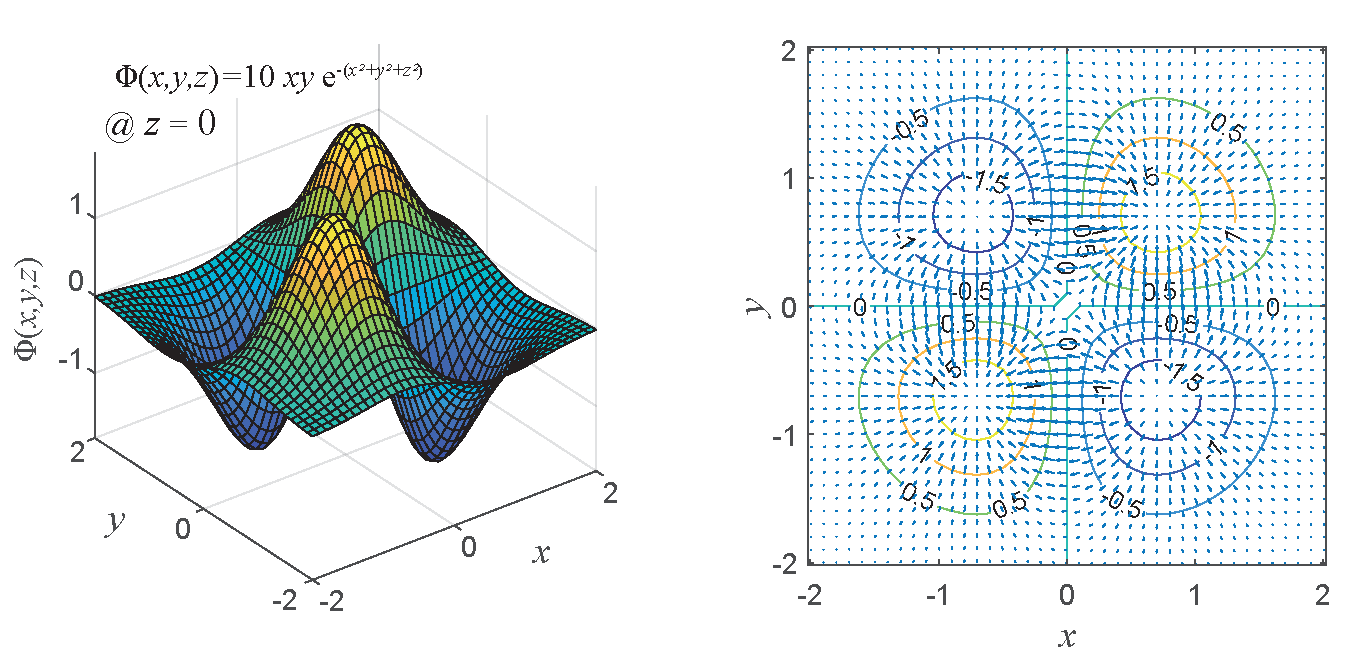
\includegraphics[width=\textwidth]{GradientExample.pdf}
    \caption[Funktion $\Phi = 10 x y \e^{-(x^2+y^2+z^2)}$ und Gradient der Funktion.]
    {Funktion $\Phi = 10 x y \e^{-(x^2+y^2+z^2)}$ und Gradient der Funktion.}
    \label{abb:kontmech_gradientexample1}
\end{figure}

\begin{figure}
    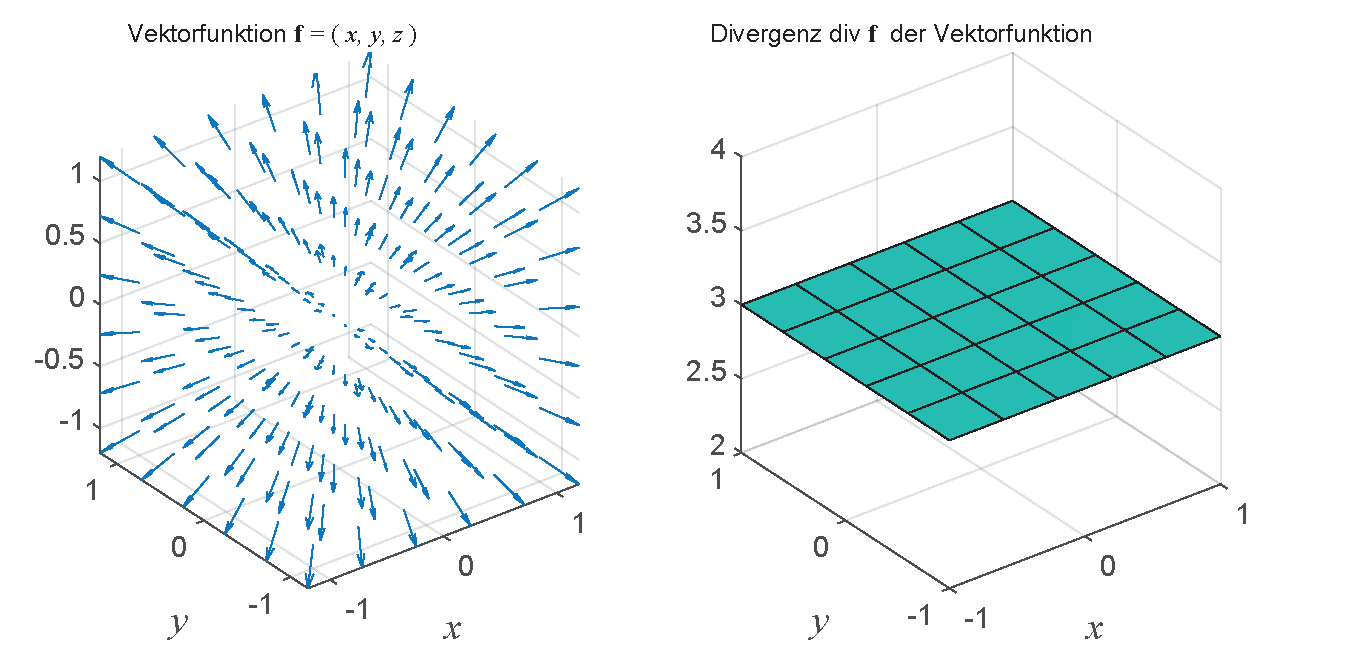
\includegraphics[width=\textwidth]{DivergenceExample.pdf}
    \caption[Vektorfunktion $\vec{f} = ( x, y, z ) $ und Divergenz der Funktion.]
    {Funktion $\vec{f}  = ( x, y, z ) $ und Divergenz der Funktion.}
    \label{abb:kontmech_divexample}
\end{figure}

\newpage
\begin{figure}
    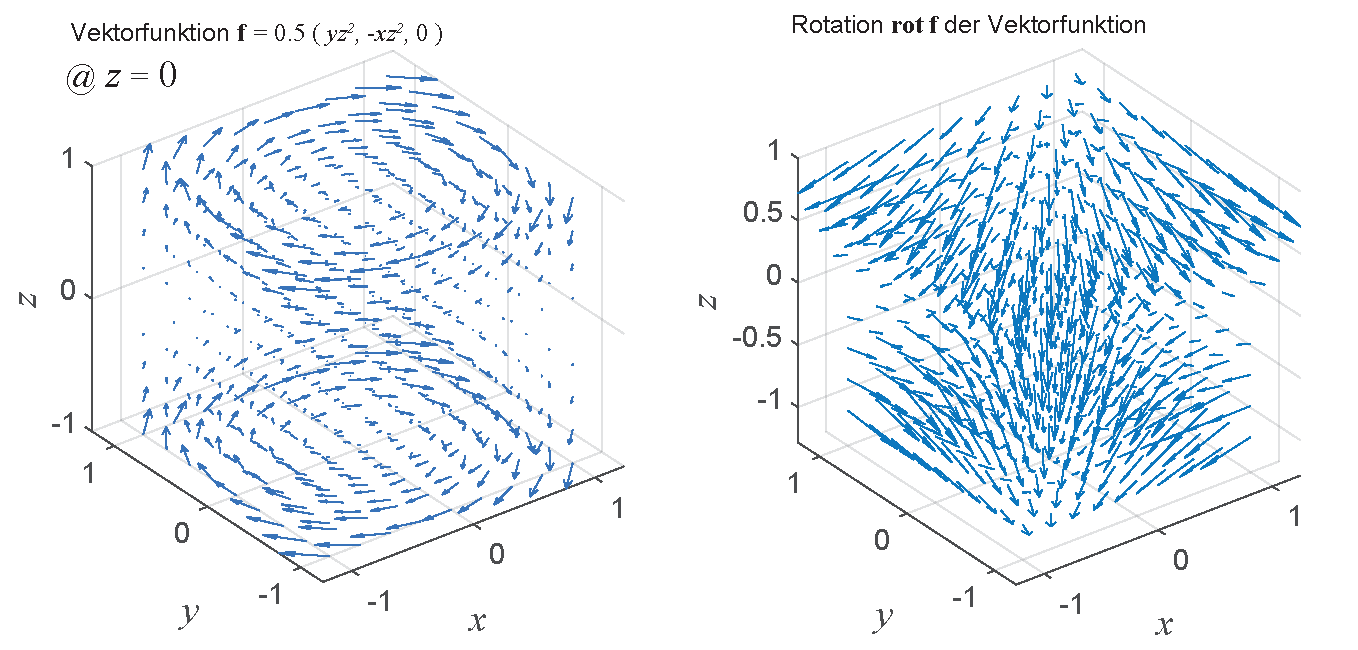
\includegraphics[width=\textwidth]{CurlExample.pdf}
    \caption[Vektorfunktion $\vec{f} = 0.5\,(yz^2, -xz^2, 0)$ und Rotation der Funktion.]
    {Funktion $\vec{f} = 0.5\,(yz^2, -xz^2, 0)$ und Rotation der Funktion.}
    \label{abb:kontmech_curlexample}
\end{figure}



\end{sol} 
\textcolor{blue} {$\rightarrow$ zur} \probref{kontmech_diffoperators}.\\
\noindent\rule[1ex]{\textwidth}{0.5pt}  \newpage  \clearpage

%-----------------------------------------------------------------------------------------------------------

\begin{sol}{prob:kontmech_ueb_vectoranalysis}\label{lsg:kontmech_ueb_vectoranalysis} %�bung2
\textbf{�bungen zur Vektorrechnung und Vektoranalysis}
\begin{enumerate}
    \item [a)] Wir geben exemplarisch die L�sung f�r die Gra�mann\footnote{Hermann G�nther Gra�mann (1809--1877) war ein deutscher Mathematiker und Physiker und einer der wesentlichen Wegbereiter der modernen Vektor- und Tensorrechnung.}-Identit�t \index{Gra�mann-Identit�t}\indexp{Gra�mann,Herrmann} $\vec{a} \times \lk \vec{b} \times \vec{c}\rk $ an, mit $\vec{a} = \lk a_1,a_2,a_3\rk^\intercal,\,\vec{b} = \lk b_1,b_2,b_3\rk^\intercal,\,\vec{c} = \lk c_1,c_2,c_3\rk^\intercal$:
    \begin{enumerate}
        \item [$\alpha$)] Rechnung in \textbf{kartesischen Koordinate}n:
        \begin{align}
            \vec{m} &= \vec{b} \times \vec{c} = 
						\begin{pmatrix}
                m_1 \\
                m_2\\
                m_3
            \end{pmatrix} =
            \begin{vmatrix}
                \vec{e_1} & b_1 & c_1\\
                \vec{e_2} & b_2 & c_2\\
                \vec{e_3} & b_3 & c_3\\
            \end{vmatrix}=
            \begin{pmatrix}
                b_2\,c_3 -b_3\,c_2\\
                b_3\,c_1-b_1\,c_3\\
                b_1\,c_2 -b_2\,c_1
            \end{pmatrix}\nonumber\\ 
            \vec{q} &= \vec{a}\times\vec{m} = 
            \begin{vmatrix}
                 \vec{e_1} & a_1 & m_1\\
                \vec{e_2} & a_2 & m_2\\
                \vec{e_3} & a_3 & m_3\\
            \end{vmatrix} =
            \begin{pmatrix}
                a_2\,m_3-a_3\,m_2\\
                a_3\,m_1-a_1\,m_3\\
                a_1\,m_2-a_2\,m_1
            \end{pmatrix}\nonumber \\
            &= 
            \begin{pmatrix}
                a_2\,b_1\,c_2 - a_2\,b_2\,c_1 - a_3\,b_3\,c_1 + a_3\,b_1\,c_3 \\
                a_3\,b_2\,c_3 - a_3\,b_3\,c_2 - a_1\,b_1\,c_2 + a_1\,b_2\,c_1 \\
                a_1\,b_3\,c_1 - a_1\,b_1\,c_3 - a_2\,b_2\,c_3 + a_2\,b_3\,c_2
            \end{pmatrix}
            = 
            \begin{pmatrix}
                b_1\,\lk a_2\,c_2 +a_3\,c_3\rk - c_1\,\lk a_2\,b_2 + a_3\,b_3\rk \\
                b_2\,\lk a_1\,c_1 +a_3\,c_3\rk - c_2\,\lk a_1\,b_1+a_3\,b_3\rk\\
                b_3\,\lk a_1\,c_1 +a_2\,c_2\rk - c_3\,\lk a_1\,b_1+a_2\,b_2\rk
            \end{pmatrix}\nonumber\\
            &= 
            \begin{pmatrix}
                b_1\,\lk a_i\,c_i\rk - \cancel{b_1\,a_1\,c_1} - c_1\,\lk a_i\,b_i\rk+ \cancel{c_1\,a_1\,b_1}\\
                b_2\,\lk a_i\,c_i\rk - \cancel{b_2\,a_2\,c_2} - c_2\,\lk a_i\,b_i\rk+ \cancel{c_2\,a_2\,b_2}\\
                b_3\,\lk a_i\,c_i\rk - \cancel{b_3\,a_3\,c_3} - c_3\,\lk a_i\,b_i\rk+ \cancel{c_3\,a_3\,b_3}
            \end{pmatrix}
            = \vec{b}\, \lk \vec{a} \,\vec{c} \rk - \vec{c}\, \lk \vec{a}\, \vec{b}\rk  \,.  \label{eq:kontmech_Ueb2_01} 
        \end{align}
        \item [$\beta$)] Rechnung mit \textbf{Levi-Civita-Symbol} und Einsteinscher Summenkonvention
        \begin{align}
            \vec{a}\times\vec{b} = \sum_{i=1}^3\sum_{j=1}^3\sum_{k=1}^3\,\epsilon_{ijk}\,a_i\,b_j\,\vec{e}_k=\epsilon_{ijk}\,a_i\,b_j\,\vec{e}_k \label{eq:kontmech_Ueb2_02}  \,. 
        \end{align}
        Damit:
        \begin{align}
            \vec{a}\times\underbrace{\lk \vec{b}\times\vec{c}\rk}_{\vec{m}} &=\epsilon_{ijk}\,a_i\,m_j\,\vec{e}_k ~~\rightarrow~~
            m_j = \epsilon_{\alpha\beta j}\,b_\alpha\,c_\beta ~~\rightarrow~~
           \lek \vec{a}\times\lk \vec{b}\times \vec{c}\rk \rek_k= \epsilon_{ijk}\,\epsilon_{\alpha\beta j}\,a_i\,b_\alpha\,c_\beta  \,. \label{eq:kontmech_Ueb2_03} 
        \end{align}
        Mit $\epsilon_{ijk} = -\epsilon_{ikj}$ und der Identit�t $ \epsilon_{\alpha\beta j}\,\epsilon_{ikj} = \delta_{\alpha i}\,\delta_{\beta k} - \delta_{\alpha k}\,\delta_{\beta i}$ erhalten wir:
        \begin{align}
            \epsilon_{\alpha\beta j}\,\epsilon_{ijk}\,b_\alpha\,a_i\,c_\beta &= -\epsilon_{\alpha\beta j}\,\epsilon_{ikj}\,b_\alpha\,a_i\,c_\beta 
            = \lk -\delta_{\alpha i}\,\delta_{\beta k} + \delta_{\alpha k}\,\delta_{\beta i}\rk\,b_\alpha\,a_i\,c_\beta \nonumber\\
            &= \delta_{\alpha k}\,b_\alpha\,\delta_{\beta i}\,a_i\,c_\beta - \delta_{\beta k}\,c_\beta\,\delta_{\alpha i}\,a_i\,b_\alpha 
             = \delta_{\alpha k}\,b_k\,a_i\,c_i - \delta_{\beta k}\,c_\beta\,a_i\,b_i \nonumber\\
            &= b_k\,\lk a_i\,c_i\rk -c_k\,\lk a_i\,b_i\rk ~~ \Leftrightarrow ~~\vec{a} \times \lk \vec{b} \times \vec{c}\rk = \vec{b}\,\lk \vec{a}\,\vec{c}\rk -\vec{c}\,\lk\vec{a}\,\vec{b}\rk\,. \label{eq:kontmech_Ueb2_05} 
        \end{align}
    \end{enumerate}
    \item [b)] Wir zeigen die Rechnung exemplarisch f�r \textbf{Zylinderkoordinaten} und bilden die Jacobi-Matrix f�r $q_1 =\rho\,\cos\phi,\,q_2= \rho\,\sin\phi,\,q_3=z$:
    \begin{align}
    \begin{split}
        \mathbb{J} = 
        \begin{pmatrix}
            \frac{\d x}{\d \rho} & \frac{\d x}{\d \phi} & \frac{\d x}{\d z} \\
            \frac{\d y}{\d \rho} & \frac{\d y}{\d \phi} & \frac{\d y}{\d z}\\
            \frac{\d z}{\d \rho} & \frac{\d z}{\d \phi} & \frac{\d z}{\d z}
        \end{pmatrix}
        &=
        \begin{pmatrix}
            \cos\phi & -\rho\,\sin\phi & 0 \\
            \sin\phi & \rho\cos\varphi & 0\\
            0&0&1
        \end{pmatrix}~~~~\text{sowie} ~~~\det \mathbb{J} = \rho
    \end{split} \,. \label{eq:kontmech_Ueb2_07}
    \end{align}
    Wir k�nnen nun schreiben
    \begin{align}
        \begin{pmatrix}
            \D x\\
            \D y\\
            \D z
        \end{pmatrix}
        = 
        \mathbb{J}\,
        \begin{pmatrix}
            \D \rho\\
            \D \phi\\
            \D z
        \end{pmatrix} ~~~\text{und f�r}~\det\mathbb{J}\neq 0: ~~~
        \begin{pmatrix}
            \D \rho\\
            \D \phi
            \D z
        \end{pmatrix}
        =
        \mathbb{J}^{-1}\,
        \begin{pmatrix}
            \D x\\
            \D y\\
            \D z
        \end{pmatrix}  \,. \label{eq:kontmech_Ueb2_09}
    \end{align}
    Die Spalten der Jacobi-Matrix sind gerade die Differentiale $\d\vec{r}/\d q_j$, was uns erlaubt, den neuen Einheitsvektor $\vec{e}_{q_j}$, wie man leicht nachrechnen kann, wie folgt zu schreiben 
    \begin{align}
        \vec{e}_{q_j} = \frac{1}{h_j}\,\frac{\d \vec{r}\lk q_k\rk}{\d q_j} ~~~ \text{mit} ~~~ j=1,2,3 ~~~~~~ \text{mit}~~~h_j =
        \begin{vmatrix}
            \frac{\d \vec{r}}{\d q_j}
        \end{vmatrix}  \,. \label{eq:kontmech_Ueb2_11}
    \end{align}
   Die Gr��en $h_j$ hei�en Skalenfaktoren. Unter Benutzung von \eqref{eq:kontmech_Ueb2_07} finden wir \zb f�r Zylinderkoordinaten mit $\vec{r} = \rho\,\cos\phi\,\vec{e}_x+\rho\,\sin\phi\,\vec{e}_y + z\,\vec{e}_z$ die folgenden Skalenfaktoren:
    \begin{align*}
        h_1 &= |\cos\rho\,\vec{e}_x + \sin\phi\,\vec{e}_y| = 1\,,\\
        h_2 &= |-\rho\,\sin\phi\,\vec{e}_x +\rho\,\cos\phi\,\vec{e}_y| = \rho\,,\\
        h_3 &= |\vec{e}_z| =1\,,
    \end{align*}
    woraus sich leicht die neuen orthogonalen Einheitsvektoren nach \eqref{eq:kontmech_Ueb2_11} berechnen lassen:
    \begin{align}
    \begin{split}
        \vec{e}_\rho &= \lk\cos\varphi,\sin\varphi,0\rk^\intercal\,,\\
        \vec{e}_\phi &= \frac{1}{\rho}\lk -\sin\varphi,\cos\varphi,0\rk^\intercal\,,\\
        \vec{e}_z &= \lk 0,0,1\rk^\intercal\,.
    \end{split}\label{eq:kontmech_Ueb2_12}
    \end{align}
    Wir erkennen hier die Spalten der Jacobi-Matrix wieder. Das Volumenelement, welches \zb f�r die Integration in den neuen Koordinaten ben�tigt wird, berechnet man am einfachsten �ber das Spatprodukt\index{Spatprodukt}. Man erh�lt:
    \begin{align}
    \begin{split}
        \D V &= h_1\,\D q_1\,\vec{e}_{q_1}\,\lk h_2\,\D q_2\,\vec{e}_{q_2} \times h_3\,\D q_3\,\vec{e}_{q_3}\rk = \sum_{j=1}^3\,h_j\,\D q_j = h_a\,h_2\,h_3\,\D q_1\,\D q_2\,\D q_3
    \end{split}  \,. \label{eq:kontmech_Ueb2_13}
    \end{align}
    und speziell f�r Zylinderkoordinaten:
    \begin{align}
        \D V = \rho\,\D\rho\,\D \phi\,\D z \label{eq:kontmech_Ueb2_14}\,.
    \end{align}
    Mit der Beziehung \eqref{eq:kontmech_Ueb2_11} kann man leicht die Beziehung f�r einen Gradienten \bzw den Nabla-Operator $\vec{\nabla}$ aus \eqref{eq:kontmech_nabladef} berechnen:
    \begin{align*}
        \D \Phi &= \frac{\D\Phi}{\d q_j}\,\D q_j = \nabla\Phi\,\D \vec{r}\,,~~~~ \D \vec{r} = \frac{\d \vec{r}}{\d q_j}\,\D q_j\,\vec{e}_j= h_j\,\D q_j\,\vec{e}_{q_j} \\
        \rightarrow ~~ \D \Phi &= \frac{\d \Phi}{\D q_j}\,\D q_j = \nabla\Phi\,h_j\,\D q_j\,\vec{e}_{q_j}  \,. 
    \end{align*}
    Aus dem Vergleich beider Seiten finden wir:
    \begin{align}
        \nabla = \frac{1}{h_j}\,\frac{\d}{\d q_j}\,\vec{e}_{q_j} =  \lk \frac{1}{h_1}\,\frac{\d}{\d q_1},\,\frac{1}{h_2}\,\frac{\d}{\d q_2},\,\frac{1}{h_3}\,\frac{\d}{\d q_3}\rk  \,. \label{eq:kontmech_Ueb2_15}
    \end{align}
    Speziell f�r Zylinderkoordinaten:
    \begin{align}
        \nabla = \lk \frac{\d}{\d \rho},\frac{1}{\rho}\,\frac{\d}{\d\phi},\frac{\d}{\d z }\rk \,. \label{eq:kontmech_Ueb2_17}
    \end{align}
    Aus der leicht zu berechnenden Jacobi-Matrix f�r sph�rische Koordinaten
    \begin{align}
        J = 
        \begin{pmatrix}
            \frac{\d x}{\d r} & \frac{\d x}{\d \theta} &  \frac{\d x}{\d \phi}\\
            \frac{\d y}{\d r} & \frac{\d y}{\d \theta} &  \frac{\d y}{\d \phi}\\
            \frac{\d z}{\d r} & \frac{\d z}{\d \theta} &  \frac{\d z}{\d \phi}
        \end{pmatrix}
        =
        \begin{pmatrix}
            \sin\theta\,\cos\phi & r\,\cos\theta\,\cos\phi & -r\,\sin\theta\,\sin\phi\\
            \sin\theta\,\sin\phi & r\,\cos\theta\,\sin\phi & -r\,\sin\theta\,\cos\phi\\
            \cos\theta & -r\,\sin\theta & 0
        \end{pmatrix}  \,. \label{eq:kontmech_Ueb2_18}
    \end{align}
    \begin{align}
        J^{-1} = 
        \begin{pmatrix}
            \frac{\d r}{\d x} & \frac{\d r}{\d  y} &  \frac{\d r}{\d z}\\
            \frac{\d \theta}{\d x} & \frac{\d \theta}{\d y} &  \frac{\d \theta}{\d z}\\
            \frac{\d \phi}{\d x} & \frac{\d \phi}{\d y} &  \frac{\d \phi}{\d z}
        \end{pmatrix}
        =
        \begin{pmatrix}
            \sin\theta\,\cos\phi & \sin\theta\,\sin\phi & \cos\theta\\
            \frac{1}{r}\,\cos\theta\,\cos\phi & \frac{1}{r}\,\cos\theta\,\sin\phi & -\frac{1}{r}\,\sin\theta \\
            -\frac{1}{r}\,\frac{\sin\phi}{\sin\theta} & \frac{1}{r}\,\frac{\cos\phi}{\sin\theta} & 0
        \end{pmatrix}  \label{eq:kontmech_Ueb2_19}
    \end{align}
    mit 
    \begin{align}
        \det\lk J\rk= r^2\,\sin\theta \label{eq:kontmech_Ueb2_20}
    \end{align}
    finden wir mit 
    \begin{align*}
        h_1 &= 1\,,~~~h_2 = \frac{1}{r\,\sin\theta}\,,~~~h_3 = \frac{1}{r}
    \end{align*}
    schlie�lich
    \begin{align}
        \nabla = \lk \frac{\d}{\d r},\frac{1}{r\,\sin\theta}\,\frac{\d}{\d \phi},\frac{1}{r}\,\frac{\d}{\d\theta}\rk\,. \label{eq:kontmech_Ueb2_21}
    \end{align}
		
		
    Die weiteren \textbf{Differentialoperatoren} $\divv$, $\rotv$, $\Delta$ findet man leicht mit Hilfe des Nabla-Kalk�ls, \zb erhalten wir f�r die Divergenz:
    \begin{align*}
        \divv \vec{f} = \nabla\,\vec{f} = \nabla\,\lk f_j\,\vec{e}_{q_j}\rk = \nabla \,\lk f_j\,\epsilon_{\alpha\beta j}\,\vec{e}_{q_\alpha} \times \vec{e}_{q_\beta}\rk\,.
    \end{align*}
    Dabei haben wir ber�cksichtigt, dass die $\vec{e}_{q_i}$ ein Rechtssystem bilden. Wir wollen diese Beziehung zun�chst f�r $j=1$ auswerten und erhalten mit \eqref{eq:kontmech_Ueb2_15}
    \begin{align*}
        \nabla\,\lk f_1\,\vec{e}_{q_2} \times \vec{e}_{q_3} \rk = \nabla\,\lk f_1\,h_2\,\nabla\,q_2\times h_3\,\nabla\,q_3\rk  \,. 
    \end{align*}
    Wir benutzen:
    \begin{align}
        \nabla q_1 &= \lk\frac{1}{h_1}\,\frac{\d q_1}{\d q_1},\underbrace{\frac{1}{h_2}\,\frac{\d q_1}{\d q_2}}_{=0},\underbrace{\frac{1}{h_3}\,\frac{\d q_1}{\d q_3}}_{=0}\rk~~\rightarrow ~~~~ h_1\,\nabla\,q_1 = \vec{e}_{q_1}  \,. 
    \end{align}
    \begin{align*}
        \nabla\,\lk f_1\,h_2\,\nabla\,q_2\times h_3\,\nabla\,q_3\rk &= \nabla\,\lk f_1\,h_2\,h_3 \,\lk \nabla\,q_2\times\nabla\,q_3\rk \rk \\
        &= \nabla\,\lk f_1\,h_2\,h_3\rk\,\cdot \lk \nabla q_2\times\nabla\,q_3\rk + f_1\,f_2\,h_3\,\underbrace{\nabla\,\lk \nabla\,q_2\times\nabla\,q_2\rk}_{=0}\\
        &= \nabla\,\lk f_1\,h_2\,h_3\rk\cdot\lk\frac{\vec{e}_2}{h_2}\times\frac{\vec{e}_3}{h_3}\rk = \nabla\,\lk f_1\,h_2\,h_3\rk\cdot\frac{\vec{e}_1}{h_2\,h_3}r\\
        &= \lek \frac{1}{h_1}\,\frac{\d \lk f_1 h_2 h_3 \rk}{\d q_1}\,\vec{e}_1+\ldots\,\vec{e}_2+\ldots\,\vec{e}_3\rek\cdot\frac{\vec{e}_1}{h_2\,h_3} = \frac{1}{h_1\,h_2\,h_3}\,\frac{\d}{\d q_1}\,\lk f_1\,h_2\,h_3\rk  \,. 
    \end{align*}
    Analog f�r $j=2,3$ in \eqref{eq:kontmech_Ueb2_15} erh�lt man:
    \begin{align}
        \divv \vec{f} &= \nabla\,\vec{f} = \frac{1}{h_1\,h_2\,h_3}\,\lek \frac{\d}{\d q_1}\,\lk h_2\,h_3\,f_1\rk + \frac{\d}{\d q_2}\,\lk h_3\,h_1\,f_2\rk + \frac{\d}{\d q_3}\,\lk h_1\,h_2\,f_3\rk\rek \,.\label{eq:kontmech_Ueb2_23}  
    \end{align}
    
		Alternativ kann die \textbf{Divergenz} auch mit Hilfe des \textbf{Integralsatzes von Gau�} berechnet werden:
    \begin{align*}
        \iiint_{\text{Vo}}\divv\,\vec{f}\,\D V = \iint_{\d \text{Vo}}\,\lk \vec{f}\,\vec{n}\rk\,\D A \,.
    \end{align*}
    Das Volumen, �ber das integriert wird, soll ein sehr kleines Parallelepiped sein, das von den kleinen krummlinigen Rechtecken in den drei Koordinatenebenen $q_1,q_1+\D q_1;q_2,q_2 +\D q_2;q_3,q_3 + \D q_3$ begrenzt wird; die Seitenl�ngen dieser Rechtecke sind durch $\D s_1,\D s_2,\D s_3$ gegeben. \\
    Das Volumen ist so klein, dass sich das Vektordifferential darin kaum �ndert und daher vor das Integral gezogen werden kann; das verbleibende Integral ist dann das kleine Volumenelement $\D V$. Damit ergibt sich folgender Ausdruck f�r die Divergenz:
    \begin{align}
        \divv\,\vec{f} = \frac{1}{\D V}\,\iint_{\d \text{Vo}}\,\lk \vec{f}\,\vec{n}\rk\,\D A := I_1+I_2+I_3\,.\label{eq:kontmech_Ueb2_24}
    \end{align}
    Das Oberfl�chenintegral $I$ wird n�herungsweise berechnet, indem der Wert von $\lk \vec{f}\,\vec{n}\rk$ mit der Gr��e der Fl�che multipliziert wird. Dann ergibt sich f�r die zwei Fl�chen $q_3$ und $q_3 + \D q_3$:
    \begin{align*}
        \text{Fl�che}\,q_3:\,&-\lk f_3\,h_1\,h_2\rk_{q_3}\,\D q_1\,\D q_2\,,\\
         \text{Fl�che}\,q_3 + \D q_3:\,&+\lk f_3\,h_1\,h_2\rk_{q_3+\D q_3}\,\D q_1\,\D q_2 \\
         &~~=\lk f_3\,h_1\,h_2\rk_{q_3}\,\D q_1\,\D q_2 + \frac{\d}{\d q_3}\,\lk f_3\,h_1\,h_2\rk_{q_3}\,\D q_3\,\D q_2\,\D q_2\,.
    \end{align*}
    Die Indices $q_3$ \bzw $q_3+\D q_3$ geben an, dass die Funktion in der Klammer an $q_3$ \bzw $q_3 + \D q_3$ zu berechnen ist. Die Summer obiger Terme gibt dann:
    \begin{align*}
        I_3= \frac{\d}{\d q_3}\,\lk f_3\,h_1\,h_2\rk\,\D q_1\,\D q_2\,\D q_3\,.
    \end{align*}
    Analog berechnet man die Integrale $I_1$ und $I_2$:
    \begin{align*}
        I_1&= \frac{\d}{\d q_1}\,\lk f_1\,h_2\,h_3\rk\,\D q_1\,\D q_2\,\D q_3\,,~~~I_2= \frac{\d}{\d q_2}\,\lk f_2\,h_2\,h_3\rk\,\D q_1\,\D q_2\,\D q_3\,.
    \end{align*}
    Die Summe $I_1+I_2+I_3$ wird durch das infinitesimale Volumen $\D V = h_1\,h_2\,h_3\,\D q_1\,\D q_2\,\D q_3$ dividiert. Dabei k�rzen sich die Differentiale und man erh�lt wieder den Ausdruck f�r die Divergenz, der nat�rlich mit \eqref{eq:kontmech_Ueb2_23} �bereinstimmt:
    \begin{align}
        \divv\,\vec{f} = \frac{1}{h_1\,h_2\,h_3}\,\lek \frac{\d}{\d q_1}\,\lk f_1\,h_2\,h_3\rk+\frac{\d}{\d q_2}\,\lk f_2\,h_1\,h_3\rk + \frac{\d}{\d q_3}\,\lk f_3\,h_2\,h_3\rk\rek \,. \label{eq:kontmech_Ueb2_25}
    \end{align}
		
    Eine Herleitung der \textbf{Rotation} findet man entsprechend �ber den \textbf{Integralsatz von Stokes}.
    \begin{align}
        \rotv\,\vec{f} = \iint_{\text{Ar}}\rotv\,\vec{f}\,\D \vec{A} = \oint\limits_{\d \text{Ar}}\vec{f}\,\D \vec{r}\,.\label{eq:kontmech_Ueb2_26}
    \end{align}
    Wir finden:
    \begin{align}
        \rotv\,\vec{f} = \nabla\times\vec{f} = \frac{1}{h_1\,h_2\,h_3}\,
        \begin{vmatrix}
            h_1\,\vec{e}_{q_1} & h_2\,\vec{e}_{q_2} & h_3\,\vec{e}_{q_3} \\
            \frac{\d}{\d q_1} & \frac{\d}{\d q_2} & \frac{\d}{\d q_3} \\
            h_1\,f_1 & h_2\,f_2 & h_3\,f_3
        \end{vmatrix} \,. \label{eq:kontmech_Ueb2_27}
    \end{align}
    
		F�r den \textbf{Laplace-Operator} $\Delta$ finden wir:
    \begin{align}
        \Delta\Phi = \nabla^2\Phi =\,&\frac{1}{h_1\,h_2\,h_3}\,\lek \frac{\d}{\d q_1}\,\lk \frac{h_2\,h_3}{h_1}\,\frac{\d \Phi}{\d q_1}\rk + \frac{\d}{\d q_2}\,\lk \frac{h_1\,h_3}{h_2}\,\frac{\d \Phi}{\d q_2}\rk + \frac{\d}{\d q_3}\,\lk \frac{h_2\,h_3}{h_3}\,\frac{\d \Phi}{\d q_3}\rk\rek \,.
    \end{align}\\
    
	 Zusammenfassend finden wir f�r \textbf{sph�rische Koordinaten}
    \begin{subequations}
    \begin{align}
        \nabla\Phi &= \frac{\d\Phi}{\d r}\,\hat{\vec{e}}_r + \frac{1}{r}\,\frac{\d\Phi}{\d\theta}\,\hat{\vec{e}}_\theta + \frac{1}{r\,\sin\theta}\,\frac{\d\Phi}{\d\phi}\,\hat{\vec{e}}_\phi  \,,\\
        \nabla\,\vec{f} &= \frac{1}{r^2}\,\frac{\d}{\d r}\,\lk r^2\,f_r\rk + \frac{1}{r\,\sin\theta\,\frac{\d}{\d \theta}}\,\lk \sin\theta\,f_\theta\rk + \frac{1}{r\,\sin\theta}\,\frac{\d f_\phi}{\d \phi}  \,,\\
        \nabla\times\vec{f} &= \frac{1}{r^2\,\sin\theta}\,
        \begin{vmatrix}
            \hat{\vec{e}}_r &  r\,\hat{\vec{e}}_\theta & r\,\sin\theta\,\hat{\vec{e}}_\phi\\
            \frac{\d}{\d r} & \frac{\d}{\d \theta} & \frac{\d}{\d \phi}  \,,\\
            f_r & r\,f_\theta & r\,\sin\theta\,f_\phi
        \end{vmatrix} \\
        \Delta\Phi &= \frac{1}{r^2}\,\frac{\d}{\d r}\,\lk r^2\,\frac{\d \Phi}{\d r}\rk + \frac{1}{r^2\,\sin\theta}\,\frac{\d}{\d\theta}\,\lk\sin\theta\,\frac{\d \Phi}{\d \theta}\rk + \frac{1}{r^2\,\sin^2\theta}\,\frac{\d^2\Phi}{\d \phi^2}  \,. 
    \end{align}\label{eq:kontmech_Ueb2_28}
    \end{subequations} 
    und analog f�r die \textbf{Zylinderkoordinaten}:
    \begin{subequations}
    \begin{align}
        \nabla\Phi &= \frac{\d\Phi}{\d \rho}\,\hat{\vec{e}}_\rho + \frac{1}{\rho}\,\frac{\d\Phi}{\d\phi}\,\hat{\vec{e}}_\phi + \frac{\d\Phi}{\d z}\,\hat{\vec{e}}_x \,,\\
        \nabla\,\vec{f} &= \frac{1}{\rho}\,\frac{\d}{\d \rho}\,\lk\rho\,f_\rho\rk + \frac{1}{\rho}\,\frac{\d f_\phi}{\d \phi} + \frac{\d f_z}{\d z} \,,\\
        \nabla\times\vec{f}&= \frac{1}{\rho}\,
        \begin{vmatrix}
            \hat{\vec{e}}_\rho & \rho\,\hat{\vec{e}}_\phi & \hat{\vec{e}}_z \\
            \frac{\d}{\d \rho} & \frac{\d}{\d \phi} & \frac{\d}{\d z} \\
            f_\rho & \rho\,f_\phi & f_z
        \end{vmatrix}  \,,\\
        \nabla^2\,\Phi &= \frac{1}{\rho}\,\frac{\d}{\d\rho}\,\lk\rho\,\frac{\d\Phi}{\d \rho} + \frac{1}{\rho^2}\,\frac{\d^2\Phi}{\d \phi^2} + \frac{\d^2\Phi}{\d z^2}\rk  \,.
    \end{align}\label{eq:kontmech_Ueb2_29}
    \end{subequations}
    \item[c)] Wir berechnen nun noch die \textbf{Geschwindigkeit und Beschleunigung in Zylinderkoordinaten}:
    \begin{align}
    \begin{split}
        \vec{r} &= \rho\,\vec{e}_\rho + z\,\vec{e}_z  \,,\\
        \dot{\vec{r}} &= \dot{\rho}\,\vec{e}_\rho+\dot{z} \vec{e}_z + \rho\,\dot{\vec{e}}_\rho + z\,\dot{\vec{e}}_z = \dot{\rho}\,\vec{e}_\rho + \dot{z}\,\vec{e}_z + \rho\,
        \underbrace{
        \begin{pmatrix}
            -\sin\varphi\\
            \cos\varphi\\
            0
        \end{pmatrix}
        }_{=\vec{e}_\phi}\,\dot{\phi} +0 = \dot{\rho}\,\vec{e}_\rho  + \rho\,\dot{\phi} \,\vec{e}_\phi + \dot{z}\,\vec{e}_z  \,.
    \end{split}\label{eq:kontmech_Ueb2_30}
    \end{align}
    \begin{align}
    \begin{split}
        \ddot{\vec{r}} &= \ddot{\rho}\,\vec{e}_\rho + \dot{\rho}\,\dot{\phi}\,\vec{e}_\rho + \rho\,\ddot{\phi}\,\vec{e}_\phi + \ddot{z}\,\vec{e}_z +\dot{\rho}\,\dot{\vec{e}}_\rho + \rho\,\dot{\phi}\,\dot{\vec{e}}_\phi~~~\text{mit}~~~
        \dot{\vec{e}}_\rho = 
        \underbrace{
        \begin{pmatrix}
            -\sin\varphi\\
            \cos\varphi\\
            0
        \end{pmatrix}
        }_{=\vec{e}_\phi}\,\dot{\phi} ~~~\text{und}~~~\dot{\vec{e}}_\phi = 
        \underbrace{
        \begin{pmatrix}
            -\rho\,\sin\phi\\
            \rho\,\cos\phi\\
            0
        \end{pmatrix}
        }_{=-\vec{e}_\rho\,\dot{\phi}}\,\dot{\phi}\\
        &= \lk \ddot{\rho} -\rho\,\dot{\phi}^2\rk \, \vec{e}_\rho + \lk 2\dot{\rho}\,\dot{\phi} + \rho\,\ddot{\phi}\rk\,\vec{e}_\phi + \ddot{z}\,\vec{e}_z  \,.
    \end{split}\label{eq:kontmech_Ueb2_31}
    \end{align}
\end{enumerate}
\end{sol} 
\textcolor{blue} {$\rightarrow$ zur} \probref{kontmech_ueb_vectoranalysis}.\\
\noindent\rule[1ex]{\textwidth}{0.5pt}  \newpage  \clearpage


%-----------------------------------------------------------------------------------------------------------

\begin{sol}{prob:kontmech_integralsaetze}\label{lsg:kontmech_integralsaetze} %�bung3
\textbf{Integrals�tze der Vektoranalysis}
\begin{enumerate}
    \item [1)]
    \begin{align*}
        \vec{f}_1\lk \vec{r}\rk &= 0.5\,
        \begin{pmatrix}
            y\,z^2\\
            -x\,z^2\\
            0
        \end{pmatrix} 
				~~\rightarrow~~ \divv \vec{f}_1\lk\vec{r}\rk = 0 \quad \rotv \vec{f}_1\lk\vec{r}\rk = 
        \begin{pmatrix}
            x\,z\\
            y\,z\\
            -z^2
        \end{pmatrix} \\
        \vec{f}_2\lk \vec{r}\rk &= 
        \begin{pmatrix}
            0\\
            2x\,z + 3y^2\\
            4y\,z^2
        \end{pmatrix}
       ~~\rightarrow~~\divv \,\vec{f}_2\lk\vec{r}\rk = 0+6y+8y\,z = y\,\lk 3+4z\rk \quad  \rotv \vec{f}_2\lk\vec{r}\rk = 
        \begin{pmatrix}
            -2x+4z^2\\
            0\\
            2z
        \end{pmatrix}
    \end{align*}
    \begin{enumerate}
        \item [a)] \underline{Integralsatz von Gau� f�r $\vec{f}_1$}
        \begin{align*}
            \int\limits_{\text{Vo}} \divv \vec{f}_1\,\D V = 0 = \iint\limits_{\d \text{Vo}}\vec{f}_1\,\D \vec{A} = I
        \end{align*}
        Wir betrachten den Einheitskubus $V_o = \lek 0,1;0,1;0,1\rek$ mit den Au�enfl�chen:
        \begin{align*}
            A1:\,z=0,\,x=\lek 0,1\rek,\,y=\lek 0,1\rek ~~~~ \lk -\vec{e}_z-\text{Richtung}\rk \\
            A2:\,z=1,\,x=\lek 0,1\rek,\,y=\lek 0,1\rek ~~~~ \lk +\vec{e}_z-\text{Richtung}\rk\\
            A3:\,x=0,\,y=\lek 0,1\rek,\,z=\lek 0,1\rek ~~~~ \lk -\vec{e}_x-\text{Richtung}\rk\\
            A4:\,x=1,\,y=\lek 0,1\rek,\,z=\lek 0,1\rek ~~~~ \lk +\vec{e}_x-\text{Richtung}\rk \\
            A5:\,y=0,\,x=\lek 0,1\rek,\,z=\lek 0,1\rek ~~~~ \lk -\vec{e}_y-\text{Richtung}\rk\\
            A6:\,y=1,\,x=\lek 0,1\rek,\,z=\lek 0,1\rek ~~~~ \lk +\vec{e}_y-\text{Richtung}\rk
        \end{align*}
        \begin{align*}
            I_1 &= \int\limits_0^1\int\limits_0^1\,\vec{f}_1\,\lk z=0,x,y\rk\,\vec{e}_z\,\vec{e}_z\,\D x \D y = 0\quad\quad
            I_2 = \int\limits_0^1\int\limits_0^1\,\lk y\,z^2\,\vec{e}_x - x\,z^2\,\vec{e}_y\rk\,\vec{e}_z\,\D x \D y = 0\\
            I_3 &= \int\limits_0^1\int\limits_0^1\,y\,z^2\,\vec{e}_x\,\lk -\vec{e}_x\rk\,\D z\,D y = -\frac{1}{6}\quad\quad\quad
            I_4 = \int\limits_0^1\int\limits_0^1\,y\,z^2\,\vec{e}_x\,\lk \vec{e}_x\rk\,\D y\,D z = \frac{1}{6}\\
            I_5 &= \int\limits_0^1\int\limits_0^1\,-x\,z^2\,\vec{e}_y\,\lk - \vec{e}_y\rk\,\D x\,D z = \frac{1}{6}\quad\quad\quad
            I_6 = \int\limits_0^1\int\limits_0^1\,-x\,z^2\,\vec{e}_y\,\lk \vec{e}_y\rk \D x \D z = -\frac{1}{6}\\
            I &= \sum_{i=1}^6\,I_i = 0\\
        \end{align*}
        \item [b)] \underline{Integralsatz von Gau� f�r $\vec{f}_2$}
        \begin{align*}
            \int\limits_{\text{Vo}} \divv \vec{f}_2 \,\D V &= \int\limits_0^1\int\limits_0^1\int\limits_0^1 \lk 6y + 8y\,z\rk\,\D x \D y \D z = \int\limits_0^1\int\limits_0^1\lk 6y+8y\,z\rk\,\D y \D z = \int\limits_0^1\lk 3y^2+4y^2\,z\rk\, \D z = 5
        \end{align*}
        Wir betrachten wiederum den Einheitskubus mit den 6 Au�enfl�chen:
        \begin{align*}
             I_1 &= \int\limits_0^1\int\limits_0^1 -4y\,z^2 \D x \D y \,\Big|_{z=0} = 0\quad\quad\quad\quad
             I_2 = \int\limits_0^1\int\limits_0^1 4y\,z^2 \,\Big|\D x \D y =2\\
             I_3 &= \int\limits_0^1\int\limits_0^1 0\,\vec{e}_x\,\lk -\vec{e}_x\rk \,\D y\D z = 0\quad\quad\quad\quad
             I_4 = \int\limits_0^1\int\limits_0^1 0\,\vec{e}_x\,\lk +\vec{e}_x\rk \D y \D z = 0 \\
             I_5 &= \int\limits_0^1\int\limits_0^1 2x\,z\,\vec{e}_y\,\lk -\vec{e}_y\rk \D x \D z = -\frac{1}{2}\quad\quad
             I_6 = \int\limits_0^1\int\limits_0^1\lk 2x\,z+3\rk\,\vec{e}_y\,\lk +\vec{e}_y\rk \D x \D z = \frac{7}{2}\\
             I &= \sum_{i=1}^6 I_i = 2-\frac{1}{2}+3+\frac{1}{2} = 5
        \end{align*}
        Man sieht, dass manchmal die Volumenintegrale �ber die Divergenz oft einfacher zu berechnen sind als die Oberfl�chenintegrale, manchmal aber auch umgekehrt.
    \end{enumerate}
    \item[2)] F�r den Satz von Stokes betrachten wir exemplarisch das Einheitsquadrat bei $z=1$ parallel zur $x-y$-Ebene.
    \begin{enumerate}
        \item [a)] Funktion $\vec{f}_1$:
        \begin{align*}
        \int\limits_\text{Ar} \rotv \vec{f}_1\,\D \vec{A} = \int\limits_0^1\int\limits_0^1 -z^2\,\vec{e}_z\,\vec{e}_z \D x \D y \,\Big|_{z=1} =-1
        \end{align*}
        F�r das Linienintegral haben wir vier Abschnitte.
        \begin{align*}
            \int\limits_{\d \text{Ar}} \vec{f}_1 \D \vec{r} = I_1 + I_2+I_3+I_4
        \end{align*}
        \begin{align*}
            I_1: y=0,\,x=\lek 0,1\rek\quad\quad I_2: x=1,\,y=\lek 0,1\rek\quad \quad 
            I_3: y=1,\,x=\lek 0,1\rek\quad\quad I_4: x=0,\,y=\lek 0,1\rek\\
        \end{align*}
        \begin{align*}
            I_1 &= \int\limits_0^1 \frac{1}{2}\,y\,z^2\,\vec{e}_x\,\vec{e}_x\, \D x\,\Big|_{z=1,y=0} = 0\quad\quad\quad\quad\quad\quad
            I_2 = \frac{1}{2}\,\int\limits_0^1 -x\,z^2,\vec{e}_y\,\vec{e}_y\,\D y\,\Big|_{x,z=1} = \frac{1}{2}\,y\,\Big|_0^1 =-\frac{1}{2}\\
            I_3 &= \frac{1}{2}\,\int\limits_1^0 y\,z^2,\vec{e}_x\,\vec{e}_x\,\D x\,\Big|_{y,z=1} = \frac{1}{2}\,x\,\Big|_1^0 =-\frac{1}{2}\quad\quad
            I_4 = \frac{1}{2}\,\int\limits_0^1 -x\,z^2,\vec{e}_y\,\vec{e}_y\,\D y\,\Big|_{x=0,z=1} = 0\,y\,\Big|_1^0 =0\\
            I &= \sum_{i=1}^4 I_i = -1
        \end{align*}
        \item [b)] Funktion $\vec{f}_2$:
        \begin{align*}
            \int\limits_\text{Ar} \rotv \vec{f}_2 \,\D \vec{A} = \int\limits_0^1 \int\limits_0^1 2z \, \vec{e}_z \vec{e}_z \,\D x \D y =2
        \end{align*}
        \begin{align*}
            I_1 &= \int\limits_0^1 0\,\vec{e}_x\,\vec{e}_x\,\D x = 0\quad\quad\quad
            I_2 = \int\limits_0^1\lk 2x\,z+3y^2\rk\,\vec{e}_y\,\vec{e}_y \D y\,\Big|_{x,z=1} = 2y+y^3\,\Big|_0^1 = 3 \\
            I_3 &= \int\limits_1^0 0\,\vec{e}_x\,\vec{e}_x\,\D x = 0\quad\quad\quad
            I_4 = \int\limits_1^0 3y^2\,\vec{e}_y\,\vec{e}_y\,\D y\,\Big|_{x,z=1} = -\frac{3}{3}\,y^3\,\Big|_1^0= -1 \\
            I&= \sum_{i=0}^4\,I_i =2
        \end{align*}
    \end{enumerate}
    \item [3)] Die Divergenz von $\vec{f}\lk \vec{r}\rk$ ist gegeben durch:
    \begin{align*}
        \divv \begin{pmatrix}
            2x+3z\\
            -x\,z-\\
            y^2+2z
        \end{pmatrix} =
        \lk 2+\lk -1\rk +2\rk =3\,.
    \end{align*}
    Das Volumen der Kugel mit Radius 3 ist $\frac{4}{3}\,\pi\,3^3$, so dass der Gau�sche Integralsatz
    \begin{align*}
        \int\limits_{\d v_0}\vec{f}\,\D \vec{A} = \int\limits_{v_0} 3\,\D v = \cancel{3}\,\frac{4}{\cancel{3}}\,\pi\,3^3  = 108\,\pi
    \end{align*}
     ergibt. Hier ist offensichtlich, wie viel einfacher die Berechnung �ber das Volumenintegral ist. 
    \item [4)] F�r ein Vektorfeld $\vec{f}$ welches die Divergenz $\divv \vec{f} = 1$ hat, kann man das Volumen �ber
    \begin{align*}
        V=\int\limits_\text{Vo} \,\D V = \int\limits_\text{Vo} \divv \vec{f}\,\D V = \int\limits_{\d \text{Vo}}\,\vec{f}\,\D \,\vec{A}
    \end{align*}
    durch das Oberfl�chenintegral berechnen.
    \begin{enumerate}
        \item [i)] Wir nehmen als Funktion $\vec{f} = \frac{1}{2}\,\lk x,y,0\rk$ und k�nnen in dem wir Zylinderkoordinaten verwenden f�r das Volumen schreiben:
        \begin{align*}
            V = \int\limits_{\d \text{Vo}}\vec{f}\,\D \vec{A} = \int\limits_0^h\,\underbrace{\frac{1}{2}\,\rho\lk z\rk}_{f\lk z\rk}\,\underbrace{2\pi\,\rho\lk z\rk\,\D z}_{\D A}
        \end{align*}
        Die Deckfl�chen geben keine Beitrag, da $f_z = 0$ ist.\\
        Die Integration ergibt mit $\rho\lk z\rk = R\,\lek 1+a\,\sin\lk\frac{\pi\,z}{h}\rk\rek^{\frac{1}{2}}$
        \begin{align*}
            V&= \pi\,R^2\,\int\limits_0^h\lek 1+a\,\sin\lk\frac{\pi\,z}{h}\rk\rek\,\D z = \pi\,R^2\,h\,\lk 1+\frac{2a}{\pi}\rk
        \end{align*}
        \item [ii)]
        \begin{align*}
            \frac{x^2}{a^2} + \frac{z^2}{b^2} = \frac{\rho^2}{a^2} + \frac{z^2}{b^2} =1 ~~~~ \rightarrow ~~~~ \rho^2 = a^2\,\lk 1-\frac{z^2}{b^2}\rk
        \end{align*}
        \begin{align*}
            V &= \frac{1}{2}\,\int\limits_{-h}^h\,a^2\,\lk 1-\frac{z^2}{b^2}\rk\,2\pi\,\D z = \pi\,a^2\,\lek z-\frac{1}{3}\,\frac{z^3}{b^2}\rek_{-h}^h = 2\pi\,a^2\,h\,\lek 1-\frac{1}{3}\,\frac{h^2}{b^2}\rek
        \end{align*}
        F�r $z=h=2$ soll der Radius $=1$ sein
        \begin{align*}
            R^2 = \rho^2 = a^2 \,\lk 1-\frac{4}{b^2}\rk  \stackrel{!}{=}1
        \end{align*}
        Maximale Dicke bei $z=0$ soll $2\cdot 1.5$ sein
        \begin{align*}
            \rho^2 = a^2 \stackrel{!}{=}1.5^2 ~~~~\rightarrow ~~~~ a=1.5 ~~~~ \rightarrow ~~~~ b=2\,\sqrt{\frac{1}{1-\frac{1}{2.25}}}\approx 2.6833
        \end{align*}
        Mit diesen Werten ergibt sich ein Volumen von $\approx \SI{23}{\cubic\metre}$
    \end{enumerate}
		Die Berechnungen zum Volumen des Fasses unter Benutzung des Satzes von Gau� finden sich im \mscr{}\, \mlkontmechref{FassFormelGauss.m}.
\end{enumerate}


\end{sol} 
\textcolor{blue} {$\rightarrow$ zur} \probref{kontmech_integralsaetze}.\\
\noindent\rule[1ex]{\textwidth}{0.5pt}  \newpage  \clearpage

%-----------------------------------------------------------------------------------------------------------

\begin{sol}{prob:kontmech_bernoulli}\label{lsg:kontmech_bernoulli} %�bung4
\textbf{Bernoulli-Gleichung}\\ \\

Wir gehen von der Euler-Gleichung
\begin{equation}
  \varrho \lk \lk \vec{v} \cdot \nabla \rk \vec{v} + \frac{\partial}{\partial t}
  \vec{v} \rk = \vec{f}_\text{V}  + \vec{f}_\text{R} - \vec{\nabla} p \; .
  \label{eq:kontmech_exEulerGleichung}
\end{equation}
aus. Die Bernoulli-Gleichung gilt, wie bereits in Kapitel
\ref{kap:kontmech_EulerGl} erw�hnt wurde, in dem Fall, in dem keine
Reibung auftritt, also $\vec{f}_\text{R} = \vec{0}$. Weiterhin treten
auch keine Volumenkr�fte auf, $\vec{f}_\text{V} = \vec{0}$ und es wird
ausschlie�lich der Fall einer station�ren Str�mung betrachtet, also
\begin{equation*}
\frac{\partial}{\partial t} \vec{v} = \vec{0} \; .
\end{equation*}
Dies f�hrt auf 
\begin{equation}
  \varrho \lk \vec{v} \cdot \nabla \rk \vec{v}  = - \vec{\nabla} p \; .
  \label{eq:kontmech_exEulervereinfacht}
\end{equation}

Nun ber�cksichtigen wir, dass die Euler-Gleichung nur f�r eine Str�mung in
eine feste Richtung gilt. Wir k�nnen das Koordinatensystem ferner so w�hlen, dass die Geschwindigkeit nur eine Komponente in $x$-Richtung hat:
\begin{equation*}
   \vec{v} = v_x \veceX
\end{equation*}
Damit haben wir es nur mit einem Geschwindigkeitsgradienten in
$x$-Richtung zu tun. Daraus l�sst sich aber mit Gleichung
\eqref{eq:kontmech_exEulervereinfacht} schlie�en, dass auch der Druckgradient
nur in $x$-Richtung vorliegt,
\begin{equation*}
  \vec{v}(\vec{r}) = v_x(x) \veceX \; , \qquad
  \vec{p}(\vec{r}) = \vec{p}(x) \; .
\end{equation*}
Es reicht also eine eindimensionale Beschreibung
\begin{equation}
  \varrho \lk v_x(x) \frac{\partial}{\partial x} \rk v_x(x)
  = - \frac{\partial p(x)}{\partial x} \; .
  \label{eq:kontmech_exEuler1D}
\end{equation}

Nun ber�cksichtigen wir noch, dass
\begin{equation*}
  \lk v_x(x) \frac{\partial}{\partial x} \rk v_x(x)
  = v_x(x) \frac{\partial v_x(x)}{\partial x}
  = \frac{1}{2} \frac{\partial v_x(x)^2}{\partial x}
  = \frac{\partial}{\partial x} \lk \frac{1}{2} v_x(x)^2 \rk \; .
\end{equation*}

Damit l�sst sich die eindimensionale Gleichung \eqref{eq:kontmech_exEuler1D}
zusammenfassen zu
\begin{align*}
  \frac{\partial}{\partial x} \lk \frac{\varrho}{2} v_x(x)^2 \rk
  + \frac{\partial}{\partial x} p(x) = 0
  \intertext{oder}
  \frac{\partial}{\partial x} \lk \frac{\varrho}{2} v_x(x)^2 +  p(x) \rk
  = 0 \; .
\end{align*}
Daraus l�sst sich schlie�en, dass der Term in der Klammer entlang der
Raumrichtung $x$ konstant sein muss,
\begin{equation*}
  \frac{\varrho}{2} v_x(x)^2 +  p(x) = \con
\end{equation*}
Dies ist genau die Aussage der Bernoulli-Gleichung.

\end{sol} 
\textcolor{blue} {$\rightarrow$ zur} \probref{kontmech_bernoulli}.\\
\noindent\rule[1ex]{\textwidth}{0.5pt}  \newpage  \clearpage

%-----------------------------------------------------------------------------------------------------------

\begin{sol}{prob:kontmech_magnus}\label{lsg:kontmech_magnus} %�bung5
\textbf{Magnus-Effekt, Flettner-Rotoren}\\ \\

Rotiert ein Zylinder (eine Kugel betrachten wir sp�ter in Band III) um eine senkrecht zu einer laminaren Str�mung (Geschwindigkeit $\vec{v}$) gerichteten Achse mit der Winkelgeschwindigkeit $\vec{\omega}_0$, so werden an der Grenzfl�che des K�rpers die Elemente des Fluids mitgenommen. Es ergibt sich dann aus dem laminare Str�mungsprofil (berechenbar als Str�mungsprofil einer Potentialstr�mung, \figref{kontmech_magnus01}\,a) durch �berlagerung der Grenzschichtstr�mung (\figref{kontmech_magnus01}\,b) ein Geschwindigkeitsprofil nach \figref{kontmech_magnus01}\,c.
Offensichtlich ist an der Seite, wo Stromrichtung und Rotationsrichtung �bereinstimmen, die Geschwindigkeit der Fluidelemente gr��er als auf der anderen Seite. Das f�hrt nach dem Bernoulli-Gesetz dazu, dass es auf der Seite, auf der die Fluidelemente mitbewegt werden, zu einer Druckerniedrigung kommt (im Bild links)  und entsprechend umgekehrt zu einer Druckerh�hung auf der anderen Seite (im Bild rechts). 

\begin{figure}
    \centering
    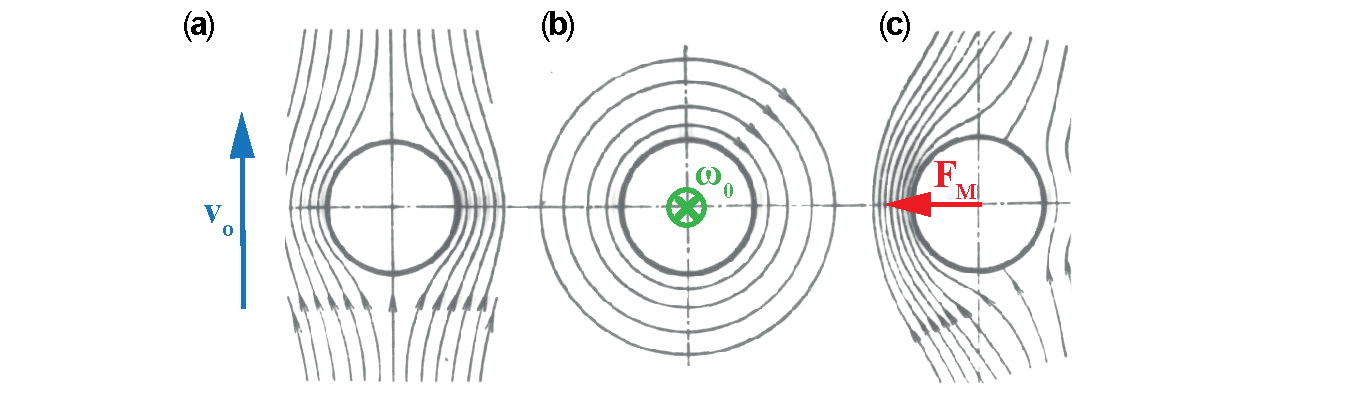
\includegraphics[width=\textwidth]{MagnusEffekt01.pdf}
    \caption[Laminare Str�mung um einen rotierenden Zylinder.]
    {Laminare Str�mung um einen rotierenden Zylinder. \fa Nichtrotierender Zylinder \fb Str�mung in der Grenzschicht \fc �berlagerung.}
    \label{abb:kontmech_magnus01}
\end{figure}

Wir wollen zun�chst eine einfache Plausibilit�tsableitung der Magnus-Kraft machen, bevor wir diese aus der \NVS{} herleiten.
Wir betrachten dabei einen unendlich ausgedehnten Zylinder der L�nge L ($L \gg R$), der sich in einer Str�mumg mit der Geschwindigkeit $\vec{v}_0$ befindet und mit einer Winkelgeschwindigkeit $\vec{\omega}_0$ rotiert.
Die resultierenden Relativgeschwindigkeiten der Fluidstr�mung bez�glich des rotierenden Zylinders ergeben sich dann nach \figref{kontmech_magnus01}\,c folgenderma�en:
\begin{align}
\begin{split}
  \text{linke Seite}:~~~ &\vec{v}_\text{L} = \vec{v}_0 + \vec{\omega}_0 \times \vec{r}~~~~\text{\bzw}\\
  \text{rechte Seite}:~~~&\vec{v}_\text{R} = \vec{v}_0 - \vec{\omega}_0 \times \vec{r}\,.
\end{split}  \label{eq:kontmech_magnus01}
\end{align}

�ber die Bernoulli-Gleichung erhalten wir die Druckdifferenz zwischen beiden Seiten:
\begin{align}
\begin{split}
\Delta p  &= p_\text{R}-p_\text{L} = \frac{\varrho}{2} \lk \vec{v}_\text{L}{}^2 -\vec{v}_\text{R}{}^2 \rk = 2\,\varrho\,\vec{r} \cdot \lk \vec{v}_0  \times \vec{\omega}_0 \rk \,.
\end{split}  \label{eq:kontmech_magnus02}
\end{align}
Daraus ergibt sich eine differentielle Kraft auf ein Oberfl�chenelement nach \figref{kontmech_magnus02} zu:
\begin{align}
\D \vec{F}_\text{M}  &=  2\,\varrho\,\lek \vec{r} \cdot \lk \vec{v}_0  \times \vec{\omega}_0 \rk \rek\, \D \vec{A}\,.
\label{eq:kontmech_magnus02a}
\end{align}
Das differentielle Oberfl�chenelement ist gegeben durch $\D \vec{A} = \vec{r} L\,\D \theta$, wobei wir bereits �ber die Zylinderl�nge $L$ integriert haben.
\begin{align}
\begin{split}
 \D \vec{F}_\text{M}  &=  2\,\varrho\,L \lek R \left| \vec{v}_0  \times \vec{\omega}_0 \right| \cos\theta \rek  \vec{r}\, \D \theta\,.
\end{split}  \label{eq:kontmech_magnus03}
\end{align}

\begin{figure}
    \centering
    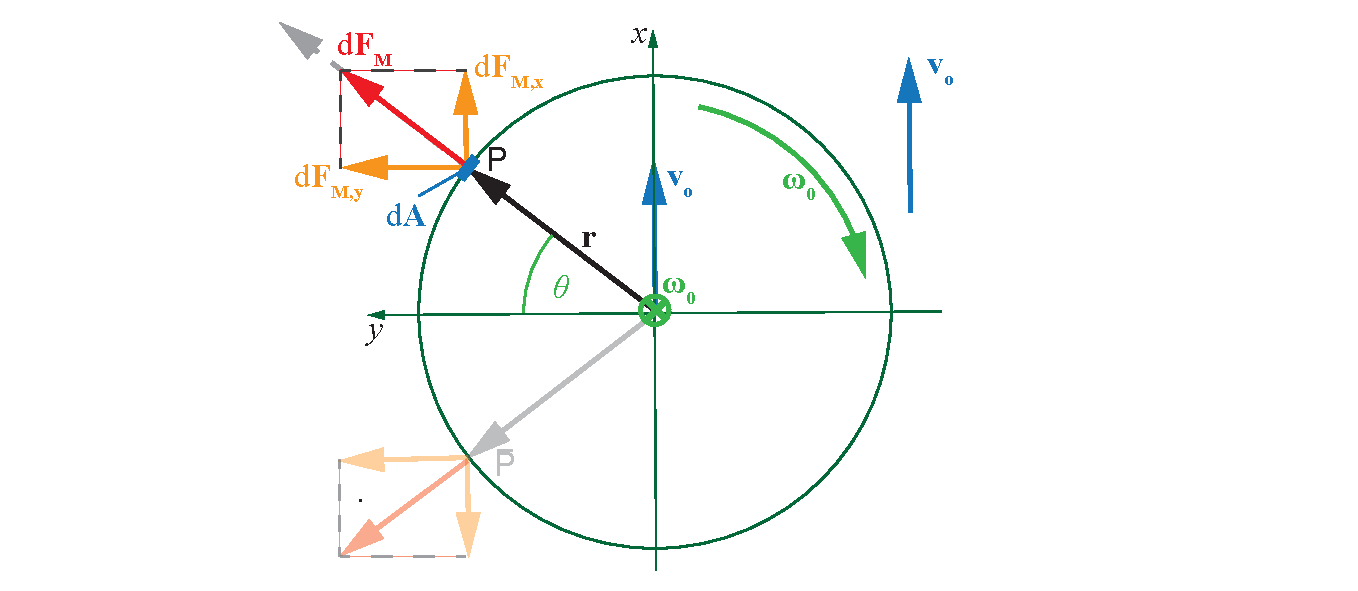
\includegraphics[width=\textwidth]{MagnusEffekt02.pdf}
    \caption[Kraftwirkung auf einen umstr�mten Kreiszylinder.]
    {Kraftwirkung auf einen umstr�mten Kreiszylinder.}
    \label{abb:kontmech_magnus02}
\end{figure}

Das Kraftelement $\D \vec{F}_\text{M}$ wirkt somit in Richtung des Radiusvektors. Wir nutzen jetzt die Symmetrie aus und sehen, dass wir jeweils einen zu $\mathrm{P}$ symmetrischen Punkt $\bar{\mathrm{P}}$ finden, der die gleiche $\D F_{\text{M},y}$-Komponente des Kraftelements hat, deren $\D F_{\text{M},x}$-Komponenten sich aber kompensieren, so dass wir die Integration �ber die gesamte Oberfl�che vereinfachen k�nnen zu:
\begin{align}
\begin{split}
 \vec{F}_\text{M}  & = 4\, \varrho\,L\,R^2\,\left|\vec{v}_0  \times \vec{\omega}_0 \right| \int\limits_{0}^{\pi} \cos^2\theta \,\,\D \theta \, \veceY  = 4\, \varrho\,L\,R^2\,\left|\vec{v}_0  \times \vec{\omega}_0 \right| \,\frac{\pi}2{} \, \veceY \\
                   & = 2\,\pi\,\varrho\,L\,R^2\,\left|\vec{v}_0  \times \vec{\omega}_0 \right| \, \veceY = 2\,\pi\,\varrho\,L\,R^2\, \lk \vec{v}_0  \times \vec{\omega}_0 \rk  \,
\end{split}  \label{eq:kontmech_magnus04}
\end{align}

Auf den Kreiszylinder wirkt also eine senkrecht zur Str�mung gerichtete Kraft, die durch die Zylinderrotation verursacht wird. Dieses Ergebnis findet Anwendung bei Flettner-Rotoren (Rotor-Segelschiffe).\\
Bei optimalen Windverh�ltnissen von \ca $\SI{20}{\metre\per\second}$ quer bis leicht von hinten zur Fahrtrichtung kann der Rotor eine Leistung von etwa 2 MW und mehr erbringen, wobei er mit bis zu 180 Umdrehungen pro Minute rotiert. Die erzeugte Leistung �bersteigt damit die verbrauchte elektrische Leistung von 50 kW des Elektromotors, der das ca 30 Meter hohe Rotorsegel antreibt, um ein Vielfaches. (Siehe \mscr{} \mlkontmechref{FlettnerRotoren.m}.)

Mit dem behandelten Problem des umstr�mten Kreiszylinders haben wir auch den Weg zur Beherrschung des Problems einer umstr�mten Flugzeugtragfl�che bereitet, deren Profil durch eine Abbildung aus dem Kreiszylinderprofil gewonnen werden kann. Bei einer exakten Behandlung eines Flugzeugfl�gels muss man nat�rlich die endliche L�nge des Tragfl�gels ber�cksichtigen, was eine deutliche komplexere 3-dimensionale Aufgabenstellung darstellt.\\
Der Magnus-Effekt spielt auch eine gro�e Rolle bei vielen Ballspielen (Fu�ball, Golf). Hier muss bei der mathematisch-physikalischen Behandlung ebenfalls die endliche Ausdehnung des Ball \bzw der Kugel ber�cksichtigt werden. 
Ebenso sei daraufhin gewiesen, dass wir bei der Herleitung von einer laminaren Str�mung ausgegangen sind, \dh die Betrachtungen gelten nur f�r kleine Reynolds-Zahlen. Bei gr��eren Reynolds-Zahlen treten Verwirbelungen auf, die zu zus�tzlichen Effekten f�hren. Wir werden uns mit solchen Effekten bei der Behandlung des Fliegens als auch bei Untersuchungn zum Ballsport im Band III dieser Reihe intensiver besch�ftigen und dort auch eine allgemeinere Ableitung f�r die Berechnung des Magnus-Effekts geben.

\end{sol} 
\textcolor{blue} {$\rightarrow$ zur} \probref{kontmech_magnus}.\\
\noindent\rule[1ex]{\textwidth}{0.5pt}  \newpage  \clearpage

%-----------------------------------------------------------------------------------------------------------

\begin{sol}{prob:kontmech_SchiffKanal}\label{lsg:kontmech_SchiffKanal} %�bung6
\textbf{Kr�fte auf ein Schiff in einem Kanal}\\ \\

Da Wasser in guter N�herung inkompressibel ist und der Fluss f�r jedes
Zeitintervall $\D t$ an allen Stellen des Schiffes konstant sein muss, k�nnen
wir die Flie�geschwindigkeit aus der verf�gbaren Querschnittsfl�che berechnen.
Die Flie�geschwindigkeit an der Stelle $x$ entlang des Schiffs verh�lt sich
also mit der dort verf�gbaren Fl�che
\begin{align}
  \varrho_\mathrm{W} v(x_1) A(x_1) &= \varrho_\mathrm{W} v(x_2) A(x_2) \notag \\
  \frac{v(x_2)}{v(x_1)} &= \frac{A(x_1)}{A(x_2)} \; , \notag \\
  \frac{v(x)}{v(0)} &= \frac{A(0)}{A(x_2)} \; , \notag \\
  v(x) &= v(0) \, \frac{A(0)}{A(x_2)} \; .
         \label{eq:kontmech_SchiffGeschwindigkeiten}
\end{align}
Als Bezugspunkt nehmen wir das Wasser direkt vor dem Bug des Schiffs. Dort
haben wir (von oben gesehen) auf der linken Seite (vgl.
\figref{kontmech_SchiffKanalAbmessungen}) die Fl�che
\begin{subequations}
  \begin{align}
    A_\mathrm{l}(0) &= a_1 (c_1+c_2) \label{eq:kontmech_SchiffFlaeche1} \\
    \intertext{und auf der rechten Seite}
    A_\mathrm{r}(0) &= a_2 (c_1+c_2) \label{eq:kontmech_SchiffFlaeche2}
  \end{align}
\end{subequations}

Die Querschnittsfl�che, durch die das Wasser str�men kann, h�ngt vom Abstand
$d$ zwischen der Schiffswand und der Wand des Kanals ab. Der Abstand $d$ ist
selbst wieder vom Abstand $x$ vom Bug und der H�he $z$ �ber dem Kiel abh�ngig.
Betrachten wir zun�chst die (von oben gesehen) linke Seite und dort die
Koordinate $y$, so finden wir anhand von
\figref{kontmech_SchiffKanalAbmessungen}
\begin{equation*}
  d_\mathrm{l}(x,z) = a_1 - \frac{B(x,z)}{2} \; .
\end{equation*}
Die von der H�he �ber dem Kliel und der Entfernung vom Bug abh�ngige Breite
$B(x,z)$ des Schiffs ergibt sich nach der Abbildung zu
\begin{equation*}
  B(x,z) = \begin{cases}
    \frac{B(x)}{c_2} \, z & \text{f�r } z < c_2 \; , \\
    B(x) & \text{f�r } c_2 < z \le c_1 + c_2 \; , \\
  \end{cases}
\end{equation*}
wobei im oberen Teil des Schiffes, wo es seine maximale Breite erreicht, gilt
\begin{equation*}
  B(x) = \begin{cases}
    \frac{b}{l_2}\, x & \text{f�r } x \le l_2 \; , \\
    b & \text{f�r } l_2 < x  \le l_1 + l_2 \; .
  \end{cases} 
\end{equation*}

Insgesamt erh�lt man
\begin{equation*}
  B(x,z) = \begin{cases}
    \frac{b}{l_2\,c_2}\, x \, z & \text{f�r } x \le l_2
    \text{ und } z < c_2 \; , \\
    \frac{b}{l_2}\, x  & \text{f�r } x \le l_2 \text{ und }
    c_2 < z \le c_1 + c_2 \; , \\
    \frac{b}{c_2}\, z  & \text{f�r } l_2 < x  \le l_1 + l_2
    \text{ und } z < c_2 \; , \\
    b & \text{f�r } l_2 < x  \le l_1 + l_2 \text{ und } c_2 < z \le c_1
    + c_2 \; .
  \end{cases} 
\end{equation*}
und damit auf der linken Seite
\begin{equation*}
  d_\mathrm{l}(x,z) = \begin{cases}
    a_1 - \frac{b}{2\,l_2\,c_2}\, x \, z & \text{f�r } x \le l_2
    \text{ und } z < c_2 \; , \\
    a_1 - \frac{b}{2\,l_2}\, x  & \text{f�r } x \le l_2 \text{ und }
    c_2 < z \le c_1 + c_2 \; , \\
    a_1 - \frac{b}{2\,c_2}\, z  & \text{f�r } l_2 < x  \le l_1 + l_2
    \text{ und } z < c_2 \; , \\
    a_1 - \frac{b}{2} & \text{f�r } l_2 < x  \le l_1 + l_2
    \text{ und } c_2 < z \le c_1 + c_2 \; .
  \end{cases} 
\end{equation*}
sowie analog auf der rechten Seite  
\begin{equation*}
  d_\mathrm{r}(x,z) = \begin{cases}
    a_2 - \frac{b}{2\,l_2\,c_2}\, x \, z & \text{f�r } x \le l_2 \text{ und }
    z < c_2 \; , \\
    a_2 - \frac{b}{2\,l_2}\, x  & \text{f�r } x \le l_2 \text{ und }
    c_2 < z \le c_1 + c_2 \; , \\
    a_2 - \frac{b}{2\,c_2}\, z  & \text{f�r } l_2 < x  \le l_1 + l_2
    \text{ und } z < c_2 \; , \\
    a_2 - \frac{b}{2} & \text{f�r } l_2 < x  \le l_1 + l_2 \text{ und }
    c_2 < z \le c_1 + c_2 \; .
  \end{cases} 
\end{equation*}

Dies k�nnen wir nun nutzen, um die Querschnittsfl�che zu berechnen. Wir
erhalten f�r $x < l_2$
\begin{multline*}
  A_\mathrm{l}(x) = \int_{0}^{c_1 + c_2} d_\mathrm{l}(x,z) \, \D z
  = \int_{0}^{c_2} \lk a_1 - \frac{b}{2\,l_2\,c_2}\, x \, z \rk \D z
  + \int_{c_2}^{c_1 + c_2}  \lk a_1 - \frac{b}{2\,l_2}\, x \rk \D z \\
  = a_1 \, c_2 -  \frac{b\,c_2}{4\,l_2} \, x
  + \lk a_1 - \frac{b}{2\,l_2}\, x \rk c_1
  = a_1 \lk c_1 + c_2 \rk - \frac{b \lk 2 c_1 + c_2 \rk}{4\,l_2} \, x 
\end{multline*}
und im Fall $l_2 < x \le l_1 + l_2$
\begin{multline*}
  A_\mathrm{l} = \int_{0}^{c_1 + c_2} d_\mathrm{l}(x,z) \, \D z
  = \int_{0}^{c_2} \lk a_1 - \frac{b}{2\,c_2}\, z \rk \D z
  + \int_{c_2}^{c_1 + c_2}  \lk a_1 - \frac{b}{2} \rk \D z \\
  = a_1 \, c_2 -  \frac{b\,c_2}{4} 
  + \lk a_1 - \frac{b}{2} \rk c_1
  = a_1 \lk c_1 + c_2 \rk - \frac{b \lk 2 c_1 + c_2 \rk}{4} 
\end{multline*}
Dies l�sst sich zusammenfassen zu
\begin{equation*}
  A_\mathrm{l}(x) = \begin{cases}
    a_1 \lk c_1 + c_2 \rk - \frac{b \lk 2 c_1 + c_2 \rk}{4\,l_2} \, x
    & \text{f�r } x < l_2 \; , \\
    a_1 \lk c_1 + c_2 \rk - \frac{b \lk 2 c_1 + c_2 \rk}{4}
    & \text{f�r } l_2 < x \le l_1 + l_2 \; .
  \end{cases}
\end{equation*}
und f�r die rechte Seite vollkommen analog berechnen zu
\begin{equation*}
  A_\mathrm{r}(x) = \begin{cases}
    a_2 \lk c_1 + c_2 \rk - \frac{b \lk 2 c_1 + c_2 \rk}{4\,l_2} \, x
    & \text{f�r } x < l_2 \; , \\
    a_2 \lk c_1 + c_2 \rk - \frac{b \lk 2 c_1 + c_2 \rk}{4}
    & \text{f�r } l_2 < x \le l_1 + l_2 \; .
  \end{cases}
\end{equation*}

Die bisher durchgef�hrten Zwischenrechnungen erm�glichen uns nun, die
Flie�gechwindigkeit des Wassers relativ zum Schiff abh�ngig vom Ort $x$
zu bestimmen. Zusammen mit \eqref{eq:kontmech_SchiffGeschwindigkeiten},
den Fl�chen $A_\mathrm{l}(0)$ und $A_\mathrm{r}(0)$ aus den Gleichungen
\eqref{eq:kontmech_SchiffFlaeche1} und \eqref{eq:kontmech_SchiffFlaeche1}
sowie $v(0) = v_0$ erhalten wir
\begin{align}
  v_\mathrm{l}(x) &= \begin{cases} v_0 \, \frac{a_1 \lk c_1 + c_2 \rk}{a_1
      \lk c_1 + c_2 \rk - \frac{b \lk 2 c_1 + c_2 \rk}{4\,l_2} \, x}
    & \text{f�r } x < l_2 \; , \\
    v_0 \, \frac{a_1 \lk c_1 + c_2 \rk}{a_1 \lk c_1 + c_2 \rk - \frac{b
        \lk 2 c_1 + c_2 \rk}{4}}
    & \text{f�r } l_2 < x \le l_1 + l_2 
  \end{cases} \\
  \intertext{und}
  v_\mathrm{r}(x) &= \begin{cases} v_0 \, \frac{a_2 \lk c_1 + c_2 \rk}{a_2
      \lk c_1 + c_2 \rk - \frac{b \lk 2 c_1 + c_2 \rk}{4\,l_2} \, x}
    & \text{f�r } x < l_2 \; , \\
    v_0 \, \frac{a_2 \lk c_1 + c_2 \rk}{a_2 \lk c_1 + c_2 \rk - \frac{b
        \lk 2 c_1 + c_2 \rk}{4}}
    & \text{f�r } l_2 < x \le l_1 + l_2 \; . 
  \end{cases} 
\end{align}

Sei $p_0$ der Druck im Wasser, das relativ zum Schiff die Flie�geschwindigkeit
$v_0$ habe. Dann l�sst sich mit der Bernoulli-Gleichung
\eqref{eq:kontmech_BernoulliGl} der Druck auf die Seitenw�nde des Schiffs
ermitteln. Wir finden auf der linken Seite
\begin{equation*}
  \frac{1}{2} \varrho \, v_l(x)^2 + p_l(x) = \frac{1}{2} \varrho \, v_0^2 + p_0
\end{equation*}
oder 
\begin{align*}
  p_l(x) &= p_0 + \frac{1}{2} \varrho \lk v_0^2 -  v_l(x)^2 \rk \\
         &= p_0 + \frac{1}{2} \varrho v_0^2 \begin{cases}
           1 - \lk \frac{a_1 \lk c_1 + c_2 \rk}{a_1\lk c_1 + c_2 \rk
             - \frac{b \lk 2 c_1 + c_2 \rk}{4\,l_2} \, x} \rk^2 
           & \text{f�r } x < l_2 \; , \\
         1 - \lk \frac{a_1 \lk c_1 + c_2 \rk}{a_1 \lk c_1 + c_2 \rk - \frac{b
             \lk 2 c_1 + c_2 \rk}{4}} \rk^2
         & \text{f�r } l_2 < x \le l_1 + l_2 \; .
         \end{cases}
\end{align*}
Analog findet man auf der rechten Seite
\begin{align*}
  p_r(x) &= p_0 + \frac{1}{2} \varrho \lk v_0^2 -  v_r(x)^2 \rk \\
         &= p_0 + \frac{1}{2} \varrho v_0^2 \begin{cases}
           1 - \lk \frac{a_2 \lk c_1 + c_2 \rk}{a_2\lk c_1 + c_2 \rk
             - \frac{b \lk 2 c_1 + c_2 \rk}{4\,l_2} \, x} \rk^2 
           & \text{f�r } x < l_2 \; , \\
         1 - \lk \frac{a_2 \lk c_1 + c_2 \rk}{a_2 \lk c_1 + c_2 \rk - \frac{b
             \lk 2 c_1 + c_2 \rk}{4}} \rk^2
         & \text{f�r } l_2 < x \le l_1 + l_2 \; .
         \end{cases}
\end{align*}
F�r die resultierende Kraft und das resultierende Moment auf das Schiff
reicht es, in den folgenden Schritten aufgrund der Symmetrie des Schiffs
von der Druckdifferenz auf beiden Seiten auszugehen. Nach
\figref{kontmech_SchiffKanalAbmessungen} erwarten wir einen gr��eren
Druck auf der linken Seite, da dort die Querschnittsfl�che gr��er und somit
die Flie�geschwindigkeit kleiner ist, und somit eine effektive Kraftwirkung
nach rechts. Diese wird von der Durckdifferenz
\begin{align}
  \Delta p &= p_l(x) - p_r(x) \\
           &= \frac{1}{2} \varrho v_0^2 \begin{cases}
             \lk \frac{a_1 \lk c_1 + c_2 \rk}{a_1\lk c_1 + c_2 \rk
               - \frac{b \lk 2 c_1 + c_2 \rk}{4\,l_2} \, x} \rk^2
             - \lk \frac{a_2 \lk c_1 + c_2 \rk}{a_2\lk c_1 + c_2 \rk
               - \frac{b \lk 2 c_1 + c_2 \rk}{4\,l_2} \, x} \rk^2 
             & \text{f�r } x < l_2 \; , \\
             \lk \frac{a_1 \lk c_1 + c_2 \rk}{a_1 \lk c_1 + c_2 \rk - \frac{b
                 \lk 2 c_1 + c_2 \rk}{4}} \rk^2
             - \lk \frac{a_2 \lk c_1 + c_2 \rk}{a_2 \lk c_1 + c_2 \rk - \frac{b
                 \lk 2 c_1 + c_2 \rk}{4}} \rk^2
             & \text{f�r } l_2 < x \le l_1 + l_2
           \end{cases}
               \label{eq:kontmech_SchiffKanalDruckdiff}
\end{align}
bewirkt.

Die Kraft und das Drehmoment sollen auf den Schwerpunkt des Schiffes bezogen
werden. Da wir uns nur an der Bewegung in der $x$-$y$-Ebene interessiert
sind, ben�tigen wir auch den Schwerpunkt nur in dieser. Aus Symmeriegr�nden
erkennt man sofort, dass $y_\mathrm{S} = 0$. F�r die $x$-Koordinate m�ssen
wir jedoch die Form des Bugs ber�cksichtigen. Wir berechnen unter
Ber�cksichtigung der homegenen Massendichte
\begin{subequations}
  \allowdisplaybreaks
  \begin{multline}
    x_\mathrm{S} = \frac{1}{V} \int_{0}^{l_1+l_2}\D x \, \int_{0}^{c_1+c_2} \D z \,
    \int_{-B(x,z)/2}^{B(x,z)/2} \D y \, x
    = \frac{1}{V} \int_{0}^{l_1+l_2}\D x \, \int_{0}^{c_1+c_2} \D z \, x \,
    B(x,z) \\
    = \frac{1}{V} \int_{0}^{l_1+l_2}\D x \left \{ \int_{0}^{c_2} \D z \, x \,
      \frac{B(x)}{c_2} \, z + \int_{c_2}^{c_1 + c_2} \D z \, x \, B(x) \right \}
    = \frac{1}{V} \int_{0}^{l_1+l_2}\D x \left \{ x \, \frac{c_2}{2} \, B(x)
      + x \, c_1 \, B(x) \right \} \\
    = \frac{1}{V} \int_{0}^{l_1+l_2}\D x \, x \lk \frac{c_2}{2} +c_1 \rk B(x)
    = \frac{1}{V} \lk \frac{c_2}{2} +c_1 \rk  \left \{ \int_{0}^{l_2}\D x
      \, \frac{b}{l_2}\, x^2 +  \int_{l_2}^{l_1 + l_2}\D x \, b \, x
    \right \} \\
    = \frac{1}{V} \lk \frac{c_2}{2} +c_1 \rk  \left \{ \frac{b\,l_2^2}{3}
      + \frac{b\,\lk l_1 + l_2 \rk^2}{2} - \frac{b\, l_2^2}{2}\right \}
    = \frac{1}{V} \lk \frac{c_2}{2} +c_1 \rk  b \left \{ \frac{\lk l_1 + l_2
        \rk^2}{2} - \frac{l_2^2}{6} \right \}
    \label{eq:kontmech_SchiffSchwerpunkt1}
  \end{multline}
  Mit dem Volumen des Schiffs
  \begin{multline}
    V = \int_{0}^{l_1+l_2}\D x \, \int_{0}^{c_1+c_2} \D z \,
    \int_{-B(x,z)/2}^{B(x,z)/2} \D y 
    = \int_{0}^{l_1+l_2}\D x \lk \frac{c_2}{2} +c_1 \rk B(x) \\
    = \lk \frac{c_2}{2} +c_1 \rk  \left \{ \int_{0}^{l_2}\D x
      \, \frac{b}{l_2}\, x +  \int_{l_2}^{l_1 + l_2}\D x \, b \right \} 
    = \lk \frac{c_2}{2} +c_1 \rk  \left \{ \frac{b\,l_2}{2}
      + b\,\lk l_1 + l_2 \rk - b\, l_2 \right \}
    = \lk \frac{c_2}{2} +c_1 \rk  b \lk l_1 + \frac{l_2}{2} \rk
    \label{eq:kontmech_SchiffVolumen}
  \end{multline}
  f�hrt das schlie�lich auf
  \begin{equation}
    x_\mathrm{S} = \frac{\frac{\lk l_1 + l_2 \rk^2}{2} - \frac{l_2^2}{6}}
    {l_1 + \frac{l_2}{2}} = \frac{3 \lk l_1 + l_2 \rk^2 - l_2^2}
    {6 \, l_1 + 3 \, l_2}
    = \frac{3 l_1^2 + 6 l_1 l_2 +2 l_2^2}{6 \, l_1 + 3 \, l_2}
    \; .
    \label{eq:kontmech_SchiffSchwerpunkt2}
  \end{equation}
\end{subequations}

Wir berechnen zun�chst die Kraft auf den Schwerpunkt. Diese hat zwei
Komponenten. Auf den Bug wirkt ein kleinerer Druck als auf das Heck. Das hat
eine Kraft in negativer $x$-Richtung zur Folge, die uns hier jedoch nicht
interessiert, da sie mit einer Kursabweichung des Schiffst nichts zu tun
hat und in dieser Richtung weitere Komponenten wie der Antrieb oder die
Reibung �berwiegen. Jedoch gibt es auch eine $y$-Komponente. Diese ergibt sich
aus dem Druckunterschied bezogen auf die projizierte Fl�che der Schiffswand
auf die $x$-$z$-Ebene, wobei die projizierte H�he  $c_1 + c_2$ betr�gt. Man
erh�lt
{ \allowdisplaybreaks
  \begin{multline}
    F_y = (c_1+c_2) \int_0^{l_1+ l_2} \Delta p(x)\,\D x \\
    = \frac{1}{2} \varrho v_0^2 \, (c_1+c_2) \int_0^{l_2}
    \left \{ \lk \frac{a_1 \lk c_1 + c_2 \rk}{a_1\lk c_1 + c_2 \rk
        - \frac{b \lk 2 c_1 + c_2 \rk}{4\,l_2} \, x} \rk^2
      - \lk \frac{a_2 \lk c_1 + c_2 \rk}{a_2\lk c_1 + c_2 \rk
        - \frac{b \lk 2 c_1 + c_2 \rk}{4\,l_2} \, x} \rk^2 \right \} \,\D x \\
    + \frac{1}{2} \varrho v_0^2 \, (c_1+c_2) \, l_1 \left \{
      \lk \frac{a_1 \lk c_1 + c_2 \rk}{a_1 \lk c_1 + c_2 \rk - \frac{b
          \lk 2 c_1 + c_2 \rk}{4}} \rk^2
      - \lk \frac{a_2 \lk c_1 + c_2 \rk}{a_2 \lk c_1 + c_2 \rk - \frac{b
          \lk 2 c_1 + c_2 \rk}{4}} \rk^2 \right \}  \\
    = \frac{1}{2} \varrho v_0^2 \, (c_1+c_2) \, \frac{4\,l_2}{b \lk 2 c_1
      + c_2 \rk}
    \left . \left \{ \frac{a_1^2 \lk c_1 + c_2 \rk^2}{a_1\lk c_1 + c_2 \rk
          - \frac{b \lk 2 c_1 + c_2 \rk}{4\,l_2} \, x} 
        - \frac{a_2^2 \lk c_1 + c_2 \rk^2}{a_2\lk c_1 + c_2 \rk
          - \frac{b \lk 2 c_1 + c_2 \rk}{4\,l_2} \, x}  \right \}
    \right |_{0}^{l_2} \\
    + \frac{1}{2} \varrho v_0^2 \, (c_1+c_2) \, l_1 \left \{
      \lk \frac{a_1 \lk c_1 + c_2 \rk}{a_1 \lk c_1 + c_2 \rk - \frac{b
          \lk 2 c_1 + c_2 \rk}{4}} \rk^2
      - \lk \frac{a_2 \lk c_1 + c_2 \rk}{a_2 \lk c_1 + c_2 \rk - \frac{b
          \lk 2 c_1 + c_2 \rk}{4}} \rk^2 \right \}  \\
    = \frac{1}{2} \varrho v_0^2 \, \frac{4\,l_2\lk c_1 + c_2\rk}{b\lk 2c_1
      + c_2 \rk}
    \Bigg \{ \frac{a_1^2 \lk c_1 + c_2 \rk^2}{a_1\lk c_1 + c_2 \rk
      - \frac{b \lk 2 c_1 + c_2 \rk}{4}}
    - a_1 \lk c_1 + c_2 \rk 
    - \frac{a_2^2 \lk c_1 + c_2 \rk^2}{a_2\lk c_1 + c_2 \rk
      - \frac{b \lk 2 c_1 + c_2 \rk}{4}} 
    + a_2 \, \lk c_1 + c_2 \rk  \Bigg \} \\
    + \frac{1}{2} \varrho v_0^2 \, (c_1+c_2) \, l_1 \left \{
      \lk \frac{a_1 \lk c_1 + c_2 \rk}{a_1 \lk c_1 + c_2 \rk - \frac{b
          \lk 2 c_1 + c_2 \rk}{4}} \rk^2
      - \lk \frac{a_2 \lk c_1 + c_2 \rk}{a_2 \lk c_1 + c_2 \rk - \frac{b
          \lk 2 c_1 + c_2 \rk}{4}} \rk^2 \right \}  \; . \\
  \end{multline}
}

W�hrend f�r die Kraft schnell einsichtig war, dass die auf die $x$-$z$-Ebene
projizierte Fl�che herangezogen werden kann, um die effektive Kraft zu
berechnen, ist eine �hnliche Vereinfachung f�r das Drehmoment nicht so
schnell zu erkennen. Doch auch hier k�nnen wir einen recht einfachen Ausdruck
finden, der sich auf die Druckdifferenz zur�ckf�hren l�sst. Um das zu erkennen
betrachten wir \figref{kontmech_SchiffKanalKraefte}.

\begin{figure}
  \centering
  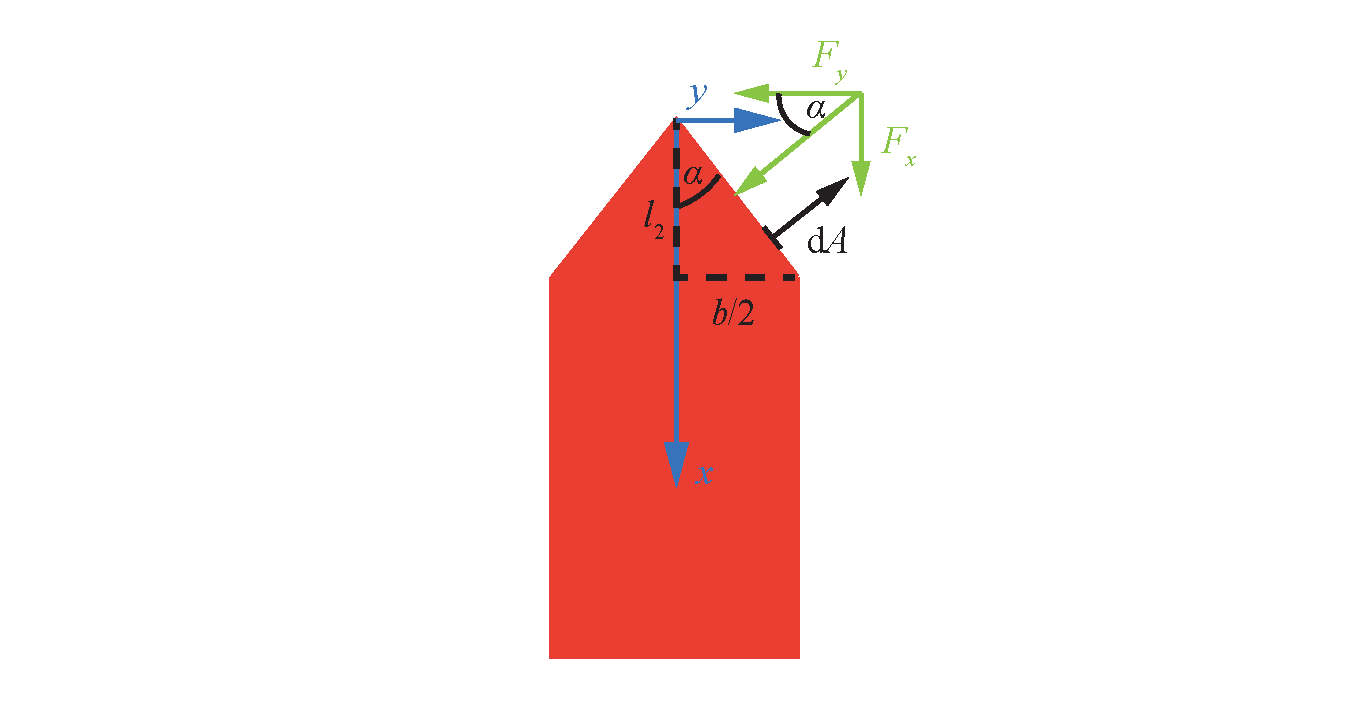
\includegraphics[width=\textwidth]{SchiffKanalKraefte}
  \caption[Kr�fte auf ein Schiff im Kanal]
  {Kr�fte auf eine Schiff im Kanal, wie sie durch den Wasserdruck
    verursacht werden.}
  \label{abb:kontmech_SchiffKanalKraefte}
\end{figure}

Da wir nur an Drehungen um die $z$-Achse interessiert sind, m�ssen wir
keine Kraftkomponenten in $z$-Richtung beachten, denn diese k�nnten kein
solches Drehmoment bewirken. In jeder H�he interessieren wir uns also nur
vom Abstand des Angriffspunkts einer Kraft von der $z$-Achse um den
Schwerpunkt, den wir entsprechend auf der linken und rechten Seite des
Bugs mit 
\begin{equation}
  \vec{r}_r = \begin{pmatrix} x-x_\mathrm{S} \\ y \\ 0 \end{pmatrix} \; , \qquad
  \vec{r}_l = \begin{pmatrix} x-x_\mathrm{S} \\ -y \\ 0 \end{pmatrix} 
\end{equation}
angeben k�nnen. F�r Kr�fte, die auf beiden Seiten jeweils auf das
Fl�chenelement $\D A$ wirken, finden wir
\begin{equation}
  \D \vec{F}_r = \begin{pmatrix} p_r \,\D A\, \sin\alpha \\
    -p_r \, \D A \, \cos\alpha \\ 0 \end{pmatrix} \; , \qquad
  \D \vec{F}_l = \begin{pmatrix} p_l \,\D A\, \sin\alpha \\
    p_l \, \D A \, \cos\alpha \\ 0 \end{pmatrix} \; .
\end{equation}
Um unteren schr�gen Teil des Rumpfes wirkt die Kraft durch den Druck
nat�rlich nicht nur in der $x$-$y$-Ebene. Da wir sp�ter jedoch wieder
�ber die H�he $c_1$ integrieren, um das gesamte Drehmoment zu erhalten,
und nicht �ber die schr�ge Fl�che ber�cksichtigen wir automatisch nur
die relevante Kraftkomponente. Die $z$-Komponente der Kraft ist, wie oben
beschrieben, f�r uns nicht relevant und wird hier zur �bersichtlichkeit
in der Rechnung nicht angegeben.

Das Drehmoment berechnet sich dann zu
\begin{equation}
  \D \vec{M} = \vec{r}_r \times \vec{F}_r + \vec{r}_l \times \vec{F}_l 
  = \begin{pmatrix} x-x_\mathrm{S} \\ y \\ 0 \end{pmatrix}
  \times \begin{pmatrix} p_r \,\D A\, \sin\alpha \\
    -p_r \, \D A \, \cos\alpha \\ 0 \end{pmatrix}
  + \begin{pmatrix} x-x_\mathrm{S} \\ -y \\ 0 \end{pmatrix}
  \times \begin{pmatrix} p_l \,\D A\, \sin\alpha \\
    p_l \, \D A \, \cos\alpha \\ 0 \end{pmatrix}
\end{equation}
mit der f�r uns relevanten $z$-Komponente
\begin{multline}
  \D M_z = - (x-x_\mathrm{S}) p_r \, \D A\, \cos\alpha - y\, p_r \, \D A \,
  \sin\alpha
  + (x-x_\mathrm{S}) p_l \, \D A\, \cos\alpha - y\, p_l \, \D A \, \sin\alpha \\
  = -(x \, \cos\alpha + y\, \sin\alpha) p_r \,\D A + x_\mathrm{S} \, \cos\alpha
  \, p_r \, \D A 
  + (x \, \cos\alpha + y\, \sin\alpha) p_l \,\D A - x_\mathrm{S} \, \cos\alpha
  \, p_l \, \D A \\
  = (x \, \cos\alpha + y\, \sin\alpha) \Delta p(x) \,\D A
  - x_\mathrm{S} \, \cos\alpha \, \Delta p(x) \, \D A \; .
\end{multline}
Hier erkennen wir bereits, dass erneut nur die Druckdifferenz entscheidend
ist. Die Ausdr�cke lassen sich jedoch weiter vereinfachen. Wir ber�cksichtigen,
dass nach \figref{kontmech_SchiffKanalKraefte}
\begin{equation}
  \tan \alpha = \frac{y}{x} \qquad \text{bzw.} \qquad
  y(x) = \tan\alpha\, x \; .
\end{equation}
Damit erhalten wir
\begin{equation}
  \D M_z = \lk x \, \cos\alpha + x\, \frac{\sin^2\alpha}{\cos\alpha} \rk
  \Delta p(x) \,\D A - x_\mathrm{S} \, \cos\alpha \, \Delta p(x) \, \D A 
  = \frac{x}{\cos\alpha}\, \Delta p(x) \,\D A
  - x_\mathrm{S} \, \cos\alpha \, \Delta p(x) \, \D A \; .
\end{equation}
Wenn wir nun noch nach \figref{kontmech_SchiffKanalKraefte} ber�cksichtigen,
dass
\begin{equation}
  \D A = \lk c_1 + c_2 \rk \frac{\D x}{\cos\alpha} \; ,
\end{equation}
dann f�hrt das auf
\begin{equation}
  \D M_z = \frac{x}{\cos^2\alpha}\, \Delta p(x) \, \lk c_1 + c_2 \rk \, \D x
  - x_\mathrm{S} \, \Delta p(x) \, \lk c_1 + c_2 \rk \, \D x \; .
\end{equation}
Schlie�lich dr�cken wir den Winkel $\alpha$ durch bekannte Ma�e des Schiffs
aus,
\begin{equation*}
  \cos \alpha = \frac{l_2}{\sqrt{l_2^2 + (b/2)^2}} \;, \qquad \text{also}
  \qquad \frac{1}{\cos^2\alpha} = \frac{l_2^2 + b^2/4}{l_2^2}
  = 1 + \frac{b^2}{4 l_2^2} \; ,
\end{equation*}
und erhalten daraus
\begin{equation}
  \D M_z = x \, \Delta p(x) \, \lk 1 + \frac{b^2}{4 l_2^2} \rk 
  \lk c_1 + c_2 \rk \, \D x
  - x_\mathrm{S} \, \Delta p(x) \, \lk c_1 + c_2 \rk \, \D x \; .
\end{equation}

F�r den Anteil des Bugs erhalten wir damit
{
  \allowdisplaybreaks
  \begin{multline}
    \lk M_1 \rk_z = \int_0^{l_2} \D M_z
    = \lk 1 + \frac{b^2}{4 l_2^2} \rk \lk c_1 + c_2 \rk  \int_0^{l_2} x \,
    \Delta p(x) \, \D x
    - x_\mathrm{S} \, \lk c_1 + c_2 \rk \, \int_0^{l_2} \Delta p(x) \, \D x \\
    % 
    = \frac{1}{2} \varrho v_0^2 \, \lk 1 + \frac{b^2}{4 l_2^2} \rk \lk c_1
    + c_2 \rk  \int_0^{l_2} x \, \left \{ \lk \frac{a_1 \lk c_1 + c_2 \rk}
      {a_1\lk c_1 + c_2 \rk - \frac{b \lk 2 c_1 + c_2 \rk}{4\,l_2} \, x} \rk^2
      - \lk \frac{a_2 \lk c_1 + c_2 \rk}{a_2\lk c_1 + c_2 \rk
        - \frac{b \lk 2 c_1 + c_2 \rk}{4\,l_2} \, x} \rk^2 \right \} \, \D x \\
    - \frac{1}{2} \varrho v_0^2 \, x_\mathrm{S} \lk c_1 + c_2 \rk \, \int_0^{l_2}
    \left \{ \lk \frac{a_1 \lk c_1 + c_2 \rk}{a_1\lk c_1 + c_2 \rk
        - \frac{b \lk 2 c_1 + c_2 \rk}{4\,l_2} \, x} \rk^2
      - \lk \frac{a_2 \lk c_1 + c_2 \rk}{a_2\lk c_1 + c_2 \rk
        - \frac{b \lk 2 c_1 + c_2 \rk}{4\,l_2} \, x} \rk^2 \right \} \,\D x \\
    % 
    = \frac{1}{2} \varrho v_0^2 \, \lk 1 + \frac{b^2}{4 l_2^2} \rk \lk c_1
    + c_2 \rk \, \frac{4\,l_2}{b \lk 2 c_1 + c_2 \rk}
    \left . x \, \left \{ \frac{a_1^2 \lk c_1 + c_2 \rk^2}{a_1\lk c_1 + c_2 \rk
          - \frac{b \lk 2 c_1 + c_2 \rk}{4\,l_2} \, x} 
        - \frac{a_2^2 \lk c_1 + c_2 \rk^2}{a_2\lk c_1 + c_2 \rk
          - \frac{b \lk 2 c_1 + c_2 \rk}{4\,l_2} \, x}  \right \}
    \right |_{0}^{l_2} \\
 - \frac{1}{2} \varrho v_0^2 \, \lk 1 + \frac{b^2}{4 l_2^2} \rk \lk c_1
    + c_2 \rk \, \frac{4\,l_2}{b \lk 2 c_1 + c_2 \rk} \int_0^{l_2} 
    \left \{ \frac{a_1^2 \lk c_1 + c_2 \rk^2}{a_1\lk c_1 + c_2 \rk
        - \frac{b \lk 2 c_1 + c_2 \rk}{4\,l_2} \, x} 
      - \frac{a_2^2 \lk c_1 + c_2 \rk^2}{a_2\lk c_1 + c_2 \rk
        - \frac{b \lk 2 c_1 + c_2 \rk}{4\,l_2} \, x}  \right \} \, \D x \\
    - \frac{1}{2} \varrho v_0^2 \, x_\mathrm{S} \frac{4\,l_2 \lk c_1 + c_2 \rk}
    {b \lk 2c_1 + c_2 \rk}
    \Bigg \{ \frac{a_1^2 \lk c_1 + c_2 \rk^2}{a_1\lk c_1 + c_2 \rk
      - \frac{b \lk 2 c_1 + c_2 \rk}{4}}
    - a_1 \lk c_1 + c_2 \rk 
    - \frac{a_2^2 \lk c_1 + c_2 \rk^2}{a_2\lk c_1 + c_2 \rk
      - \frac{b \lk 2 c_1 + c_2 \rk}{4}} 
    + a_2 \, \lk c_1 + c_2 \rk  \Bigg \} \\
    % 
    = \frac{1}{2} \varrho v_0^2 \, \lk 1 + \frac{b^2}{4 l_2^2} \rk \,
    \frac{4\,l_2^2 \lk c_1 + c_2 \rk}{b \lk 2 c_1 + c_2 \rk}
    \left \{\frac{a_1^2 \lk c_1 + c_2 \rk^2}{a_1\lk c_1 + c_2 \rk
        - \frac{b \lk 2 c_1 + c_2 \rk}{4}} 
      - \frac{a_2^2 \lk c_1 + c_2 \rk^2}{a_2\lk c_1 + c_2 \rk
        - \frac{b \lk 2 c_1 + c_2 \rk}{4}}  \right \} \\
    + \frac{1}{2} \varrho v_0^2 \, \lk 1 + \frac{b^2}{4 l_2^2} \rk \,
    \frac{16\,l_2^2 \lk c_1 + c_2 \rk}{b^2 \lk 2 c_1 + c_2 \rk^2}  
    \Biggl \{ a_1^2 \lk c_1 + c_2 \rk^2 \ln \lk a_1\lk c_1 + c_2 \rk
          - \frac{b \lk 2 c_1 + c_2 \rk}{4\,l_2} \, x \rk \\
        - a_2^2 \lk c_1 + c_2 \rk^2 \ln \lk a_2\lk c_1 + c_2 \rk
          - \frac{b \lk 2 c_1 + c_2 \rk}{4\,l_2} \, x \rk  \Biggr \}
    \Biggr |_{0}^{l_2} \\
    - \frac{1}{2} \varrho v_0^2 \, x_\mathrm{S} \frac{4\,l_2}{b}
    \Bigg \{ \frac{a_1^2 \lk c_1 + c_2 \rk^2}{a_1\lk c_1 + c_2 \rk
      - \frac{b \lk 2 c_1 + c_2 \rk}{4}}
    - a_1 \lk c_1 + c_2 \rk 
    - \frac{a_2^2 \lk c_1 + c_2 \rk^2}{a_2\lk c_1 + c_2 \rk
      - \frac{b \lk 2 c_1 + c_2 \rk}{4}} 
    + a_2 \, \lk c_1 + c_2 \rk  \Bigg \} \\ 
    % 
    = \frac{1}{2} \varrho v_0^2 \, \lk 1 + \frac{b^2}{4 l_2^2} \rk \,
    \frac{4\,l_2^2 \lk c_1 + c_2 \rk}{b \lk 2 c_1 + c_2 \rk}
    \left \{\frac{a_1^2 \lk c_1 + c_2 \rk^2}{a_1\lk c_1 + c_2 \rk
        - \frac{b \lk 2 c_1 + c_2 \rk}{4}} 
      - \frac{a_2^2 \lk c_1 + c_2 \rk^2}{a_2\lk c_1 + c_2 \rk
        - \frac{b \lk 2 c_1 + c_2 \rk}{4}}  \right \} \\
    + \frac{1}{2} \varrho v_0^2 \, \lk 1 + \frac{b^2}{4 l_2^2} \rk \,
    \frac{16\,l_2^2 \lk c_1 + c_2 \rk}{b^2 \lk 2 c_1 + c_2 \rk^2}  
    \Biggl \{ a_1^2 \lk c_1 + c_2 \rk^2 \ln \lk \frac{a_1\lk c_1 + c_2 \rk
          - \frac{b \lk 2 c_1 + c_2 \rk}{4}}{a_1\lk c_1 + c_2 \rk} \rk \\
        - a_2^2 \lk c_1 + c_2 \rk^2 \ln \lk \frac{a_2\lk c_1 + c_2 \rk
          - \frac{b \lk 2 c_1 + c_2 \rk}{4}}{a_2\lk c_1 + c_2 \rk} \rk
        \Biggr \} \\
    - \frac{1}{2} \varrho v_0^2 \, x_\mathrm{S} \frac{4\,l_2}{b}
    \Bigg \{ \frac{a_1^2 \lk c_1 + c_2 \rk^2}{a_1\lk c_1 + c_2 \rk
      - \frac{b \lk 2 c_1 + c_2 \rk}{4}}
    - a_1 \lk c_1 + c_2 \rk 
    - \frac{a_2^2 \lk c_1 + c_2 \rk^2}{a_2\lk c_1 + c_2 \rk
      - \frac{b \lk 2 c_1 + c_2 \rk}{4}} 
    + a_2 \, \lk c_1 + c_2 \rk  \Bigg \} \; .
  \end{multline}
}

F�r den hinteren Teil des Schiffs der L�nge $l_1$ wirkt nur eine Kraft
in $y$-Richtung. Dadurch ergibt sich f�r das Drehmoment
\begin{equation}
  \D \vec{M} = \begin{pmatrix} x-x_\mathrm{S} \\ y \\ 0 \end{pmatrix}
  \times \begin{pmatrix} 0 \\ -p_r \, \D A \\ 0 \end{pmatrix}
  + \begin{pmatrix} x-x_\mathrm{S} \\ -y \\ 0 \end{pmatrix}
  \times \begin{pmatrix} 0 \\  p_l \, \D A \\ 0 \end{pmatrix}
\end{equation}
mit der $z$-Komponente
\begin{equation}
  \D M_z = - (x-x_\mathrm{S}) p_r \, \D A + (x-x_\mathrm{S}) p_l \, \D A 
  = (x-x_\mathrm{S}) \Delta p \, \D A \; .
\end{equation}
Mit
\begin{equation}
  \D A = \lk c_1 + c_2 \rk \D x 
\end{equation}
in diesem geraden Teil des Schiffs ergibt sich
\begin{equation}
  \D M_z = (x-x_\mathrm{S}) \Delta p \, \lk c_1 + c_2 \rk \D x \; .
\end{equation}

Insbesondere beachten wir, dass der Druck hier nicht von $x$ abh�ngt, wie
wir aus \eqref{eq:kontmech_SchiffKanalDruckdiff} wissen. Der entsprechende
Beitrag zum Drehmoment berechnet sich damit zu
{ \allowdisplaybreaks
  \begin{multline}
    \lk M_2 \rk_z = \int_{l_2}^{l_1+l_2} \D M_z
    = \Delta p \, \lk c_1 + c_2 \rk \int_{l_2}^{l_1+l_2} \D M_z (x-x_\mathrm{S})
    \D x 
    = \Delta p \, \lk c_1 + c_2 \rk \left \{ \left . \frac{1}{2} x^2
      \right |_{l_2}^{l_1+l_2} - x_s l_1 \right \} \\
    = \Delta p \, \lk c_1 + c_2 \rk \left \{ \frac{1}{2} l_1^2 + l_1 \lk
      l_2 - x_\mathrm{S} \rk \right \} \\
    = \frac{1}{2} \varrho v_0^2 \,  \lk c_1 + c_2 \rk \left \{ \frac{1}{2}
      l_1^2 + l_1 \lk l_2 - x_\mathrm{S} \rk \right \} \left \{
      \lk \frac{a_1 \lk c_1 + c_2 \rk}{a_1 \lk c_1 + c_2 \rk - \frac{b
          \lk 2 c_1 + c_2 \rk}{4}} \rk^2
      - \lk \frac{a_2 \lk c_1 + c_2 \rk}{a_2 \lk c_1 + c_2 \rk - \frac{b
          \lk 2 c_1 + c_2 \rk}{4}} \rk^2 \right \} \; .
  \end{multline}
}

Fasst man die Beitr�ge vom Bug und dem Rest des Schiffs zusammen, finden
wir f�r das Drehmoment, das eine Rotation um die $z$-Achse durch den
Schwerpunkt des Schiffs bewirkt,
{ \allowdisplaybreaks
  \begin{multline}
    M_z = \lk M_1 \rk_z + \lk M_2 \rk_z \\
    = \frac{1}{2} \varrho v_0^2 \, \lk 1 + \frac{b^2}{4 l_2^2} \rk \,
    \frac{4\,l_2^2 \lk c_1 + c_2 \rk}{b \lk 2 c_1 + c_2 \rk}
    \left \{\frac{a_1^2 \lk c_1 + c_2 \rk^2}{a_1\lk c_1 + c_2 \rk
        - \frac{b \lk 2 c_1 + c_2 \rk}{4}} 
      - \frac{a_2^2 \lk c_1 + c_2 \rk^2}{a_2\lk c_1 + c_2 \rk
        - \frac{b \lk 2 c_1 + c_2 \rk}{4}}  \right \} \\
    + \frac{1}{2} \varrho v_0^2 \, \lk 1 + \frac{b^2}{4 l_2^2} \rk \,
    \frac{16\,l_2^2 \lk c_1 + c_2 \rk}{b^2 \lk 2 c_1 + c_2 \rk^2}  
    \Biggl \{ a_1^2 \lk c_1 + c_2 \rk^2 \ln \lk \frac{a_1\lk c_1 + c_2 \rk
      - \frac{b \lk 2 c_1 + c_2 \rk}{4}}{a_1\lk c_1 + c_2 \rk} \rk \\
    - a_2^2 \lk c_1 + c_2 \rk^2 \ln \lk \frac{a_2\lk c_1 + c_2 \rk
      - \frac{b \lk 2 c_1 + c_2 \rk}{4}}{a_2\lk c_1 + c_2 \rk} \rk
    \Biggr \} \\
    - \frac{1}{2} \varrho v_0^2 \, x_\mathrm{S} \frac{4\,l_2}{b}
    \Bigg \{ \frac{a_1^2 \lk c_1 + c_2 \rk^2}{a_1\lk c_1 + c_2 \rk
      - \frac{b \lk 2 c_1 + c_2 \rk}{4}}
    - a_1 \lk c_1 + c_2 \rk 
    - \frac{a_2^2 \lk c_1 + c_2 \rk^2}{a_2\lk c_1 + c_2 \rk
      - \frac{b \lk 2 c_1 + c_2 \rk}{4}} 
    + a_2 \, \lk c_1 + c_2 \rk  \Bigg \} \\
    + \frac{1}{2} \varrho v_0^2 \, \lk c_1 + c_2 \rk \left \{ \frac{1}{2}
      l_1^2 + l_1 \lk  l_2 - x_\mathrm{S} \rk \right \} \left \{
      \lk \frac{a_1 \lk c_1 + c_2 \rk}{a_1 \lk c_1 + c_2 \rk - \frac{b
          \lk 2 c_1 + c_2 \rk}{4}} \rk^2
      - \lk \frac{a_2 \lk c_1 + c_2 \rk}{a_2 \lk c_1 + c_2 \rk - \frac{b
          \lk 2 c_1 + c_2 \rk}{4}} \rk^2 \right \} \; .
  \end{multline}
}

Mit den Werten aus der Aufgabenstellung und $\varrho = \SI{1}{\kilo\gram\per
  \metre^3}$ ergeben sich $F_y = \SI{148}{\kilo\newton}$ und $M_z
= \SI{49.6}{\giga\newton\,\metre}$. Das sind Kr�fte und Drehmomente, die
tas�chlich nach ausreichender Zeit in der Lage sind, ein Schiff wie die
Ever Given ($m\approx \SI{224e6}{\kilo\gram}$) mit dem Heck gegen die
Kanalwand zu drehen.

\end{sol} 
\textcolor{blue} {$\rightarrow$ zur} \probref{kontmech_SchiffKanal}.\\
\noindent\rule[1ex]{\textwidth}{0.5pt}  \newpage  \clearpage

%-----------------------------------------------------------------------------------------------------------

\begin{sol}{prob:kontmech_BarometrischeHoehenformel}\label{lsg:kontmech_BarometrischeHoehenformel} %�bung7
\textbf{Barometrische H�henformel}\\ \\

Wir gehen von der Euler-Gleichung
\begin{equation*}
  \varrho \big( \lk \vec{v} \cdot \nabla \rk \vec{v} + \frac{\partial}
  {\partial t} \vec{v} \big) = \vec{f}_\text{V}  + \vec{f}_\text{R}
  - \vec{\nabla} p \; .
\end{equation*}
f�r einen statischen Fall, also $\vec{v}=\vec{0}=\text{const}$ und ohne
Reibungskraftdichte $\vec{f}_\text{R}=\vec{0}$ aus. Mit der Kraftdichte f�r
die Schwerkraft $\vec{f}_\text{V} = \vec{f}_g = -\varrho g \veceZ$ erhalten
wir daraus
\begin{equation*}
  \vec{\nabla} p = -\varrho g \veceZ \; .
\end{equation*}

In einer statischen Atmosph�re wird der Druck nur in der H�he, beschrieben
durch die Koordinate $z$, variieren. Wir k�nnen daher von der eindimensionalen
Gleichung
\begin{equation}
  \frac{\D p}{\D z} = -\varrho g
  \label{eq:kontmech_EulerAtmoStatisch}
\end{equation}
ausgehen. Aus der Zustandsgleichung idealer Gase
\begin{equation*}
  p V = j R T = \frac{\varrho V}{M} R T
\end{equation*}
mit der molaren Masse $M$ gewinnen wir die ben�tigte Beziehung zwischen
dem Druck und der Dichte,
\begin{equation*}
  \varrho = \frac{p M}{RT} \; .
\end{equation*}
Dies setzen wir in die umgeformte Euler-Gleichung
\eqref{eq:kontmech_EulerAtmoStatisch} ein und erhalten
\begin{align*}
  \frac{\D p}{\D z} &= - g \frac{p M}{RT} ~~~~\text{\bzw}~~~~
  \frac{\D p}{p} &= - \frac{g M}{RT} \D z \; .
\end{align*}
Dies integrieren wir auf beiden Seiten,
\begin{align*}
  \int_{p(0)}^{p(h)} \frac{\D p}{p} &= - \int_0^h \frac{g M}{RT} \D z ~~~\rightarrow~~~
  \ln\lk p(h) \rk - \ln\lk p(0) \rk &=  -\frac{g M h}{RT}
\end{align*}
und erhalten das Ergebnis
\begin{equation}
  p(h) = p(0) \exp \lk -\frac{gMh}{RT} \rk\,.
\end{equation}
Um den Verlauf der Dichte zu erhalten, verwenden wir erneut die Beziehung
aus der Euler-Gleichung \eqref{eq:kontmech_EulerAtmoStatisch}
und finden
\begin{equation}
  \varrho = - \frac{1}{g} \frac{\D p}{\D z} = - \frac{1}{g} \frac{\D p}{\D h}
  = p(0) \frac{M}{RT} \exp \lk -\frac{gMh}{RT} \rk
  = \varrho(0) \exp \lk -\frac{gMh}{RT} \rk \; .
\end{equation}
Sowohl der Druck als auch die Dichte w�rden also in einer Atmosph�re
konstanter Temperatur mit zunehmender H�he exponentiell abnehmen.
Tats�chlich gibt es durch verschiedene Temperaturen Bereiche mit
unterschiedlichen Exponenten.

\end{sol} 
\textcolor{blue} {$\rightarrow$ zur} \probref{kontmech_BarometrischeHoehenformel}.\\
\noindent\rule[1ex]{\textwidth}{0.5pt}  \newpage  \clearpage

%-----------------------------------------------------------------------------------------------------------

\begin{sol}{prob:kontmech_rotating_sprinkler}\label{lsg:kontmech_rotating_sprinkler} %�bung8
\textbf{Rotierender Rasensprinkler}\\

	\begin{figure}
    \centering
    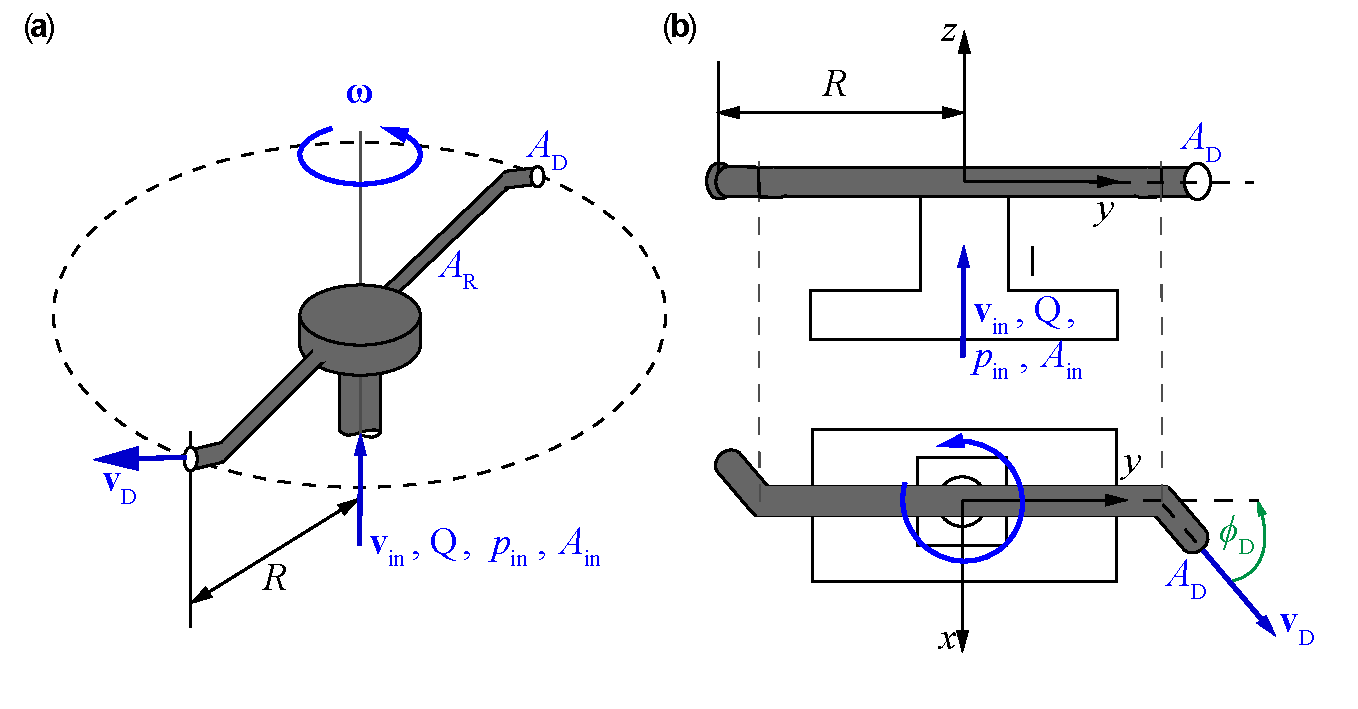
\includegraphics[width=\textwidth]{RegularSprinkler.pdf}
    \caption[Physik am Rasensprinkler.]{Physik am Rasensprinkler. \fa Prinzipaufbau und physikalische Gr��en. \fb Geometrie. Die D�sen haben einen Winkel $\phi_\text{D}$ relativ zur Tangente des durch die horizontalen Arme definierten Kreises. }
    \label{abb:kontmech_sprinkler01}
  \end{figure}
	
\begin{enumerate} 
\item [a)] \textbf{Drehzahl}\\
Mit \figref{kontmech_sprinkler01} k�nnen wir im Inertialsystem, den Drehimpuls-Drehmomenten-Satz aufschreiben.\\
\begin{align}
    \frac{\d}{\d t}\,\vec{L} = \frac{\d}{\d t}\,\lek \vec{L}_{\lk\text{Vol}\rk} + \vec{L}_{\lk\text{Aussto�}\rk}\rek = \vec{M}_{\text{Reibung}}\,. \label{kontmech_sprinkler01}
\end{align}
$\d/\d t\,\vec{L}_{\lk\text{Vol}\rk}$ ist die �nderung des Gesamtvolumens des flie�enden Wassers im Sprinkler und $\d/\d t\,\vec{L}_{\lk\text{Aussto�}\rk}$ die entsprechende Drehimpuls�nderung durch das aus der D�se ausgesto�ene Wasser. $\vec{M}_{\text{Reibung}}$ ist das Reibungsmoment.\\
Wir schreiben genauer:
\begin{align}
    \underbrace{\frac{\d}{\d t}\,\int\limits_{\lk\text{Vol}\rk}\varrho\,\vec{r}\times\vec{v}\,\D V}_{I_1} + \underbrace{\int\limits_{\lk{2 A_\text{D}}\rk}\varrho\,\vec{r}\times\vec{v}\,\lk \vec{v}_\text{D}-\vec{v}_\text{S}\rk\,\D \vec{Q}}_{I_2} =-\eta\,\vec{\omega} = -\eta\,\omega\,\veceZ\,.\label{kontmech_sprinkler02}
\end{align}
$\eta$ ist ein Koeffizient der Reibung. \\
Im station�ren Fall ist $I_1=0$. Das zweite Integral $I_2$ wird ermittelt, indem �ber die Querschnittsfl�che $A_\text{D}$ der D�sen�ffnung integriert wird. $\vec{v}_\text{D}$ ist die Geschwindigkeit des Wassers an der die D�sen�ffnung und $\vec{v}_\text{S} = \omega\,R\,\vec{e}_\phi$ die aus der Rotation resultierende Geschwindigkeit des Sprinklerarms am Ort der D�se, $Q$ ist der gesamte station�re Fluss durch die zwei Austrittsfl�chen $A_\text{D}$.\\
Die f�r den Drehimpuls relevante Austrittsgeschwindigkeit in Richtung $\vec{e}_\phi$ im Inertialsystem ist dann:
\begin{align}
    \vec{v}_\text{D}-\vec{v}_\text{S} = \frac{Q}{2}\,\frac{1}{A_\text{D}}\,\cos\phi_\text{D}\,\vec{e}_\phi-\omega\,R\,\vec{e}_\phi\,,\label{kontmech_sprinkler03}
\end{align}
worin $\phi_\text{D}$ der Winkel der D�senrichtung zur Tangente an den Kreis mit Radius $R$ (\figref{kontmech_sprinkler01})\,b ist. Damit erhalten wir f�r den station�ren Fall aus \eqref{kontmech_sprinkler02} einfach
\begin{align}
    I_2 = 2\varrho\,\frac{Q}{2}\,\lek \lk R\,\vec{e}_\text{r} \times \frac{Q}{2A_\text{D}}\,\cos\phi_\text{D}-\omega\,R\rk\,\vec{e}_\phi \rek = \eta\,\omega\,\veceZ\,. \label{kontmech_sprinkler04}
\end{align}
Hieraus erhalten wir schlie�lich
\begin{align}
    \omega= \frac{Q\,\cos\phi_\text{D}}{2A_\text{D}\,\lek R+\eta/\lk\varrho\,Q\,R\rk\rek}\,. \label{kontmech_sprinkler05}
\end{align}

Wir machen noch zum Vergleich die analogen Betrachtungen im mitbewegten Koordinatensystem, wobei wir wieder vom station�ren Fall ausgehen. Aus Gleichung \eqref{kontmech_sprinkler02} wird:
\begin{align}
    I_2 = \int\limits_{\lk{2A_\text{D}}\rk}\varrho\,\vec{r}\times\vec{v}_\text{D}\,\D Q = \vec{M}_\text{Reibung}+ \vec{M}_\text{Tr�gheit}\,.\label{kontmech_sprinkler06}
\end{align}
Hier haben wir auf der rechten Seite ein zus�tzliches Drehmoment ber�cksichtigt, was aus den Tr�gheitskr�ften (speziell der Coriolis-Kraft) im mitbewegten System resultiert. Wir werten \eqref{kontmech_sprinkler06} aus und erhalten:
\begin{align}
\begin{split}
    2\varrho\,\frac{Q}{2}\,\lek R\,\vec{e}_r \times \frac{Q}{2A_\text{D}}\,\cos\phi_\text{D}\,\vec{e}_\phi \rek &= -\eta\,\omega\,\veceZ + \int\limits_{\lk{\text{Vol}}\rk} \varrho\,\vec{r}\times\vec{f}_\text{Cor}\,\,\D V \\
    &= \eta\,\omega\,\vec{e}_z + \int\limits_{\lk{\text{Vol}}\rk} \varrho\,r\,2\omega\,v_\text{r} \,\,\D V\,\vec{e}_z
\end{split}\label{kontmech_sprinkler07}
\end{align}
mit $v_r = \vec{v}\,\vec{e}_r = Q/2A_r$ als die Str�mungsgeschwindigkeit des Wassers in den Sprinklerarmen (deren Querschnittsfl�che ist $A_r$) und der Corioliskraftdichte
\begin{align}
    \vec{f}_\text{Cor} = -2\omega\,v_r\,\vec{e}_{\phi} \,.\label{kontmech_sprinkler08}
\end{align}
Es wird \eqref{kontmech_sprinkler07} �ber das Volumenelement $\D V =A_r \,\D r$ integriert, woraus folgt:
\begin{align}
    -\varrho\,\frac{Q^2}{2A_\text{D}}\,R\,\cos\phi_\text{D} = -\eta\,\omega - 2\,\varrho\,\omega\,Q\,\int\limits_0^\text{R} r\,\D r\,. \label{kontmech_sprinkler09}
\end{align}
Hier haben wir bei der Integration �ber die Corioliskraftdichte einen Faktor 2 ber�cksichtigt, da die Corisoliskraft in den beiden Armen des Sprinklers in gleicher Weise wirkt und wir nur �ber eine Arml�nge von $0$ bis $R$ integrieren. 
Nach Umformung erhalten wir wieder:
\begin{align}
    \omega = \frac{Q\,\cos\,\phi_\text{D}}{2A_\text{D}\,\lek R+\eta / \lk \varrho\,Q\,R\rk\rek}\,, \label{kontmech_sprinkler10}
\end{align}
was nat�rlich mit \eqref{kontmech_sprinkler05} �bereinstimmt.\\
Wenn man eine station�re Umdrehungszahl von \ca $\SI{30}{\per\minute} = \SI{0.5}{\per\second}$ annimmt, erh�lt man f�r typische Werte $R=\SI{30}{\cm}$, $A_\text{D}  = \pi/4\,d_\text{D}{}^2 = \pi/4\,\SI{4}{\square\mm}$, $Q = \SI{0.1}{\cubic\dm\per\second}$, $\phi_\text{D} = 10\degree$ und $\varrho \approx \SI{1}{\kg\per\cubic\metre}$ f�r das Reibungsmoment 
\begin{equation}
	\eta = Q\,R\,\varrho\,\lek \frac{Q\,\cos\phi_\text{D}}{2A_\text{D}\,\omega}-R \rek \approx \SI{0.1}{\newton\metre\second} \,.\\ 
	\label{kontmech_sprinkler10a}
\end{equation}
Man kann sich die Fragen stellen, wie gro� $\omega$ wird, wenn die Reibung $\eta$ gegen $0$ geht? Aus \eqref{kontmech_sprinkler10} erhalten wir
    \begin{align*}
        \omega = \frac{Q\,\cos\phi_\text{D}}{2A_\text{D}\,R} ~~~~\rightarrow ~~~~ v = \omega\,R\approx\frac{Q\,\cos\phi_\text{D}}{2A_\text{D}} = v_\text{D}\,\cos\phi_\text{D}\,.
    \end{align*}
Die Tangentialgeschwindigkeit des Sprinklers am Ort der D�se wird also gleich der Ausstr�mgeschwindigkeit, was ja auch zu erwarten war.\\

\item [b)] \textbf{Wasserdruck}\\

Welchen Wasserdruck braucht man, damit bei einem Reibungskoeffizienten von $\eta=\SI{10}{\newton\metre\second}$ eine Rotationsfrequenz von $\omega = 30\ldots60\,\SI{}{\per\minute}$ zustande kommt? \\
Wir m�ssen dazu das Bernoulli-Gesetz im mitrotierenden System anwenden, da wir nur dort einen station�ren Punkt f�r die D�se und damit Anwendung des Bernoulli-Gesetzes finden k�nnen. Wir erhalten dann mit \figref{kontmech_sprinkler01}\,b:
    \begin{align}
        p_\text{L} + \underbrace{\frac{1}{2}\,\varrho\,v_\text{D}{}^2-\frac{1}{2}\,\varrho\,\omega^2\,R^2}_{\text{Ort: D�se}} = \underbrace{p_\text{in} + \frac{1}{2}\,\varrho\,v_\text{in}{}^2}_{\text{Ort: Inlet}} \,. \label{kontmech_sprinkler11}
    \end{align}
    Der dritte Term auf der linken Seite mag etwas �berraschen. Da wir aber im bewegten System sind, ist dies nichts anderes als der Druck, der durch die Zentrifugalkraft des ausstr�menden Wassers aus dem rotierenden Sprinkler hervorgerufen wird. Dieser Wert ist auch dann vorhanden, wenn der Sprinkler rotiert und der Einlass blockiert wird.
    Wir setzen $v_\text{D} = Q/A_\text{D}$, $v_\text{in} = Q/A_\text{in}$ und $p_\text{L}\approx \SI{1013e2}{\Pa}$.
    Dann folgt:
    \begin{align}
        \Delta p = p_\text{in} - p_\text{L} = \frac{1}{2}\,\varrho\,\lek \frac{Q^2}{{A_\text{D}}^2}-\frac{Q^2}{{A_\text{in}}^2}-\omega^2\,R^2\rek\,. \label{kontmech_sprinkler12}
    \end{align}
    Damit eine Rotation zustande kommt muss offensichtlich $\Delta p > 0$ und $A_\text{D}<A_\text{in}$ sein und der Flu� 
    \begin{align*}
        Q = \frac{\omega R A_\text{D}}{\sqrt{1-A_\text{D}{}^2/A_\text{in}{}^2}}\,.
    \end{align*}
		Mit unseren Werten von oben und $A_\text{in}  = \pi/4\,\SI{1.25}{\square\cm}$, erhalten wir $\Delta p/p_\text{L} \approx 1.3$, siehe dazu auch \figref{kontmech_sprinkler02}.\\
		
		
	\begin{figure}
    \centering
    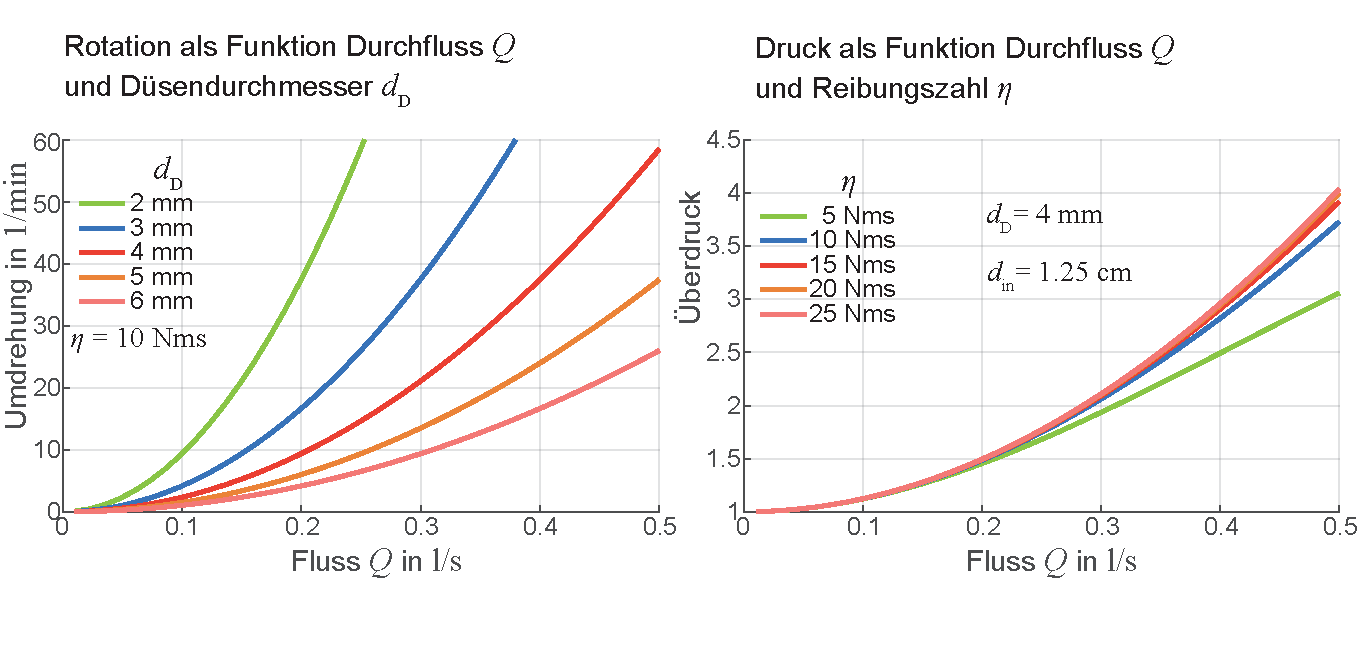
\includegraphics[width=\textwidth]{RegularSprinkler02.pdf}
    \caption[Physik am Rasensprinkler.]{Physik am Rasensprinkler. Berechnung verschiedener Parameter.}
    \label{abb:kontmech_sprinkler02}
  \end{figure}


\item [c)] \textbf{Blockierter Gartenschlauch}\\

Warum schie�t das Wasser aus einem Sprinkler \bzw einem Wasserschlauch h�her \bzw weiter, wenn man die  �ffnung teilweise blockiert? Diese scheinbar einfache Frage ist gar nicht so einfach zu beantworten. Eine alleinige Betrachtung mit der Bernoulli-Gleichung reicht nicht aus, da wir bei diesem Problem die Viskosit�t der Fl�ssigkeit mit ber�cksichtigen m�ssen. Wir empfehlen den interessierten Leser die analytischen und numerischen Betrachtungen in \cite{Alam2021} und geben hier nur eine anschauliche Erkl�rung an:\\        
Wird ein Gartenschlauch an der Ausgangs�ffnung teilweise blockiert, so kommt es zu einer Reduktion des Volumenflusses $Q$ innerhalb des Schlauches, damit auch zu einer geringeren viskosen Reibung im Schlauch und damit einen geringeren Druckabfall. Vergleiche dazu \eqref{eq:kontmech_StroemungsGeschwKreisrohr} (Gesetz von Hagen\footnote{Gotthilf Heinrich Ludwig Hagen (1797--1884) war ein deutscher Wasserbauingenieur und Hochschullehrer. Er gab das erste in deutscher Sprache erschienene Handbuch der Wasserbaukunst heraus.}\indexp{Hagen, Gotthilf Heinrich Ludwig}-Poiseuille\footnote{Jean L�onard Marie Poiseuille (1797-�1869) war ein franz�sischer Physiologe und Physiker. Er arbeitete vorwiegend auf dem Gebiet der Physiologie des Blutkreislaufs und versuchte physikalische  Erkenntnisse auf die Physiologie zu �bertragen.}\indexp{Poiseuille, Jean L�onard Marie}\index{Gesetz von Hagen-Poiseuille} genannt). Es steht also mehr Druck zur Verf�gung, der die Fl�ssigkeitsteilchen am Ende des Schlauches auf eine h�here  Geschwindigkeit beschleunigt.
\end{enumerate}

\end{sol} 
\textcolor{blue} {$\rightarrow$ zur} \probref{kontmech_rotating_sprinkler}.\\
\noindent\rule[1ex]{\textwidth}{0.5pt}  \newpage  \clearpage


%-----------------------------------------------------------------------------------------------------------


\begin{sol}{prob:kontmech_reverse_sprinkler}\label{lsg:kontmech_reverse_sprinkler} %�bung9
\textbf{Feynmans inverser Rasensprinkler}\\ \\

Eine gute Darstellung des Diskussionsstands zu allen Effekten, die uns in
dieser Aufgabe interessieren, findet sich bei Jenkins \cite{Jenkins2004}.
Tats�chlich zeigt eine neuere, sehr detaillierte Betrachtung, dass f�r ein
vollst�ndiges Bild die Geometrie in Verbindung mit Reibungseffekten sehr
genau analysiert werden muss, um mit experimentellen Beobachtungen in
Einklang zu kommen \cite{Wang2024}.

Im wesentlichen l�sst sich die Tatsache, dass der inverse Sprinkler (abgesehen
vom Anlaufen und Anhalten des Wasserflusses und ohne die asymmetrischen Effekt
aus \cite{Wang2024}) nicht zu einer Drehung angeregt wird, mit seiner
besonderen Konstruktion begr�nden. Eine vereinfachte L-f�rmige Darstellung
eines Arms des Sprinklers als wesentliches Bauteil, an dem erkl�rt werden kann,
dass das Drehmoment verschwindet, ist nach der Idee von Jenkins
\cite{Jenkins2004} in \figref{kontmech_inverserSprinklerKonstr} zu sehen.
Tats�chlich verschwindet allein schon an einem Arm das resultierende
Drehmoment. Es handelt sich nicht um einen Effekt des Ausgleichs mehrerer Arme.

\begin{figure}
  \centering
  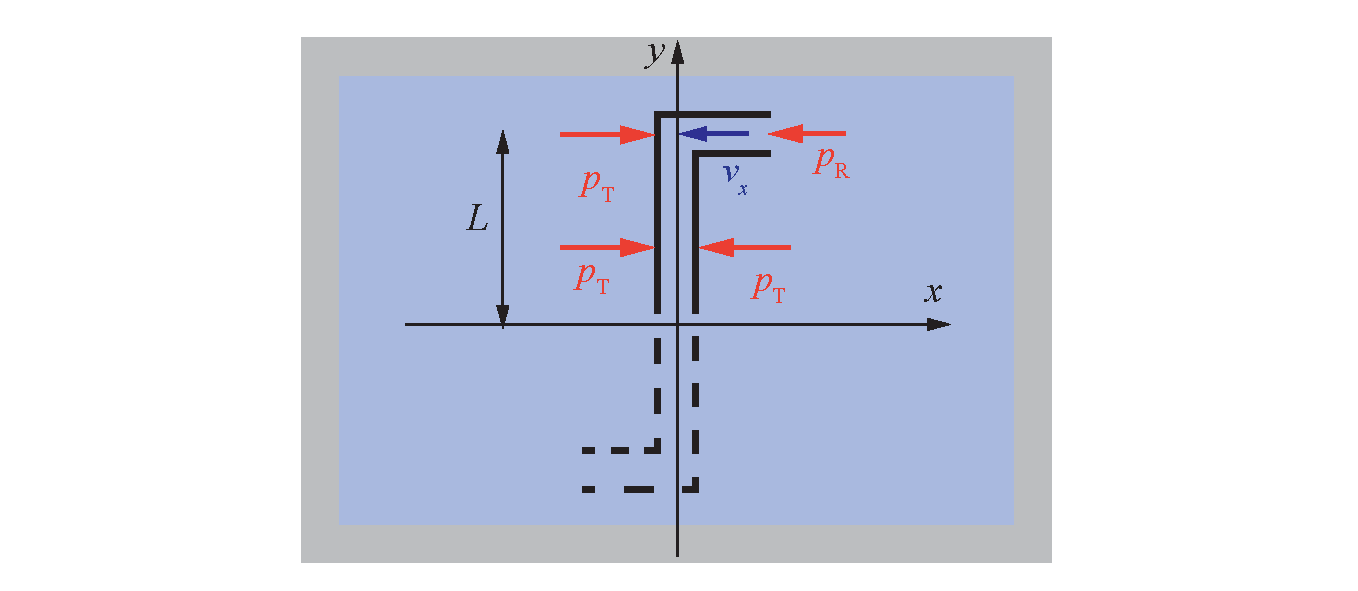
\includegraphics[width=\textwidth]{InverserSprinklerDruck.pdf}
  \caption[Aufbau des inversen Sprinklers mit Druckbilanz.]%
  {Aufbau des inversen Sprinklers mit Druckbilanz und Geschwindigkeit,
    die zu einer Impuls�nderung f�hrt.}
  \label{abb:kontmech_inverserSprinklerKonstr}
\end{figure}

Betrachten wir zun�chst die Druckbilanz, wie in der Aufgabenstellung
vorgeschlagen wird. Das Wasser des inversen Sprinklers wird in der
Beschreibung Feynmans durch eine Saugpumpe angetrieben. Somit handelt es sich
um eine Wasserbewegung, die von einem Druckuntrschied am Laufen gehalten
wird. Der Druck $p_\mathrm{R}$ im Saugrohrarm muss also geringer sein als
der Druck $P_\mathrm{T}$ im Tank, der von allen Seiten auf den Sprinklerarm
wirkt. Damit ergibt sich mit einem Rohrquerschnitt der Fl�che $A$ eine
resultirende Kraft
\begin{equation*}
  F_\mathrm{D} = (p_\mathrm{T}-p_\mathrm{R})\,A
\end{equation*}
durch den Druckunterschied auf die Wand. Mit der Arml�nge $l$ (die wir bis
zur Mitte auf der angreifenden Fl�che $A$ messen), erhalten wir daraus
ein Drehmoment von
\begin{equation*}
  M_\mathrm{D} = (p_\mathrm{T}-p_\mathrm{R})\, A\, L \; .
\end{equation*}

W�rde nur das Drehmoment durch den Druckunterschied bestehen, m�sste der
Sprinkler sich beschleunigt drehen, bis eine Reibungskraft im Gleichgewicht
zur Beschleunigung steht. Wir m�ssen jedoch auch ber�cksichtigen, dass
das Wasser an der Fl�che $A$ seine Flussrichtung �ndert. Das einstr�mende
Wasser hat einen Impuls in negative $x$-Richtung. Dieser Impuls muss
vollst�ndig abgebremst werden, was einen weitere Kraft auf den Arm
bewirkt.\footnote{Nat�rlich nimmt das Wasser auch einen Impuls in negativer
  $y$-Richtung auf, jedoch muss dieser uns nicht interessieren, da die daf�r
  notwendige Kraft vom Fu� des Sprinklers aufgebracht wird und zus�tzlich
  parallel zum Arm verl�uft und somit kein Drehmoment aus�ben kann.}
Diese Kraft k�nnen wir direkt aus der Impuls�nderung des Wassers ableiten.
Dabei ist die Kraft auf das Rohr negativ zu der, die das Rohr auf das
Wasser aus�ben muss, um dieses abzubremsen, also
\begin{equation*}
  F_\mathrm{I} = -\frac{\D m_\mathrm{W}\,v_x}{\D t} = -\frac{\D m_\mathrm{W}}{\D t}\, v_x \; .
\end{equation*}
Das Str�mungsverhalten an der Rohr�ffnung ist sicher komplex. Wir k�nnen
uns jedoch auf die Massenerhaltung verlassen. Damit die Str�mung im Rohr
station�r sein kann (und genau diesen Fall betrachten wir bisher), muss im
Zeitintervall $\D t$ gerade so viel im Tank stehendes Wasser auf die
Flie�geschwindigkeit $v_x$ im Rohr beschleunigt werden, wie im Rohr am Knick
umgelenkt wird und an $x$-Impuls verliert. Diese Beschleunigung des Wasservolumens 
geschieht aber gerade durch den Druckgradienten, sodass auch gilt
\begin{align*}
  \frac{\D m_\mathrm{W}\, v_x}{\D t} = \frac{\D m_\mathrm{W}}{\D t}\, v_x
  = F_\mathrm{D} = (p_\mathrm{T}-p_\mathrm{R})\, A \; .
\end{align*}
In Summe erh�lt man, dass $F_\mathrm{I} = - F_\mathrm{D}$, die Kraft durch den
Impuls�bertrag wirkt also genau der Kraft durch den Druckunterschied entgegen.
Gleiches gilt f�r die Drehmomente, $M_\mathrm{I} = - M_\mathrm{D}$. Der
Drehimpuls bez�glich des Fu�es des Sprinklers ist also konstant. Ist er zu
Beginn Null, bleibt er es und es kommt keine Rotation zustande.

Das war bisher nur der station�re Fall. Nun wollen wir den Anlaufprozess
betrachten. Bei diesem besteht durch die eingeschaltete Pumpe bereits
der Druckgradient. Bis das Wasser jedoch so beschleunigt wurde, dass die
Str�mung das erste Mal auf die Wand des Sprinklers am Knick trifft, fehlt
jedoch der Impuls�bertrag, der die Kraft aufgrund des Druckunterschieds
ausgleichen k�nnte. Es kommt zu einer Beschleunigung in Richtung des
offenen Endes des Rohres. Der Sprinkler bewegt sich im Uhrzeigersinn.

Genau das Gegenteil passiert beim Abschalten. Hier bricht der Druckunterschied
schlagartig ab. Das Wasser ben�tigt jedoch einige Zeit, um zum Stillstand
zu kommen. Kurzzeitig wird die Kraft aus dem Impuls�bertrag nicht ausgeglichen
und es kommt zu einer Beschleunigung vom offenen Ende weg. Insgesamt erh�lt
man damit folgendes ideales Bewegungsbild f�r einen Fall ohne Reibung: Durch
den Anlaufprozess wird eine Kreisbewegung im Uhrzeigersinn in Gang gesetzt.
Nach dem Anlaufprozess gibt es keine Beschleunigung mehr und die Kreisbewegung
setzt sich mit konstanter Winkelgeschwindigkeit fort. Mit dem Abschalten der
Pumpe kommt diese Kreisbewegung wieder zum Stehen.

Geht man genauer auf die Form und die Anordnung der D�sen ein \cite{Wang2024}, stellt sich heraus, dass
sich in der Geometrie nach \figref{kontmech_inverserSprinklerKonstr} unter Ber�cksichtigung von Reibungseffekten beim Ansaugen des
Wassers ein asymmetrischen Geschwindigkeits- \bzw Druckprofil herausbilden kann,
 \dh es gilt nicht �berall $p_\mathrm{T}=\con$. Genaueres
�berlegen f�hrt dazu, dass ein solches sogar ziemlich wahrscheinlich ist, denn das
Wasser muss ja die Biegung im Arm umstr�men. Eine solche Asymmetrie f�hrt aber
nun dazu, dass es doch ein resultierendes effektives (kleines) Drehmoment gibt, das (auch im
station�ren Fluss) eine Drehbewegung verursachen kann.\\
Dem interessierten Leser empfehlen wir die Darstellung der aktuellen "`Forschungsergebnisse"' zu dem Thema in \cite{Wang2024}.

\end{sol} 
\textcolor{blue} {$\rightarrow$ zur} \probref{kontmech_reverse_sprinkler}.\\
\noindent\rule[1ex]{\textwidth}{0.5pt}  \newpage  \clearpage

%-----------------------------------------------------------------------------------------------------------

\begin{sol}{prob:kontmech_StroemungRechteckrohr}\label{lsg:kontmech_StroemungRechteckrohr} %�bung10
\textbf{Str�mung durch Rohre}\\ \\

\begin{enumerate}

\item F�r die Str�mung durch ein Rohr, muss die Differentialgleichung
  \eqref{eq:kontmech_NaStstat}, 
  \begin{equation*}
    \eta \, \Delta \vec{v} - \nablav p = \vec{0} \; ,
  \end{equation*}
  f�r eine Fl�che senkrecht zur Str�mung gel�st werden. Wenn wir die
  Fl�che parallel zur $x$-$y$-Ebene ansehen und f�r eine station�re
  Str�mung annehmen, dass $\vec{v} = v_z(x,y) \veceZ$, also die $v_z$-Komponente
  selbst nicht von $z$ abh�ngt (vergleiche Beispiel
  \ref{bsp:kontmech_laminareStroemungen} in Kapitel
  \ref{kap:kontmech_laminareStroemungenFluessigkeiten}), so reduziert
  sich die Differentialgleichung auf
  \begin{equation*}
    \eta \, \left ( \frac{\partial^2}{\partial x^2} + \frac{\partial^2}
      {\partial y^2} \right ) v_z = \frac{\partial p}{\partial z}
  \end{equation*}
  mit einem konstanten Druckgradienten in $z$-Richtung.

  Diese partielle Differentialgleichung wird mit Hilfe der Partial
  Differential Equation Toolbox von \matlab{} gel�st und zwar mit der 
  \textcolor{mygreen}{\texttt{solvepde}}-Routine.
  Die Kreisgeometrie
  wird mit der vordefinierten Kreisfl�che des Radius 1 (entspricht in
  unserem Fall $\SI{1}{\metre}$) beschrieben. Dar�ber hinaus werden die
  Zahlenwerte $a = \SI{20}{\centi\metre}$, $b = \SI{30}{\centi\metre}$,
  $\eta = 1$ (Wasser) sowie ein angenommener geringer Druckgradient von
  $\partial p/\partial z = \SI{20}{\pascal\per\metre}$ verwendet. Das
  Beispielprogramm ist in der \matlab{}-Datei \mlkontmechref{Kreisrohr.m}
  gegeben.

  Man erh�lt die in \figref{kontmech_KreisRohrGeschwindigkeit} dargestellte
  L�sung. Der Paraboloid, den wir bereits aus Beispiel
  \ref{bsp:kontmech_laminareStroemungen} kennen, ist deutlich zu erkennen.
  Daneben ist die Differenz der numerischen und der analytischen L�sung
  aus Gleichung \eqref{eq:kontmech_StroemungsGeschwKreisrohr} gezeigt. Sie f�llt
  so klein aus, dass sie allein durch numerische Fehler zu erkl�ren ist.  
  
  \begin{figure}
    \centering
    \includegraphics[width=\textwidth]{KreisRohrGeschwindigkeit.pdf}
    \caption[Geschwindigkeitsprofil einer Str�mung in einem kreisrunden Rohr.]
    {\fa Geschwindigkeitsprofil der Str�mung durch ein kreisrundes Rohr bei einem
      konstanten Druckgradienten senkrecht zum Rohrquerschnitt. \fb Differenz zwischen der numerischen Berechnung und der
      analytischen L�sung aus \eqref{eq:kontmech_StroemungsGeschwKreisrohr}. Siehe \mscr~ \mlkontmechref{Kreisrohr.m}}
    \label{abb:kontmech_KreisRohrGeschwindigkeit}
  \end{figure}

  
\item Nun muss dieselbe Differentialgleichung auf einem rechteckigen Gebiet
  gel�st werden, das wir durch $-a/2 < x < a/2$ und $-b/2 < y < b/2$
  beschreiben. Auf dem Rand m�ssen die Dirichlet-Randbedingungen
  $v_z(-a/2,y) = v_z(a/2,y) = v_z(x,-b/2) = v_z(x,b/2) = 0$ erf�llt sein.

  Mit diesen Angaben und denselben Zahlenwerten wie im vorherigen
  Aufgabenteil erh�lt man das Beispiel, das im \matlab{}-Programm
  \mlkontmechref{Rechteckrohr.m} gegeben ist. Das Ergebnis ist in
  \figref{kontmech_RechteckRohrGeschwindigkeit} dargestellt.

  \begin{figure}
    \centering
    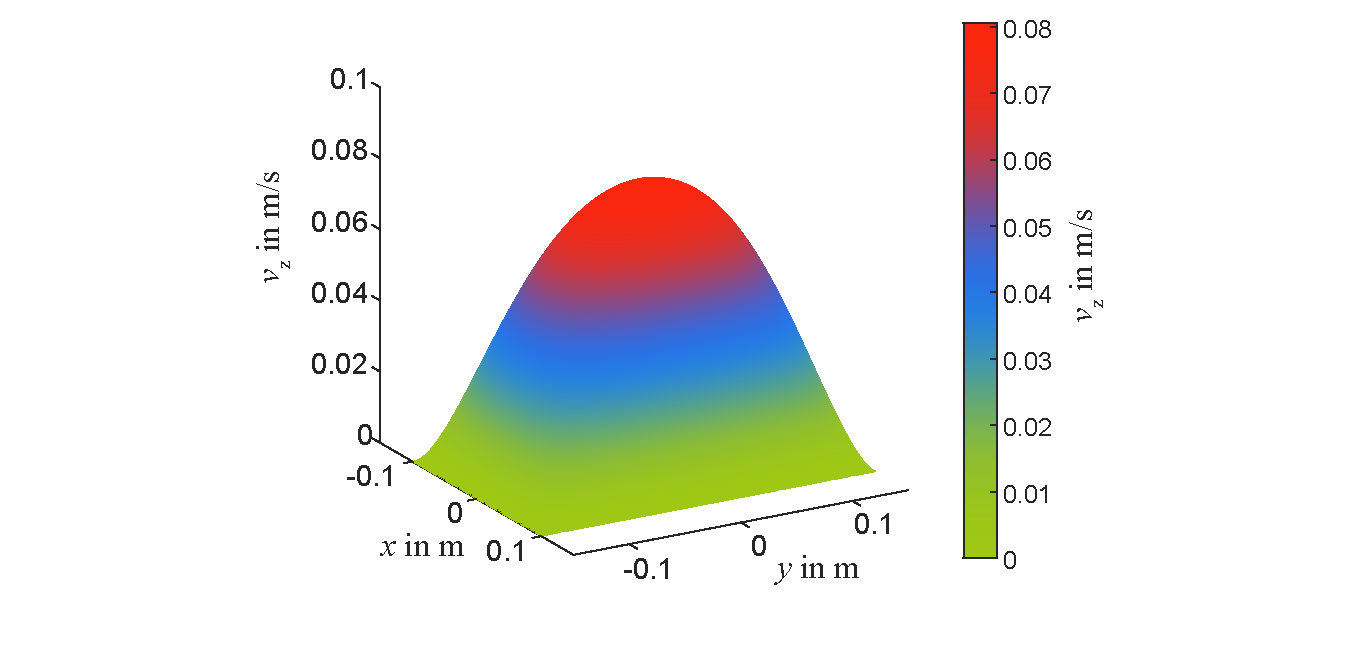
\includegraphics[width=0.8\textwidth]{RechteckRohrGeschwindigkeit.pdf}
    \caption[Geschwindigkeitsprofil einer Str�mung in einem rechteckigen Rohr.]
    {Geschwindigkeitsprofil der Str�mung durch ein rechteckiges Rohr bei einem
      konstanten Druckgradienten senkrecht zum Rohrquerschnitt.}
    \label{abb:kontmech_RechteckRohrGeschwindigkeit}
  \end{figure}
  �hnlich der L�sung im kreisrunden Rohr liegt in der Mitte
  des Rohres die h�chste Geschwindigkeit vor. Zu den R�ndern hin f�llt
  sie rasch ab. Anders als im runden Rohr ist der Abfall jedoch nicht rein
  quadratisch. Insbesondere findet man, dass er auf den Diagonalen, entlang
  derer der Weg von der Mitte zur Wand am gr��ten ist, langsamer ist als in
  der Mitte der Kanten. In den Ecken flacht das Profil erkennbar ab.
\end{enumerate}


\end{sol} 
\textcolor{blue} {$\rightarrow$ zur} \probref{kontmech_StroemungRechteckrohr}.\\
\noindent\rule[1ex]{\textwidth}{0.5pt}  \newpage  \clearpage

%-----------------------------------------------------------------------------------------------------------

\begin{sol}{prob:kontmech_StroemungTorricelli}\label{lsg:kontmech_StroemungTorricelli} %�bung11
\textbf{Str�mung aus einer Tonne - Gesetz von Torricelli}\index{Torricelli-Gesetz}\\ \\

Zur Herleitung geht man von der Bernoulli-Gleichung \index{Bernoulli-Gleichung} aus:
Man macht die Annahme, dass der Beh�lter gro� ist, so dass sich der Wasserspiegel kaum �ndert. 
Die Gr��en mit dem Index 1 gelten an der Wasseroberfl�che, die Gr��en mit dem Index 2 am Ausfluss. An der Oberfl�che ist die Geschwindigkeit $v_1$ (fast) null. Legt man die $x$-Achse in den Ausfluss, ist $h_2=0$ und $h_1$ entspricht dem H�henunterschied $H$. Der Umgebungsdruck $p_0$ sei oben und unten ann�hernd gleich gro�. Somit vereinfacht sich die Bernoulli-Gleichung zu:
\begin{align*}
\frac{v_1{}^2}{2} +\frac{p_1}{\varrho} + g\,h_1 &= \frac{v_2{}^2}{2} +\frac{p_2}{\varrho} + g\,h_2\\
\rightarrow~~~\frac{p_0}{\varrho} + g\,H &= \frac{v_2{}^2}{2} +\frac{p_0}{\varrho} \\
\rightarrow~~~\frac{p_0}{\varrho} + g\,H &= \frac{v_2{}^2}{2} +\frac{p_0}{\varrho} ~~\rightarrow v_\text{A} = v_2 =\sqrt{2g\,H}\,.\\
\end{align*}
In der Formel f�r die Austrittsgeschwindigkeit taucht der Querschnitt der Austritts�ffnung nicht auf. Damit ist auch der Auftreffpunkt des Wasserstrahls nicht von diesem Querschnitt abh�ngig. In der Praxis treten nat�rlich durch die Form der Austritts�ffnung (z.B. verrundet oder scharfkantig) und durch die Einschn�rung des Wasserstrahls teilweise starke Abweichungen der Austrittsgeschwindigkeit vom theoretischen Wert auf. Trotzdem zeigen auch viele eine verbl�ffende �bereinstimmung.

Diese Formel wurde von dem italienischen Mathematiker und Physiker Evangelista Torricelli\indexp{Torricelli, Evangelista} gefunden und nach ihm benannt.\index{Torricelli-Gleichung}

Um das Str�mungsfeld  zu berechnen, schreiben wir die Navier-Stokes-Gleichung
\eqref{eq:kontmech_NavierStokes} f�r den Fall auf, dass das Geschwindigkeitsfeld
station�r ist:
\begin{equation}
  \varrho \lk \vec{v} \cdot \nablav \rk \vec{v} = \vec{f}_\text{V}
  + \eta \, \Delta \vec{v} - \nablav p \;.
  \label{eq:kontmech_torricelli_NavierStokes}
\end{equation}
Weiterhin ber�cksichtigen wir die Konituit�tsgleichung
\eqref{eq:kontmech_KontinuitaetsglDiff}, wobei im Tank keinerlei Quellen
oder Senken existieren sollen und die Fl�ssigkeit inkompressibel sei ($\varrho =
\text{const}$):
\begin{equation}
  \frac{\partial}{\partial t}\varrho + \divv \lk \varrho\, \vec{v} \rk
  \varrho \divv \vec{v} = 0 \qquad \Rightarrow\text{d.h.} \qquad \divv \vec{v} = 0
  \; .
  \label{eq:kontmech_torricelli_kont}
\end{equation}


Die numerische L�sung des hier vorlegenden rein zweidimensionalen Problems
l�sst sich einfacher finden, wenn man das Geschwindigkeitsfeld $\vec{v}$
durch die Stromfunktion $\vec{u}$ und den Wirbelvektor $\Omega$ nach \eqref{eq:kontmech_Wirbelvektor}
ausdr�ckt. F�r die Stomfunktion gilt: 
\begin{equation}
  \vec{v} = \rotv \vec{u}
  \label{eq:kontmech_Stromfunktion}
\end{equation}
Das Einf�hren der Stromfunktion \eqref{eq:kontmech_Stromfunktion}
ist insbesondere m�glich, da sich $\vec{v}$ aufgrund der Kontinuit�tsgleichung
\eqref{eq:kontmech_torricelli_kont} als Rotation eines Vektorfeldes darstellen
lassen muss. Durch diese Darstellung ist die Kontinuit�tsgleichung automatisch
erf�llt und muss nun nicht weiter betrachtet werden.

Wir legen das Koordinatensystem so, dass die $x$-Achse in die horizontale
Richtung zeigt und die vertikale Richtung durch die $y$-Achse beschrieben
wird. Der Ursprung liegt in der linken unteren Ecke des Tanks. In diesem
Fall k�nnen wir im vorliegenden zweidimensionalen Problem
\begin{equation}
  \vec{u} = u(x,y)\veceZ
  \label{eq:komtech_torricelli_ansatzu}
\end{equation}
ansetzen und erhalten
\begin{align*}
  v_x &= \frac{\partial u}{\partial y} \;,~~~~
  v_y = -\frac{\partial u}{\partial x} \; .
\end{align*}
Weiterhin erhalten wir
\begin{equation*}
  \vec{\Omega} = \frac{1}{2} \rotv \vec{v} = \frac{1}{2} \rotv \rotv \vec{u}
  = \frac{1}{2} \lk \gradv \divv \vec{u} - \Delta \vec{u} \rk \; ,
\end{equation*}
was sich mit \eqref{eq:komtech_torricelli_ansatzu} auf
\begin{equation*}
  \vec{\Omega} = - \frac{1}{2} \Delta u(x,y)\veceZ
\end{equation*}
reduziert. Das hei�t, wir haben
\begin{equation}
  \vec{\Omega} = \Omega(x,y) \veceZ ~~~\text{und}~~~
  \Omega(x,y)  = -\frac{1}{2} \Delta u = -\frac{1}{2} \lk \frac{\partial^2}
  {\partial x^2} + \frac{\partial^2}{\partial y^2} \rk u \; .
  \label{eq:kontmech_torricelli_pdgl1}
\end{equation}

Um auch die Navier-Stokes-Gleichung durch $u$ und $\Omega$ auszudr�cken,
nehmen wir die Rotation von \eqref{eq:kontmech_torricelli_NavierStokes}.
Aus der vorherigen Berechung der Austrittsgeschwindigkeit wissen wir bereits,
dass die Volumenkraft (Gravitation) eine reine Gradientenkraft ist. Auch
der Druck hat nur einen Gradienten und keine Rotationskomponente. Entsprechend
fallen diese Terme weg. Das st�rt uns aber nicht. Die Randbedingungen,
wie sie sich durch den Fluss der Fl�ssigkeit im Gravitationsfeld ergeben,
sind durch die Berechnung der Geschwindigkeit der ausstr�menden Fl�ssigkeit
hinreichend gegeben. Wir haben nur noch das Ziel, das Geschwindigkeitsfeld
innerhalb des Tanks zu bestimmen. In den gew�hlten zweidimensionalen
Koordinaten reduziert sich die Navier-Stokes-Gleichung auf
\begin{equation}
  \varrho \lk \frac{\partial u}{\partial y}\frac{\partial \Omega}{\partial x}
  - \frac{\partial u}{\partial x}\frac{\partial \Omega}{\partial y} \rk
  = \eta \lk \frac{\partial^2 \Omega}{\partial x^2} + \frac{\partial^2 \Omega}
  {\partial y^2} \rk \; .
  \label{eq:kontmech_torricelli_pdgl2}
\end{equation}

Die Gleichungen \eqref{eq:kontmech_torricelli_pdgl1} und
\eqref{eq:kontmech_torricelli_pdgl2} bilden zusammen ein gekoppeltes,
partielles lineares Differentialgleichungssystem, das gel�st werden muss. Wichtig sind
dabei zus�tzlich die Randbedingungen, die erf�llt werden m�ssen, um das
korrekte Str�mungsbild zu erhalten.

Die numerische L�sung eines solchen Systems kann nicht einfach durch die in
\probref{kontmech_StroemungRechteckrohr} verwendete \matlab~Routine 
\textcolor{mygreen}{\texttt{solvepde}} erfolgen.
Man wendet f�r solche partiellen nichtlinearen Differentialgleichungssysteme
das sogenannte  SOR-Verfahren (�berrelaxationsverfahren)\index{SOR-Verfahren}\index{�berrelaxationsverfahren} an \cite{Meister2014}.  
Um zu sehen, wie dieses funktioniert, wollen wir dieses ausf�hrlich
anhand von Gleichung \eqref{eq:kontmech_torricelli_pdgl1} diskutieren.
Diese diskretisieren wir zun�chst,
\begin{equation*}
  \Omega(x_i,y_j) = -\frac{1}{2\Delta h^2} \left \{ u(x_{i+1},y_j)
    + u(x_{i-1},y_j) - 2 u(x_i,y_j) + u(x_i,y_{j+1}) + u(x_i,y_{j-1})
    - 2 u(x_i,y_j) \right \} \; ,
\end{equation*}
wobei wir davon ausgegangen sind, dass die Schrittweite in $x$- und
$y$-Richtung identisch ist und $\Delta h$ betr�gt.
Das l�sst sich umformen zu
\begin{align*}
  u(x_{i+1},y_j) + u(x_{i-1},y_j) + u(x_i,y_{j+1}) + u(x_i,y_{j-1})
  - 4 u(x_i,y_j) + 2\Delta h^2 \, \Omega(x_i,y_j)
  &= 0 \\
  \text{bzw.}~~~
  \frac{1}{4} \left \{ u(x_{i+1},y_j) + u(x_{i-1},y_j) + u(x_i,y_{j+1})
  + u(x_i,y_{j-1}) + 2\Delta h^2 \, \Omega(x_i,y_j) \right \} - u(x_i,y_j)
  &= 0 \; .
\end{align*}
F�r eine L�sung des Differentialgleichungssystems wird diese Gleichung
exakt erf�llt sein. Im SOR-Verfahren startet man mit Werten f�r die
$u(x_i,y_j)$ und $\Omega(x_i,y_j)$, die die Differentialgleichung
nicht l�sen werden. Es ergibt sich also eine nichtverschwindende Differenz
\begin{equation*}
  r^{(u)}_{ij} = \frac{1}{4} \left \{ u(x_{i+1},y_j) + u(x_{i-1},y_j)
    + u(x_i,y_{j+1}) + u(x_i,y_{j-1}) + 2\Delta h^2 \, \Omega(x_i,y_j)
  \right \} - u(x_i,y_j)
  \; ,
\end{equation*}
die gewichtet durch einen Konvergenzparameter (�berrelaxationsparameter)
\index{Konvergenzparameter}\index{�berrelaxationsparameter} $0\le s \le 2$
in einer Iteration auf den Wert von $u(x_i,y_j)$ aufaddiert wird,
\begin{equation*}
  u(x_i,y_j)^{(n+1)} = u(x_i,y_j)^{(n)} + s \, r^{(u,n)}_{ij}  \; ,
\end{equation*}
bis eine zufriedenstellende Konvergenz erreicht ist.

Analog l�sst sich f�r die zweite Differentialgleichung
\eqref{eq:kontmech_torricelli_pdgl2} ein Differenzparameter
\begin{multline*}
  r^{(\Omega)}_{ij} = \frac{1}{4} \bigg \{ \Omega(x_{i+1},y_j)
  + \Omega(x_{i-1},y_j) + \Omega(x_i,y_{j+1}) + \Omega(x_i,y_{j-1})  \\
    -\frac{\varrho}{4\,\eta} \bigg [ 
      \lk u(x_i,y_{j+1}) - u(x_i,y_{j-1}) \rk \lk \Omega(x_{i+1},y_j)
      - \Omega(x_{i-1},y_j) \rk \\
      - \lk u(x_{i+1},y_j) - u(x_{i-1},y_j) \rk \lk \Omega(x_i,y_{j+1})
      - \Omega(x_i,y_{j-1}) \rk \bigg ] \bigg \} - \Omega(x_i,y_j)
  \; ,
\end{multline*}
f�r die Iteration
\begin{equation*}
  \Omega(x_i,y_j)^{(n+1)} = \Omega(x_i,y_j)^{(n)} + s \, r^{(\Omega,n)}_{ij}  
\end{equation*}
finden.

In der Numerik verwenden wir die kinematische Viskosit�t $\nu
= \eta/\varrho$. Weiterhin bietet es sich an, die Symmetrie des Systems
auszunutzen und nur eine H�lfte des Tanks von der linken Wand bis zur Mitte
des Lochs zu berechnen. Dann ergeben sich die Randbedingungen dadurch, dass
kein Fluss durch die W�nde erfolgt und in der Mitte (also am rechten Rand des
berechneten Bereichs) ein Fluss senkrecht nach unten stattfindet. Ein Beispiel
f�r die Umsetzung, die auf \cite{Landau2018} beruht, kann in der 
\matlab{}-Datei \mlkontmechref{Torricelli.m} gefunden werden.

\begin{figure}
  \centering
  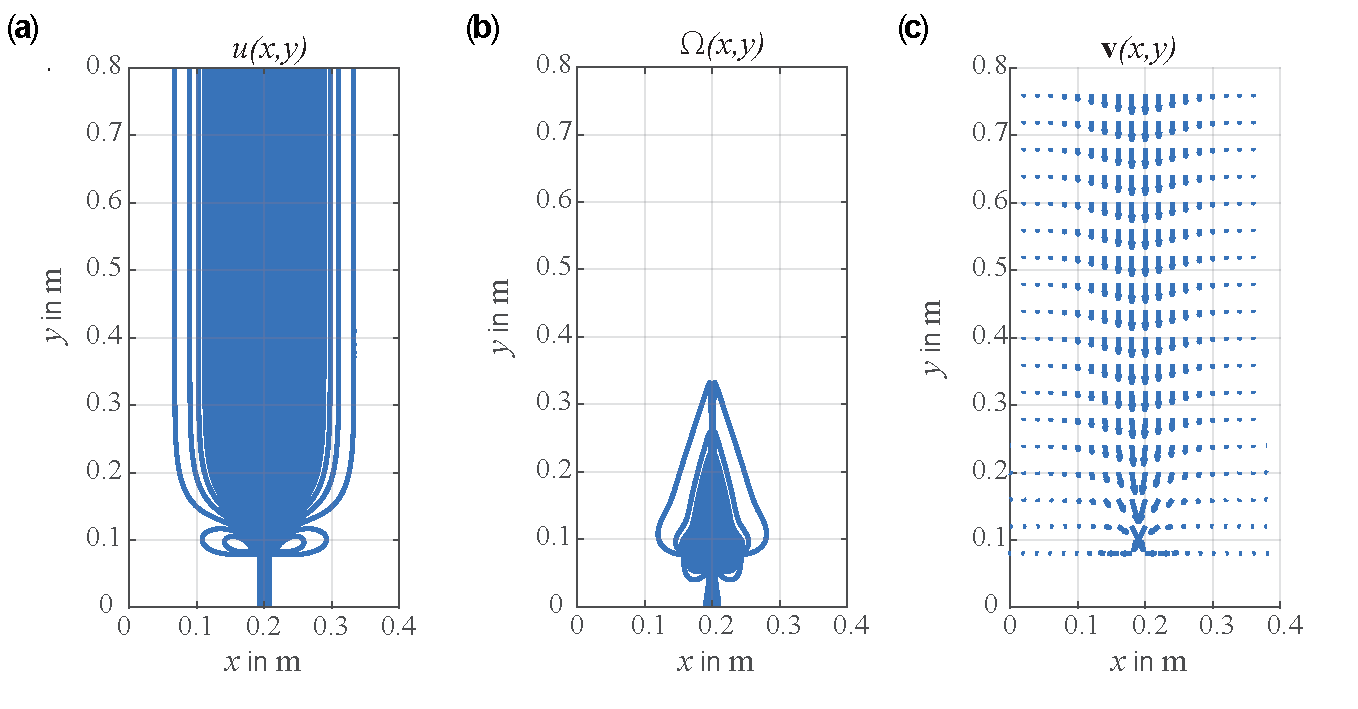
\includegraphics[width=\textwidth]{Torricelli_Fluss.pdf}
  \caption[Geschwindigkeitsprofil einer Str�mung aus einem Tank.]
  {Geschwindigkeitsprofil der Str�mung aus einem Tank bei erf�lltem Gesetz
    von Torricelli. Dargestellt sind \fa die Flusslinien (Linien mit konstantem
    $u$), \fb die Wirbellinien (Linien mit konstantem $\Omega$) sowie \fc das
    Geschwindigkeitsfeld $\vec{v}$ als Vektordiagramm.}
  \label{abb:kontmech_Torricelli_Fluss}
\end{figure}

Die Linien f�r konstantes $u$ und konstantes $\Omega$ sind in
\figref{kontmech_Torricelli_Fluss} dargestellt. Die $u$-Linien zeigen den
Fluss des Wassers an. Man erkennt das Str�men nach unten, aber auch das
Ausbilden von Wirbeln links und rechts des Ausflusses nahe am Boden. Diese
kommen dadurch zustande, dass aufgrund der Viskosit�t die zum Ausfluss
benachbarten Fl�ssigkeitsschichten mitgenommen werden. Das Nachstr�men des
Wassers f�hrt zu einer Kreisbewegung. Dem interessierten Leser wird geraten,
die kinematische Viskosit�t zu variieren, um zu beobachten, wie das zu
st�rkeren und schw�cheren Auspr�gungen der Wirbel f�hrt.

Die $\Omega$-Linien, oder Wirbellinien, zeigen an, wo der Wirbelvektor
konstant ist. Wo die Linien dicht liegen, �ndert sich der Wirbelvektor stark.
Dies ist nahe des Ausflusses der Fall und best�tigt die Beobachtung aus den
Flusslinien.

In der untersten Zeile der Abbildung sehen wir  das Geschwindigkeitsfeld als
Vektordiagramm. Es veranschaulicht noch einmal, was die Fluss- und Wirbellinien
bereits verraten. Die Fl�ssigkeit str�mt von oben zum Ausfluss, w�hrend links
und rechts von diesem am Boden Str�me zum Rand entstehen, die eine Konsequenz
der Wirbelbildung sind.

Es ist interessant, wie die Geometrie in diesem station�ren Problem zur
Ausbildung von Wirbeln f�hrt. Dem Leser wird empfohlen, den Ausfluss an die
Seite des Beh�lters zu legen, um die Ver�nderung der  Wirbelbildung zu
verfolgen. Man �berlege sich die entsprechenden Randbedingungen.


\end{sol} 
\textcolor{blue} {$\rightarrow$ zur} \probref{kontmech_StroemungTorricelli}.\\
\noindent\rule[1ex]{\textwidth}{0.5pt}  \newpage  \clearpage

%-----------------------------------------------------------------------------------------------------------

\begin{sol}{prob:kontmech_StroemungTank}\label{lsg:kontmech_StroemungTank} %�bung12
\textbf{Str�mung durch einen Tank}\\ \\

In dieser �bung k�nnen wir vollst�ndig auf die Numerik aus
\probref{kontmech_StroemungTorricelli} zur�ckgreifen. Es m�ssen erneut
die Navier-Stokes-Gleichungen f�r einen zweidimensionalen Fall gel�st werden.
Anders sind nun die Randbedingungen. Die m�ssen ber�cksichtigen:
\begin{itemize}
\item Das Einfluss- und Ausflussloch sind gleich gro�, also m�ssen direkt
  an diesen die Geschwindigkeiten den gleichen Betrag haben.
\item An den linken und rechten R�ndern gibt es oberhalb und unterhalb der
  L�cher keine Geschwindigkeit. Der Geschwindigkeitsvektor verschwidet hier.
\item Die Str�mung soll zun�chst oben entlanglaufen, da das Einflussloch
  in der oberen H�lfte des Tanks liegt. Wir nehmen also am oberen Rand eine
  kleine Geschwindigkeit nach rechts an. Am unteren Rand liegt keine
  Geschwindigkeit vor. 
\end{itemize}

L�st man das Problem numerisch mit diesen Randbedingungen, erh�lt man das
in \figref{kontmech_Tank_Fluss} dargestellte Ergebnis. Der zugeh�rige
\mscr~ \mlkontmechref{Tank.m} folgt erneut dem Vorgehen aus
\probref{kontmech_StroemungTorricelli} \bzw der Darstellung in \cite{Landau2018}.

\begin{figure}
  \centering
  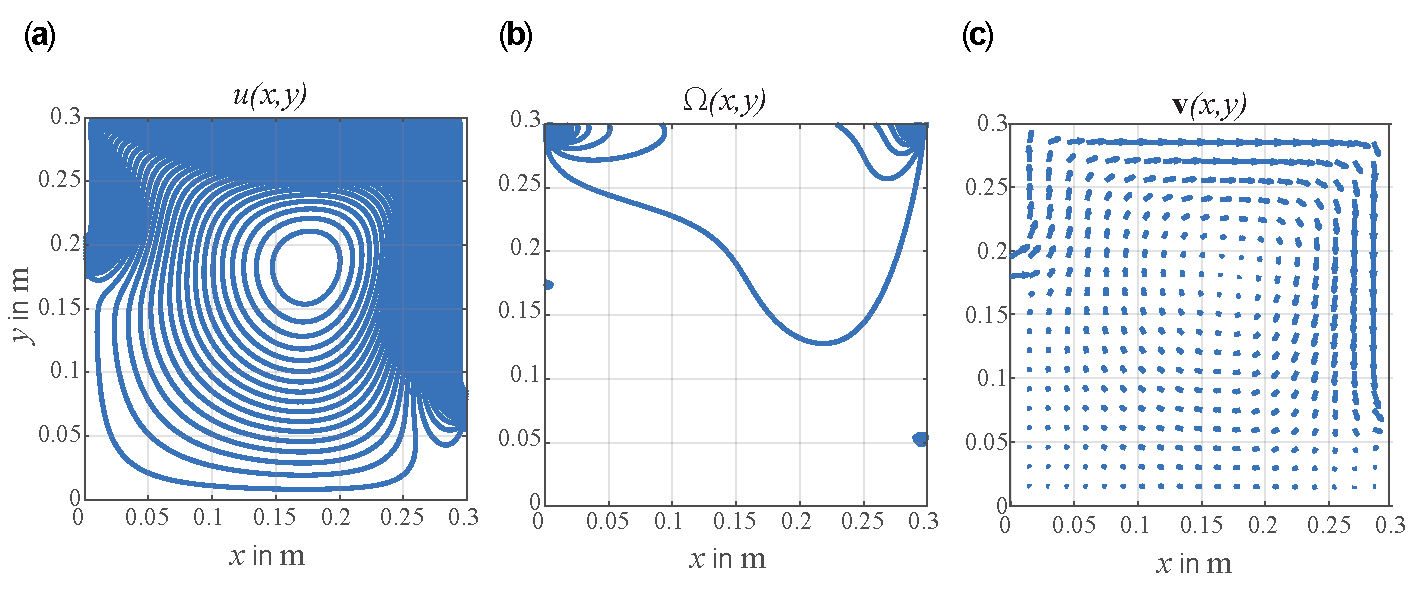
\includegraphics[width=\textwidth]{Tank_Fluss.pdf}
  \caption[Geschwindigkeitsprofil einer Str�mung durch einen Tank.]
  {Geschwindigkeitsprofil der Str�mung durch einen Tank von einem Einflussloch
    links zu einem Ausflussloch rechts. Dargestellt sind \fa die Flusslinien
    (Linien mit konstantem $u$), \fb die Wirbellinien (Linien mit konstantem
    $\Omega$) sowie \fc das Geschwindigkeitsfeld $\vec{v}$ als Vektordiagramm.}
  \label{abb:kontmech_Tank_Fluss}
\end{figure}

Tats�chlich bildet sich ein Strom der Fl�ssigkeit von links nach rechts aus,
die am oberen Rand orientiert ist.
Durch die Viskosit�t bildet sich ein Wirbel aus. Die Fl�ssigkeitsschichten,
die an die Str�mung von links nach rechts angrenzen, werden mitgenommen. Die
Kontinuit�tsgleichung (bzw. die Massenerhaltung) zwingt das Wasser zum
Nachstr�men, sodass sich ein Fluss im Kreis ausbildet.

Die Wirbellinien zeigen, dass der Wirbelvektor sich am st�rksten in den
Ecken �ndert. Dies ist zu erwarten. Bei nahezu parallelen Str�mungen muss
sich mit dem Abstand zur Wand ein Gradient der Geschwindigkeit ausbilden.

Auch hier empfehlen wir dem Leser, die gegenseitige Lage von Eintritts und Austritts�ffnung zu variieren.

\end{sol} 
\textcolor{blue} {$\rightarrow$ zur} \probref{kontmech_StroemungTank}.\\
\noindent\rule[1ex]{\textwidth}{0.5pt}  \newpage  \clearpage
%-----------------------------------------------------------------------------------------------------------

\begin{sol}{prob:kontmech_IdealerWirbel}\label{lsg:kontmech_IdealerWirbel} %�bung13
\textbf{Idealer Wirbel}\\ \\

Der Wirbelvektor \eqref{eq:kontmech_Wirbelvektor}, 
\begin{equation*}
  \vec{\Omega} = \frac{1}{2} \rotv \vec{v} \; ,
\end{equation*}
l�sst sich aus dem Geschwindigkeitsprofil berechnen. Im ersten Fall, dem
Wirbelkern, haben wir eine kreisrunde Rotation mit konstanter
Winkelgeschwindigkeit. Diese ist durch
\begin{equation*}
  \vec{v}_\mathrm{K} = r \omega \, \vec{e}_\varphi
\end{equation*}
gegeben. Damit erh�lt man den Wirbelvektor
\begin{equation*}
  \vec{\Omega}_\mathrm{K} = \frac{1}{2} \rotv \, r \omega\, \vec{e}_\varphi
  = \frac{1}{2} \, \veceZ \frac{1}{r} \frac{\partial}{\partial r} \left ( r^2
    \omega \right ) = \omega \veceZ \; .
\end{equation*}

Im �u�eren Bereich ist die Umlaufgeschwindigkeit konstant, was sich durch
\begin{equation*}
  \vec{v}_\mathrm{A} = v_\varphi \vec{e}_\varphi
\end{equation*}
mit konstantem $v_\varphi$ ausdr�cken l�sst. Der zugeh�rige Wirbelvektor lautet
\begin{equation*}
  \vec{\Omega}_\mathrm{A} = \frac{1}{2} \rotv \, v_\varphi \vec{e}_\varphi
  = \frac{1}{2} \, \veceZ \frac{1}{r} \frac{\partial}{\partial r} \left ( r
    v_\varphi \right ) = \frac{v_\varphi}{2 r} \, \veceZ \; .
\end{equation*}

An beiden Beispielen rechnen wir die Beziehung
\eqref{eq:kontmech_ZirkulationWirbelvektor} nach. Zun�chst tun wir dies
f�r den Wirbelkern. Die direkte Berechnung der Zirkulation aus der
Definition \eqref{eq:kontmech_Zirkulation} entlang des Kreises mir Radius
$R$ ergibt
\begin{equation*}
  Z_\mathrm{K} = \oint_{\partial A} \vec{v}_\mathrm{K} \cdot \D\vec{s}
  = \int_0^{2\pi} R \omega \, R \, \D \, \varphi = 2\pi\, R^2 \omega \; .
\end{equation*}
Nach \eqref{eq:kontmech_ZirkulationWirbelvektor} muss dies identisch sein
mit dem Fl�chenmittelwert des Betrags des Wirbelvektors mal der doppelten
Fl�che, also
\begin{equation*}
  Z_\mathrm{K} = \frac{2A}{A} \int_{A} \left | \vec{\Omega}_\mathrm{K}
  \right | \D A = 2 \int_{A} \left | \vec{\Omega}_\mathrm{K} \right | \D A
  = 2 \int_0^R r \, \D r \, \int_0^{2\pi}\, \D \varphi \, \omega
  = 2\pi\, R^2 \omega \; ,
\end{equation*}
was tats�chlich exakt �bereinstimmt.

F�r den �u�eren Bereich ergibt sich aus der direkten Berechnung
\begin{equation*}
  Z_\mathrm{A} = \oint_{\partial A} \vec{v}_\mathrm{A} \cdot \D\vec{s}
  = \int_0^{2\pi} \, v_\varphi \, R \, \D \, \varphi = 2\pi\, R v_\varphi \; .
\end{equation*}
�ber den Betrag des Wirbelvektors erh�lt man
\begin{equation*}
  Z_\mathrm{A} = 2 \int_{A} \left | \vec{\Omega}_\mathrm{A} \right | \D A
  = 2 \int_0^R r \, \D r \, \int_0^{2\pi}\, \D \varphi \, \frac{v_\varphi}{2 r}
  = 2\pi\, R v_\varphi \; .
\end{equation*}
Auch dies stimmt wieder �berein. Hier muss man jedoch beachten, dass die
Herleitung von \eqref{eq:kontmech_ZirkulationWirbelvektor} davon ausgeht, dass
der funktionale Zusammenhang $\vec{v} = \vec{v}(r,\varphi)$ sich nicht �ndert.
Man muss also im Fl�chenintegral immer die Form annehmen, die im �u�eren
Bereich vorliegt.


\end{sol} 
\textcolor{blue} {$\rightarrow$ zur} \probref{kontmech_IdealerWirbel}.\\
\noindent\rule[1ex]{\textwidth}{0.5pt}  \newpage  \clearpage

%-----------------------------------------------------------------------------------------------------------

\begin{sol}{prob:kontmech_UmformungWirbelsatz}\label{lsg:kontmech_UmformungWirbelsatz} %�bung14
\textbf{Helmholtzscher Wirbelsatz}\\ \\

Zum Beweis der Identit�t
\begin{equation*}
  \rotv \underbrace{\lk \lk \vec{v} \cdot \nablav \rk \vec{v} \rk}_{\vec{A}}
  = \rotv \underbrace{\lk  \rotv \vec{v} \times \vec{v} \rk}_{\vec{A}}
\end{equation*}
beginnen wir mit dem Term auf der linken Seite und subtrahieren die Rotation eines
Gradientenfeldes hinzu, was den Term nicht ver�ndert, da die Rotation
eines Gradientenfeldes immer verschwindet,
\begin{equation*}
  \rotv \lk \lk \vec{v} \cdot \nablav \rk \vec{v} \rk
  = \rotv \lk \lk \vec{v} \cdot \nablav \rk \vec{v} \rk - \rotv \frac{1}{2}
  \nablav (\vec{v}\cdot\vec{v}) \\
  = \rotv \lk \lk \vec{v} \cdot \nablav \rk \vec{v} - \frac{1}{2}
  \nablav (\vec{v}\cdot\vec{v}) \rk = \rotv \vec{A}
\end{equation*}
Den Term in der Klammer dr�cken wir nun in Indexschreibweise (siehe Kap. Mathematische Grundlagen im L�sungsteil)
aus.
\begin{align*}
  \vec{A} & = \lk \vec{v} \cdot \nablav \rk \vec{v} - \frac{1}{2}
  \nablav (\vec{v}\cdot\vec{v}) = \lk \sum_i v_i \frac{\partial}{\partial x_i} \sum_j v_j \vec{e}_j \rk
  - \frac{1}{2} \sum_j \vec{e}_j \frac{\partial}{\partial x_j} \lk
  \sum_i \vec{v}_i \vec{v}_i \rk \\
  &= \sum_i \sum_j \vec{e}_j v_i \frac{\partial v_j}{\partial x_i} 
  - \sum_i \sum_j \vec{e}_j v_i \frac{\partial v_i}{\partial x_j}\,.
\end{align*}
Im n�chsten Schritt f�hren wir zwei Kronecker-Deltas so ein, dass alle
Variablen dieselben Bezeichnungen tragen:
\begin{align*}
  \vec{A} &= \sum_i \sum_j \vec{e}_j v_i \frac{\partial v_j}{\partial x_i} 
  - \sum_i \sum_j \vec{e}_j v_i \frac{\partial v_i}{\partial x_j} \\
  &= \sum_i \sum_j \sum_l \sum_m \delta_{mj} \delta_{li} \vec{e}_j v_i
  \frac{\partial v_m}{\partial x_l} 
  - \sum_i \sum_j \sum_l \sum_m \delta_{mi} \delta_{lj} \vec{e}_j v_i
  \frac{\partial v_m}{\partial x_l} \\
  &= \sum_i \sum_j \sum_l \sum_m \lk \delta_{mj} \delta_{li}
  - \delta_{mi} \delta_{lj} \rk \vec{e}_j v_i \frac{\partial v_m}{\partial x_l} 
  = \sum_i \sum_j \sum_l \sum_m  \epsilon_{kml} \epsilon_{kji}
  \vec{e}_j v_i \frac{\partial v_m}{\partial x_l} \\
  &= - \sum_i \sum_j \sum_l \sum_m  \epsilon_{klm} \epsilon_{kji}
  \vec{e}_j v_i \frac{\partial v_m}{\partial x_l}
  = - \sum_i \sum_j  \epsilon_{kji} \vec{e}_j v_i \lk \nablav \times \vec{v}
  \rk_k \\
  &= - \sum_i \sum_j  \epsilon_{jik} \vec{e}_j v_i \lk \nablav \times \vec{v}
  \rk_k 
  = - \sum_i \sum_j  \epsilon_{jki} \vec{e}_j \lk \nablav \times \vec{v}
  \rk_k v_i = \lk \nablav \times \vec{v} \rk \times \vec{v} = \rotv \vec{v} \times \vec{v} = \vec{A}\,.
\end{align*}
Zusammenfassend erhalten wir also die gesuchte Identit�t.


\end{sol} 
\textcolor{blue} {$\rightarrow$ zur} \probref{kontmech_UmformungWirbelsatz}.\\
\noindent\rule[1ex]{\textwidth}{0.5pt}  \newpage  \clearpage

%-----------------------------------------------------------------------------------------------------------

\begin{sol}{prob:kontmech_fluesse}\label{lsg:kontmech_fluesse} %�bung15
\textbf{Ist der Rhein laminar oder turbulent?}

  \begin{figure}
    \centering
    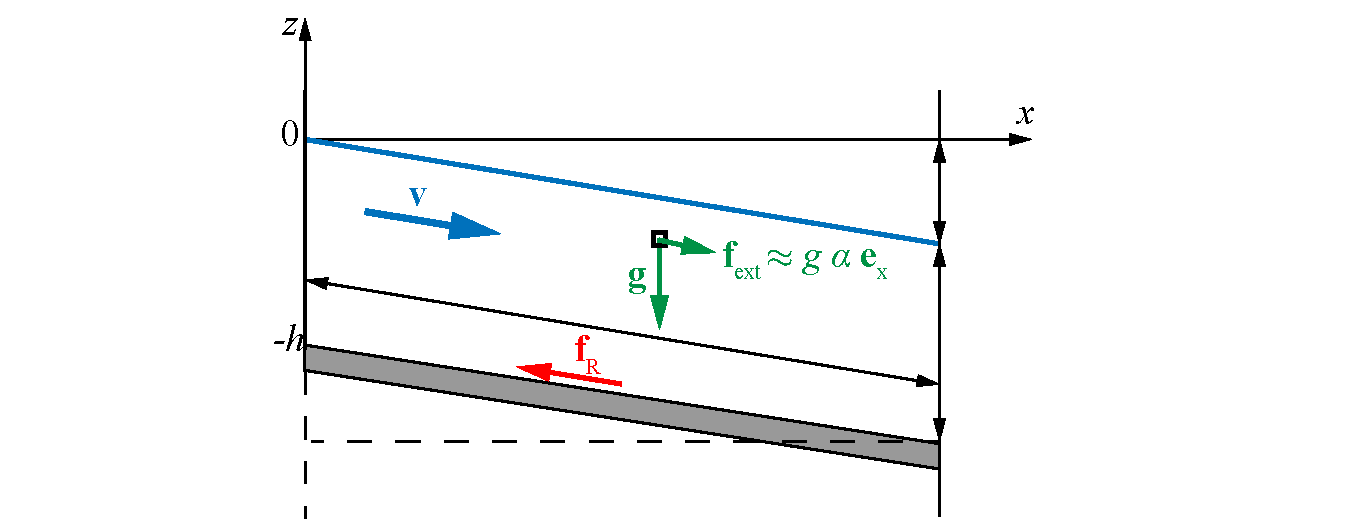
\includegraphics[width=\textwidth]{Flussgefaelle.pdf}
    \caption[Flussgef�lle mit gleichf�rmiger Wasserspiegellage.]
    {Flussgef�lle mit gleichf�rmiger Wasserspiegellage.}
    \label{abb:kontmech_fluesse01}
  \end{figure}

Wir betrachten mit \figref{kontmech_fluesse01} einen Fluss mit einer Tiefe $h$ und einem Gef�lle von 
\begin{align}
    \alpha =   \arctan \frac{\Delta h}{l} \approx \frac{\Delta h}{l} \ll 1\,. \label{eq:kontmech_fluesse01}
\end{align}
Auf ein Volumenelement des Wassers wirkt dann in $x-$-Richtung die externe (Gravitations-) Kraft:
\begin{align}
    \vec{f}_\text{ext} = -\varrho\,g\,\sin\alpha\,\veceX \approx \varrho\,g\,\alpha\,\veceX \,. \label{eq:kontmech_fluesse02}
\end{align}
F�r die inkompressible Fl�ssigkeit nehmen wir ferner an, dass die Breite des Flusses sehr viel gr��er ist als die H�he, sowie das Gef�lle konstant ist, so dass die Ableitungen der Geschwindigkeit nach $y$ und $x$ vernachl�ssigt werden k�nnen. \\
Die \NVS wird dann im laminaren Fall einfach:
\begin{align}
    0 = \vec{f}_r-\vec{f}_\text{ext} =\lk \eta\,\frac{\d^2v_x}{\d z^2}-\varrho\,g\,\alpha\rk\,\veceX\,, \label{eq:kontmech_fluesse03}
\end{align}
mit den Randbedingungen:
\begin{align*}
    z= 0:~~v_x = v_\text{F}~~~\text{\bzw}~~~z = -h:~~v_x = 0\,. 
\end{align*}
Daraus erhalten wir:
\begin{align}
    v\lk z\rk = \frac{1}{2}\,\frac{\varrho\,g\,\alpha}{\eta}\,\lk h^2-z^2\rk ~~~~~~~~0\geq z \geq -h \label{eq:kontmech_fluesse04}
\end{align}
Wir �berpr�fen f�r typische Parameter die Reynoldszahl Re ($h=\SI{2}{\metre}$, $\alpha= \SI{2e-3}{}$, $\eta = \SI{e-3}{\kg\per\metre\per\second}$), indem wir zun�chst $v_\text{F} = \frac{1}{2}\,\varrho\,g\,\alpha\,h^2/\eta$ berechnen. Mit den Parametern w�rden daraus v�llig unrealistische $v_\text{F} = \SI{20e3}{\metre\per\second}$ folgen. Umgekehrt erh�lt man bei einer typischen (schon gro�en) Flussgeschwindigkeit von $\SI{5}{\metre\per\second}$ und einem Volumenstrom (Durchflussrate) von $Q=v\,b\,h\approx \SI{100}{\cubic\metre\per\second}$ ergeben sich eine Reynoldszahl von  $\Re = \varrho\,v\,h/\eta \approx \SI{e6}{}$, 
\dh wir sind in jedem Fall im turbulenten Bereich. Der Ansatz eines laminaren Flusses und einer Reibung nach \eqref{eq:kontmech_fluesse03} ist also zu verwerfen.\\
Man kann nun f�r die Flie�geschwindigkeit $v_\text{F}$ verschiedene (halb) empirische Ans�tze machen, indem man die mittlere Flie�geschwindigkeit $\bar{v}_\text{F}$ des Gew�ssers in Beziehung zu einer Reibungskraft setzt, die sich aus der Turbulenz ergibt. Ein einfacher (Newtonscher) Ansatz f�r die Reibung besteht in:
\begin{align}
    \vec{f}_\text{R} = C\,\varrho\,\frac{\vec{v}_\text{F}{}^2}{h}\,\veceX\,,\label{eq:kontmech_fluesse05} 
\end{align}
worin $C$ ein (halb) empirischer Faktor ist, der die Reibungskraft in Bezug auf die Oberfl�cheneigenschaften des Flussbettes beschreibt. 
Man muss beachten, dass $h$ im Nenner eine Zunahme der Reibung mit geringer Wassertiefe bedeutet!\\
Mit \eqref{eq:kontmech_fluesse03} erh�lt man dann die Formel von Brahms\footnote{Albert Brahms (1692--1758) war ein bedeutender deutscher Deichbaupionier, der bereits 1757 wesentlichen noch heute g�ltige Grundlagen der Deich- und Wasserbaukunst ver�ffentlichte.} 
-Ch�zy\footnote{Antoine de Ch�zy (1718--1798) war ein franz�sischer Hydraulik-Ingenieur.}:
\begin{align*}
    \bar{v}_\text{F,BC} = C\,\sqrt{h\,\alpha\,g}\,.
\end{align*}
Ein anderer Ansatz besteht in der sogenannten Gauckler\footnote{Philippe Gaspard Gauckler (1826--1905) war ein franz�sischer Tiefbauingenieur.}-Manning\footnote{Robert Manning (1816--1897) war ein irischer Ingenieur. Er ver�ffentlichte 1891 die sp�ter unter Gauckler-Manning-Strickler-Flie�formel bekannte Formel in dem Artikel "`On the flow of water in open channels and pipes"' in Irland.}-Strickler\footnote{Albert Strickler (1887--1963) war ein Schweizer Maschinenbau- und Wasserbauingenieur, der durch seine Beitr�ge zur Fluiddynamik bekannt wurde.}\indexp{Brahm, Albert}\indexp{Ch�zy, Antoine de}\indexp{Gauckler, Philippe Gaspard}\indexp{Manning, Robert}\indexp{Strickler, Albert}-Formel. 
\begin{align*}
    \bar{v}_\text{F, GMS} = k_\text{S}\,\sqrt{\alpha}\,\sqrt[3]{h^2}\,.
\end{align*}
Aus der Literatur \cite{Martin2009} findet man f�r die Parameter $C$ \bzw $k_\text{S}$, die im Wesentlichen von der Rauigkeit des Flussbettes abh�ngen f�r Schotter-Werte im Bereich von $C = 20$ \bzw $k_\text{S} = \SI{30}{\per\cubic\metre\per\second}$ liegen. F�r den (turbulenten) Rhein ($\alpha= \SI{2e-4}{}$, $h = \SI{6}{\metre}$) ergibt sich daraus eine mittlere Flie�geschwindigkeit von
\begin{align*}
    \bar{v}_\text{F, BC} \approx \SI{1.52}{\metre\per\second} ~~~~ \text{\bzw} ~~~~ \bar{v}_\text{F, GMS} \approx \SI{1.41}{\metre\per\second}\,,
\end{align*}
was gut mit den beobachteten Geschwindigkeiten �bereinstimmt.\\
Die numerische Behandlung ist nicht trivial und stellt gegen�ber den in \probref{kontmech_StroemungRechteckrohr} \bzw \probref{kontmech_StroemungTank} dargestellten Verfahren, die sich jeweils auf laminare Probleme beziehen, eine nochmalige Komplikation dar. Das Problem ist dabei, dass auf Grund der Turbulenz die einzelnen Str�mungsgr��en (vor allem $\vec{v}\lk \vec{r},t\rk,\, p\lk \vec{r},t\rk$) in ihrem zeitlichen Verlauf und r�umlichen Strukturen nicht aufgel�st werden k�nnen (Speicherbedarf, Rechenkapazit�t).
Man arbeitet daher mit einer modifizierten Form der \NVS, den sogenannten Reynolds-Gleichungen\index{Reynolds-Gleichungen}, bei denen die einzelnen Str�mungsgr��en (\zb $\vec{v},\, p$) durch einen zeitlichen Mittelwert und eine Schwankungsgr��e ausgedr�ckt werden, also:
\begin{align*}
    \vec{v} = \bar{\vec{v}}+\vec{v}' ~~~~ \text{und} ~~~~ p = \bar{p} + p'\,.
\end{align*}
Die Reynoldsgleichungen f�r die inkompressible Fl�ssigkeit folgen dann, wenn man Dichte- und Viskosit�tsschwankungen vernachl�ssigt, \dh
\begin{align*}
    \frac{\d\rho}{\d t} &= 0 \leftrightarrow \rho = \text{const.} ~~~\text{\bzw}~~~
    \frac{\d\eta}{\d t} = 0 \leftrightarrow \eta = \text{const.}
\end{align*}
in Komponentenschreibweise aus der \NVS
\begin{align}
        \rho\,\frac{\d v_i}{\d t} + \rho\,\lk \frac{\d v_i v_j}{\d x_j}\rk &= f_\text{ext,i} - \frac{\d p}{\d x_i} + \eta\,\frac{\d}{\d x_j}\,\lk \frac{\d v_i}{\d x_j} + \frac{\d v_j}{\d x_i}\rk \label{eq:kontmech_reynoldsequ01a}
\end{align} 
zu				
\begin{align}
  \rho\,\frac{\d \bar{v}_i}{\d t} + \rho\,\lk \frac{\d \bar{v}_i \bar{v}_j}{\d x_j}\rk &= \bar{f}_\text{ext,i} - \frac{\d \bar{p}}{\d x_i} + \frac{\d}{\d x_j}\,\lk \eta \lk \frac{\d \bar{v}_i}{\d x_j} + \frac{\d \bar{v}_j}{\d x_i}\rk - \underbrace{\rho\,\overline{v_i'v_j'}}_{\substack{\text{RST}}}\rk\,,
\label{eq:kontmech_reynoldsequ01b}
\end{align} 
wobei $\overline{v_i'v_j'}$ die zeitliche Mittelung �ber die Schwankungsgr��en bedeutet. Die Reynolds-Gleichungen als modifizierte Form der Navier-Stokes-Gleichungen enthalten damit durch die Einf�hrung der Schwankungsterme den sogenannten Reynolds-Spannungstensor RST als zus�tzliche Unbekannte im Gleichungssystem. 
Wir betrachten den RST genauer:
\begin{align}
    -\mathrm{RST}_{ij}=-\sigma_{ij} = \rho\,\overline{v_i'v_j'}= \rho\,
    \begin{pmatrix}
        \:\overline{v_1'\,v_1'}\: & \overline{v_1'\,v_2'}\: & \overline{v_1'\,v_3'}\:\\
        \:\overline{v_2'\,v_1'}\: & \overline{v_2'\,v_2'}\: & \overline{v_2'\,v_3'}\:\\
        \:\overline{v_3'\,v_1'}\: & \overline{v_3'\,v_2'}\: & \overline{v_3'\,v_3'}\:
    \end{pmatrix}\label{eq:kontmech_reynoldsequ02}
\end{align}
Die Diagonalelemente des Tensors stellen Normalspannungen dar, w�hrend die Nichtdiagonal-Elemente Schubspannungen sind.\\
F�r die Berechnung dieser unbekannten Gr��en stehen allerdings nicht mehr Gleichungen zur Verf�gung. Das Gleichungssystem ist \eqref{eq:kontmech_reynoldsequ01b} ist damit nicht mehr geschlossen. Die "`Schlie�ung"' erreicht man durch zus�tzliche Annahmen f�r die Komponenten des Reynolds-Spannungstensors in Form von zus�tzlichen Gleichungen, die im Prinzip Turbulenzmodelle darstellen. Meist beruhen diese semi-empirischen Modellen und werden urch Experimente verifiziert.\\
In den meisten F�llen beruhen die Modelle auf einem Zusammenhangs zwischen den Schwankungstermen und einer gewissen makroskopischen Gr��e $\mu_i$, die als turbulente Viskosit�t bezeichnet wird.\\
Bei den sogenannten Wirbelviskosit�tsmodellen werden die Reynoldsspannungen in Analogie zur �blichen molekulare Viskosit�t $\eta$ hervorgerufenen Spannungen hervorgerufene Spannungen behandelt. Der Reynolds-Spannungstensor lautet folgt approximiert:
\begin{align}
    \rho\,\overline{v_i'v_j'} = -\mu_i\,\lk \frac{\d \bar{v}_i}{\d x_j} + \frac{\d \bar{v}_j}{\d x_i} \rk+ \frac{2}{3}\,\rho\,k\,\delta_{ij}\,.
		\label{eq:kontmech_reynoldsequ03}
\end{align}
Die turbulente Wirbelviskosit�t $\mu$ hat die Dimension $\SI{}{\metre\squared\per\second}$ und beschreibt die Erh�hung der molekularen Viskosit�t durch turbulente Schwankungsbewegungen. In der Regel �berschreitet $\mu$ die molekulare Viskosit�t deutlich. Der Term $\frac{2}{3}\,\rho\,k\,\delta_{ij}$ ist ein \anf{turbulenter Druckterm}, der notwendig ist, um Gleichungen auch f�r Normalspannungen anwenden zu k�nnen (\vgl auch \probref{kontmech_StokesReibung} und \cite{Hoffmann2000}). \\
Mit einem Turbulenzmodell nach \eqref{eq:kontmech_reynoldsequ03} kann die tats�chliche numerische L�sung wie in \probref{kontmech_StroemungRechteckrohr} durch die Finite-Differenzen Methode (FDM) erfolgen. Bei dieser Methode werden die partiellen Differentialgleichungen (Reynolds-Gleichungen) durch Differenzen approximiert und die Unbekannten an den Knotenpunkten mittels Taylor-Reihen ausgedr�ckt. Je nach Genauigkeitsanspruch k�nnen diese bei Gliedern h�herer Ordnung abgebrochen werden. Die partiellen Differentialgleichungen werden auf diese Weise in ein System algebraischer Gleichungen umgeformt \cite{Hoffmann2000, Tu2024}. \\
In der Praxis existiert eine Vielzahl an kommerziellen Softwarepaketen, in denen diese numerischen Verfahren implementiert sind. Diese Anwendung erm�glicht eine relativ \anf{bequeme} Berechnung beziehungsweise Simulation von Str�mungsvorg�ngen verschiedener Fluide. 
FLOW-3D\textregistered\, ist eines dieser Softwarepakete. Mit dessen Hilfe k�nnen viele Problemstellungen der Str�mungsmechanik gel�st werden. Ein Spezialgebiet sind Str�mungen von Fluiden mit freien Oberfl�chen. Wir empfehlen dem interessierten Leser, sich bei \url{www.flow3d.com} \bzw \cite{Tu2024, Hoffmann2000} einen �berblick zu verschaffen.

\end{sol} 
\textcolor{blue} {$\rightarrow$ zur} \probref{kontmech_fluesse}.\\
\noindent\rule[1ex]{\textwidth}{0.5pt}  \newpage  \clearpage
%-----------------------------------------------------------------------------------------------------------

\begin{sol}{prob:kontmech_StokesReibung}\label{lsg:kontmech_StokesReibung} %�bung16
\textbf{Stokes-Reibung}\index{Stokes-Reibung}\\ \\

Es gibt verschiedene Herleitungen der Stokes-Formel\footnote{Sir George Gabriel Stokes\indexp{Stokes, Sir George Gabriel} (1819--1903) war ein irischer Mathematiker und Physiker. Er arbeitete auf dem Gebiet der mathematischen und experimentellen Physik und besch�ftigte sich haupts�chlich mit der Hydrodynamik, der Elektrodynamik und der Akustik.Seine ber�hmte Formel ver�ffentlichte er erstmalig 1851 unter dem Titel "'On the effect of the internal friction of fluids on the motion of pendulums."' in den Transactions of the Cambridge Philosophical Society, Band 9, 1861, S. 8�106.}. Wir folgen hier im wesentlichen der exzellenten Darstellung in \cite{Schmutzer2005} folgen, die wir durch eine Plausibilit�tsbetrachtung, einen Einschub zum Spannungstensor und numerische Rechnungen erg�nzen.\\

\textbf{Absch�tzung, Plausibilit�tsbetrachtung}\\

Wir wollen zun�chst mit Hilfe von \figref{kontmech_stokesformel01} eine Absch�tzung treffen. Wir betrachten eine station�r flie�ende, inkompressible z�he Fl�ssigkeit ohne �u�ere Kr�fte, in der sich eine Kugel befindet. Im gro�en Abstand von der Kugel mit dem Radius $R_0$ hat die Str�mung eine konstanten Geschwindigkeit $\vec{v}_0 = v_0 \,\veceX$, auf der Kugeloberfl�che ist die Geschwindigkeit Null.  Wir k�nnen davon ausgehen, dass in einer Entfernung von $\approx\,R_0$ von der Kugeloberfl�che die Geschwindigkeit $\vec{v}_0$ nahezu wieder erreicht, was einem Geschwindigkeitsgradient von ungef�hr $\vec{v}_0/R_0$ entspricht. Nach \eqref{eq:kontmech_ReibungskraftInnere} entspricht das einer inneren Reibungskraft, die sich mit der Viskosit�t $\eta$ als Proportionalit�tsfaktor 
zu \begin{equation}
  \vec{F}_\text{R} \approx \eta \, A \, \frac{\partial v_z}{\partial y} \veceZ \approx \eta \, 4 \pi R_0{}^2 \,\frac{v_0}{R_0} \veceZ \approx  4\pi R_0{} v_0 \veceZ \;
  \label{eq:kontmech_kontmech_stokesformel_approx}
\end{equation}
ergibt. Das ist schon mal die richtige Gr��enordnung, wir werden im Folgenden sehen, dass die genaue Ber�cksichtigung der Geometrie bei der L�sung der \NVS{} einen 1.5 mal gr��eren Wert der Kraft ergibt.

  \begin{figure}
    \centering
    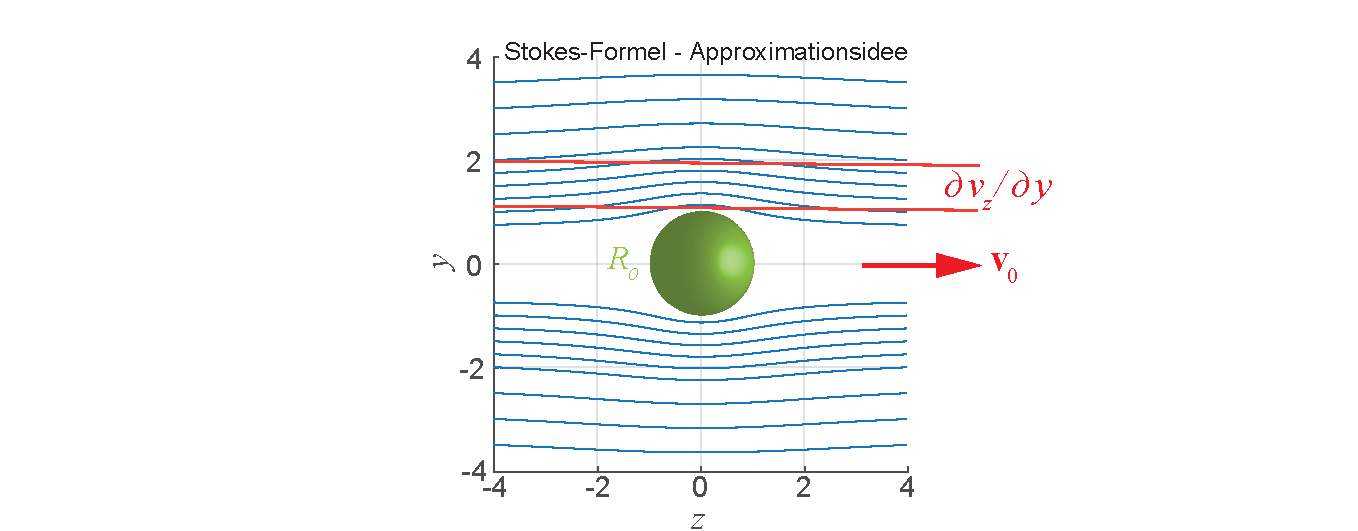
\includegraphics[width=\textwidth]{StokesFormel01.pdf}
    \caption[Geschwindigkeitsprofil einer viskosen Str�mung um eine Kugel (N�herung).]
    {Geschwindigkeitsprofil einer viskosen Str�mung um eine Kugel (N�herung).}
				\label{abb:kontmech_stokesformel01}
  \end{figure}

\textbf{Berechnung des Geschwindigkeitsfeldes aus der f�r den Stokes-Fall vereinfachten \NVS}\\

Neben der Kontinuit�ts- \bzw Inkompressibilit�tsgleichung \eqref{eq:kontmech_KontinuitaetsglInkompr} 
\begin{align}     
\divv\,\vec{v} = 0 ~~~~~~~~~ \text{mit}~~~ \varrho = \varrho_0 = \con \label{eq:kontmech_Stokes01} 
\end{align} 
ist also die Navier-Stokes-Gleichung \eqref{eq:kontmech_NavierStokesFrei}
\begin{align}   \varrho_0\,\lk\vec{v}\,\nablav\rk\,\vec{v} = -\gradv \,p + \eta\,\Delta\,\vec{v} \label{eq:kontmech_Stokes02}
\end{align} 
zu l�sen, wobei die Randbedingungen folgenderma�en lauten: 
\begin{align} ~~~~ \vec{v}(r~\rightarrow~\infty) = \vec{v}_0 = v_0\, \veceZ ~~~~~\text{und}~~~~~ \vec{v}(r~\rightarrow~R_0)= 0\,. \label{eq:kontmech_Stokes03} 
\end{align} 
Die zweite Randbedingung bringt das Haften der Fl�ssigkeit an der Kugeloberfl�che zum Ausdruck (no slip).\\

Wir linearisieren die \NVS{} unter der Annahme kleiner Reynolds-Zahlen, \dh 
$ \Re = \varrho_0 R_0 v_0\,/\,\eta_0 \,\ll\,1\,.$ Wir erhalten dann aus \eqref{eq:kontmech_Stokes02} 
\begin{align}     
\Delta\, \vec{v} = \frac{1}{\eta}\,\gradv \,p ~~~\text{und}~~~
  \rotv \lk \Delta \vec{v}\rk = 0\,. \label{eq:kontmech_Stokes05}
\end{align} 
Einen L�sungsansatz f�r die zweite Gleichung ist durch
\begin{align}     
 \vec{v} = \gradv \,\Psi + \bar{\vec{v}} ~~~~~~ \text{mit} ~~~ \Delta \bar{\vec{v}} = 0\,. \label{eq:kontmech_Stokes06} 
\end{align} 
gegeben.\footnote{Man beachte dabei die Vertauschbarkeit der partiellen Ableitungen.} Unter Ber�cksichtigung der Randbedingungen l�sen wir \eqref{eq:kontmech_Stokes06} f�r $r\neq 0$ durch 
\begin{align}     
\bar{\vec{v}} = \vec{v}_0\,\frac{A}{r} \,, \label{eq:kontmech_Stokes07} 
\end{align} 
worin $A$ eine Integrationskonstante ist.
Mit \eqref{eq:kontmech_Stokes01} folgt aus \eqref{eq:kontmech_Stokes06} 
\begin{align}     
\Delta\Psi = -\divv\,\bar{\vec{v}} = -A\,\vec{v}_0\,\gradv\lk\frac{1}{r}\rk = \frac{A}{r^2}\lk \vec{v}_0\,\vec{e}_r\rk  = \frac{A}{r^3}\lk \vec{v}_0\,\vec{r}\rk \,. \label{eq:kontmech_Stokes09} 
\end{align} 
Wir suchen nun eine L�sung dieser inhomogenen Differentialgleichung f�r $\Psi$. Wir versuchen den Ansatz \begin{align}    
\Psi = \lk \vec{v}_0\,\vec{r}\rk\,\Phi\lk r\rk\,,\label{eq:kontmech_Stokes10} 
\end{align} 
aus dem sich 
\begin{align}     
 \gradv\Psi = \lk \vec{v}_0\,\vec{r}\rk \,\gradv\Phi +\vec{v}_0\,\Phi ~~~~~~\text{und} ~~~~ \Delta\Psi = \lk \vec{v}_0\,\vec{r}\rk\,\Delta \Phi +2\vec{v}_0\,\gradv \Phi 
\label{eq:kontmech_Stokes11} 
\end{align} 
ergeben. Mit \eqref{eq:kontmech_Stokes09} erhalten wir die gew�hnliche inhomogene Differentialgleichung 
\begin{align}     
\Delta \Phi +\frac{2\vec{r}}{r^2}\,\gradv \Phi = \frac{A}{r^3} ~~~~ \text{\bzw} ~~~~~ \Phi'' +\frac{4}{r}\,\Phi' = \frac{A}{r^3}\,. \label{eq:kontmech_Stokes12} 
\end{align} 
Dabei bedeutet $\Phi'$ die Ableitung nach $r$ (Kugelkoordinate). Die homogene Differentialgleichung l�sen wir mit dem Potenzansatz 
\begin{align}     \Phi^{\lk h\rk} = r^\lambda\,, \label{eq:kontmech_Stokes13} 
\end{align} 
der auf $\lambda^2 + 3\lambda = 0$ und damit $\lambda_1 = 0\,, ~~\lambda_2 = -3$ f�hrt. F�r die L�sung der inhomogenen Gleichung ergibt sich
\begin{align}     
\Phi^{\lk \text{inh}\rk} = -\frac{A}{2r}\,, \label{eq:kontmech_Stokes14} 
\end{align} 
und damit folgt die allgemeine L�sung zu 
\begin{align}     \Phi = a + \frac{b}{r^3} - \frac{A}{2r} \,, \label{eq:kontmech_Stokes15} 
\end{align} 
worin $a,\,b\,$ Integrationskonstanten sind. 
�ber \eqref{eq:kontmech_Stokes10} und \eqref{eq:kontmech_Stokes06} ergibt sich damit f�r f�r das Geschwindigkeitsfeld:
\begin{align}     
\vec{v} = \frac{\vec{r}\,\lk \vec{v}_0\,\vec{r}\rk}{r^3}\,\lk -\frac{3b}{r^2}+\frac{A}{2}\rk + \vec{v}_0\,\lk a+\frac{b}{r^3} + \frac{A}{2r}\rk \,. \label{eq:kontmech_Stokes16} 
\end{align} 

Die Erf�llung der ersten Randbedingung liefert $a=1$ und aus der zweiten ergibt sich
\begin{align}     
\frac{\vec{r}_0\,\lk \vec{v}_0\,\vec{r}_0\rk}{R_0{}^3}\,\lk \frac{A}{2} - \frac{3b}{R_0{}^2}\rk + \vec{v}_0\,\lk 1 +\frac{b}{R_0{}^3} +\frac{A}{2R_0}\rk = 0 \,, \label{eq:kontmech_Stokes17} 
\end{align} 
wobei $\vec{r}_0$ der auf die Kugeloberfl�che zeigende winkelabh�ngige Radiusvektor ist. Aus dieser Gleichung folgt das Verschwinden der Koeffizienten 
\begin{align}     \frac{A}{2} - \frac{3b}{R_0{}^2} = 0~~~~\text{und}~~~~~ 1+\frac{b}{R_0{}^3} + \frac{A}{2R_0} = 0\,, \label{eq:kontmech_Stokes18} 
\end{align} 
da die Gleichung f�r alle $\vec{r}_0$ gelten muss. Die Aufl�sung dieser beiden Gleichungen ergibt 
\begin{align}     
A= -\frac{3R_0}{2}\,, ~~~~ b=-\frac{R_0{}^3}{4}\,, \label{eq:kontmech_Stokes19} 
\end{align} 
so dass sich das Geschwindigkeitsfeld  \eqref{eq:kontmech_Stokes16} endg�ltig als 
\begin{align}     
\vec{v} = \vec{v}_0\,\lek 1-\frac{R_0}{4r}\,\lk 3 + \frac{R_0{}^2}{r^2}\rk\rek -\vec{e}_r\,\frac{3R_0\,\lk \vec{v}_0\,\vec{e}_r\rk}{4r}\,\lk 1-\frac{R_0{}^2}{r^2}\rk \label{eq:kontmech_Stokes20} 
\end{align} 
schreiben l�sst. Man beachte, das $\vec{e}_r = \sin\vartheta\,\veceY + \cos\vartheta\,\veceZ$ ist mit $\vartheta = \arctan(y/z)$.\\ 

  \begin{figure}
    \centering
    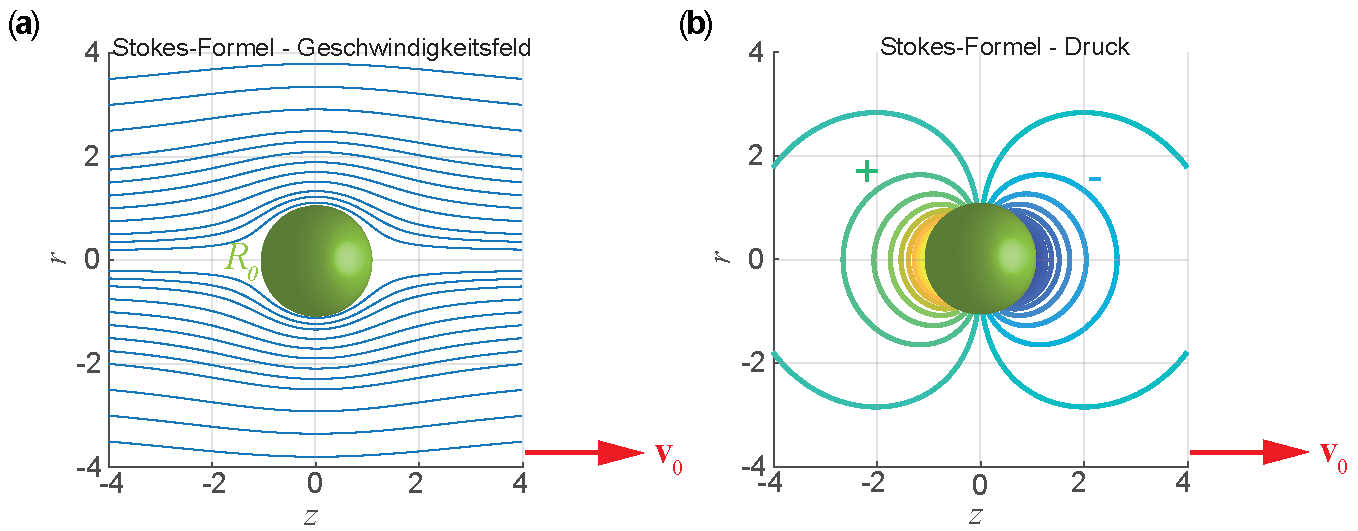
\includegraphics[width=\textwidth]{StokesFormel02.pdf}
    \caption[\fa Geschwindigkeitsprofil und \fb Druck einer viskosen Str�mung um eine Kugel.]
    {Geschwindigkeitsprofil und Druck einer viskosen Str�mung um eine Kugel.}
				\label{abb:kontmech_stokesformel02}
  \end{figure}

Die Auswertung von \eqref{eq:kontmech_Stokes20} ist in \figref{kontmech_stokesformel02} als das Geschwindigkeitsfeld \vec{v}(z,y) dargestellt (siehe auch \mscr{} \mlkontmechref{StokesReibung01.m}).\\

\textbf{Berechnung des Drucks aus dem Geschwindigkeitsfeld}\\

Den Druck kann man aus dem Geschwindigkeitsfeld �ber \eqref{eq:kontmech_Stokes06} aus \eqref{eq:kontmech_Stokes05} berechnen:
\begin{align}     
  \gradv p &= \eta\,\Delta \vec{v} = \eta\,\gradv\lk \Delta\Psi\rk~~\rightarrow~~ p &= p_0 +\eta\,\Delta\Psi \,. \label{eq:kontmech_Stokes21} 
\end{align} 
Wir �berlassen dem Leser die Differentiation, wobei wiederum vorteilhaft die Symbolic Toolbox von \matlab{} benutzt werden kann. Wir geben hier nur das Ergebnis an (siehe auch \figref{kontmech_stokesformel02}).
\begin{align}     
    p &= p_0 - \frac{3}{2}\frac{\eta\,v_0\,R_0\,z}{r^3}\,. \label{eq:kontmech_Stokes_pressure} 
\end{align} 


\textbf{Berechnung der Kraft}\\

Neben dem Druck ben�tigen wir zur Kraftberechnung auch den sogenannten Spannungstensor $\mathbb{T}$. den wir kurz einf�hren wollen (\figref{kontmech_stokesformel03}). Wir k�nnen hier nur eine (f�r den Umfang der �bungsaufgabe hinreichende) Zusammenfassung geben und verweisen den interessierten Leser auf die Literatur, insbesondere \cite{Garvin2023, Schmutzer2005, Bartelmann2015, Hoffmann2000}.

 \begin{figure}
    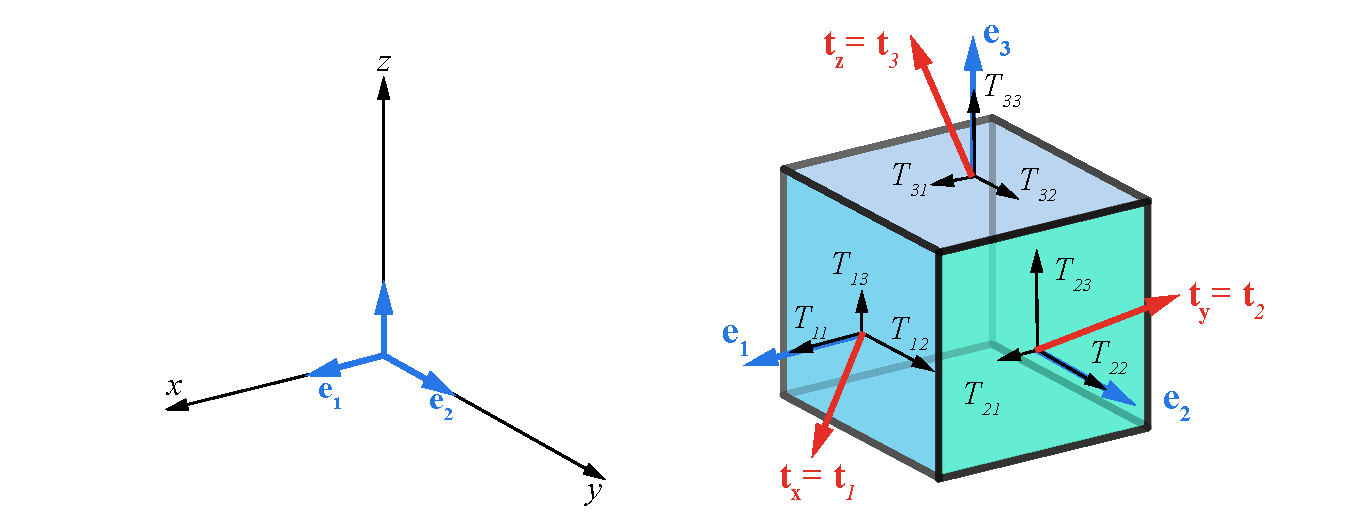
\includegraphics[width=\textwidth]{Spannungstensor.pdf}
    \caption[Komponentendarstellung des Spannungstensors.]
    {Komponentendarstellung des Spannungstensors $T_{ij}$.}
    \label{abb:kontmech_stokesformel03}
  \end{figure}

%Einschub*****************************************************************************************************************

\begin {infobox} {Der Spannungstensor}\index{Spannungstensor}

Bei der Herleitung der 
\begin{itemize}
	\item Euler-Gleichung \eqref{eq:kontmech_EulerGleichung} in \kap{kontmech_EulerGl},
	\item der inneren Reibung in \kap{kontmech_InnereReibung} und daraus folgend der 
	\item der \NVS{} \eqref{eq:kontmech_NavierStokes} in \kap{kontmech_NavierStokes}
\end{itemize}
hatten wir teilweise implizit die Annahme gemacht, dass die Grenzfl�chenkr�fte (auch Spannungsvektoren $\vec{t}_i$ genannt) senkrecht auf den Grenzfl�chen stehen bzw. in der Grenzfl�che liegen (innere Reibung). Wir wollen das nun etwas verallgemeinern und betrachten einen infinitesimal kleinen W�rfel, bei dem jeweils zwei Fl�chen in $x$-, $y$- und $z$-Richtung orientiert sind. Die Orientierung dieser Fl�chen ist gegeben durch den sogenannten Normalenvektor $\vec{e}_\text{n}$, der positiv sein soll, wenn er in Koordinatenrichtung zeigt.
Wir wollen nun zulassen, dass die Spannungsvektoren $\vec{t_x},\, \vec{t_y}$ und $\vec{t_z}$ beliebig zur Fl�che stehen k�nnen (\figref{kontmech_stokesformel03}). Der Spannungstensor $\mathbb{T}$ ist nun die Gr��e, die die Richtung der Kraft mit der Normalenrichtung verkn�pft, also:
\begin{align}     
    \D \vec{F} &= \D A\,\vec{t}\,= \,\D A \,\mathbb{T}\,\vec{e}_\text{n}  ~~~~\text{\bzw}~~~\D \vec{F}_i = \,\D A\, T_{ij}\, e_{\text{n}j} \,. \label{eq:kontmech_Stokes_einschub01} 
\end{align} 
Der Spannungstensor $\mathbb{T}$ \bzw $T_{ij}$ ist ein Tensor zweiter Stufe und fasst die Normalspannungen in Normalenrichtung, sowie tangential wirkende (transversale) Spannungen (auch Scherspannungen genannt) zu einem mathematisch-physikalischen Objekt zusammen. Die Komponenten des Spannungstensors haben die Dimension eines Drucks. Die Komponenten des Spannungstensors k�nnen wir schreiben als.
\begin{align}     
 \mathbb{T}=\left(\vec{t_x},\ \vec{t_y},\ \vec{t_z}\right)=\left(\begin{matrix}T_{xx}&T_{xy}&T_{xz}\\T_{yx}&T_{yy}&T_{yz}\\T_{zx}&T_{zy}&T_{zz}\\\end{matrix}\right) ~~~~\text{\bzw}~~~~~
T_{ij}=\left(\begin{matrix}T_{11}&T_{12}&T_{13}\\T_{21}&T_{22}&T_{23}\\T_{31}&T_{32}&T_{33}\\ \end{matrix}\right) \,.
	\label{eq:kontmech_Stokes_einschub03} 
\end{align}  
%\begin{align}   
%=\left(\begin{matrix}T_{xx}&T_{yx}&T_{zx}\\T_{xy}&T_{yy}&T_{zy}\\T_{xz}&T_{yz}&T_{zz}\\\end{matrix}\right)   
%=\left(\begin{matrix}T_{11}&T_{21}&T_{31}\\T_{12}&T_{22}&T_{32}\\T_{13}&T_{23}&T_{33}\\\end{matrix}\right) 
	%\label{eq:kontmech_Stokes_einschub04} 
%\end{align} 
Die Indizierung der einzelnen Komponenten folgt dabei einem einfachen Schema: Der erste Index $i$ von $T_{ij}$ steht f�r die Richtung der einzelnen Spannungs- \bzw Kraftkomponente. Der zweite Index $j$ steht f�r die Richtung des Normalenvektors. Betrachten wir also $T_{13}$, dann beschreibt dieser Wert die Spannung der $x$-Komponente zur Fl�che, deren Normalenvektor in $z$-Richtung zeigt. Der Tensor ist symmetrisch, \dh $T_{ij} = T_{ji}$, was eine Folge der Drehimpulserhaltung ist \cite{Garvin2023, Schmutzer2005}.\\
Mit dem Spannungstensor schreibt sich die gesamte Fl�chenkraft �ber eine beliebige Oberfl�che
\begin{align}
    \vec{F}_n =  \oint\limits_{\text{Ar}}\,\hat{T}\,\vec{e}_n\,\D A\,, 	\label{eq:kontmech_Stokes_Gesamtkraft} 
\end{align}
woraus mit dem Gau�-Satz folgt:
\begin{align}
    \vec{F}_\text{g} =  \oint\limits_{\text{Ar}}\,\mathbb{T}\,\vec{e}_n\,\D A +\int\limits_{\text{v}_0} \vec{f}_\text{ext} \D V = \int\limits_{\text{v}_0} \divv\,\mathbb{T}\,\D V\, + \vec{f}_\text{V} \,. \label{eq:kontmevh_einschub07}
\end{align}
Wir erhalten somit die allgemeine Bewegungsgleichung f�r ein Fluid  (eigentlich f�r jedes Kontinuum):
\begin{align}     
    \varrho \lk \lk \vec{v} \cdot \nablav \rk \vec{v} + \frac{\partial}{\partial t} \vec{v} \rk \D \vec{F} &= \gradv \cdot \mathbb{T} + \vec{f}_\text{V} \,. 
		\label{eq:kontmech_Cauchy}
\end{align} 
Diese wurde erstmalig von Cauchy\footnote{Augustin-Louis Cauchy (1789--1857) war ein franz�sischer Mathematiker und lieferte fundamentale Beitr�ge zur Analysis und insbesondere auch zur Gruppen- und Funktionentheorie. In der Physik begr�ndete er die modernen Grundlagen der Kontinuumstheorie. Er war in seiner Bedeutung vergleichbar mit dem in Deutschland wirkenden Carl Friedrich Gau�.}\indexp{Cauchy, Augustin-Louis} aufgestellt wurde und besagt, dass die Bewegungs�nderung eines Fluids durch innere und �u�ere Kr�fte hervorgerufen wird, wobei die ersteren sich als Gradient aus dem Spannungstensor ergeben.\footnote{Wir verweisen auf die �hnlichkeit mit der Ableitung der Kraft aus einem Potential f�r die Bewegung eines Massenpunktes.}

%\begin{align}
    %\varrho\,\lek \frac{\d \vec{v}}{\d t} + \lk \vec{v}\,\nablav\,\vec{v}\rek = \vec{f}_\text{ext} + \nablav\,\mathbb{T}\,. 
%\end{align}
Wie ist nun der Spannungstensor aufgebaut? Er besteht aus 3 Anteilen.
\begin{align}
    \mathbb{T} = \mathbb{T}^{\text{(Druck)}} + \mathbb{T}^{\text{(Volumen)}} + \mathbb{T}^{\text{(Viskos)}}\,. \label{eq:kontmech_einschub08}
\end{align}
$\mathbb{T}^{\text{(Druck)}}$ beschreibt die Spannung in einem Fluid, auch wenn dieses keine Bewegung zeigt, das ist genau der Druck:
\begin{align}
    \mathbb{T}^{\text{(Druck)}} = -p\,\mathbb{I} = 
    \begin{pmatrix}
        -p & 0 & 0\\
        0 & -p & 0\\
        0 & 0 & -p
    \end{pmatrix}\,,  \label{eq:kontmech_einschub09}
\end{align}
worin $\mathbb{I}$ der Einheitstensor ist. $\mathbb{T}^{\text{(Volumen)}}$ beschreibt die Spannung in einem Fluid, die durch Volumen�nderung des Fluids entsteht. Logischerweise verschwindet dieser Anteil, wenn die Fl�ssigkeit inkompressibel ist. 
\begin{align}
    \mathbb{T}^{\text{(Volumen)}} = \lambda\,\lk \nablav\,\vec{v}\rk\,\mathbb{I} = 
    \begin{pmatrix}
        \frac{\d v_i}{\d x_i} & 0 & 0\\
        0 & \frac{\d v_i}{\d x_i} & 0\\
        0 & 0 & \frac{\d v_i}{\d x_i}
    \end{pmatrix}\,,  \label{eq:kontmech_einschub09a}
\end{align}
worin wir wieder die Einsteinsche Summenkonvention benutzt haben. Der Proportianalit�tsfaktor $\lambda$ ist die sogenannte Volumenviskosit�t\index{Volumenviskosit�t} oder auch 2. Koeffizient der Viskosit�t genannt. Sie hat die Einheit $\SI{}{\pascal\second}$.\\
Der dritte Term des Spannungstensors beschreibt schlie�lich die durch innere Reibung hervorgerufenen Spannungen. Man k�nnte vermuten nach Behandlung der Reibungskr�fte im \kap{kontmech_InnereReibung}diesen als $\nablav\,\vec{v}$ zu definieren. Dann w�rde der Spannungstensor aber nicht mehr symmetrisch sein, weswegen der viskose Term folgenderma�en definiert wird:
\begin{align}
\begin{split}
    \mathbb{T}^{\text{(Viskos)}} &= \eta\,\lk \nablav\,\vec{v}+\lk\nablav\,\vec{v}\rk^\intercal\rk \\
    &= 
    \begin{pmatrix}
        2\eta\,\frac{\d v_x}{\d x} & \eta\,\lk \frac{\d v_x}{\d x} + \frac{\d v_x}{\d y}\rk & \eta\,\lk \frac{\d v_z}{\d x} + \frac{\d v_x}{\d z}\rk\\
        \eta\,\lk \frac{\d v_x}{\d y} + \frac{\d v_y}{\d x}\rk & 2\eta\,\frac{\d v_y}{\d y} & \eta\,\lk \frac{\d v_z}{\d y} + \frac{d v_y}{\d z}\rk\\
        \eta\,\lk \frac{\d v_x}{\d z} + \frac{\d v_z}{\d x}\rk & \eta\,\lk \frac{\d v_y}{\d z} + \frac{\d v_z}{\d y}\rk & 2\eta\,\frac{\d v_z}{\d z}
    \end{pmatrix}\,,  
\end{split}   \label{eq:kontmech_Stokes_viskoserT} 
\end{align}
$\eta$ ist die dynamische Viskosit�t \bzw der erste Koeffizient der Viskosit�t. Damit kann der Gesamtspannungstensor in Indexschreibweise geschrieben werden als:
\begin{align}
    T_{ij} = -p\,\delta_{ij} + \lambda\,\lk\frac{\d v_k}{\d x_k}\rk\,\delta_{ij} + \eta\,\lk \frac{\d v_i}{\d x_j} + \frac{\d v_j}{\d x_i}\rk\,.\label{eq:kontmech_einschub11a}
\end{align}
F�r inkompressible Fl�ssigkeiten ist $\lambda=0$ und wir erhalten 
\begin{align}
    T_{ij}= -p\,\delta_{ij} + 2\eta\,\lk \frac{1}{2}\,\frac{\d v_i}{\d x_j} + \frac{\d v_j}{\d x_i}\rk\,,\label{eq:kontmech_einschub12}
\end{align}
woraus mit \eqref{eq:kontmech_Cauchy} eingesetzt, die uns bekannte \NVS{} \eqref{eq:kontmech_NavierStokes} aus \kap{kontmech_NavierStokes} folgt. F�r sogenannte Newton-Fl�ssigkeiten gilt \ia der folgende n�herungsweise g�ltige Zusammenhang:
\begin{align}
    \lambda = -\frac{2}{3}\,\eta\,, \label{eq:kontmech_einschub13}
\end{align}
womit wir eine allgemeinere Form der \NVS{} erhalten:
\begin{align}
    \varrho\,\lek \frac{\vec{v}}{\d t} + \lk \vec{v}\,\nablav\rk\,\vec{v}\rek =  \vec{f}_\text{ext} - \nablav\,\lk \frac{2}{3}\,\eta\,\lk \nablav\,\vec{v}\rk\rk + \nablav\,\lk \eta\lk \nablav\,\vec{v}\rk + \lk \nablav\,\vec{v}\rk^\intercal\rk\,. \label{eq:kontmech_einschub14}
\end{align}


\end{infobox}
% Ende Einschub*************************************************************************************** 
\medskip

Zur�ck zur Herleitung der Kraft f�r den Fall einer Kugel in einer viskosen Str�mung. Wir brauchen den nach \eqref{eq:kontmech_Stokes21} berechneten Druck und den viskosen Spannunsgtensor \eqref{eq:kontmech_Stokes_viskoserT}. Dieser lautet in unserem Fall, da wir Inkompressibilit�t und damit $\lambda=0$ voraussetzen: %wegen \eqref{eq:kontmech_Stokes01}
\begin{align}     
  T_{ij}^{\lk \text{visk} \rk} = \eta\,\lk \frac{\d v_{i}}{x_j} +  \frac{\d v_{j}}{x_i} \rk\,. \label{eq:kontmech_Stokes22} 
\end{align} 

Der Gesamtspannungstensor lautet dann
\begin{align}     
T_{ij}  =  T_{ij}^{\lk \text{visk}\rk} + T_{ij}^{\lk \text{p}\rk} = \eta\,\lk \frac{\d v_{i}}{x_j} +  \frac{\d v_{j}}{x_i} \rk - \lk p_0 +\eta\,\Delta\Psi\rk\,\delta_{ij}\,. \label{eq:kontmech_Stokes23} 
\end{align} 
F�r die auf die Kugel wirkende Kraft ergibt sich mit \eqref{eq:kontmech_Stokes_Gesamtkraft} zu:
\begin{align} 
\begin{split}     
   \vec{F}^{\lk \d \text{K}\rk} &= \vec{e}_i F_i^{\lk \d \text{K} \rk} = \vec{e}_i\int\limits_{\d \text{K}} T_{ij} \,\D A_j  = \eta\,\lek \underbrace{\vec{e}_i \int\limits_{\d \text{K} }\,\eta\,\lk \frac{\d v_{i}}{x_j} +  \frac{\d v_{j}}{x_i} \rk\,\D A_j}_{I_1} -\underbrace{\int\limits_{\d \text{K}}\Delta\Psi\,\D\vec{A}}_{I_2}\rek\,. 
		\label{eq:kontmech_Stokes24} 
\end{split} 
\end{align} 
Im folgenden wollen wir die beiden auftretenden Integrale einzeln berechnen, wobei wir die Fl�chenelemente der Kugelfl�che in Polarkoordinaten verwenden:
\begin{align*}     
  \D\vec{A} = \vec{n}\,\D A = \vec{e}_r\,\D A_r ~~ \text{mit} ~~~~\D A_r = R_0{}^2\,\sin\theta\,\D\phi\,\D \theta\,.
\end{align*} 

\begin{enumerate}
\item  [1)] \textbf{Zwischenrechnung f�r Integral} $I_1$\\ 

Wir schreiben: 
\begin{align}
    I_1 = \vec{e}_i \int\limits_{\lk \d \text{K}\rk} \lk \frac{\d v_i}{\d x_j} + \frac{\d v_j}{\d x_i}\rk\,\D A_j = \int\limits_{\lk \d \text{K}\rk} \lk \frac{\d \vec{v}}{d x_j} + \vec{e}_i\,\frac{\d v_j}{\d x_i}\rk \,\D A_j  = \int\limits_{\lk \d \text{K}\rk}\,\lk \frac{\d \vec{v}}{\d r} + \gradv v_r \rk\,\D A_r\,.
\label{eq:kontmech_Stokes25}
\end{align}
Aus dem Geschwindigkeitsfeld \eqref{eq:kontmech_Stokes20} erhalten wir die Beziehungen
\begin{subequations}
\begin{align}
    \vec{v}_0\,\vec{e}_r &= v_0\,\veceZ\,\vec{e}_r = v_0\,\cos\theta\,,\label{eq:kontmech_Stokes26a}\\
    v_r = \vec{v}\,\vec{e}_r &= v_0\,\cos\theta\,\lek 1-\frac{R_0}{2r}\,\lk 3-\frac{R_0{}^2}{r^2}\rk\rek\,.\label{eq:kontmech_Stokes26b}
\end{align}\label{eq:kontmech_Stokes26}
\end{subequations}
F�r die Kugeloberfl�che $\d \text{K}$ berechnet man aus \eqref{eq:kontmech_Stokes20} und \eqref{eq:kontmech_Stokes26b}:
\begin{enumerate}
    \item [a)] \begin{align}
    \frac{\d \vec{v}}{\d r} \,\Big\vert_{r=R_0} &= \frac{3}{2R_0}\,\lek \vec{v}_0 - \vec{0} - \vec{e}_r\,\lk \vec{v}_0\,\vec{e}_r\rk\rek = \frac{3}{2R_0}\,\vec{e}_r \times \lk \vec{v}_0 \times \vec{e}_r\rk = \frac{3}{2R_0} \,\lk \vec{v}_0 - \vec{e}_r\,v_0\,\cos\theta\rk \nonumber \\
    &= \frac{3v_0}{2R_0}\,\lek -\veceX\,\cos\phi\,\sin\theta\,\cos\theta - \veceY\,\sin\phi\,\sin\theta\,\cos\theta + \veceZ\,\sin^2\theta\rek\,\label{eq:kontmech_Stokes27}
\end{align}
    \item [b)] 
    \begin{align}
        \lk\gradv v_r\rk \Big\vert_{r= R_0}  = 0\,.  \label{eq:kontmech_Stokes27a}
    \end{align}
\end{enumerate}
Damit bekommen wir
\begin{align}
    I_2 &= \,\frac{3v_0\,R_0}{2}\int\limits_{\theta=0}^{\pi}\int\limits_{\phi=0}^{2\pi} \left[ -\veceX\,\cos\phi\,\sin^2\theta\,\cos\theta -\veceY\,\sin\phi\,\sin^2\theta\,\cos\theta + \veceZ\,\sin^3\theta\right]\,\D \phi\,\D \theta\,.
 \label{eq:kontmech_Stokes28}
\end{align}
Die Integration �ber $\phi$ ergibt f�r die ersten beiden Glieder des Integranden Nulln. Unter Verwendung einer Integraltafel \cite{Gradshteyn1980} finden wir mit $ \int_0^\pi \sin^3\theta\,\D \theta = 4/3$
aus \eqref{eq:kontmech_Stokes28}
\begin{align}
     I_2 = \frac{3v_0\,R_0}{2}\, 2\pi \veceZ \int_0^\pi \sin^3\theta\,\D \theta = 4\pi\,v_0\,R_0\,\veceZ \,. \label{eq:kontmech_Stokes29}
\end{align}
Der Anteil r�hrt vom viskosen Spannungstensor her und stimmt mit unserer Absch�tzung \eqref{eq:kontmech_kontmech_stokesformel_approx} gut �berein.\\
   
\item  [2)] \textbf{Zwischenrechnung f�r Integral} $I_2$\\

Aus \eqref{eq:kontmech_Stokes09} und \eqref{eq:kontmech_Stokes19} ergibt sich
\begin{align}
\begin{split}
    \int\limits_{\lk \d \text{K}\rk} \Delta\Psi \,\D \vec{A} = &-\frac{3v_0\,R_0}{2}\int\limits_{\theta=0}^{\pi}\int\limits_{\phi=0}^{2\pi}\lk\veceZ\,\vec{e}_r\rk\,\vec{e}_r\,\sin\theta\,\D\theta\,\D\phi\\ \label{eq:kontmech_Stokes30}
    = &-\frac{3v_0\,R_0}{2}\int\limits_{\theta=0}^{\pi}\int\limits_{\phi=0}^{2\pi}\lek \veceX\,\cos\phi\,\sin\theta + \veceY\,\sin\phi\,\sin\theta +\veceZ\,\cos\theta\rek\, \cos\theta\,\sin\theta\,\D\phi\,\D \theta\,.
\end{split}
\end{align}
Auch hier liefern wie oben die ersten beiden Terme des Integranden keinen Beitrag, so dass wir aus dem dritten Term erhalten:
\begin{align}
    \int\limits_{\lk \d \text{K}\rk}\Delta\Psi\,\D\vec{A}= -3\pi\,v_0\,R_0\,\veceZ\int\limits_{\theta=0}^\pi \cos^2\theta\,\sin\theta\,\D \theta = -\int\limits_{\theta=0}^\pi \cos^2\,\D \lk\cos\theta\rk = -\frac{1}{3}\,\cos^3\,\theta\,\Big\vert_0^\pi  = \frac{2}{3}\,.\label{eq:kontmech_Stokes32}
\end{align}
Damit erhalten wir 
\begin{align}
     I_2 = \int\limits_{\lk \d \text{K}\rk}\Delta \Psi \,\D \vec{A}= -2\pi\,v_0\,R_0\,\veceZ\,.\label{eq:kontmech_Stokes33}
\end{align}
Das ist der vom Druckglied herr�hrende Anteil, der in unserer Absch�tzung nicht ber�cksichtigt war.\\
\end{enumerate}

\medskip
\textbf{Zusammenfassung}\\

Die beiden Ergebnisse \eqref{eq:kontmech_Stokes29} und \eqref{eq:kontmech_Stokes33} ergeben zusammen f�r die auf die Kugel wirkende Kraft:
\begin{align}
    \vec{F}^{\lk \d \text{K}\rk} = 6\pi\,\eta\,R_0\,\vec{v}_0 \,, \label{eq:kontmech_Stokes34}
\end{align}
welche verst�ndlicherweise  die Richtung der Geschwindigkeit der Grundstr�mung besitzt. Diese Stokes-Formel gilt wie vorausgesetzt nur bei sehr kleinen Reynolds-Zahlen.\\
Die Stokes-Formel findet Anwendungen in verschiedenen Gebieten der Physik. Erw�hnt sei hier der ber�hmte Millikan\footnote{Robert Andrews Millikan (1868-1953)  war ein US-amerikanischer Experimentalphysiker, der 1923 den Nobelpreis f�r Physik f�r seine ber�hmten �ltr�pfchen-Experimente (Millikan-Versuch) erhielt, mit denen er die Elementarladung eines Elektrons ermittelte.}\indexp{Millikan, Robert Andrews}-Versuch zur Bestimmung der elektrischen Elementarladung durch Messung der Fallgeschwindigkeit elektrisch geladener �ltr�pfchen. \\

\end{sol} 
\textcolor{blue} {$\rightarrow$ zur} \probref{kontmech_StokesReibung}.\\
\noindent\rule[1ex]{\textwidth}{0.5pt}  \newpage  \clearpage

%-----------------------------------------------------------------------------------------------------------
%-----------------------------------------------------------------------------------------------------------

\subsection{�bungen zur Dynamik deformierbarer, fester K�rper}

\medskip


%-----------------------------------------------------------------------------------------------------------


\begin{sol}{prob:kontmech_WelleSaite}\label{lsg:kontmech_WelleSaite} %�bung17
\textbf{Fortschreitende Welle auf der eingespannten Saite}\\ \\

Beide L�sungen lassen sich durch Anpassungen am \matlab{}-Programm
\mlkontmechref{SchwingendeSaite01.m} finden. Diese gehen wir
nacheinander durch.

\begin{enumerate}
\item Wir setzen die Gau�sche St�rung als Anfangsbedingung auf das
  Gitter der Werte $y(x_i,t=0)$. Da die Differentialgleichung von zweiter
  Ordnung in der Zeit ist , muss noch ein zweiter Zeitschritt vorgegeben
  werden. Die St�rung in Form eines Gau�-Pakets soll sich nicht verformen.
  Dies ist m�glich, da die Differentialgleichung \eqref{eq:kontmech_PDGLSaite}
  eine lineare Dispersionsrelation besitzt. Die Anfangsbedingung f�r den
  zweiten Zeitschritt muss jedoch dazu passen. Die Phasengeschwindigkeit
  auf der Saite betr�gt $v_\mathrm{ph} = \sqrt{\kappa/\varrho}$ und
  entsprechend muss das Gau�-Paket im zweiten Zeitschritt um den
  Wert $\sqrt{\kappa/\varrho} \Delta t$ verschoben werden.

  Gibt man dies vor, erh�lt man eine L�sung, wie sie in
  \figref{kontmech_SaiteGausswelle} dargestellt ist. Das Gau�-Paket wandert
  nach rechts, wird dort mit einer Phasenverschiebung von $\pi$ reflektiert
  und kehrt zur�ck.
  
  \begin{figure}
    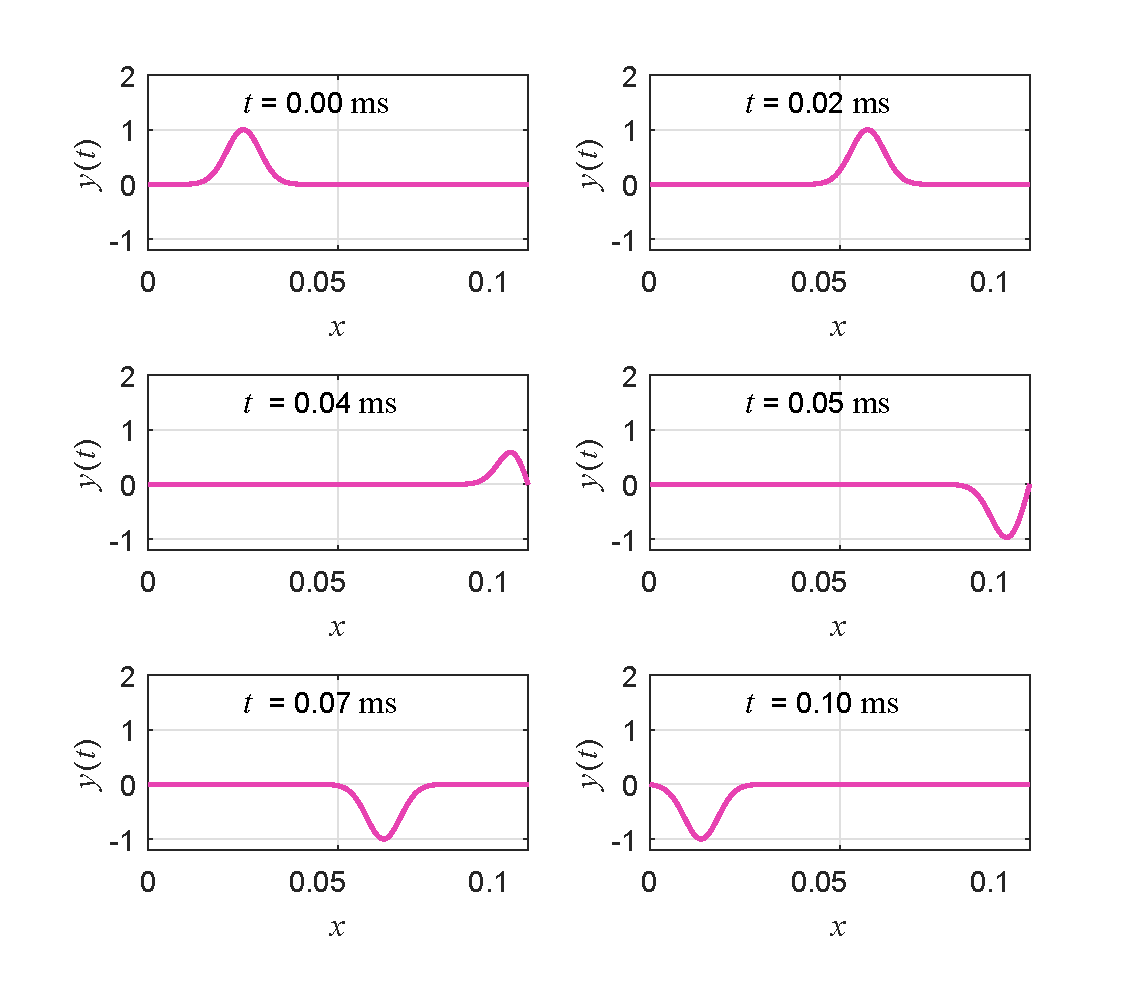
\includegraphics[width=\textwidth]{SchwingendeSaite02.pdf}
    \caption[Gau�sche St�rung auf der eingespannten Saite.]{Eine Gau�sche St�rung
      breitet sich auf der beidseitig eingespannten Saite aus.}
    \label{abb:kontmech_SaiteGausswelle}
  \end{figure}

  \begin{figure}
  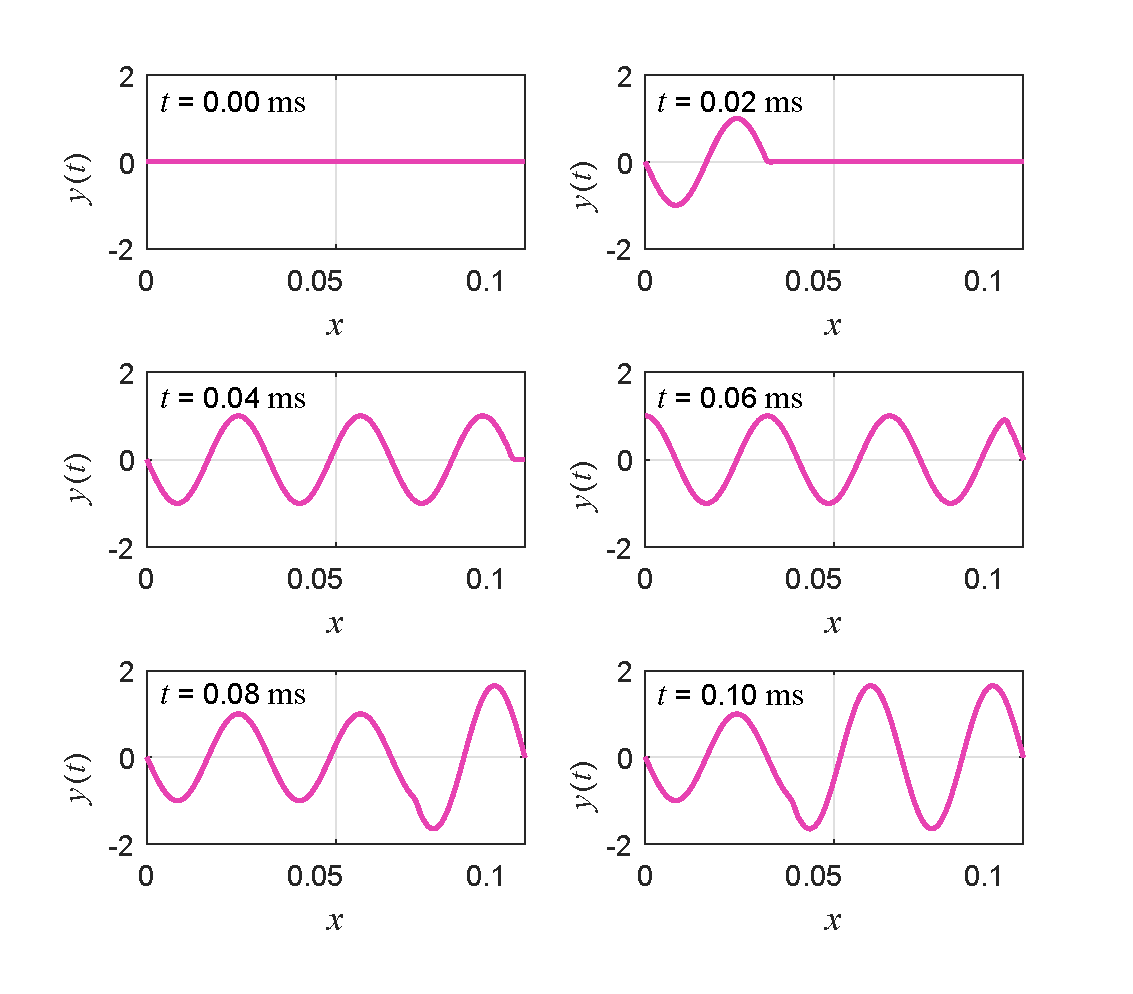
\includegraphics[width=\textwidth]{SchwingendeSaite03.pdf}
  \caption[Angeregte Welle auf der eingespannten Saite.]{Eine Welle wird
    am linken Rand der eingespannten Saite angeregt und am rechten
    Rand reflektiert.}
    \label{abb:kontmech_SaiteAngeregteWelle}
  \end{figure}

\item Im zweiten Fall wird die Anfangsbedingung so gesetzt, dass
  $y(x_i,t=0) = y(x_i,t=\Delta t) = 0$. Einzig der Wert an linken Rand,
  f�r den bisher immer $y(x=0,t_l)= 0$ galt, erh�lt jetzt eine periodische
  Funktion in der Zeit der Form
  \begin{equation*}
    y(x=0,t_l) = \sin \left (\frac{10\,\pi}{T_\mathrm{max}}\, t_l \right ) \;,
  \end{equation*}
  worin $T_\mathrm{max}$ die Ausbreitungszeit �ber die L�nge der Saite ist, \dh die Saite wird mit
	einer Frequenz $5/T_\mathrm{max}$ periodisch am linken Rand angeregt.
	Damit ergibt sich die L�sung aus \figref{kontmech_SaiteAngeregteWelle},
  die eine Welle darstellt, die sich vom linken Rand ausbreitet. Sobald
  sie am rechten Rand ankommt und reflektiert wird, �berlagern sich die
  einlaufende und reflektierte Welle.
  
\end{enumerate}


\end{sol} 
\textcolor{blue} {$\rightarrow$ zur} \probref{kontmech_WelleSaite}.\\
\noindent\rule[1ex]{\textwidth}{0.5pt}  \newpage  \clearpage

%-----------------------------------------------------------------------------------------------------------


\begin{sol}{prob:kontmech_AchterbahnKont}\label{lsg:kontmech_AchterbahnKont} %�bung18
\textbf{Achterbahn-Bewegungsgleichungen im kontinuierlichen Ansatz}\\ \\

Wir starten mit dem Potential nach \eqref{eq:bew_ABdiskret02} aus der
\hyperref[lsg:bew_achterbahn_diskret]{L�sung} zu
\probref{bew_achterbahn_diskret}
\begin{equation*}
  U\lk \{x_i\},\{z_i\}\rk = m\,g\,\sum_{i=1}^{N}z_i + \frac{1}{2}\,k\sum_{i=1}^{N-1}\lk \sqrt{\lk x_{i+1}-x_i\rk^2 + \lk z_{i+1}-z_i\rk^2 }- s_0\rk^2
\end{equation*}
und der kinetischen Energie nach \eqref{eq:bew_ABdiskret02}
\begin{equation}
  T\lk\{\dot{x}_i\},\{\dot{z}_i\}\rk = \frac{1}{2}\,m\sum_{i=1}^{N}\lk \dot{x}_i{}^2 + \dot{z}_i{}^2\rk\,.
  \label{eq:kontmech_AchterbahnGeschw}
\end{equation}
Zun�chst setzen wir hier direkt die Beziehung $z_i=h(x_i)$ ein, um auf die
generalisierte Koordinaten $x_i$ �berzugehen. Dann wird aus den Termen
\begin{equation}
  U\lk \{x_i\}\rk = m\,g\,\sum_{i=1}^{N} h(x_i) + \frac{1}{2}\,k\sum_{i=1}^{N-1}\lk \sqrt{\lk x_{i+1}-x_i\rk^2 + \lk h(x_{i+1})-h(x_i)\rk^2 }- s_0\rk^2
\end{equation}
und der kinetischen Energie nach \eqref{eq:bew_ABdiskret02}
\begin{equation}
  T\lk\{\dot{x}_i\},\{\dot{z}_i\}\rk = \frac{1}{2}\,m\sum_{i=1}^{N}\lk \dot{x}_i{}^2 + \dot{h}(x_i){}^2\rk = \frac{1}{2}\,m\sum_{i=1}^{N}\lk  1 + h'(x_i){}^2 \rk \dot{x}_i{}^2 \,.  
\end{equation}

Die Materiepunkte des Zuges beschreiben wir durch eine Variable $l$ mit
der Eigenschaft $0\leq l \leq L$, wobei $L$ die L�nge des Zuges im
entspannten Zustand auf einer geraden Strecke sein soll. Die tats�chliche
Lage der Materiepunkte im Inertialsystem zu einem beliebigen Zeitpunkt $t$
stellen wir durch die Orte $x(l,t)$ dar.\footnote{Wir wenden also eine
  Beschreibung in Euler-Koordinaten an. Man beachte, dass die Materiepunkte
  unabh�ngig von der aktuellen Lage oder Dehnung des Zuges sich immer auf den
  entspannten Zug auf einer geraden Strecke beziehen und somit die materiellen
  Koordinate $l$ nur Werte zwischen $0$ und $L$ annimmt. Die tats�chliche
  L�nge des Zuges m�ssen wir im Ortsraum bestimmen. Sie ist zu einem
  festen Zeitpunkt $t$ durch $x(L,t)-x(0,t)$ gegeben und kann Werte gr��er
  oder kleiner als $L$ annehmen.}
Um den Kontinuums-Grenzwert vorzubereiten, stellen wir auf:
\begin{subequations}
  \begin{align}
    x_i &\to x(l,t) \\
    s_0 &= \D l \\
    x_{i+1} - x_i &\to \frac{\partial x}{\partial l} \, s_0 =
                          \frac{\partial x}{\partial l} \, \D l\\
    h(x_{i+1}) - h(x_i) &\to \frac{\partial h}{\partial l} \, s_0 = \frac{\partial h}
                          {\partial x} \frac{\partial x}{\partial l} \,s_0
                          = h'(x) \frac{\partial x}{\partial l} \,\D l\\
    m &= \varrho_L \,s_0 = \varrho_L \,\D l \\
    k &= \frac{\Phi}{s_0}
  \end{align}
\end{subequations}
Darin ist $s_0 = \D l$ der Abstand zwischen zwei Wagen in der Ruhelage und
$\varrho_L$ eine L�ngen-Massendichte. Im �bergang vom diskreten Modell zum 
Kontinuum haben wir dann den Kontinuumsgrenzwert f�r $s_0
\to 0$ und $N \to \infty$ bei konstanter Gesamtmasse $M = \varrho_\text{L}\,L$ des Zuges zu bilden.

Mit diesen Definitionen formen wir zun�chst das Potential um. F�r dieses
finden wir
\begin{subequations}
  \begin{align}
    U\lk \{x_i\}\rk
    &= m\,g\,\sum_{i=1}^{N} h(x_i) + \frac{1}{2}\,k\sum_{i=1}^{N-1} \lk
      \sqrt{\lk x_{i+1}-x_i\rk^2 + \lk h(x_{i+1})-h(x_i) \rk^2 }- s_0\rk^2
      \notag \\
    &=  \varrho_L\,g\,\sum_{i=1}^{N} h(x_i) s_0 + \frac{1}{2}\,k\sum_{i=1}^{N-1} \lk
      \sqrt{\lk \frac{\partial x}{\partial l} s_0 \rk^2 + \lk h'(x)
      \frac{\partial x}{\partial l} \,s_0 \rk^2 }- s_0\rk^2 \notag \\
    &=  \varrho_L\,g\,\sum_{i=1}^{N} h(x_i) s_0 + \frac{1}{2}\,k\sum_{i=1}^{N-1}
      \lk \sqrt{1 + h'(x)^2 }\, \frac{\partial x}{\partial l} \, s_0 - s_0\rk^2
      \notag \\
    &=  \varrho_L\,g\,\sum_{i=1}^{N} h(x_i) s_0 + \frac{1}{2}\,k\sum_{i=1}^{N-1}
      \lk \sqrt{1 + h'(x)^2 }\, \frac{\partial x}{\partial l} \, - 1\rk^2 s_0^2
      \notag \\
    &=  \varrho_L\,g\,\sum_{i=1}^{N} h(x_i) s_0 + \frac{1}{2}\,\Phi\,
      \sum_{i=1}^{N-1} \lk \sqrt{1 + h'(x)^2 }\, \frac{\partial x}{\partial l}
      \, - 1\rk^2 s_0
  \end{align}
  Im Grenzwert $s_0 = \D l \to 0$, $N\to\infty$ erkennen wir darin zweimal das
  Riemann\footnote{Georg Friedrich Bernhard Riemann\indexp{Riemann, Georg Friedrich Bernhard} (1826--1866) war ein deutscher Mathematiker, der trotz seines relativ kurzen Lebens als einer der bedeutendsten Mathematiker gilt. Er arbeitete unter anderem bahnbrechend auf den Gebieten der Analysis, Differentialgeometrie und der mathematischen Physik.}-Integral\footnote{Das Riemann-Integral l�sst sich �ber die anschauliche Vorstellung des Integrals als Fl�cheninhalt zwischen der $x$-Achse und dem Graphen einer Funktion definieren. Die zugrundeliegende Idee besteht darin, den gesuchten Fl�cheninhalt mit Hilfe des leicht zu berechnenden Fl�cheninhalts von Rechtecken anzun�hern, \zb von von sogenannten "`Obersummen"' und "`Untersummen"' von Rechtecken, die so gebildet werden, dass der Funktionsgraph zwischen diesen liegt. Indem man  die Anzahl der Rechtecke gegen $\infty$ gehen l�sst, erh�lt man eine immer genauere Approximation des Fl�cheninhalts zwischen dem Funktionsgraphen und der $x$-Achse \cite{Arens2008}.}, was uns f�r einen Zug der L�nge $L$ auf
  \begin{equation}
    U\lk x , \frac{\partial x}{\partial l}\rk =
    \int_{0}^{L} \left \{ \varrho_L\,g\, h(x(l)) + \frac{1}{2}\,\Phi\,
      \lk \sqrt{1 + h'(x(l))^2}\, \frac{\partial x(l)}{\partial l} \, - 1\rk^2
      \right \} \, \D l
    \end{equation}
    f�hrt.
\end{subequations}
Analog finden wir im selben Grenzwert f�r die kinetische Energie
\begin{align}
  T\lk x , \frac{\partial x}{\partial t} \rk
  &= \frac{1}{2}\,m\sum_{i=1}^{N}\lk  1 + h'(x_i){}^2 \rk \dot{x}_i{}^2
  = \frac{1}{2}\,\varrho_L \sum_{i=1}^{N}\lk  1 + h'(x_i){}^2 \rk \dot{x}_i{}^2
  \, s_0 \notag \\
  &= \int_{0}^{L} \frac{1}{2}\,\varrho_L \lk  1 + h'(x(l)){}^2 \rk
    \lk \frac{\partial x}{\partial t} \rk^2 \, \D l \; .
\end{align}
Zusammengef�gt ergibt sich die Lagrange-Funktion
\begin{subequations}
  \begin{equation}
    \mathcal{L} \lk x , \frac{\partial x}{\partial t} , \frac{\partial x}{\partial l} \rk
     = \int_{0}^{L} L \lk x , \frac{\partial x}{\partial t} , \frac{\partial x}{\partial l} \rk \, \D l
  \end{equation}
  mit der Lagrange-Dichte
  \begin{multline}
    L \lk x , \frac{\partial x}{\partial t} , \frac{\partial x}{\partial l} \rk
    = \frac{1}{2}\,\varrho_L \lk  1 + h'(x(l)){}^2 \rk \lk \frac{\partial x}
    {\partial t} \rk^2 \\
    - \varrho_L\,g\, h(x(l)) - \frac{1}{2}\,\Phi\, \lk \sqrt{1 + h'(x(l))^2}
    \, \frac{\partial x(l)}{\partial l} \, - 1\rk^2 \,. \label{eq:kontmech_AchterbahnKont07}
  \end{multline}
\end{subequations}

Wir vergleichen \eqref{eq:kontmech_AchterbahnKont07} mit der
Lagrange-Funktion $\mathcal{L}$ aus \kap{bew_lagrange_formalism} f�r
Massepunkte. Offensichtlich hat im Kontinuumsfall die Lagrange-Dichte
noch eine zus�tzliche unabh�ngige Variable $x' = \partial x / \partial l$, die
wir bereits bei der schwingenden Saite (Beispiel
\ref{bsp:kontmech_schwingendeSaite}) kennen gelernt und ber�cksichtigt hatten. 
Im Unterschied zur schwingenden Saite h�ngt hier nun die Lagrange-Dichte
nicht nur von $\partial x/\partial l$ und $\partial x/\partial t$ ab, sondern
auch noch explizit von $x$. Dies l�sst sich jedoch leicht ber�cksichtigen und 
stellt kein Problem f�r die Variationsrechnung\footnote{Zur Erinnerung: In der
  Variationsrechnung werden die Positionen $x(l)$, die Geschwindigkeiten
  $\dot{x}(l)=\partial x/\partial t$ und die Dehnung $x'(l)=\partial x/
  \partial l$ variiert, wobei die Gesamtl�nge $L$ und die Gesamtzeit der
  Bewegung $T$ konstant bleibt.} dar, mit der wir die Bewegungsgleichung
ableiten wollen. Wir stellen das Wirkungsfunktional
\begin{subequations}
  \allowdisplaybreaks
  \begin{equation}
    S =  \int \D t\, \int_{0}^{L} \D l \, L \lk x , \frac{\partial x}
    {\partial l} , \frac{\partial x}{\partial t} \rk  = \int \D t\, \int_{0}^{L} \D l \, L \lk x , \dot{x}, x' \rk 
  \end{equation}
  auf und f�hren dessen Variation ein,
  \begin{align}
    \delta S &= \int_0^T \D t\, \int_{0}^{L} \D l \, \left \{ L \lk x
               + \delta x ,
               \frac{\partial x}{\partial l} + \frac{\partial \delta x}
               {\partial l},
               \frac{\partial x}{\partial t} + \frac{\partial \delta x}
               {\partial t}
               \rk
               - L \lk x , \frac{\partial x}{\partial l} , \frac{\partial x}
               {\partial t}\rk \right \} \notag \\
             &\overset{\text{Linearisierung}}{\approx}
               \int_0^T \D t\, \int_{0}^{L} \D l \, \left \{
               L \lk x, \frac{\partial x}{\partial l}, \frac{\partial x}
               {\partial t} \rk
               + \frac{\partial L}{\partial x} \, \delta x
               + \frac{\partial L}{\partial \frac{\partial x}{\partial l}}
               \frac{\partial \delta x}{\partial l}
               + \frac{\partial L}{\partial \frac{\partial x}{\partial t}}
               \frac{\partial \delta x}{\partial t}
               - L \lk x , \frac{\partial x}{\partial l} , \frac{\partial x}
               {\partial t}\rk \right \} \notag \\
             &= \int_0^T \D t\, \int_{0}^{L} \D l \, \left \{
               \frac{\partial{L}}
               {\partial x}\,\delta x + \frac{\partial L}{\partial
               \frac{\partial x}{\partial l}} \,  \frac{\partial \delta x}
               {\partial l} + \frac{\partial L}{\partial
               \frac{\partial x}{\partial t}} \,  \frac{\partial \delta x}
               {\partial t} \right \} \notag \\
             &\underset{\text{zweiter Term}}{\overset{\text{part. Int.}}{=}}
               \underbrace{\lek \frac{\partial L}{\partial\frac{\partial x}
               {\partial l}}\, \delta x \rek_0^L}_{=0}
               + \int_0^T \D t\, \int_{0}^{L} \D l \, \left \{
               \frac{\partial{L}}{\partial x}\,\delta x
               - \lk \frac{\partial}{\partial l} \frac{\partial L}
               {\partial\frac{\partial x}{\partial l}} \rk \delta x
               + \frac{\partial L}{\partial \frac{\partial x}{\partial t}}
               \,  \frac{\partial \delta x}{\partial t} \right \} \notag \\
             &\underset{\text{dritter Term}}{\overset{\text{part. Int.}}{=}}
               \underbrace{\lek \frac{\partial L}{\partial\frac{\partial x}
               {\partial t}}\, \delta x \rek_0^T}_{=0}
               + \int_0^T \D t\, \int_{0}^{L} \D l \, \left \{
               \frac{\partial{L}}{\partial x}\,\delta x
               - \lk \frac{\partial}{\partial l} \frac{\partial L}
               {\partial\frac{\partial x}{\partial l}} \rk \delta x
               - \lk \frac{\partial}{\partial t} \frac{\partial L}
               {\partial \frac{\partial x}{\partial t}} \rk \delta x
               \right \} \notag \\
             &= \int_0^T \D t\, \int_{0}^{L} \D l \, \left \{
               \frac{\partial{L}}{\partial x}
               - \frac{\partial}{\partial l} \frac{\partial L}{\partial
               \frac{\partial x}{\partial l}}
               - \frac{\partial}{\partial t} \frac{\partial L}{\partial
               \frac{\partial x}{\partial t}}
               \right \}  \, \delta x \; .
  \end{align}
\end{subequations}
Die Randterme liefern in der partiellen Integration keinen Beitrag, da die
Variation $\delta x$ definitionsgem�� am Rand verschwindet. Die sie aber
ansonsten beliebig ist, lesen wir die notwendige Bedingung
\begin{equation}
  \frac{\partial{L}}{\partial x}
  - \frac{\partial}{\partial t} \frac{\partial L}{\partial
    \frac{\partial x}{\partial t}}
	- \frac{\partial}{\partial l} \frac{\partial L}{\partial
    \frac{\partial x}{\partial l}}=
  \frac{\partial{L}}{\partial x}
  - \frac{\partial}{\partial t} \frac{\partial L}{\partial \dot{x}} 
  - \frac{\partial}{\partial l} \frac{\partial L}{\partial x'} =0
  \label{eq:kontmech_AchterbahnLagrangeDGL}
\end{equation}         
ab. 

Zum Aufstellen der Bewegungsgleichungen m�ssen wir die entsprechenden
Ableitungen bilden. Diese sind:
\begin{subequations}
  \allowdisplaybreaks
  \begin{align}
    \frac{\partial{L}}{\partial x} &= \varrho_L h'(x)h''\frac{\partial L}{\partial\frac{\partial x}{\partial l}} - \varrho_L g h'(x)
                                     - \Phi \lk \sqrt{1 + h'(x)^2}\, \frac{\partial x}{\partial l} - 1 \rk \frac{h'(x)h''(x)} {\sqrt{1 + h'(x)^2}} \,\frac{\partial x}
                                     {\partial l} \, \notag \\
                                   &= \varrho_L h'(x)h''(x) \lk \frac{\partial x}{\partial t} \rk^2 - \varrho_L g h'(x) -\Phi\, h'(x)h''(x) \lk \frac{\partial x}{\partial l} \rk^2 + \Phi\, \frac{h'(x)h''(x)}{\sqrt{1 + h'(x)^2}}\,\frac{\partial x}{\partial l} \\
    \frac{\partial{L}}{\partial \frac{\partial x}{\partial l}} &=- \Phi\, \lk \sqrt{1 + h'(x)^2}\, \frac{\partial x}{\partial l} \,
                                                                 - 1 \rk \sqrt{1 + h'(x)^2} =- \Phi\,\lk \lk \sqrt{1 + h'(x)^2} \rk\, \frac{\partial x}{\partial l} - \sqrt{1 + h'(x)^2} \rk  \\
    \frac{\partial}{\partial l}\frac{\partial L}{\partial\frac{\partial x}{\partial l}} &= - 2 \Phi\, h'(x)h''(x) \, \lk \frac{\partial x}{\partial l} \rk^2 - \Phi\, \lk 1 + h'(x)^2 \rk \frac{\partial^2 x}{\partial l^2} + \Phi\, \frac{h'(x)h''(x)}{\sqrt{1 + h'(x)^2}} \, \frac{\partial x}{\partial l} \\
    \frac{\partial L}{\partial\frac{\partial x}{\partial t}} &= \varrho_L \lk  1 + h'(x){}^2 \rk \frac{\partial x}{\partial t} \\
    \frac{\partial}{\partial t} \frac{\partial L}{\partial\frac{\partial x}{\partial t}} &= 2 \varrho_L \, h'(x)h''(x) \lk \frac{\partial x}{\partial t} \rk^2 + \varrho_L \lk  1 + h'(x){}^2 \rk \frac{\partial^2 x}{\partial t^2}\,.
  \end{align}
\end{subequations}

Dies fasst man in der Bewegungsgleichung
\eqref{eq:kontmech_AchterbahnLagrangeDGL} zusammen zu
\begin{subequations}
  \begin{multline}
    -\varrho_L h'(x)h''(x) \lk \frac{\partial x}{\partial t} \rk^2
    - \varrho_L g h'(x)
    +\Phi\, h'(x)h''(x) \lk \frac{\partial x}{\partial l} \rk^2 \\
    + \Phi\, \lk 1 + h'(x)^2 \rk \frac{\partial^2 x}{\partial l^2}
    - \varrho_L \lk  1 + h'(x){}^2 \rk \frac{\partial^2 x}{\partial t^2}
    = 0 \; ,
  \end{multline}
  was noch nach
  \begin{equation}
    \frac{\partial^2 x}{\partial t^2} = -\frac{h'(x)h''(x)}{1 + h'(x){}^2}
    \lk \frac{\partial x}{\partial t} \rk^2
    - \frac{g h'(x)}{1 + h'(x){}^2}
    +\frac{\Phi}{\varrho_L}\, \frac{h'(x)h''(x)}{1 + h'(x){}^2} \lk
    \frac{\partial x}{\partial l} \rk^2
    + \frac{\Phi}{\varrho_L}\, \frac{\partial^2 x}{\partial l^2}
    \label{eq:kontmech_DGLkontAchterbahn}
  \end{equation}
  aufgel�st werden kann.


  Man beachte insbesondere, dass f�r einen
  starren Zug, der seine L�nge nicht ver�ndern kann, f�r den also
  \begin{equation*}
    x' = \frac{\partial x}{\partial l} = x'' = \frac{\partial^2 x}{\partial l^2}
    = 0
  \end{equation*}
  gilt, die Bewegungsgleichung \eqref{eq:kontmech_DGLkontAchterbahn}
  die Form
  \begin{equation*}
    \ddot{x} = - \frac{h'(x)h''(x)}{1 + h'(x){}^2}\dot{x}^2
    - \frac{g h'(x)}{1 + h'(x){}^2}
  \end{equation*}
  annimmt, die wir schon aus der \hyperref[lsg:bew_achterbahn]{L�sung}
  zu \probref{bew_achterbahn} (vgl. mit den Gleichungen
  \eqref{eq:bew_Achterbahn03} und \eqref{eq:bew_Achterbahn05}) kennen.
\end{subequations}
  
\end{sol} 
\textcolor{blue} {$\rightarrow$ zur} \probref{kontmech_AchterbahnKont}.\\
\noindent\rule[1ex]{\textwidth}{0.5pt}  \newpage  \clearpage

%-----------------------------------------------------------------------------------------------------------

\begin{sol}{prob:kontmech_AchterbahnZug}\label{lsg:kontmech_AchterbahnZug} %�bung19
\textbf{Elastischer Achterbahnzug auf einer Gau�kurven-Strecke}\\ \\

Analog zum Vorgehen bei der schwingenden Saite in Beispiel
\ref{bsp:kontmech_finiteDiffSaite} diskretisieren wir die Bewegungsgleichung.
F�r die erste und zweite Ableitung von $x$ nach der Zeit schreiben wir
\begin{align*}
  \frac{\partial x}{\partial t}
  &\to \frac{x(l_i,t_{j}) - x(l_i,t_{j-1})}{\Delta t} \; ,\\
  \frac{\partial^2 x}{\partial t^2}
  &\to \frac{x(l_i,t_{j+1}) + x(l_i,t_{j-1}) -2 x(l_{i},t_{j})}{\Delta t^2}
    \; .
\end{align*}
Analog bilden wir f�r die Ableitung nach der materiellen Koordinate $l$
\begin{align*}
  \frac{\partial x}{\partial l}
  &\to \frac{x(l_i,t_j) - x(l_{i-1},t_j)}{\Delta l} \; ,\\
  \frac{\partial^2 x}{\partial l^2}
  &\to \frac{x(l_{i+1},t_j) + x(l_{i-1},t_j) -2 x(l_{i},t_{j})}{\Delta t^2}
    \; .
\end{align*}
Eingesetzt in die Differentialgleichung erh�lt man
\begin{align}
\begin{split}
  \frac{x(l_i,t_{j+1}) + x(l_i,t_{j-1}) -2 x(l_{i},t_{j})}{\Delta t^2}
  = -\frac{h'(x)h''(x)}{1+h'(x)^2} \lk \frac{x(l_i,t_{j}) - x(l_i,t_{j-1})}
  {\Delta t} \rk^2 \\
  - g \frac{h'(x)}{1+h'(x)^2}
  + \frac{\Phi}{\varrho_L} \frac{h'(x)h''(x)}{1+h'(x)^2}
  \lk \frac{x(l_i,t_j) - x(l_{i-1},t_j)}{\Delta l} \rk^2 \\
  + \frac{\Phi}{\varrho_L} \frac{x(l_{i+1},t_j) + x(l_{i-1},t_j)
    -2 x(l_{i},t_{j})}{\Delta t^2} \; .  
\end{split} \label{eq:kontmech_DGLkontAchterbahn02}
\end{align}
Dies f�hrt auf die Iterationsgleichung in der Zeit:
\begin{align}
\begin{split}
  x(l_i,t_{j+1}) = 2 x(l_{i},t_{j}) - x(l_i,t_{j-1}) 
  - \frac{h'(x)h''(x)}{1+h'(x)^2} \lk x(l_i,t_{j}) - x(l_i,t_{j-1}) \rk^2 \\
  - g \frac{h'(x)}{1+h'(x)^2} \Delta t^2
  + \frac{\Phi}{\varrho_L} \frac{h'(x)h''(x)}{1+h'(x)^2} \lk \frac{\Delta t}
  {\Delta l} \rk^2 \lk x(l_i,t_j) - x(l_{i-1},t_j) \rk^2 \\
  + \frac{\Phi}{\varrho_L} \lk \frac{\Delta t}
  {\Delta l} \rk^2 \lk x(l_{i+1},t_j) + x(l_{i-1},t_j)
  -2 x(l_{i},t_{j}) \rk
\end{split} \label{eq:kontmech_DGLkontAchterbahn03}
\end{align}
Eine numerische L�sung dieser Gleichung mithilfe der \matlab{}-Datei
\mlkontmechref{AchterbahnKont.m} ist in
\figref{kontmech_AchterbahnKont} dargestellt. Der Zug startet
in diesem Programm zur Zeit $t=0$ weit weg von der Gau�kurvenstrecke und
f�hrt auf diese zu. 
\begin{figure}
  \centering
  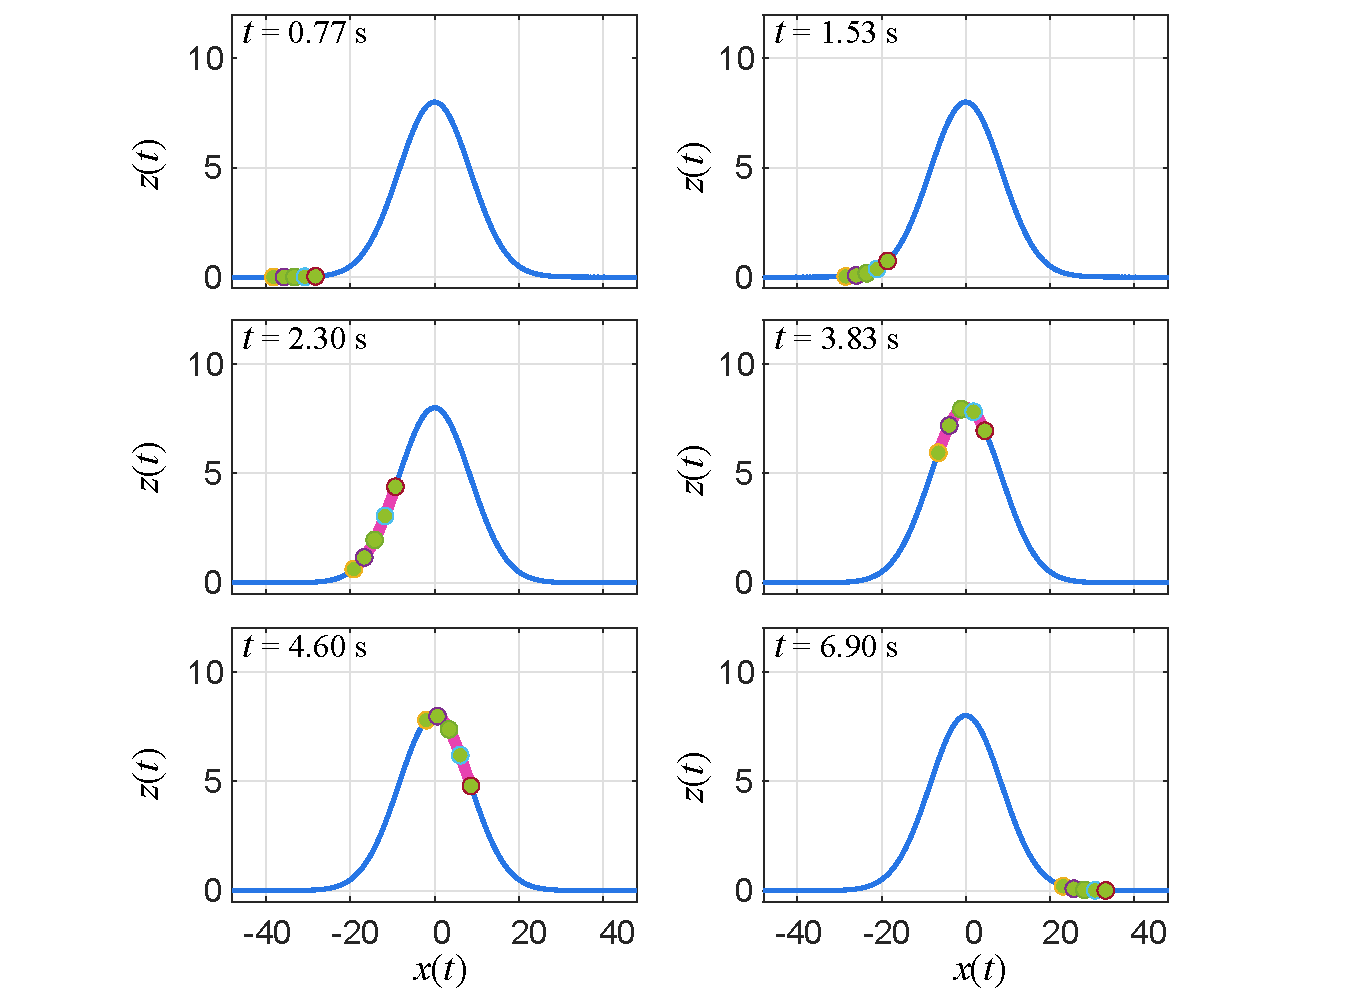
\includegraphics[width=\textwidth]{AchterbahnKont.pdf}
  \caption[Elastischer Achterbahnzug auf der Gau�kurvenstrecke.]
  {Elastischer Achterbahnzug zu verschiedenen Zeitpunkten auf der
    Gau�kurvenstrecke. Die gr�nen Punkte entsprechen materiellen Koordinaten
    in �quidistanten Abst�nden.}
  \label{abb:kontmech_AchterbahnKont}
\end{figure}
In der Berechnung des diskreten Systems eines Zuges aus Wagen, die mit
Federn gekoppelt sind, in der \hyperref[lsg:bew_achterbahn_diskret]{L�sung} zu
\probref{bew_achterbahn_diskret} hat sich bereits gezeigt, dass der Abstand
zwischen den ersten beiden Wagen zun�chst sinkt, wenn der erste Wagen in
die Steigung der Gau�kurvenstrecke f�hrt, und anschlie�end steigt, wenn die
Feder gegen die Bewegung dr�ckt und immer weitere Teile des Zuges gegen
die Gravitation ank�mpfen m�ssen. Dies ist von einer Schwingung durch
die Federn �berlagert. In \figref{kontmech_KreisRohrGeschwindigkeit} ist
etwas �hnliches zu erkennen. Die gr�nen Punkte markieren Punkte mit
konstantem Abstand der materiellen Koordinaten. F�r einen ruhenden, entspannten
Zug sind auch ihre r�umlichen Abst�nde konstant. W�hrend dies kurz vor dem
Erreichen der Gau�kurvenstrecke noch der Fall ist, sieht man wie zu $t=
\SI{1.53}{\second}$ der Abstand zwischen den ersten beiden Wagen steigt. Dies
verst�rkt sich f�r alle Wagen zur Zeit $t=\SI{2.30}{\second}$.

Um die Spitze des Berges herum verdichten sich die Punkte, nach deren
�berwinden steigen die Abst�nde wieder. Auch das hat sich im diskreten Modell
so gezeigt. Mit zunehmender Beschleunigung der hinteren Zugteile, w�hrend der
vordere bereits wieder auf flacheren Streckenteilen unterwegs ist, verk�rzen
sich die Abst�nde nach vorne. Nach �berwinden des Gau�-Berges finden noch
Schwingungsbewegungen des elastischen Zuges statt. Das hei�t, der Zug kehrt
nicht zu seiner reinen Schwerpunktsbewegung zur�ck, die er vor der Gau�kurve
hatte. Ein Teil der Energie wurde in die Relativbewegung der einzelnen
Zugteile gegeneinander transferiert. Diesen Effekt konnte man bereits
im diskreten Modell sehen (vgl.\ \hyperref[lsg:bew_achterbahn_diskret]{L�sung}
zu \probref{bew_achterbahn_diskret}). In einem realen Zug w�rden nat�rlich
sowohl die Relativ- als auch die Schwerpunktsbewegung ged�mpft werden, sodass der
Zug am Ende wieder die urspr�ngliche, entspannte Form annehmen w�rde, aber
auch langsamer w�re als am Beginn der Kurve.

\end{sol} 
\textcolor{blue} {$\rightarrow$ zur} \probref{kontmech_AchterbahnZug}.\\
\noindent\rule[1ex]{\textwidth}{0.5pt}  \newpage  \clearpage

%-----------------------------------------------------------------------------------------------------------

\begin{sol}{prob:kontmech_AchterbahnBeschleunigungen}\label{lsg:kontmech_AchterbahnBeschleunigungen} %�bung20
\textbf{Normalbeschleunigung eines Fahrgastes im Achterbahnzug}\\ \\

Jeder Fahrgast sp�rt in jedem Fall seine Gewichtskraft, die zu einer
Fallbeschleunigung $-g\veceZ$ f�hrt. Dar�ber hinaus folgt er der
Bewegung des Wagens und sp�rt die Radialbeschleunigung der nicht-geradlinigen
Bewegung. Die $x$-Komponente kann prinzipiell aus der Bewegungsgleichung
\eqref{eq:kontmech_DGLkontAchterbahn} extrahiert werden. Wir wollen
hier jedoch die Normalkomponenten mit einer eigenen Betrachtung finden.

Die Radialbeschleunigung hat den Betrag
\begin{equation}
  a_r = \frac{v^2}{r}
\end{equation}
mit der Geschwindigkeit $v$ entlang der Bahn und dem Radius $r$ des Kreises,
der an der Bahn anliegt und deren Kr�mmung im entsprechenden Bahnpunkt
wiedergibt. Die Geschwindigkeit $v$ erhalten wir direkt aus der numerischen
L�sung des Bahnverlaufs.
Um $r$ zu bestimmen, suchen wir erst den Kreis, der an der Bahn anliegt und
dessen Funktion $z(x)$ die Kr�mmung der Bahn richtig wiedergibt, siehe
\figref{kontmech_KreisAnliegend}.

\begin{figure}
  \centering
  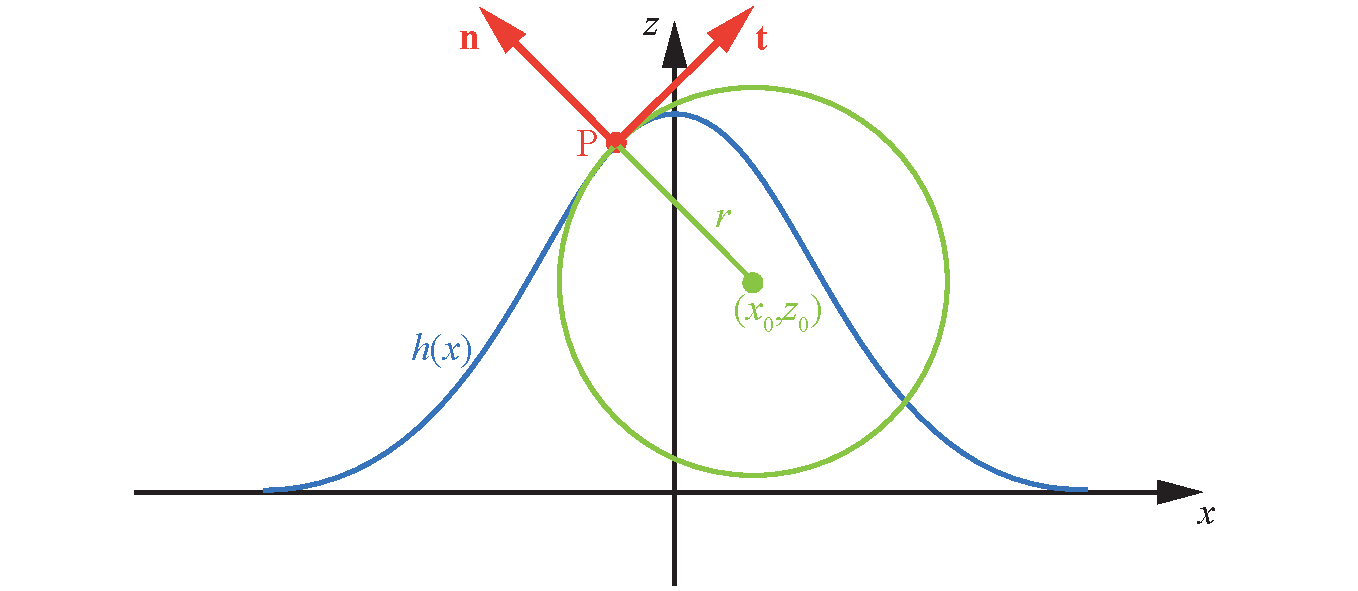
\includegraphics[width=\textwidth]{AchterBahnKreis.pdf}
  \caption[Kreis zur Bestimmung der Radialbeschleunigung.]
  {Kreis, der an die Achterbahnkurve anliegt und die Kr�mmung am Punkt
    P korrekt beschreibt, um daraus die Radialbeschleunigung zu bestimmen.}
  \label{abb:kontmech_KreisAnliegend}
\end{figure}

Zur Berechnung l�sen wir die Kreisgleichung
\begin{subequations}
  \begin{equation}
    (x-x_0)^2 + (z-z_0)^2 = r^2
  \end{equation}
  nach 
  \begin{equation}
    z(x) = \pm \sqrt {r^2 - (x-x_0)^2 }
  \end{equation}
\end{subequations}
auf. Um die richtige Steigung f�r das Anliegen und die richtige Kr�mmung
bestimmen zu k�nnen, ben�tigen wir die erste und die zweite Ableitung. Beide
m�ssen anschlie�end mit der Bahn �bereinstimmen. Die erste Ableitung
f�hrt auf
\begin{subequations}
  \begin{equation}
    \frac{\D z}{\D x} = \mp \frac{x-x_0}{\sqrt {r^2 - (x-x_0)^2 }}
    = - \frac{x-x_0}{z-z_0}
  \end{equation}
  und damit erhalten wir
  \begin{multline}
    \frac{\D^2 z}{\D x^2} = \frac{\D}{\D x} \lk - \frac{x-x_0}{z-z_0} \rk
    = - \frac{x-x_0}{z-z_0} = - \frac{1}{z-z_0} + \frac{x-x_0}{(z-z_0)^2}
    \frac{\D z}{\D x} \\
    = - \frac{1}{z-z_0} - \frac{1}{(z-z_0)} \lk \frac{\D z}{\D x} \rk^2 
    = - \frac{1}{z-z_0} \lk 1 + \lk \frac{\D z}{\D x} \rk^2 \rk
  \end{multline}
\end{subequations}

Damit der Kreis wie gew�nscht an der Kurve anliegt, m�ssen die drei
Gleichungen
\begin{subequations}
  \begin{align}
    z(x) &= \pm \sqrt {r^2 - (x-x_0)^2 } \overset{!}{=} h(x) \\
    \frac{\D z}{\D x} &= - \frac{x-x_0}{z-z_0} \overset{!}{=} h'(x) \\
    \frac{\D^2 z}{\D x} &= - \frac{1}{z-z_0} \lk 1 + \lk \frac{\D z}{\D x}
                          \rk^2 \rk = - \frac{1}{z-z_0} \lk 1 + h'(x)^2
                          \rk \overset{!}{=} h''(x)
  \end{align}
\end{subequations}
erf�llt sein. Die letzte Gleichung l�sst sich zu
\begin{subequations}
  \begin{equation}
   z-z_0 = \frac{1+h'^2}{h''}
 \end{equation}
 aufl�sen, was mit der zweiten auf
  \begin{equation}
   x-x_0 = - \frac{1+h'^2}{h''} h'
 \end{equation}
 f�hrt und schlie�lich mit der ersten zur Bestimmung des Radius nach
 \begin{equation}
   r = \frac{1+h'^2}{h''} \sqrt{1+h'^2}
 \end{equation}
\end{subequations}
herangezogen werden kann.

Mit dem Geschwindigkeitsquadrat nach \eqref{eq:kontmech_AchterbahnGeschw}
\begin{equation}
  v^2 = (1+h'^2) \dot{x}^2
\end{equation}
ergibt sich die Radialbeschleunigung zu
\begin{equation}
  a_r = \frac{h''}{1+h'^2}\sqrt{1+h'^2}\, \dot{x}^2 \; .
\end{equation}
Um ihr eine Richtung zu geben, f�hren wir den normierten Tangentialvektor an
die Achterbahnkurve (siehe \figref{kontmech_KreisAnliegend})
\begin{subequations}
  \begin{equation}
    \vec{t} = \frac{1}{\sqrt{\D x^2 + \D z^2}} \begin{pmatrix} \D x \\
      \D z \end{pmatrix}
    = \frac{1}{\sqrt{(1 + h'(x)^2) \D x^2}} \begin{pmatrix} \D x \\
      h'(x) \D x \end{pmatrix}
    =  \frac{1}{\sqrt{1 + h'(x)^2}} \begin{pmatrix} 1 \\
      h'(x)  \end{pmatrix}
  \end{equation}
  ein und bilden den dazu Normalenvektor, der immer nach au�en zeigt,
  \begin{equation}
    \vec{n} = \frac{1}{\sqrt{1 + h'(x)^2}} \begin{pmatrix} -h'(x) \\
      1 \end{pmatrix} \; .
  \end{equation}
\end{subequations}
Damit lautet die vektorielle Darstellung der Radialbeschleunigung
\begin{equation}
  \vec{a}_r = \frac{h''}{1+h'^2}\sqrt{1+h'^2}\,  \dot{x}^2 \, \vec{n}
  = \frac{h''}{1+h'^2} \dot{x}^2 \begin{pmatrix} -h'(x) \\ 1 \end{pmatrix}
  \; .
\end{equation}
Daraus gewinnen wir die Komponenten
\begin{subequations}
  \begin{align}
    a_{r,x} &= -\frac{h'' h'}{1+h'^2}\, \dot{x}^2 \; , \\
    a_{r,z} &= \frac{h''}{1+h'^2}\, \dot{x}^2 \; .
  \end{align}
\end{subequations}

Zur Vollst�ndigkeit geben wir die Normalkomponenten der Schwerebeschleunigung
\begin{equation}
  g_n = -g\veceZ\cdot \vec{n} = - \frac{g}{\sqrt{1+h'^2}}
\end{equation}
an. Damit lautet die Normalbeschleunigung
\begin{equation}
  a_n = a_r + g_n = \frac{h''}{1+h'^2}\sqrt{1+h'^2}\, \dot{x}^2
  - \frac{g}{\sqrt{1+h'^2}}
\end{equation}
und sie hat die Komponenten
\begin{subequations}
  \begin{align}
    a_{n,x} &= a_x = -\frac{h'' h'}{1+h'^2}\, \dot{x}^2 \; , \\
    a_{n,z} &= \frac{h''}{1+h'^2}\, \dot{x}^2 -g \; .
  \end{align}
\end{subequations}

\begin{figure}
  \centering
  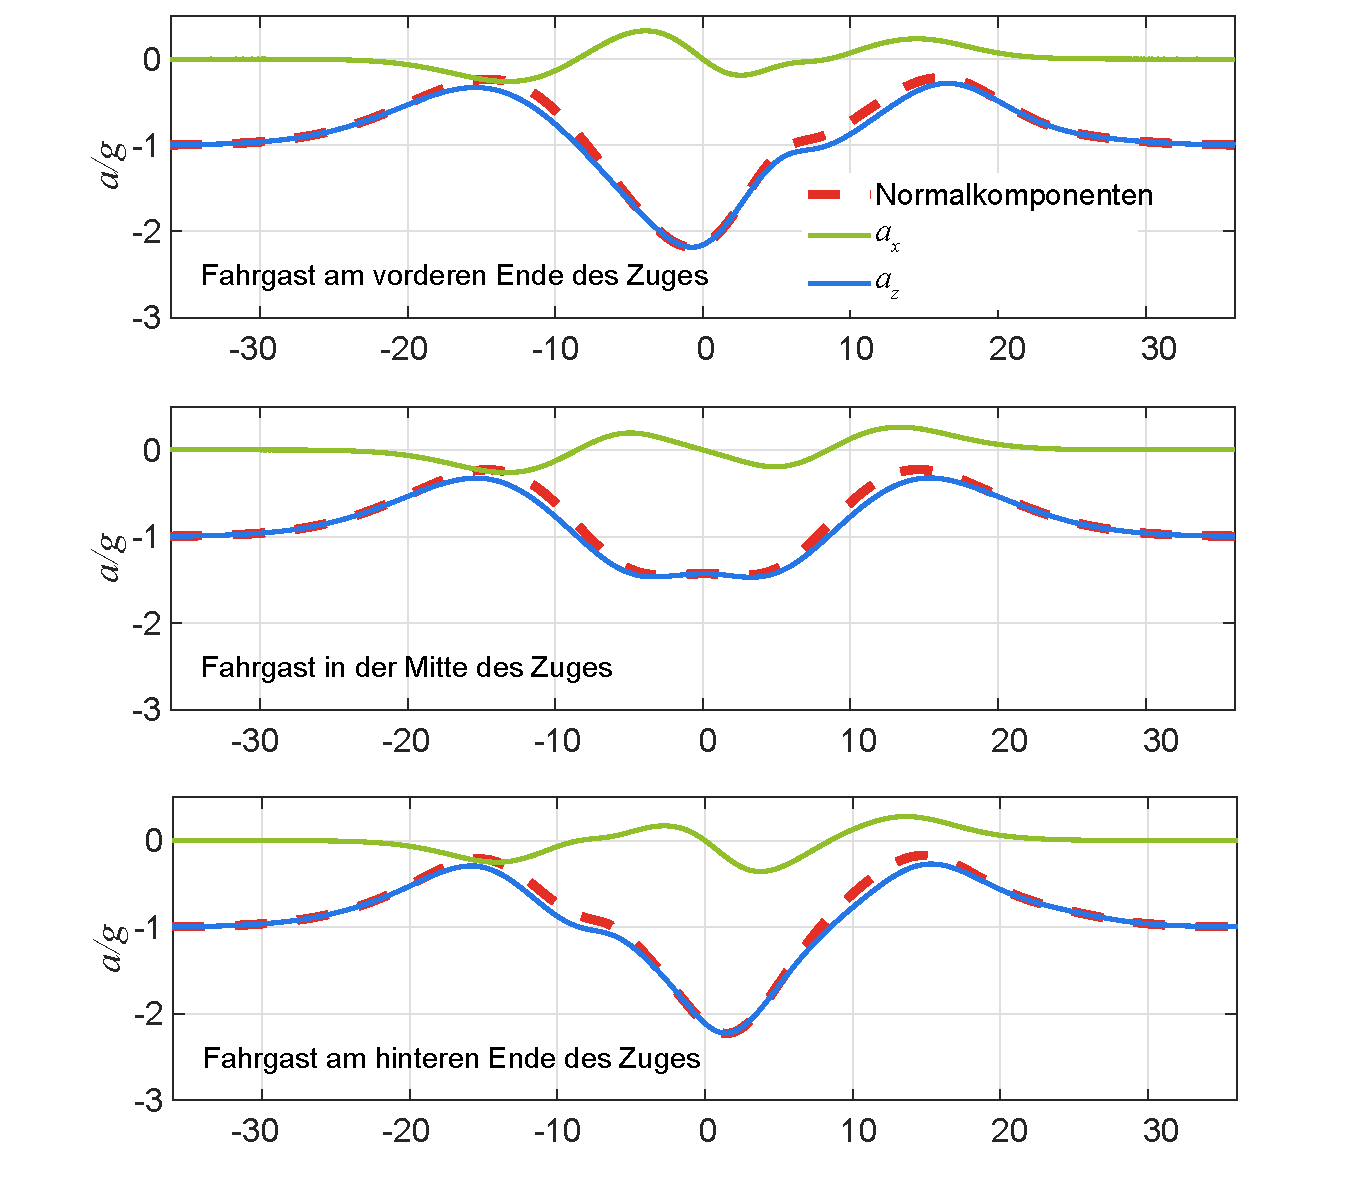
\includegraphics[width=\textwidth]{ABKontNormBeschl.pdf}
  \caption[Normalbeschleunigung auf einen Fahrgast im Achterbahnzug.]{Normalbeschleunigung auf einen Fahrgast im
    Achterbahnzug auf der Gau�kurvenstrecke. Gezeigt sind zus�tzlich die
    $x$- und $z$-Komponenten.}
  \label{abb:kontmech_AchterbahnKontNormalBeschl}
\end{figure}

Ein Beispiel f�r eine L�sung wird im \matlab{}-Programm
\mlkontmechref{AchterbahnKontBeschl.m} vorgestellt.
Die Normalbeschleunigung sowie ihre $x$- und $z$-Komponenten sind in
\figref{kontmech_AchterbahnKontNormalBeschl} f�r den Fall einer
Gau�-Kurve als Achterbahn dargestellt. Im Vergleich mit dem
diskreten Modell, das wir aus der \hyperref[lsg:bew_achterbahn_diskret]{L�sung}
zu \probref{bew_achterbahn_diskret} kennen, f�llt zun�chst auf, dass die
Kr�fte deutlich weniger symmetrisch um den Berg der Achterbahn wirken. Das
liegt daran, dass im elastischen kontinuierlichen Modell deutlich st�rker
Energie in die Schwingungsbewegung eingekoppelt wird, als es bei diskreten
Wagen, die mit wenigen harten Federn verbunden sind, der Fall ist. Dadurch
wirkt die Form der Kraft auch deutlich unruhiger.
Der qualitative Verlauf des diskreten Modells best�tigt sich jedoch. Um
den Berg herum, ist eine deutliche negative (also nach innen bzw. unten
gerichtete) Normalkraft n�tig, um den Fahrgast auf der Bahn zu halten.
W�hrend er sich zwischen Sitz und Sicherheitshaltung bewegt hat der das Gef�hl,
abzuheben (Airtime) und wird dann aus seiner Sicht in die Sicherheitshaltung
gedr�ckt. Ebenfalls wie im diskreten Modell zeigt sich, dass ein Fahrgast im
mittleren Wagen um den Berg herum eine schw�chere Normalkraft erf�hrt als
Fahrg�ste am Rand.

\end{sol} 
\textcolor{blue} {$\rightarrow$ zur} \probref{kontmech_AchterbahnBeschleunigungen}.\\
\noindent\rule[1ex]{\textwidth}{0.5pt}  \newpage  \clearpage

%-----------------------------------------------------------------------------------------------------------

\begin{sol}{prob:kontmech_ElastizitaetTorsion}\label{lsg:kontmech_ElastizitaetTorsion} %�bung21
\textbf{Elastizit�ts-/Torsionsmodul im dreidimensionalen Spannungstensor}\\ \\

Der Spannungstensor eines elastischen, dreidimensionalen K�rpers hat die
Form
\begin{equation}
  \sigma_{ij} = i \lk  \frac{\partial u_i}{\partial p_j} +
  \frac{\partial u_j}{\partial p_i} \rk + \lambda
  \sum_k \frac{\partial u_k}{\partial p_k} \delta_{ij}
  \label{eq:kontmech_SpannungstensorAufg}
\end{equation}
mit
\begin{subequations}
  \begin{align}
    \lambda &= \frac{j}{(1-2j)(1+j)} E \; ,
              \label{eq:kontmech_ElModAufg} \\
    i &= G = \frac{1}{2} \frac{1}{1+j} E \; .
          \label{eq:kontmechTorModAufg}
  \end{align}
\end{subequations}

Aus diesem m�ssen sich Elastizit�ts- und Torsionsmodul erneut gewinnen
lassen.

Ein Fall, in dem sich ausschlie�lich ein Elastizit�tsmodul bemerkbar macht,
entspricht einer Streckung oder Stauchung in Richtung der Kraftwirkung.
Wir ben�tigen also ein Element $\sigma_{ii}$ des Spannungstensors.
Beispielhaft rechnen wir dies f�r das Element $\sigma_{xx}$ durch. Zusammen
mit den Lam\'e-Konstanten \eqref{eq:kontmech_ElModAufg} und
\eqref{eq:kontmechTorModAufg} erhalten wir in der Definition
\eqref{eq:kontmech_SpannungstensorAufg} des Spannungstensors
\begin{multline}
  \sigma_{xx} = 2 i \frac{\partial u_x}{\partial p_x}
  + \lambda \lk \frac{\partial u_x}{\partial p_x} +
  \frac{\partial u_y}{\partial p_y} + \frac{\partial u_z}{\partial p_z} \rk
  = 2 i \frac{\partial u_x}{\partial p_x}
  + \lambda \lk 1-2j \rk \frac{\partial u_x}{\partial p_x} \\
  = 2 \frac{1}{2} \frac{1}{1+j} E \frac{\partial u_x}{\partial p_x}
  + \frac{j}{(1-2j)(1+j)} E \lk 1-2j \rk \frac{\partial u_x}
  {\partial p_x} \\
  = \frac{1 + j}{1+j} E \frac{\partial u_x}{\partial p_x}
  = E \frac{\partial u_x}{\partial p_x}
  = E \frac{\Delta \ell}{\ell}
\end{multline}
Es ergibt sich also genau die Streckung oder Stauchung mit dem
Elastizit�tsmodul.

Eine Scherung entspricht einem tangentialen Angreifen der Kraft, beispielsweise
ist ausschlie�lich die Verschiebung
\begin{equation*}
  \frac{\partial u_y}{\partial p_x}
\end{equation*}
nichtverschwindend, weil die Verschiebung einer Ebene mit konstantem $p_x$ in
Richtung $u_y$ betrachtet wird. Die zugeh�rigen Elemente des Spannungstensors
lauten
\begin{equation}
  \sigma_{xy} = \sigma_{yx} = i \frac{\partial u_y}{\partial p_x}
  = G \frac{\partial u_y}{\partial p_x} \; .
\end{equation}
Daher ist es sehr konsequent, dass das Torsionsmodul direkt im
Spannungstensor als Vorfaktor auftritt.

\end{sol} 
\textcolor{blue} {$\rightarrow$ zur} \probref{kontmech_ElastizitaetTorsion}.\\
\noindent\rule[1ex]{\textwidth}{0.5pt}  \newpage  \clearpage

%-----------------------------------------------------------------------------------------------------------

\begin{sol}{prob:kontmech_BogenSpannung}\label{lsg:kontmech_BogenSpannung} %�bung22
  \textbf{Bogen mit Spannung durch eine Saite}\\ \\

  Um die Schwingungsfrequenz des Bogens zu berechnen, l�sen wir die
  Differentialgleichung
  \begin{equation*}
    \frac{\partial^4 n}{\partial s^2} = 
    \frac{m \omega^2}{E I h} n + \frac{F}{E I h} \; .
  \end{equation*}
  Sie l�sst sich sehr gut mit einem Runge-Kutta-Algorithmus 4. Ordnung
  und fester Schrittweite integrieren. Dazu schreiben wir die
  Differentialgleichung 4. Ordnung in vier Differentialgleichungen 1. Ordnung
  um,
  \begin{align*}
    \frac{\partial n_0}{\partial s} &= n_1 \; , \\
    \frac{\partial n_1}{\partial s} &= n_2 \; , \\
    \frac{\partial n_2}{\partial s} &= n_3 \; , \\
    \frac{\partial n_3}{\partial s} &=
    \frac{m \omega^2}{E I h} n + \frac{F}{E I h} \; .
  \end{align*}
  Als Startwerte f�r die Integration werden $n_0(0) = n_a$, $n_1(0) = n'_a$,
  $n_2(0) = 0$ und $n_3(0) = 0$ verwendet. Die Werte von $n'_a$ und $\omega$
  werden so lange variiert, bis am Ende der Integration bei $s=L$ die
  Randbedingungen $n_2(L) = 0$ und $n_3(L) = 0$ erf�llt sind. Dies
  l�sst sich mit der nichtlinearen Nullstellensuche \texttt{fsolve} aus
  der Optimization Toolbox von \matlab{} automatisiert umsetzen. Ein
  Beispielprogramm ist in der \matlab{}-Datei \mlkontmechref{GespannterBogen.m}
  gegeben.

  Das Beispielprogramm arbeitet mit 2000 Integrationsschritten. Jeweils 10
  Schritte vom Rand wird die Spannkraft der Saite mit
  \begin{equation*}
    F= T_1 \cos(\vartheta)\, \left | \frac{\partial n}{\partial s} \right |
    - 2k\,n\, \sin^2(\vartheta)
  \end{equation*}
  angesetzt. Der Betrag wird eingef�hrt, um sicherzustellen, dass die
  Spannkraft unabh�ngig vom Vorzeichen der gew�hlten Anfangsbedingungen immer
  in dieselbe Richtung zeigt. Die Saite zieht am Bogen. In allen anderen
  Integrationsschritten gilt $F=0$. F�r die Bestimmung der Eigenfrequenz des
  Bogens ohne spannende Saite wird $F=0$ in allen Integrationsschritten
  angesetzt.
  
  F�r die Parameter aus der Aufgabenstellung ist die Schwingungsfrequenz
  ohne Saite ($f_0$) und f�r die Spannkr�fte von $T_1 = \SI{20}{\newton}$,
  $\SI{50}{\newton}$ und $\SI{100}{\newton}$ in
  \figref{kontmech_GespannterBogen1} gezeigt. Man sieht deutlich, dass bei
  niedrigen Biegungen in der Ruhelage (kleinen Winkeln $\vartheta$) die
  Schwingungsfrequenz kleiner als f�r den Bogen ohne �u�ere Spannung ist.
  F�r gr��eres $\vartheta$ steigt die Frequenz jedoch an und erreicht
  schlie�lich deutlich h�here Werte als $f_0$.

  \begin{figure}
    \centering
    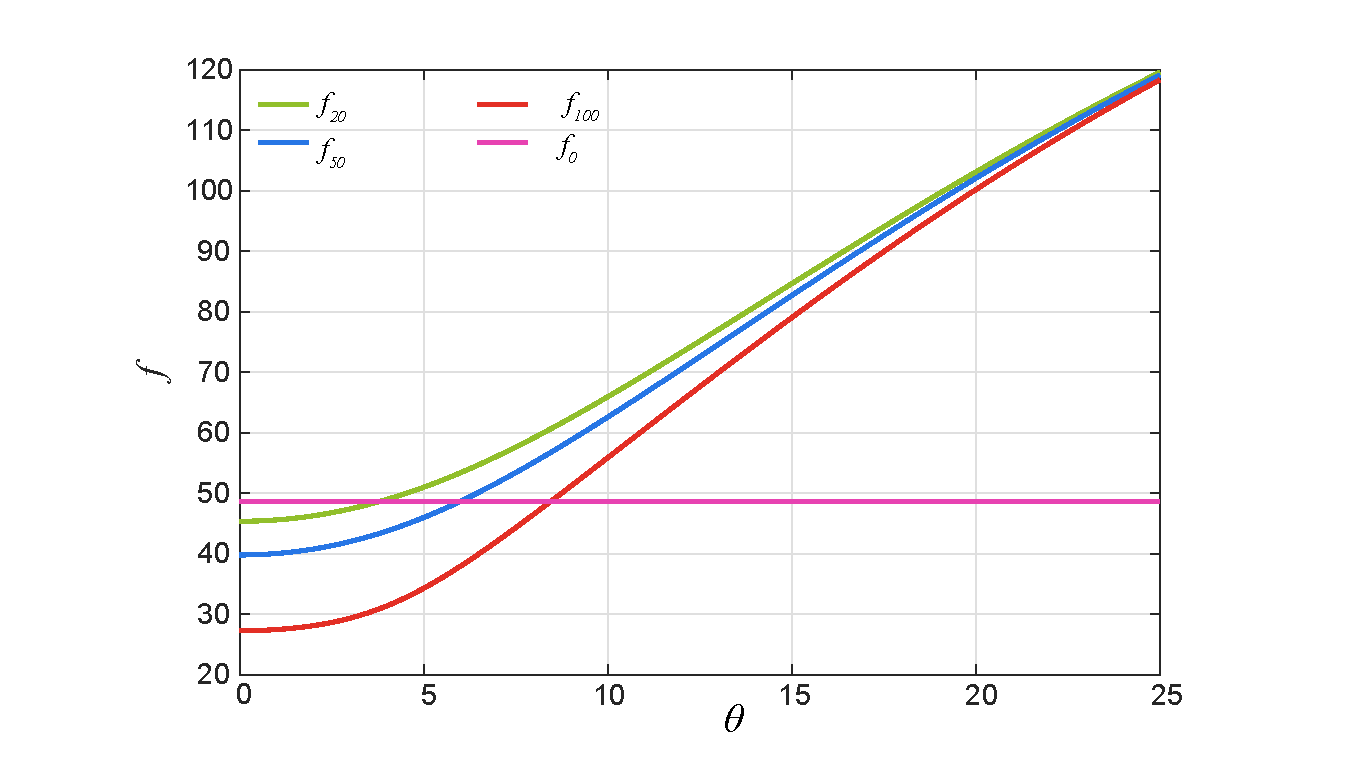
\includegraphics[width=\textwidth]{GespannterBogen1.pdf}
    \caption[Schwingungsfrequenzen eines gespannten Bogens.]
    {Schwingungsfrequenzen eines gespannten Bogens f�r verschiedene
      Winkel $\theta$ der Kr�mmung in der Ruhelage.}
    \label{abb:kontmech_GespannterBogen1}
  \end{figure}

  Der Grund f�r die zwei verschiedenen Verhalten l�sst sich mit den
  verschiedenen Richtungen erkl�ren, in denen die Saite wirkt. F�r einen
  geraden Bogen ($\vartheta = 0$) oder eine schwache Kr�mmung entsteht erst
  durch die Auslenkung der Schwingung eine von der Saite verursachte
  Kraftkomponente senkrecht zur Achse des Bogens, also in Richtung der
  Auslenkung. Diese unterst�tzt die Auslenkung. Der Bogen wirkt dadurch
  weicher und die Schwingungsfrequenz sinkt \cite{Cross2001}. Bei einer
  gr��eren Kr�mmung �berwiegt der Effekt, dass der Bogen durch die Form
  bereits eine Spannkraft hat, die durch die Spannkraft der Saite unterst�tzt
  wird. �hnlich wie in dem Fall, dass parallel an zwei Federn gezogen wird,
  addieren sich die Federkonstanten und der Bogen wird steifer
  \cite{Cross2001}. Die Schwingungsfrequenz steigt folglich.

  Damit l�sst sich auch der Unterschied der Wirkung der gespannten Saite
  auf einen Bogen und einen Schl�ger erkl�ren. Bei einem Schl�ger sind die
  Saiten eintlang der Hauptachsen des Schl�gers gespannt. Sie verursachen
  die Kr�mmung des Schl�gers nicht. Das kommt dem Fall einer sehr geringen
  Kr�mmung $\vartheta \approx 0$ sehr nahe und wie oben beschrieben unterst�tzt
  die Saite damit die Schwingungsbewegung. Sie l�sst den Schl�ger weicher
  wirken. Anders sieht es bei einem Bogen aus. Bei diesem ist die Saite
  typischerweise so gespannt, dass die Kr�mmung des Bogens erst durch sie
  gegeben ist oder die Saite diese verst�rkt. Wir sind also im Fall eines
  gro�en Winkels $\vartheta \gg 0$ und die Saite verst�rkt die R�ckstellkr�ft.
  Sie l�sst den Bogen h�rter wirken als im Fall ohne Saite.
  
  Eine typische Auslenkung und deren erste Ableitung ist f�r den h�chsten
  Winkel $\vartheta = 25^\circ$ im Fall der Federspannung
  $T_1 = \SI{100}{\newton}$ in \figref{kontmech_GespannterBogen2} dargestellt.
  Die zweite und dritte Ableitung sind in \figref{kontmech_GespannterBogen3}
  aufgetragen. Den Einfluss der Seite kann an an den beiden Stellen, an denen
  sie angreift, gut erkennen.

  \begin{figure}
    \centering
    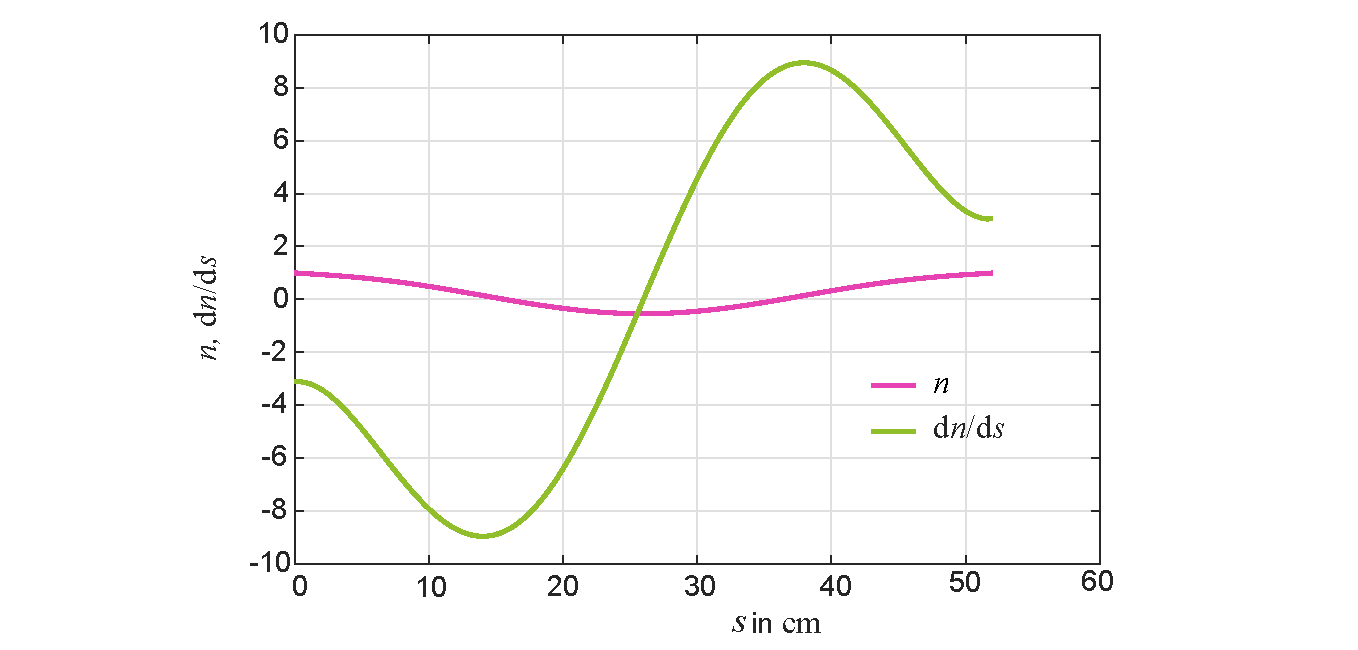
\includegraphics[width=\textwidth]{GespannterBogen2.pdf}
    \caption[Auslenkung der Schwingung eines gespannten Bogens.]
    {Auslenkung der Schwingung eines gespannten Bogens f�r den
      Winkel $\theta = 25^\circ$ und die Spannkraft $T_1 = \SI{100}{\newton}$.}
    \label{abb:kontmech_GespannterBogen2}
  \end{figure}

  \begin{figure}
    \centering
    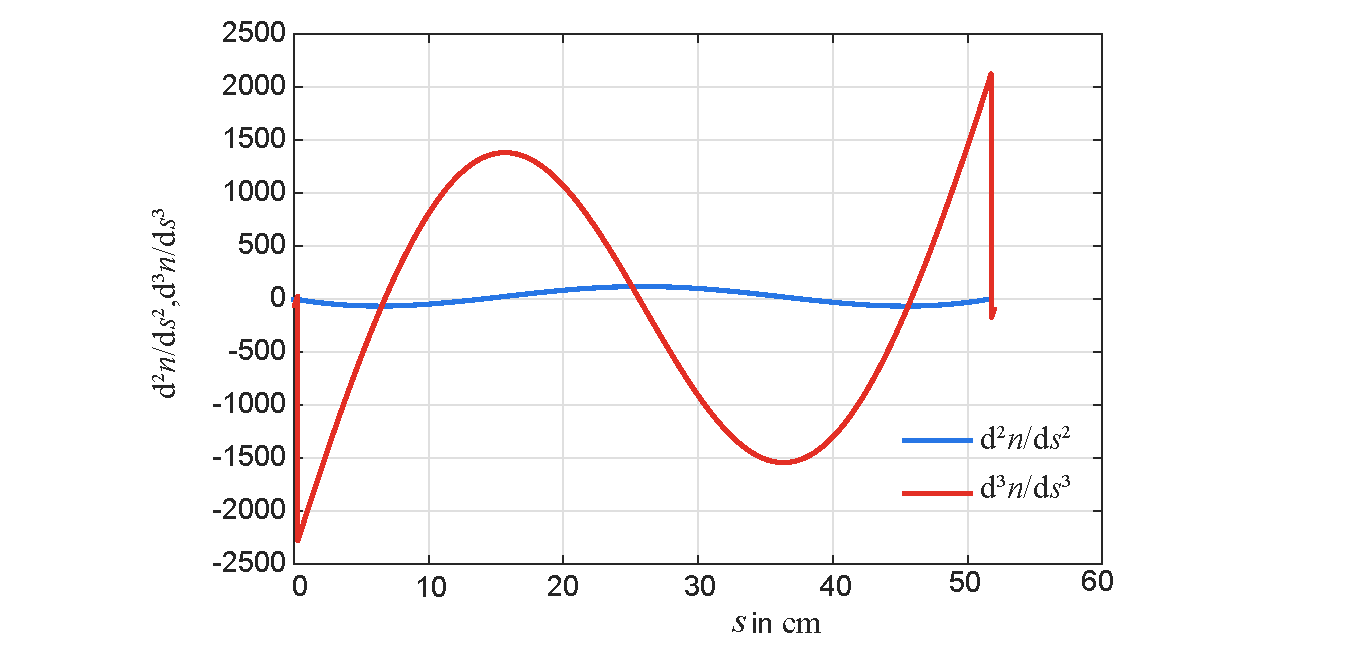
\includegraphics[width=\textwidth]{GespannterBogen3.pdf}
    \caption[Zweite und dritte Ableitung der Schwingung eines gespannten Bogens.]
    {Zweite und dritte Ableitung der Auslenkung der Schwingung eines gespannten
      Bogens f�r den Winkel $\theta = 25^\circ$ und die Spannkraft
      $T_1 = \SI{100}{\newton}$.}
    \label{abb:kontmech_GespannterBogen3}
  \end{figure}
\end{sol} 
\textcolor{blue} {$\rightarrow$ zur} \probref{kontmech_BogenSpannung}.\\
\noindent\rule[1ex]{\textwidth}{0.5pt}  \newpage  \clearpage

%-----------------------------------------------------------------------------------------------------------

\begin{sol}{prob:kontmech_Chladni}\label{lsg:kontmech_Chladni} %�bung23
\textbf{Chladnische Klangfiguren}\\ \\

Die schwingende Scheibe stellt einen zweidimensionalen elastischen K�rper
dar. F�r die Berechnung legen wir die Koordinaten der Scheibe in die
$x$-$y$-Ebene und beschreiben die Auslenkung aus der Ruhelage durch eine
Verschiebung $u_z(x,y,t)$ in $z$-Richtung. Die Differentialgleichung f�r die
elastische Scheibe l�sst sich entsprechend zu
\begin{equation}
  \varrho \frac{\partial^2 z(x,y,t)}{\partial t^2} = i \lk
  \frac{\partial^2 z(x,y,t)}{\partial x^2}
  + \frac{\partial^2 z(x,y,t)}{\partial y^2} \rk
  \label{eq:kontmech_schwingendeScheibe}
\end{equation}
aufstellen. Die Randbedingung bestehen darin, dass auf dem Kreisring, der
die Scheibe begrenzt, die Auslenkung verschwindet, $z=0$.

Ein solches Problem l�sst sich mit der Partial Differential Equation Toolbox
von \matlab{} recht einfach l�sen, indem man die Differentialgleichung
aufstellt und dann mittels des \matlab{}-Kommandos \mlcmd{solvepdeeig}
l�st. Ein Beispiel f�r eine runde Gummischeibe ist in der \matlab{}-Datei
\mlkontmechref{Chladni01.m} gegeben. In \figref{kontmech_ChladniKreis} sind
die L�sungen f�r die ersten sechs Eigenwerte gezeigt.


Vollkommen analog l�sst sich das Problem f�r eine andere Form der Scheibe
l�sen. Einzig die Form des Rands �ndert sich und die Randbedingungen m�ssen
daran angepasst werden. In Abbildung \figref{kontmech_ChladniQuadrat}
ist dies f�r eine quadratische Platte gezeigt, die wiederum nur ein
Spezialfall der rechteckigen Platte aus \figref{kontmech_ChladniRechteck}
ist. Die zugeh�rigen \matlab{}-Dateien sind \mlkontmechref{Chladni02.m}
und \mlkontmechref{Chladni03.m}.

\newpage
\begin{figure}
  \centering
  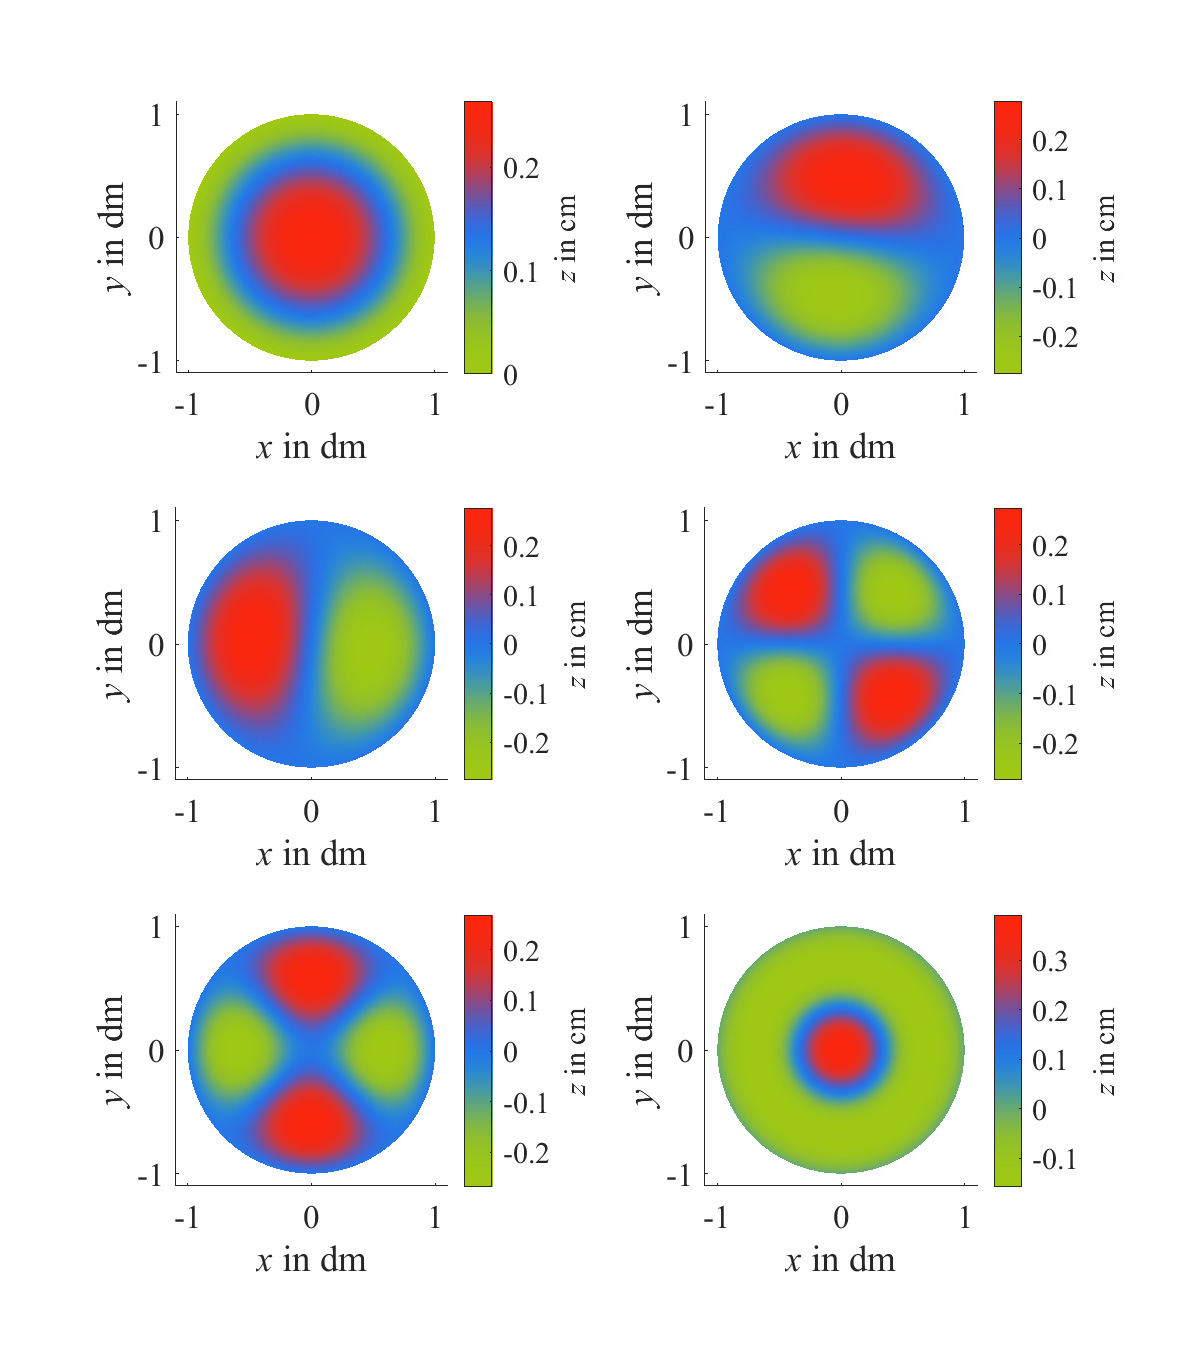
\includegraphics[width=\textwidth]{Chladni_Kreis.pdf}
  \caption[Chladnische Klangfiguren f�r eine kreisf�rmige Fl�che.]
  {Chladnische Klangfiguren f�r eine kreisf�rmige Fl�che. Dargestellt sind die
    numerischen L�sungen f�r die ersten sechs Eigenschwingungen der
    elastischen Fl�che.}
  \label{abb:kontmech_ChladniKreis}
\end{figure}

\newpage
\begin{figure}
  \centering
  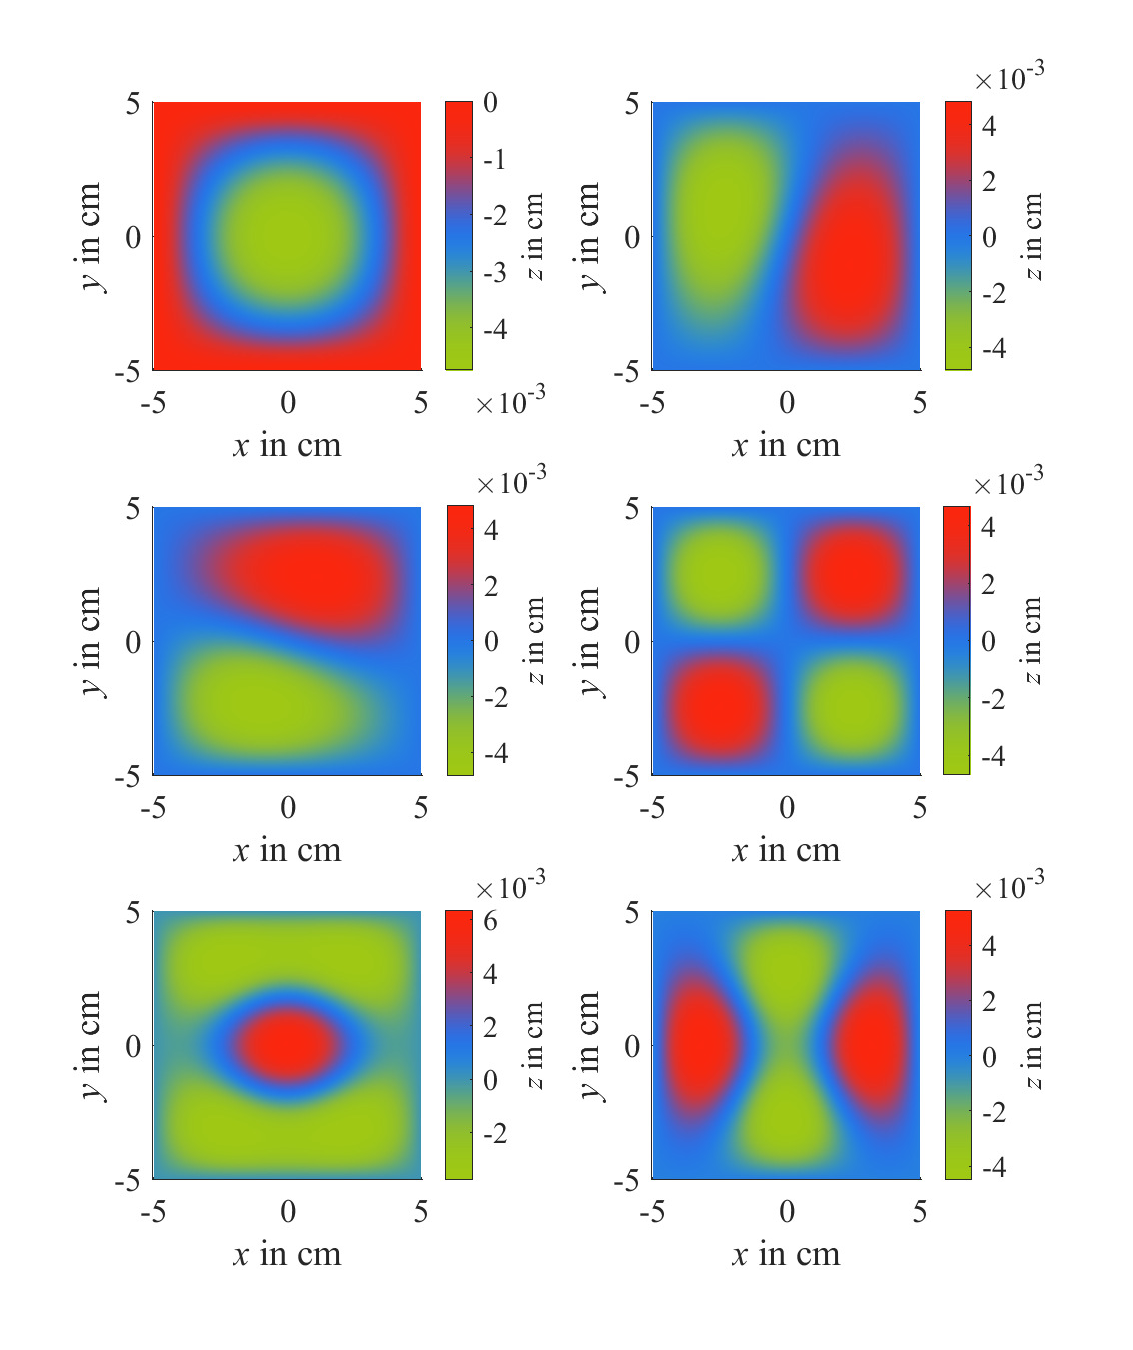
\includegraphics[width=\textwidth]{Chladni_Quadrat.pdf}
  \caption[Chladnische Klangfiguren f�r eine quadratische Fl�che.]
  {Chladnische Klangfiguren f�r eine quadratische Fl�che. Dargestellt sind die
    numerischen L�sungen f�r die ersten sechs Eigenschwingungen der
    elastischen Fl�che.}
  \label{abb:kontmech_ChladniQuadrat}
\end{figure}

\newpage
\begin{figure}
  \centering
  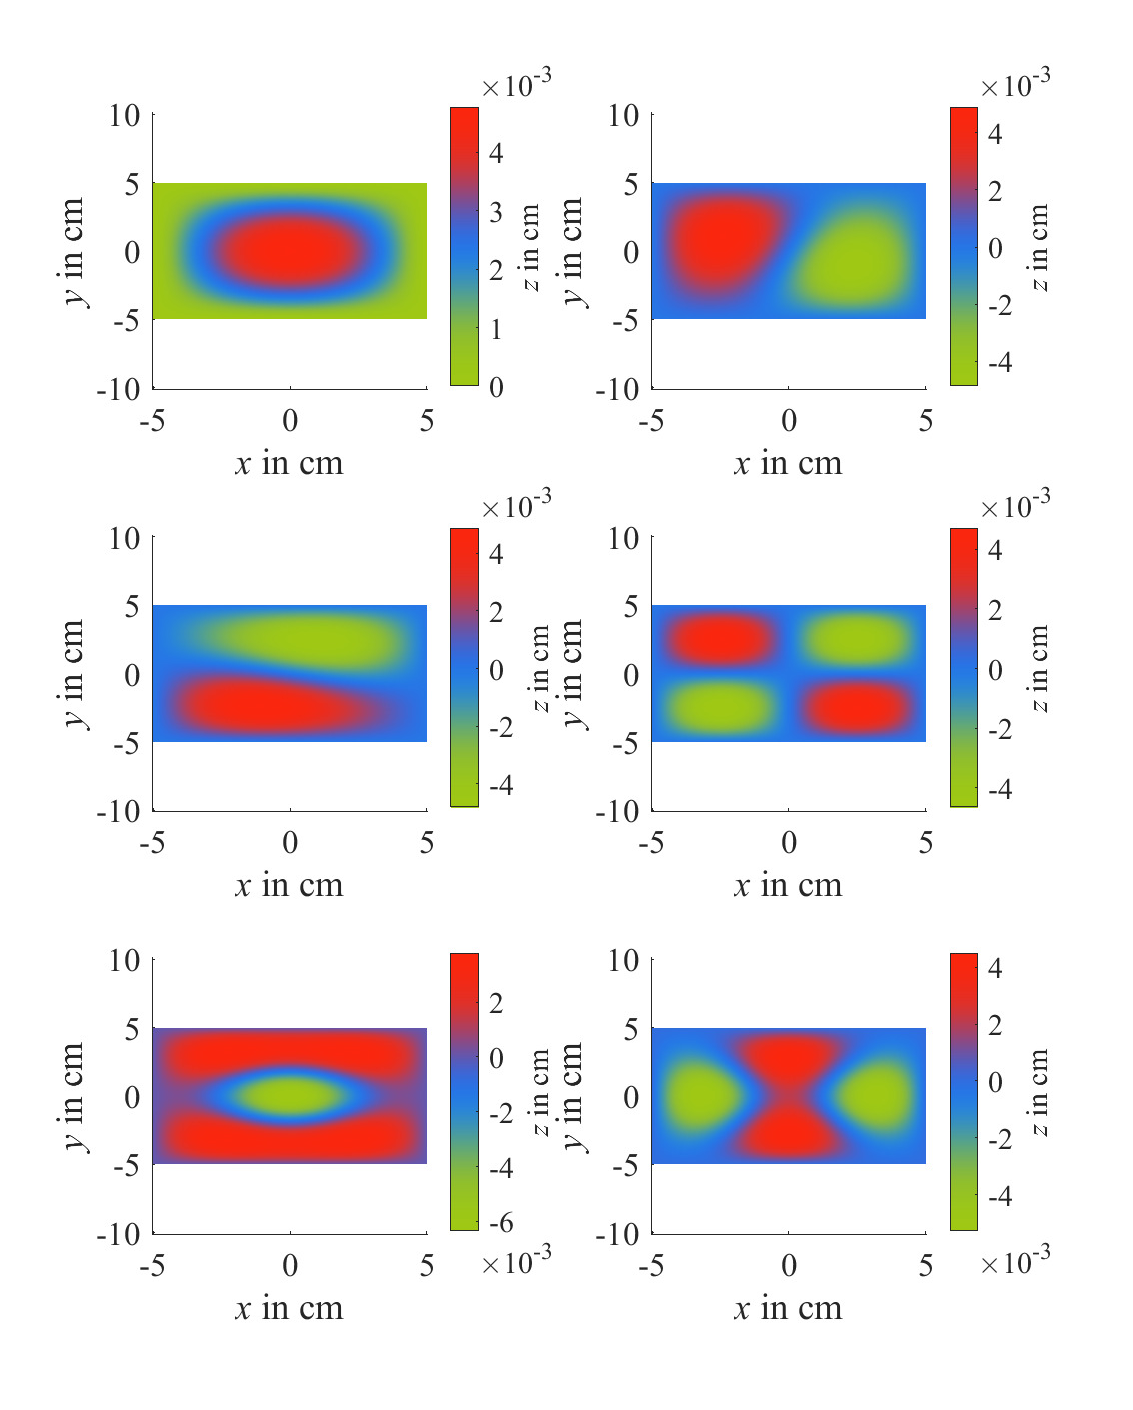
\includegraphics[width=\textwidth]{Chladni_Rechteck.pdf}
  \caption[Chladnische Klangfiguren f�r eine rechteckige Fl�che.]
  {Chladnische Klangfiguren f�r eine rechteckige Fl�che. Dargestellt sind die
    numerischen L�sungen f�r die ersten sechs Eigenschwingungen der
    elastischen Fl�che.}
  \label{abb:kontmech_ChladniRechteck}
\end{figure}

\end{sol} 
\textcolor{blue} {$\rightarrow$ zur} \probref{kontmech_Chladni}.\\
\noindent\rule[1ex]{\textwidth}{0.5pt}  \newpage  \clearpage

% ----------------------------------------------------------------------------------------------------------
% ----------------------------------------------------------------------------------------------------------

\newpage
\subsection{�bungen zu Wellen}

\medskip

% ----------------------------------------------------------------------------------------------------------

%-----------------------------------------------------------------------------------------------------------

\begin{sol}{prob:kontmech_Dispersion}\label{lsg:kontmech_Dispersion} %�bung24
\textbf{Wellenausbreitung und Dispersion}\\

Die L�sung ist im Detail im \mscr{} \mlkontmechref{DispersionWelle.m} hinterlegt.
  \begin{figure}
    \centering
    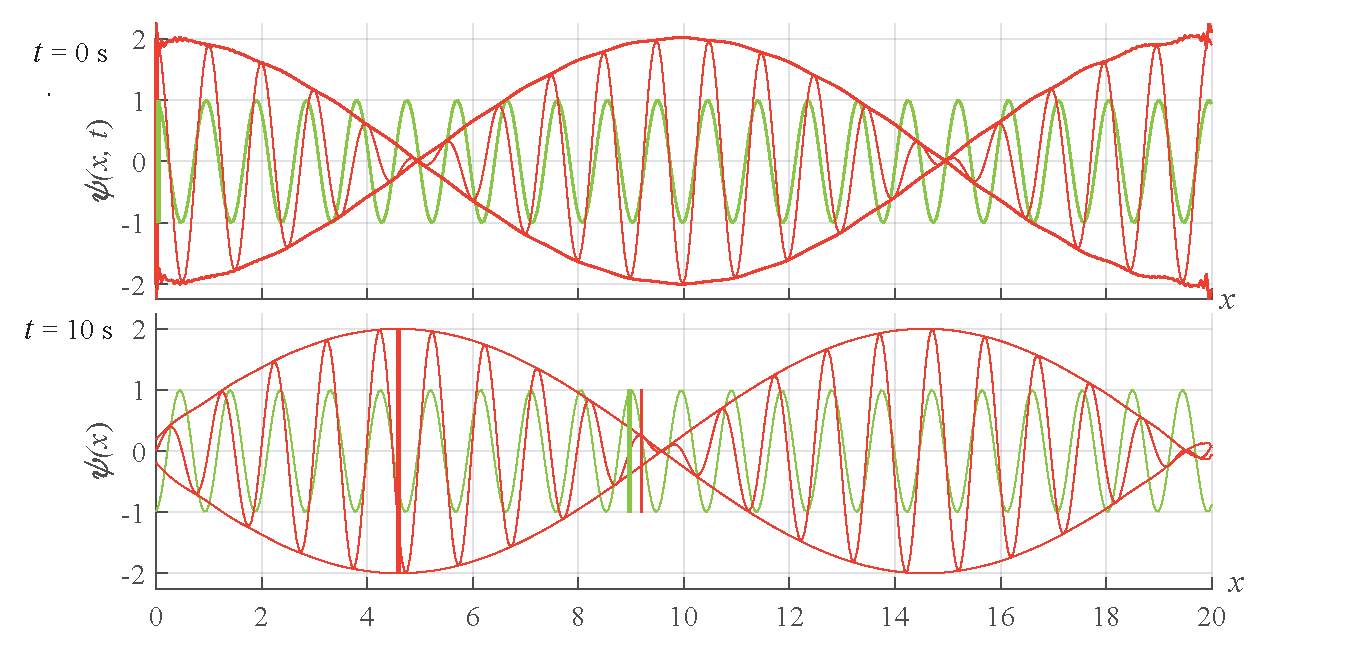
\includegraphics[width=0.85\textwidth]{DispersionWelle.pdf}
    \caption[Ausbreitung einer �berlagerung von zwei Wellen �hnlicher Wellenl�nge.]
    {Ausbreitung einer �berlagerung von zwei Wellen �hnlicher Wellenl�nge. Die Wellenfunktion ist zu zwei verschiedenen Zeitpunkten gezeigt. Deutlich sind die Unterschiede von Phasen- und Gruppengeschwindigkeit erkennbar, der blaue Balken zeigt die Fortbewegung der Einh�llenden und der gr�ne Balken die der Phase. Bei den gew�hlten Parametern liegt normale Dispersion vor mit $v_\text{gr} = 0.5\, v_\text{ph}$.}
    \label{abb:kontmech_Dispersion01}
  \end{figure}
  \begin{figure}
    \centering
    \includegraphics[width=0.85\textwidth]{DispersionWellenPaket.pdf}
    \caption[Ausbreitung eines Wellenpakets.]
    {Ausbreitung eines Wellenpakets aus der �berlagerung von 50 einzelnen Wellen.}
    \label{abb:kontmech_Dispersion02}
  \end{figure}

\end{sol} 
\textcolor{blue} {$\rightarrow$ zur} \probref{kontmech_Dispersion}.\\
\noindent\rule[1ex]{\textwidth}{0.5pt}  \newpage  \clearpage

%-----------------------------------------------------------------------------------------------------------

\begin{sol}{prob:kontmech_Dispersion2}\label{lsg:kontmech_Dispersion2} %�bung25
\textbf{Ausbreitung eines Wellenpakets unter Dispersion}\\ \\

Die L�sung ist im Detail im \mscr{} \mlkontmechref{DispersionWellenpaket.m} hinterlegt.
Im einzelnen erfolgte die L�sung in folgenden Schritten:

\begin{enumerate}
\item Man berechne den Anfangsimpuls $\psi(x_n,t=0)$ im Ortsraum $0 \leq x_n \leq x_\text{end} =  \SI{4000}{\metre}, N_x = 40000,\,\delta x = \SI{0.1}{\metre}$. Aufgrund der zeitlichen Ausdehnung hat der Anfangsimpuls auch eine r�umliche Ausdehnung.
\item Man transformiere den Anfangsimpuls in den Fourier-Raum und erh�lt: $\Psi(k,t=0)$ F�r die Raumfrequenz bzw. Wellenzahl gilt: $0 \leq k_n \leq k_\text{end} = 2\pi / \delta x = 2\pi \SI{10}{\metre},\, N_k = 40000$.
\item Man bestimme die Phasengeschwindigkeiten $v_{\text{Ph},n}(k_n)$ und die Kreisfrequenzen $\omega_n(k_n)$ als Funktion der Wellenzahlen Dabei benutze man die gegebene Dispersionsrelation $v_ph(k)$.
\item Die Ausbreitung durch das Medium wird als zeitliche Evolution im Frequenzraum mit der Filterfunktion $\mathrm{exp}(\im \omega_n\,t_\text{mess})$ beschrieben, worin $t_\text{mess}$ die Zeit der Propagation durch das Medium ist.
\item Man multipliziere $\mathrm{exp}(\im \omega_n\,t_\text{mess})$ mit $\Psi(k_n,t=0)$ und bilde die R�cktransformation, was schlie�lich $\psi(x_n, t=t_\text{mess})$ ergibt.
\item Man erkennt sehr sch�n, dass sich das Wellenpaket bei der Ausbreitung im dispersiven Medium verbreitert (Energie bleibt konstant aber Intensit�t verringert sich) und als ganzes mit der Gruppengeschwindigkeit vorw�rts bewegt.
\end{enumerate}

  \begin{figure}
    \centering
    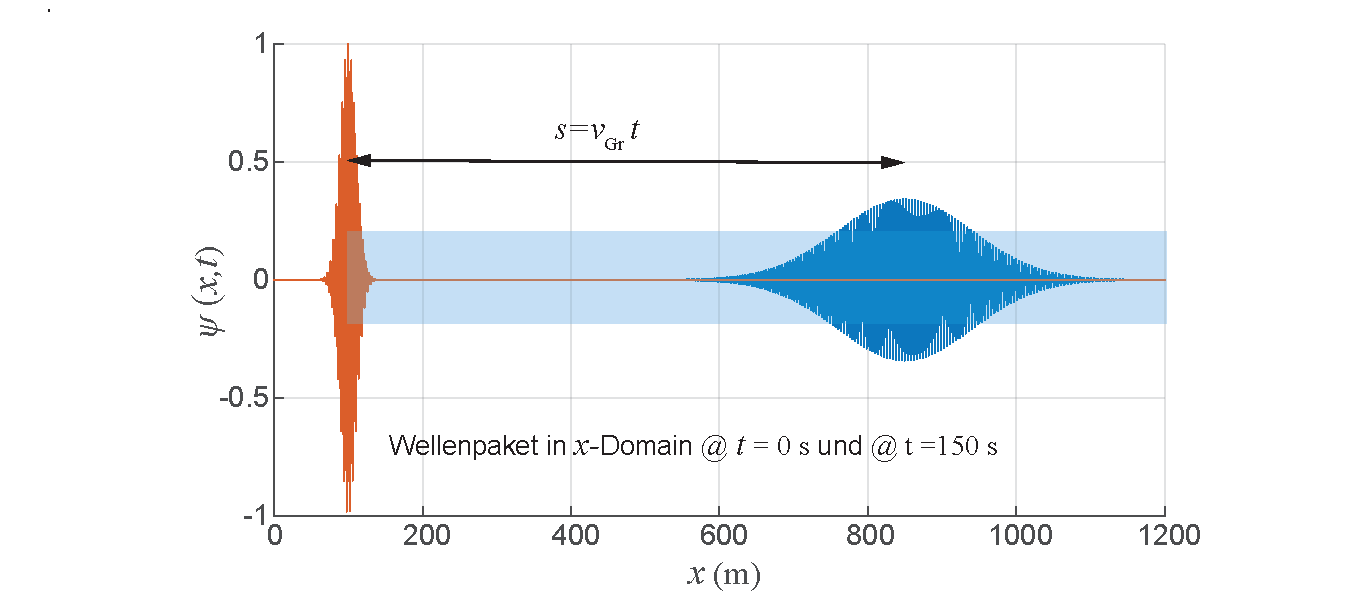
\includegraphics[width=\textwidth]{DispersionGaussWellenpaket.pdf}
    \caption[Ausbreitung eines Gau�-Wellenpakets in einem dispersivem Medium.]
    {Ausbreitung eines Gau�-Wellenpakets in einem dispersivem Medium. Man erkennt deutlich die Verbreiterung (das Auseinanderflie�en) des Wellenpakets, das sich selbst mit der Gruppengeschwindigkeit $v_\text{Gr}$ im Medium ausbreitet.}
    \label{abb:kontmech_DispersionGauss01}
  \end{figure}

Hinweise:
\begin{itemize}
	\item Die dargestellte Berechnung kann auch erfolgen, indem man von einer zeitlichen Anfangsverteilung ausgeht und dann im Fourier-Raum die Propagation durch das Medium betrachtet. Der entsprechende Propagator enth�lt dann die L�nge des Mediums als Messgr��e (Zusatz�bung).
	\item Wie erw�hnt liegt die Grundlage der beschriebenen Vorgehensweise in der Linearit�t der Wellengleichung. F�r den Gau�-f�rmigen Impuls kann man die L�sung auch analytisch berechnen (Zusatz�bung). Wir werden das im Band Optik an Hand der Wellengleichung f�r Lichtimpulse behandeln.
	\item Laut Vorgabe haben wir eine lineare Abh�ngigkeit der Phasengeschwindigkeit von der Wellenzahl, die Gruppengeschwindigkeit ist somit eine Konstante und zeigt selbst keine Dispersion. Im Allgemeinen zeigt auch die Gruppengeschwindigkeit eine Dispersion, n�mlich dann, wenn 
		\begin{align*}
			\frac{\d v_\text{Gr}}{\d k} = \frac{\d^2 \omega}{\d k^2} \neq 0\,.
		\end{align*}
	Man hat dann sogenannte Gruppengeschwindigkeitsdispersion vorliegen, die besonders bei optischen Impulsen in Fasern relevant zu ber�cksichtigen ist. Wir werden uns auch damit im Band Optik besch�ftigen.
\end{itemize}


  \begin{figure}
    \centering
    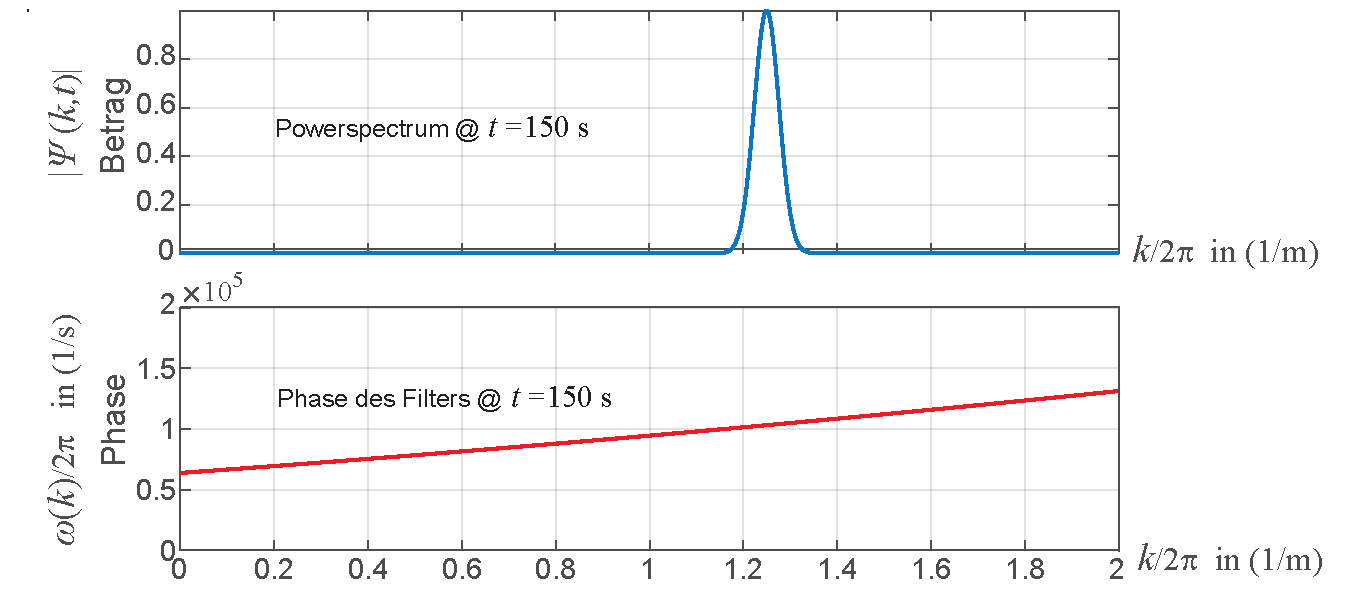
\includegraphics[width=\textwidth]{DispersionGaussWellenpaket02.pdf}
    \caption[Leistungsspektrum eines Gau�-Wellenpakets und Filtercharakteristik eines dispersiven Mediums.]
    {Leistungsspektrum eines Gau�-Wellenpakets und Filtercharakteristik eines dispersiven Mediums.}
    \label{abb:kontmech_DispersionGauss02}
  \end{figure}



\end{sol} 
\textcolor{blue} {$\rightarrow$ zur} \probref{kontmech_Dispersion2}.\\
\noindent\rule[1ex]{\textwidth}{0.5pt}  \newpage  \clearpage

%-----------------------------------------------------------------------------------------------------------

\begin{sol}{prob:kontmech_soliton1}\label{lsg:kontmech_soliton1} %�bung26
\textbf{Solitonen I}\index{Solitonen}\\ \\

Einerseits ist f�r die Korteweg-de-Vries-Gleichung
\begin{equation}
  \frac{\partial \psi}{\partial t} + 6\,\psi\,\frac{\partial \psi}{\partial x}
  + \frac{\partial^3 \psi}{\partial x^3} = 0
  \tag{\ref{eq:kontmech_soliton01}}
\end{equation}
mit
\begin{align}
    \psi(x,t) = \frac{c}{2}\;\sech^2\lek \frac{\sqrt{c}}{2}\;\lk x-ct \rk \rek
  \tag{\ref{eq:kontmech_soliton02}}
\end{align}
eine Einzel-Soliton-L�sung\footnote{Dar�ber hinaus gibt es weitere analytische
  L�sungen, z.B. f�r $N$ Solitonen, die jedoch �ber unsere Betrachtung
  hinausgehen.} analytisch bekannt, andererseits haben wir mit den numerischen
Methoden, partielle Differentialgleichungen zu l�sen, eine M�glichkeit an der
Hand, diese L�sungen genauer zu untersuchen und F�lle zu konstrieren, die
dar�ber hinausgehen. Dies alles wollen wir in dieser L�sung tun.

\begin{enumerate}
\item Zun�chst stellen wir die Soliton-L�sungen \eqref{eq:kontmech_soliton02} 
  dar. Ein Beispiel mit dem Parameter $c=1$ ist in
  \figref{kontmech_KdV1Soliton} gegeben. Eine solche L�sung ver�ndert,
  wie es von einem Soliton zu erwarten ist, ihre Form nicht. Die L�sung
  wandert in der Zeit zu gr��eren Orten $x$, was die einzige erkennbare
  Zeitwenticklung darstellt.

  \begin{figure}
    \centering
    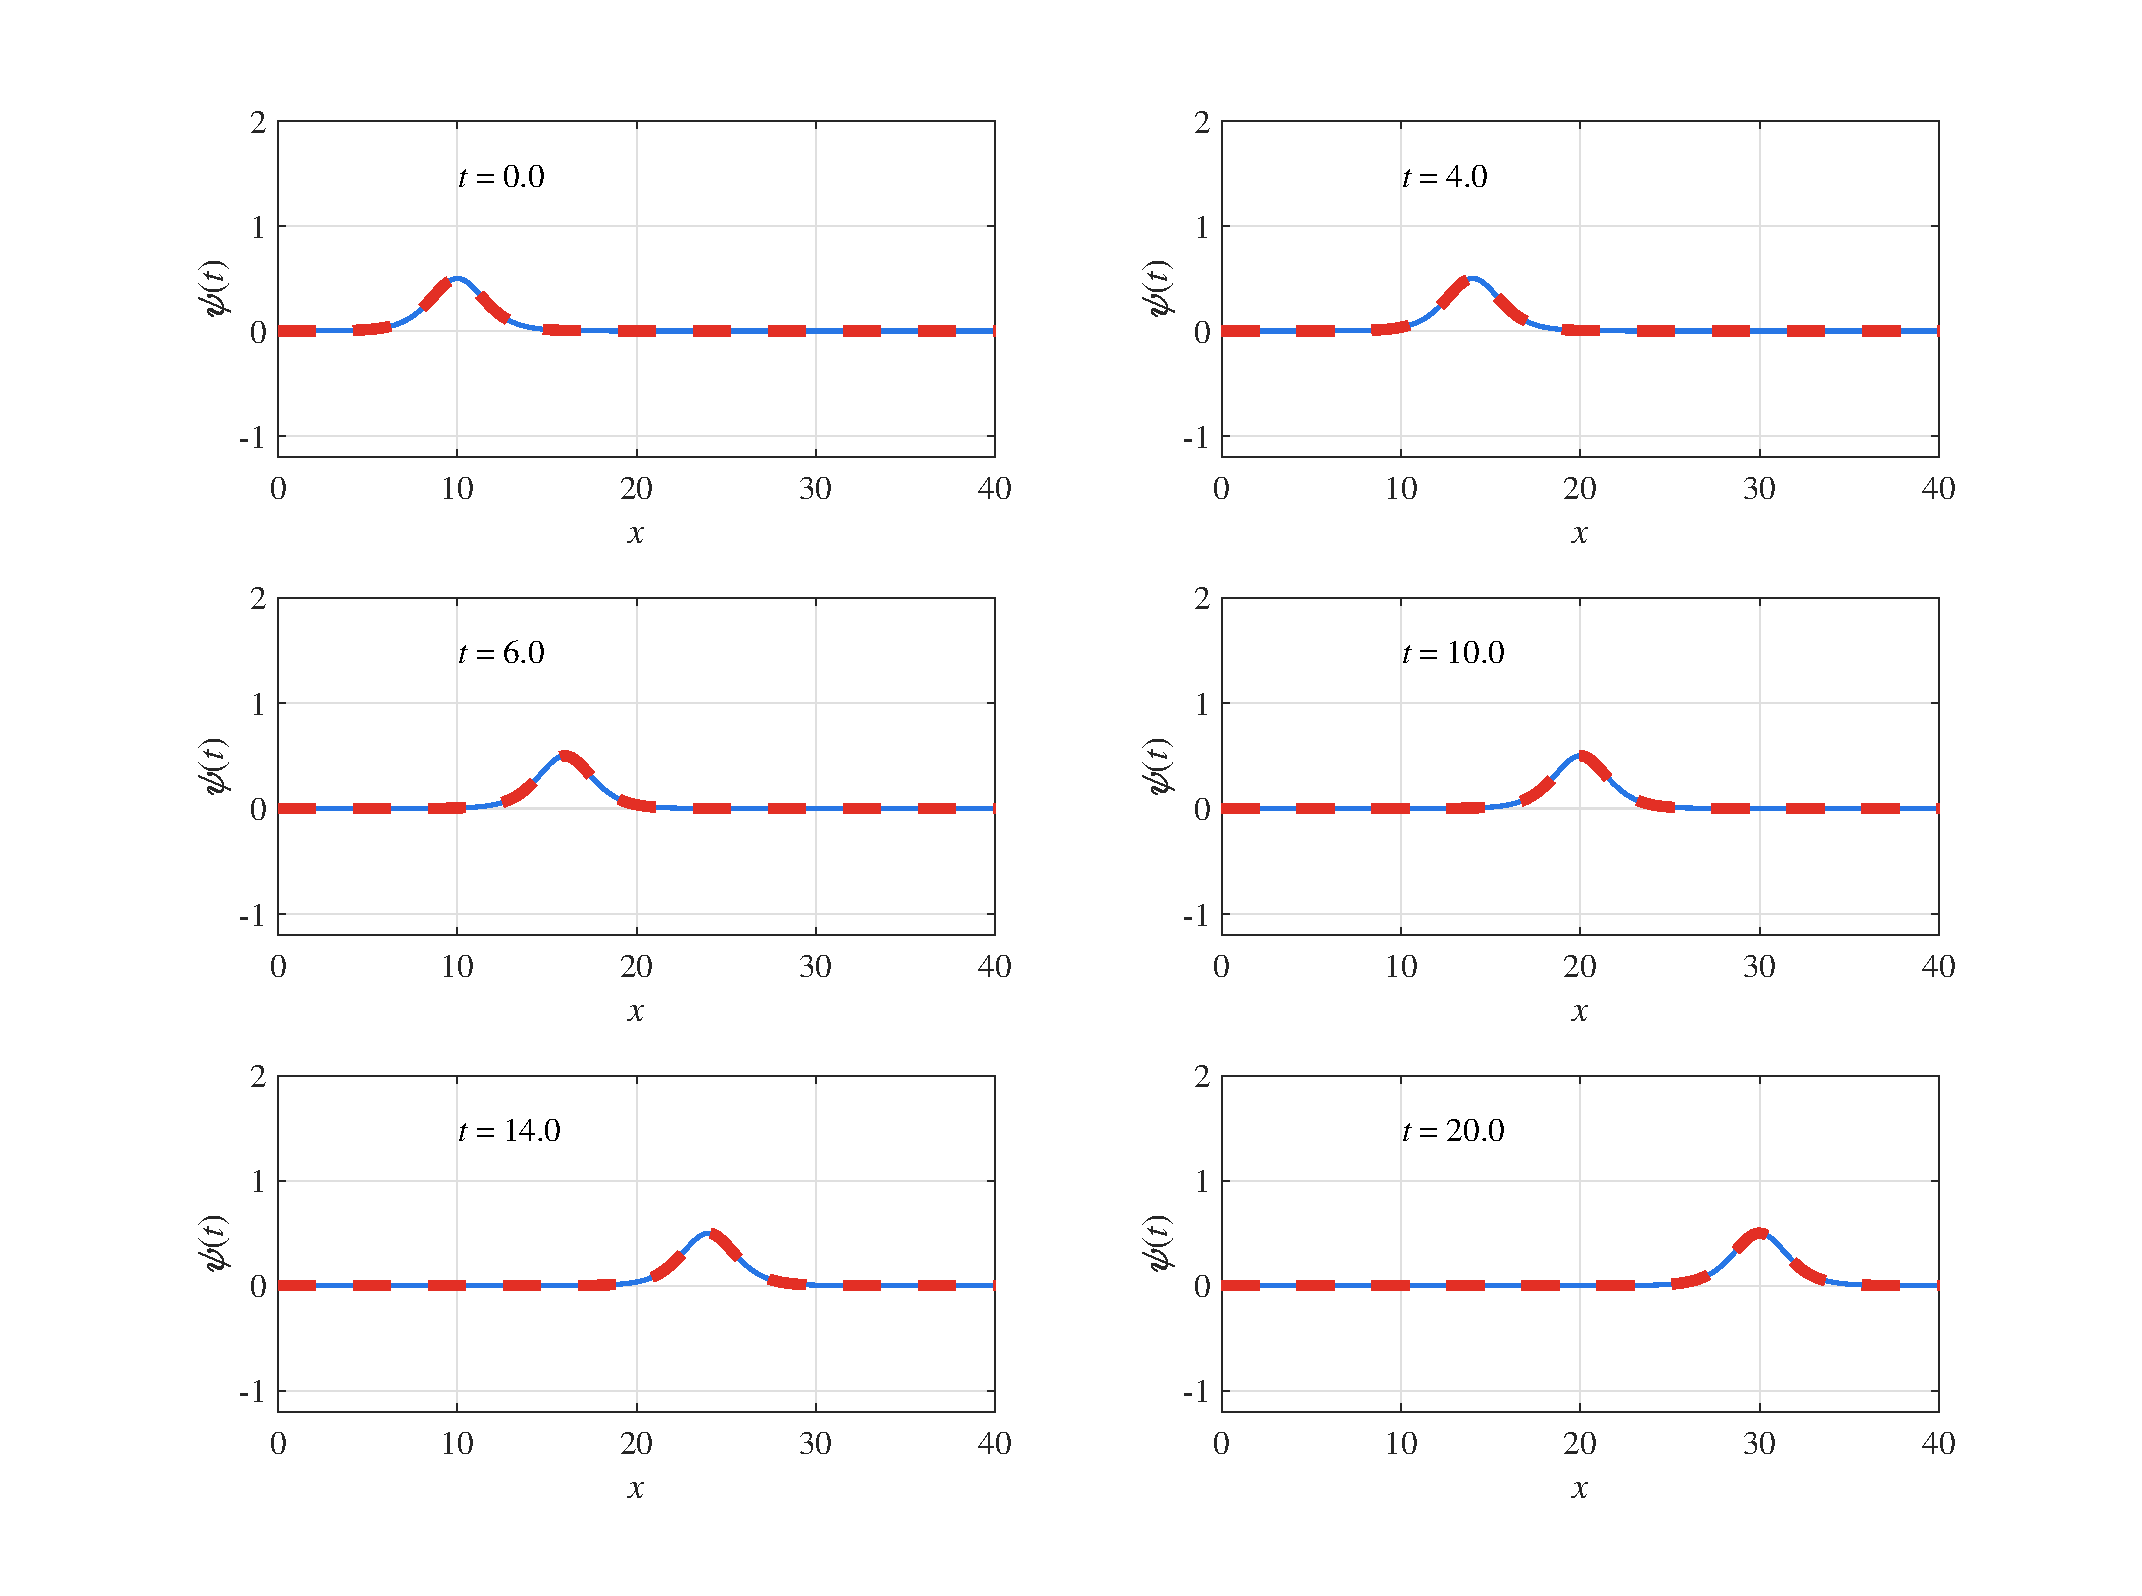
\includegraphics[width=\textwidth]{KdV1Soliton.pdf}
    \caption[Ausbreitung einer Soliton-L�sung der Korteweg-de-Vries-Gleichung.]
    {Ausbreitung einer einzelnen Soliton-L�sung der Korteweg-de-Vries-Gleichung
      nach Gleichung \eqref{eq:kontmech_soliton02} f�r $c = 1$ (blaue,
      durchgezogene Linie). Die Stabilit�t der Form ist erkennbar, w�hrend
      sich das Soliton nach rechts bewegt. Eine numerische L�sung der
      partiellen Differentialgleichung \eqref{eq:kontmech_soliton01} f�hrt f�r
      dieselben Startwerte zum selben Ergebnis (rot gestrichelte Linie).}
    \label{abb:kontmech_KdV1Soliton}
  \end{figure}
  
  Verschiedene L�sungen f�r die Parameter $c = 0.5, 1, 2, 3$ werden in
  \figref{kontmech_KdVSolitonVergleichc} miteinander verglichen. Als erstes
  f�llt auf, dass alle dieselbe grundlegende Form haben. Dies �berrascht nicht
  weiter, da sie alle der Form \eqref{eq:kontmech_soliton02} entsprechen.
  Genauso kann man aus der Gleichung ablesen, dass ein gr��erer Wert von $c$
  zu einem h�heren Maximum von $ \psi$ f�hrt, die Funktion daf�r um das Maximum
  herum schneller abf�llt. Dies findet sich alles in der Darstellung wieder.
  Dar�ber hinaus erkennt man die Stabilit�t der Form f�r alle Werte von
  $c$. Da $c$ die Bedeutung einer Geschwindigkeit hat, breiten die verschiedenen
  L�sungen sich unterschiedlich schnell nach rechts aus. 

  \begin{figure}
    \centering
    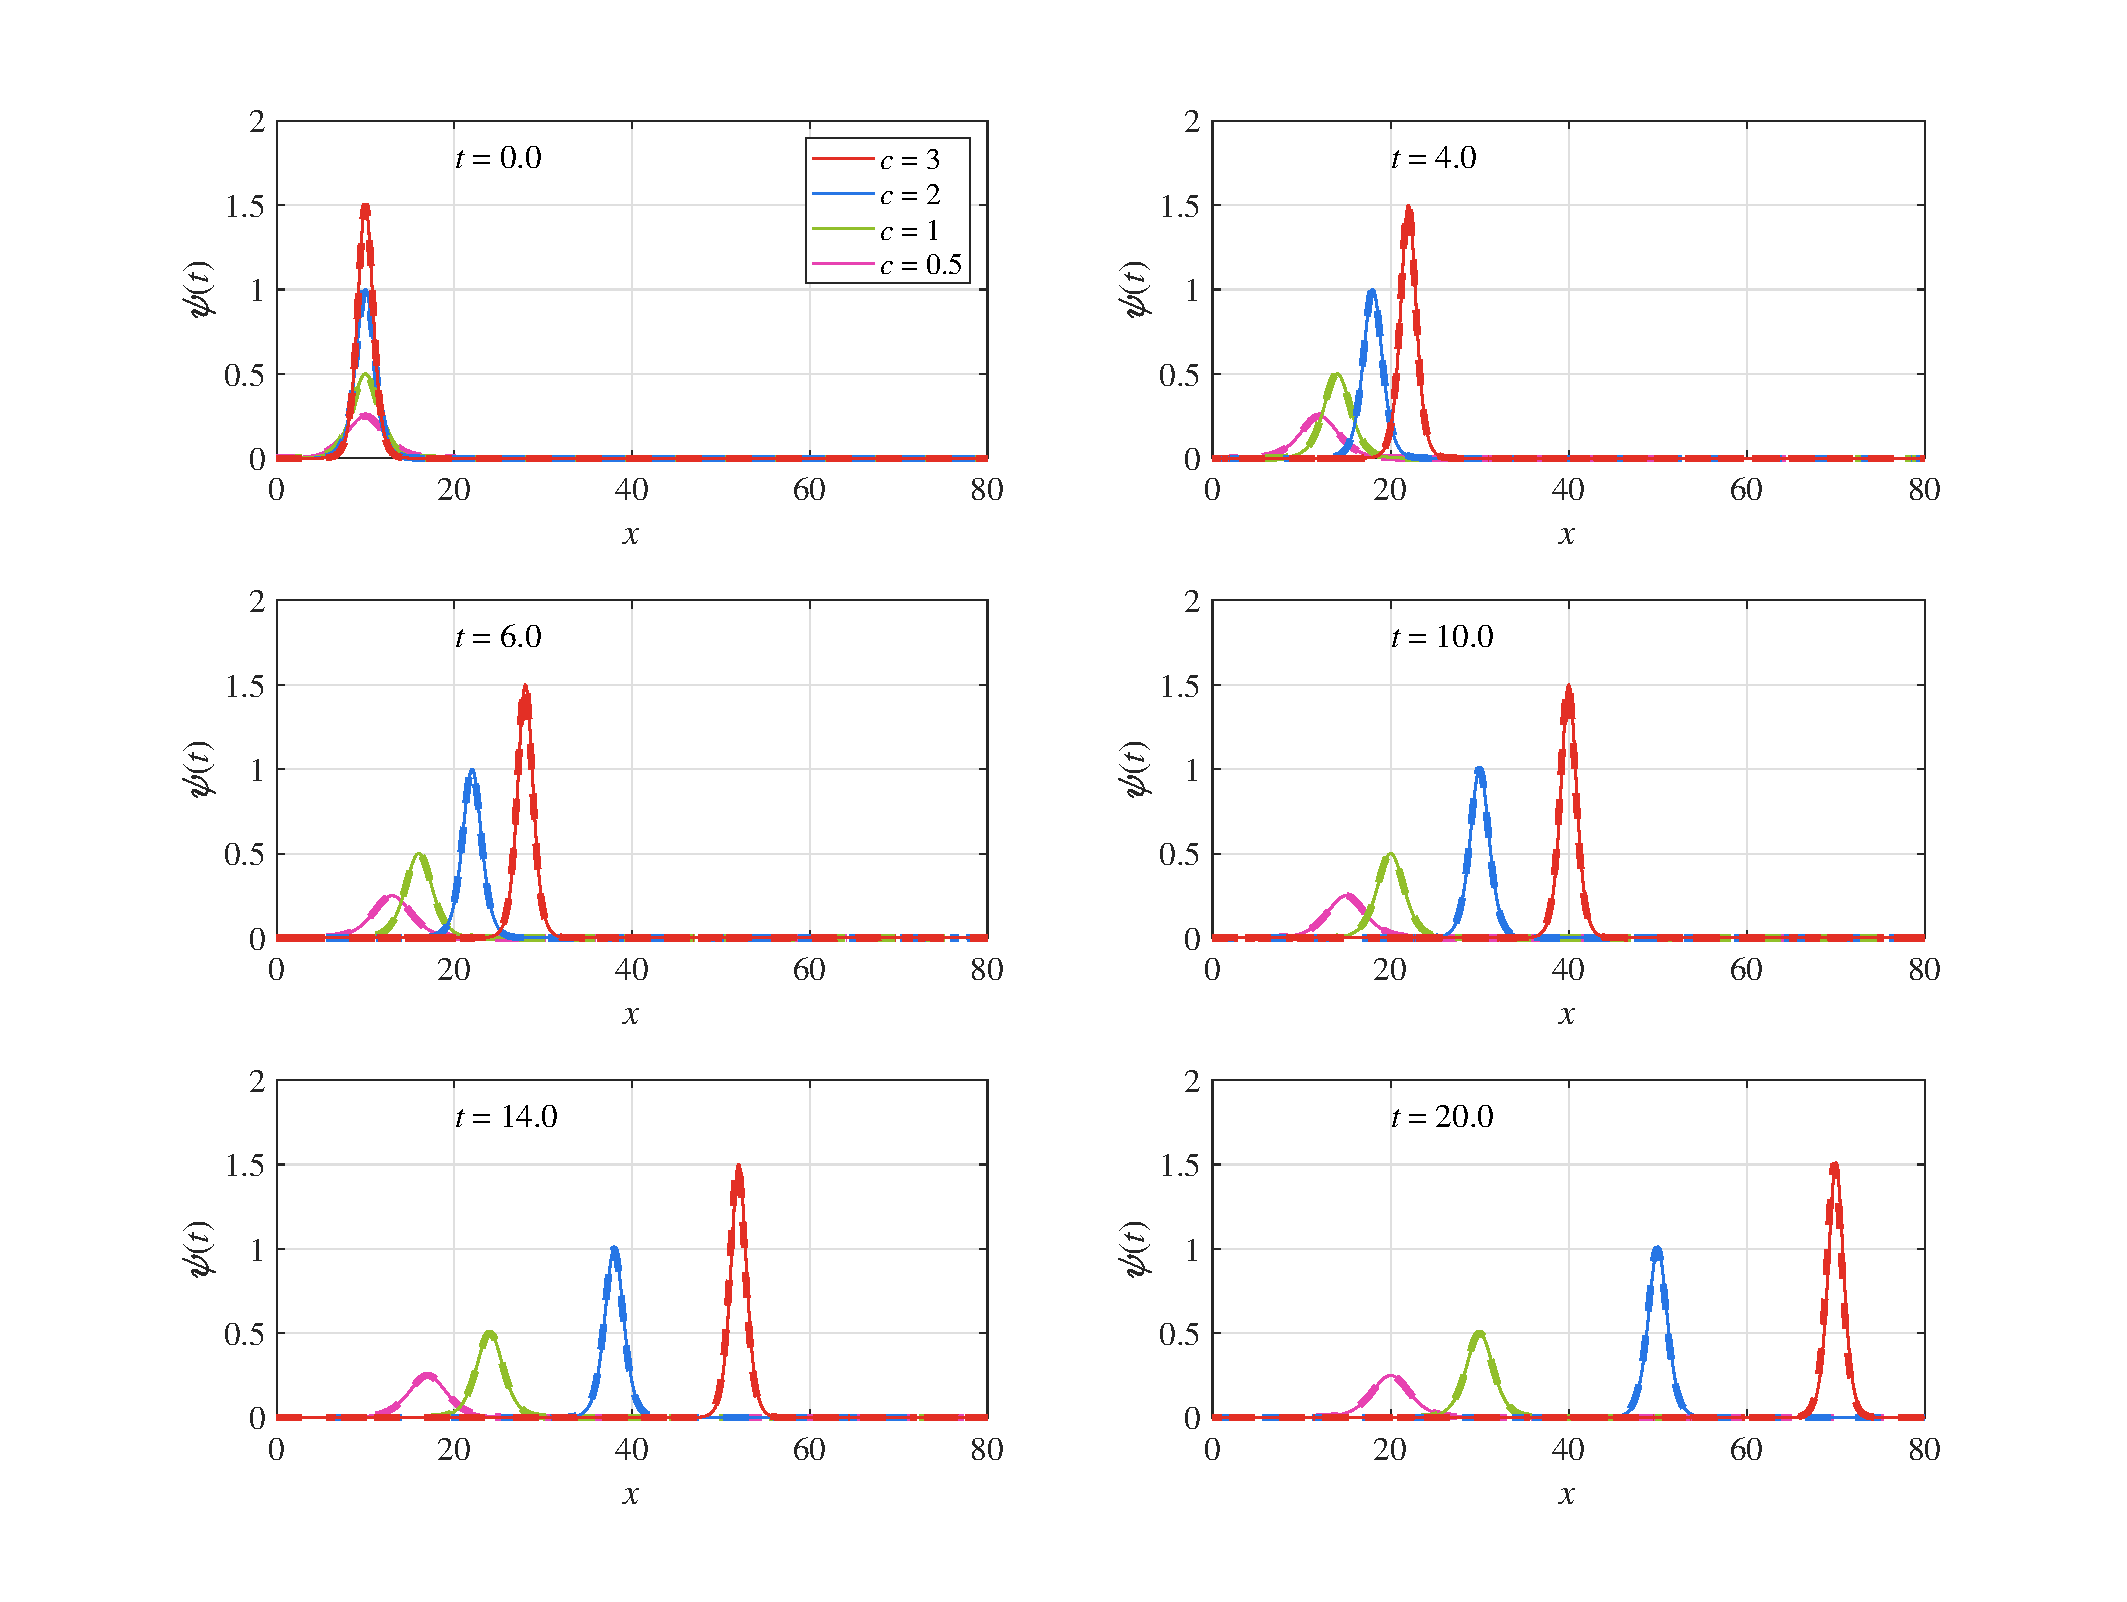
\includegraphics[width=\textwidth]{KdVSolitonVergleichc.pdf}
    \caption[Ausbreitung von Soliton-L�sung der Korteweg-de-Vries-Gleichung mit
    verschiedenem $c$.]
    {Ausbreitung mehrerer Soliton-L�sungen der Korteweg-de-Vries-Gleichung f�r
      die Geschwindigkeitsparamter $c = 0.5, 1, 2, 3$. Bei einer anderen
      Geschwindigkeit muss die L�sung der nichtlinearen Wellengleichung auch
      eine andere Gestalt annehmen, die jedoch derselben grundlegenden Form
      \eqref{eq:kontmech_soliton02} entspricht. Jede L�sung bleibt f�r sich
      stabil. Durchgezogene, d�nne Linien repr�sentieren die analytische
      L�sung \eqref{eq:kontmech_soliton02}, w�hrend gestrichelte, dicke Linien
      die zugh�rige numerische L�sung der partiellen Differentialgleichung
      \eqref{eq:kontmech_soliton01} darstellen.}
    \label{abb:kontmech_KdVSolitonVergleichc}
\end{figure}

\item Wir wollen nun zeigen, dass die Funktion \eqref{eq:kontmech_soliton02}
  tats�chlich eine L�sung der Korteweg-de-Vries-Gleichung
  \eqref{eq:kontmech_soliton01} ist. Dazu schreiben wir die L�sung
  zun�chst als 
  \begin{align}
    \psi(x,t) = \frac{c}{2}\;\sech^2\lek \frac{\sqrt{c}}{2}\;\lk x-ct \rk \rek
    = \frac{c}{2} \frac{1}{\cosh^2\lek \frac{\sqrt{c}}{2}\;\lk x-ct \rk \rek}
  \end{align}
  und bilden die Ableitungen, die wir f�r die weitere Rechnung ben�tigen:
  \begin{subequations}
    \allowdisplaybreaks
    \begin{align}
      \frac{\partial \psi(x,t)}{\partial t}
      &= \frac{c^{5/2}}{2} \frac{\sinh\lek \frac{\sqrt{c}}{2}\;\lk x-ct \rk
        \rek}{\cosh^3\lek \frac{\sqrt{c}}{2}\;\lk x-ct \rk \rek} \; ,\\
      \frac{\partial \psi(x,t)}{\partial x}
      &= -\frac{c^{3/2}}{2} \frac{\sinh\lek \frac{\sqrt{c}}{2}\;\lk x-ct \rk
        \rek}{\cosh^3\lek \frac{\sqrt{c}}{2}\;\lk x-ct \rk \rek} \; ,\\
      \frac{\partial^2 \psi(x,t)}{\partial x^2}
      &= \frac{c^{2}}{4} \left \{ -\frac{1}{\cosh^2\lek \frac{\sqrt{c}}{2}\;
        \lk x-ct \rk \rek} 
        +3 \frac{\sinh^2\lek \frac{\sqrt{c}}{2}\;\lk x-ct \rk
        \rek}{\cosh^4\lek \frac{\sqrt{c}}{2}\;\lk x-ct \rk \rek} \right \} \; ,
      \\
      \frac{\partial^3 \psi(x,t)}{\partial x^3}
      &= \frac{c^{5/2}}{8} \left \{ 8\frac{\sinh\lek \frac{\sqrt{c}}{2}\;
        \lk x-ct \rk \rek}{\cosh^3\lek \frac{\sqrt{c}}{2}\;\lk x-ct \rk \rek} 
       -12 \frac{\sinh^3\lek \frac{\sqrt{c}}{2}\;\lk x-ct \rk
        \rek}{\cosh^5\lek \frac{\sqrt{c}}{2}\;\lk x-ct \rk \rek} \right \}
        \; .
    \end{align}
  \end{subequations}
  Setzt man diese Ableitungen in die Korteweg-de-Vries-Gleichung ein, so
  erh�lt man
  \begin{multline*}
    \frac{c^{5/2}}{2} \frac{\sinh\lek \frac{\sqrt{c}}{2}\;\lk x-ct \rk
      \rek}{\cosh^3\lek \frac{\sqrt{c}}{2}\;\lk x-ct \rk \rek}
    - 6 \; \frac{c}{2} \frac{1}{\cosh^2\lek \frac{\sqrt{c}}{2}\;\lk x-ct \rk
      \rek} \cdot \frac{c^{3/2}}{2} \frac{\sinh\lek \frac{\sqrt{c}}{2}\;
      \lk x-ct \rk \rek}{\cosh^3\lek \frac{\sqrt{c}}{2}\;\lk x-ct \rk \rek}
    \\
    + \frac{c^{5/2}}{8} \left \{ 8\frac{\sinh\lek \frac{\sqrt{c}}{2}\;
        \lk x-ct \rk \rek}{\cosh^3\lek \frac{\sqrt{c}}{2}\;\lk x-ct \rk \rek} 
      -12 \frac{\sinh^3\lek \frac{\sqrt{c}}{2}\;\lk x-ct \rk
        \rek}{\cosh^5\lek \frac{\sqrt{c}}{2}\;\lk x-ct \rk \rek} \right \}
    = 0 \; .
  \end{multline*}
  Um diese Terme besser vergleichen zu k�nnen, multiplizieren wir alle
  mit $4/c^{5/2}$ und bringen sie auf den Hauptnenner
  $\cosh^5\lek \frac{\sqrt{c}}{2}\;\lk x-ct \rk \rek$,
  \begin{multline*}
    2\; \frac{\sinh\lek \frac{\sqrt{c}}{2}\;\lk x-ct \rk \rek \;
      \cosh^2\lek \frac{\sqrt{c}}{2}\;\lk x-ct \rk \rek}
    {\cosh^5\lek \frac{\sqrt{c}}{2}\;\lk x-ct \rk \rek}
    - 6 \; \frac{\sinh\lek \frac{\sqrt{c}}{2}\;\lk x-ct \rk \rek}
    {\cosh^5\lek \frac{\sqrt{c}}{2}\;\lk x-ct \rk \rek} \\
    + 4 \frac{\sinh\lek \frac{\sqrt{c}}{2}\;\lk x-ct \rk \rek \;
      \cosh^2\lek \frac{\sqrt{c}}{2}\;\lk x-ct \rk \rek}
    {\cosh^5\lek \frac{\sqrt{c}}{2}\;\lk x-ct \rk \rek} 
    -6 \frac{\sinh^3\lek \frac{\sqrt{c}}{2}\;\lk x-ct \rk
        \rek}{\cosh^5\lek \frac{\sqrt{c}}{2}\;\lk x-ct \rk \rek} 
    = 0 \; .
  \end{multline*}
  Die linke Seite l�sst sich zusammenfassen zu
  \begin{multline*}
    \frac{6\; \sinh\lek \frac{\sqrt{c}}{2}\;\lk x-ct \rk \rek \left \{
          \cosh^2\lek \frac{\sqrt{c}}{2}\;\lk x-ct \rk \rek
          - \sinh^2\lek \frac{\sqrt{c}}{2}\;\lk x-ct \rk \rek \right \} }
    {\cosh^5\lek \frac{\sqrt{c}}{2}\;\lk x-ct \rk \rek}
    - 6 \; \frac{\sinh\lek \frac{\sqrt{c}}{2}\;\lk x-ct \rk \rek}
    {\cosh^5\lek \frac{\sqrt{c}}{2}\;\lk x-ct \rk \rek} \\
    = \frac{6\; \sinh\lek \frac{\sqrt{c}}{2}\;\lk x-ct \rk \rek}
    {\cosh^5\lek \frac{\sqrt{c}}{2}\;\lk x-ct \rk \rek}
    - 6 \; \frac{\sinh\lek \frac{\sqrt{c}}{2}\;\lk x-ct \rk \rek}
    {\cosh^5\lek \frac{\sqrt{c}}{2}\;\lk x-ct \rk \rek} 
    = 0 \; ,
  \end{multline*}
  und erf�llt somit die rechte Seite. Damit ist gezeigt, dass die Funktion
  \eqref{eq:kontmech_soliton02} eine L�sung der Korteweg-de-Vries-Gleichung
  \eqref{eq:kontmech_soliton01} darstellt.
  
\item Wir wollen nun noch zeigen, dass die Summe $\psi_1+\psi_2$ von zwei
  L�sungen $\psi_1$ und $\psi_2$ der KdV-Gleichung \iA selbst keine
  L�sung darstellt. Dies ist eine Eigenschaft nichtlinearer
  Differentialgleichungen.

  Wir setzen zun�chst die Summe in die KdV-Gleichung ein und erhalten
  \begin{align*}
    \frac{\partial}{\partial t} \lk \psi_1 + \psi_2 \rk
    + 6\,\lk\psi_1 + \psi_2 \rk\,\frac{\partial }{\partial x} \lk \psi_1
    + \psi_2 \rk   
    + \frac{\partial^3}{\partial x^3} \lk \psi_1 + \psi_2 \rk &= 0 \\
    \intertext{bzw.}
    \frac{\partial \psi_1}{\partial t} + \frac{\partial \psi_2}{\partial t}
    + 6\,\lk\psi_1 + \psi_2 \rk\, \lk \frac{\partial \psi_1}{\partial x}
     + \frac{\partial \psi_2}{\partial x} \rk
    + \frac{\partial^3 \psi_1}{\partial x^3}
    + \frac{\partial^3 \psi_2}{\partial x^3} &= 0 \; .
  \end{align*}
  Diese Terme sortieren wir neu zu
  \begin{equation}
    \left \{ \frac{\partial \psi_1}{\partial t} + 6 \, \psi_1 \,
      \frac{\partial \psi_1}{\partial x} + \frac{\partial^3 \psi_1}
      {\partial x^3} \right \}
    + \left \{ \frac{\partial \psi_2}{\partial t} + 6 \, \psi_2 \,
      \frac{\partial \psi_2}{\partial x} + \frac{\partial^3 \psi_2}
      {\partial x^3} \right \}
    + 6\,\psi_1 \, \frac{\partial \psi_2}{\partial x} 
    + 6\,\psi_2 \, \frac{\partial \psi_1}{\partial x} = 0 \; .
  \end{equation}
  Da $\psi_1$ und $\psi_2$ nach Voraussetzung L�sungen der KdV-Gleichung
  sind, verschwinden die beiden geschweiften Klammern und es m�sste gelten,
  dass
  \begin{subequations}
    \begin{align}
      6\,\psi_1 \, \frac{\partial \psi_2}{\partial x} 
      + 6\,\psi_2 \, \frac{\partial \psi_1}{\partial x}
      &\overset{!}{=} 0 \label{eq:kontmech_KdVSumme1} \\
      \intertext{oder}
      \frac{1}{\psi_1} \, \frac{\partial \psi_1}{\partial x} 
      &= -\frac{1}{\psi_2} \, \frac{\partial \psi_2}{\partial x} 
    \end{align}
  \end{subequations}
  Es ist sicher einsichtig, dass das \iA nicht erf�llt ist,
  da diese Gleichung f�r alle Werte $x$ und $t$ erf�llt sein m�sste. Man
  kann einen Widerspruch jedoch auch deutlicher zeigen, denn die Gleichung
  m�sste auch f�r $\psi_1 = \psi_2$ gelten. In diesem Spezialfall kommen wir
  allerdings auf
  \begin{align}
    \frac{1}{\psi_1} \, \frac{\partial \psi_1}{\partial x} 
    &= -\frac{1}{\psi_1} \, \frac{\partial \psi_1}{\partial x} \notag \\
    \intertext{oder f�r $\psi_1 \neq 1$, was die L�sungen
    \eqref{eq:kontmech_soliton02} erf�llen,}
    \frac{\partial \psi_1}{\partial x} 
    &= - \frac{\partial \psi_1}{\partial x} \;.
    \label{eq:kontmech_KdVSumme2}
  \end{align}
  Das stellt einen Widerspruch dar. Damit kann die Summe von zwei L�sungen der
  KdV-Gleichung im allgemeinem selbst keine L�sung sein.

\item M�chten wir die KdV-Gleichung numerisch mit der Methode der
  finiten Differenzen l�sen, so ben�tigen wir zun�chst Diskretisierungen
  der zugeh�rigen partiellen Ableitungen. Dazu orientieren wir uns an
  Kapitel \ref{kap:kontemch_finiteDifferenzen} und f�hren die
  ben�tigten Ableitungen ein:
  \begin{subequations}
    \begin{align}
      \frac{\partial \psi(x_i,t_j)}{\partial t}
      &= \frac{\psi(x_{i},t_{j+1}) - \psi(x_{i},t_{j-1})}{2\Delta t}  \; , \\
        \frac{\partial \psi(x,t)}{\partial x}
      &= \frac{\psi(x_{i+1},t_j) - \psi(x_{i-1},t_j)}{2\Delta x}  \; , \\
        \frac{\partial^3 \psi(x_i)}{\partial x_i^3}
      &= \frac{\psi(x_{i+2},t_j) -2 \psi(x_{i+1},t_j) +2 \psi(x_{i-1},t_j)
        - \psi(x_{i-2},t_j)}{2 \Delta x^3} \; .
    \end{align}
  \end{subequations}
  Wird dies in die Korteweg-de-Vries-Gleichung \eqref{eq:kontmech_soliton01}
  eingesetzt, so erh�lt man als Iterationsschritt f�r das numerische
  L�sen
  \begin{multline}
    \psi(x_i,t_{j+1}) = \psi(x_i,t_{j-1}) - 6 \, \frac{\Delta t}{\Delta x} \,
    \psi(x_i,t_j) \, \lk \psi(x_{i+1},t_j) - \psi(x_{i-1},t_j) \rk \\
    - \frac{\Delta t}{\Delta x^3} \, \lk \psi(x_{i+2},t_j)
    - 2 \psi(x_{i+1},t_j) +2 \psi(x_{i-1},t_j) - \psi(x_{i-2},t_j) \rk \; .
  \end{multline}

  Eine Implementierung dieses Finite-Differenzen-Ansatzes f�r die KdV-Gleichung
  kann in der \matlab{}-Datei \mlkontmechref{KdV01.m} gefunden werden.
  Das darin enthaltene Programm propagiert eine Soliton-L�sung, die mit
  der Anfangsbedingung aus \figref{kontmech_KdV1Soliton} identisch ist.
  In der Abbildung stellt die dick gestrichelte Linie die numerische L�sung
  mit der Finite-Differenzen-Methode dar. Man erkennt keinen Unterschied zur
  analytischen L�sung, was die hinreichende Qualit�t der numerischen L�sung
  demonstriert. Dies trifft auch auf weitere Geschwindigkeitsparameter $c$
  zu. Die \matlab{}-Datei \mlkontmechref{KdV02.m} l�st die KdV-Gleichung f�r
  alle Beispiele aus \figref{kontmech_KdVSolitonVergleichc} und stellt diese
  als dick gestrichelte Linien in der Abbildung dar.

  Die numerische L�sung gibt uns allerdings auch die M�glichkeit, zu
  veranschaulichen, wie sich die Summe aus zwei Solitonen in der Zeitentwicklung
  verh�lt. Wir wollen die Rechnung aus dem vorherigen Aufgabenteil durch
  numerische Beispiele unterlegen. Die \matlab{}-Datei \mlkontmechref{KdV03.m}
  enth�lt ein Programm, das die Summe aus zwei Solitonen propagiert. In
  \figref{kontmech_KdVSolitonSumme1} ist eine anf�ngliche �berlagerung von
  zwei einzelnen Soliton-L�sungen dargestellt.
  
  \begin{figure}
    \centering
    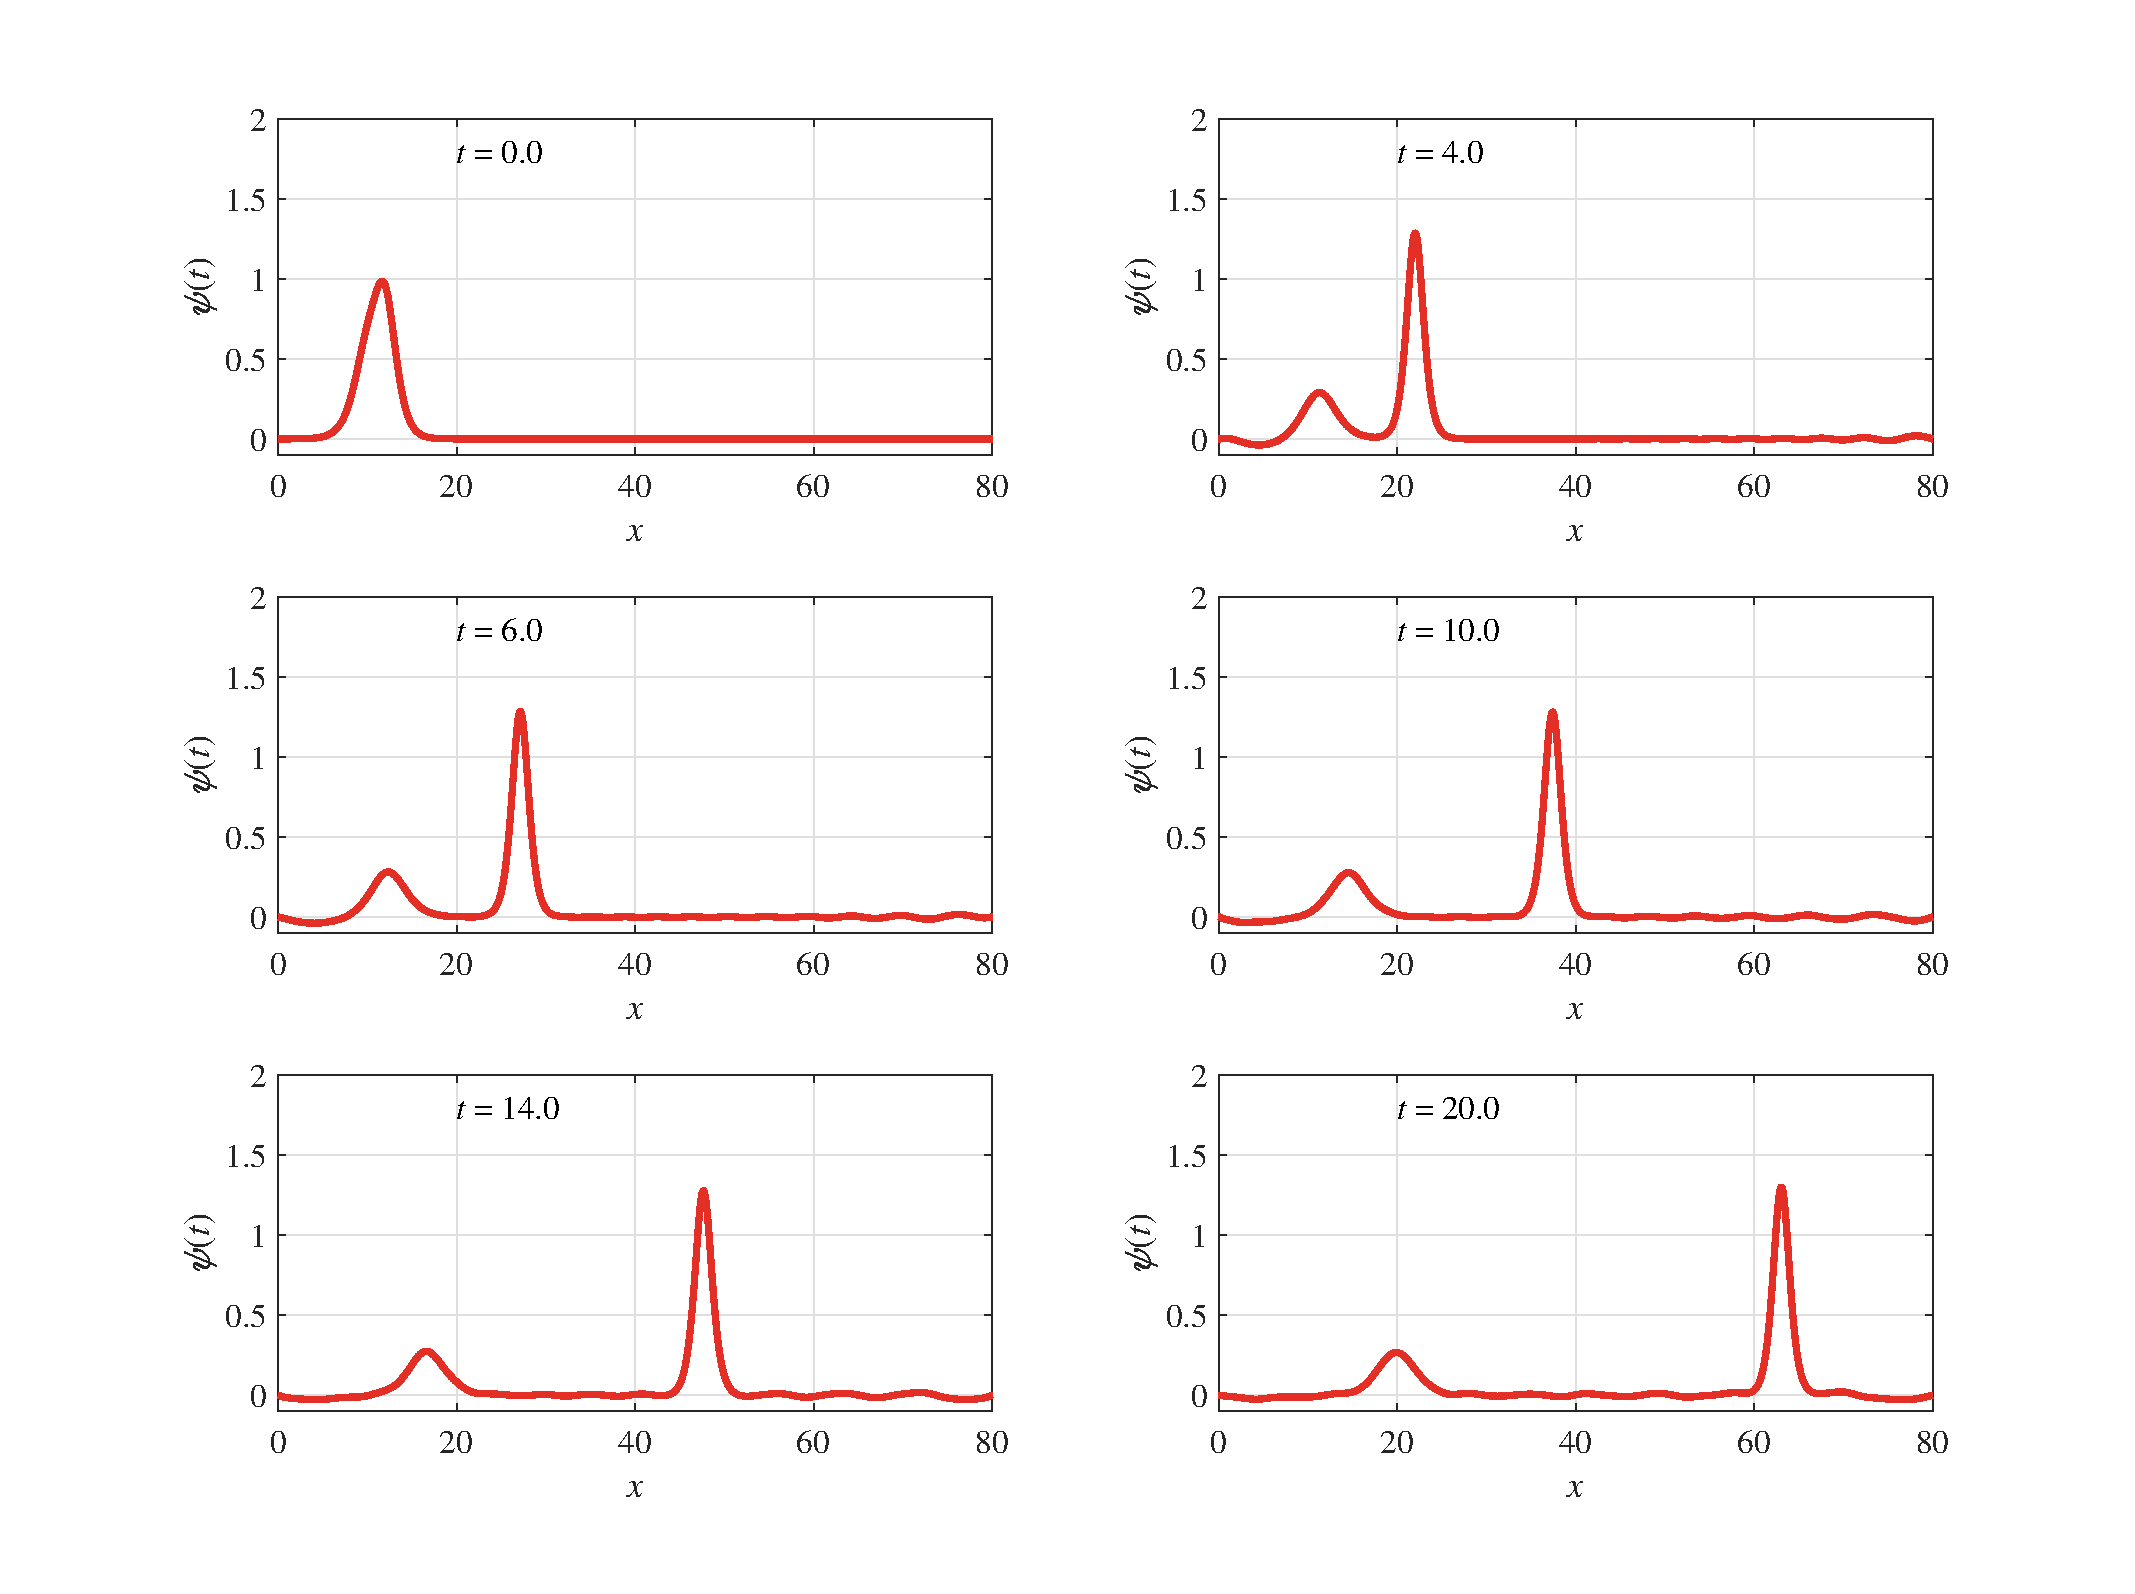
\includegraphics[width=\textwidth]{KdVSolitonSumme1.pdf}
    \caption[Ausbreitung einer Summe aus einzelnen, aber �bereinander liegenden
    Soliton-L�sungen der Korteweg-de-Vries-Gleichung.]
    {Ausbreitung einer Summe aus einzelnen, aber �bereinander liegenden
      Soliton-L�sungen der Korteweg-de-Vries-Gleichung. Die Ausrbreitung
      erfolgt mit unerwarteten Geschwindigkeiten und es sind Deformationionen
      zu erkennen.}
    \label{abb:kontmech_KdVSolitonSumme1}
  \end{figure}

  Diese Summe verh�lt sich ungew�hnlich. Man erkennt zwar nach einiger Zeit,
  dass sich zwei einzelne Soliton-L�sungen zu trennen scheinen, diese breiten
  sich aber nicht mit den Geschwindigkeiten $c=1$ und $c=1.5$ aus, die
  f�r die urspr�ngliche Summe angesetzt waren. Zus�ztlich scheinen
  wellenf�rmige St�rungen mit kleiner Amplitude aufzutreten. Tats�chlich
  scheint die Propagation in der KdV-Gleichung zu sehr vielen soliton-�hnlichen
  Erhebungen zu f�hren, die sich alle mit unterschiedlicher Geschwindigkeit
  ausbreiten. Zus�tzliche St�rungen enstehen hier, da diese St�rungen an den
  R�ndern des endlichen Gitters reflektiert werden, was ein Artefakt der
  numerischen L�sung ist.

  Eine Summe aus zwei Soliton-L�sungen kann allerdings auch eine gute
  N�herung einer exakten L�sung der Korteweg-de-Vries-Gleichung sein. Das
  ist dann der Fall, wenn sich die beiden Solitonen kaum �berschneiden. Dies
  kann man bereits an den Gleichungen \eqref{eq:kontmech_KdVSumme1} bzw.
  \eqref{eq:kontmech_KdVSumme2} erkennen. Ist immer eine der Wellenfunktionen
  und ihre erste $x$-Ableitung Null, so verschwindet auch der st�rende Term.
  In der numerischen L�sung dr�ckt sich das darin aus, dass beide Solitonen
  aus der Summe so in der KdV-Gleichung propagieren, wie man es von ihnen
  erwartet. 

  \begin{figure}
    \centering
    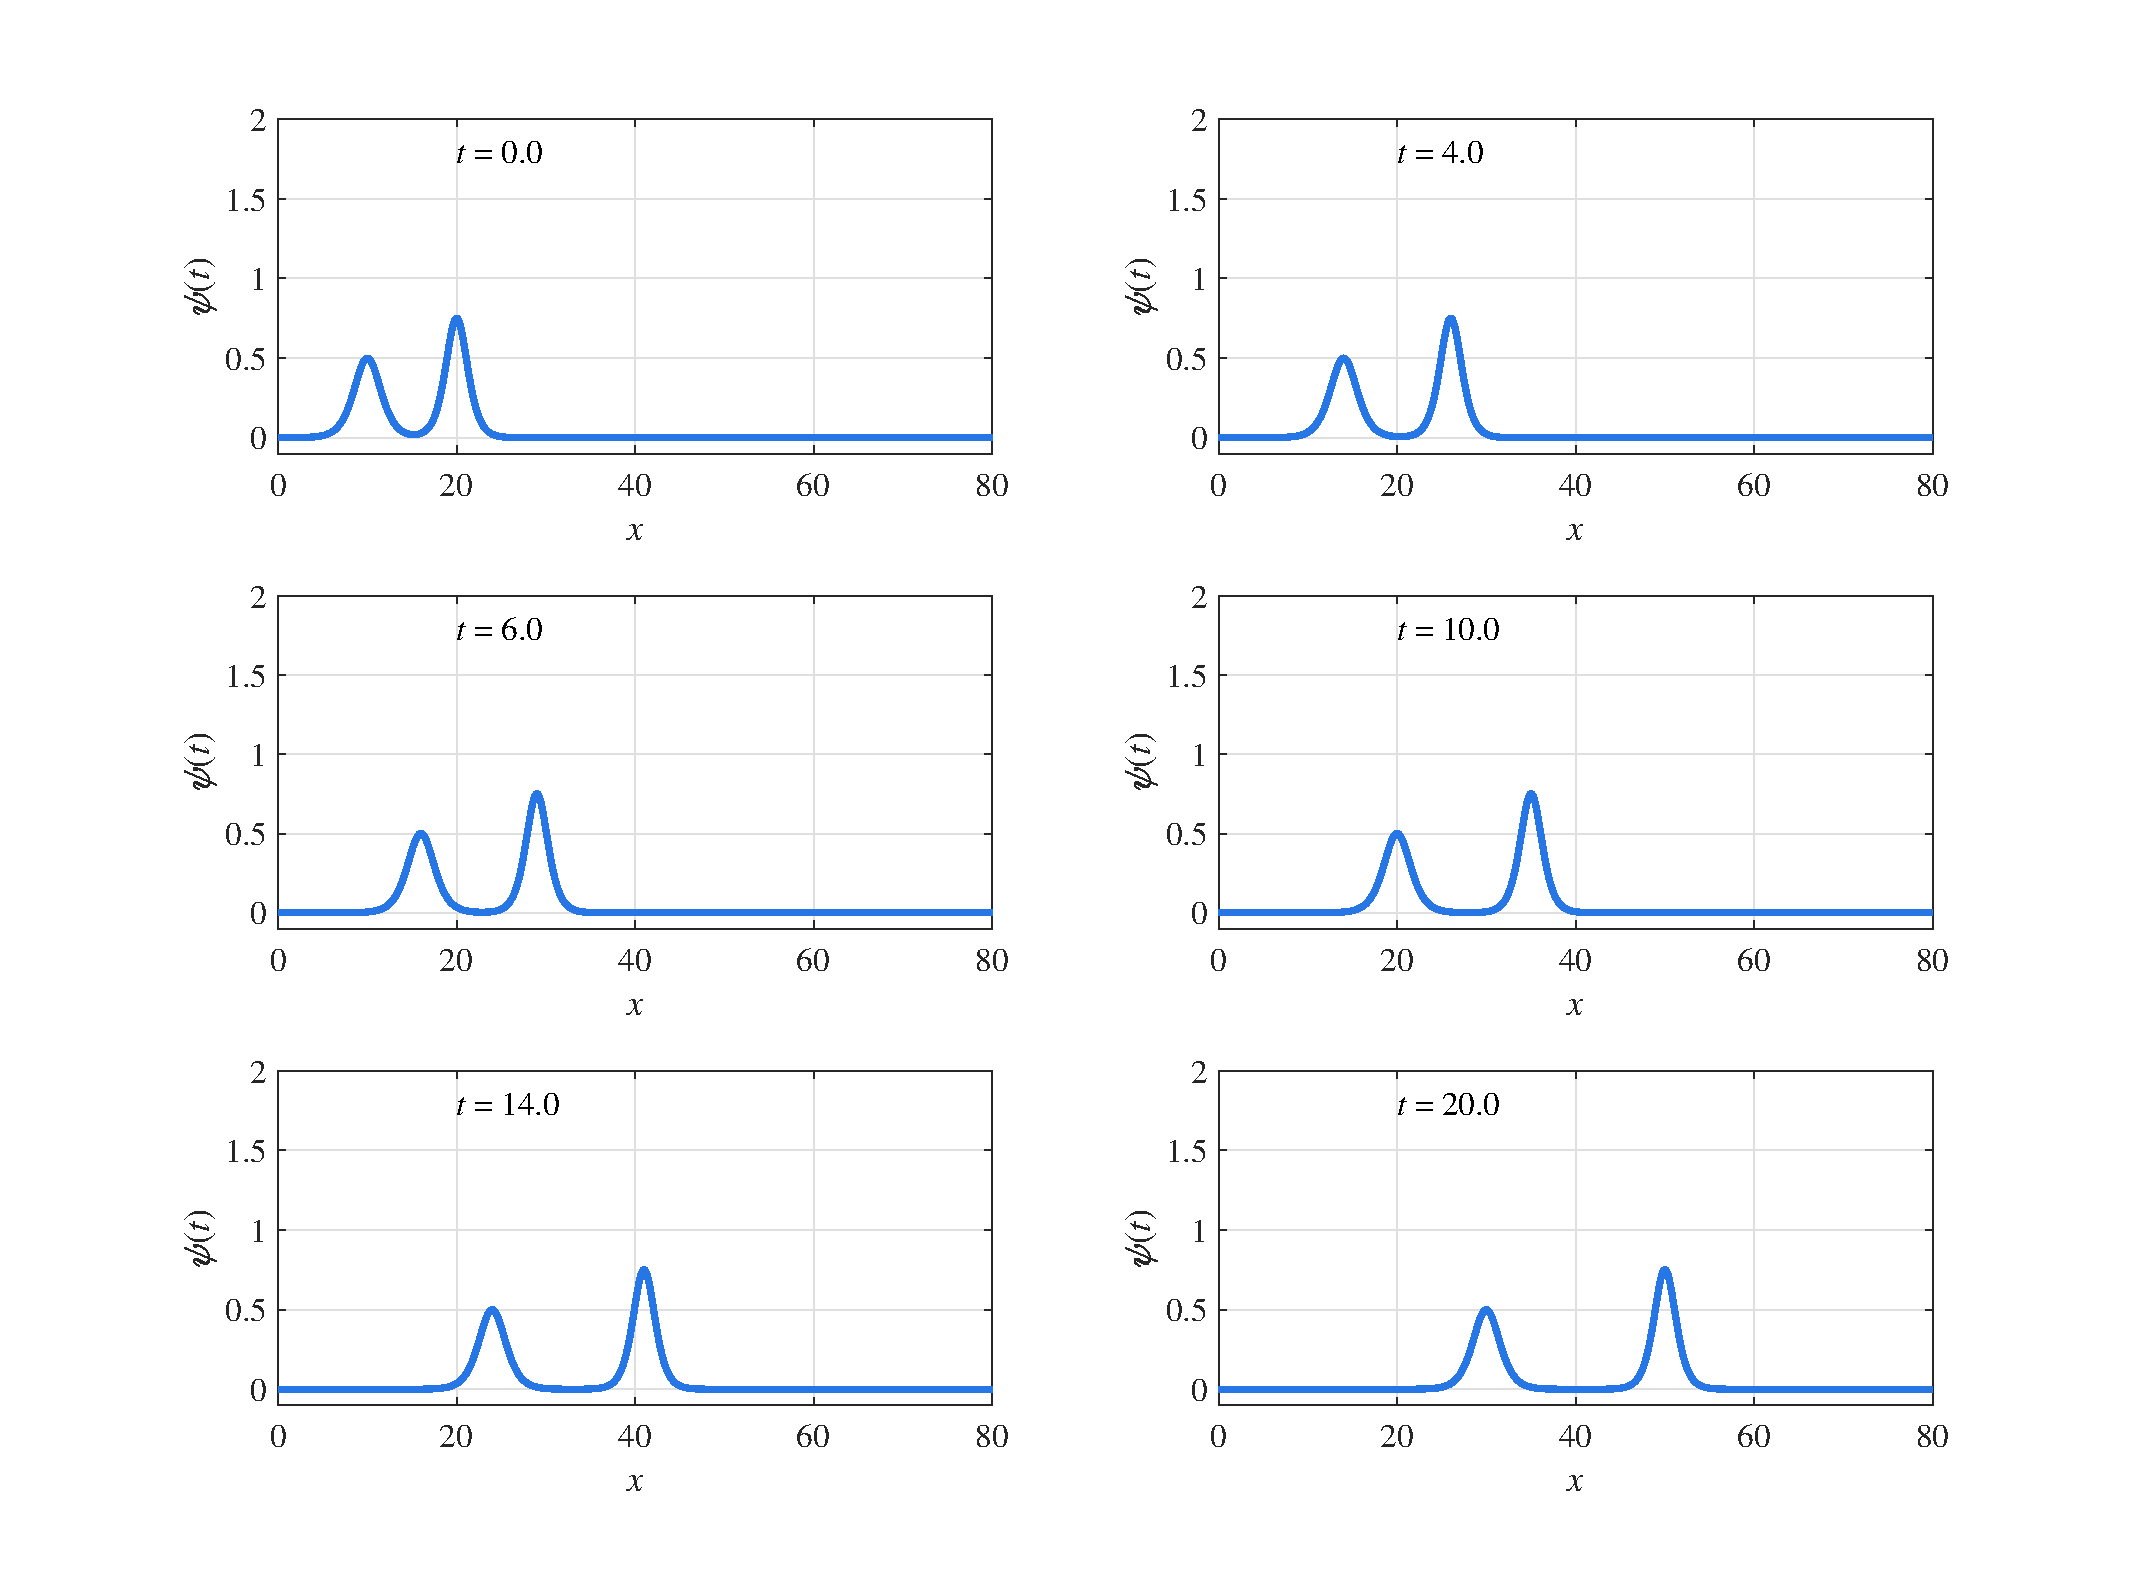
\includegraphics[width=\textwidth]{KdVSolitonSumme2.pdf}
    \caption[Ausbreitung einer Summe aus einzelnen, nicht �bereinander liegenden
    Soliton-L�sungen der Korteweg-de-Vries-Gleichung.]
    {Ausbreitung einer Summe aus einzelnen, nicht �bereinander liegenden
      Soliton-L�sungen der Korteweg-de-Vries-Gleichung. Die Ausbreitung ist
      in der graphischen Darstellung nicht von der von zwei einzelnen Solitonen
      zu unterscheiden.}
    \label{abb:kontmech_KdVSolitonSumme2}
  \end{figure}

  Als Beispiel ist in \figref{kontmech_KdVSolitonSumme2} eine solche Summe
  dargestellt.  Die Anfangsbedingung enth�lt erneut eine Summe aus zwei
  Solitonen mit den Geshwindigkeitsparametern $c=1$ und $c=1.5$. Dabei wurde
  in der Summe das zweite Soliton mit $c=1.5$ deutlich rechts vom ersten
  angesetzt. Zum Beginn der Propagation tritt es erst dort auf, wo das erste
  schon (numerisch) auf Null abgefallen ist. Tatschlich ergibt sich eine
  Propagation, wie wir sie f�r zwei getrennte Soliton-L�sungen mit genau diesen
  Geschwindigkeiten erwarten.

\item Um die Interaktion von zwei Solitonen zu betrachten, l�sen wir wieder
  die Korteweg-de-Vries-Gleichung mit einer Einfangsbedingung, die zwei
  r�umlich getrennte Solitonen enth�lt. Eine solche Situation wird mit einem
  Programm aus der \matlab{}-Datei \mlkontmechref{KdV04.m} gel�st. Das
  Ergebnis ist in \figref{kontmech_KdVSolitonInteraktion} dargestellt. Die
  Anfangsbedingung zur Zeit $t=0$ enth�lt eine �berlagerung aus zwei nach
  rechts laufenden Solitonen mit den Geschwindigkeitsparamtern $c=1$ und
  $c=2$, wobei das schnellere Soliton links vom langsameren ist (dicke
  blaue Linien). Im Zeitverlauf "`�berholt"' es das langsamere Soliton und es
  kommt zur Interaktion. Anschlie�end trennen sie sich wieder und beide
  Solitonen bewegen sich fast so fort, wie sie es ohne Interaktion getan
  h�tten. Einziger Unterschied ist eine Phasenverschiebung $\Delta x$, also
  eine Verschiebung gegen�ber der erwarteten Position ohne Interaktion.

  \begin{figure}
    \centering
    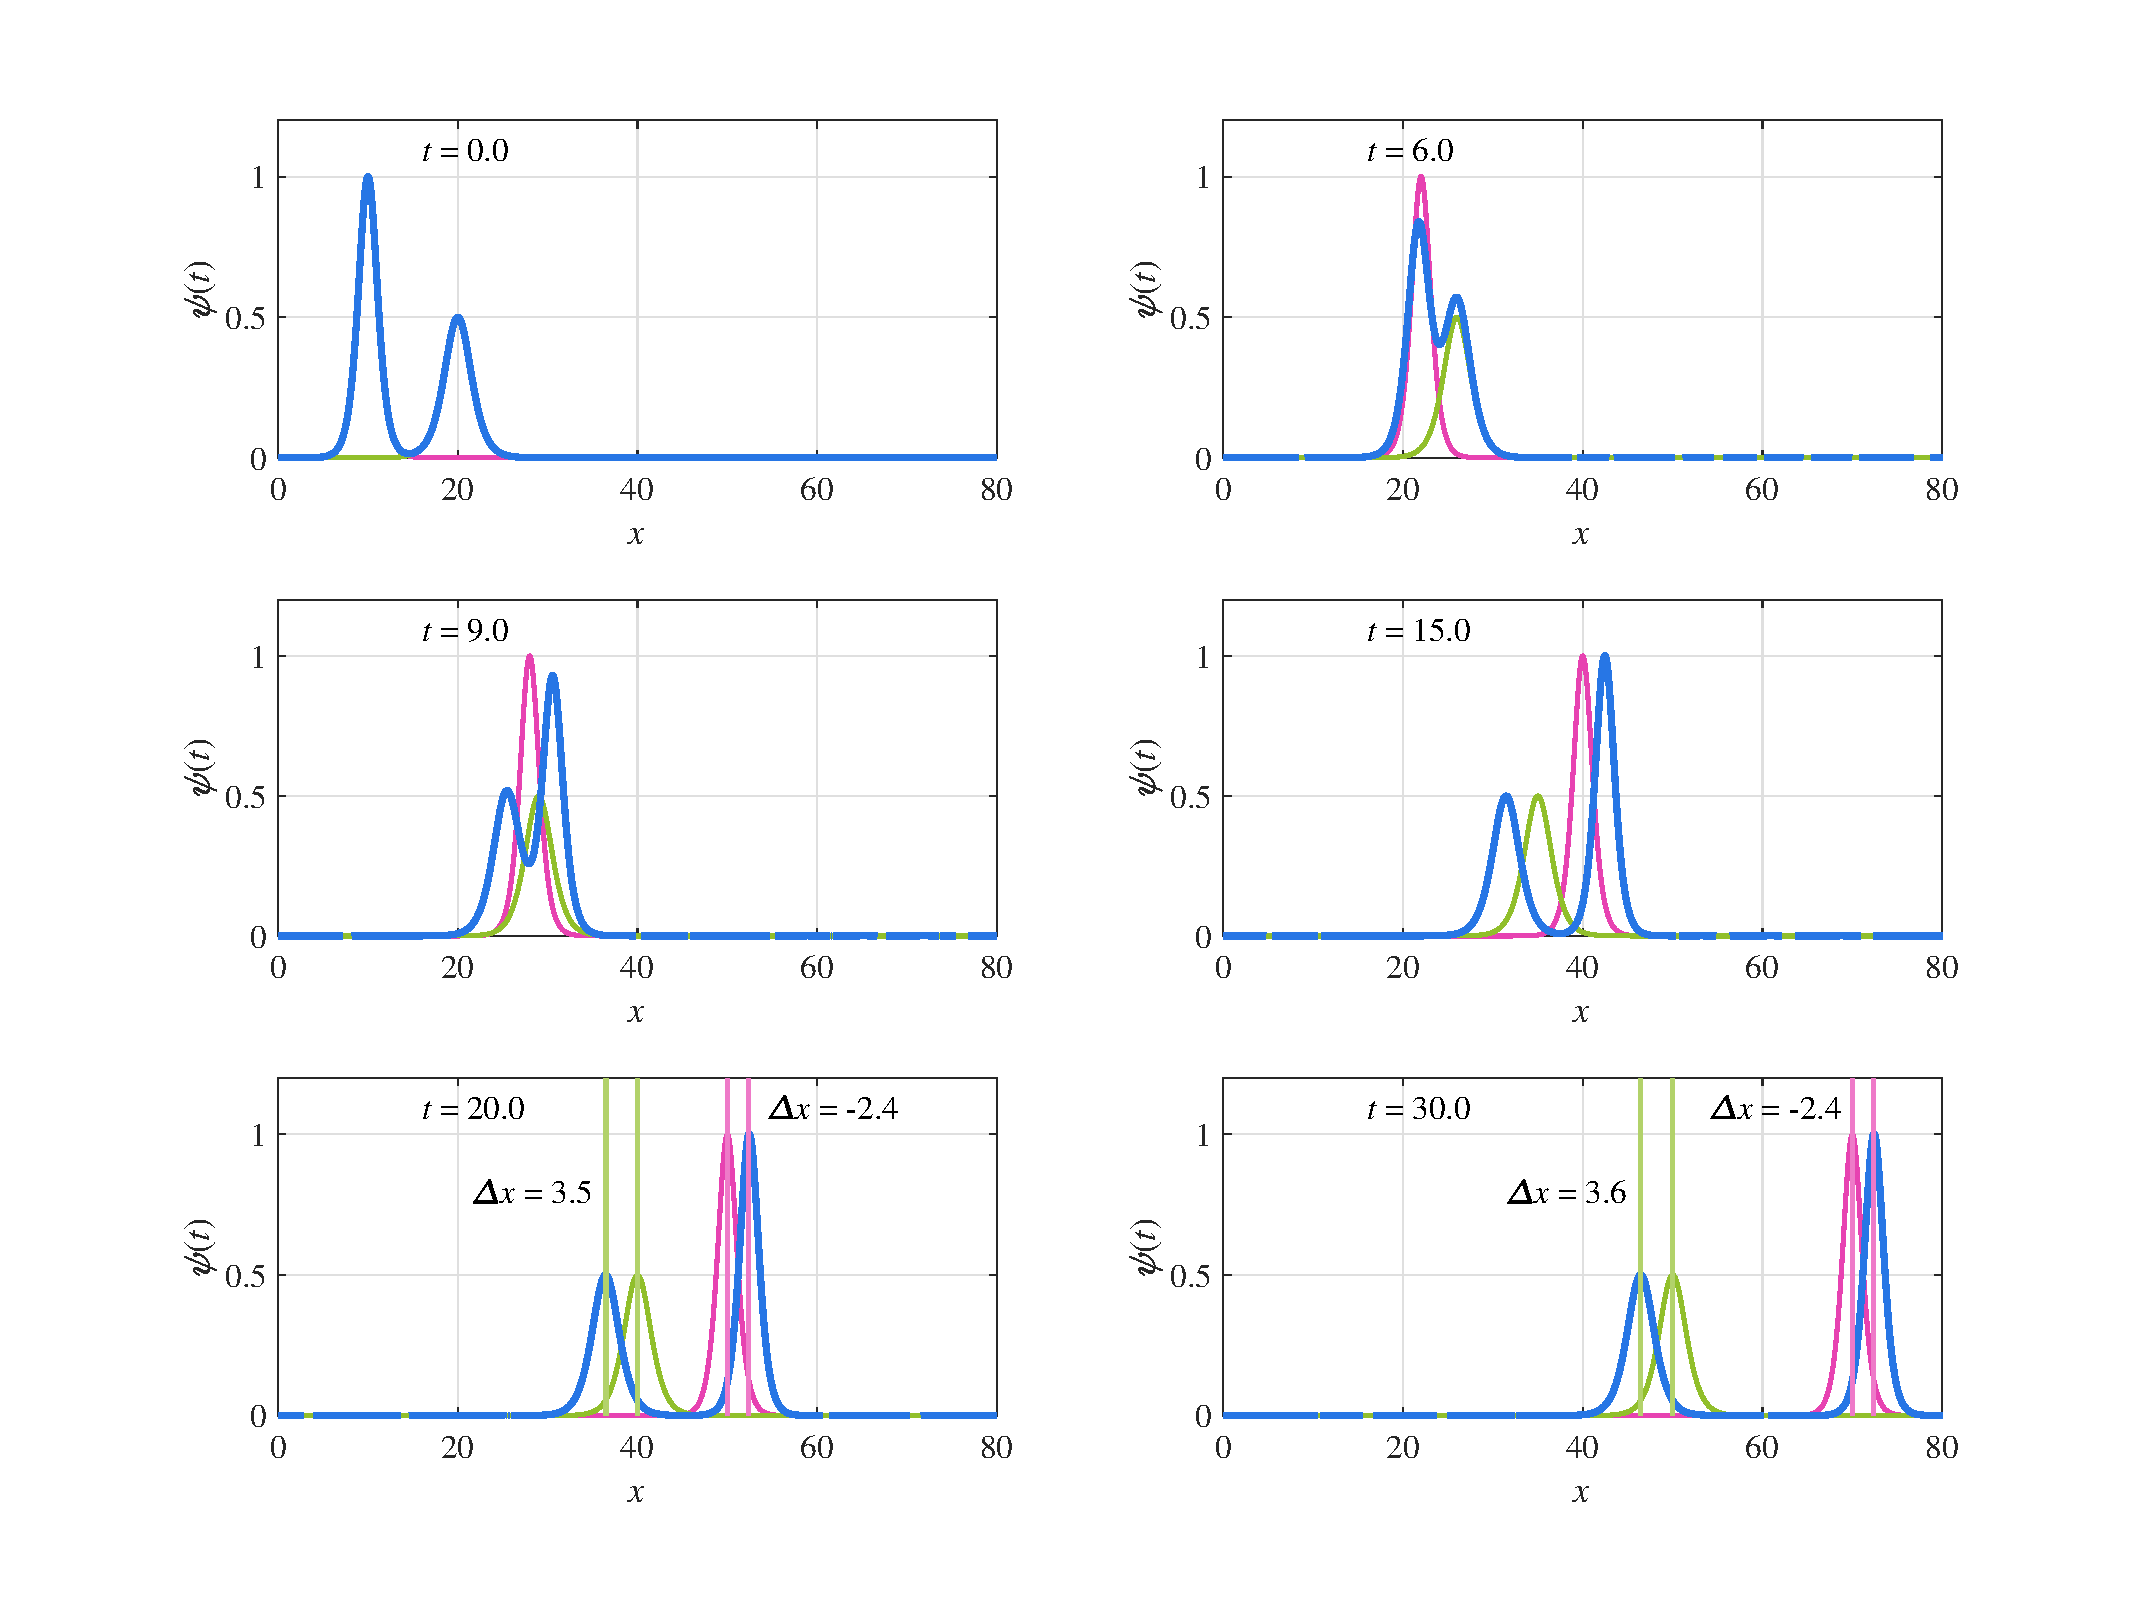
\includegraphics[width=\textwidth]{KdVSolitonInteraktion.pdf}
    \caption[Interaktion zwischen zwei Solitonen der
    Korteweg-de-Vries-Gleichung.]{Nach der Interaktion zwischen zwei Solitonen
      der Korteweg-de-Vries-Gleichung (dicke blaue Linien) ergibt sich eine
      Phasenverschiebung $\Delta x$ geben�ber einzelnen Soliton-L�sungen, die
      sich ungest�rt ausbreiten (d�nne Linien).}
    \label{abb:kontmech_KdVSolitonInteraktion}
  \end{figure}
  
  Um diese Phasenverschiebung bestimmen zu k�nnen, tragen wir ebenfalls die
  analytischen L�sungen f�r zwei einzelne Solitionen auf (d�nne Linien, gr�n
  zu $c=1$, magenta zu $c=2$), die zu $t=0$ mit  der blauen Linie
  �bereinstimmen. Bereits w�hrend der Interaktion sieht man Unterschiede,
  die sich nach der Interaktion zu einem festen Abstand zwischen ungest�rter
  L�sung und L�sung mit Interaktion ergeben. Diese Abst�nde lassen sich durch
  Ausmessen des Abstands bestimmen. Dies geschieht im Programm, indem die
  Position der Maxima der numerischen L�sung ermittelt wird. Ihre Differenz
  zu erwarteten Position der analytischen L�sung
  \begin{equation}
    \Delta x = x_\text{analytisch} - x_\text{numerisch mit Interaktion}
  \end{equation}
  l�sst sich daraus berechnen. Dies geschieht f�r zwei verschiedene Zeiten
  $t$ und man findet:\\

  \begin{tabular}{lll}
    Zeit & Soliton mit $c=1$ & Soliton mit $c=2$ \\
    \hline
    $t=20$ & $\Delta x = 3.5$ & $\Delta x = -2.4$ \\
    $t=30$ & $\Delta x = 3.6$ & $\Delta x = -2.4$ \\
  \end{tabular}\\

  Dies entspricht einem konstanten Abstand nach der Interaktion. Die kleine
  Abweichung f�r das $c=1$-Soliton l�sst sich mit der numerischen Aufl�sung
  erkl�ren. In der numerischen Rechnung haben zwei Gitterpunkte gerade den
  Abstand $0.1$.
\end{enumerate}

\end{sol} 
\textcolor{blue} {$\rightarrow$ zur} \probref{kontmech_soliton1}.\\
\noindent\rule[1ex]{\textwidth}{0.5pt}  \newpage  \clearpage

%-----------------------------------------------------------------------------------------------------------

\begin{sol}{prob:kontmech_soliton2}\label{lsg:kontmech_soliton2} %�bung27
\textbf{Solitonen II}\\ \\

Wir gehen sowohl analytische als auch numerische L�sungen der Solitonen-Typen
beider Gleichungen durch. Um die �bersichtlichkeit zu wahren gehen wir zun�chst
auf die L�sungen der Sinus-Gordon-Gleichung und danach auf die der nichtlinearen
Schr�dingergleichung ein. Am Ende folgt ein Vergleich der Solitonen beider
Gleichungen.

Zun�chst wollen wir die analtyisch gegebenen Solitonen 
\begin{equation}
  \psi(x,t) = 4 \arctan \lk \mathrm{exp}\lek \pm \frac{x-vt}{\sqrt{1-(v/c)^2}}
  \rek \rk
  \tag{\ref{eq:kontmech_soliton04}}
\end{equation}
f�r verschiedene Parameter darstellen. Diese sind in
\figref{kontmech_SinusGordon1} gegeben.

\begin{figure}
  \centering
  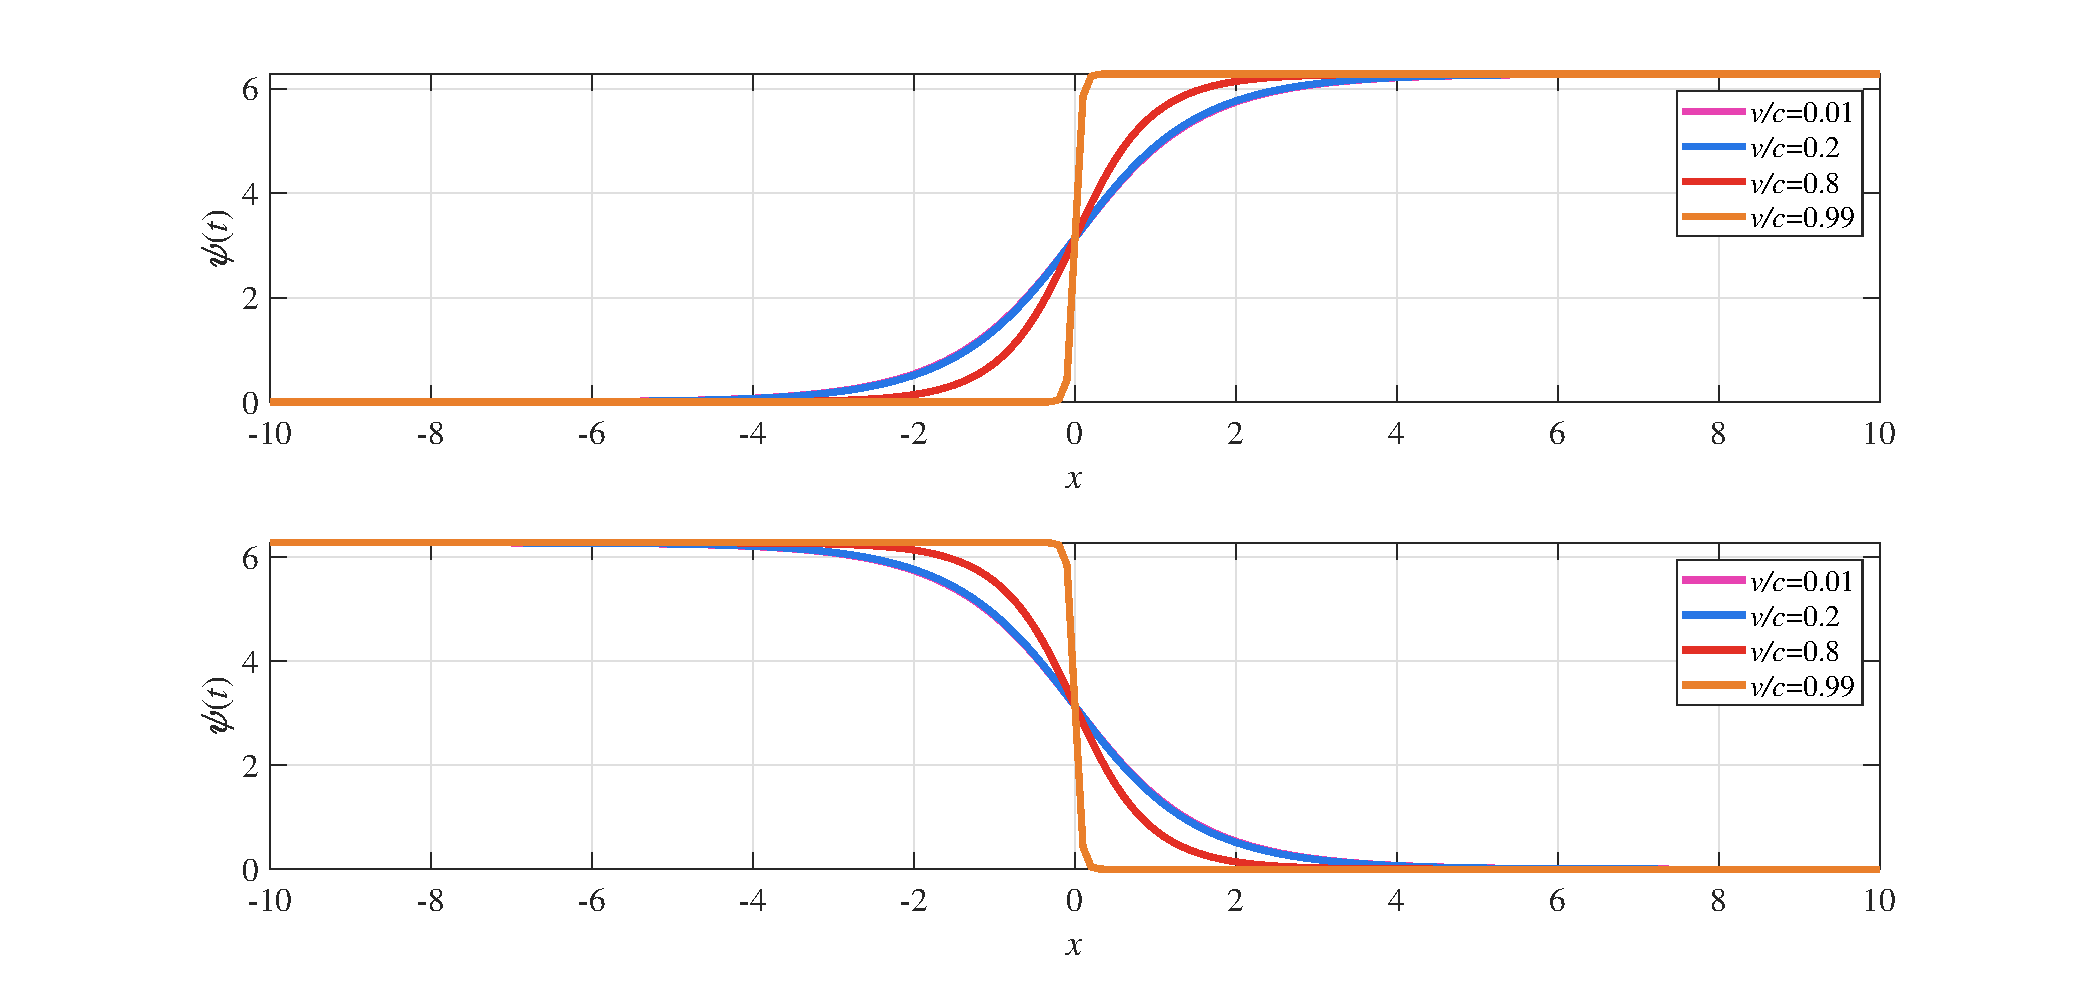
\includegraphics[width=\textwidth]{SinusGordon1.pdf}
  \caption[L�sungen der Sinus-Gordon-Gleichung bei Variation der
  Parameter]{L�sungen der Sinus-Gordon-Gleichung bei Variation der
    Parameter, wobei ausschlie�lich das Verh�ltnis $v/c$ ausschlaggebend ist.}
  \label{abb:kontmech_SinusGordon1}
\end{figure}

Die Form h�ngt dabei nur vom Verh�ltnis $v/c$ ab, da die Geschwindigkeit $v$
allein ausschlie�lich einen Einfluss auf die Fortbewegung des Solitons hat.
Sie besteht aus einer ansteigenden Stufe f�r den ersten Typ mit dem Vorzeichen
$+$ im Exponenten (kink) bzw. einer absteigenden Stufe f�r das Vorzeichen $-$
(anti-kink). Je gr��er das Verh�ltnis ist, desto steiler steigt die Stufe an
bzw. desto steiler f�llt sie ab.

Die Fortbewegung ist in \figref{kontmech_SinusGordon2} dargestellt. Die Form
bleibt bei der Propagation erhalten und es gibt eine exakte �bereinstimmung
der numerischen L�sung der partiellen Differentialgleichung mit der
Methode der finiten Differenzen (dick gestrichelte Linien) mit der analytischen
L�sung (d�nne durchgezogene Linien). Dies zeigt, dass hier tats�chlich
Solitonen vorliegen, die mit unver�nderter Form nach rechts propagieren.

\begin{figure}
  \centering
  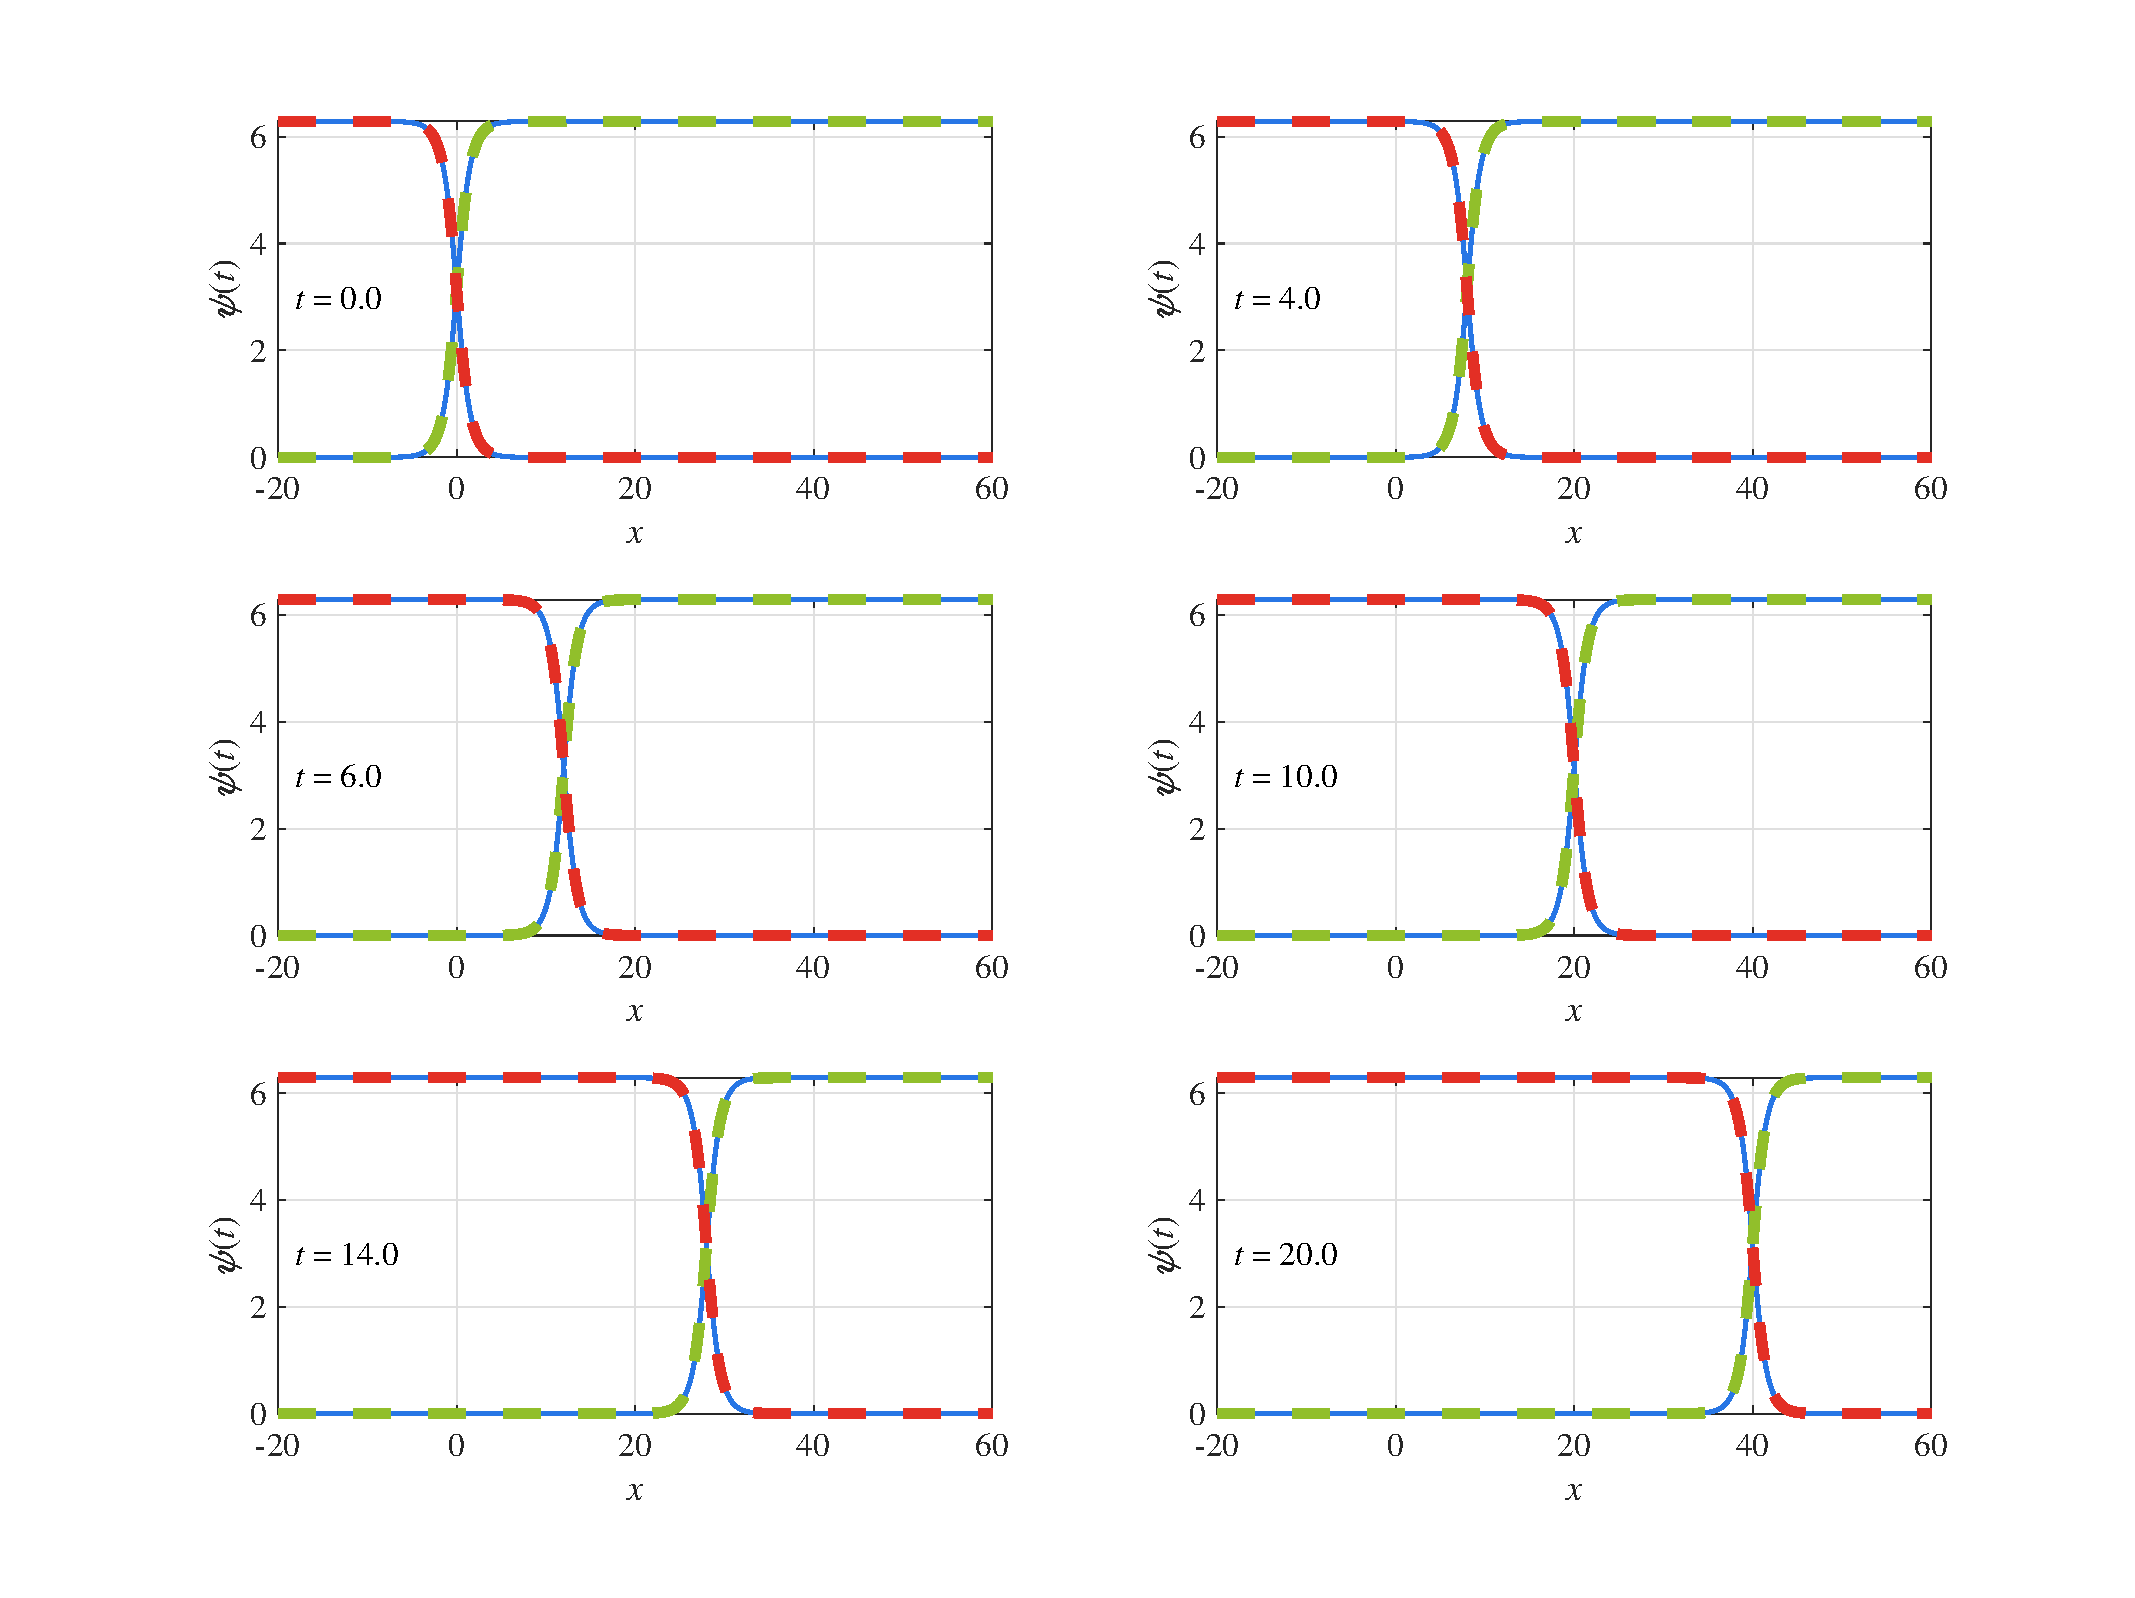
\includegraphics[width=\textwidth]{SinusGordon2.pdf}
  \caption[Numerische L�sungen der Sinus-Gordon-Gleichung]{Numerische
    L�sungen der Sinus-Gordon-Gleichung mit einer Geschwindigkeit $v = 2$
    bei einer Maximalgeschwindigkeit von $c = 10$. Die numerische Intergration
    mit der Methode der finiten Differenzen (dick gestrichelte Linien) stimmt
    exakt mit der analytischen Form (d�nne durchgezogene Linien) �berein.}
  \label{abb:kontmech_SinusGordon2}
\end{figure}

Es l�sst sich selbstverst�ndlich auch analytisch zeigen, dass die Funktionen
\eqref{eq:kontmech_soliton04} L�sungen der Sinus-Gordon-Gleichung
\begin{equation}
  \frac{1}{c^2}\frac{\partial^2 \psi}{\partial t^2}
  - \frac{\partial^2 \psi}{\partial x^2}  + \sin \psi = 0
  \tag{\ref{eq:kontmech_soliton03}}
\end{equation}
sind. Dazu berechnen wir zun�chst die ben�tigten Ableitungen. Diese sind
\begin{subequations}
  \allowdisplaybreaks
  \begin{align}
    \frac{\partial \psi}{\partial t}
    &= \frac{\mp 4\, v}{\sqrt{1-(v/c)^2}}
      \frac{\exp \lek \pm \frac{x-vt}{\sqrt{1-(v/c)^2}} \rek}
      {1+\exp \lek \pm 2\, \frac{x-vt}{\sqrt{1-(v/c)^2}} \rek} \; , \\
    \frac{\partial^2 \psi}{\partial t^2}
    &= \frac{4\, v^2}{1-(v/c)^2}
      \frac{\exp \lek \pm \frac{x-vt}{\sqrt{1-(v/c)^2}} \rek}
      {1+\exp \lek \pm 2\, \frac{x-vt}{\sqrt{1-(v/c)^2}} \rek} \lk 1 -
      \frac{2 \exp \lek \pm 2\, \frac{x-vt}{\sqrt{1-(v/c)^2}} \rek}
      {1+\exp \lek \pm 2\, \frac{x-vt}{\sqrt{1-(v/c)^2}} \rek} \rk  \notag \\
    &= \frac{4\, v^2}{1-(v/c)^2}
      \frac{\exp \lek \pm \frac{x-vt}{\sqrt{1-(v/c)^2}} \rek}
      {1+\exp \lek \pm 2\, \frac{x-vt}{\sqrt{1-(v/c)^2}} \rek} 
      \frac{1- \exp \lek \pm 2\, \frac{x-vt}{\sqrt{1-(v/c)^2}} \rek}
      {1+\exp \lek \pm 2\, \frac{x-vt}{\sqrt{1-(v/c)^2}} \rek} \notag \\
    &= \frac{4\, v^2}{1-(v/c)^2}
      \frac{\exp \lek \pm \frac{x-vt}{\sqrt{1-(v/c)^2}} \rek -
      \exp \lek \pm 3\, \frac{x-vt}{\sqrt{1-(v/c)^2}} \rek}
      {\lk 1+\exp \lek \pm 2\, \frac{x-vt}{\sqrt{1-(v/c)^2}} \rek \rk^2} \; , \\
    \frac{\partial \psi}{\partial x} 
    &= \frac{\pm 4}{\sqrt{1-(v/c)^2}}
      \frac{\exp \lek \pm \frac{x-vt}{\sqrt{1-(v/c)^2}} \rek}
      {1+\exp \lek \pm 2\, \frac{x-vt}{\sqrt{1-(v/c)^2}} \rek} \; , \\
    \frac{\partial^2 \psi}{\partial x^2}
    &= \frac{4}{1-(v/c)^2}
      \frac{\exp \lek \pm \frac{x-vt}{\sqrt{1-(v/c)^2}} \rek -
      \exp \lek \pm 3\, \frac{x-vt}{\sqrt{1-(v/c)^2}} \rek}
      {\lk 1+\exp \lek \pm 2\, \frac{x-vt}{\sqrt{1-(v/c)^2}} \rek \rk^2} \; .
  \end{align}
\end{subequations}
F�r die Sinusfunktion in der Differentialgleichung verwenden wir die
Additionstheoreme
\begin{equation*}
  \sin x = \frac{2\tan(x/2)}{1+\tan^2(x/2)} \qquad \text{sowie}
  \qquad \tan x = \frac{2\tan(x/2)}{1-\tan^2(x/2)} 
\end{equation*}
und setzen sie ineinander ein
\begin{equation*}
  \sin x = \frac{2 \frac{2\tan(x/4)}{1-\tan^2(x/4)} }{1 +
    \lk \frac{2\tan(x/4)}{1-\tan^2(x/4)} \rk^2}
  = 4 \, \frac{\tan(x/4) - \tan^3(x/4)}{\lk 1 + \tan^2(x/4) \rk^2} \; .
\end{equation*}
Damit erhalten wir
\begin{multline*}
  \frac{1}{c^2}\frac{\partial^2 \psi}{\partial t^2}
  - \frac{\partial^2 \psi}{\partial x^2}  + \sin \psi
  = \frac{1}{c^2} \frac{4\, v^2}{1-(v/c)^2}
      \frac{\exp \lek \pm \frac{x-vt}{\sqrt{1-(v/c)^2}} \rek -
      \exp \lek \pm 3\, \frac{x-vt}{\sqrt{1-(v/c)^2}} \rek}
    {\lk 1+\exp \lek \pm 2\, \frac{x-vt}{\sqrt{1-(v/c)^2}} \rek \rk^2} \\
    - \frac{4}{1-(v/c)^2}
      \frac{\exp \lek \pm \frac{x-vt}{\sqrt{1-(v/c)^2}} \rek -
      \exp \lek \pm 3\, \frac{x-vt}{\sqrt{1-(v/c)^2}} \rek}
    {\lk 1+\exp \lek \pm 2\, \frac{x-vt}{\sqrt{1-(v/c)^2}} \rek \rk^2}
    + 4\, \frac{\tan(\psi/4) - \tan^3(\psi/4)}{\lk 1 + \tan^2(\psi/4) \rk^2} \\
    = - 4 \frac{\exp \lek \pm \frac{x-vt}{\sqrt{1-(v/c)^2}} \rek -
      \exp \lek \pm 3\, \frac{x-vt}{\sqrt{1-(v/c)^2}} \rek}
    {\lk 1+\exp \lek \pm 2\, \frac{x-vt}{\sqrt{1-(v/c)^2}} \rek \rk^2}
    + 4\, \frac{\exp \lek \pm \frac{x-vt}{\sqrt{1-(v/c)^2}} \rek
      - \exp \lek \pm 3\, \frac{x-vt}{\sqrt{1-(v/c)^2}} \rek}
    {\lk 1 + \exp \lek \pm 2\, \frac{x-vt}{\sqrt{1-(v/c)^2}} \rek \rk^2}
    = 0 \; ,
\end{multline*}
was best�tigt, dass die Differentialgleichung von der Funktion
\eqref{eq:kontmech_soliton04} erf�llt wird. Somit haben wir gezeigt, dass
tats�chlich analytisch bekannte Solitonen der Sinus-Gordon-Gleichung
vorliegen.

F�r eine numerische L�sung der partiellen Differentialgleichung mit der
Methode der finiten Differenzen geben wir zun�chst wieder die diskretisierten
Ableitungen an. Wir ben�tigen f�r die Sinus-Gordon-Gleichung
\eqref{eq:kontmech_soliton03} die zweiten Ableitungen nach der Zeit und dem
Ort,
\begin{subequations}
  \begin{align}
    \frac{\partial^2 \psi(x_i,t_j)}{\partial t^2}
    &= \frac{\psi(x_{i},t_{j+1}) + \psi(x_{i},t_{j-1}) -2 \psi(x_{i},t_{j})}
      {\Delta t^2}  \; , \\
    \frac{\partial^2 \psi(x,t)}{\partial x^2}
    &= \frac{\psi(x_{i+1},t_{j}) + \psi(x_{i-1},t_{j}) -2 \psi(x_{i},t_{j})}
      {\Delta x^2}  \; .
  \end{align}
\end{subequations}
Mit diesen l�sst sich die Sinus-Gordon-Gleichung diskret schreiben als
\begin{subequations}
  \begin{multline}
    \frac{1}{c^2} \frac{\psi(x_{i},t_{j+1}) + \psi(x_{i},t_{j-1})
      -2 \psi(x_{i},t_{j})}{\Delta t^2}
    - \frac{\psi(x_{i+1},t_{j}) + \psi(x_{i-1},t_{j}) -2 \psi(x_{i},t_{j})}
    {\Delta x^2} \\
    + \sin\psi\lk \psi(x_{i},t_{j}) \rk = 0 \; ,
  \end{multline}
  was sich zum Interrationsschritt
  \begin{multline}
    \psi(x_{i},t_{j+1}) = 2 \psi(x_{i},t_{j}) - \psi(x_{i},t_{j-1})
    + c^2 \frac{\Delta t^2}{\Delta x^2} \left ( \psi(x_{i+1},t_{j})
      + \psi(x_{i-1},t_{j}) -2 \psi(x_{i},t_{j}) \right ) \\
    - c^2 \, \Delta t^2\, \sin\lk \psi(x_{i},t_{j}) \rk 
  \end{multline}
\end{subequations}
f�r die Methode der finiten Differenzen aufl�sen l�sst.
Diese Berechnung wird in einem Programm in der \matlab{}-Datei
\mlkontmechref{SinusGordonSolitonen.m} durchgef�hrt.


Vollkommen analog gehen wir f�r die nichtlineare Schr�dinger-Gleichung vor.
zun�chst stellen wir die Fundamentall�sung
\begin{align}
  \psi(x,t) = A_0\;\sech \lk \frac{t- x/v }{\tau_0} \rk \mathrm{exp}\lek
  -\im \frac{x}{x_0} \rek
  \tag{\ref{eq:kontmech_soliton06}}
\end{align}
f�r verschiedene Parameter $v$ und $g$ dar. Die L�sungen k�nnen in
\figref{kontmech_NLSG1} gefunden werden.

\begin{figure}
  \centering
  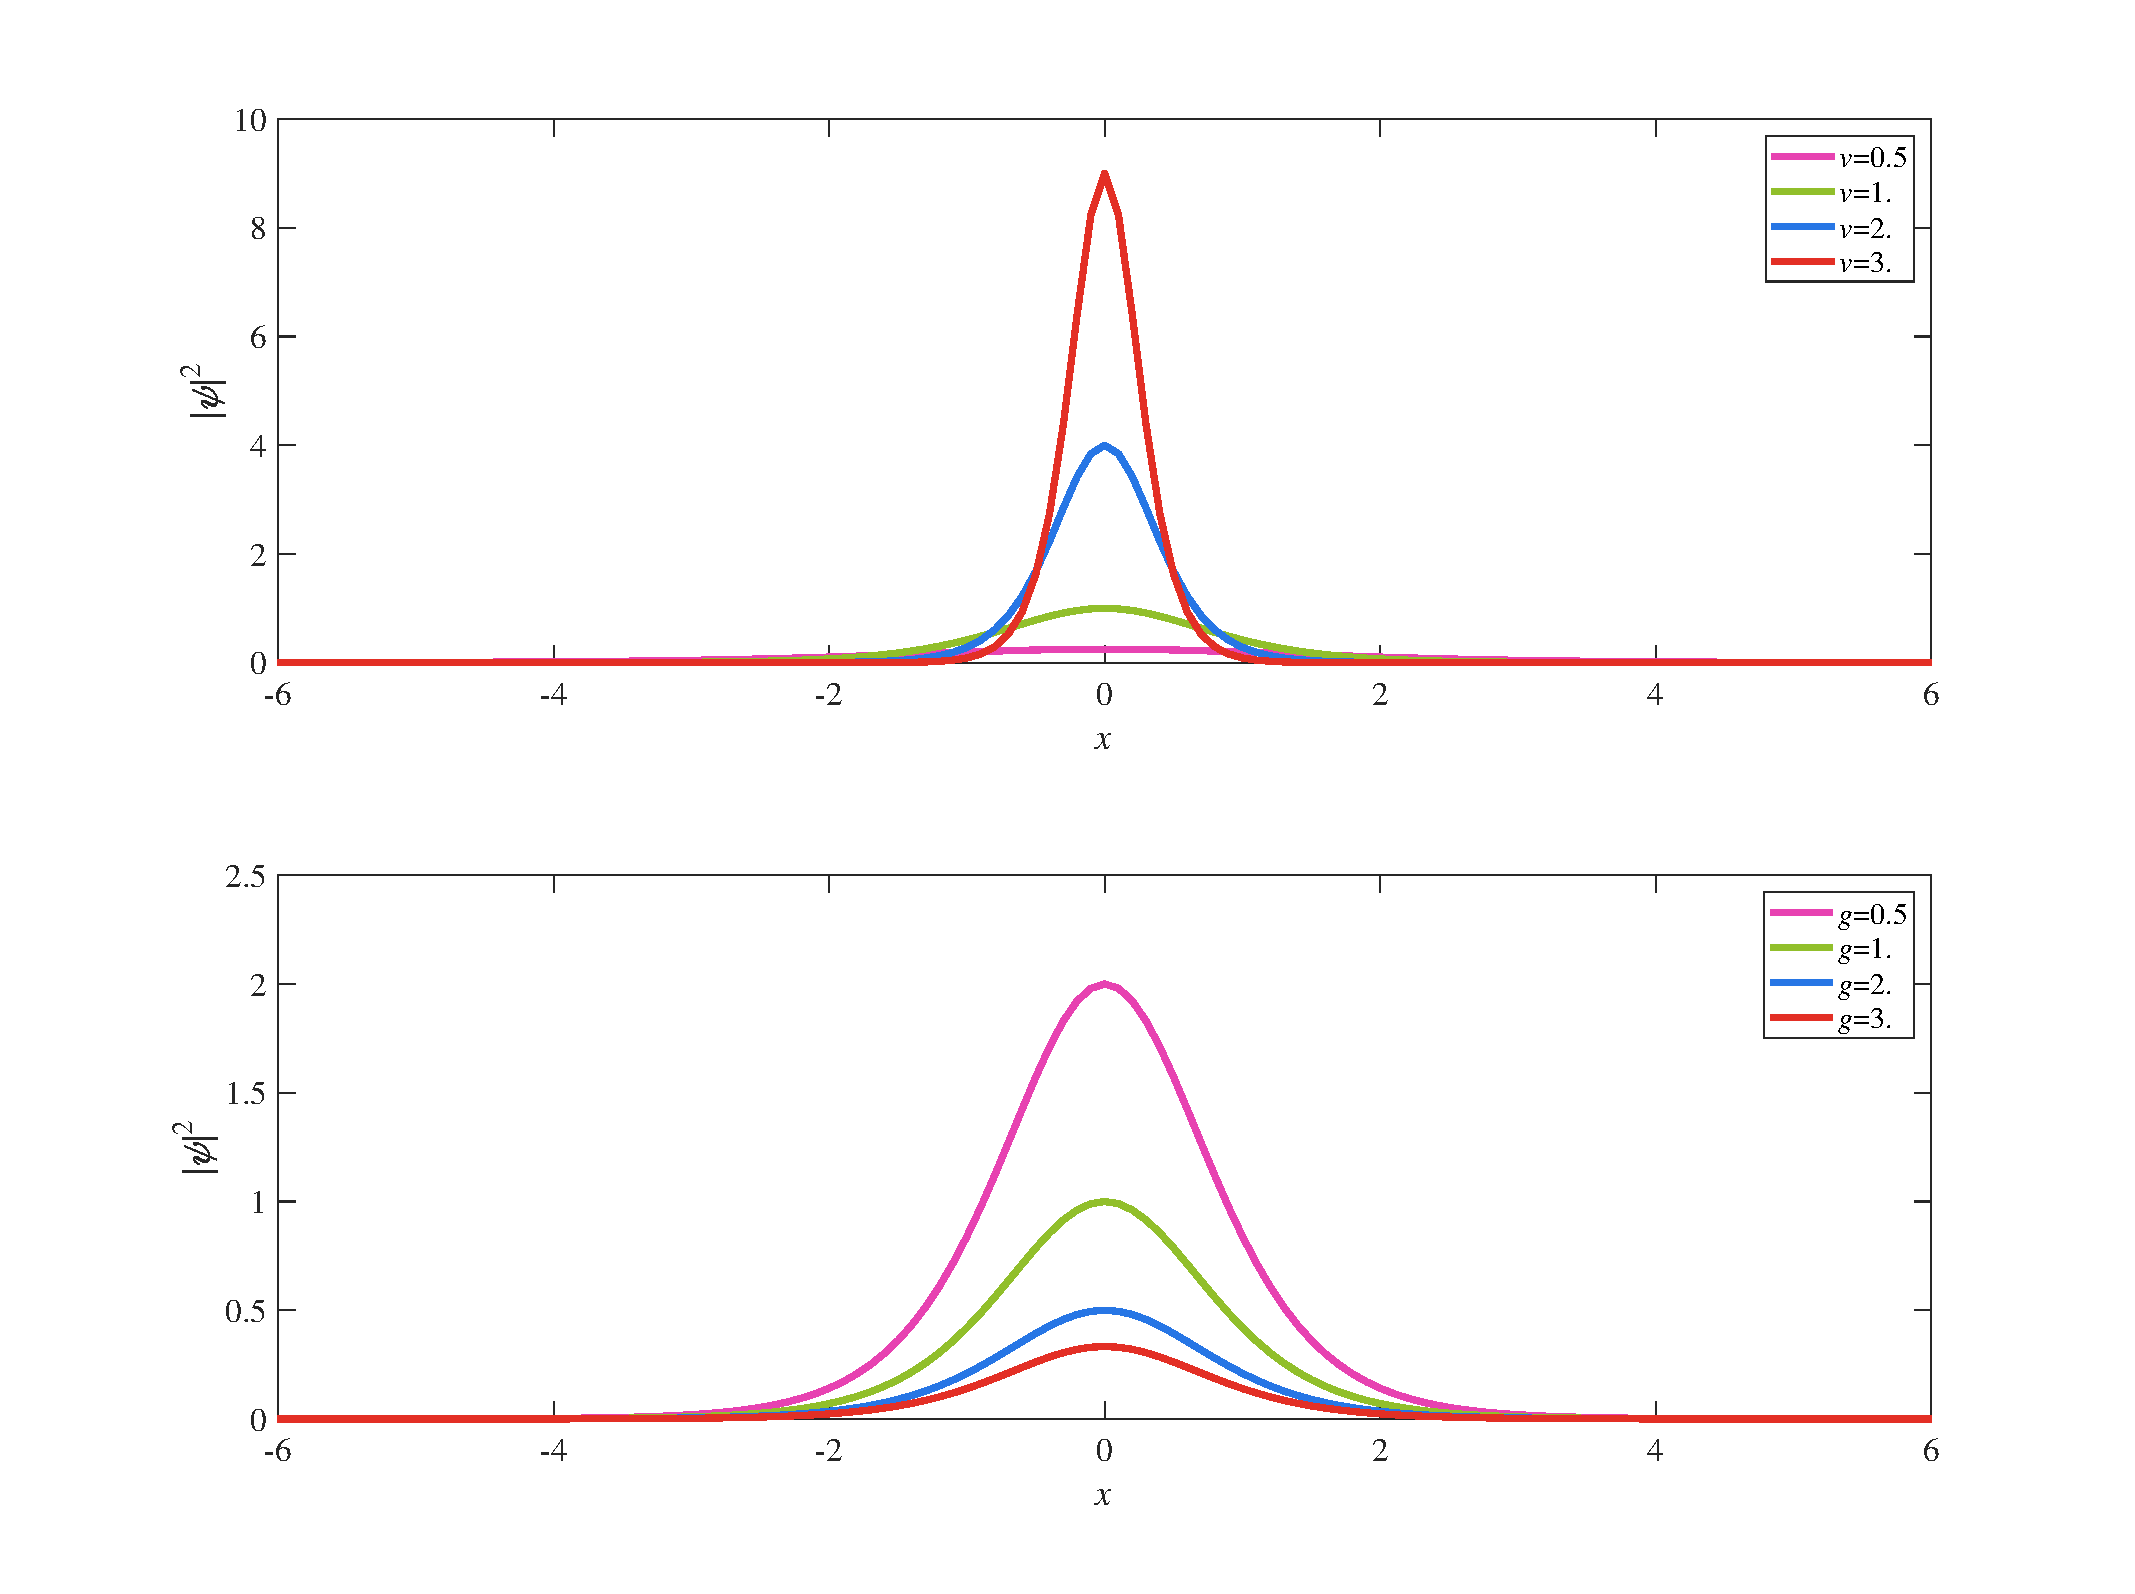
\includegraphics[width=\textwidth]{NLSGSolitonen_1.pdf}
  \caption[L�sungen der nichtlinearen Schr�dinger-Gleichung bei Variation der
  Parameter]{L�sungen der nichtlinearen Schr�dinger-Gleichung f�r verschiedene
    Parameter $v$ und $g$.}
  \label{abb:kontmech_NLSG1}
\end{figure}

Das Soliton steigt um sein Zentrum an und f�llt danach wieder auf den Wert
Null ab.  Die Parameter $v$ und $g$ k�nnen unabh�ngig von einander variiert
werden und haben unterschiedliche Auswirkungen. Gemeinsam ist beiden, dass sie
sehr stark die Amplitude ver�ndern, was f�r die nichtlineare Gleichung zu
erwarten ist. Dabei zeigt sich, dass kleine Werte $v$ zu einem breiten und
flachen Soliton f�hren, gro�e werte zu einem steilen und hohen. Variiert man
den Parameter $g$, der die St�rke der Nichtlinearit�t ausdr�ckt, so findet
man f�r kleine Werte von $g$ ein hohes Soliton, f�r gro�e ein niedriges.

Die Propagation eines Solitons f�r die Parameter $v = 1.5$ und
$g = 0.8$ ist in \figref{kontmech_NLSG2} zu sehen. Die numerische L�sung
(dick gestrichelte Linien) f�hrt auf ein Soliton, das sich in seiner Form und
Gr��e nicht �ndert, sondern ausschlie�lich mit dem Geschwindigkeit $v$ nach
rechts propagiert. Dabei zeigt es f�r jeden Zeitschritt eine sehr gute
�bereinstimmung mit der analytsischen Erwartung \eqref{eq:kontmech_soliton06}.

\begin{figure}
  \centering
  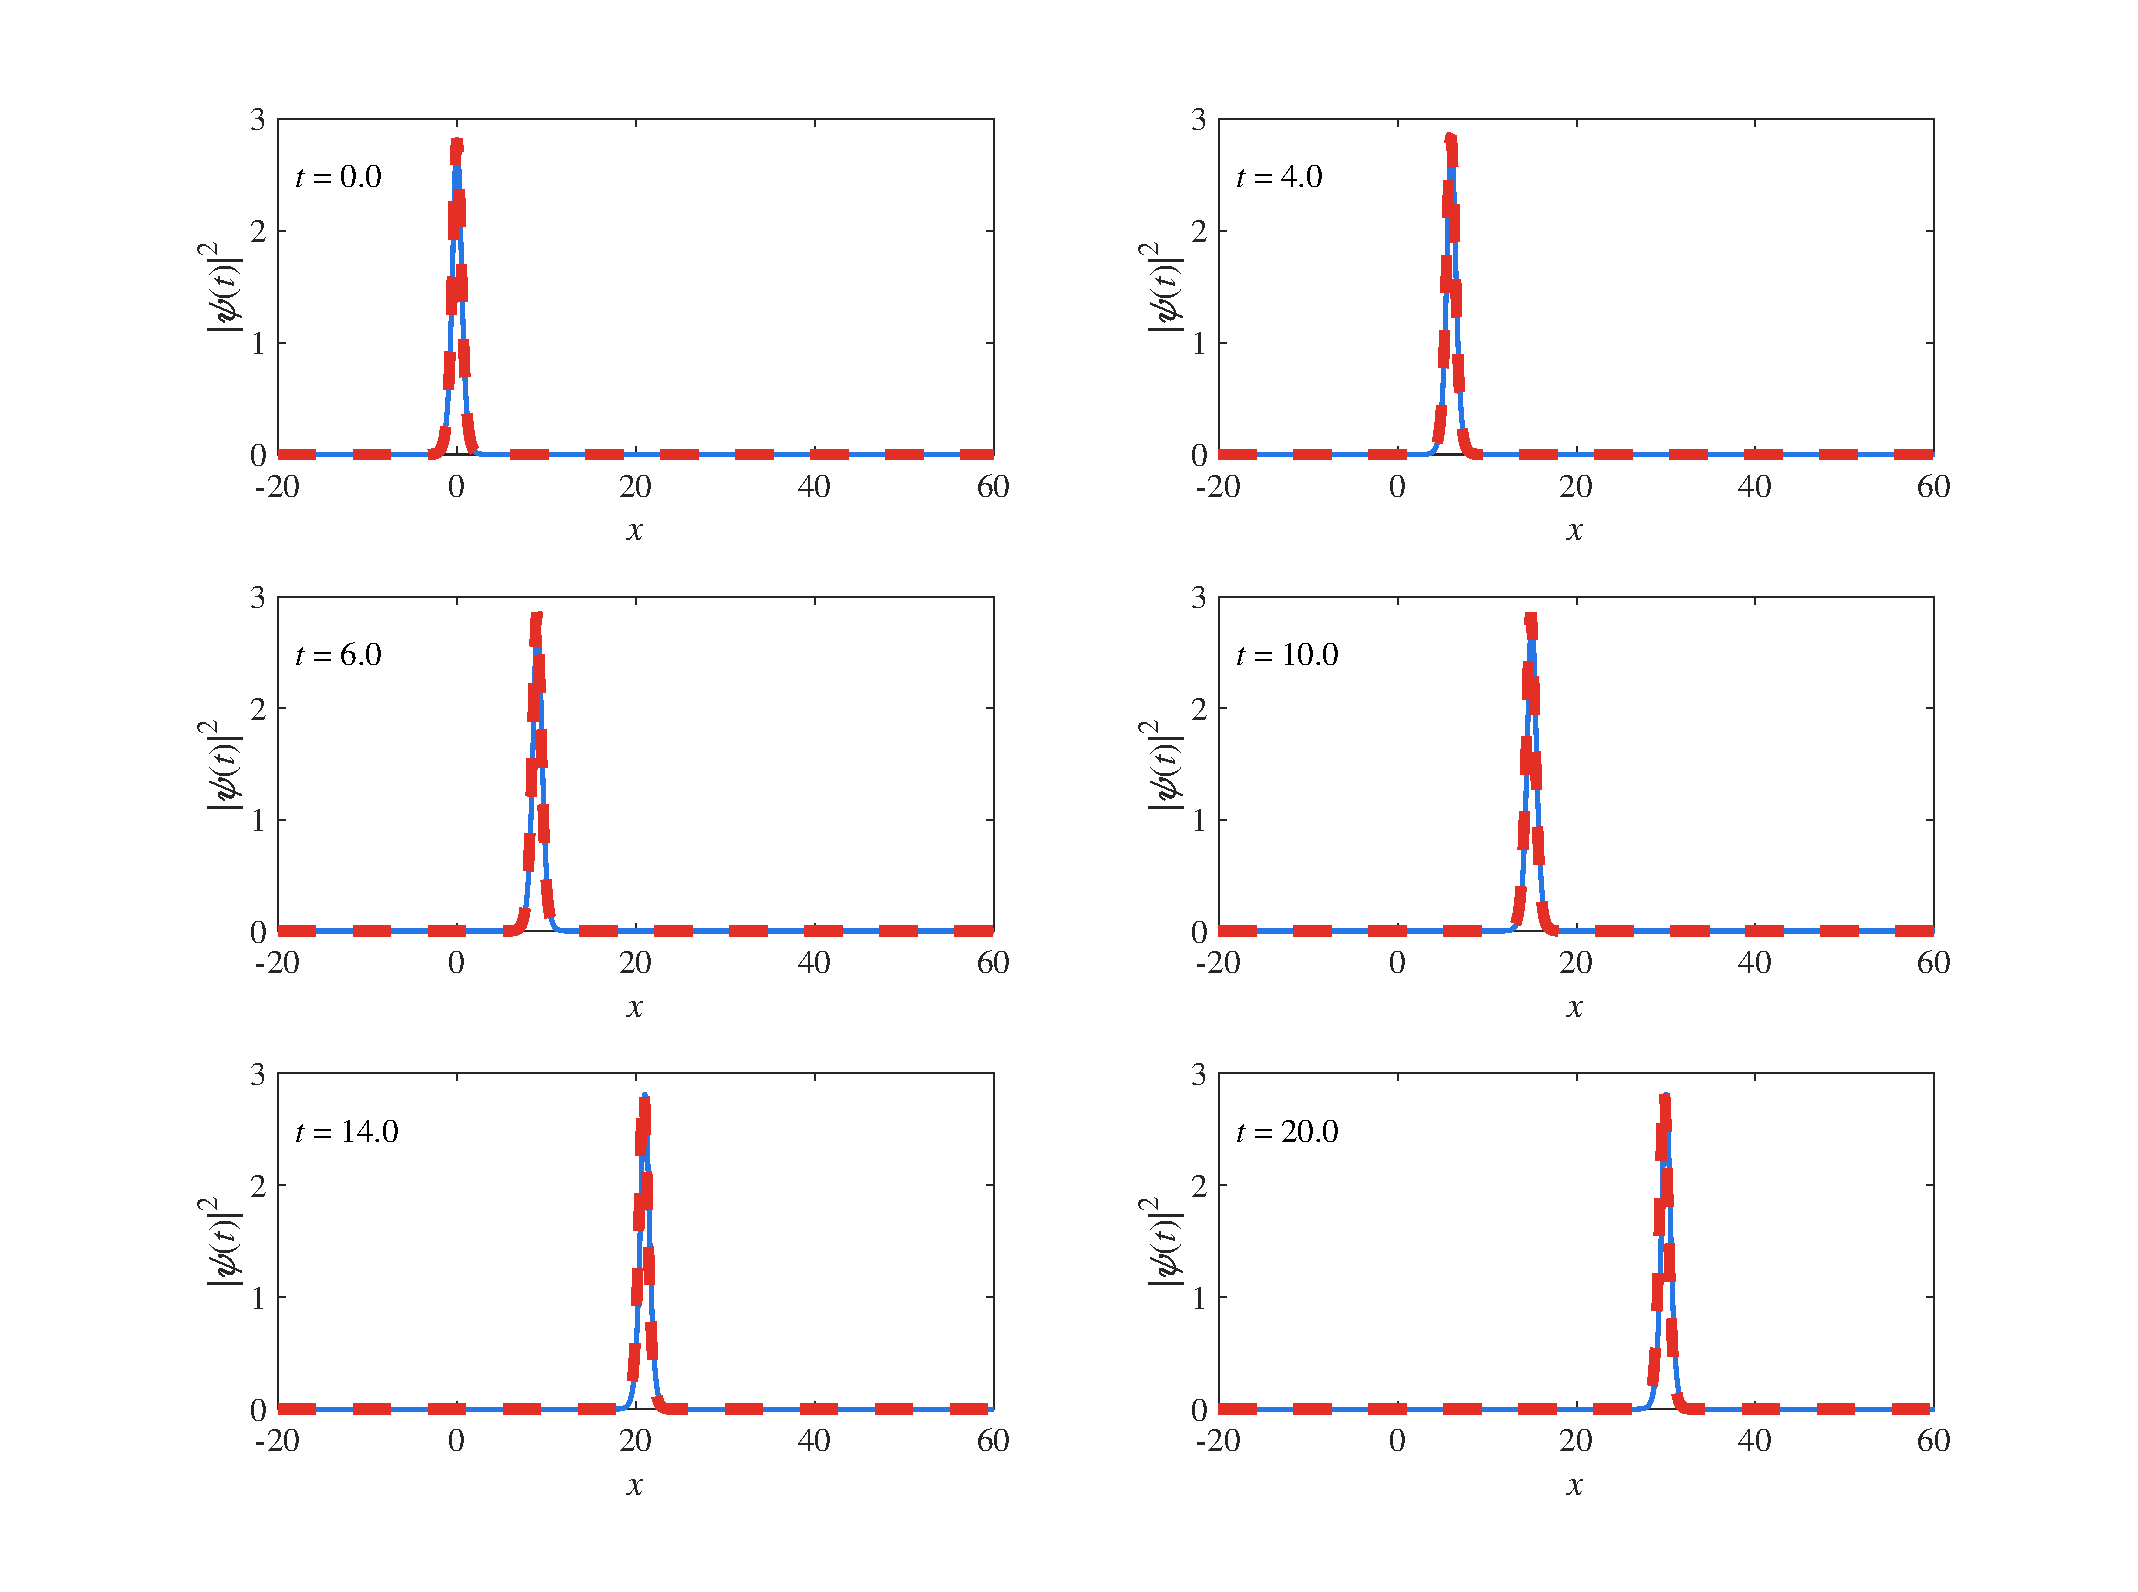
\includegraphics[width=\textwidth]{NLSGSolitonen_2.pdf}
  \caption[Numerische L�sungen der nichtlinearen Schr�dinger-Gleichung]
  {Numerische L�sungen der nichtlinearen Schr�dinger-Gleichung f�r die
    Propagation eines Solitons mit dem Parametern $v = 1.5$ und $g = 0.8$.
    Die Form bleibt erhalten und die numerische Intergration mit der Methode
    der finiten Differenzen (dick gestrichelte Linien) stimmt exakt mit der
    analytischen Form (d�nne durchgezogene Linien) �berein.}
  \label{abb:kontmech_NLSG2}
\end{figure}

Aus dem Vergleich der analytischen und der numersichen L�sung in
\figref{kontmech_NLSG2} k�nnen wir bereits vermuten, dass die analytische
gegebene Funktion \eqref{eq:kontmech_soliton06} eine L�sung der
nichtlinearen Schr�dinger-Gleichung
\begin{equation}
  \im\,\frac{\partial \psi}{\partial t} + \frac{1}{2}\,\frac{\partial^2 \psi}
  {\partial x^2} + g\, \left|\psi\right|^2\,\psi = 0  
  \tag{\ref{eq:kontmech_soliton05}}
\end{equation}
ist. Dies k�nnen und wollen wir nun noch durch eine Rechnung zeigen. Erneut
berechnen wir daf�r zun�chst die ben�tigten Ableitungen,
\begin{subequations}
  \begin{align}
    \frac{\partial \psi(x,t)}{\partial t}
    &= -\frac{A_0}{\tau_0}
      \frac{\sinh\lk \frac{t- x/v}{\tau_0} \rk}{\cosh^2 \lk \frac{t- x/v }
      {\tau_0} \rk} \exp \lek -\im \frac{x}{x_0} \rek \; , \\
    \frac{\partial \psi(x,t)}{\partial x}
    &= \frac{A_0}{v\,\tau_0}
      \frac{\sinh\lk \frac{t- x/v}{\tau_0} \rk}{\cosh^2 \lk \frac{t- x/v }
      {\tau_0} \rk} \exp \lek -\im \frac{x}{x_0} \rek
      - \frac{\im A_0}{x_0} \frac{1}{\cosh \lk \frac{t- x/v}{\tau_0} \rk}
      \exp \lek -\im \frac{x}{x_0} \rek \; , \\
    \frac{\partial^2 \psi(x,t)}{\partial x^2}
    &= -\frac{A_0}{(v\,\tau_0)^2} \frac{1}{\cosh \lk \frac{t- x/v}{\tau_0} \rk}
      \exp \lek -\im \frac{x}{x_0} \rek
      + \frac{2 A_0}{(v\,\tau_0)^2} \frac{\sinh^2\lk \frac{t- x/v}{\tau_0} \rk}
      {\cosh^3 \lk \frac{t- x/v}{\tau_0} \rk} \exp \lek -\im \frac{x}{x_0} \rek
      \notag \\
      &\quad - \frac{2\,\im A_0}{v\,\tau_0\, x_0}
      \frac{\sinh\lk \frac{t- x/v}{\tau_0} \rk}{\cosh^2 \lk \frac{t- x/v }
        {\tau_0} \rk} \exp \lek -\im \frac{x}{x_0} \rek
        - \frac{A_0}{x_0^2} \frac{1}{\cosh \lk \frac{t- x/v}{\tau_0} \rk}
      \exp \lek -\im \frac{x}{x_0} \rek \; .
  \end{align}
\end{subequations}
Eingesetzt in die Differentialgleichung \eqref{eq:kontmech_soliton05}
erh�lt man
\begin{multline}
  -\frac{\im A_0}{\tau_0} \lk 1 + \frac{1}{v\, x_0} \rk
  \frac{\sinh\lk \frac{t- x/v}{\tau_0} \rk}{\cosh^2 \lk \frac{t- x/v }
    {\tau_0} \rk} \exp \lek -\im \frac{x}{x_0} \rek
  + A_0 \Bigg \{ -\frac{1}{2 (v\,\tau_0)^2} \cosh^2 \lk \frac{t- x/v}{\tau_0}
  \rk + \frac{1}{(v\,\tau_0)^2} \sinh^2\lk \frac{t- x/v}{\tau_0} \rk \\
  - \frac{1}{2\, x_0^2} \cosh^2 \lk \frac{t- x/v}{\tau_0} \rk + g |A_0|^2
  \Bigg \}
  \frac{1}{\cosh^3 \lk \frac{t- x/v}{\tau_0} \rk}
  \exp \lek -\im \frac{x}{x_0} \rek = 0 \; .
\end{multline}
Da alle Koeffizienten reell sind und sich die komplexe Exponentialfunktion
k�rzen l�sst, m�ssen relle und imagin�re Vorfaktoren auf der linken Seite
getrennt verschwinden, um die Differentialgleichung erf�llen zu k�nnen. F�r
den imagin�ren Vorfaktor (erster Summand) f�hrt das auf
\begin{subequations}
  \begin{equation}
    x_0 = - \frac{1}{v} \; .
    \label{eq:kontmech_NLSG_par1}
  \end{equation}
  Damit in der geschweiften Klammer keine Funktion mehr vorkommt und die
  Differentialgleichung f�r alle $x$ und $t$ erf�llt sein kann, muss
  \begin{equation}
    \tau_0 = \pm \frac{1}{v^2}
    \label{eq:kontmech_NLSG_par2}
  \end{equation}
  erf�llt sein. Mit diesem $\tau_0$ k�nnen wir
  \begin{multline*}
    -\frac{1}{2 (v\,\tau_0)^2} \cosh^2 \lk \frac{t- x/v}{\tau_0} \rk
    + \frac{1}{(v\,\tau_0)^2} \sinh^2\lk \frac{t- x/v}{\tau_0} \rk
    - \frac{1}{2\, x_0^2} \cosh^2 \lk \frac{t- x/v}{\tau_0} \rk \\
    = -\frac{v^2}{2} \cosh^2 \lk \frac{t- x/v}{\tau_0} \rk
    + v^2 \sinh^2\lk \frac{t- x/v}{\tau_0} \rk
    - \frac{v^2}{2} \cosh^2 \lk \frac{t- x/v}{\tau_0} \rk \\
    = v^2 \Bigg \{ - \cosh^2 \lk \frac{t- x/v}{\tau_0} \rk
    + \sinh^2\lk \frac{t- x/v}{\tau_0} \rk \Bigg \} = -v^2
  \end{multline*}
  zusammenfassen und die gesamte geschweifte Klammer verschwindet f�r
  \begin{equation}
    A_0 = \frac{v}{\sqrt{g}}
    \label{eq:kontmech_NLSG_par3}
  \end{equation}
\end{subequations}
oder jedem komplexen $A_0$ mit demselben Betrag. Damit haben wir aber gezeigt,
dass f�r die gefunden Werte $x_0$, $\tau_0$ und $A_0$ aus den Gleichungen
\eqref{eq:kontmech_NLSG_par1}-\eqref{eq:kontmech_NLSG_par3} die Funktion
\eqref{eq:kontmech_soliton06} eine L�sung der nichtlinearen
Schr�dinger-Gleichung ergibt.

F�r die L�sung mit der Methode der finiten Differenzen  m�ssen wir erneut
die Ableitungen diskretisieren. Ben�tigt werden
\begin{subequations}
  \begin{align}
    \frac{\partial \psi(x_i,t_j)}{\partial t}
    &= \frac{\psi(x_{i},t_{j+1}) - \psi(x_{i},t_{j-1})}{2\Delta t}  \; , \\
    \frac{\partial^2 \psi(x,t)}{\partial x^2}
    &= \frac{\psi(x_{i+1},t_{j}) + \psi(x_{i-1},t_{j}) -2 \psi(x_{i},t_{j})}
      {\Delta x^2}  \; .
  \end{align}
\end{subequations}
Damit l�sst sich die nichtlineare Schr�dinger-Gleichung auf die diskrete Form
\begin{subequations}
  \begin{multline}
    \im \frac{\psi(x_{i},t_{j+1}) - \psi(x_{i},t_{j-1})}{2\Delta t}
    + \frac{1}{2} \frac{\psi(x_{i+1},t_{j}) + \psi(x_{i-1},t_{j})
      -2 \psi(x_{i},t_{j})}{\Delta x^2} \\
    + g |\psi(x_{i},t_{j})|^2 \psi(x_{i},t_{j}) = 0
  \end{multline}
  bringen, was aufgel�st als Interaionsgleichung in der Methode der finiten
  Differenzen geschrieben werden kann als
  \begin{multline}
    \psi(x_{i},t_{j+1}) =  \psi(x_{i},t_{j-1})
    + \im \frac{\Delta t}{\Delta x^2} \left ( \psi(x_{i+1},t_{j})
      + \psi(x_{i-1},t_{j}) -2 \psi(x_{i},t_{j}) \right ) \\
    + 2 \im\,\Delta t \, g |\psi(x_{i},t_{j})|^2 \psi(x_{i},t_{j}) \; .
  \end{multline}
\end{subequations}
Ein Programm, das diese Iteration durchf�hrt, ist in der \matlab{}-Datei
\mlkontmechref{NLSGSolitonen.m} enthalten.

\end{sol} 
\textcolor{blue} {$\rightarrow$ zur} \probref{kontmech_soliton2}.\\
\noindent\rule[1ex]{\textwidth}{0.5pt}  \newpage  \clearpage

%-----------------------------------------------------------------------------------------------------------

\begin{sol}{prob:kontmech_tsunamis}\label{lsg:kontmech_tsunamis} %�bung28
\textbf{Tsunamis}\\ \\

\begin{enumerate}
\item Im Entstehungsgebiet des Erdbebens ist das Wasser etwa $h=\SI{30}
  {\kilo\metre}$ tief. Wir haben es also mit einem Volumen von
  \begin{equation*}
    V = A_\mathrm{Ellipse}\cdot h = \pi\cdot \SI{100}{\kilo\metre} \cdot
    \SI{1000}{\kilo\metre} \cdot \SI{30}{\kilo\metre}
    = \SI{3e6}{\kilo\metre^3} = \SI{3e15}{\metre^3}
  \end{equation*}
  oder einer Masse von
  \begin{equation*}
    m = \varrho \cdot V = \SI{1020}{\kilo\gram\per\metre^3} \cdot
    \SI{3e15}{\metre^3} = \SI{3.06e18}{\kilo\gram}
  \end{equation*}
  zu tun. In einer ersten, sehr naiven Modellierung der tektonischen
  Plattenbewegung kann man �berlegen, um welche H�he man diese Wassermenge
  anheben muss, um in ihr die vermutete Energie von
  \begin{equation*}
    E = 475\cdot \SI{4.183e15}{\joule} = \SI{1.987e18}{\joule}
  \end{equation*}
  aufzubringen. Auf diesem Weg erh�lt man eine H�he von
  \begin{equation*}
    h = \frac{E}{m \cdot g} = \frac{\SI{1.987e18}{\joule}}{\SI{3.06e18}
      {\kilo\gram}\cdot\SI{9.81}{\metre\per\second^2}} \approx \SI{6.6}
    {\centi \metre} \; .
  \end{equation*}
  Nat�rlich geschieht dies nicht langsam und es wird nicht die gesamte
  Wassermenge angehoben. Durch den enormen Wasserdruck in der Tiefe sind vor
  allem seitliche Ausweichbewegungen zu erwarten, die die Bewegung der St�rung
  vom Zentrum weg in Gang bringen. Die kinetische Energie, die in das Wasser
  geht, sorgt jedoch daf�r, dass die oberen Schichten sich deutlich st�rker
  heben, und wurden f�r das hier behandelte Beben auf $\SI{10}{\metre}$
  gesch�tzt.

\item In Referenz \cite{Constantin2007} aus der Aufgabenstellung werden
  Gr�nde genannt, die gegen Solitonen sprechen. Insbesondere wird darauf
  eingegangen, dass Tsunamis selten der H�he nach geordnet auf eine
  K�ste treffen. Lie�e sich die gesamte Ausbreitung eines Tsunamis durch
  die Korteweg-de-Vries-Gleichung beschreiben, m�sste sich ein Tsunami
  in Solitonen zerlegen. Die h�chsten Wellenberge m�ssten dabei
  die h�chste Ausbreitungsgeschwindigkeit besitzen und am schnellsten
  auf die K�ste treffen, wie dies z.B. aus 
  \figref{kontmech_KdVSolitonVergleichc}, \figref{kontmech_KdVSolitonSumme1}
  und \figref{kontmech_KdVSolitonInteraktion} in L�sung
  \ref{lsg:kontmech_soliton1} geschlossen werden kann. Auch werden reine
  Wassersenken beobachtet, die sich nicht in der Korteweg-de-Vries-Gleichung
  finden.

  Tats�chlich kann man bei gro�en Wassertiefen wie den Entstehungsgebieten
  der Tsunamis davon ausgehen, dass die Nichtlinearit�t der
  Kroteweg-de-Vries-Gleichung aufgrund der geringen Amplitude nur von
  geringer Bedeutung ist und nicht unbedingt Solitonen vorliegen m�ssen. Eine
  lineare Wellentheorie k�nnte die Ausbreitung hier erkl�ren -- insbesondere,
  da nach der Erkl�rung in Referenz \cite{Constantin2007} typische
  Tusinamis nicht von einer Disperson betroffen sind. Also w�rde auch eine
  lineare Wellengeleichung den solit�ren St�rungen im Wasser nicht
  widersprechen. Sp�testens wenn der Tsunami auf die K�ste trifft, m�ssten
  aber die nichtliearen Effekte der Korteweg-de-Vries-Gleichung greifen und
  sie m�sste eine vern�nftige Beschreibung darstellen.

\item Unabh�ngig von der vorherigen Diskussion m�chten wir betrachten, wie
  die Korteweg-de-Vries-Gleichung einen Tsunami als ein auf die K�ste
  treffendes Soliton beschreiben kann. Daf�r m�ssen wir die KdV-Gleichung
  zun�chst aber in ihren urspr�nglichen physikalischen Kontext als Gleichung
  f�r Wellen im flachen Wasser �berf�hren, denn wir ben�tigen den Zusammenhang
  zur Wassertiefe, die sich an der K�ste �ndert.

  Die Formulierung von Korteweg und de Vries \cite{Korteweg1895} wird
  geschrieben als 
  \begin{equation}
    \frac{\partial \psi}{\partial t} = \frac{3}{2} \sqrt{\frac{g}{d}}
    \lk \psi \frac{\partial \psi}{\partial x} + \frac{2}{3} \alpha
    \frac{\partial \psi}{\partial x} + \frac{1}{3} \sigma \frac{\partial^3
      \psi}{\partial x^3} \rk
    \label{eq:kontmech_KdVOriginal}
  \end{equation}
  mit der Schwerebeschleunigung $g$, der Wassertiefe $d$ und dem
  Parameter
  \begin{equation}
    \sigma = \frac{d^3}{3} - \frac{T\,d}{\varrho\,g} \; ,
  \end{equation}
  in dem zus�tzlich die Oberfl�chenspannung $T$ und die Dichte $\varrho$
  des Wassers vorkommen. Der weitere Parameter $\alpha$ ist beliebig und
  wird nur ben�tigt, um die exakte Geschwindigkeit des Solitons einzustellen.
  Da dieser Zusammenhang f�r unsere Fragestelltung nach der Form des Solitons
  an der K�ste nicht relevant ist, setzen wir im weiteren Verlauf $\alpha = 0$.

  Ein Soliton, das Gleichung \eqref{eq:kontmech_KdVOriginal} l�st, hat die
  Form 
  \begin{equation}
    \psi(x,t) = 2 c \sqrt{\frac{d}{g}} \;
    \sech^2\lek \frac{1}{2}\; \sqrt{\frac{2c}{\sigma}\sqrt{\frac{d}{g}}}
    \lk x-ct \rk \rek \,.
    \label{eq:kontmech_KdVOriginalSoliton}
  \end{equation}
  Hier erkennt man deutlich, dass das Soliton von der Wassertiefe abh�ngt.
  Insbesondere werden die H�he, aber auch die Breite von $d$ beeinflusst.
  
  Die numerische L�sung der partiellen Differentialgleichung f�r eine
  ver�nderliche Wassertiefe $d$ wird in der \matlab{}-Datei
  \mlkontmechref{KdVTsunami.m} bewerkstelligt. Eine L�sung ist in
  \figref{kontmech_KdVTsumami} dargestellt.
  
  \begin{figure}
    \centering
    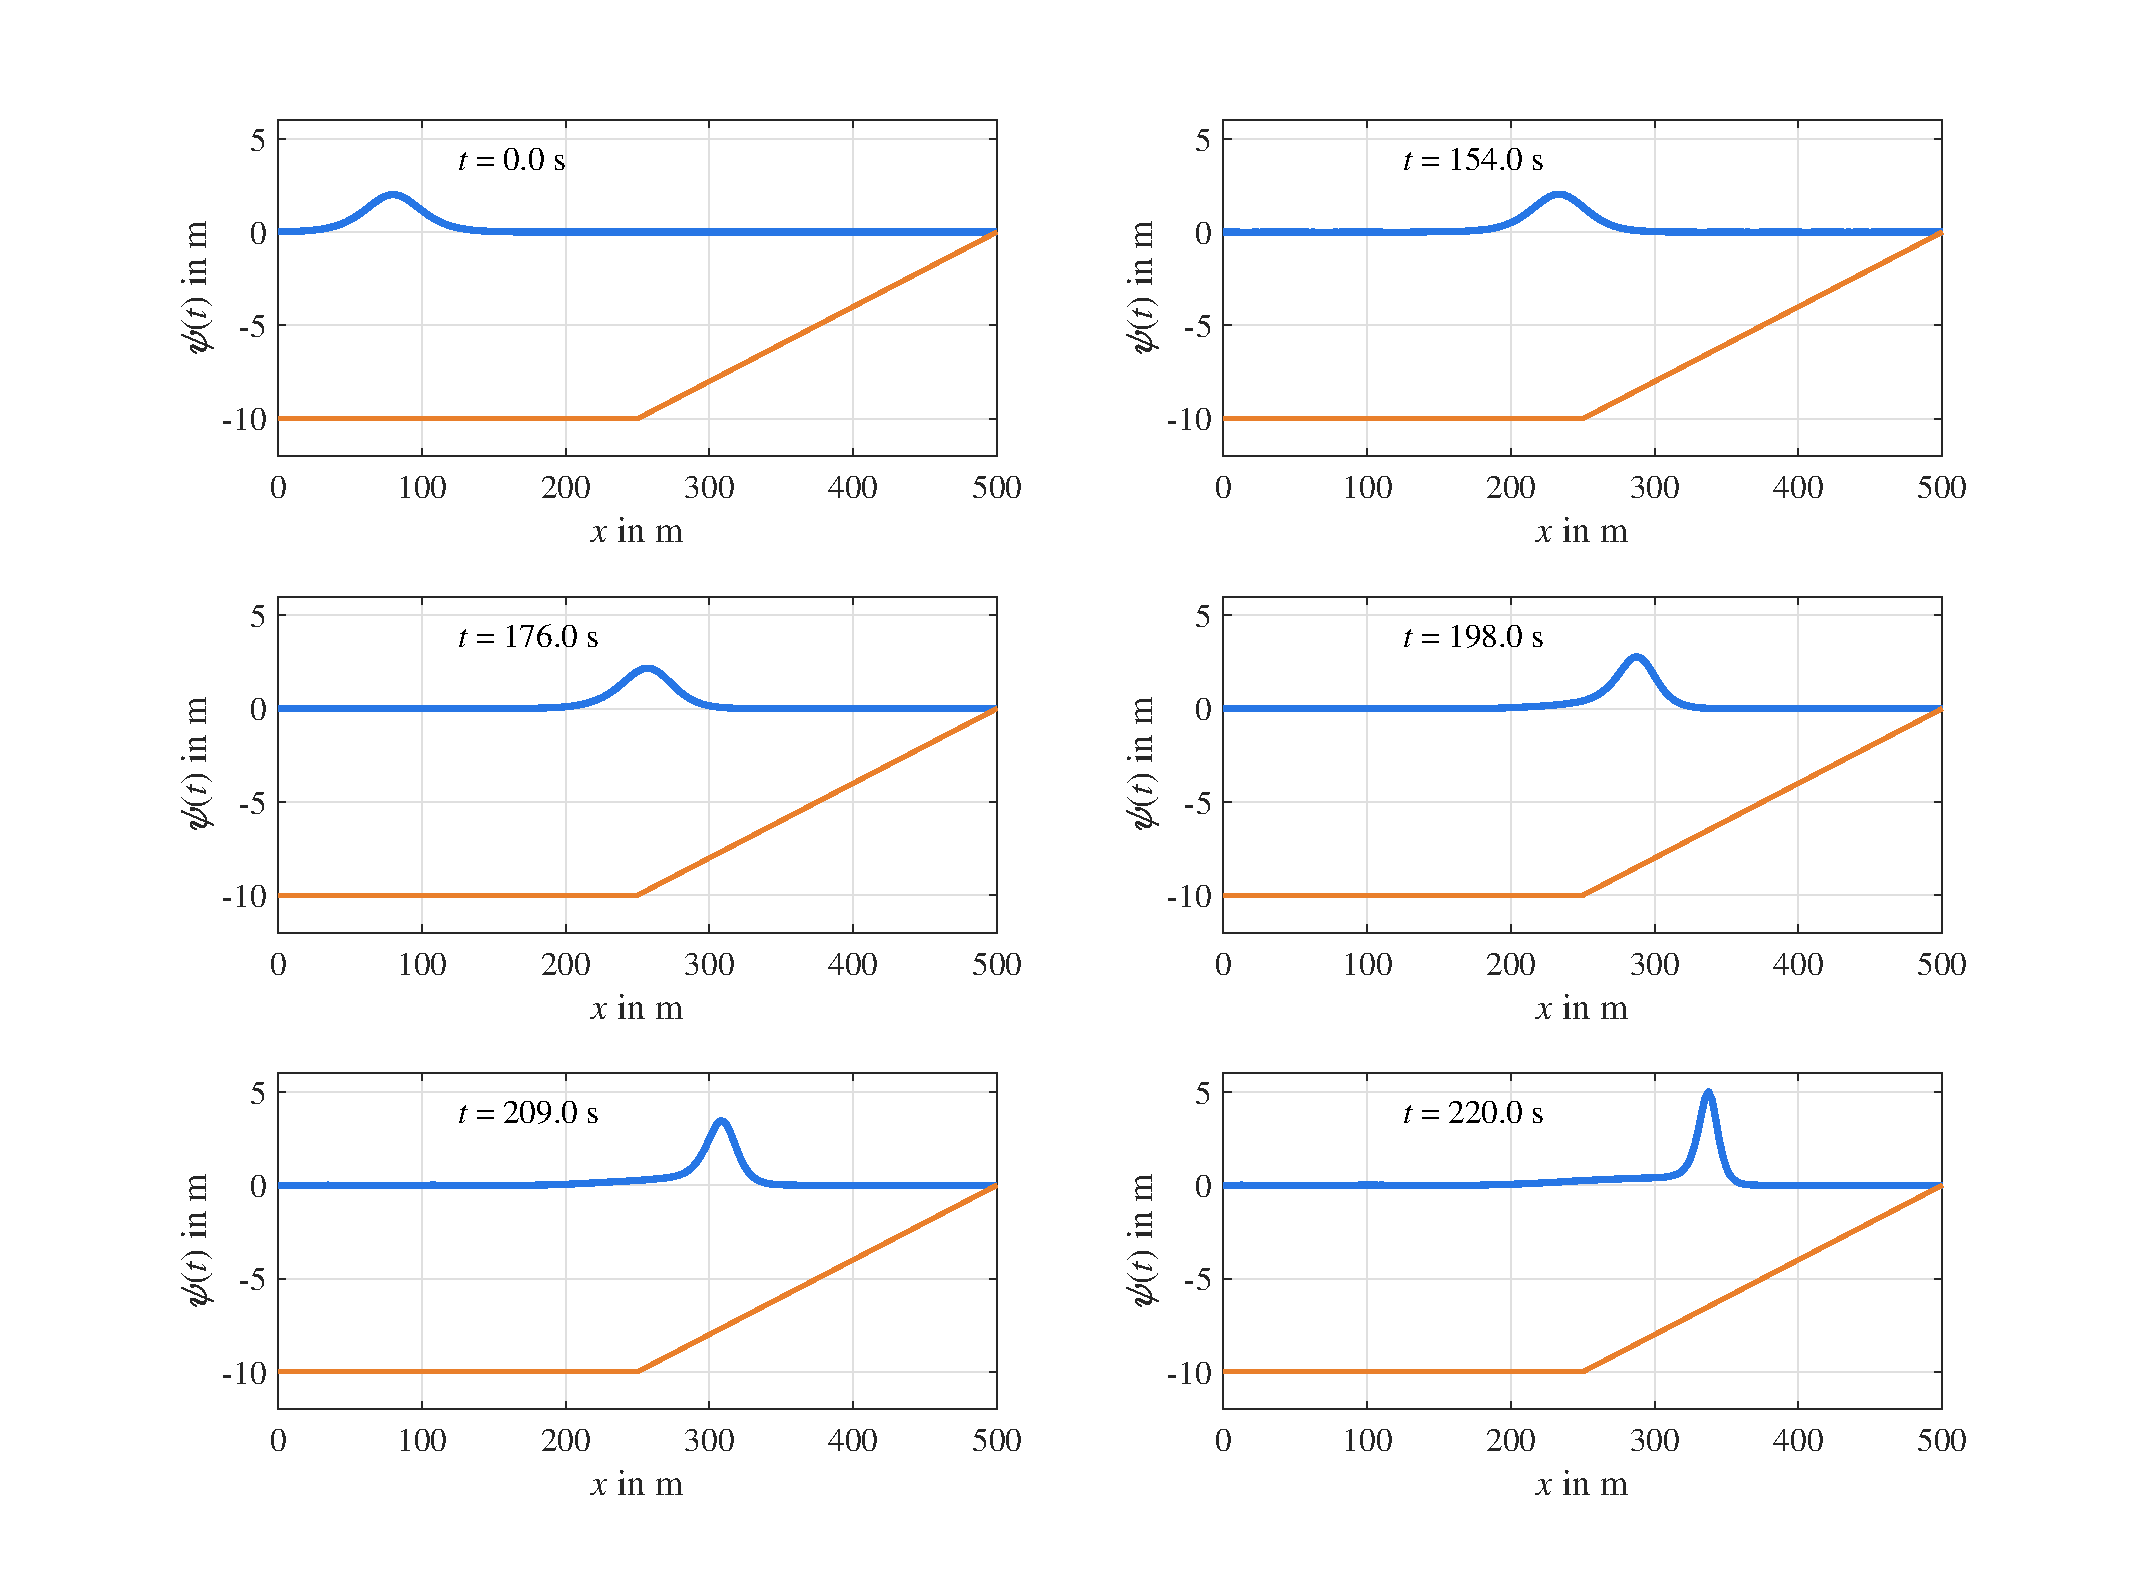
\includegraphics[width=\textwidth]{KdVTsunami.pdf}
    \caption[Eine Soliton-L�sung der Korteweg-de-Vries-Gleichung l�uft
    auf eine K�ste zu.]
    {Eine Soliton-L�sung der Korteweg-de-Vries-Gleichung aus einem Bereich mit
      einem Flachen Meeresgrund l�uft auf eine K�ste zu. Es entsteht nach und
      nach eine immer h�here St�rung der Wasseroberfl�che, die sich in Richtung
      der K�ste zu einer steilen Wand aufstellt.}
    \label{abb:kontmech_KdVTsumami}
  \end{figure}

  Die beispielhafte Rechnung geht von Salzwasser mit der Dichte von
  $\varrho = \SI{1020}{\kilo\gram\per\metre^3}$ und einer Oberfl�chenspannung
  von $T = \SI{0.07495}{\newton\per\metre}$ aus. Zun�chst hat das Wasser
  eine Tiefe von $d = \SI{10}{\metre}$, die schlie�lich auf Null abf�llt.
  Man erkennt, wie sich die Form des Solitons in K�stenn�he ver�ndert. Es
  wird h�her und verliert an Breite. Von der K�ste aus gesehen steigt es
  steil an. Hinter dem Maximum f�llt es wieder steil ab, jedoch gibt es einen
  flach auslaufenden Bereich. Blickt man von der K�ste aus auf ein solches
  Soliton, hat man den Eindruck, dass es sich zu einer Wand aufstellt.
\end{enumerate}

\end{sol} 
\textcolor{blue} {$\rightarrow$ zur} \probref{kontmech_tsunamis}.\\
\noindent\rule[1ex]{\textwidth}{0.5pt}  \newpage  \clearpage

% ----------------------------------------------------------------------------------------------------------
% ----------------------------------------------------------------------------------------------------------

 
%
%\chapter{Anhang} \label{chap:solman_appendix}
%\addcontentsline{toc}{part}{Anhang}
%\setcounter{chapter}{0}

%%\documentclass[makeidx,envcountchap,graybox,deutsch,ngerman,sectrefs]{svmono}
%\documentclass[envcountchap,graybox,deutsch,sectrefs]{svmono}
%%%%% eigene tempor�re Abk�rzungsliste, f�r die Zeit, bis einheitliche Schreibungen bestehen
\usepackage{tempshort}
%%  Von Springer empfohlene Pakete %% 
%%\documentclass[envcountsect,graybox,deutsch,sectrefs]{svmono}
\usepackage{chapterbib}
\usepackage{type1cm}
\usepackage[ansinew]{inputenc}
\usepackage{babel}
\usepackage[pdftex]{graphicx} %PDF-Vektorgrafiken einbinden
\usepackage{newtxtext} %Typischer Springer-Font
\usepackage{newtxmath}
\usepackage{multicol}
\usepackage[bottom]{footmisc} %Platziert alle Fu�noten unten  
\usepackage[nobreak]{cite}
%\usepackage{biblatex}
\usepackage{cancel}
\usepackage[absolute]{textpos}
\usepackage{graphicx}
\usepackage{pdfpages}

%\usepackage{floatrow}
%\usepackage{mwe}
\usepackage[figuresright]{rotating}
\usepackage{bigints}
\let\laplace\relax  % Vermeidung der Fehlermeldung "\laplace already defined."
\usepackage{trfsigns}
\usepackage{amsmath}
\usepackage{tabulary}
\usepackage{tabularx}

%%  Eigene Pakete %%
\usepackage{adjustbox}
\usepackage{wasysym}
\usepackage{gensymb}
\usepackage{float}
\usepackage{caption}
\usepackage[left=5cm,right=4cm,top=3cm,bottom=4cm,includeheadfoot]{geometry}

%\usepackage{wasysym}
%\usepackage{bigints}
%\usepackage{esint}
%\usepackage{relsize,exscale}

\usepackage{mathtools}   % Vermeidung der Fehlermeldung "Undefined control sequence \coloneqq."


% header and footer
\usepackage{fancyhdr}
\pagestyle{fancy}
\fancyhead[LE,RO]\thepage
\renewcommand{\sectionmark}[1]{\markright{\thesection.\ #1}}
%\fancyhead[LO]{\nouppercase\leftmark}
%\fancyhead[RE]{\nouppercase\rightmark}
\fancyhead[LO]{\nouppercase\rightmark}
\fancyhead[RE]{\nouppercase\leftmark}
\fancyfoot{}
% svmono hat offenbar irgendwas merkw�rdig definiert, darum mu� hier verbreitert werden
%\addtolength\headwidth{25pt}
\setlength{\headheight}{25pt}

%% Units
\usepackage{siunitx}
\sisetup{
  locale = US,
  per-mode = reciprocal, %symbol, % | reciprocal | fraction | ?
  exponent-product = \cdot,
  separate-uncertainty,
  %exponent-to-prefix,
  %prefixes-as-symbols = false,
  %list-units = brackets,% | single | repeat
  %range-units = brackets,% | single | repeat
  %multi-part-units = brackets,% | single | repeat
}
\usepackage{chngcntr}
\usepackage{booktabs}
\usepackage{slashed}
\usepackage{listings}
\usepackage{color} %red, green, blue, yellow, cyan, magenta, black, white
%\usepackage{color} %Einfache Farbendefinition -> von Graybox-Option ben�tigt
\usepackage{multirow}
\usepackage{longtable} %Tabellen �ber mehrere Seiten hinweg
\usepackage{framed} % von Graybox-Option ben�tigt
\usepackage[shortlabels]{enumitem} %Erweiterte Aufz�hloptionen
\usepackage{array}
\usepackage[xindy]{imakeidx} %Wortindex und Personenindex erstellen

\usepackage[hyphens]{url}
%\usepackage[breaklinks,colorlinks=true,linkcolor=black,urlcolor=blue,citecolor=black,filecolor=green,hyperfootnotes=false]{hyperref}
\usepackage[                                    %Hyperref erstellt ein Bookmark/Lesezeichen im PDF. siehe https://www.namsu.de/Extra/pakete/Hyperref.html
bookmarksopen=true,															%Das Lesezeichen ist ge�ffnet beim �ffnen der PDF.
bookmarksnumbered=true,                         %Zahlen werden im Bookmark angezeigt.   
plainpages=false,
pdfpagelabels,
colorlinks=true,                                %Links werden farbig dargestellt.
linkcolor=black, citecolor=black, urlcolor=cyan %Farben definieren.
]{hyperref}                                     %Sollte als letztes eingebunden werden, da es sehr viele Verweise und �nderungen erzeugt. Das Packet ist sehr stark, aber auch umfangreich ist. 

%\usepackage[breaklinks,colorlinks=true,linkcolor=black,urlcolor=blue,citecolor=black,filecolor=green,hyperfootnotes=false]{hyperref}
%\usepackage[breaklinks,colorlinks=true,linkcolor=black,urlcolor=blue,citecolor=black,filecolor=green,hyperfootnotes=false
            %pdftex,
            %pdfauthor={Kaschke, Cartarius},
            %pdftitle={Finger�bungen der Physik}
            %pdfsubject={Ein Repetitorium und �bungsbuch zu im Studium wenig behandelten Kapiteln der Physik mit ausf�hrlich behandelten Problemen und MATLAB-Programmen},
            %pdfkeywords={Physik, Mechanik}
            %]{hyperref}
\pdfminorversion=5

\usepackage{hypcap}
\usepackage[record,section=section,stylemods={mcols},automake]{glossaries-extra}
\usepackage{glossary-longextra}
%\usepackage{glossary-bookindex}
%\makeindex
\setglossarystyle{long-name-sym-desc-loc}
\setabbreviationstyle[acronym]{long-short}

\definecolor{killA}{rgb}{.7,.3,.3}
\newcommand\killA[1]{\bgroup\color{killA}{\cancel{#1}}\egroup}
\newcommand\killB[1]{\bgroup\color{cyan!30!black}{\cancel{#1}}\egroup}

% typographisch korrekte Abk�rzungen (needs to be loaded after hyperref)
\usepackage{abbrev}
\newglossary*{bew}{Glossar}
\newglossary*{hm}{Glossar}
\newglossary*{adyn}{Glossar}
\newglossary*{kontmech}{Glossar}
\newglossary*{aero}{Glossar}
\newglossary*{edyn}{Glossar}
\newglossary*{spo}{Glossar}
\newglossary*{optbas}{Glossar}
\newglossary*{optger}{Glossar}
\newglossary*{optatm}{Glossar}
\newglossary*{optspez}{Glossar}
\GlsXtrLoadResources[src={bew/gloss},type=bew]
\GlsXtrLoadResources[src={hm/gloss},type=hm]
\GlsXtrLoadResources[src={adyn/gloss},type=adyn]
\GlsXtrLoadResources[src={kontmech/gloss},type=kontmech]
\GlsXtrLoadResources[src={aero/gloss},type=aero]
\GlsXtrLoadResources[src={spo/gloss},type=spo]
\GlsXtrLoadResources[src={edyn/gloss},type=edyn]
\GlsXtrLoadResources[src={optbas/gloss},type=optbas]
\GlsXtrLoadResources[src={optger/gloss},type=optger]
\GlsXtrLoadResources[src={optatm/gloss},type=optatm]
\GlsXtrLoadResources[src={optspez/gloss},type=optspez]
\glssetcategoryattribute{bew}{indexname}{true}
%\renewcommand\index\newterm
%\newcolumntype{g}[1]{>{\RaggedRight\hspace{0pt}}p{#1}}
%\renewcommand\glslongextraNameAlign{g}
\renewcommand\glslongextraLocationAlign{@{\ ~\ }>{\raggedright}p{\glspagelistwidth}}
\definecolor{gls}{rgb}{.4,.4,.5}
\renewcommand*{\glstextformat}[1]{\textcolor{gls}{#1}}

%Absatzregeln
\clubpenalty = 30000 %Keine einzelnen Absatzzeilen
\widowpenalty = 30000
\setlength{\parindent}{0em} 
\newcolumntype{L}[1]{>{\raggedright\arraybackslash}p{#1}}
\newcolumntype{C}[1]{>{\centering\arraybackslash}p{#1}}
\newcolumntype{R}[1]{>{\raggedleft\arraybackslash}p{#1}}

\usepackage{xstring}

\newcommand\mfile[2]{%
\saveexpandmode\noexpandarg
\StrSubstitute{#2}{_}{\_}[\tmpname]
\restoreexpandmode
\href{MatlabDateien/\chapname/#1\tmpname}{\tmpname}}

%%% Hyperlinks zu MATLAB Dateien
%\newcommand\mlref[1]{\mfile{}{#1}}
%\newcommand\mlinclref[1]{\mfile{IncludeFolder/}{#1}}
%\newcommand\mldataref[1]{\mfile{Data/}{#1}}

%%% .. f�r ein Verzeichnis hoch
%%% . f�r aktuelle Verzeichnis
%% lokal: MatlabDateien/bew
%\newcommand\mlbewref[1]{\href{MatlabDateien/bew/#1}{#1}}
%% git: https://github.com/sn-code-inside/fingeruebungen-physik/tree/main/bew

\newcommand{\mlrefwithindex}[2]{%
  \index[mfiles]{#2}%   <-- Eintrag im M-File-Index mit aktueller Seitenzahl
  \href{https://github.com/sn-code-inside/fingeruebungen-physik/tree/main/#1/#2}{#2}%
}


%\newcommand\mlbewref[1]{\href{https://github.com/sn-code-inside/fingeruebungen-physik/tree/main/bew/#1}{#1}}
%\newcommand\mlbewdref[1]{\href{https://github.com/sn-code-inside/fingeruebungen-physik/tree/main/bew/Data/#1}{#1}}
%\newcommand\mlbewiref[1]{\href{https://github.com/sn-code-inside/fingeruebungen-physik/tree/main/bew/IncludeFolder/#1}{#1}}
%\newcommand\mlkontmechref[1]{\href{https://github.com/sn-code-inside/fingeruebungen-physik/tree/main/kontmech/#1}{#1}}
%\newcommand\mlkontmechdref[1]{\href{https://github.com/sn-code-inside/fingeruebungen-physik/tree/main/kontmech/Data/#1}{#1}}
%\newcommand\mlkontmechiref[1]{\href{https://github.com/sn-code-inside/fingeruebungen-physik/tree/main/kontmech/IncludeFolder/#1}{#1}}
%\newcommand\mlhmref[1]{\href{https://github.com/sn-code-inside/fingeruebungen-physik/tree/main/hm/#1}{#1}}
%\newcommand\mlhmdref[1]{\href{https://github.com/sn-code-inside/fingeruebungen-physik/tree/main/hm/Data/#1}{#1}}
%\newcommand\mlhmiref[1]{\href{https://github.com/sn-code-inside/fingeruebungen-physik/tree/main/hm/IncludeFolder/#1}{#1}}
%\newcommand\mladynref[1]{\href{https://github.com/sn-code-inside/fingeruebungen-physik/tree/main/adyn/#1}{#1}}
%\newcommand\mladyndref[1]{\href{https://github.com/sn-code-inside/fingeruebungen-physik/tree/main/adyn/Data/#1}{#1}}
%\newcommand\mladyniref[1]{\href{https://github.com/sn-code-inside/fingeruebungen-physik/tree/main/adyn/IncludeFolder/#1}{#1}}
%\newcommand\mledynref[1]{\href{https://github.com/sn-code-inside/fingeruebungen-physik/tree/main/edyn/#1}{#1}}
%\newcommand\mledyndref[1]{\href{https://github.com/sn-code-inside/fingeruebungen-physik/tree/main/edyn/Data/#1}{#1}}
%\newcommand\mledyniref[1]{\href{https://github.com/sn-code-inside/fingeruebungen-physik/tree/main/edyn/IncludeFolder/#1}{#1}}
%\newcommand\mloptbasref[1]{\href{https://github.com/sn-code-inside/fingeruebungen-physik/tree/main/optbas/#1}{#1}}
%\newcommand\mloptbasdref[1]{\href{https://github.com/sn-code-inside/fingeruebungen-physik/tree/main/optbas/Data/#1}{#1}}
%\newcommand\mloptbasiref[1]{\href{https://github.com/sn-code-inside/fingeruebungen-physik/tree/main/optbas/IncludeFolder/#1}{#1}}
%\newcommand\mloptspezref[1]{\href{https://github.com/sn-code-inside/fingeruebungen-physik/tree/main/optspez/#1}{#1}}
%\newcommand\mloptspezdref[1]{\href{https://github.com/sn-code-inside/fingeruebungen-physik/tree/main/optspez/Data/#1}{#1}}
%\newcommand\mloptspeziref[1]{\href{https://github.com/sn-code-inside/fingeruebungen-physik/tree/main/optspez/IncludeFolder/#1}{#1}}

\newcommand\mlbewref[1]{\mlrefwithindex{bew}{#1}}
\newcommand\mlbewdref[1]{\mlrefwithindex{bew/Data}{#1}}
\newcommand\mlbewiref[1]{\mlrefwithindex{bew/Include}{#1}}
\newcommand\mlkontmechref[1]{\mlrefwithindex{kontmech}{#1}}
\newcommand\mlkontmechdref[1]{\mlrefwithindex{kontmech/Data}{#1}}
\newcommand\mlkontmechiref[1]{\mlrefwithindex{kontmech/Include}{#1}}
\newcommand\mlhmref[1]{\mlrefwithindex{hm}{#1}}
\newcommand\mlhmdref[1]{\mlrefwithindex{hm/Data}{#1}}
\newcommand\mlhmiref[1]{\mlrefwithindex{hm/Include}{#1}}
\newcommand\mladynref[1]{\mlrefwithindex{adyn}{#1}}
\newcommand\mladyndref[1]{\mlrefwithindex{adyn/Data}{#1}}
\newcommand\mladyniref[1]{\mlrefwithindex{adyn/Index}{#1}}
\newcommand\mledynref[1]{\mlrefwithindex{edyn}{#1}}
\newcommand\mledyndref[1]{\mlrefwithindex{edyn/Data}{#1}}
\newcommand\mledyniref[1]{\mlrefwithindex{edyn/Index}{#1}}
\newcommand\mloptbasref[1]{\mlrefwithindex{optbas}{#1}}
\newcommand\mloptbasdref[1]{\mlrefwithindex{optbas/Data}{#1}}
\newcommand\mloptbasiref[1]{\mlrefwithindex{optbas/Include}{#1}}
\newcommand\mloptspezref[1]{\mlrefwithindex{optspez}{#1}}
\newcommand\mloptspezdref[1]{\mlrefwithindex{optspez/Data}{#1}}
\newcommand\mloptspeziref[1]{\mlrefwithindex{optspez/Include}{#1}}
\newcommand\mloptgerref[1]{\mlrefwithindex{optger}{#1}}
\newcommand\mloptgerdref[1]{\mlrefwithindex{optger/Data}{#1}}
\newcommand\mloptgeriref[1]{\mlrefwithindex{optger/Include}{#1}}
\newcommand\mloptatmref[1]{\mlrefwithindex{optatm}{#1}}
\newcommand\mloptatmdref[1]{\mlrefwithindex{optatm/Data}{#1}}
\newcommand\mloptatmiref[1]{\mlrefwithindex{optatm/Include}{#1}}



\newcommand\mlcmd[1]{\textcolor{cyan}{\texttt{#1}}}

%Grafikregeln
\graphicspath{{hm/graphs/}
	                    	{bew/graphs/}
     						{kontmech/graphs/}
							{hm/graphs/}
							{adyn/graphs/}
							{edyn/graphs/}
							{kontmech/graphs/}
							{spo/graphs/}
							{optbas/graphs/}
							{optger/graphs/}
							{optatm/graphs/}
							{solman/graphs/}
                                                        {aero/graphs}}
\DeclareGraphicsExtensions{.pdf, .png, .jpg, .jpeg}
\def\figname{Abb}
\newcommand\figref[1]{\figname.\ \ref{abb:#1}}
\usepackage[labelfont=bf]{caption}

\usepackage{tocloft}
\usepackage{etoc}
\setlength\cftfignumwidth{30pt}

% Flatterrand links
\cftsetindents{chapter}{0em}{4em}
\cftsetindents{section}{1.5em}{4em}
\cftsetindents{subsection}{3.8em}{4em}

% flacher Rand links
%\cftsetindents{chapter}{0em}{4em}
%\cftsetindents{section}{0em}{4em}
%\cftsetindents{subsection}{0em}{4em}

\newcommand\partitle[1]{
\addcontentsline{toc}{part}{#1}
\begin{titlepage}
  %\vskip 60%\p@
  \begin{center}
    {\LARGE Finger�bungen der Physik -- #1 \par}
    \vskip 3em%
    {\large Michael Kaschke und Holger Cartarius\par}
  \end{center}
\end{titlepage}
}

%\newcommand\mlref[1]{\href{\chapname/matlab/#1}{#1}}
%\newcommand\mlinclref[1]{\href{\chapname/matlab/IncludeFolder/#1}{\color{cyan}{#1}}}

%Neue Kommandos
\newcommand{\lk}{\left(}        %gro�e runde Klammer (links)
\newcommand{\rk}{\right )}      %gro�e runde Klammer (rechts)
\newcommand{\lgk}{\left \{}     %gro�e geschweifte Klammer (links)
\newcommand{\rgk}{\right \}}    %gro�e geschweifte Klammer (rechts)
\newcommand{\lek}{\left [}      %gro�e eckige Klammer (links)
\newcommand{\rek}{\right ]}     %gro�e eckige Klammer (rechts)
\newcommand{\anf}[1]{\glqq#1\grqq}    %Deutsche Anf�hrungszeichen: \anf{}
\newcommand{\defined}{:=}				%Definition
\newcommand{\curl}{\text{\textbf{rot}}\,}	%Rotation-Operator curl()
\newcommand{\ket}[1]{|#1\rangle}		%Quantenmechanischer Zustand
\newcommand{\curvelintri}{\,\overset{\blacktriangle}{\smallfrown}}
\newcommand{\straighttri}{\blacktriangle}
\newcommand{\UT}{\text{UT}}
\newcommand{\UTC}{\text{UTC}}
\newcommand{\JD}{\text{JD}}
\newcommand{\JDE}{\text{JDE}}
\newcommand{\MJD}{\text{MJD}}
\newcommand{\TDT}{\text{TDT}}
\newcommand{\TT}{\text{TT}}
\newcommand{\NVS}{\text{Navier-Stokes-Gleichungen}}
\newcommand{\MWG}{\text{Maxwell-Gleichungen}}
\newcommand{\EMW}{\text{Elektromagnetische Wellen}}
\newcommand{\eMW}{\text{elektromagnetischen Wellen}}
\newcommand{\RT}{\text{Relativit�tstheorie~}}
\newcommand{\au}{\mathrm{AE}}
\newcommand{\ET}{\text{ET}}
\newcommand{\TAI}{\text{TAI}}
\newcommand{\GMST}{\text{GMST}}
\newcommand{\LMST}{\text{LMST}}
\newcommand{\MESZ}{\text{MESZ}}
\newcommand{\KOS}{\text{Koordinatensystem }}
\newcommand{\DGL}{\text{Differentialgleichung }}
\newcommand{\NA}{\text{NA}}
\newcommand{\uA}{\text{u}}  %atomare Masseneinheit
\newcommand{\MOZ}{\text{MOZ}}
\newcommand{\grad}{\text{\textbf{grad}}\,}	%Gradient-Operator grad()
\newcommand{\uproman}[1]{\mathrm{\uppercase\expandafter{\romannumeral#1}}}
\newcommand{\lowroman}[1]{\romannumeral#1\relax}

\newcommand\todo[1]{\textcolor{red}{TODO: #1}}

\renewcommand{\=}[1]{\stackrel{\text{#1}}{=}}  %Schrift �ber Gleich-Zeichen
\renewcommand{\d}{\partial}
\newcommand{\lra}{\Leftrightarrow}  %�quivalenz-Pfeile
\newcommand{\abs}[1]{\left\vert#1\right\vert}     %Betragsklammern
\renewcommand{\Re}{\mathrm{Re}}                          %Realteil
\renewcommand{\Im}{\mathrm{Im}}                          %Imagin�rteil
\renewcommand{\im}{\mathrm{i}}                         %Imagin�re Einheit
\renewcommand{\epsilon}{\varepsilon} 
\newcommand{\keff}{k_\text{eff}}
\newcommand{\con}{\text{const}}
\newcommand{\conv}{\vec{const}}
\newcommand{\PL}{\mathcal{P}_}
\newcommand{\artanh}{\mathrm{artanh}}
% QED-Symbol im text- bzw. Mathemodus
\newcommand{\textqed}{\hfill ~ $\square$}
\newcommand{\mmqed}{\tag*{$\square$}}

\newcommand{\fa}{(\textbf{a}) }
\newcommand{\fb}{(\textbf{b}) }
\newcommand{\fc}{(\textbf{c}) }
\newcommand{\fd}{(\textbf{d}) }
\newcommand{\fe}{(\textbf{e}) }
\newcommand{\ff}{(\textbf{f}) }

\newcommand{\iF}{im Folgenden~}
\newcommand{\iA}{im Allgemeinen~}


\DeclareMathOperator\divv{div}
\DeclareMathOperator\res{Res}
\DeclareMathOperator{\sech}{sech}
\DeclareMathOperator\sgn{sgn}

% f�r Appendix - MATLAB Referenz
\newcommand{\rotv}{\vec{rot}\,}
\newcommand{\gradv}{\vec{grad}\,}
\newcommand{\nablav}{\vec{\nabla}\,}

\newcommand{\ceil}{\mathrm{ceil}}
\newcommand{\sinc}{\mathrm{sinc}}
\newcommand{\diag}{\mathrm{diag}}
\newcommand{\sign}{\mathrm{sign}}
\newcommand{\length}{\mathrm{length}}
\newcommand{\sort}{\mathrm{sort}}
\newcommand{\summ}{\mathrm{sum}}
\newcommand{\asin}{\mathrm{asin}}
\newcommand{\acos}{\mathrm{acos}}
\newcommand{\atan}{\mathrm{atan}}
\newcommand{\prodd}{\mathrm{prod}}
\newcommand{\median}{\mathrm{mediab}}
\newcommand{\mean}{\mathrm{mean}}
\newcommand{\std}{\mathrm{std}}
\newcommand{\eye}{\mathrm{eye}}
\newcommand{\zeros}{\mathrm{zeros}}
\newcommand{\ones}{\mathrm{ones}}
\newcommand{\rand}{\mathrm{rand}}
\newcommand{\inline}{\mathrm{inline}}
\newcommand{\modd}{\mathrm{mod}}
\newcommand{\floor}{\mathrm{floor}}
\newcommand{\round}{\mathrm{round}}
\newcommand{\rem}{\mathrm{rem}}
\newcommand{\sqrtt}{\mathrm{sqrt}}
\newcommand{\triu}{\mathrm{triu}}
\newcommand{\tril}{\mathrm{tril}}
\newcommand{\size}{\mathrm{size}}
\newcommand{\dett}{\mathrm{det}}
\newcommand{\inv}{\mathrm{inv}}
\newcommand{\rank}{\mathrm{rank}}
\newcommand{\rref}{\mathrm{rref}}
\newcommand{\eig}{\mathrm{eig}}
\newcommand{\poly}{\mathrm{poly}}
\newcommand{\lu}{\mathrm{lu}}
\newcommand{\qr}{\mathrm{qr}}
\newcommand{\quaddd}{\mathrm{quad}}
\newcommand{\fzero}{\mathrm{fzero}}
\newcommand{\roots}{\mathrm{roots}}
\newcommand{\odezd}{\textcolor{mygreen}{\texttt{ode23}}}
\newcommand{\odevf}{\textcolor{mygreen}{\texttt{ode45}}}
\newcommand{\odeeds}{\textcolor{mygreen}{\texttt{ode13s}}}
\newcommand{\odeefs}{\textcolor{mygreen}{\texttt{ode15s}}}
\newcommand{\ddezd}{\textcolor{mygreen}{\texttt{dde23}}}
\newcommand{\onlineZ}{online verf�gbaren Zusatzmaterialien{}}
\newcommand{\MKc}{\url{https://www.fingeruebungen-physik.de}{}}
\newcommand{\linklsg}{\href{https://www.fingeruebungen-physik.de}{\textcolor{blue} {$\rightarrow$ L�sungsteil.}}}
\newcommand{\githubSN}{\url{https://github.com/sn-code-inside/fingeruebungen-physik}{}\,\,}

\newcommand{\FT}{\mathcal{F}} %Fourier-Transformierte

% Aufz�hlung der L�sungen der Teilaufgaben
\newlist{subprobs}{enumerate}{1}
\setlist[subprobs]{
  label= \textbf{\textit{Teilaufgabe}} \textbf{\textit{\arabic*:}} \protect\thissubprob,
  ref=\arabic*, itemsep=\baselineskip, align=left}
\newcommand{\subprob}[1]{
  \def\thissubprob{\textbf{\textit{#1}}}\item ~\vspace{0.2\baselineskip} \newline}

\renewenvironment{example}[1]{
\refstepcounter{example}\par\medskip
\begin{shaded} 
\begin{samepage}
\noindent \textbf{\textit{Beispiel~\theexample: {#1}}}\\ 
\noindent{\color{black} \rule{\textwidth}{0.2 mm}}
\end{samepage}
}{\end{shaded}
\noindent{\color{black} \rule{\textwidth}{0.2 mm}}
} % or snugshade
\definecolor{shadecolor}{gray}{0.95}
\definecolor{mygreen}{RGB}{28,172,0} % color values Red, Green, Blue
\definecolor{mylilas}{RGB}{170,55,241}

\newenvironment{infobox}[1]{
     \begin{shaded} 
     \begin{samepage}
\noindent{\color{black} \rule{\textwidth}{0.2 mm}}
     \end{samepage}
}{\end{shaded}
\noindent{\color{black} \rule{\textwidth}{0.2 mm}}
} 
\definecolor{shadecolor}{gray}{0.95}
\definecolor{mygreen}{RGB}{28,172,0} % color values Red, Green, Blue
\definecolor{mylilas}{RGB}{170,55,241}


\newenvironment{nebenrechnung}[1]{
\begin{shaded} 
\begin{samepage}
\noindent\textbf{Nebenrechnung: \\} 
\noindent{\color{black} \rule{0.1\columnwidth}{0.2mm} \\}
\end{samepage}
}{\end{shaded}
\noindent{\color{black} \rule{0.1\columnwidth}{0.2mm} \\}
} % or snugshade
\definecolor{shadecolor}{gray}{0.95}
\definecolor{mygreen}{RGB}{28,172,0} % color values Red, Green, Blue
\definecolor{mylilas}{RGB}{170,55,241}

\newenvironment{merksatz}[1]{
\begin{shaded} 
\begin{samepage}
\noindent\textbf{Merke:\\} 
\noindent{\color{black} \rule{0.9\columnwidth}{0.2mm} \\ \\}
\end{samepage}
}{\end{shaded}
\noindent{\color{black} \rule{0.9\columnwidth}{0.2mm} \\}
} % or snugshade


\lstset{language=Matlab,%
    %basicstyle=\color{red},
    %basicstyle={\linespread{0.9}\ttfamily},
    basicstyle=\footnotesize\ttfamily,
    breaklines=true,%
    morekeywords={matlab2tikz},
    keywordstyle={\small \color{mygreen}},%
    morekeywords=[2]{1}, keywordstyle=[2]{\small\color{black}},
    identifierstyle={\small \color{black}},%
    stringstyle={\small\color{mylilas}},
    commentstyle={\small\color{mylilas}},%
    showstringspaces=false,%without this there will be a symbol in the places where there is a space
    numbers=left,%
    numberstyle={\tiny \color{black}},% size of the numbers
    numbersep=9pt, % this defines how far the numbers are from the text
    emph=[1]{for,end,else,break, function},emphstyle=[1]\small \color{blue}, %some words to emphasise
    emph=[2]{odeset},emphstyle=[2]\small \color{mygreen}, %some words to emphasise
    %emph=[2]{word1,word2}, emphstyle=[2]{style},    
}

%\bibliographystyle{spphys.bst}

%Trennregeln f�r spezielle Worte
%\hyphenation{Fresnel \matlab �qui-nok-ti-um}

\DeclareSIUnit\erg{erg}
\DeclareSIUnit\cal{cal}
\DeclareSIUnit\celsius{C}
\DeclareSIUnit\m{M}
\DeclareSIUnit\kel{K^{-4}}

%Stichwort- und Personenverzeichnis
\makeindex[title=Stichwortverzeichnis] % Create the default index
\makeindex[name=personen,title=Personenverzeichnis] % Create an index named 'personen'
\newcommand{\indexp}[1]{\index[personen]{#1}}
\makeindex[name=mfiles,title=MATLAB-Skriptverzeichnis,columns=2]

% list of exercises
\newcommand{\loxname}{\Large �bungsverzeichnis}  % einheitliche Gr��e Large
\newlistof[chapter]{prob}{lox}\loxname
\newcommand\uebung[3][]{\label{prob:#2}%
\addcontentsline{lox}{prob}{\protect\numberline{}{\probRef{#2}:~#3#1}}%
\textbf{#1#3}\\[\baselineskip]}
\makeatletter
\renewcommand{\l@prob}{\@dottedtocline{1}{0em}{0em}}
\makeatother

\newcommand\einfach{\uebung[~$\ast$~~]}
\newcommand\mittel{\uebung[~$\ast\,\ast$~~]}
\newcommand\schwierig{\uebung[~$\ast\,\ast\,\ast$~~]}
\newcommand\zusatz{\uebung[~$\ast\,\ast\,\ast\,!$~~]}
%\newcommand\einfach{\uebung[~\textbf{*}~~]}
%\newcommand\mittel{\uebung[~\textbf{*\,*}~~]}
%\newcommand\schwierig{\uebung[~\textbf{*\,*\,*}~]}
%\newcommand\zusatz{\uebung[~\textbf{*\,*\,*\,!}~~]}
\usepackage[atend]{bookmark}
%\BookmarkAtEnd{%
%\bookmarksetup{startatroot}\bookmark[level=0,named=\loxname]{}}

\newcommand\kapitel[1]{Kapitel \ref{kap:#1}}
%\newcommand\kap[1]{Kap.\ \ref{kap:#1}}
\newcommand\kap[1]{Kap. \ref{kap:#1}}

\begin{document}
% customize prob and sol in svmono
\makeatletter
%\counterwithin*{chapter}{part}

\spn@wtheorem{prob}{\bgroup\exercisename\egroup}{\bfseries}{\rmfamily}
\makeatother
\renewenvironment{sol}[1]{\par\addvspace{6pt}\noindent\phantomsection{\textbf{L�sung \ref{#1}}} \ignorespaces}{\par\addvspace{6pt}}
\newcommand\probRef[1]{�bung \ref{prob:#1}}
\renewcommand\probref[1]{\textbf{\probRef{#1}}}
\newcommand\lsgref[1]{L�sung \ref{lsg:#1}}

\newcommand\sbullet[1][.5]{\mathbin{\vcenter{\hbox{\scalebox{#1}{$\bullet$}}}}}

\setcounter{table}{0}


%%%%%%%%%%%%%%%%%%%%%%%%%%%%%%%%%%%%%%%%%%%%%%%%%%%%%%%%%%%%%

\chapter{Mathematische Grundlagen}\label{kap:solman_math}

%\todo {Holger Cartarius :  K�nnen Sie aus Ihrer Erfahrung/Lehrt�tigkeit heraus hier in diesem Abschnitt noch erg�nzen, zB: Lineare Algebra, Fourier-Transformationen, DGL!  Vielleicht haben Sie ja schon Skripte, die wir verwenden k�nnen?}

\section {�bersicht Koordinatensysteme und entsprechende Differentialoperationen} \label{kap:solman_KOS_Diff}

Wir geben im Folgenden die wichtigsten Beziehungen und Differentialoperatoren f�r die gebr�uchlichsten Koordinatensysteme an. Das ebene Polarkoordinatensystem ergibt sich aus dem Zylinderkoordinatensystem mit $z =  0$. $U(\vec{r})$ ist ein beliebiges Skalarfeld, $\vec{A}(\vec{r})$ ein beliebiges Vektorfeld (\cite{Riley2006, Felder2016, Fischer 2018, Jaenich2001}).

\subsection {Kartesische Koordinaten}
\renewcommand {\arraystretch}{1.3}
\begin{longtable}{L{3cm}L{8cm}}
Dreibein & $\vec{e}_1 = \vec{x}, \: \vec{e}_2 = \vec{y},\: \vec{e}_3 = \vec{z} $\\
Ortsvektor & $\vec{r} = x \, \vec{x} + y \, \vec{y} + z \, \vec{z} $\\
Differential & $\D \vec{r} = \D x \, \vec{x} + \D y \, \vec{y} + \D z \, \vec{z} $\\
Geschwindigkeit & $\dot{\vec{r}} = \dot{x} \, \vec{x} + \dot{y} \, \vec{y} + \dot{z} \, \vec{z} $\\
Beschleunigung & $\ddot{\vec{r}} = \ddot{x} \, \vec{x} + \ddot{y} \, \vec{y} + \ddot{z} \, \vec{z} $\\
Volumenelement & $\D V = \D^3 r = \D x\: \D y\: \D z $\\ \\
Gradient & $ \text{\textbf{grad}}\: U = \vec{\nabla}\:U = \lk  \frac{\partial U}{\partial x}, \frac{\partial U}{\partial y}, \frac{\partial U}{\partial z} \rk  = \frac{\partial U}{\partial x}\,\vec{x} + \frac{\partial U}{\partial y}\, \vec{y}  + \frac{\partial U}{\partial z}\, \vec{z}  
$ \\ 
Divergenz &  $\text{div}\: \vec{A} = \vec{\nabla} \cdot \vec{A} =  \frac{\partial A_x}{\partial x} + \frac{\partial A_y}{\partial y} + \frac{\partial A_z}{\partial z}$ \\
Rotation  & $ \text{\textbf{rot}}\: \vec{A} = \vec{\nabla} \times \vec{A} = \left| \begin{matrix} \vec{x} & \vec{y} & \vec{z} \\ \frac{\partial }{\partial x} & \frac{\partial }{\partial y} & \frac{\partial }{\partial z} \\ A_x & A_y & A_z \end{matrix} \right| $\\ 
& $~~~~~~~~~~~~~~~~ = \lk \frac{\partial A_z}{\partial y} - \frac{\partial A_y}{\partial z} \rk \, \vec{x}\, + \,\lk \frac{\partial A_x}{\partial z} - \frac{\partial A_z}{\partial x} \rk \, \vec{y}\, + \,\lk \frac{\partial A_y}{\partial x} - \frac{\partial A_x}{\partial y} \rk \, \vec{z} $ \\
\noalign{\smallskip}\\
Laplace-Operator & $ \bigtriangleup U = \text{div} \: \text{\textbf{grad}} \: U = \lk \frac{\partial^2 U}{\partial x^2} + \frac{\partial^2 U}{\partial y^2} + \frac{\partial^2 U}{\partial z^2} \rk $\\ \\
 & \\
\end{longtable}

\section{Sph�rische Polarkoordinaten, Kugelkoordinaten}
\renewcommand {\arraystretch}{1.3}
\begin{longtable}{L{3cm}L{8cm}}
Dreibein & $\vec{e}_1 = \vec{e}_r, \: \vec{e}_2 = \vec{e}_\theta,\: \vec{e}_3 = \vec{e}_\phi $\\
Koordinaten & $x_1 = r \sin\theta \: \cos\phi, \: x_2 = r \sin\theta  \sin\phi, \: x_3 = r \cos\theta  $\\
Ortsvektor & $\vec{r} = r \, \vec{e}_r $\\
Differential & $\D \vec{r} = \D r \, \vec{e}_r + r \,\D \theta \,\vec{e}_\theta + r \sin{\theta}\,\D \phi \, \vec{e}_\phi $\\
Geschwindigkeit & $\dot{\vec{r}} = \dot{r} \, \vec{e}_r + r \dot{\theta} \, \vec{e}_\theta + r \sin{\theta} \dot{\phi} \, \vec{e}_\phi $\\
Beschleunigung & $\ddot{\vec{r}} =   \lk \ddot{r} - r \dot{\theta}^2 -r^2 \sin^2\theta \ddot{\phi} \rk \, \vec{e}_r $\\
                                 &$~~  + \big( 2 \dot{r} \dot{\theta} + r \ddot{\theta} - r \sin{\theta} \cos{\theta} \dot{\phi}^2 \big) \, \vec{e}_\theta $\\
																 &$~~	+ \big( 2 \dot{r} \sin{\theta} \dot{\phi} + 2 r \dot{\theta} \cos{\theta} \dot{\phi} + r \sin{\theta} \ddot{\phi} \big) \, \vec{e}_\phi $\\ \\
Volumenelement & $\D V = \D^3 r  = r^2\,\D r\,\D\Omega = r^2 \sin{\theta} \:\D r \:\D \theta\: \D \phi $\\
 & \\
Gradient & $ \text{\textbf{grad}}\: U = \vec{\nabla}\:U = \lk  \frac{\partial U}{\partial r}, \frac{1}{r} \frac{\partial U}{\partial \theta}, \frac{1}{r \sin{\theta}}\frac{\partial U}{\partial \phi} \rk  $ \\ &  \\
 & ~~~~~~~~~$= \frac{\partial U}{\partial r} \,\vec{e}_r\,+\, \frac{1}{r}\frac{\partial U}{\partial \theta} \,\vec{e}_\theta \,+\, \frac{1}{r \sin{\theta}}\frac{\partial U}{\partial \phi} \,\vec{e}_\phi$ \\ \\
Divergenz & $ \text{div} \: \vec{A} = \vec{\nabla} \cdot \vec{A} =  \frac{1}{r^2} \frac{\partial \lk r^2 A_r \rk} {\partial r} + \frac{1}{r \sin{\theta}}\frac{\partial} {\partial  \lk \sin{\theta} \: A_\theta \rk  \theta}+ \frac{1}{r \sin{\theta}}\frac{\partial A_\phi}{\partial \phi}  $\\ \\
Rotation  & $\text{\textbf{rot}}\: \vec{A} = \vec{\nabla} \times \vec{A} = \frac{1}{r^2 \sin{\theta} }\:\left| \begin{matrix} \vec{e}_r & \vec{e}_\theta & \vec{e}_\phi \\ \frac{\partial }{\partial r} & \frac{\partial }{\partial \theta} & \frac{\partial }{\partial \phi} \\ A_r \;\ & r A_\theta\;\  & r \sin{\theta} \: A_\phi \end{matrix} \right| $\\
\noalign{\smallskip}\\
Laplace-Operator & $ \Delta U = \frac{1}{r^2}\frac{\partial}{r}\lk r^2 \frac{\partial U}{\partial r} \rk + \frac{1}{r^2 \sin{\theta}}\frac{\partial}{\partial \theta}\lk \sin{\theta} \frac{\partial U}{\partial \theta} \rk + \frac{1}{r^2 \sin{\theta}} \frac{\partial^2 U}{\partial \phi^2} $\\
\noalign{\smallskip}\\
Laplace-Operator & $ \Delta U = \lk \Delta_r + \frac{1}{r^2}\,\Delta_\Omega \rk \, U $\\
Radialanteil     & $ \Delta_r \coloneqq \frac{1}{r^2}\,\frac{\d}{\d r}\,r^2\,\frac{\d}{\d r} \equiv \frac{1}{r}\,\frac{\d^2}{\d r^2} \equiv \frac{\d^2}{\d r^2} + \frac{2}{r}\,\frac{\d}{\d r} $\\
Winkelanteil     & $\Delta_\Omega  \coloneqq \frac{1}{\sin\theta}\,\frac{\d}{\d\theta}\,\sin\theta\,\frac{\d}{\d \theta} + \frac{1}{\sin^2\theta}\,\frac{\d^2}{\d \phi^2} $\\
\noalign{\medskip}\\
Darstellung in & $\vec{e}_r = \sin\theta\,\cos\phi\,\vec{e}_x + \sin\theta\,\sin\phi\,\vec{e}_y + \cos\theta\,\vec{e}_z $\\
kartesischen   & $\vec{e}_\theta = \cos\theta\,\cos\phi\,\vec{e}_x + \cos\theta\,\sin\phi\,\vec{e}_y - \sin\theta\,\vec{e}_z $\\
Koordinaten    & $\vec{e}_\phi =  - \sin\phi\,\vec{e}_x + \cos\phi\,\vec{e}_y$\\
\end{longtable}

\subsection {Zylinderkoordinaten}
\renewcommand {\arraystretch}{1.3}
\begin{longtable}{L{3cm}L{8cm}}
Dreibein & $\vec{e}_1 = \vec{e}_\varrho, \: \vec{e}_2 = \vec{e}_\phi,\: \vec{e}_3 = \vec{e}_z$\\
Koordinaten & $x_1 = \varrho \cos\phi, \: x_2 = \varrho \sin\phi, \: x_3 = z $\\
Ortsvektor & $\vec{r} = \varrho \, \vec{e}_\varrho + z \, \veceZ $\\
Differential & $\D \vec{r} = \D \varrho \, \vec{e}_\varrho + \varrho \, \D \phi \,\vec{e}_\phi + \D z \, \veceZ $\\
Geschwindigkeit & $\dot{\vec{r}} = \dot{\varrho} \, \vec{e}_\varrho + \varrho \,\dot{\phi} \,\vec{e}_\phi + \dot{z} \, \veceZ $\\
Beschleunigung & $\ddot{\vec{r}} = \lk \ddot{\varrho} - \varrho \dot{\phi}^2 \rk \, \vec{e}_\varrho 
                                    + \lk 2 \dot{\varrho} \dot{\phi} + \varrho \ddot{\phi} \rk \, \vec{e}_\phi + \ddot{z} \,\veceZ $\\ 
Volumenelement & $\D V = \D^3 r = \varrho \:\D \varrho \:\D \phi\: \D z $\\
 & \\
Gradient & $ \text{\textbf{grad}}\: U = \vec{\nabla}\:U = \lk  \frac{\partial U}{\partial \varrho}, \frac{1}{\varrho} \frac{\partial U}{\partial \phi}, \frac{\partial U}{\partial z} \rk $\\
         & $~~~~~~~~~~~= \frac{\partial U}{\partial \varrho}\,\vec{e}_\varrho \,+\, \frac{1}{\varrho}\frac{\partial U}{\partial \phi} \,\vec{e}_\phi \,+\, \frac{\partial U}{\partial z} \,\veceZ$ \\
\noalign{\smallskip}\\
Divergenz & $ \text{div} \: \vec{A} = \vec{\nabla} \cdot \vec{A} =  \frac{1}{\varrho}\frac{\partial \lk \varrho A_\varrho \rk} {\partial \varrho} + \frac{1}{\varrho}\frac{\partial A_\phi} {\partial \phi} + \frac{\partial A_z}{\partial z}  $\\ \\
Rotation  & $\text{\textbf{rot}}\: \vec{A} = \vec{\nabla} \times \vec{A} = \frac{1}{\varrho}\:\left| \begin{matrix} \vec{e}_r & \vec{e}_\phi & \vec{e}_z \\ \frac{\partial }{\partial \varrho} & \frac{\partial }{\partial \phi} & \frac{\partial }{\partial z} \\ A_\varrho \;\ & \varrho A_\phi \;\  & A_z \end{matrix} \right| $\\
\noalign{\smallskip}\\
Laplace-Operator & $ \bigtriangleup U = \frac{1}{\varrho}\frac{\partial}{\varrho}\lk \varrho \frac{\partial U}{\partial \varrho} \rk + \frac{1}{\varrho^2 }\frac{\partial^2 U}{\partial \phi} + \frac{\partial^2 U}{\partial z^2} $\\
 & \\
\end{longtable}
\newpage
\subsection{Nat�rliche Koordinaten}
\renewcommand {\arraystretch}{1.3}
\begin{longtable}{L{3cm}L{8cm}}
 Bogenl�nge & $s(t) = \int\limits_{t_0}^t \D t' \left|\frac{\D \vec{r}(t')}{\D t'}\right| $ \\
 & Die Bogenl�nge $s$ parametrisiert die Bahnkurve, jeder Punkt $\vec{r}$ auf der Bahnkurve hat einen Wert $s$, der dem Abstand entlang der Bahnkurve vom Ausgangspunkt $\vec{r}(t_0)$ entspricht. $t$ ist ein Parameter der Kurve, der nicht unbedingt eine physikalische Bedeutung haben muss.\\
 Tangentialvektor & 
	\[
		\vec{t}_v = \frac{\vec{v}}{\left| \vec{v} \right|} =  \frac{\D\vec{r} / \D t}{\left| \D\vec{r} / \D t \right|} = \frac{\D\vec{r} / \D t}{ \D s / \D t} = \frac{\D\vec{r}}{\D s} 
\] \\
 \linebreak Normalenvektor & 
	\[
		\vec{n}_v = \frac{\D \vec{t}_v / \D s}{\left| \D \vec{t}_v / \D s \right|} = \frac{\D \vec{t}_v / \D s}{\kappa} = \varrho_K \frac{\D \vec{t}_v}{\D s}
\] \\
 & Der Normalenvektor beschreibt die �nderung des Tangentialvektors entlang der Bahn, sein Betrag entspricht der Kr�mmung.\\
Kr�mmung& $\kappa = \left| \D \vec{t}_v / \D s \right| $ bzw. sein Kehrwert dem Kr�mmungsradius $\varrho_K = 1/\kappa$\\
Binormalvektor & 
	\[\vec{b}_v = \vec{t}_v \times \vec{n}_v \] \\
 & Damit bilden $ \vec{t}_v ~,~ \vec{n}_v $ und $\vec{b}_v$ ein begleitendes (mitbewegtes) orthonormales (rechtsh�ndiges) Dreibein.\\
 Geschwindigkeit & 	\[ \dot{\vec{r}} = \vec{v} = v \: \vec{t}_v = \dot{s} \: \vec{t}_v \] \\
 Beschleunigung & 
\[	\ddot{\vec{r}} = \dot{\vec{v}}  = \vec{a} = \dot{v} \: \vec{t}_v + v \:\dot{\vec{t}}_v = \ddot{s} \: \vec{t}_v + \dot{s} \: \frac{\D \vec{t}_v}{\D s} \frac{\D s}{\D t} = \ddot{s} \: \vec{t}_v + s^2 \: \frac{\D \vec{t}_v}{\D s} \]
\[	\ddot{\vec{r}} = \underbrace{\ddot{s} \: \vec{t}_v}_{\text{tangential}} + \underbrace{s^2 \kappa \: \vec{n}_v}_{\text{normal}} = \vec{a}_T + \vec{a}_N
\] \\
 & Die Beschleunigung in nat�rlichen Koordinaten l�sst sich also in eine Tangential- und eine Normalkomponente zerlegen, was ein wesentlicher Vorteil bei der Verwendung der nat�rlichen Koordinaten sein kann.\\
 & \\
\end{longtable}

\section {Komplexe Zahlen}

Polardarstellung komplexer Zahlen:
\begin{align}
    z = x + \im\,y = |z|\,e^{\im \varphi}, ~~~~ |z| = \sqrt{x^2+y^2}, ~~~~ \tan\varphi = \frac{y}{x} \\
\end{align}
\vspace{-0.7cm} \\
Euler Formel:
\begin{align}
    e^{\im\varphi} = \cos\varphi + \im \,\sin\varphi
\end{align}


\section {Vektorrechnung und Vektoranalysis} \label{kap:solman_VektorAnalysis}
\subsection{Grundbegriffe}

\renewcommand {\arraystretch}{1.3}
\begin{tabular}{m{9.2cm}m{3cm}}
  skalare Funktion (eine Variable, ein Funktionswert) & $f(x)$ \\
  Skalarfeld (mehrere Variablen, ein Funktionswert) & $f(\vec{r})$ \\
  Raumkurve (eine Variable, mehrere Funktionswerte) & $\vec{f}(x)$ \\
  Vektorfeld (mehrere Variablen, mehrere Funktionswerte) & \vec{f}(\vec{r})\\ 
\end{tabular}

\smallskip

\textit{\textbf{Ableitung eines Vektors nach einem Parameter:}} \\

\begin{equation*}
  \dot{\vec{r}}(t) = \begin{pmatrix} \dot{x}(t) \\ \dot{y}(t) \\  \dot{z}(t) 
    \end{pmatrix}
  \end{equation*}

\textit{\textbf{Linienintegrale entlang eines Vektors:}}\\

Linienintegrale finden mehrere Anwendungen. Ein Beispiel sind Arbeitsintegrale aus der Mechanik. Sie werden durch die Parametrisierung
eines Weges,
  \begin{equation*}
    \vec{r} = \vec{r}(t) = \begin{pmatrix} x(t) \\ y(t) \\ z(t) \end{pmatrix}
    \; , \quad t \in C
    \; ,
  \end{equation*}
berechnet.
  \begin{equation*}
    W = \int_C \vec{F}(\vec{r}) \cdot \D\vec{r} = \int_{t_\text{Anfang}}^{t_\text{Ende}} \vec{F}(\vec{r}(t)) \cdot \frac{\D\vec{r}}{\D t} \, \D t \,.
  \end{equation*}
	
\subsection {Vektorrechnung - Dreidimensional}

\begin{subequations}
\begin{align}
    \vec{a}\,\lk \vec{b} \times \vec{c} \rk &= \vec{b} \cdot \lk \vec{c} \times \vec{a} \rk = \vec{c} \cdot \lk \vec{a} \times \vec{b} \rk \\
    \vec{a} \times \lk \vec{b} \times \vec{c} \rk &= \lk \vec{a} \cdot \vec{c} \rk \cdot \vec{b} - \lk \vec{a} \cdot \vec{b} \rk \cdot \vec{c} \\
    \lk \vec{a} \times \vec{b} \rk \cdot \lk \vec{c} \times \vec{d} \rk &= \lk \vec{a} \cdot \vec{c} \rk \cdot \lk \vec{b} \cdot \vec{d} \rk - \lk \vec{a} \cdot \vec{d} \rk \cdot \lk \vec{b}\cdot \vec{c} \rk \\
    \lk \vec{a} \times \vec{b} \rk^2 &= \vec{a}^2 \, \vec{b}^2 - \lk \vec{a} \cdot \vec{b}\rk^2 
\end{align}
\end{subequations}

\medskip
\textbf{\textit{Kronecker-Symbol}} $\delta_\text{i,j}$: \\
\begin{align}
    \delta_\text{i,j} = \left\{\begin{array}{rcl}1 & \text{wenn}\, i = j\\0 &\text{wenn}\,  i\neq j \end{array}\right.
\end{align}

\textbf{\textit{Levi-Civita-Symbol }}$epsilon_\text{ijk}$:
\begin{align}
    \delta_\text{i, j} = \left\{ \begin{array}{rcl}+1 & \text{wenn $ijk$ gerade Permutation von 123}\\ -1 &\text{wenn $ijk$ ungerade Permutation von 123} \\ 0 & \text{sonst} \end{array}\right.\\
    \vspace{1cm}
    \epsilon_\text{ijk}\,\epsilon_\text{lmk} = \delta_\text{il}\,\delta_\text{jm} - \delta_\text{im}\,\delta_\text{jl}, ~~~~~~ \epsilon_\text{ijk}\,\epsilon_\text{ljk} = 2\,\delta_\text{il}\,. \notag
\end{align}

\textbf{\textit{Einsteinsche Summenkonvention (kartesische Koordinaten):}}
\begin{align}
    \vec{a}\cdot\vec{b} = a_\text{i}\,b_\text{i} \equiv \sum\limits_{i=1}^{3}\,a_\text{i}\,b_\text{i}, ~~~~~~ \lk  \vec{a}\times \vec{b} \rk_\text{i} = \epsilon_\text{ijk}\,a_\text{j}\,b_\text{k} \equiv \sum\limits_{j=1}^{3} \sum\limits_{k=1}^{3}\, \epsilon_\text{ijk}\,a_\text{j}\,b_\text{k} \,.
\end{align} 

\subsection {Vektoranalysis - Dreidimensional}

Erste Ableitung von skalaren Feldern $U\lk \vec{r} \rk$, Vektorfeldern $\vec{A}\lk \vec{r} \rk$:
\begin{align}
    \text{Gradient :} ~~ &\textbf{grad}\,U = \vec{\nabla}\,U ~~~~ \text{bzw.} ~~~~ \lk \vec{\nabla}\,U \rk_\text{i} = \d_\text{i}\,U \,,\\
    \text{Divergenz:} ~~ &\text{div}\cdot\vec{A} = \vec{\nabla}\cdot\vec{A} = \d_\text{i}\,A_\text{i} \,,\\
    \text{Rotation :} ~~ &\textbf{rot}\,\vec{A} = \vec{\nabla}\times \vec{A} ~~~~ \text{bzw.} ~~~~ \lk \rot\,\vec{A} \rk_i = \epsilon_{ijk}\,\d_\text{j}\,A_\text{k}\,.
\end{align}

Zweite Ableitungen von skalaren Feldern $U\lk \vec{r}\rk$, Vektorfeldern $\vec{A}\lk \vec{r} \rk$:
\begin{align}
    \text{div}\cdot\textbf{grad}\,U &= \vec{\nabla}\cdot\vec{\nabla} U = \Delta\,U \,,\\
    \textbf{grad}\,\text{div}\,\vec{A} &= \vec{\nabla}\,\lk \vec{\nabla}\,\cdot \vec{A}\rk \,,\\
    \textbf{rot rot}\,\vec{A} &= \vec{\nabla}\times\lk \vec{\nabla} \times \vec{A}\rk = \vec{\nabla}\,\lk \vec{\nabla}\cdot \vec{A}\rk - \Delta\,\vec{A} \,.
\end{align}

Insbesondere gelten folgende Identit�ten:
\begin{align}
    \text{div} \cdot \textbf{rot}\,\vec{A} &= \vec{\nabla} \cdot \lk \vec{\nabla} \times \vec{A}\rk = 0 \,,\\
    \textbf{rot grad}\,U &= \vec{\nabla}\times\lk \vec{\nabla}\,U \rk = 0 \,.
\end{align}

\subsection {Vektorrechnung - Vierdimensional}

Kronecker-Symbol:
\begin{align}
    {\delta_\nu}^\mu = \left\{\begin{array}{rcl}1 & \text{wenn}\, \mu = \nu\\0 &\text{wenn}\,  \mu\neq \nu \end{array}\right.
\end{align}
Minkowski-Metrik:
\begin{align}
    \lk\eta_{\mu\nu}\rk = \lk\eta^{\mu\nu}\rk = 
    \begin{pmatrix}
        1 & 0 & 0 & 0\\
        0 & -1 & 0 & 0\\
        0 & 0 & -1 & 0\\
        0 & 0 & 0 & -1\\
    \end{pmatrix}\,, 
\end{align}
\vspace{-0.5cm}
\begin{align}
    \eta^{\mu\nu}\,\eta_{\mu\nu} = {\delta_\nu}^\mu \,.
\end{align}
Lorentz-invariantes Skalarprodukt \\ (mit Summenkonvention):
\begin{align}
    a_\mu\,b^\mu &= \eta_{\mu\nu}\,a^\nu\,b^\mu = a_0\,b^0 + a_\text{i}\,b^{\text{i}} = a^0\,b^0 - a^{\text{i}}\,b^{\text{i}}\,.
\end{align}
\vspace{0.3cm}
Viererortsvektor:
\begin{align}
    \lk x^\mu\rk = 
    \begin{pmatrix}
        x^0\\
        x^1\\
        x^2\\
        x^3\\
    \end{pmatrix} 
    \equiv
    \begin{pmatrix}
        c\,t\\
        x\\
        y\\
        z\\
    \end{pmatrix}, ~~~~ \mu \in \{ 0,1,2,3\} \,.
\end{align}
Vierergradient:
\begin{align}
    \d_\mu \equiv \frac{\d}{\d x^\mu}, ~~~~ \lk\d_\mu\rk = \begin{pmatrix}
        \frac{1}{c}\,\d_\text{t}\\
        \nabla\\
    \end{pmatrix}\,, 
\end{align}
\vspace{-0.5cm}
\begin{align}
    \lk\d^\mu\rk = \lk\eta^{\mu\nu}\,\d_\nu\rk = 
    \begin{pmatrix}
        \frac{1}{c}\,\d_\text{t}\\
        -\nabla\\
    \end{pmatrix} \,.
\end{align}
Wellen-, d'Alembert- oder Quabla-Operator:
\begin{align}
    \d_\mu\,\d^\mu \equiv \d^2\equiv \square = \frac{1}{c^2}\,{\d_\text{t}}^2-\nabla^2 \equiv \frac{1}{c^2}\,{\d_\text{t}}^2 - \Delta \,.
\end{align}
Vierdimensionales Levi-Civita-Symbol:
\begin{align}
    \epsilon^{\mu\nu\sigma\tau} \coloneqq
    \left\{\begin{array}{rcl}+1 &\text{wenn $\mu\nu\sigma\tau$ gerade Permutation von 0123}\\ -1 &\text{wenn $\mu\nu\sigma\tau$ ungerade Permutation von 0123} \\ 0 & \text{sonst} \end{array}\right.
\end{align}
\begin{align*}
    \epsilon^{0123} = +1, ~~~~ \epsilon_{0123} = \eta_{00}\,\eta_{11}\,\eta_{22}\,\eta_{33}\,\epsilon^{0123} = -1
\end{align*}

\section{Integrals�tze} \label{kap:solman_Integralsaetze}

\textbf{Linienintegral:}
\begin{align}
    \int\displaylimits_{x_\text{a}}^{x_\text{b}} \vec{\nabla} \,U\,\D r &=  U\lk x_\text{b}\rk-U\lk x_\text{a}\rk ~~~\text{\bzw}~~~
     \int\displaylimits_{x_\text{a}}^{x_\text{b}} \D x_\text{i}\,\d_\text{i}\, U = U \big|_{x_\text{b}}-U \big|_{x_\text{a}} \,.
\end{align}

\textbf{Satz von Stokes:}
\begin{align}
    \int\displaylimits_{\text{F}}\D \vec{f}\,\rot\, \vec{A} &= \oint\displaylimits_{\d F}\D r\,\vec{A} ~~~\text{\bzw}~~~
    \int\displaylimits_{\text{F}}\D f_\text{i}\,\epsilon_\text{ijk}\,\d_\text{j} A_k = \oint\displaylimits_{\d F}\D x_\text{k} A_k \,. \,. \label{eq:solman_Integralsatz_Stokes}
\end{align}

\textbf{Satz von Gau�:}
\begin{align}
    \int\displaylimits_{\text{V}}\D V\,\divv\,\vec{A} &= \oint\displaylimits_{\d F}\D \vec{f}\,\vec{A} ~~~\text{\bzw}~~~
    \int\displaylimits_{\text{V}}\D V\,\d_\text{i}\, A_i = \oint\displaylimits_{\d F}\D f_\text{i}\,A_i \,.  \label{eq:solman_Integralsatz_Gauss}
\end{align}

\textbf{Green'sche Integrals�tze:}
\begin{align}
    \int\displaylimits_{\text{V}}\D V \lek\lk\vec{\nabla} \phi \rk\lk \vec{\nabla} \chi\rk + \phi\,\Delta\chi\rek &=  \oint\displaylimits_{\d V}\D \vec{f}\,\phi\,\vec{\nabla}\chi ~~~\text{\bzw}\\
    \int\displaylimits_{\text{V}}\D V\,\lk\phi\,\Delta\chi-\chi\,\Delta\phi\rk &= \oint\displaylimits_{\d V} \D \vec{f}\,\lk\phi\,\vec{\nabla}a\chi-\chi\,\vec{\nabla}\phi\rk\,.
\end{align}


\section {Lineare Algebra} \label{kap:solman_LinAlgebra}

Die Determinante einer gegebenen 2 x 2-Matrix 
	\[    \mathbb{A} =
				\begin{pmatrix}
						a&b\\
					c&d
			\end{pmatrix}
	\]
ist durch
\begin{align}
 \dett(\mathbb{A}) = 
\begin{pmatrix}
        a&b\\
        c&d
\end{pmatrix} = ad-bc  
\end{align}
definiert.

Die Inverse von $\mathbb{A}$ ist gegeben durch
\begin{align}
		\mathbb{A}^{-1} = \frac{\mathrm{adj}\lk\mathbb{A}\rk}{\dett\lk \mathbb{A}\rk}
\end{align}
worin $\mathrm{adj}\lk\mathbb{A}\rk$ die Adjunkte Matrix ist, die durch  
	\[\mathrm{adj} = \begin{pmatrix}
					d&-c\\
					-b&a
	\end{pmatrix}^T = 
	\begin{pmatrix}
					d&-b\\
					-c&a
	\end{pmatrix}\\
	\]
definiert ist. Daher gilt:\\
	\[\mathbb{A}^{-1} =\frac{1}{ad-bc}
	\begin{pmatrix}
					d&-b\\
					-c&a
	\end{pmatrix}\,.
	\]
	
	
\section{Rotationsmatrizen} \label{kap:solman_rotmatrix}

\begin{subequations}
\begin{align}
     \text{Drehung um~} \veceX :~~~&\mathbb{R}_x(\varphi) = \begin{pmatrix} 1 & 0 & 0 \\ 0 & \cos\varphi
      & \sin\varphi  \\ 0 & -\sin\varphi & \cos\varphi \end{pmatrix}\,, \\
     \text{Drehung um~} \veceY :~~~&\mathbb{R}_y(\varphi) = \begin{pmatrix} \cos\varphi & 0 & -\sin\varphi \\
		  0 & 1 & 0 \\ \sin\varphi  & 0 & \cos\varphi \end{pmatrix}  \,, \\
    \text{Drehung um~} \veceZ :~~~&\mathbb{R}_z(\varphi) = \begin{pmatrix} \cos\varphi & \sin\varphi & 0 \\
      -\sin\varphi & \cos\varphi & 0 \\ 0 & 0 & 1 \end{pmatrix} \,.
\label{eq:solman_rotmatrix}
\end{align}
\end{subequations}
 
\section {Gew�hnliche Differentialgleichungen} \label{kap:solman_ODE}

Wir wollen hier das mathematisch Grundprinzip des numerischen Verfahren zur L�sung eines Differentialgleichungssystems 2.~Ordnung, so wie es vielfach in der Physik, vor allem der Mechanik voirkommt, erl�utern. Das Verfahren zur L�sung eines Differentialgleichungssystems 1.~Ordnung ergibt sich logischerweise durch Nullsetzten aller zweiten Ableitungen nach der Zeit.
Wir nehmen an, dass wir ein sogenanntes Anfangswertproblem haben, \dh man startet bei bekannten Orten $\vec{r}_i$ und Geschwindigkeiten $\dot{\vec{r}}_i\,=\,\vec{v}_i$ zu einem Zeitpunkt $t$ und bestimmt die Orte (und Geschwindigkeiten) $\vec{r}_i + \Delta \vec{r}_i $ zu einem sp�teren Zeitpunkt $t+\Delta t$.
Dazu werden die Bewegungsgleichungen f�r die $N$ K�rper als ein System von $6 N$ gew�hnlichen Differentialgleichungen erster Ordnung in Komponentenschreibweise angegeben.
Den Zustand des $N$-K�rper-Systems beschreibt man als $6N$-dimensionalen Vektor $\vec{\psi}$\footnote{In der \matlab-Implementierung haben wir den Vektor meist mit \textcolor{cyan}{\texttt{Y}} bezeichnet.}:
\begin{align*}
\vec{\psi} = \,	& (x_1(t),y_1(t),z_1(t),\dot{x}_1(t),\dot{y}_1(t),\dot{z}_1(t),\ldots, \\
				&\ldots,x_{N}(t),y_{N}(t),z_{N}(t),\dot{x}_N(t),\dot{y}_N(t),\dot{z}_N(t)) \,.
\end{align*}
Die zeitliche �nderung des Systemzustands $\dot{\vec{\psi}}$ ist wiederum ein $6N$-dimensionaler Vektor
\begin{align*}
\dot{\vec{\psi}}=\, &(\dot{x}_1 (t),\dot{y}_1 (t),\dot{z}_1 (t), \ddot{x}_1 (t),\ddot{y}_1 (t),\ddot{z}_1 (t) ,\ldots  \\
            &\ldots,\dot{x}_{N}(t),\dot{y}_{N}(t),\dot{z}_{N}(t),\ddot{x}_N (t),\ddot{y}_N (t),\ddot{z}_N (t)) \,, 
\end{align*}
\bzw verk�rzt
\begin{equation}
\dot{\vec{\psi}} = (\vec{v}_1 (t),\vec{a}_1 (t), \ldots , \vec{v}_N (t),\vec{a}_N (t)) \,. \label{eq:hm_dot_Psi_vector1} \\
\end{equation}
Da die Beschleunigungen $\vec{a}_i (t)$ im Vektor $\dot{\vec{\psi}}$ aus den Bewegungsgleichungen berechenbare Funktionen der Positionen $\vec{r}_i$ sind, kann man \eqref{eq:hm_dot_Psi_vector1} auch als eine berechenbare Funktion $\vec{\chi}$ schreiben:
\begin{equation}
\dot{\vec{\psi}} = \vec{\chi}\lek\vec{v}_1 (t),\vec{a}_1 (t), \ldots , \vec{v}_N (t),\vec{a}_N (t)\rek \,. \label{eq:hm_dot_Psi_vector2} \\
\end{equation}
Geht man vom Differential $\D t$ zur diskreten Differenzen-Schrittweite $\Delta t$ �ber, erh�lt man damit in einfachster N�herung f�r die Integration
\begin{equation*}
\vec{\psi}(t+\Delta t) = \vec{\psi}(t)+\Delta t \cdot \vec{\chi} \,.
\end{equation*}
Die verschiedenen numerischen Verfahren unterscheiden sich nun hinsichtlich der Verfeinerung und Optimierung dieses Integrationsschritts \zb durch geeignete Wahl der Schrittweiten.
Eines der bekanntesten und gleichzeitig relativ einfachen Verfahren ist das \textit{Runge-Kutta-Verfahren}\index{Runge-Kutta-Verfahren} 4.~Ordnung mit Schrittweite $\Delta t$.
Bei diesem Verfahren wird die Integrationsn�herung dahingehend verbessert, dass durch geeignete Kombinationen verschiedener Differenzenquotienten -- die sich aus $\vec{\chi}$ berechnen lassen -- die auftretenden Diskretisierungsfehler reduziert werden.
F�r das weit verbreitet und relativ breit anwendbare Runge-Kutta-Verfahren gilt folgende Rechenvorschrift:
\begin{equation}
\vec{\psi}(t+\Delta t)= \vec{\psi}_{n+1} = \vec{\psi}_n + \Delta t\cdot\bar{\vec{\chi}}_n = \vec{\psi}(t)+\Delta t \cdot \bar{\vec{\chi}}(t) \label{eq:hm_RK_1} \\ 
\end{equation}
mit
\begin{align}
\bar{\vec{\chi}}_n &= \bar{\vec{\chi}}(t) = \frac{1}{6} \lk\vec{\Theta}_a+2\vec{\Theta}_b+2\vec{\Theta}_c+\vec{\Theta}_d\rk \label{eq:hm_RK_2} \,, \\
\vec{\Theta}_a &= \phi(\vec{\psi}_n ) \,,\nonumber  \\
\vec{\Theta}_b &= \phi(\vec{\psi}_n + \frac{1}{2}\Delta t \cdot \vec{\Theta}_a) \,,\nonumber  \\
\vec{\Theta}_c &= \phi(\vec{\psi}_n + \frac{1}{2}\Delta t \cdot \vec{\Theta}_b) \,,\nonumber \\
\vec{\Theta}_d &= \phi(\vec{\psi}_n + \Delta t \cdot \vec{\Theta}_c) \,.\nonumber 
\end{align}
Man beachte, dass sowohl $\bar{\vec{\chi}}_n$ als auch $\vec{\Theta}_a$, $\vec{\Theta}_b$, $\vec{\Theta}_c$, $\vec{\Theta}_d$ ebenfalls $6N$-dimensionale Vektoren sind.
Das Verfahren l�uft nun folgenderma�en ab: Man berechnet zun�chst aus bekannten Anfangswerten den Vektor $\vec{\psi}_n$, daraus $\vec{\chi}_n$, dann nach \eqref{eq:hm_RK_2} einzeln die $\vec{\Theta}_a$ bis $\vec{\Theta}_d$ und schlie�lich $\bar{\vec{\chi}}_n\!$.

\section {Partielle Differentialgleichungen} \label{kap:solman_PDE}


\section{Entwicklung nach einem vollst�ndigen orthogonalen Funktionssystem} \label{kap:solman_specialfunc}

Wir bezeichne mit $f_j$, $j =1 \ldots \infty $ ein vollst�ndiges orthogonales Funktionssystem. Dann gilt, dass sich jede Funktion $F(x)$ nach einem solchen System entwickeln l�sst.

\begin{align}
\begin{split}
    F\lk x\rk &= \sum\limits_j\,a_\text{j}\,f_j\lk x\rk, \\
		~~&\text{mit}~~ a_j = \langle f_j,F\rangle, ~~\text{und}~~ \langle F,G\rangle = \int\limits_\text{t}\,F^\ast\lk x\rk\,G\lk x\rk\,\D x \,, \\
		~~&\text{wobei gilt:}\\
    \langle f_j,f_\text{k}\rangle &= \delta_\text{jk}, ~~\text{und}~~ \sum\limits_j\,f^\ast_j\lk x'\rk\,f_j\lk x\rk = \delta\lk x'-x\rk \,.
\end{split}
\end{align}

\section{Fourier-Analyse und Fourier-Transformation} \label{kap:solman_FourierMethode}

\subsection{Fourier-Analyse} \label{kap:solman_FourierAnalyse}

Fourier f�hrte im Jahr 1822 die Fourier-Reihe ein, die f�r periodische Signale definiert ist und zu einem diskreten Frequenzspektrum f�hrt:


\subsection{Fourier-Transformation} \label{kap:solman_FourierTrafo}

Die Fourier-Transformation ist eine mathematische Methode aus dem Bereich der Fourier-Analyse, mit der aperiodische Signale $f(t,x)$ in ein kontinuierliches Spektrum zerlegt werden. Die Funktion $\tilde{f}\lk \omega,k\rk$, die dieses Spektrum beschreibt, berechnet sich aus einer Integraltransformation und nennt man Fourier-Transformierte oder Spektralfunktion. 
\begin{subequations}
\begin{align}
    \tilde{f}\lk \omega,k\rk &= \int\limits_{-\infty}^\infty\frac{\D t}{\sqrt{2\pi}}\int\frac{d^3\,x}{\lk 2\pi\rk^{\frac{3}{2}}}\,f\lk t,x\rk\,e^{-i\,\lk k\,x-\omega t\rk} \\
    f\lk t,x\rk &= \int\limits_{-\infty}^\infty\frac{\D \omega}{\sqrt{2\pi}}\int\frac{d^3\,k}{\lk 2\pi\rk^{\frac{3}{2}}}\,\tilde{f}\lk\omega,k\rk\,e^{i\,\lk k\,x-\omega t\rk}
\end{align}
\end{subequations}

Achtung: Manchmal wird die Fourier-Transformation abweichend mit anderen Vorfaktoren definiert.

\section {Spezielle Funktionen} \label{kap:solman_SpecialFunc}

%\section{Kugelfl�chenfunktionen}
%
%\begin{align*}
    %\Delta_\Omega\,Y_\text{lm}\lk \vartheta,\varphi\rk &= -l\,\lk l+1\rk \,Y_\text{lm}\lk \vartheta,\varphi\rk, ~~~~ l \in \mathbb{N}_0, ~~~~ m= -l,\ldots,l \\
    %Y_\text{lm}\lk \vartheta,\varphi\rk &= \sqrt{\frac{2l+1}{4\pi}\frac{\lk l-m\rk!}{\lk l+m\rk!}}\,{P_\text{l}}^\text{m}\,\lk\cos\vartheta\rk\,e^{im\varphi} \\
    %{P_\text{l}}^\text{m}\lk u\rk &= \frac{\lk -1\rk^{l+m}}{2^l\,l!}\,\lk1-u^2\rk^\frac{m}{2}\,\frac{d^{l+m}}{d\,u^{l+m}}\,\lk1-u^2\rk^l, ~~~~ P_\text{l} \equiv  P_\text{l}^0
%\end{align*}
%
%\begin{center}
%\begin{align*}
%\begin{matrix}
%Y_\text{lm}\lk \vartheta,\varphi\rk & l=0 & l=1 & l=2\\
%m=0 & \sqrt{\frac{1}{4\pi}} & \sqrt{\frac{3}{4\pi}}\,\cos\vartheta & \sqrt{\frac{5}{4\pi}}\,\lk3\cos^2\vartheta-1\rk\\
%m=1 & & -\sqrt{\frac{3}{8\pi}}\,\sin\vartheta\,e^{i\phi} & -\sqrt{\frac{15}{8\pi}}\,\sin\vartheta\,\cos\vartheta\,e^{i\phi}\\
%m=2  & & & -\sqrt{\frac{15}{32\pi}}\,\sin^2\vartheta\,e^{2i\phi} \\
%\end{matrix}
%\end{align*}
%\end{center}
%
%\begin{align*}
    %Y_\text{l,-m} &= \lk -1\rk^\text{m}\,{Y_\text{lm}}^\ast, ~~~~ \int \D\Omega\,Y_\text{lm}^\ast\lk \vartheta,\varphi\rk\,Y_\text{l'm'}\lk\vartheta,\varphi\rk = \delta_\text{ll'}\,\delta_\text{mm'} \\
    %\frac{1}{|r-r'|} &= \sum\limits_{i=0}^\infty\,\sum\limits_{m=-l}^l\,\frac{4\pi}{2l+1}\,\frac{{r_<}^l}{{r_>}^{l+1}}\,Y_\text{lm}\lk\vartheta,\phi\rk\,Y_\text{lm}^\ast\lk\vartheta',\phi'\rk \\
    %&= \sum\limits_{l=0}^\infty\,\frac{{r_<}^l}{{r_>}^{l+1}}\,P_\text{l}\lk\cos\alpha\rk, ~~~~ \cos\alpha\equiv\frac{r\,r'}{r\,r'}, \\
    %r_< &= \min\lk r,r'\rk, ~~~~ r_> = \max\lk r,r'\rk
%\end{align*}

\subsection {Legendre Polynome} \label{kap:solman_LegendrePoly}

Die Legendre-Polynome, auch zonale Kugelfunktionen genannt, sind spezielle Polynome, die auf dem Intervall $[-1,1]$ ein orthogonales Funktionensystem bilden. Sie sind die partikul�ren L�sungen der Legendreschen Differentialgleichung. Die Legendre-Polynome spielen eine wichtige Rolle in der theoretischen Physik, insbesondere in der Gravitationstheorie, der Elektrodynamik und in der Quantenmechanik.\\

\textbf{Legendresche Differentialgleichung}\\

Die Legendreschen Differentialgleichung 
\begin{align*}
    \lk 1-x^2\rk\,y''\lk x\rk -2\,x\,y'\lk x\rk + n\,\lk n+1\rk\,y\lk x\rk = 0
\end{align*}
kann als gew�hnliche lineare Differentialgleichung zweiter Ordnung auch in der Form 
\begin{align*}
    \frac{\D}{\D x}\,\lek\lk 1-x^2\rk\,y'\lk x\rk \rek + n\,\lk n+1\rk\,y\lk x\rk = 0
\end{align*}
f�r $x$ im Bereich $\lek -1,1 \rek$ dargestellt werden. \\
%Die allgemeine L�sung dieser Differentialgleichung lautet
%\begin{align*}
    %y\lk x\rk = A\,\PL n \lk x\rk + B\,\mathcal{Q}_n\lk x\rk\,,
%\end{align*}
%mit den beiden linear unabh�ngigen Funktionen $\PL n \lk x\rk$ und $\mathcal{Q}_n\lk x\rk$. Man bezeichnet die Legendre-Polynome $\PL n \lk x\rk$ daher auch als Legendre-Funktionen 1. Art und $\mathcal{Q}_n\lk x\rk$ als Legendre-Funktionen 2. Art, denn diese sind keine Polynome mehr.\\

\textbf{Legendre-Polynome $\PL n \lk x\rk$}\\

Die ersten Legendre-Polynome lauten (siehe \figref{solman_legpoly}):
\begin{align}
\begin{split}
    \PL 0 \lk x\rk &= 1     \,, \\
    \PL 1 \lk x\rk &= x     \,,\\
    \PL 2 \lk x\rk &= \frac{1}{2}\,\lk 3x^2-1\rk     \,,\\
    \PL 3 \lk x\rk &= \frac{1}{2}\,\lk 5x^2-3x\rk    \,, \\
    \PL 4 \lk x\rk &= \frac{1}{8}\,\lk 35x^4-30x^2+3\rk   \,,  \\
    \PL 5 \lk x\rk &= \frac{1}{8}\,\lk 63x^5-70x^3+15x\rk   \,, \\
    \PL 6 \lk x\rk &= \frac{1}{16}\,\lk 231x^5-315x^4+105x^2-5\rk\,.
\end{split}
\end{align}
Das $n$-te Legendre-Polynom lautet allgemein
\begin{align}
    \PL n \lk x\rk = \sum\limits_{k=0}^{\lfloor \frac{n}{2}\rfloor}\lk -1\rk^k\,\frac{\lk 2n-2k\rk!}{\lk n-k\rk!\,\lk n-2k\rk!\,k! 2^n}\,x^{n-2k}\,,
\end{align}
wobei die Gau�-Klammer definiert ist als
\begin{align*}
    \lfloor \frac{n}{2}\rfloor = \left\{
\begin{matrix}
\frac{n}{2} ~~~~ n\,\text{gerade} \\
\frac{n-1}{2} ~~~~ n\,\text{ungerade} \\
\end{matrix}
\right.\,.
\end{align*}\\

\begin{figure}[!htpb]
	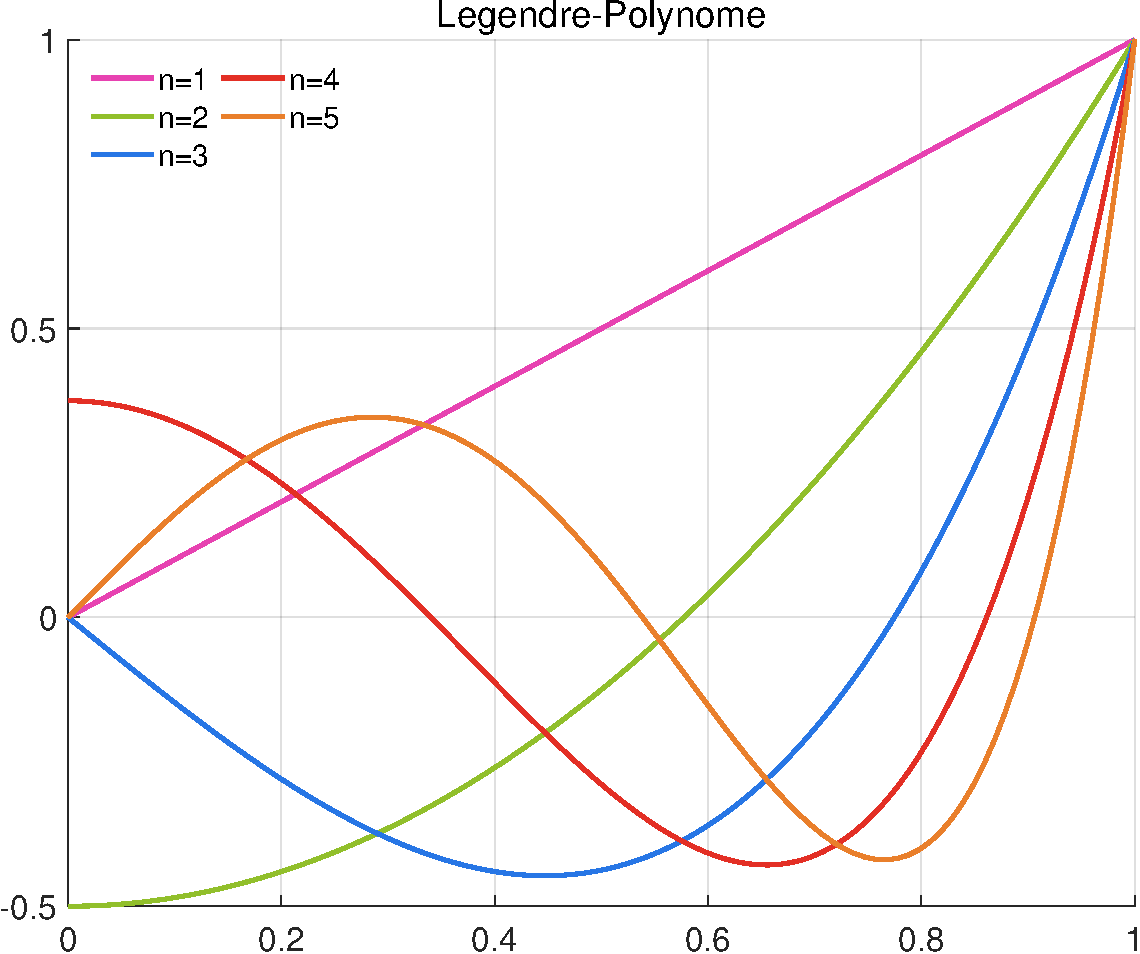
\includegraphics[width=\textwidth]{LegendrePolynome.pdf} 
	\caption[Legendre-Polynome.]{Legendre-Polynome $n=0\,\ldots n=6$.}
	\label{abb:solman_legpoly}
\end{figure}

Alternativ k�nnen die Legendre-Polynome �ber die \textbf{Rodrigues-Formel}

\begin{align}
    \PL n \lk x\rk = \frac{1}{2^n\,n!}\,\frac{\D^2}{\D\,x^2}\,\lk\lk x^2-1\rk^2\rk
\end{align}
berechnet werden oder �ber die \textbf{Integraldarstellung}

\begin{align}
    \PL n \lk x\rk = \frac{1}{\pi}\,\int\limits_0^\pi \lk x+\sqrt{x^2-1}\,\cos\varphi\rk^n\,\D\varphi \,.
\end{align}

F�r die Legendre-Polynome gelten folgende \textbf{Rekursionsformeln}:
\begin{align*}
    \lk n+1\rk\,\PL {n+1} \lk x\rk &= \lk 2n+1\rk\,x\,\PL n \lk x\rk -n\,\PL {n-1} \lk x\rk  ~~~~ \lk n=1,2,\ldots;\PL 0=1;\PL1 = x\rk \\
    \lk x^2-1\rk\,\frac{\D}{\D x}\,\PL n \lk x\rk &= n\,x\,\PL n \lk x\rk -n\,\PL {n-1} \lk x\rk \,.
\end{align*}
Die erste rekursive Formel l�sst sich mittels der Substitution $n'=n+1$ in folgender, h�ufig zu findender Weise darstellen:
\begin{align}
    n\,\PL n \lk x\rk = \lk 2n-1\rk\,x\,\PL {n-1} \lk x\rk - \lk n-1\rk\,\PL {n-2} \lk x\rk ~~~~ \lk n=2,3,\ldots;\PL 0=1;\PL1 = x\rk \,.
\end{align}

\textbf{Vollst�ndiges Orthogonalsystem}\\

Die Legendre-Polynome bilden auf ein vollst�ndiges Orthogonalsystem, sie sind also ein Spezialfall von orthogonalen Polynomen. Normiert man diese, so bilden sie ein vollst�ndiges Orthogonalsystem. \\
Es gilt
\begin{align}
    \int\limits_{-1}^1 \PL n \lk x\rk\,\PL m \lk x\rk\,\D x = \frac{2}{2n+1}\,\delta_{nm}\,,
\end{align}
wobei $\delta_{nm}$ das Kronecker-Delta bezeichnet. Dabei bedeutet die Vollst�ndigkeit, dass sich jede Funktion $f$ nach Legendre-Polynomen \anf{entwickeln} l�sst:
\begin{align}
    f\lk x\rk = \sum\limits_{n=0}^\infty c_n\,\PL n \lk x\rk
\end{align}
mit den Entwicklungskoeffizienten
\begin{align}
    c_n = \frac{2n+1}{2}\int\limits_{-1}^1 f(x)\,\PL n \lk x\rk\,\D x \,.
\end{align}


\subsection {Hermitesche Polynome} \label{kap:solman_HermitePoly}


\section{N�tzliche Integrale}

\begin{align}
\int x^2\,\sqrt{c^2-x^2} = \frac{x\,\lk c^2-x^2\rk^{3/2}}{4}+ \frac{c^2\,x\,\sqrt{c^2-x^2}}{8} + \frac{c^4}{8}\,\arcsin\frac{x}{c} \,.
\end{align}\\

\begin{align}
\int \frac{\D u}{\sqrt{b^2-u^2}} = \arcsin\frac{x}{c} \,.
\end{align} \\

\begin{align}
\int \frac{\D x}{\lk x^2+a^2\rk^m} = \frac{x}{2\,\lk m-1\rk\,a^2\lk x^2+a^2\rk^{m-1}} + \frac{2m-3}{\lk 2m-2\rk\,a^2}\,\int \frac{\D x}{\lk x^2+a^2\rk^{m-1}} \,.
\end{align}\\

\begin{align}
\int \lk ax+b\rk^{m/2}\,\D x = \frac{2\,\lk ax+b\rk^{\lk m+2\rk/2}}{\lk m+2\rk\, a} \,.
\end{align} \\

\begin{align}
\int x\,\lk ax+b\rk^{m/2}\D x = \frac{2\,\lk ax+b\rk^{\lk m+4\rk/2}}{\lk m+4\rk\, a^2} - \frac{2b\,\lk ax+b\rk^{\lk m+2\rk/2}}{\lk m+2\rk\, a^2} \,.
\end{align}

\subsection{Numerische Integration}

\textbf{Rechteckregel}
\begin{align}
\int\limits_a^b f\lk x\rk \D x\approx h \Big\{f\lk x_1\rk+f\lk x_2\rk+f\lk x_3\rk+\ldots +f\lk x_{N-1}\rk\Big\} \,,
\end{align}\\

wo $x_\text{i} = a+\lk i-1\rk\,h$, f�r $1\leq i \leq N$, $h=\lk h-a\rk / \lk N-1\rk$. \\

\textbf{Trapezregel}
\begin{align}
\int\limits_a^b f\lk x\rk \D x\approx \frac{h}{2}\Big\{f\lk x_1\rk+2\,\lek f\lk x_2\rk + f\lk x_3\rk + \ldots +f\lk x_{N-1}\rk\rek + f\lk x_\text{N}\rk\big\}\,,
\end{align}\\

wo die ganze Zahl $N\geq 2$, $x_\text{i} = a+\lk i-1\rk\, h$ f�r $1\leq i\leq N$, und $h \equiv \lk b-a\rk/\lk N-1\rk$.\\

\textbf{Simpson's Regel}
\begin{align}
\int\limits_a^b f\lk x\rk \D x\approx \frac{h}{3}\left\{\begin{array}{rcl} f\lk x_1\rk+2\,\lek f\lk x_2\rk + f\lk x_4\rk + f\lk x_6\rk + \ldots +f\lk x_{N-1}\rk\rek \\+4\,\lek f\lk x_3\rk + f\lk x_5\rk + f\lk x_7\rk + \ldots +f\lk x_{N-2}\rk\rek+ f\lk x_\text{N}\rk\end{array}\right\}\,,
\end{align}\\

wo $N\geq 3$ eine ungerade ganze Zahl ist, $x_\text{i} = a+\lk i-1\rk\,h$ f�r $1\leq i\leq N$, und $h \equiv \lk b-a\rk/\lk N-1\rk$.

\section{Funktionentheorie}

Cauchy-Riemann'sche Differenzialgleichungen:
\begin{align}
    f\lk z\rk = u\lk x+\im\,y\rk + \im\,v\lk x+\im\,y\rk: ~~~~ u_\text{x} = v_\text{y}, ~~~~ u_\text{y} = -v_\text{x} \,.
\end{align}
Residuensatz:
\begin{align}
    \oint f\lk z\rk \D z = 2\pi\,\im\,\sum\limits_{j=1}^n\,\res_\text{zj}\,f\lk z\rk \,.
\end{align}
Residuum bei einer einfachen Polstelle:
\begin{align}
    \res_{z_0}\,f\lk z\rk =  \lim_{z\to z_0}\lk z-z_0\rk\,f\lk z\rk \,.
\end{align}

 
%
%\clearpage
%%\documentclass[makeidx,envcountchap,graybox,deutsch,ngerman,sectrefs]{svmono}
%\documentclass[envcountchap,graybox,deutsch,sectrefs]{svmono}
%%%%% eigene tempor�re Abk�rzungsliste, f�r die Zeit, bis einheitliche Schreibungen bestehen
\usepackage{tempshort}
%%  Von Springer empfohlene Pakete %% 
%%\documentclass[envcountsect,graybox,deutsch,sectrefs]{svmono}
\usepackage{chapterbib}
\usepackage{type1cm}
\usepackage[ansinew]{inputenc}
\usepackage{babel}
\usepackage[pdftex]{graphicx} %PDF-Vektorgrafiken einbinden
\usepackage{newtxtext} %Typischer Springer-Font
\usepackage{newtxmath}
\usepackage{multicol}
\usepackage[bottom]{footmisc} %Platziert alle Fu�noten unten  
\usepackage[nobreak]{cite}
%\usepackage{biblatex}
\usepackage{cancel}
\usepackage[absolute]{textpos}
\usepackage{graphicx}
\usepackage{pdfpages}

%\usepackage{floatrow}
%\usepackage{mwe}
\usepackage[figuresright]{rotating}
\usepackage{bigints}
\let\laplace\relax  % Vermeidung der Fehlermeldung "\laplace already defined."
\usepackage{trfsigns}
\usepackage{amsmath}
\usepackage{tabulary}
\usepackage{tabularx}

%%  Eigene Pakete %%
\usepackage{adjustbox}
\usepackage{wasysym}
\usepackage{gensymb}
\usepackage{float}
\usepackage{caption}
\usepackage[left=5cm,right=4cm,top=3cm,bottom=4cm,includeheadfoot]{geometry}

%\usepackage{wasysym}
%\usepackage{bigints}
%\usepackage{esint}
%\usepackage{relsize,exscale}

\usepackage{mathtools}   % Vermeidung der Fehlermeldung "Undefined control sequence \coloneqq."


% header and footer
\usepackage{fancyhdr}
\pagestyle{fancy}
\fancyhead[LE,RO]\thepage
\renewcommand{\sectionmark}[1]{\markright{\thesection.\ #1}}
%\fancyhead[LO]{\nouppercase\leftmark}
%\fancyhead[RE]{\nouppercase\rightmark}
\fancyhead[LO]{\nouppercase\rightmark}
\fancyhead[RE]{\nouppercase\leftmark}
\fancyfoot{}
% svmono hat offenbar irgendwas merkw�rdig definiert, darum mu� hier verbreitert werden
%\addtolength\headwidth{25pt}
\setlength{\headheight}{25pt}

%% Units
\usepackage{siunitx}
\sisetup{
  locale = US,
  per-mode = reciprocal, %symbol, % | reciprocal | fraction | ?
  exponent-product = \cdot,
  separate-uncertainty,
  %exponent-to-prefix,
  %prefixes-as-symbols = false,
  %list-units = brackets,% | single | repeat
  %range-units = brackets,% | single | repeat
  %multi-part-units = brackets,% | single | repeat
}
\usepackage{chngcntr}
\usepackage{booktabs}
\usepackage{slashed}
\usepackage{listings}
\usepackage{color} %red, green, blue, yellow, cyan, magenta, black, white
%\usepackage{color} %Einfache Farbendefinition -> von Graybox-Option ben�tigt
\usepackage{multirow}
\usepackage{longtable} %Tabellen �ber mehrere Seiten hinweg
\usepackage{framed} % von Graybox-Option ben�tigt
\usepackage[shortlabels]{enumitem} %Erweiterte Aufz�hloptionen
\usepackage{array}
\usepackage[xindy]{imakeidx} %Wortindex und Personenindex erstellen

\usepackage[hyphens]{url}
%\usepackage[breaklinks,colorlinks=true,linkcolor=black,urlcolor=blue,citecolor=black,filecolor=green,hyperfootnotes=false]{hyperref}
\usepackage[                                    %Hyperref erstellt ein Bookmark/Lesezeichen im PDF. siehe https://www.namsu.de/Extra/pakete/Hyperref.html
bookmarksopen=true,															%Das Lesezeichen ist ge�ffnet beim �ffnen der PDF.
bookmarksnumbered=true,                         %Zahlen werden im Bookmark angezeigt.   
plainpages=false,
pdfpagelabels,
colorlinks=true,                                %Links werden farbig dargestellt.
linkcolor=black, citecolor=black, urlcolor=cyan %Farben definieren.
]{hyperref}                                     %Sollte als letztes eingebunden werden, da es sehr viele Verweise und �nderungen erzeugt. Das Packet ist sehr stark, aber auch umfangreich ist. 

%\usepackage[breaklinks,colorlinks=true,linkcolor=black,urlcolor=blue,citecolor=black,filecolor=green,hyperfootnotes=false]{hyperref}
%\usepackage[breaklinks,colorlinks=true,linkcolor=black,urlcolor=blue,citecolor=black,filecolor=green,hyperfootnotes=false
            %pdftex,
            %pdfauthor={Kaschke, Cartarius},
            %pdftitle={Finger�bungen der Physik}
            %pdfsubject={Ein Repetitorium und �bungsbuch zu im Studium wenig behandelten Kapiteln der Physik mit ausf�hrlich behandelten Problemen und MATLAB-Programmen},
            %pdfkeywords={Physik, Mechanik}
            %]{hyperref}
\pdfminorversion=5

\usepackage{hypcap}
\usepackage[record,section=section,stylemods={mcols},automake]{glossaries-extra}
\usepackage{glossary-longextra}
%\usepackage{glossary-bookindex}
%\makeindex
\setglossarystyle{long-name-sym-desc-loc}
\setabbreviationstyle[acronym]{long-short}

\definecolor{killA}{rgb}{.7,.3,.3}
\newcommand\killA[1]{\bgroup\color{killA}{\cancel{#1}}\egroup}
\newcommand\killB[1]{\bgroup\color{cyan!30!black}{\cancel{#1}}\egroup}

% typographisch korrekte Abk�rzungen (needs to be loaded after hyperref)
\usepackage{abbrev}
\newglossary*{bew}{Glossar}
\newglossary*{hm}{Glossar}
\newglossary*{adyn}{Glossar}
\newglossary*{kontmech}{Glossar}
\newglossary*{aero}{Glossar}
\newglossary*{edyn}{Glossar}
\newglossary*{spo}{Glossar}
\newglossary*{optbas}{Glossar}
\newglossary*{optger}{Glossar}
\newglossary*{optatm}{Glossar}
\newglossary*{optspez}{Glossar}
\GlsXtrLoadResources[src={bew/gloss},type=bew]
\GlsXtrLoadResources[src={hm/gloss},type=hm]
\GlsXtrLoadResources[src={adyn/gloss},type=adyn]
\GlsXtrLoadResources[src={kontmech/gloss},type=kontmech]
\GlsXtrLoadResources[src={aero/gloss},type=aero]
\GlsXtrLoadResources[src={spo/gloss},type=spo]
\GlsXtrLoadResources[src={edyn/gloss},type=edyn]
\GlsXtrLoadResources[src={optbas/gloss},type=optbas]
\GlsXtrLoadResources[src={optger/gloss},type=optger]
\GlsXtrLoadResources[src={optatm/gloss},type=optatm]
\GlsXtrLoadResources[src={optspez/gloss},type=optspez]
\glssetcategoryattribute{bew}{indexname}{true}
%\renewcommand\index\newterm
%\newcolumntype{g}[1]{>{\RaggedRight\hspace{0pt}}p{#1}}
%\renewcommand\glslongextraNameAlign{g}
\renewcommand\glslongextraLocationAlign{@{\ ~\ }>{\raggedright}p{\glspagelistwidth}}
\definecolor{gls}{rgb}{.4,.4,.5}
\renewcommand*{\glstextformat}[1]{\textcolor{gls}{#1}}

%Absatzregeln
\clubpenalty = 30000 %Keine einzelnen Absatzzeilen
\widowpenalty = 30000
\setlength{\parindent}{0em} 
\newcolumntype{L}[1]{>{\raggedright\arraybackslash}p{#1}}
\newcolumntype{C}[1]{>{\centering\arraybackslash}p{#1}}
\newcolumntype{R}[1]{>{\raggedleft\arraybackslash}p{#1}}

\usepackage{xstring}

\newcommand\mfile[2]{%
\saveexpandmode\noexpandarg
\StrSubstitute{#2}{_}{\_}[\tmpname]
\restoreexpandmode
\href{MatlabDateien/\chapname/#1\tmpname}{\tmpname}}

%%% Hyperlinks zu MATLAB Dateien
%\newcommand\mlref[1]{\mfile{}{#1}}
%\newcommand\mlinclref[1]{\mfile{IncludeFolder/}{#1}}
%\newcommand\mldataref[1]{\mfile{Data/}{#1}}

%%% .. f�r ein Verzeichnis hoch
%%% . f�r aktuelle Verzeichnis
%% lokal: MatlabDateien/bew
%\newcommand\mlbewref[1]{\href{MatlabDateien/bew/#1}{#1}}
%% git: https://github.com/sn-code-inside/fingeruebungen-physik/tree/main/bew

\newcommand{\mlrefwithindex}[2]{%
  \index[mfiles]{#2}%   <-- Eintrag im M-File-Index mit aktueller Seitenzahl
  \href{https://github.com/sn-code-inside/fingeruebungen-physik/tree/main/#1/#2}{#2}%
}


%\newcommand\mlbewref[1]{\href{https://github.com/sn-code-inside/fingeruebungen-physik/tree/main/bew/#1}{#1}}
%\newcommand\mlbewdref[1]{\href{https://github.com/sn-code-inside/fingeruebungen-physik/tree/main/bew/Data/#1}{#1}}
%\newcommand\mlbewiref[1]{\href{https://github.com/sn-code-inside/fingeruebungen-physik/tree/main/bew/IncludeFolder/#1}{#1}}
%\newcommand\mlkontmechref[1]{\href{https://github.com/sn-code-inside/fingeruebungen-physik/tree/main/kontmech/#1}{#1}}
%\newcommand\mlkontmechdref[1]{\href{https://github.com/sn-code-inside/fingeruebungen-physik/tree/main/kontmech/Data/#1}{#1}}
%\newcommand\mlkontmechiref[1]{\href{https://github.com/sn-code-inside/fingeruebungen-physik/tree/main/kontmech/IncludeFolder/#1}{#1}}
%\newcommand\mlhmref[1]{\href{https://github.com/sn-code-inside/fingeruebungen-physik/tree/main/hm/#1}{#1}}
%\newcommand\mlhmdref[1]{\href{https://github.com/sn-code-inside/fingeruebungen-physik/tree/main/hm/Data/#1}{#1}}
%\newcommand\mlhmiref[1]{\href{https://github.com/sn-code-inside/fingeruebungen-physik/tree/main/hm/IncludeFolder/#1}{#1}}
%\newcommand\mladynref[1]{\href{https://github.com/sn-code-inside/fingeruebungen-physik/tree/main/adyn/#1}{#1}}
%\newcommand\mladyndref[1]{\href{https://github.com/sn-code-inside/fingeruebungen-physik/tree/main/adyn/Data/#1}{#1}}
%\newcommand\mladyniref[1]{\href{https://github.com/sn-code-inside/fingeruebungen-physik/tree/main/adyn/IncludeFolder/#1}{#1}}
%\newcommand\mledynref[1]{\href{https://github.com/sn-code-inside/fingeruebungen-physik/tree/main/edyn/#1}{#1}}
%\newcommand\mledyndref[1]{\href{https://github.com/sn-code-inside/fingeruebungen-physik/tree/main/edyn/Data/#1}{#1}}
%\newcommand\mledyniref[1]{\href{https://github.com/sn-code-inside/fingeruebungen-physik/tree/main/edyn/IncludeFolder/#1}{#1}}
%\newcommand\mloptbasref[1]{\href{https://github.com/sn-code-inside/fingeruebungen-physik/tree/main/optbas/#1}{#1}}
%\newcommand\mloptbasdref[1]{\href{https://github.com/sn-code-inside/fingeruebungen-physik/tree/main/optbas/Data/#1}{#1}}
%\newcommand\mloptbasiref[1]{\href{https://github.com/sn-code-inside/fingeruebungen-physik/tree/main/optbas/IncludeFolder/#1}{#1}}
%\newcommand\mloptspezref[1]{\href{https://github.com/sn-code-inside/fingeruebungen-physik/tree/main/optspez/#1}{#1}}
%\newcommand\mloptspezdref[1]{\href{https://github.com/sn-code-inside/fingeruebungen-physik/tree/main/optspez/Data/#1}{#1}}
%\newcommand\mloptspeziref[1]{\href{https://github.com/sn-code-inside/fingeruebungen-physik/tree/main/optspez/IncludeFolder/#1}{#1}}

\newcommand\mlbewref[1]{\mlrefwithindex{bew}{#1}}
\newcommand\mlbewdref[1]{\mlrefwithindex{bew/Data}{#1}}
\newcommand\mlbewiref[1]{\mlrefwithindex{bew/Include}{#1}}
\newcommand\mlkontmechref[1]{\mlrefwithindex{kontmech}{#1}}
\newcommand\mlkontmechdref[1]{\mlrefwithindex{kontmech/Data}{#1}}
\newcommand\mlkontmechiref[1]{\mlrefwithindex{kontmech/Include}{#1}}
\newcommand\mlhmref[1]{\mlrefwithindex{hm}{#1}}
\newcommand\mlhmdref[1]{\mlrefwithindex{hm/Data}{#1}}
\newcommand\mlhmiref[1]{\mlrefwithindex{hm/Include}{#1}}
\newcommand\mladynref[1]{\mlrefwithindex{adyn}{#1}}
\newcommand\mladyndref[1]{\mlrefwithindex{adyn/Data}{#1}}
\newcommand\mladyniref[1]{\mlrefwithindex{adyn/Index}{#1}}
\newcommand\mledynref[1]{\mlrefwithindex{edyn}{#1}}
\newcommand\mledyndref[1]{\mlrefwithindex{edyn/Data}{#1}}
\newcommand\mledyniref[1]{\mlrefwithindex{edyn/Index}{#1}}
\newcommand\mloptbasref[1]{\mlrefwithindex{optbas}{#1}}
\newcommand\mloptbasdref[1]{\mlrefwithindex{optbas/Data}{#1}}
\newcommand\mloptbasiref[1]{\mlrefwithindex{optbas/Include}{#1}}
\newcommand\mloptspezref[1]{\mlrefwithindex{optspez}{#1}}
\newcommand\mloptspezdref[1]{\mlrefwithindex{optspez/Data}{#1}}
\newcommand\mloptspeziref[1]{\mlrefwithindex{optspez/Include}{#1}}
\newcommand\mloptgerref[1]{\mlrefwithindex{optger}{#1}}
\newcommand\mloptgerdref[1]{\mlrefwithindex{optger/Data}{#1}}
\newcommand\mloptgeriref[1]{\mlrefwithindex{optger/Include}{#1}}
\newcommand\mloptatmref[1]{\mlrefwithindex{optatm}{#1}}
\newcommand\mloptatmdref[1]{\mlrefwithindex{optatm/Data}{#1}}
\newcommand\mloptatmiref[1]{\mlrefwithindex{optatm/Include}{#1}}



\newcommand\mlcmd[1]{\textcolor{cyan}{\texttt{#1}}}

%Grafikregeln
\graphicspath{{hm/graphs/}
	                    	{bew/graphs/}
     						{kontmech/graphs/}
							{hm/graphs/}
							{adyn/graphs/}
							{edyn/graphs/}
							{kontmech/graphs/}
							{spo/graphs/}
							{optbas/graphs/}
							{optger/graphs/}
							{optatm/graphs/}
							{solman/graphs/}
                                                        {aero/graphs}}
\DeclareGraphicsExtensions{.pdf, .png, .jpg, .jpeg}
\def\figname{Abb}
\newcommand\figref[1]{\figname.\ \ref{abb:#1}}
\usepackage[labelfont=bf]{caption}

\usepackage{tocloft}
\usepackage{etoc}
\setlength\cftfignumwidth{30pt}

% Flatterrand links
\cftsetindents{chapter}{0em}{4em}
\cftsetindents{section}{1.5em}{4em}
\cftsetindents{subsection}{3.8em}{4em}

% flacher Rand links
%\cftsetindents{chapter}{0em}{4em}
%\cftsetindents{section}{0em}{4em}
%\cftsetindents{subsection}{0em}{4em}

\newcommand\partitle[1]{
\addcontentsline{toc}{part}{#1}
\begin{titlepage}
  %\vskip 60%\p@
  \begin{center}
    {\LARGE Finger�bungen der Physik -- #1 \par}
    \vskip 3em%
    {\large Michael Kaschke und Holger Cartarius\par}
  \end{center}
\end{titlepage}
}

%\newcommand\mlref[1]{\href{\chapname/matlab/#1}{#1}}
%\newcommand\mlinclref[1]{\href{\chapname/matlab/IncludeFolder/#1}{\color{cyan}{#1}}}

%Neue Kommandos
\newcommand{\lk}{\left(}        %gro�e runde Klammer (links)
\newcommand{\rk}{\right )}      %gro�e runde Klammer (rechts)
\newcommand{\lgk}{\left \{}     %gro�e geschweifte Klammer (links)
\newcommand{\rgk}{\right \}}    %gro�e geschweifte Klammer (rechts)
\newcommand{\lek}{\left [}      %gro�e eckige Klammer (links)
\newcommand{\rek}{\right ]}     %gro�e eckige Klammer (rechts)
\newcommand{\anf}[1]{\glqq#1\grqq}    %Deutsche Anf�hrungszeichen: \anf{}
\newcommand{\defined}{:=}				%Definition
\newcommand{\curl}{\text{\textbf{rot}}\,}	%Rotation-Operator curl()
\newcommand{\ket}[1]{|#1\rangle}		%Quantenmechanischer Zustand
\newcommand{\curvelintri}{\,\overset{\blacktriangle}{\smallfrown}}
\newcommand{\straighttri}{\blacktriangle}
\newcommand{\UT}{\text{UT}}
\newcommand{\UTC}{\text{UTC}}
\newcommand{\JD}{\text{JD}}
\newcommand{\JDE}{\text{JDE}}
\newcommand{\MJD}{\text{MJD}}
\newcommand{\TDT}{\text{TDT}}
\newcommand{\TT}{\text{TT}}
\newcommand{\NVS}{\text{Navier-Stokes-Gleichungen}}
\newcommand{\MWG}{\text{Maxwell-Gleichungen}}
\newcommand{\EMW}{\text{Elektromagnetische Wellen}}
\newcommand{\eMW}{\text{elektromagnetischen Wellen}}
\newcommand{\RT}{\text{Relativit�tstheorie~}}
\newcommand{\au}{\mathrm{AE}}
\newcommand{\ET}{\text{ET}}
\newcommand{\TAI}{\text{TAI}}
\newcommand{\GMST}{\text{GMST}}
\newcommand{\LMST}{\text{LMST}}
\newcommand{\MESZ}{\text{MESZ}}
\newcommand{\KOS}{\text{Koordinatensystem }}
\newcommand{\DGL}{\text{Differentialgleichung }}
\newcommand{\NA}{\text{NA}}
\newcommand{\uA}{\text{u}}  %atomare Masseneinheit
\newcommand{\MOZ}{\text{MOZ}}
\newcommand{\grad}{\text{\textbf{grad}}\,}	%Gradient-Operator grad()
\newcommand{\uproman}[1]{\mathrm{\uppercase\expandafter{\romannumeral#1}}}
\newcommand{\lowroman}[1]{\romannumeral#1\relax}

\newcommand\todo[1]{\textcolor{red}{TODO: #1}}

\renewcommand{\=}[1]{\stackrel{\text{#1}}{=}}  %Schrift �ber Gleich-Zeichen
\renewcommand{\d}{\partial}
\newcommand{\lra}{\Leftrightarrow}  %�quivalenz-Pfeile
\newcommand{\abs}[1]{\left\vert#1\right\vert}     %Betragsklammern
\renewcommand{\Re}{\mathrm{Re}}                          %Realteil
\renewcommand{\Im}{\mathrm{Im}}                          %Imagin�rteil
\renewcommand{\im}{\mathrm{i}}                         %Imagin�re Einheit
\renewcommand{\epsilon}{\varepsilon} 
\newcommand{\keff}{k_\text{eff}}
\newcommand{\con}{\text{const}}
\newcommand{\conv}{\vec{const}}
\newcommand{\PL}{\mathcal{P}_}
\newcommand{\artanh}{\mathrm{artanh}}
% QED-Symbol im text- bzw. Mathemodus
\newcommand{\textqed}{\hfill ~ $\square$}
\newcommand{\mmqed}{\tag*{$\square$}}

\newcommand{\fa}{(\textbf{a}) }
\newcommand{\fb}{(\textbf{b}) }
\newcommand{\fc}{(\textbf{c}) }
\newcommand{\fd}{(\textbf{d}) }
\newcommand{\fe}{(\textbf{e}) }
\newcommand{\ff}{(\textbf{f}) }

\newcommand{\iF}{im Folgenden~}
\newcommand{\iA}{im Allgemeinen~}


\DeclareMathOperator\divv{div}
\DeclareMathOperator\res{Res}
\DeclareMathOperator{\sech}{sech}
\DeclareMathOperator\sgn{sgn}

% f�r Appendix - MATLAB Referenz
\newcommand{\rotv}{\vec{rot}\,}
\newcommand{\gradv}{\vec{grad}\,}
\newcommand{\nablav}{\vec{\nabla}\,}

\newcommand{\ceil}{\mathrm{ceil}}
\newcommand{\sinc}{\mathrm{sinc}}
\newcommand{\diag}{\mathrm{diag}}
\newcommand{\sign}{\mathrm{sign}}
\newcommand{\length}{\mathrm{length}}
\newcommand{\sort}{\mathrm{sort}}
\newcommand{\summ}{\mathrm{sum}}
\newcommand{\asin}{\mathrm{asin}}
\newcommand{\acos}{\mathrm{acos}}
\newcommand{\atan}{\mathrm{atan}}
\newcommand{\prodd}{\mathrm{prod}}
\newcommand{\median}{\mathrm{mediab}}
\newcommand{\mean}{\mathrm{mean}}
\newcommand{\std}{\mathrm{std}}
\newcommand{\eye}{\mathrm{eye}}
\newcommand{\zeros}{\mathrm{zeros}}
\newcommand{\ones}{\mathrm{ones}}
\newcommand{\rand}{\mathrm{rand}}
\newcommand{\inline}{\mathrm{inline}}
\newcommand{\modd}{\mathrm{mod}}
\newcommand{\floor}{\mathrm{floor}}
\newcommand{\round}{\mathrm{round}}
\newcommand{\rem}{\mathrm{rem}}
\newcommand{\sqrtt}{\mathrm{sqrt}}
\newcommand{\triu}{\mathrm{triu}}
\newcommand{\tril}{\mathrm{tril}}
\newcommand{\size}{\mathrm{size}}
\newcommand{\dett}{\mathrm{det}}
\newcommand{\inv}{\mathrm{inv}}
\newcommand{\rank}{\mathrm{rank}}
\newcommand{\rref}{\mathrm{rref}}
\newcommand{\eig}{\mathrm{eig}}
\newcommand{\poly}{\mathrm{poly}}
\newcommand{\lu}{\mathrm{lu}}
\newcommand{\qr}{\mathrm{qr}}
\newcommand{\quaddd}{\mathrm{quad}}
\newcommand{\fzero}{\mathrm{fzero}}
\newcommand{\roots}{\mathrm{roots}}
\newcommand{\odezd}{\textcolor{mygreen}{\texttt{ode23}}}
\newcommand{\odevf}{\textcolor{mygreen}{\texttt{ode45}}}
\newcommand{\odeeds}{\textcolor{mygreen}{\texttt{ode13s}}}
\newcommand{\odeefs}{\textcolor{mygreen}{\texttt{ode15s}}}
\newcommand{\ddezd}{\textcolor{mygreen}{\texttt{dde23}}}
\newcommand{\onlineZ}{online verf�gbaren Zusatzmaterialien{}}
\newcommand{\MKc}{\url{https://www.fingeruebungen-physik.de}{}}
\newcommand{\linklsg}{\href{https://www.fingeruebungen-physik.de}{\textcolor{blue} {$\rightarrow$ L�sungsteil.}}}
\newcommand{\githubSN}{\url{https://github.com/sn-code-inside/fingeruebungen-physik}{}\,\,}

\newcommand{\FT}{\mathcal{F}} %Fourier-Transformierte

% Aufz�hlung der L�sungen der Teilaufgaben
\newlist{subprobs}{enumerate}{1}
\setlist[subprobs]{
  label= \textbf{\textit{Teilaufgabe}} \textbf{\textit{\arabic*:}} \protect\thissubprob,
  ref=\arabic*, itemsep=\baselineskip, align=left}
\newcommand{\subprob}[1]{
  \def\thissubprob{\textbf{\textit{#1}}}\item ~\vspace{0.2\baselineskip} \newline}

\renewenvironment{example}[1]{
\refstepcounter{example}\par\medskip
\begin{shaded} 
\begin{samepage}
\noindent \textbf{\textit{Beispiel~\theexample: {#1}}}\\ 
\noindent{\color{black} \rule{\textwidth}{0.2 mm}}
\end{samepage}
}{\end{shaded}
\noindent{\color{black} \rule{\textwidth}{0.2 mm}}
} % or snugshade
\definecolor{shadecolor}{gray}{0.95}
\definecolor{mygreen}{RGB}{28,172,0} % color values Red, Green, Blue
\definecolor{mylilas}{RGB}{170,55,241}

\newenvironment{infobox}[1]{
     \begin{shaded} 
     \begin{samepage}
\noindent{\color{black} \rule{\textwidth}{0.2 mm}}
     \end{samepage}
}{\end{shaded}
\noindent{\color{black} \rule{\textwidth}{0.2 mm}}
} 
\definecolor{shadecolor}{gray}{0.95}
\definecolor{mygreen}{RGB}{28,172,0} % color values Red, Green, Blue
\definecolor{mylilas}{RGB}{170,55,241}


\newenvironment{nebenrechnung}[1]{
\begin{shaded} 
\begin{samepage}
\noindent\textbf{Nebenrechnung: \\} 
\noindent{\color{black} \rule{0.1\columnwidth}{0.2mm} \\}
\end{samepage}
}{\end{shaded}
\noindent{\color{black} \rule{0.1\columnwidth}{0.2mm} \\}
} % or snugshade
\definecolor{shadecolor}{gray}{0.95}
\definecolor{mygreen}{RGB}{28,172,0} % color values Red, Green, Blue
\definecolor{mylilas}{RGB}{170,55,241}

\newenvironment{merksatz}[1]{
\begin{shaded} 
\begin{samepage}
\noindent\textbf{Merke:\\} 
\noindent{\color{black} \rule{0.9\columnwidth}{0.2mm} \\ \\}
\end{samepage}
}{\end{shaded}
\noindent{\color{black} \rule{0.9\columnwidth}{0.2mm} \\}
} % or snugshade


\lstset{language=Matlab,%
    %basicstyle=\color{red},
    %basicstyle={\linespread{0.9}\ttfamily},
    basicstyle=\footnotesize\ttfamily,
    breaklines=true,%
    morekeywords={matlab2tikz},
    keywordstyle={\small \color{mygreen}},%
    morekeywords=[2]{1}, keywordstyle=[2]{\small\color{black}},
    identifierstyle={\small \color{black}},%
    stringstyle={\small\color{mylilas}},
    commentstyle={\small\color{mylilas}},%
    showstringspaces=false,%without this there will be a symbol in the places where there is a space
    numbers=left,%
    numberstyle={\tiny \color{black}},% size of the numbers
    numbersep=9pt, % this defines how far the numbers are from the text
    emph=[1]{for,end,else,break, function},emphstyle=[1]\small \color{blue}, %some words to emphasise
    emph=[2]{odeset},emphstyle=[2]\small \color{mygreen}, %some words to emphasise
    %emph=[2]{word1,word2}, emphstyle=[2]{style},    
}

%\bibliographystyle{spphys.bst}

%Trennregeln f�r spezielle Worte
%\hyphenation{Fresnel \matlab �qui-nok-ti-um}

\DeclareSIUnit\erg{erg}
\DeclareSIUnit\cal{cal}
\DeclareSIUnit\celsius{C}
\DeclareSIUnit\m{M}
\DeclareSIUnit\kel{K^{-4}}

%Stichwort- und Personenverzeichnis
\makeindex[title=Stichwortverzeichnis] % Create the default index
\makeindex[name=personen,title=Personenverzeichnis] % Create an index named 'personen'
\newcommand{\indexp}[1]{\index[personen]{#1}}
\makeindex[name=mfiles,title=MATLAB-Skriptverzeichnis,columns=2]

% list of exercises
\newcommand{\loxname}{\Large �bungsverzeichnis}  % einheitliche Gr��e Large
\newlistof[chapter]{prob}{lox}\loxname
\newcommand\uebung[3][]{\label{prob:#2}%
\addcontentsline{lox}{prob}{\protect\numberline{}{\probRef{#2}:~#3#1}}%
\textbf{#1#3}\\[\baselineskip]}
\makeatletter
\renewcommand{\l@prob}{\@dottedtocline{1}{0em}{0em}}
\makeatother

\newcommand\einfach{\uebung[~$\ast$~~]}
\newcommand\mittel{\uebung[~$\ast\,\ast$~~]}
\newcommand\schwierig{\uebung[~$\ast\,\ast\,\ast$~~]}
\newcommand\zusatz{\uebung[~$\ast\,\ast\,\ast\,!$~~]}
%\newcommand\einfach{\uebung[~\textbf{*}~~]}
%\newcommand\mittel{\uebung[~\textbf{*\,*}~~]}
%\newcommand\schwierig{\uebung[~\textbf{*\,*\,*}~]}
%\newcommand\zusatz{\uebung[~\textbf{*\,*\,*\,!}~~]}
\usepackage[atend]{bookmark}
%\BookmarkAtEnd{%
%\bookmarksetup{startatroot}\bookmark[level=0,named=\loxname]{}}

\newcommand\kapitel[1]{Kapitel \ref{kap:#1}}
%\newcommand\kap[1]{Kap.\ \ref{kap:#1}}
\newcommand\kap[1]{Kap. \ref{kap:#1}}

\begin{document}
% customize prob and sol in svmono
\makeatletter
%\counterwithin*{chapter}{part}

\spn@wtheorem{prob}{\bgroup\exercisename\egroup}{\bfseries}{\rmfamily}
\makeatother
\renewenvironment{sol}[1]{\par\addvspace{6pt}\noindent\phantomsection{\textbf{L�sung \ref{#1}}} \ignorespaces}{\par\addvspace{6pt}}
\newcommand\probRef[1]{�bung \ref{prob:#1}}
\renewcommand\probref[1]{\textbf{\probRef{#1}}}
\newcommand\lsgref[1]{L�sung \ref{lsg:#1}}

\newcommand\sbullet[1][.5]{\mathbin{\vcenter{\hbox{\scalebox{#1}{$\bullet$}}}}}

\setcounter{table}{0}


%%%%%%%%%%%%%%%%%%%%%%%%%%%%%%%%%%%%%%%%%%%%%%%%%%%%%%%%%%%%%

\chapter{\matlab-Basics} \label{kap:solman_matlab}

Im Folgenden sollen einige \matlab-Elemente und -Funktionalit�ten vorgestellt werden. Es geht hierbei nicht darum, eine Vorlesungsskript oder gar ein kurzgefasstes Lehrbuch f�r \matlab{} zusammenzustellen. Dazu gibt es viele hervorragende Standardwerke (\zb \cite{Wilson2003, Pietruszka2020, Schweizer2016, Attaway2013}) und auch umfangreiche Online-Dokumentationen im Internet (\zb \url{https://www.mathworks.com/matlabcentral}). Wir wollen mit der Zusammenstellung die Themen herausheben, die in der Computational Physics (CP) h�ufig vorkommen.


\section{Matrix-Operationen}
Wie im Namen hinterlegt - MATrix LABoratory - verwendet \matlab{} f�r Variablen konsequent und komfortable die Matrixschreibweise. Umrahmt von eckigen Klammern k�nnen die Zeilen einer Matrix getrennt durch ein Semikolon hintereinander eingegeben werden.
\begin{lstlisting} [frame=single]
>> x = [1 2 3;4 3 2]
x =
     1     2     3
     4     3     2
\end{lstlisting} 
Sub-Matrizen sind �ber die Angabe von Zeilen- und Spaltenindices adressierbar, hier \zb die Selektion von Zeile 1 und Spalten 2 bis Ende der Matrix $x$.
\begin{lstlisting} [frame=single]
>> x(1,2:end)
ans =
    2    3
\end{lstlisting} 
Matrixoperationen, \zb $x\cdot x^T$, folgen konsequent den Gesetzen der linearen Algebra, man achte selber auf korrekte Zeilen- und Spaltendimensionen. Ein angeh�ngter Apostroph transponiert die Matrix.
\begin{lstlisting} [frame=single]
>> x*x'
ans =
    14    16
    16    29
\end{lstlisting} 
Die M�glichkeit zur elementweisen Multiplikation hingegen bietet der Punkt-Operator.
\begin{lstlisting} [frame=single]
>> x.*x
ans =
     1     4     9
    16     9     4
\end{lstlisting} 
Zahlreiche mathematische Funktionen (\mlcmd{sin}, \mlcmd{cos}, \mlcmd{exp},...) gestatten in der Regel matrixwertige Argumente und liefern elementweise Funktionswerte, der skalare Fall entspricht dem Sonderfall der Matrixdimension $1\times 1$. 
Weitere \matlab-Funktionen wie \zb \mlcmd{max}, \mlcmd{min}, \mlcmd{mean}  agieren an Zeilen- oder Spaltenvektoren, w�hrend sich die Funktionsweise anderer Matrixfunktionen wie beispielsweise \mlcmd{inv}, \mlcmd{norm}, \mlcmd{eig} aus deren Kontext heraus ergibt.
�u�erst praktisch ist der Einsatz vektorwertiger Variablen bei Zeitreihen, die bei geschickten Einsatz sehr effektiv verwendet werden k�nnen und in geeigneter Matrixnotation \ggf ohne Schleifenfunktionen auskommen k�nnen.

%-----------------------------------------------------------------------------------------------------------------------------------------------------------------------------
%\section{Ein- und Ausgabe} \label{kap:solman_matlab_IO}
\section{Import aus externen Datenquellen}

\matlab{} bietet vielf�ltige Unterst�tzung beim Import von externen Daten. Neben Datenbankanbindungen, auf die hier nicht eingegangen werden soll, sind  kommaseparierte Textdateien h�ufig die Quelle externen Zahlenmaterials. Mehrere M�glichkeiten zum Datenimport bestehen, so lassen sich z.B. Einzelwerte aus \mlbewdref{Liste.csv} mittels \mlcmd{csvread} unmittelbar einer Variable~\mlcmd{Liste} zuweisen:
\begin{lstlisting} [frame=single]
>> type Liste.csv
2,3

>> Liste = csvread('Liste.csv')

Liste =
     2     3
\end{lstlisting} 

Etwas komplexere Datenstrukturen, z.B. bestehend aus mehreren Datentypen (string, integer, float) wie in \mlbewdref{TypListe.csv}, lassen sich unter Ber�cksichtigung ihrer Struktur mittels \mlcmd{textscan} einlesen und einer matrixwertigen Variable \mlcmd{ListeArray} zuweisen:
\begin{lstlisting} [frame=single]
>> type TypListe.csv
'r' 1 0 0 0.2
'g' 0 1 0 0.3
'b' 0 0 1 0.4

>> fileID = fopen('TypListe.csv','r');
>> ListeArray = textscan(fileID,'%s%u%u%u%f');
>> fclose(fileID);
>> ListeArray{5}
ans =
    0.2000
    0.3000
    0.4000
\end{lstlisting} 

%\newpage
Ist das Zielformat wie bei \mlbewdref{PlanetenFarben.csv} eine Tabelle, so bietet sich die Verwendung des \mlcmd{readtable}-Befehls an:
\begin{lstlisting} [frame=single]
>> Colors = readtable('PlanetenFarben.csv');
Colors =
 15x9 table
R       G       B       Name         Farbe            Hex       
______  ______  ______  ___________  _______________  __________...
0.9059  0.2588  0.6941  {'Merkur' }  {'Pink normal'}  {'E742B1'}
\end{lstlisting} 
Alle genannten Import-Kommandos bieten zahlreiche Optionen, es sei auf die jeweilige Hilfe verwiesen.\\[2ex]
Zudem steht �ber die Men�funktion \glqq HOME $\rightarrow$ Import Data\grqq{} eine komfortabler Weg zur Verf�gung, um  dem eigenen \matlab-Skript externe Rohdaten zug�nglich zu machen. 
Ein graphisches Interface erlaubt in einem gef�hrten Ablauf die M�glichkeit zur Auswahl von Zeilen und Spalten sowie die gezielte Typ-Zuweisung einzelner Spalten.
Ein dabei automatisch generiertes \matlab-Skript ($\rightarrow$ \glqq generate script\grqq) sichert die Wiederverwendbarkeit des Codes zum erneuten Import externen Zahlenmaterials.\\[2ex]

Als ebenfalls sehr n�tzlich erweist sich bei der Behandlung physikalisch-technischer Fragestellungen die M�glichkeit zur Bearbeitung von Mediendateien wie Bildern oder Tonaufzeichnungen. 
Hierzu dienen beispielsweise die \matlab-Befehle \mlcmd{imread} und \mlcmd{audioread} zum Daten einlesen bzw. deren Pendants \mlcmd{imwrite} und \mlcmd{audiowrite} zur Ausgabe.
\begin{lstlisting} [frame=single]
x = imread('Analemma.jpg');               % Bilddatei einlesen
[y,Fs] = audioread('Aufzeichnung.mp3');   % Tondatei einlesen
\end{lstlisting} 





\section{Numerische Ausgabe}

Variablen im Workspace werden einerseits im \matlab-Workspace-Fenster angezeigt, k�nnen andererseits durch Eingabe ihres Namens oder durch Verwendung des \mlcmd{disp}-Befehls auch direkt auf der Kommandozeile dargestellt werden. 
\begin{lstlisting} [frame=single]
>> x = randn(1,3);      % eine Vektor normalverteiler Zufallszahlen
>> x
x =
   -0.4336    0.3426    3.5784

>> disp(x)
   -0.4336    0.3426    3.5784
\end{lstlisting} 

H�ufig besteht bei l�ngeren Simulationen die Anforderung, Rechenergebnisse in tabellarischer Form darzustellen und \ggf in eine kommaseparierte Ergebnis-Datei zu schreiben.
Hierzu bietet sich der \mlcmd{sprintf}-Befehl f�r strukturierte Strings \bzw der \mlcmd{fprintf}-Befehl zur strukturierten Dateiausgabe an:
\begin{lstlisting} [frame=single]
Name = 'Mond';
Farbe = 'Grau normal';
R1 = 85; G1 = 86; B1 = 87;
R = R1/255; G = G1/255; B = B1/255;
Hex = '555657';
fid = fopen('PlanetenFarben.csv','a');
fprintf(fid,'%.4f;%.4f;%.4f;%s;%s;%s;%i;%i;%i\r',R,G,B,Name,Farbe,Hex,R1,G1,B1);
fclose(fid);

>> type PlanetenFarben.csv
R;G;B;Name;Farbe;Hex;R1;G1;B1
0.9059;0.2588;0.6941;Merkur;Pink normal;E742B1;231;66;177
...
0.3333;0.3373;0.3412;Mond;Grau normal;555657;85;86;87
\end{lstlisting} 


\section{Einfache graphische Ausgabe}

Ein Vorzug von \matlab{} liegt in der M�glichkeit, erzeugte Simulationsergebnisse schnell und ohne Aufwand von der \matlab-Kommandozeile oder aus einem Skript heraus visualisieren zu k�nnen. So wird z.B. der Inhalt der Variable \mlcmd{x} mittels \mlcmd{plot}-Befehl sofort graphisch erfassbar:
\begin{lstlisting} [frame=single]
>> x=rand(20,2)*[2 1;0 1];    % korrelierte Zufallszahlen
>> plot(x)                    % graphische Darstellung
>> x'                         % transponierte Matrix
ans =
  1.6001   0.8628   1.8213   0.3637   0.5276   0.2911   0.2721 ...
  1.0400   0.8487   0.9603   1.0846   1.2086   0.6364   0.6253 ...
\end{lstlisting} 

\begin{figure}
 \begin{center}
  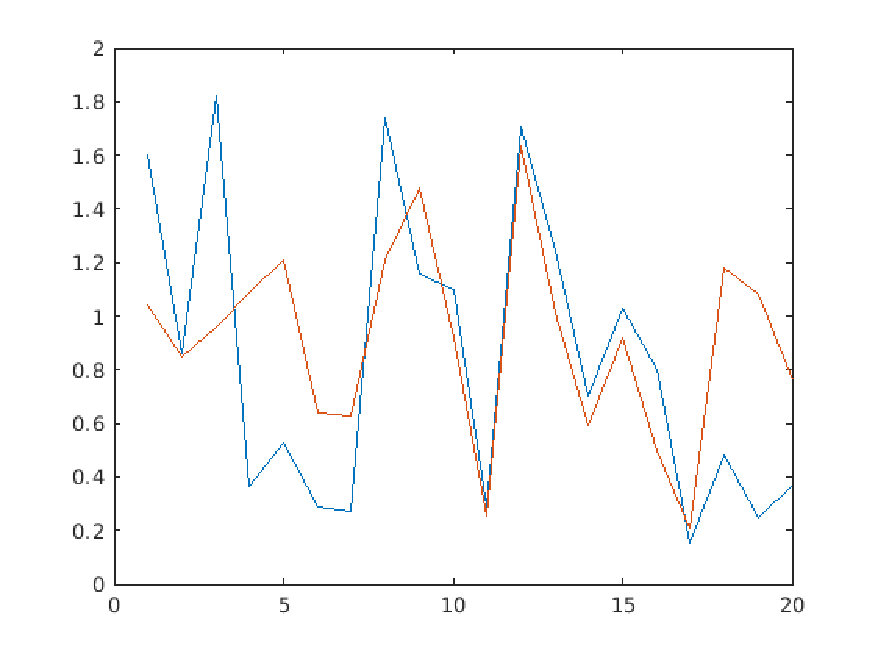
\includegraphics[width=0.5\textwidth]{simres.pdf}
 \end{center}
 \caption{Ergebnisfenster zur Daten-Visualisierung mittels plot-Befehl.}\label{abb:solman_matlab_simres}
\end{figure}

In \matlab{} existiert eine Vielzahl von Diagrammtypen und Visualisierungsm�glichkeiten, die per Kommandozeile oder graphischem Bedienerinterface (siehe Men�leiste \glqq PLOTS\grqq) angesprochen werden k�nnen.
Einige der weiterf�hrenden Plotbefehle sind unten noch einmal zusammenfassend aufgef�hrt. In den Texten und �bungen des Buches sind \mscre angegeben, die von den meisten dieser Befehle Gebrauch machen. 
\begin{table}%
\caption{Befehle f�r graphische Ausgabe.}
\smallskip
\begin{tabular}{|L{1.3cm}L{2.7cm}|L{1.3cm}L{2.7cm}|L{1.3cm}L{2.7cm}|}
\hline\noalign{\smallskip}
Funktion& Beschreibung &Funktion& Beschreibung &Funktion& Beschreibung \\
\noalign{\smallskip}\svhline\noalign{\smallskip}
\rule{0pt}{6pt} plot & 2-dimensionales Diagramm & semilogx & Diagramm mit logarithmischer x-Achse &  & schattierte Fl�che 3-dimensional\\
\hline\noalign{\smallskip}
\rule{0pt}{6pt} subplot  & Matrixanordnung von Diagrammen& semilogy & Diagramm mit logarithmischer y-Achse  & mesh & 3-dimensionales Gitterdiagramm\\
\hline\noalign{\smallskip}
\rule{0pt}{6pt} loglog  & Doppelt-logarithmisches Diagramm & surf & 3-dimensionale schattierte Oberfl�che& grid & Gitterlinien im Diagramm\\
\noalign{\smallskip}\hline\noalign{\smallskip}
\end{tabular} \label{tab:solman_matlab_plot}
\end{table}

Bitte beachten Sie die Skripte im Text f�r die verschiedenen Verwendungen dieser Befehle.

%-----------------------------------------------------------------------------------------------------------------------------------------------------------------------------
%\newpage
\section{Animationen} \label{kap:solman_matlab_film}
Mit \matlab{} kann man anschauliche Animationen erstellen. Nehmen wir als Beispiel eine sich ausbreitende ged�mpfte Welle. Man erstellt zun�chst ein Raum- und Zeitarray, gibt dann dieses Array bei jedem Zeitschritt graphisch aus und speichert den Plotframe in einem Array $M$ mit \textcolor{cyan}{\texttt{getframe}} ab. Man h�lt dann das Programm f�r eine kurze Zeit an (\zb \textcolor{cyan}{\texttt{pause}(0.1)} ). Den gesamten Ablauf kann man als Film mit 15 Bildern pro Sekunde als AVI-Datei abspeichern. Ein Beispiel ist hier angegeben:\\
\begin{lstlisting} [frame=single]
clear all
x=0:0.01:1;          % Raum-Array
t=0:0.01:1;          % Zeit-Array
nt=length(t);        % Zeitschritte
figure();
for j=1:nt 
    y=exp(-t(j)).*sin(2*pi*(x-t(j)));  % Wanderwelle
    plot(x,y,'color','r','linewidth',2); % Plot f�r jeden Zeitschritt
    ylim([-1 1]);
    grid on;
    M(j) = getframe; % speichere Movie Frames 
    pause(0.05);     % kurz pausieren
end 
movie(M, 1, 15)      % einmal mit 15 Bildern pro Sekunde abspielen
movie2avi(M,'wave'); % erstellt die Datei wave.avi 
\end{lstlisting} 
F�r die Ausgabe des Videos verwenden Sie folgenden Code:
\begin{lstlisting} [frame=single]
M = moviein(n); 
for j=l:n 
    plot 
    M(:,j) = getframe;
end 
movie(M) 
\end{lstlisting} 





%-----------------------------------------------------------------------------------------------------------------------------------------------------------------------------



\section{Skripte und benutzerdefinierte Funktionen} \label{kap:solman_matlab_files}
Ein \mscr, \zb mit \textcolor{blue}{test.m} bezeichnet, ist eine Textdatei, die \matlab-Befehle in einer geeigneten Reihenfolge enth�lt, damit sie vom Programm interpretiert und ausgef�hrt werden kann. Kommentarzeilen beginnen mit dem Prozent-Zeichen $\%$. Eine einfache m-Datei kann aus dem Befehlsfenster erstellt werden, indem der Befehl \textcolor{cyan}{$>>$ \texttt{ diary test.m }} gefolgt von mehreren Befehlen eingegeben wird, die eingeschlossen oder getestet werden sollen. Die Datei kann dann durch Eingabe von \textcolor{cyan}{$>>$ texttt{diary off }} geschlossen und �ber den \matlab-Editor oder einen anderen Texteditor aufgerufen werden. Durch Aufrufen des Namens der Datei im \matlab-Befehlsfenster; \dh durch Eingabe von \textcolor{cyan}{$>>$ \texttt{test} } wird die \matlab-Engine damit fortfahren, es zu interpretieren und die erforderliche Ausgabe zu erzeugen. Alle Fehler im Skript werden im Befehlsfenster angezeigt und k�nnen mit dem Texteditor behoben werden. 
\matlab{} hat viele eingebaute Funktionen, wie vom n�chsten Abschnitt beschrieben werden soll. Ein Benutzer kann auch eigene Funktionen erstellen. Eine Benutzerfunktion in \matlab{} ist entweder auch eine \textcolor{blue}{FunktionsName.m}-Datei oder aber sie wird am Ende des \matlab{} Files angegeben. Als Beispiel wolle wir die numerische Ableitung von $\sin\lk x\rk$ bei $x$ berechnen. Wir erstellen eine Skriptdatei mit dem Namen \textcolor{blue}{SinusAbleitung.m}: 
\begin{lstlisting} [frame=single]
function [F] = SinusAbleitung(x,del)
% Ableitung von sin(x) bei x im Intervall [x,x+del]
F = (sin(x+del)-sin(x))/del; 
\end{lstlisting} 
Sobald die Textdatei mit den obigen Zeilen unter dem Namen \textcolor{blue}{SinusAbleitung.m} gespeichert ist, kann sie �ber eine Zeile in einem \mscr aufgerufen werden. Zur Berechnung der Ableitung von $\sin\lk x\rk$ bei $x=\pi/3$ ben�tigen. Ist die Datei im Arbeitsverzeichnis gespeichert, so erh�lt man \zb:
\begin{lstlisting} [frame=single]
>>SinusAbleitung(pi/3,l.e-3) 
ans=0.5000
\end{lstlisting} 
Die Eingabe des Hilfeaufrufs im Befehlsfenster ergibt die Ausgabe:
\begin{lstlisting} [frame=single]
>>help SinusAbleitung
Ableitung von sin(x) bei x im Intervall [x,x+del]
\end{lstlisting} 
Dies ist die Zeile, die im Skript selbst als Kommentar eingef�gt wurde. Es ist wichtig, Kommentare innerhalb der Funktionen zu schreiben, um sich an ihre Verwendung zu erinnern und zu dokumentieren, dass solche Funktionen (im Arbeitsverzeichnis) vorhanden sind. 
%-----------------------------------------------------------------------------------------------
\section{Einige mathematische Funktionen}  \label{kap:solman_matlab_func}

Tabelle \ref{tab:solman_matlab_func} f�hrt einige h�ufig verwendete, vordefinierte \matlab-Funktionen auf.
\begin{table}%
\caption{Auswahl vordefinierter mathematischer Funktionen.}
\smallskip
\begin{tabular}{|L{1.3cm}L{2.7cm}|L{1.3cm}L{2.7cm}|L{1.3cm}L{3.5cm}|}
\hline\noalign{\smallskip}
Funktion& Beschreibung &Funktion& Beschreibung &Funktion& Beschreibung \\
\noalign{\smallskip}\svhline\noalign{\smallskip}
\rule{0pt}{6pt} $\tan$   & Tangens & $\min$ & kleinstes & $\tril$ &unterer dreieckiger Teil der Matrix \\
\hline\noalign{\smallskip}
\rule{0pt}{6pt} $\arcsin$   & Arcus Sinus & $\sign$ & signum & $\size$ & Gr��e einer Matrix\\
\hline\noalign{\smallskip}
\rule{0pt}{6pt} $\acos$   & Arcus Cosinus & $\length$ & L�nge eines Vektors& $\dett$ & Determinante  \\
\hline\noalign{\smallskip}
\rule{0pt}{6pt} $\arctan$   & Arcus Tangens & $\sort$ & aufsteigend sortierte Reihenfolge& $\inv$ & Inverse einer Matrix\\
\hline\noalign{\smallskip}
\rule{0pt}{6pt} $\exp$   & Exponentialfunktion & $\summ$ & Summe der Elemente einer Matrix & $\rand$ & mit Zufallszahlen gef�llte Matrix\\
\hline\noalign{\smallskip}
\rule{0pt}{6pt} $\log$   & nat�rlicher Logarithmus & $\prodd$ & Produkt der Elemente einer Matrix& $\rref$ & reduziert die Zeilenstufen einer Matrix\\
\hline\noalign{\smallskip}
\rule{0pt}{6pt} $\sin$   & Sinus & $\ceil$ & gegen positiv unendlich runden& $\diag$ & Diagonale einer Matrix extrahieren oder diagonale Matrix bilden\\
\hline\noalign{\smallskip}
\rule{0pt}{6pt} $\cos$   & Kosinus & $\max$ & gr��te Komponente & \odezd{}, \linebreak \odevf{} & L�sungsalgorithmus f�r Differentialgleichungen (Kap. \ref{kap:solman_matlab_dgl}) \\
\hline\noalign{\smallskip}
\rule{0pt}{6pt} abs   & absoluter Wert & median & Medianwert & $\eig$ & Eigenwerte und Eigenvektoren\\
\hline\noalign{\smallskip}
\rule{0pt}{6pt} $\sqrtt$   & Quadratwurzel & $\mean$ & Mittelwert & $\poly$ &Polynom\\
\hline\noalign{\smallskip}
\rule{0pt}{6pt} $\rem$   & Rest& $\std$ & Standardabweichung & $\quaddd$ & numerische Integration\\
\hline\noalign{\smallskip}
\rule{0pt}{6pt} $\round$   & auf n�chsten Integer Wert aufrunden& $\eye$ & Identit�tsmatrix & $\fzero $ & Nullstellen einer Funktion\\
\hline\noalign{\smallskip}
\rule{0pt}{6pt} $\floor$   & auf n�chsten Integer Wert abrunden& $\zeros$ & Matrix aus Nullen & $\roots$ & Wurzeln von Polynomen\\
\hline\noalign{\smallskip}
\rule{0pt}{6pt} $\modd$   & Modulo & $\ones$ & Matrix aus Einsen  & besselj & Bessel-Funktion erster Art\\
\noalign{\smallskip}\hline\noalign{\smallskip}
\end{tabular} \label{tab:solman_matlab_func}
\end{table}

Eine vollst�ndige Beschreibung der Funktionen findet man �ber die Eingabe des Hilfebefehls \mlcmd{help <Befehl>}.

%-----------------------------------------------------------------------------------------------
\newpage
\section{Programmierung} \label{kap:solman_matlab_prog}
Unter Programmierung in \matlab{} wollen wir eine Abfolge von Befehlen in einem \mscr verstehen, um wiederholte Berechnungen durchzuf�hren und Berechnungen allgemein verf�gbar zu machen. Programmieren ist \zb wichtig, wenn Schleifen und logische Anweisungen in Verbindung mit eingebauten oder benutzerdefinierten Funktionen verwendet werden. Wir geben einige Beispiele daf�r an:
\begin{lstlisting} [frame=single]
for i=l:1:1000
    x(i)=i*2;
    y(i)=sqrt(x(i));
end
\end{lstlisting} 
Die Zeilen erstellen ein 1000-Elemente-Array f�r $x$ zwischen $2$ und $2000$, f�r das die Quadratwurzel berechnet und im Array f�r $y$ gespeichert wird. In \matlab{} gibt es viel einfachere M�glichkeiten, dasselbe zu tun, das Beispiel demonstriert nur die Verwendung von Schleifen. Ein Beispiel f�r eine andere Programmierung mit dem gleichen Ergebnis:
\begin{lstlisting} [frame=single]
x = 2:2:2000;
y = sqrt(x);
\end{lstlisting} 
Ein Beispiel f�r eine if-else-Anweisung ist im Folgenden zu sehen, in dem in der Matrix $y$  alle ganzzahligen Quadratzahlen von 1 bis 1000 und in $z$ alle anderen einsortiert werden:
\begin{lstlisting} [frame=single]
ky=1;
kz=1;
for i=1:1000
    x(i)=sqrt(i);
    if abs(round(x(i))-x(i)) == 0
       y(ky) = i;
       ky = ky+1;
    else
       z(kz) = i;
       kz = kz+1;
    end
end
\end{lstlisting} 

%-----------------------------------------------------------------------------------------------
%\newpage
\section{Nullstellen von Funktionen} \label{kap:solman_matlab_roots}

Die eingebaute \matlab-Funktion \mlcmd{fzero} ist sehr n�tzlich und kann verwendet werden, um die Nullstellen einer Funktion zu bestimmen. Wir suchen \zb den Wert von $x$, bei dem die Beziehung $x = \e^{-x^2}$ erf�llt ist. 
\begin{lstlisting} [frame=single]
>>fzero('x-exp(-x^2)',0.5)
ans=0.6529
\end{lstlisting} 
wobei wir 0.5 als initialen Sch�tzwert verwendet haben. Eine vollst�ndige Beschreibung der Funktion \mlcmd{fzero} wie f�r alle anderen Funktionen finden man �ber den Hilfebefehl. Nat�rlich k�nnen wir auch die Nullstellen von benutzerdefinierte Funktionen bestimmen.\\
Ein weiteres Beispiel ist Berechnung von Wurzeln von Polynomen. Dazu kann die eingebaute Funktion \mlcmd{roots} verwendet werden. Als Beispiel berechnen wird die Nullstellen (Wurzeln) des  Polynoms 5. Ordnung $x^5+6x^3-2x+5$:
\begin{lstlisting} [frame=single]
>>x = roots([ 1 0 6 0 -2 5])
x =
  -0.0590 + 2.5180i
  -0.0590 - 2.5180i
  -1.0000 + 0.0000i
   0.5590 + 0.6897i
   0.5590 - 0.6897i
\end{lstlisting} 
Die L�sung besteht aus einer reellen und vier jeweils konjugiert komplexen Wurzeln. In Umkehrung gilt unter Verwendung des \mlcmd{poly}-Kommandos:
\begin{lstlisting} [frame=single]
>> poly(x)

ans =
    1.0000   -0.0000    6.0000   -0.0000   -2.0000    5.0000
\end{lstlisting} 

%-----------------------------------------------------------------------------------------------------------------------------------------------------------------------------
\section{Numerische Integration} \label{kap:solman_matlab_int}
Numerische Integration ist mit \matlab{} sehr einfach. Eine M�glichkeit besteht in der Nutzung der integrierten \mlcmd{quad} Funktion. Ein Beispiel daf�r ist die Integration der $\sin^2(x)$-Funktion �ber das Intervall $\lek 0, 2\pi\rek$ :
\begin{lstlisting} [frame=single]
>>quad('sin(x).^2',0, 2*pi);
ans =3.1416
\end{lstlisting} 
Hier haben wir eine vom Benutzer eingebauten Funktion inline benutzt. Man beachte die Operatoren f�r die elementweise Ausf�hrung (\zb .*). Alternativ kann man die zu integrierende Funktion �ber eine \textit{inline} Anweisung oder ein Handle @ auf eine zuvor definierte Funktion erzeugen.
\begin{lstlisting} [frame=single]
>> g=inline('2*x.^3+x.^5.*sin(x).^2');
>> quad(g,0,pi)
ans=86.4451 
\end{lstlisting} 
Hier wurde die Funktion $2 x^3+x^5 \sin^2(x) $ auf $\lek 0, \pi\rek$ integriert. Mit Handle sieht das entsprechende \mscr folgenderma�en aus:
\begin{lstlisting} [frame=single]
int3 = quad(@myfunc,0,pi);
function gh = myfunc(x)
    gh = 2*x.^3+x.^5.*sin(x).^2;
end
int3=86.4451 
\end{lstlisting} 


%-----------------------------------------------------------------------------------------------------------------------------------------------------------------------------
%\newpage
\section{Differentialgleichungen} \label{kap:solman_matlab_dgl}

Eine wesentliche F�higkeit von \matlab{} ist die numerische L�sung von Differentialgleichungen\index{Differentialgleichung} (DGL). Bei der numerischen L�sung von DGL bestimmt man ausgehend von Anfangsbedingungen\index{Anfangsbedingungen} (AB) eine Folge von Wertepaaren $(t_0, y_0)$, $(t_1, y_1)$, $(t_2, y_2), \ldots $, die den Verlauf der gesuchten Funktion $y(t)$ ann�hern sollen. In \matlab{} wird unterschieden zwischen gew�hnlichen Differentialgleichungen\index{Differentialgleichung!gew�hnliche} (ODE, \textit{Ordinary Differential Equations}), differential-algebraischen
Gleichungen \index{Differential-Algebraisches System} (DAE, \textit{Differential Algebraic Equations}) \ua Die in \matlab{} enthaltenen numerischen L�sungsalgorithmen (\textit{Solvers})\index{Solver} k�nnen f�r eine
Vielzahl von Systemen eingesetzt werden, die durch Differentialgleichungen beschreibbar sind. Ausf�hrliche Behandlung zu Differentialgleichungen und deren numerischer L�sung finden sich in \cite{Riley2006, Felder2016, Fischer2014}.

\subsection{Gew�hnliche Differentialgleichungen (ODE)} \label{kap:solman_matlab_ODE}
 
Mathematisch l�sst sich eine gew�hnliche Differentialgleichung mit dem Zustandsvektor $\vec{Y}$
und dem Zeitargument $t$, einer beliebigen vektorwertigen Funktion $\vec{f}$ und dem Anfangsbedingungen $\vec{Y}_0$
zum Zeitpunkt $t_0$ als Differentialgleichungssystem erster Ordnung darstellen:
	\begin{align}
\frac{\D \vec{Y}}{\D t} = \vec{f}(t,\vec{Y}) ~~~~\text{mit} ~~~~\vec{Y}(t_0) = \vec{Y}_0\,. \label{eq:solman_matlabdgl01}
	\end{align}
\matlab{} hat die F�higkeit, solche Differentialgleichungen mit eingebauten Funktionen wie \textcolor{cyan}{\texttt{ode45}} oder \textcolor{cyan}{\texttt{ode23}} \ua zu l�sen. Wir wollen als Beispiel ein eindimensionales Problem l�sen. Als Beispiel haben wir die DGL $\dot{y}=(y-t^2)\e^{-t}$ f�r $y\lk t\rk$ auf dem Intervall $\lek 0,20\rek$ mit der Anfangsbedingung $t=0, y=1$ ausgew�hlt. In \matlab{} kann dies wie folgt erreicht werden: 
\begin{lstlisting} [frame=single]
tspan=linspace(0,10);
[t,y]=ode45(@myfunc,tspan,1 ); 
figure()
plot(t,y)
function f = myfunc(t,y)
  f=(y-t.^2).*exp((-t));
end
\end{lstlisting} 
Zur L�sung von Differentialgleichungen gem�� \eqref{eq:solman_matlabdgl01} stehen in \matlab{} verschiedene Algorithmen (Solver) zur Verf�gung. Die \matlab-Solver unterscheiden sich hinsichtlich ihres Verhaltens bei sogenannten steifen Differentialgleichungen.\index{Differentialgleichung!steife} Eine Differentialgleichung wird als steif (\textit{stiff}) bezeichnet, wenn die Verfahren wegen ihres beschr�nkten Stabilit�tsgebietes erhebliche Genauigkeitsprobleme haben oder wenn Schaltvorg�nge zu ber�cksichtigen sind. Diese treten bis auf wenige Ausnahmen in den im Buch betrachteten F�llen nicht auf. Bei der Wahl der Integrationsverfahren hat sich deshalb folgendes Vorgehen bew�hrt. Zuerst
w�hlt man den Solver \textcolor{cyan}{\texttt{ode45}}, welcher eine Implementierung eines expliziten Runge-Kutta-Verfahrens\index{Runge-Kutta-Verfahren} 5. Ordnung ist (siehe die \onlineZ \bzw \cite{Riley2006, Fischer2014, Natt2020}). Dann �berpr�ft man die Ergebnisse auf Stabilit�t und kann gegebenenfalls einen Solver wie \textcolor{cyan}{\texttt{ode15s}} oder \textcolor{cyan}{\texttt{ode23s}} zur Berechnung probieren. Wir empfehlen, sich die Skripte des Buches f�r die einzelnen Beispiele anzuschauen oder die Befehle \textcolor{cyan}{\texttt{ help ode45}} \bzw \textcolor{cyan}{\texttt{ode15s}} in das Befehlsfenster einzugeben, um weitere Informationen und Details zu erhalten. 

Bisher haben wir nur DGL \bzw DGL-Systeme mit ersten Ableitungen betrachtet. In der Physik und insbesondere in der Mechanik treten aber vorwiegend DGL-Systeme zweiter Ordnung nach der Zeit auf, \dh wir haben eigentlich System der Form:
	\begin{align}
\frac{\D^2 \vec{\tilde{Y}}}{\D t^2} = \vec{f}(t,\vec{\tilde{Y}}) ~~~~\text{mit} \vec{}(t_0) = \vec{\tilde{Y}}_0\,. \label{eq:solman_matlabdgl02}
	\end{align}
Diese kann man aber problemlos in ein System 1. Ordnung gem�� \eqref{eq:solman_matlabdgl01} �berf�hren. Wir wollen das f�r ein DGL-System f�r 3 Koordinaten $(\tilde{Y}_1, \tilde{Y}_2, \tilde{Y}_3)$ zeugen.
Wir schreiben dazu:
\begin{align}
	Y_1 &= \tilde{Y}_1,~~~~ &Y_2 = \D \tilde{Y}_1 / \D t \nonumber \\
	Y_3 &= \tilde{Y}_2,~~~~ &Y_4 = \D \tilde{Y}_4 / \D t  \label{eq:solman_matlabdgl03} \\
	Y_5 &= \tilde{Y}_3,~~~~ &Y_6 = \D \tilde{Y}_6 / \D t \nonumber \,.
\end{align}
Das �quivalente $2n$-dimensionale DGL-System 1. Ordnung zum $n$-dimensionalen System 2.Ordnung \eqref{eq:solman_matlabdgl02} lautet dann.
\begin{align}
	\dot{Y}_1 &= Y_4 = f_1(Y_4)~ , ~~&\dot{Y}_4 = f_4(t, \vec{Y}) \nonumber \\
	\dot{Y}_2 &= Y_5 = f_2(Y_5)~ , ~~&\dot{Y}_5 = f_5(t, \vec{Y})  \label{eq:solman_matlabdgl04} \\ 
	\dot{Y}_3 &= Y_6 = f_3(Y_6)~ , ~~&\dot{Y}_6 = f_6(t, \vec{Y}) \nonumber \,.
\end{align}
Dieses Verfahren haben wir \zb bei der Berechnung der Wirkungen der Corioliskraft im Kapitel Physik der Bewegung angewendet. Dort wurde die die Funktion $\vec{f}$ mit Parametern versehen und als \textcolor{cyan}{\texttt{CoriolisDGLS(t,Y,Omeg,Cphi,Sphi,G,Eta)}} definiert:
\begin{lstlisting} [frame=single]
% Differentialgleichungssystem f�r Corioliskraft
function dY = CoriolisDGLS(t,Y,Omeg,Cphi,Sphi,G,Eta)
  dY    = zeros(6,1);
  dY(1) = Y(4); dY(2) = Y(5); dY(3) = Y(6);
  vbet  = sqrt(Y(4)^2+Y(5)^2+Y(6)^2);
  dY(4) = 2*Omeg*Sphi*Y(5)-Eta*vbet*Y(4);
  dY(5) = -2*Omeg*Sphi*Y(4)-2*Omeg*Cphi*Y(6)-Eta*vbet*Y(5);
  dY(6) = 2*Omeg*Cphi*Y(5)-G-Eta*vbet*Y(6);  
end
\end{lstlisting} 
Wir hatten bisher auch implizit angenommen, dass das DGL-System in expliziter Form, \dh in der Form $\D \vec{Y}/\D t = \vec{f}(t,\vec{Y})$ vorliegt. H�ufig aber findet man es eher in der Form:
\begin{equation} 
    \mathbb{M}(t,\vec{Y}) \dot{\vec{Y}} = f(t,\vec{Y})\,, \label{eq:solman_matlabdgl05}
\end{equation} 
worin $\mathbb{M}$ die sogenannte Massen-Matrix ist. %Wir finden eine solche Form \ua in der \probref {bew_Hantelwurf}:
\begin{align*}
    \begin{bmatrix}
          1 & 0  & 0 & 0 & 0 & 0 \\
          0 & m_1+m_2  & 0 & 0 & 0 & -m_2\,L\sin Y_5 \\
          0 & 0  & 1 & 0 & 0 & 0 \\
          0 & 0  & 0 & m_1+m_2 & 0 & m_2\,L\cos Y_5\\
          0 & 0  & 0 & 0 & 1 & 0 \\
          0 & -L\sin Y_5  & 0 & L \cos Y_5 & 0 & L^2 \\
    \end{bmatrix}
    \begin{bmatrix}
          \dot{Y}_1 \\
          \dot{Y}_2 \\
          \dot{Y}_3 \\
          \dot{Y}_4 \\
          \dot{Y}_5 \\
          \dot{Y}_6 \\
    \end{bmatrix}
    =
    \begin{bmatrix}
          Y_2 \\
          m_2\,L\,{Y_6}^2 \cos Y_5 \\
          Y_4 \\
          m_2\,L\,{Y_6}^2 \sin Y_5 - (m_1+m_2)\,g\\
          Y_6 \\
          -g\,L\cos Y_5\\
    \end{bmatrix}
\end{align*} 
Das System kann also in der Form einer Matrixgleichung gem�� \eqref{eq:solman_matlabdgl05} geschrieben werden. Die weitere Berechnung der L�sung diese DGL-Systems mittels \matlab{} mit dem \texttt{ode45} Solver ist v�llig analog mit der beschriebenen Vorgehensweise zur L�sung von Gleichungssystemen der Form \eqref{eq:solman_matlabdgl04}. Lediglich muss hier beim Setzen der Optionen f�r den \texttt{ode45} Solver mittels \textcolor{cyan}{\texttt{odeset}} die Massenfunktion \textcolor{cyan}{\texttt{'Mass'}}  ($M = \text{Mass}(t,Y,P)$) aufgerufen werden. Dabei wird mit $P$ auch eine Struktur mit dem Parametersatz �bergeben.%in unserem Fall $(m_1, m_2, L, g)$.
\begin{lstlisting} [frame=single]
opts = odeset('Mass',@(t,Y) Mass(t,Y,P1));
[t,Y1] = ode45(@(t,Y) f(t,Y,P1),tspan,Y01,opts);
function M = Mass(t,q,P)
% Extrahiere Parameter
m1 = P.m1; m2 = P.m2; L = P.L; g = P.g;
% Massen-Matrix
M = zeros(6,6);
M(1,1) = 1;
M(2,2) = m1 + m2;
M(2,6) = -m2*L*sin(q(5));
M(3,3) = 1;
M(4,4) = m1 + m2;
M(4,6) = m2*L*cos(q(5));
M(5,5) = 1;
M(6,2) = -L*sin(q(5));
M(6,4) = L*cos(q(5));
M(6,6) = L^2;
end
% DGL Funktion f
function dYdt = f(t,Y,P) 
% Extrahiere Parameter
m1 = P.m1; m2 = P.m2; L = P.L; g = P.g;
% DGL
dYdt = [Y(2)
        m2*L*Y(6)^2*cos(Y(5))
        Y(4)
        m2*L*Y(6)^2*sin(Y(5))-(m1+m2)*g
        Y(6)
        -g*L*cos(Y(5))];
end
\end{lstlisting} 

\textbf{\textit{Setzen der Optionen f�r Solver:}} \\
Unter Ber�cksichtigung von Optionseinstellungen f�r den Solver und Parameter�bergaben an die Funktionen \textcolor{cyan}{\texttt{dYdt}} lauten die allgemeinen Aufrufe der
verschiedenen Solver:
\begin{lstlisting} [frame=single]
options = odeset(�name1�,wert1,�name2�,wert2,...);
[t,Y] = solver(@dYdt,tspan,Y0,options,p1,p2,...);
\end{lstlisting} 
Die Parameter p1, p2, ... werden an die Funktion dYdt und an alle evtl. in den Optionen
definierten Funktionen als zus�tzliche Argumente �bergeben. Eine Struktur \textcolor{cyan}{\texttt{options}} mit Standardvorbelegungen
wird durch das Kommando \textcolor{cyan}{\texttt{odeset}} erzeugt, damit wird das Verhalten der Solver gesteuert. Folgende Werte k�nnen gesetzt werden.

\begin{table}%
\caption{Auswahl von Werten (Standardwerten) f�r das Setzen von Optionen mit \textcolor{cyan}{\texttt{odeset}}.}
\smallskip
\begin{tabular}{|L{4cm}|L{6cm}|}
\hline\noalign{\smallskip}
Optionsparameter  & Wert  \\
\noalign{\smallskip}\svhline\noalign{\smallskip}
\rule{0pt}{6pt} AbsTol &[ positive scalar or vector \textcolor{red}{(1e-6)} ] \\
\hline\noalign{\smallskip}
\rule{0pt}{6pt} RelTol &[ positive scalar \textcolor{red}{(1e-3)} ]\\
\hline\noalign{\smallskip}
\rule{0pt}{6pt} Mass &[ matrix | function\_handle ]\\
\hline\noalign{\smallskip}
\rule{0pt}{6pt} Events &[ function\_handle ] \\
\hline\noalign{\smallskip}
\rule{0pt}{6pt} MassSingular &[ yes | no | \textcolor{red}{(maybe)} ]\\
\hline\noalign{\smallskip}
\rule{0pt}{6pt} Events &[ function\_handle ] \\
\hline\noalign{\smallskip}
\rule{0pt}{6pt} Jacobian &[ matrix | function\_handle]\\
\hline\noalign{\smallskip}
\rule{0pt}{6pt} NormControl &[ on | \textcolor{red}{(off)} ]\\
\hline\noalign{\smallskip}
\rule{0pt}{6pt} Events &[ function\_handle ] \\
\hline\noalign{\smallskip}
\rule{0pt}{6pt} NonNegative &[ vector of integers ]\\
\hline\noalign{\smallskip}
\rule{0pt}{6pt} Events &[ function\_handle ] \\
\hline\noalign{\smallskip}
\rule{0pt}{6pt} InitialStep &[ positive scalar ]\\
\hline\noalign{\smallskip}
\rule{0pt}{6pt} MaxStep &[ positive scalar ]\\
\hline\noalign{\smallskip}
\rule{0pt}{6pt} OutputFcn &[ function\_handle ]\\
\hline\noalign{\smallskip}
\rule{0pt}{6pt} OutputSel &[ vector of integers ] \\
\hline\noalign{\smallskip}
\rule{0pt}{6pt} InitialSlope &[ vector ] \\
\noalign{\smallskip}\hline\noalign{\smallskip}
\end{tabular} \label{tab:solman_matlab_odeset}
\end{table}
In eckigen Klammern werden die m�glichen Werte \bzw rot in runden Klammern die
Standardwerte angezeigt. Die genauere Bedeutung der einzelnen Parameter der Options-Struktur wird in den einzelnen \mscren erl�utert und auch ersichtlich. Im Allgemeinen braucht man nur wenige Optionen zu ver�ndern und kann vielfach mit Standardwerten arbeiten. F�r weitere Details verweisen wir auf das Hilfemen� von \matlab{}. \\

\textbf{\textit{Event}-Behandlung:} \\
In vielen technischen Systemen spielen Schaltvorg�nge oder Unstetigkeiten
eine wichtige Rolle. Typische Beispiele sind Haftreibungsvorg�nge, Sto�vorg�nge oder 
das Verschwinden von Zwangskr�ften (siehe Kap. Physik der Bewegung).
Die numerischen Integrationsverfahren d�rfen �ber solche
Unstetigkeitsstellen nicht einfach hinwegintegrieren. Die Solver in \matlab{}
sind zu diesem Zweck mit Mechanismen zur Detektion solcher Unstetigkeiten, so
genannter \textit{Events}, ausgestattet. Die Solver sind in der Lage, w�hrend der Integration
die Schrittweite so anzupassen, dass die Nullstellen einer Event-Funktion exakt mit einem Integrationsschritt
getroffen werden. Wenn die Nullstelle erreicht wird, kann die Integration
entweder ganz normal fortgesetzt oder angehalten werden. Die Option \textcolor{cyan}{\texttt{events}} wird
benutzt, um die Funktion anzugeben, deren Nullstellen detektiert werden sollen. Die
Funktion muss die folgende Form besitzen:
\begin{lstlisting} [frame=single]
function [value,isterminal,direction] = ereignis(t,Y,p1,p2,...)
\end{lstlisting} 
Die Funktion \textit{Event} wird mit dem aktuellen Zeitpunkt t, dem Zustandsvektor Y und
evtl. weiteren Parametern p1, p2, ... aufgerufen. Die R�ckgabewerte haben die folgende
Bedeutung:
\begin{itemize}
	\item \textcolor{cyan}{\texttt{value}} ist ein Vektor, dessen Nulldurchg�nge vom Solver �berwacht werden. Das Element \textcolor{cyan}{\texttt{value(i)}} wird als i-tes Ereignis bezeichnet.
	\item \textcolor{cyan}{\texttt{isterminal(i)=1}} bedeutet, dass bei einem Nulldurchgang von \textcolor{cyan}{\texttt{value(i)}}= die numerische
Integration zu beenden ist. Wenn \textcolor{cyan}{\texttt{isterminal(i)=0}} ist, wird die Integration fortgesetzt.
	\item \textcolor{cyan}{\texttt{direction(i)=0}} hei�t, dass alle Nulldurchg�nge von \textcolor{cyan}{\texttt{value(i)}} zu detektieren
sind; bei \textcolor{cyan}{\texttt{direction(i)=1}} werden nur Nulldurchg�nge negativ zu positiv bzw.
bei \textcolor{cyan}{\texttt{direction(i)=-1}} nur Nulldurchg�nge von positiv zu negativ detektiert.
\end{itemize}
Die �berwachung von Ereignissen wird durch die Option \textcolor{cyan}{\texttt{events}} aktiviert:
\begin{lstlisting} [frame=single]
options = odeset(�Events�, @ereignis);
\end{lstlisting} 
Durch die Verwendung der Option \textcolor{cyan}{\texttt{events}} gibt der Solver weitere R�ckgabewerte aus:
\begin{lstlisting} [frame=single]
[t,Y,TE,YE,IE] = solver(@dYdt,tspan,Y0,options,p1,p2,...);
\end{lstlisting} 
Im Spaltenvektor TE werden die Zeitpunkte des Auftretens eines Events aus der Funktion
\textcolor{cyan}{\texttt{Ereignis}} zur�ckgegeben. Die Zeilen von YE enthalten den L�sungsvektor zu diesen
Event-Zeitpunkten. Die Werte in IE geben den Index des Elements \textcolor{cyan}{\texttt{value(IE)}} der
Ereignisfunktion an, bei der ein Nulldurchgang stattfand.\\

\textbf{Feste Ausgabeschrittweite der Solver:} \\
Der Solver \textcolor{cyan}{\texttt{ode45}} arbeitet mit einem verbesserten Runge-Kutta-Verfahren, mit dem die Schrittweite gesteuert werden.
Wegen dieser automatischen Schrittweitensteuerung legt textcolor{cyan}{\texttt{ODE45}} selbst fest, in wie viele Zeitschritte das vorgegebene Zeitintervall unterteilt wird. 
Die Zeitschritte sind im Allgemeinen nicht mehr �quidistant, deshalb ist die Matrix der Ergebnisse Y immer im Zusammenhang mit dem Ergebnisvektor
t zu sehen. Die L�nge des Ergebnisvektors kann gegebenenfalls mit der \matlab-Funktion \textcolor{cyan}{\texttt{length}} erfragt werden. H�ufig braucht man aber doch �quidistante Ausgabewerte. Hier gibt es zwei M�glichkeiten.\\
\begin{itemize}
	\item \textcolor{cyan}{\texttt{odeset}} ohne Eventfunktion:\\
                In diesem Fall kann man durch explizite Angabe der Range in �quidistanter Form eine �quidistante Ausgabe f�r Y erzwingen.
\begin{lstlisting} [frame=single]
Y0 = [100,0]
tspan = linspace(1,5,101)
opt=odeset('AbsTol',1.e-9,'RelTol',1.e-7);           
[t,Y]=ode45(@DGL,tspan,Y0,opt); 
plot(t,Y(:,1)); %t, hat �quidistante Elemente
function dY = DGL(t,Y)
g  = 9.81;  
dY = [Y(2); -g];
end
\end{lstlisting} 

	 \item \textcolor{cyan}{\texttt{odeset}} mit Eventfunktion:\\
                Das gerade beschriebene Verfahren funktioniert in diesem Fall wegen der Event bezogenen Schrittsteuerung nicht.
                Hier hilft nur, m�glichst viele Ausgabewerte zu berechnen und dann zu interpolieren.
                Wir haben dies \zb in \mlbewref{MurphysLaw.m} ausgef�hrt und geben hier das Listing an:
\begin{lstlisting} [frame=single]
options1=odeset('AbsTol',1.e-9,'RelTol',1.e-7,'events',@MyEvent1);
[t,Y,TE,YE,IE]=ode45(@dgl_Brett1,tspan,AB,options1,P1); 
% t,Y sind nicht �quidistant
% interpolieren, um �quidistante intervalle f�r den ode output zu erhalten
Yeq=interp1(t,Y,tspan); % Yeq ist nun �quidistanter
\end{lstlisting} 

\end{itemize}

\subsection{Differential-Algebraische Gleichungen (DAE)} \label{kap:solman_matlab_DAE}

H�ufig lassen sich DGLen der Mechanik durch eine Differentialgleichung
mit Masse-Matrix gem�� Gleichung \eqref{eq:solman_matlabdgl05} darstellen.
In der zeit- und zustandsabh�ngigen Masse-Matrix $\mathbb{M}$sind typischerweise Massen und
Tr�gheitsmomente des Systems enthalten. Wenn die Masse-Matrix nicht
singul�r\index{Matrix!nicht-singul�re} ist (siehe die \onlineZ), kann die Gleichung umgeformt werden und es existiert
eine L�sung f�r alle Anfangsbedingungen $t_0$ und $\vec{Y}_0$.
Bei nicht singul�rer Masse-Matrix sind alle Solver in der Lage, ein System gem�� Gleichung
\eqref{eq:solman_matlabdgl05} zu l�sen. 

Bei singul�rer Matrix\index{Matrix!singul�re} $\mathbb{M}(t,\vec{Y})$ stellt Gleichung \eqref{eq:solman_matlabdgl05}
eine differential-algebraische Gleichung (DAE)\index{Differential-Algebraisches System}  dar, die nur dann eine L�sung besitzt, wenn der Anfangswert
$\vec{Y}_0$ konsistent mit der DAE ist. Das bedeutet, es muss eine Anfangssteilheit
$\D \vec{Y}_0 / \D t$ existieren, so dass 
	\[\mathbb{M}(t,\vec{Y}_0) \D \vec{Y} / \D t |t_0 = f(t_0, )
	\]
ist. Bei nicht konsistenter Anfangsbedingung versucht der Solver in deren N�he eine konsistente zu finden
und das Problem mit diesen neuen Anfangswerten zu l�sen. DAEs k�nnen nur mit
den Solvern \textcolor{cyan}{\texttt{ode15s}} und \textcolor{cyan}{\texttt{ode23t}} behandelt werden. Der Solver \textcolor{cyan}{\texttt{ode23s}} kann nur
DAEs mit konstanter Masse-Matrix l�sen. In der Option \textcolor{cyan}{\texttt{Mass}} muss entweder eine
konstante Matrix oder ein Zeiger auf eine Funktion zur Ermittlung der Masse-Matrix
enthalten sein.\\
Ein nicht-getriebenes Pendel der L�nge L mit Reibung $F_\text{R}$ soll als Beispiel f�r eine Differentialgleichung
mit Masse-Matrix dienen und wird in die Form \eqref{eq:solman_matlabdgl05} gebracht. Zus�tzlich wird
angenommen, dass die Masse $m$ des Pendels mit der Zeit exponentiell abnimmt und
das Pendel nicht angetrieben wird. 
Als Differentialgleichungssystem mit Masse-Matrix ergibt sich:
\begin{align}
\dot{Y}_1 &= Y_2 ~~,~~m(t) \dot{Y}_1 = -m(t)\frac{g}{L}\sin{Y_1} - \frac{2\,F_\text{R}}{\pi L}\sin{Y_1} \arctan{10 Y_2} \, \label{eq:solman_matlabdgl07} \\
\rightarrow \mathbb{M}(t,\vec{Y}) &=  \begin{pmatrix}
        1 & 0 \\
        0 & m(t) 
        \end{pmatrix} \,.\label{eq:solman_matlabdgl08}
\end{align}
Die Funktion \textcolor{cyan}{\texttt{Ydot\_pendelmass}} repr�sentiert die rechten Seiten der Gleichungen in \eqref{eq:solman_matlabdgl07}.
\begin{lstlisting} [frame=single]
% DAE Pendel
% Daten, Anfangswerte, Zeitspanne, Optionen
L = 5; m0 = 30; g = 9.81; FR = 4; T = 15;
Y0 = [15/360*2*pi; 0];
tspan = [0 20]; 
%Damit der Solver die Masse-Matrix verwenden kann, muss sie ueber die Option Mass auf
%@mass gesetzt werden. Die Loesung erfolgt mit Solver ode15s 
options = odeset('Mass', @mass);
[t Y] = ode15s(@Ydot_pendelmass,tspan,Y0,options,L,m0,g,FR,T);
%-----------------------------------------------
% Ydot_pendelmass, DGL
function Ydot = Ydot_pendelmass(t,Y,L,m0,g,FR,T)
  m = m0*exp(-t/T);
  Ydot = [Y(2); -m*g/L*sin(Y(1)) - FR*2/pi*atan(10*Y(2))/L];
end
%-----------------------------------------------
% mass.m
% Berechnung der Masse-Matrix wird in der Funktion mass
% realisiert. Daten des Pendels als Parameter vom Solver uebergeben.
function M = mass(t,Y,L,m0,g,FR,T)
  M = [1 0; 0 m0*exp(-t/T)];
end
\end{lstlisting} 

\begin{lstlisting} [frame=single]
% Ausgabe
figure()
plot (t,Y(:,1));
hold on
plot (t,Y(:,2));
figure()
plot (t,m0*exp(-t/T));
\end{lstlisting} 
Als L�sung f�r $\varphi(t)=$Y(:,1) und $\dot{\varphi}(t)=$Y(:,2) �ber die Zeitspanne von 20 s ergibt sich der in \figref{solman_matlab_DAE}a dargestellte Verlauf.
In \figref{solman_matlab_DAE}b ist der zugeh�rige Masseverlauf dargestellt.
Eine etwas komplexere DAE haben wir im Kapitel Physik der Bewegung von K�rpern (Band I) mit dem \mscr \mlbewref{TrebSimDAE.m} behandelt:
\begin{lstlisting} [frame=single]
% Runge-Kutta-Verfahren-MATLAB ODE15s
opts = odeset('Mass',@(t,Y) Mass1(t,Y,P),'RelTol',1e-6);
[t,Y] = ode15s(@(t,Y) F1(t,Y,P),tv,AB1,opts);
% -------------------------------------------------------
% Massen-Matrix f�r Schleifphase (mit Zwangsbedingung)
function M = Mass1(t,q,P)
% Parameter extrahieren
JG  = P.JG; JW  = P.JW; JbW = P.JbW; JBG = P.JBG;
J0  = P.J0; b   = P.b; lW  = P.lW;
% Massen-Matrix aufstellen
M = zeros(7,7);
M(1,1) = 1; M(2,2) = J0; M(3,3) = 1; 
M(4,4) = JG; M(5,5) = 1; M(6,6) = JW; 
M(2,4) = +JBG*cos(q(1)-q(3)); M(4,2) = M(2,4);
M(2,6) = -JbW*cos(q(1)-q(5)); M(6,2) = M(2,6);
M(7,2) = -b*cos(q(1)); M(7,6) = lW*cos(q(5));
M(2,7) = M(7,2); M(6,7) = M(7,6);
end
% -------------------------------------------------------
% DGL Funktion
function dYdt = F1(t,Y,P)
% Parameter extrahieren
LG  = P.LG;  lW  = P.lW;  MG  = P.MG; mW  = P.mW; 
JBG = P.JBG; JbW = P.JbW; g   = P.g;   U0  = P.U0; b   = P.b; 
% DGL
dYdt = [Y(2);
 -JBG*Y(4)^2*sin(Y(1)-Y(3))+JbW*Y(6)^2*sin(Y(1)-Y(5))-U0*cos(Y(1));
 Y(4); 
 +JBG*Y(2)^2*sin(Y(1)-Y(3)) - MG*LG*g*cos(Y(3));
 Y(6);
 -JbW*Y(2)^2*sin(Y(1)-Y(5)) - mW*lW*g*cos(Y(5));
 -b*Y(2)^2*sin(Y(1)) + lW*Y(6)^2*sin(Y(5))];
end
\end{lstlisting} 

\begin{figure}[!htpb]
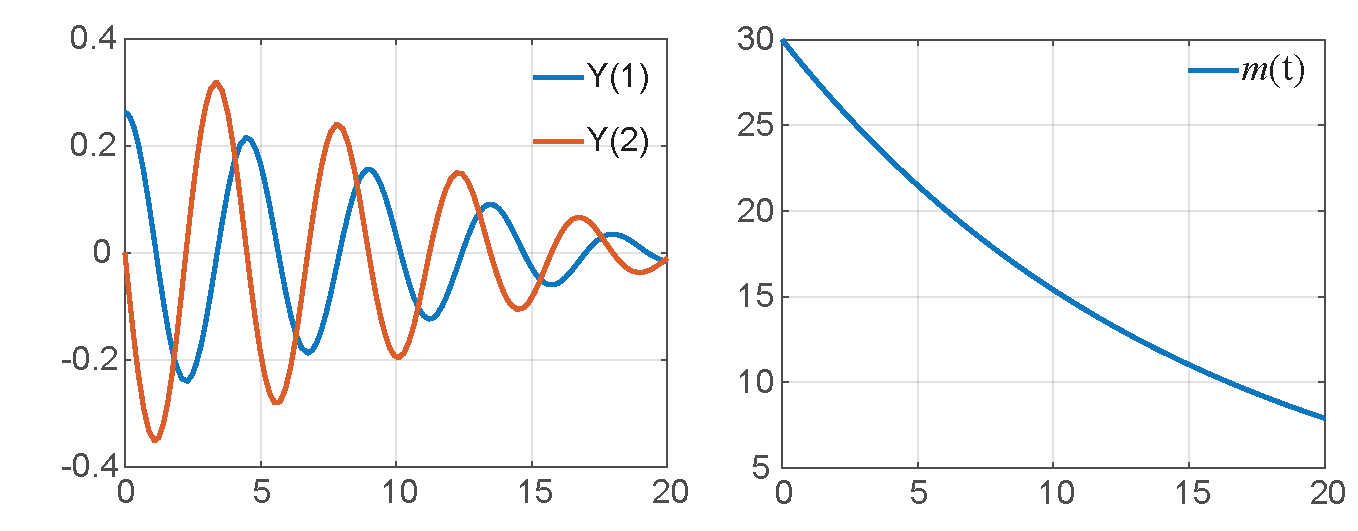
\includegraphics[width=\textwidth]{ExampleDAE.pdf}
\caption[Ergebnisfenster des \matlab-Programms f�r DAE-Berechnung.]{Ergebnisfenster des \matlab-Programms f�r DAE-Berechnung \eqref{eq:solman_matlabdgl07}.}\label{abb:solman_matlab_DAE}
\end{figure}

\subsection{Differentialgleichung mit Delay-Zeiten (DDE)} \label{kap:solman_matlab_DDE}

\newpage
\subsection{Partielle Differentialgleichungen (PDE)} \label{kap:solman_matlab_PDG}

In Anlehnung an die \matlab-Onlinehilfe unter
\url{https://de.mathworks.com/help/matlab/math/partial-differential-equations.html}
sei hier ein einfaches Beispiel der W�rmeleitungsgleichung 
\begin{align}
  \frac{\partial u}{\partial t} = 0.1\cdot\frac{\partial^2 u}{\partial x^2}
\end{align}
angegeben. Es handelt sich um eine parabolische Differentialgleichung, die die �rtliche und zeitliche �nderung der Temperatur $u(x,t)$ wiedergibt.
Dies mag ein eindimensional modellierter Stab sein, dessen Temperatur auf halben Niveau startet und dessen Enden hoher \bzw niedriger Temperatur ausgesetzt werden.
F�r die \matlab-Simulation sind die Angabe von (�rtlichen) Randbedingungen $u(0,t) = 0$ und $u(1,t) = 1$
\begin{lstlisting} [frame=single]
function [pl,ql,pr,qr] = WlgRandbedingungen(xl,ul,xr,ur,t)
  pl = ul;
  ql = 0;
  pr = ur - 1;
  qr = 0;
end
\end{lstlisting} 
sowie der (zeitlichen) Anfangsbedingung $u(x,0)=0.5$
\begin{lstlisting} [frame=single]
function u0 = WlgAnfangswerte(x)
  u0 = 0.5;
end
\end{lstlisting} 
erforderlich. Ebenso wie die Definition der PDE (mit diversen Anpassungsfaktoren $c,s$ f�r allgemeinere Problemklassen)
\begin{lstlisting} [frame=single]
function [c,f,s] = WlgPDE(x,t,u,dudx)
  c = 1;
  f = 0.1*dudx;
  s = 0;
end
\end{lstlisting} 
erfolgt dies in jeweils eigenen Funktions-Skripten. Der Aufruf des eigentlichen PDE-Solvers \mlcmd{pdepe} erfolgt mit
\begin{lstlisting} [frame=single]
% PDG Solver
x = linspace(0,1,200);
t = linspace(0,1,200);
u = pdepe(0,@WlgPDE,@WlgAnfangswerte,@WlgRandbedingungen,x,t)';
colormap hot
imagesc(t,x,u)
colorbar
xlabel('t')
ylabel('x')
\end{lstlisting} 
und liefert den �rtlichen und zeitlichen Temperaturverlauf f�r $0\le x\le 1$ und $0\le t \le 1$, siehe Abb. \ref{abb:solman_matlab_PDE}.
\begin{figure}[!htpb]
 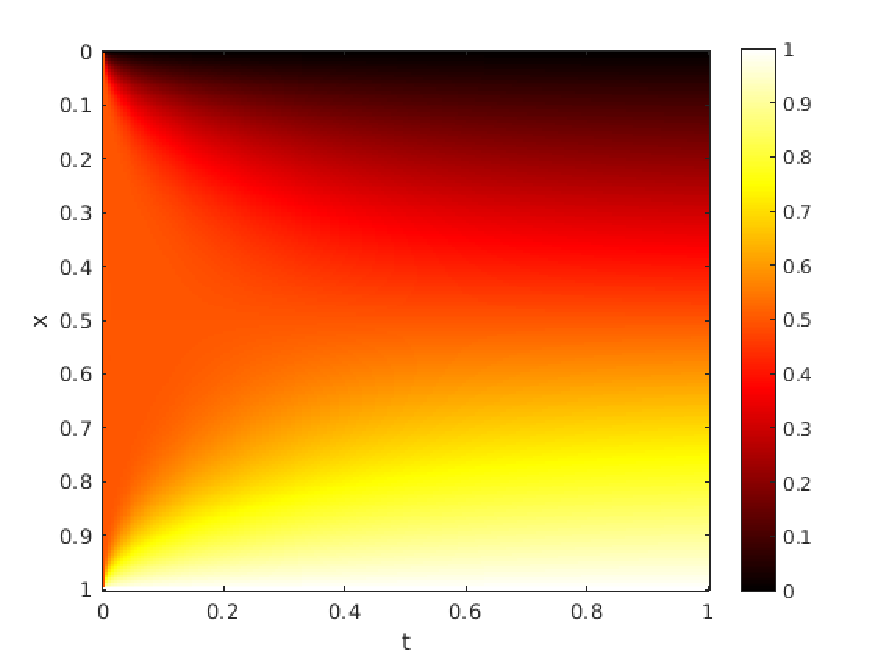
\includegraphics[width=\textwidth]{WlgPDGL.pdf}
 \caption[Ergebnisfenster des \matlab-Programms f�r PDE-Berechnung.]{Ergebnisfenster des \matlab-Programms f�r PDE-Berechnung.}
\end{figure}

%%%%%%%

\newpage
\section{Symbolische Berechnung}\label{kap:solman_matlab_symb}
\matlab{} kann symbolische Rechnungen durchf�hren. Geben Sie \texttt{help symbolic}  in die Befehlszeile ein,
Eine Liste der verf�gbaren Funktionen wird angezeigt, wenn die Symbolic Math Toolbox mit der Version von \matlab{} verf�gbar ist. Ein einfaches Beispiel f�r eine symbolische Operation ist das Plotten der Funktion $y = 2 t \sin(t/2/\pi)$. Dies wird durch Eingabe der folgenden Zeilen erreicht: \\
\begin{lstlisting} [frame=single]
>> syms t a
>> a = 2
>> y=2*t
y=2*sqrt(t/a)*sin(t/2)
ezplot(t,y)
\end{lstlisting} 
Ein weiteres Beispiel ist das Plotten der Funktion $y = 2 t^2 \e^{ -a t^2}$ und ihrer Ableitung. Dies wird in einem \mscr wie folgt realisiert:\\
\begin{lstlisting} [frame=single]
syms t y f a
y=2*t^2*exp(-a*t^2)
f=diff(y,t)
f = 4*t*exp(-a*t^2) - 4*a*t^3*exp(-a*t^2)  % Ergebnis
a=0.5000;
ezplot(t,eval(y),[-5 5])
hold on
ezplot(t,eval(f),[-5 5])
\end{lstlisting} 
Das Ergebnis ist in \figref{solman_matlab_symb} zu sehen. Weitere Beispiele f�r symbolische Berechnungen sind in den \matlab-Lehrb�chern \cite{Schweizer2016, Attaway2013} oder im Hilfemen� von \matlab{} verf�gbar.
\begin{figure}[!htpb]
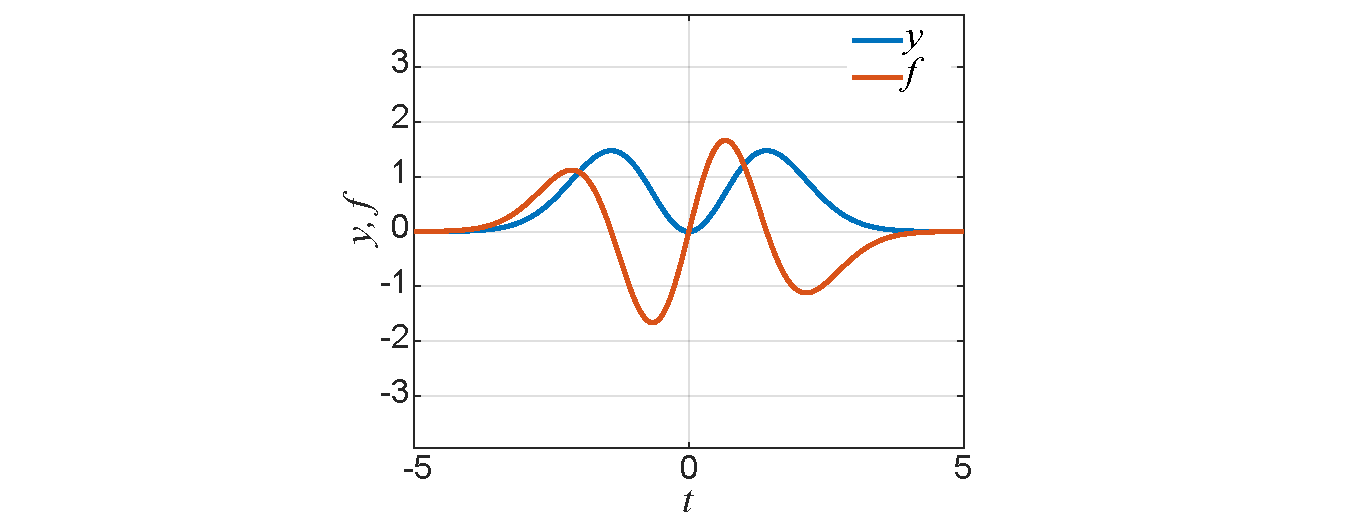
\includegraphics[width=\textwidth]{MatLabSymbolic.pdf}
\caption[Ergebnisfenster des \matlab-Programms f�r symbolische Berechnung.]{Ergebnisfenster des \matlab-Programms f�r eine symbolische Berechnung.}\label{abb:solman_matlab_symb}
\end{figure}

%-----------------------------------------------------------------------------------------------------------------------------------------------------------------------------
\section{Toolboxen}
Auch wenn es aus methodisch-didaktischer Sicht sinnvoll erscheint, sich seine eigenen Funktionsbibliotheken zu erstellen, muss das Rad nicht immer neu erfunden werden.
Die Basis-F�higkeiten von \matlab{} k�nnen n�mlich durch die Verwendung von vorkonfigurierten Toolboxen signifikant erweitert werden. Diese kuratierten Toolboxen m�ssen separat installiert werden. Toolboxen sind Bibliotheken von Skripten, die von der Firma Mathworks und Kooperationspartnern (\url{http://www.mathworks.com}) erstellt wurden, um bestimmte Problemgruppen zu l�sen. Derzeit sind \ua folgende Toolboxen verf�gbar, die f�r die Anwendungen in diesem Buch und in der CP relevant sind:
\begin{itemize}
	\item Symbolic Math Toolbox
	\item Mapping Toolbox
	\item Partial Differential Equation Toolbox
	\item Statistics and Machine Learning Toolbox
	\item Curve Fitting Toolbox
	\item Optimization Toolbox
	\item Image Processing Toolbox
	\item Verschiedene Toolboxen zur Physikalische Modellierung
\end{itemize}
Ausf�hrlichere Informationen zu diesen Toolboxen erhalten Sie unter \url{http://www.mathworks.com}.
Das Kommando \mlcmd{ver} listet zudem alle installierten Toolboxen und deren Versionsnummern auf.

\chapter{Verzeichnis der \mscre} \label{kap:solman_matlablist}

\subsection{\mscre -- Physik der Bewegung}\label{kap:bew_matlabskripts}

Die \mscre befinden sich im MATLAB-Ordner \texttt{MatlabDateien/bew},
die Hilfsfunktionen im dortigen Unterordner \texttt{Include\-folder} und Daten im Unterordner \texttt{Data}.
Es wird empfohlen, entweder die Skripte im GitHub Verzeichnis \githubSN zu benutzen oder sich die komplette Verzeichnisstruktur von \MKc~ runter zu laden und diese und auch das Arbeitsbuch im Hauptverzeichnis Fingeruebungen zu installieren. \\

Wir wollen noch einmal explizit darauf hinweisen, dass die \mscre prim�re der Vermittlung der physikalischen Modelle dienen und keinen Anspruch auf besonders elegante oder effiziente Programmierung erheben. Unser Buch ist ja kein Lehrbuch f�r \matlab-Programmierung. Uns ging es bewusst darum, dass die Skripte gut lesbar sind und das physikalische Modell bzw den physikalischen Gedankengang m�glichst klar abbilden.
Die Leser sind aufgerufen, die Programme nach Belieben zu verbessern und kompakter zu gestalten und diese auch ins GitHub Verzeichnis \githubSN zu stellen.

\subsubsection {Skripte zu Beispielen} \label{mls:bew_kapitel} 
\begin{longtable}{p{0.33\textwidth}p{0.67\textwidth}}
\hline\noalign{\smallskip}
Skript & Beschreibung \\
\noalign{\smallskip}\svhline\noalign{\smallskip}
%\href{bew/matlab/HarmonOszillator.m}{HarmonOszillator.m} & L�sung der Bewegungsgleichung f�r den getriebenen harmonischen Oszillator mit Reibung.\\

%\mlbewref{AchterbahnLoop.m}             & Durchlaufen einer kreisf�rmigen Loop auf einer Achterbahn (Einzelner Wagen und Zug im Vergleich).\\
\mlbewref{AnHarmonOszillator01.m}       & Schwingungsperiode f�r den anharmonischen Oszillator exakt und in verschiedenen N�herungen.\\
\mlbewref{AnHarmonOszillator02.m}       & L�sung der Bewegungsgleichung f�r den anharmonischen Oszillator in verschiedenen N�herungen.\\
\mlbewref{BungeeJumping.m}              & L�sung der Lagrange-Gleichungen f�r das Bungee-Jumping.\\
\mlbewref{Doppelkegel01.m}              & Herleitung der Lagrange-Gleichungen f�r den aufw�rts rollenden Doppelkegel aus der Lagrange-Funktion mittels der symbolischen Toolbox von \matlab.\\
\mlbewref{Doppelkegel02.m}              & L�sung der Lagrange-Gleichungen f�r den aufw�rts rollenden Doppelkegel.\\
\mlbewref{Doppelkegel03.m}              & Phasenraum des aufw�rts rollenden Doppelkegels aus der Energieerhaltung.\\
\mlbewref{Doppelkegel04.m}              & Phasenraum des aufw�rts rollenden Doppelkegels aus der Energieerhaltung f�r verschiedene Parameter.\\
\mlbewref{Doppelpendel01.m}             & Herleitung der Lagrange-Gleichungen f�r das Doppelpendel aus der Lagrange-Funktion mittels der symbolischen Toolbox von \matlab.\\
\mlbewref{Doppelpendel02.m}             & Beispielrechnungen und Simulation des Doppelpendels.\\
\mlbewref{FallendeKette.m}              & L�sung der Lagrange-Gleichungen f�r die fallende Kette.\\
\mlbewref{FallendeLeiter.m}             & Dynamik f�r eine fallende ("`wegrutschende"') Leiter.\\
\mlbewref{FallenderStab01.m}            & Kr�fteverh�ltnisse bei fallenden Stab.\\
\mlbewref{FallenderStab02.m}            & L�sung der Lagrange-Gleichungen f�r den fallenden Stab f�r verschiedene Reibungskoeffizienten.\\
\mlbewref{FoucaultPendel.m}             & Drehung der Schwingungsebene beim Foucault-Pendel.\\
\mlbewref{GekoppeltePendel01.m}         & Beispielrechnungen und Simulation der gekoppelten Pendel f�r gleiche Pendel, kleine Winkel.\\
\mlbewref{GekoppeltePendel02.m}         & Beispielrechnungen und Simulation der gekoppelten Pendel f�r unterschiedliche Pendel, kleine Winkel.\\
\mlbewref{GekoppeltePendel03.m}         & Beispielrechnungen und Simulation der gekoppelten Pendel f�r allgemeine Bedingungen, gro�e Winkel.\\
\mlbewref{Gyrotwister.m}                & Simulation der Beschleunigung des Kreisels im Gyrotwister durch die Bewegung der Hand.\\
\mlbewref{GyrotwisterPhase.m}           & Simulation der Beschleunigung des Kreisels im Gyrotwister durch die Bewegung der Hand bei einer Phasendifferenz zur optimalen Bewegung.\\
\mlbewref{HarmonOszillator.m}           & L�sung der Bewegungsgleichung f�r den getriebenen harmonischen Oszillator mit Reibung.\\
\mlbewref{Harpune.m}                    & L�sung der Lagrange-Gleichungen f�r einen senkrecht geworfenen Enterhaken/eine Harpune.\\
\mlbewref{JoJo01.m}                     & Berechnungen zur Dynamik eines Jo-Jos.\\
\mlbewref{KfKreiselFreieAchsen.m}       & Beispielrechnungen und Simulation zur Stabilit�t des kr�ftefreien Kreisels mit freien Achsen.\\
\mlbewref{KfSymmKreiselNutation.m}      & Beispielrechnungen zur Nutation des kr�ftefreien symmetrischen Kreisels im raumfesten System.\\
\mlbewref{Klothoide.m}                  & Berechnungen zur Klothoide (Cornu-Spirale) und Form eines Loopings f�r eine Achterbahn.\\
\mlbewref{KopPendelKleinWinkel.m}       & Beispielrechnungen und Simulation der gekoppelten Pendel f�r die Kleinwinklen�herung (analytische und numerische Rechnung).\\
\mlbewref{NLOszillator01.m}             & L�sung der Bewegungsgleichung f�r den getriebenen nichtlinearen Oszillator mit Reibung.\\
\mlbewref{NLOszillator02.m}             & Berechnung des Ljapunow-Exponenten f�r den getriebenen nichtlinearen Oszillator mit Reibung.\\
\mlbewref{Pendeluhr.m}                  & Berechnungen zur Pendeluhr.\\
\mlbewref{RollendesRad.m}               & Bewegung eines rollenden Rades.\\
\mlbewref{Rutherford.m}                 & Berechnungen zur Rutherford-Streuung.\\
\mlbewref{Schaukel01.m}                 & Berechnungen zur Dynamik einer Schaukel als parametrischen Oszillator.\\
\mlbewref{Schaukel02.m}                 & Berechnungen zur Dynamik einer Schaukel als getriebener Oszillator H�he.\\
\mlbewref{SchwererKreiselPraez01.m}     & Simulationsrechnung zur Pr�zession des schweren symmetrischen Kreisels im raumfesten System.\\
\mlbewref{SchwererKreiselPraez02.m}     & Beispielrechnungen zur Pr�zession des schweren symmetrischen Kreisels im raumfesten System.\\
\mlbewref{TrebSimDAE.m}                 & Berechnungen zur Dynamik eines \textit{Trebuchet}. Trebuchet mit Ber�cksichtigung von Zwangsbedingungen.\\
\mlbewref{TrebuchetSim02.m}             & Berechnungen zur Dynamik eines \textit{Trebuchet}. Modelle ohne Ber�cksichtigung der Zwangsbedingungen.\\
\mlbewref{TrebuchetLGL02.m}             & Symbolische Berechnung Lagrange-Funktion und Lagrange-Gleichungen f�r ein \textit{Trebuchet}.\\

\noalign{\smallskip}\svhline\noalign{\smallskip}
\end{longtable}

\newpage
\subsubsection{Skripte zu �bungen} \label{mls:bew_uebungen} %MLSkript�bungen
\begin{longtable}{p{0.33\textwidth}p{0.67\textwidth}}
\hline\noalign{\smallskip}
Skript & Beschreibung \\
\noalign{\smallskip}\svhline\noalign{\smallskip}
\mlbewref{AbplattungPlaneten.m}      & Berechnungen zur Abplattung der Planeten.\\
\mlbewref{Achterbahn01.m}            & Zeitliche Entwicklung eines Massepunktes auf einer Gau�-Kurve ($z = H\e^{-a^2 x^2}$) unter Einfluss der Gravitation.\\
\mlbewref{Achterbahn02.m}            & Zeitliche Entwicklung eines Massepunktes auf einer vorgegebenen Kurve ($z = 1+\tanh(x)$) unter Einfluss der Gravitation.\\
\mlbewref{Achterbahn03.m}            & Zeitliche Entwicklung der Bewegung eines Massepunktes auf einer parametrisierten Kurve (Trisectrix) unter Einfluss der Gravitation.\\
\mlbewref{Achterbahn04.m}            & Zug $N$ mit Federn gekoppelter Wagen auf einer Achterbahn in Form einer Gau�-Kurve.\\
\mlbewref{Achterbahn06.m}            & Zug $N$ mit Federn gekoppelter Wagen auf einer Achterbahn in Form eines Kreisloopings.\\
\mlbewref{AsteroidKollision.m}       & Kollisionswahrscheinlichkeit von Asteroiden mit Planeten.\\
\mlbewref{AsteroidStreuung.m}        & Berechnung von Trajektorien f�r Asteroiden in der Erdbahn.\\
\mlbewref{AsymmKreiselStab.m}        & Betrachtung zur Stabilit�t des asymmetrischen Kreisels, numerische L�sungen mittels \odevf.\\
\mlbewref{BallistikCoriolis01.m}     & Berechnung der Effekte der Coriolis-Kraft auf den freien Fall.\\
\mlbewref{BallistikCoriolis02.m}     & Berechnung der Effekte der Coriolis-Kraft auf die Ballistik eines Projektils, das nach S�den abgeschossen wird. Exakte L�sung.\\
\mlbewref{BallistikCoriolis03.m}     & Berechnung der Effekte der Coriolis-Kraft auf die Ballistik eines Projektils, das nach S�den abgeschossen wird. Die Reibung wird ber�cksichtigt. Numerische L�sung mittels \odevf.\\
\mlbewref{Baton.m}                   & Bewegungsgleichung Baton, numerische L�sung mittels \odevf. \\
\mlbewref{BaumgartnerFall.m}         & Freier Fall aus gro�er H�he (Baumgartner-Weltrekord).\\
\mlbewref{Billardspiel.m}            & Berechnung der Streuwinkel und Geschwindigkeiten beim Sto� zweier Billardkugeln.\\
\mlbewref{Brachistochrone.m}         & Berechnungen zur Brachistochrone und Tautochrone, sowie Lagrange-Funktion und  Lagrange Gleichungen des Zykloidenpendels.\\
\mlbewref{Doppelkegel05.m}           & Phasenraum und Dynamik des aufw�rts rollenden Doppelkegels (N�herung 1).\\
\mlbewref{Doppelkegel06.m}           & Phasenraum und Dynamik des aufw�rts rollenden Doppelkegels (N�herung 2).\\
\mlbewref{DoppelkegelVergleich.m}    & Vergleich der L�sungen f�r den aufw�rts rollenden Doppelkegel.\\
\mlbewref{ElastischerStoss.m}        & Berechnung des Energie�bertrag als Funktion des Streuwinkels im Laborsystem.\\
\mlbewref{EulerWinkel.m}             & Berechnung von Euler-Winkeln.\\
\mlbewref{Expander.m}                & Abh�ngigkeit der Schwingungsperiode von der Anfangsauslenkung eines intrinsisch nichtlinearen Oszillators am Beispiel eine Expanders.\\
\mlbewref{Gezeitenkraefte.m}         & Berechnet die Verformung eines Rings durch Gezeitenkr�fte.\\
\mlbewref{GekoppeltePendel01.m}      & L�sung der Bewegungsgleichung analytisch und numerisch f�r gekoppelte Stangenpendel (kleine Winkel, gleiche L�ngen). \\
\mlbewref{GekoppeltePendel02.m}      & L�sung der Bewegungsgleichung analytisch und numerisch f�r gekoppelte Stangenpendel (kleine Winkel, unterschiedliche L�ngen). \\
\mlbewref{GekoppeltePendel03.m}      & L�sung der Bewegungsgleichung mit/ohne Reibung f�r gekoppelte Stangenpendel (allgemeiner Fall). \\
\mlbewref{Hantelwurf.m}              & Berechnung der Bahn einer geworfenen Hantel als numerische L�sung mittels \odevf.\\
\mlbewref{HarmonOszQuadReibung.m}    & L�sung der Bewegungsgleichung f�r den harmonischen Oszillator mit Newton-Reibung.\\
\mlbewref{JoJo02.m}                  & Berechnungen zur Dynamik eine angetrieben Jo-Jos mit Reibung.\\
\mlbewref{KarussellCoriolis01.m}     & Berechnung der Effekte der Coriolis-Kraft auf einem gleichf�rmig rotierenden Karussell.\\
\mlbewref{KarussellCoriolis02.m}     & Berechnung der Effekte der Coriolis-Kraft auf einem beschleunigt rotierenden Karussell.\\
\mlbewref{Kettenfontaene.m}          & Programm berechnet den Z-Verlauf der Kettenfont�ne.\\
\mlbewref{KfSymmKreiselSimul.m}      & Simulationsrechnung der Nutation des kr�ftefreien symmetrischen Kreisels.\\
\mlbewref{KfKreiselDrehimpuls.m}     & Beispiele zur Simulation des allgemeinen kr�ftefreien Kreisels und seines Drehimpulses im k�rperfesten System.\\
\mlbewref{Kontraktion.m}             & Berechnungen zur Kontraktion und Energie einer rotierenden Galaxie.\\
\mlbewref{KopPendelKleinWinkel.m}    & Dynamik der gekoppelten Federpendel.\\
\mlbewref{KreiselKomp.m}             & Simulation des Einstellens der Nordrichtung beim fl�ssigkeitsged�mpften Kreiselkompass.\\
\mlbewref{KreiselKompMissweisung.m}  & Berechnung der Missweisung eines Kreiselkompasses bei Bewegung entlang eines L�ngenkreises.\\
\mlbewref{LagrangePunkte.m}          & Berechnung der Hill-Kurve und der Lagrange-Punkte.\\
\mlbewref{LogistischeGleichung01.m}  & Berechnung der Trajektorien der Logistischen Gleichung.\\
\mlbewref{LogistischeGleichung02.m}  & Bifurkationsgraph und Ljapunow-Exponent der Logistischen Gleichung.\\
\mlbewref{MolekuelPot.m}             & Simulation der Schwingungen eines zweiatomigen Molek�ls.\\
\mlbewref{MurphysLaw.m}              & Simulation zu Murphy's Law (Butterbrotscheiben-Versuch).\\
\mlbewref{PerleDraht.m}              & L�sung der Bewegungsgleichung ohne Reibung f�r die Perle auf Draht. \\
\mlbewref{PerleDrahtErweiterung.m}   & L�sung der Bewegungsgleichung mit Reibung f�r die Perle auf Draht mit verschiedenen Potentialen. \\
\mlbewref{Rollenpendel.m}            & L�sung der Bewegungsgleichung ohne Reibung f�r das Rollenpendel. \\
\mlbewref{RollenpendelReibung.m}     & L�sung der Bewegungsgleichung mit Reibung f�r das Rollenpendel.\\
\mlbewref{RollendesRad.m}            & Berechnung der Euler-Winkel und der Trajektorie einer Kreisscheibe \bzw eines Reifens auf einer ebenen Fl�che (ohne Reibung).\\
\mlbewref{RollendesRadR.m}           & Berechnung der Euler-Winkel und der Trajektorie einer Kreisscheibe \bzw eines Reifens auf einer ebenen Fl�che (mit Reibung).\\
\mlbewref{RutherfordAlpha.m}         & Trajektorienberechnung der Rutherford-Streuung von $\alpha$-Teilchen an Goldfolie.\\
\mlbewref{RutherfordAg.m}            & Trajektorienberechnung der Rutherford-Streuung von Silber-Teilchen an Goldfolie.\\
\mlbewref{SchaukelLG.m}              & Lagrange-Gleichung f�r die Schaukel mit sitzender und schwingender Person.\\
\mlbewref{Schaukel03.m}              & L�sung der DGL f�r die Schaukel mit Kette und verhindertem �berschlag.\\
\mlbewref{SchwererKreiselSim.m}      & Simulation der Figurenachse eines schweren Kreisels mit und ohne Nutation.\\
\mlbewref{Sinuslauf.m}               & Berechnung der Frequenz und Stabilit�t des Sinuslaufs bei starren Radachsen auf Schienen.\\
\mlbewref{Skydiver.m}                & Berechnung Fall aus gro�er H�he (Baumgartner-Weltrekord).\\
\mlbewref{SwingBy.m}                 & Berechnungen zum Swing- By am Jupiter.\\
\mlbewref{Tilgung01.m}               & Berechnung der Schwingungsd�mpfung in Hochh�usern.\\
\mlbewref{Tilgung02.m}               & Programm berechnet Frequenzantwort bei der Schwingungsd�mpfung an Hochh�usern.\\
\mlbewref{Tilgung03.m}               & Programm berechnet Frequenzantwort Schwingungsd�mpfung f�r Taipei 101 und den Berliner Fernsehturm.\\
\mlbewref{Traegheitsmomente.m}       & Berechnungen zu Tr�gheitsmomenten.\\
\mlbewref{TrebuchetLGL01.m}          & Lagrange-Funktion und Lagrange-Gleichungen f�r ein \textit{Trebuchet}.\\
\mlbewref{TrebuchetSim01.m}          & Berechnungen zur Dynamik des \textit{Trebuchet}.\\
\mlbewref{VibDaempfung01.m}          & Berechnung der Dynamik eines Sto�d�mpfers auf Basis Lagrange-Gleichungen.\\
\mlbewref{VibDaempfung02.m}          & Berechnung der D�mpfung einer Deckenaufh�ngung.\\
\mlbewref{Waschmaschine01.m}         & Berechnung des Schwingungs- und Resonanzverhaltens einer Trommelwaschmaschine in der Hochlaufphase.\\
\mlbewref{Waschmaschine02.m}         & Berechnung des Schwingungs- und Resonanzverhaltens einer Trommelwaschmaschine in der Auslaufphase.\\
\mlbewref{WeltraumFahrstuhl.m}       & Berechnungen zum Weltraumfahrstuhl.\\
\mlbewref{Wilberforce.m}             & Berechnung der Dynamik des linearen und nichtlinearen Wilberforce-Pendels auf Basis von Lagrange-Gleichungen (Resonanzfall).\\
\mlbewref{WurfmitohneReibung.m}      & Berechnung Auf- und Abstiegszeiten beim senkrechten Wurf mit und ohne Reibung.\\

\noalign{\smallskip}\hline\noalign{\smallskip}
\end{longtable}


\subsubsection {Hilfsfunktionen} \label{mls:bew_hilfsfunktionen} 

\begin{longtable}{p{0.33\textwidth}p{0.67\textwidth}}
\hline\noalign{\smallskip}
Skript & Beschreibung \\
\noalign{\smallskip}\svhline\noalign{\smallskip}
Mathematische Funktionen \\
\noalign{\smallskip}\svhline\noalign{\smallskip}
\mlbewiref{EulerLagrange.m}             & Symbolische Berechnung der Euler-Lagrange Gleichungen (\url{https://www.mathworks.com/matlabcentral/fileexchange/93275-euler-lagrange-solver}), MATLAB Central File Exchange. 27.12.2021, Copyright (c)  Morten Veng 2021.\\
\mlbewiref{Modulo.m}                    & Modulus-Funktion.\\
\mlbewiref{R\_x.m}, \mlbewiref{R\_y.m}, \mlbewiref{R\_z.m}     & Rotationsmatrizen bez�glich x,y,z-Achse.\\

\noalign{\smallskip}\svhline\noalign{\smallskip}
Hilfsfunktionen f�r Ein- und Ausgabe \\
\noalign{\smallskip}\svhline\noalign{\smallskip}
\mlbewiref{Ausgabewerte.m}              & Printfunktion f�r Ausgabewerte.\\
\mlbewiref{GetColorLines.m}             & L�dt Farbtabelle f�r Linien und graphische Darstellungen.\\
\mlbewiref{ImportFile01.m}              & Einlesen von Daten einer Matrix.\\ 
\mlbewiref{ImportFile02.m}              & Einlesen von Daten eines Text-Files.\\
\mlbewiref{LabelPoints.m}               & Beschriftung von Datenpunkten.\\
\mlbewiref{PlotCircle.m}	            & Graphische Ausgabe von Fr�hlingspunkt und Sonnen.\\
\mlbewiref{PlotTrebuchet.m}	            & Graphische Ausgabe der Geometrie eines Trebuchet.\\
\mlbewiref{StrDMS.m}                    & Umrechnung von Formaten f�r Ausgabe von Winkeln von Dezimal in Grad, Bogenminute, Bogensekunde.\\
\mlbewiref{StrHMS.m}                    & Umrechnung von Formaten f�r Ausgabe von Zeit von Dezimal in hh:mm:ss.s.\\
\noalign{\smallskip}\svhline\noalign{\smallskip}
\end{longtable}


 
\clearpage
\subsection{\mscre -- Physik des Kontinuums}\label{kap:kontmech_matlabskripts}

Die \mscre befinden sich im MATLAB-Ordner \texttt{MatlabDateien/kontmech},
die Hilfsfunktionen im dortigen Unterordner \texttt{Include\-folder} und Daten im Unterordner \texttt{Data}.
Es wird empfohlen, entweder die Skripte im GitHub Verzeichnis \githubSN zu benutzen oder sich die komplette Verzeichnisstruktur von \MKc~ runter zu laden und diese und auch das Arbeitsbuch im Hauptverzeichnis Fingeruebungen zu installieren. \\

Wir wollen noch einmal explizit darauf hinweisen, dass die \mscre prim�re der Vermittlung der physikalischen Modelle dienen und keinen Anspruch auf besonders elegante oder effiziente Programmierung erheben. Unser Buch ist ja kein Lehrbuch f�r \matlab-Programmierung. Uns ging es bewusst darum, dass die Skripte gut lesbar sind und das physikalische Modell bzw den physikalischen Gedankengang m�glichst klar abbilden.
Die Leser sind aufgerufen, die Programme nach Belieben zu verbessern und kompakter zu gestalten und diese auch ins GitHub Verzeichnis \githubSN zu stellen.


%\begin{prob}\label{mls:kontmech_hilfsfunktionen} %MLSkript1 
%\textbf{Hilfsfunktionen} \\
%\begin{longtable}{p{0.33\textwidth}p{0.67\textwidth}}
%\hline\noalign{\smallskip}
%Skript & Beschreibung \\
%\noalign{\smallskip}\svhline\noalign{\smallskip}
%Mathematische Funktionen \\
%\noalign{\smallskip}\svhline\noalign{\smallskip}
%\mlkontmechref{Beispiel.m} & Ein Beispieltext.\\
%\noalign{\smallskip}\svhline\noalign{\smallskip}
%\end{longtable}
%\end{prob}

\subsubsection {Skripte zu Beispielen} \label{mls:kontmech_kapitel} 
\begin{longtable}{p{0.33\textwidth}p{0.67\textwidth}}
\hline\noalign{\smallskip}
Skript & Beschreibung \\
\noalign{\smallskip}\svhline\noalign{\smallskip}
\mlkontmechref{SchwingendeSaite01.m} & L�sen der Differentialgleichung einer
schwingenden Saite f�r eine stehende Welle.\\
\noalign{\smallskip}\svhline\noalign{\smallskip}
\end{longtable}

\subsubsection {Skripte zu �bungen} \label{mls:kontmech_uebungen} 
\begin{longtable}{p{0.33\textwidth}p{0.67\textwidth}}
\hline\noalign{\smallskip}
Skript & Beschreibung \\
\noalign{\smallskip}\svhline\noalign{\smallskip}
\mlkontmechref{AchterbahnKont.m}        & L�sen der Differentialgleichung eines kontinuierlichen, elastischen Achterbahnzuges auf einer Gau�kurven-Strecke.\\
\mlkontmechref{AchterbahnKontBeschl.m}  & Normalbeschleunigung auf einen Fahrgast im kontinuierlichen, elastischen Achterbahnzug.\\
\mlkontmechref{Chladni01.m}             & L�sen der Eigenschwingungen einer kreisf�rmigen, elastischen Fl�che.\\
\mlkontmechref{Chladni02.m}             & L�sen der Eigenschwingungen einer quadratischen, elastischen Fl�che.\\
\mlkontmechref{Chladni03.m}             & L�sen der Eigenschwingungen einer rechteckigen, elastischen Fl�che.\\
\mlkontmechref{Divergenz.m}             & Programm berechnet Vektorfunktionen und ihre Divergenz.\\
\mlkontmechref{FassFormelGauss.m}       & Programm berechnet Volumen von Rotationsk�rpern �ber Gau�schen Integralsatz.\\
\mlkontmechref{GespannterBogen.m}       & L�sen der Eigenschwingungen eines Bogens, der durch eine Saite gespannt ist.\\
\mlkontmechref{GradientFunktion1.m}     & Programm berechnet Funktionen und ihre Gradienten.\\
\mlkontmechref{GradientFunktion2.m}     & Programm berechnet Funktionen und ihre Gradienten (Yukawa-Potential).\\
\mlkontmechref{GradientFunktion3.m}     & Programm berechnet Funktionen und ihre Gradienten (Kepler-Potential mit Drehimpuls).\\
\mlkontmechref{KdVTsunami.m}            & Berechnung eines KdV-Solitons, das auf eine K�ste zul�uft, an der die Wassertiefe abnimmt.\\
\mlkontmechref{KdV01.m}                 & L�sen der Korteweg-de-Vries-Gleichung f�r ein einzelnes Soliton.\\
\mlkontmechref{KdV02.m}                 & Vergleich mehrerer Solitonen der KdV-Gleichung mit unterschiedlicher Geschwindigkeit.\\
\mlkontmechref{KdV03.m}                 & Summen aus einzelnen Solitonen in der KdV-Gleichung.\\
\mlkontmechref{KdV04.m}                 & Interaktion von Solitonen in der KdV-Gleichung.\\
\mlkontmechref{Kreisrohr.m}             & Berechnen des Geschwindigkeitsprofils einer station�ren Str�mung in einem kreisrunden Rohr.\\
\mlkontmechref{NLSGSolitonen.m}         & L�sen der nichtlinearen Schr�dinger-Gleichung f�r ein Soliton.\\
\mlkontmechref{Rechteckrohr.m}          & Berechnen des Geschwindigkeitsprofils einer station�ren Str�mung in einem rechteckigen Rohr.\\
\mlkontmechref{Rotation.m}              & Programm berechnet Vektorfunktionen und ihre Rotation.\\
\mlkontmechref{SchwingendeSaite02.m}    & L�sen der Differentialgleichung einer eingespannten Saite f�r eine Gau�sche St�rung.\\
\mlkontmechref{SchwingendeSaite03.m}    & L�sen der Differentialgleichung einer eingespannten Saite f�r eine einseitig angeregte Welle.\\
%\noalign{\smallskip}\svhline\noalign{\smallskip}
\mlkontmechref{SinusGordonSolitonen.m}  & L�sen der Sinus-Gordon-Gleichung f�r ein Soliton.\\
\mlkontmechref{Tank.m}  & Fluss durch einen quadratischen Tank mit zwei �ffnungen.\\
\mlkontmechref{Torricelli.m}  & Fluss einer Fl�ssigkeit aus einem Tank nach dem
Gesetz von Torricelli.\\
\end{longtable}



 
\clearpage
\subsection{\mscre--Himmelsmechanik}\label{kap:hm_matlabskripts}

Die \mscre befinden sich im MATLAB-Ordner \texttt{MatlabDateien/hm},
die Hilfsfunktionen im dortigen Unterordner \texttt{Include\-folder} und Daten im Unterordner \texttt{Data}.

Die \mscre befinden sich im MATLAB-Ordner \texttt{MatlabDateien/hm},
die Hilfsfunktionen im dortigen Unterordner \texttt{Include\-folder} und Daten im Unterordner \texttt{Data}.
Es wird empfohlen, entweder die Skripte im GitHub Verzeichnis \githubSN zu benutzen oder sich die komplette Verzeichnisstruktur von \MKc~ runter zu laden und diese und auch das Arbeitsbuch im Hauptverzeichnis Fingeruebungen zu installieren. \\

Wir wollen noch einmal explizit darauf hinweisen, dass die \mscre prim�re der Vermittlung der physikalischen Modelle dienen und keinen Anspruch auf besonders elegante oder effiziente Programmierung erheben. Unser Buch ist ja kein Lehrbuch f�r \matlab-Programmierung. Uns ging es bewusst darum, dass die Skripte gut lesbar sind und das physikalische Modell bzw den physikalischen Gedankengang m�glichst klar abbilden.
Die Leser sind aufgerufen, die Programme nach Belieben zu verbessern und kompakter zu gestalten und diese auch ins GitHub Verzeichnis \githubSN zu stellen.

\subsubsection{Skripte zu Beispielen}\label{mls:hm_bsp_uebungen} %MLSkript1 

\subparagraph{\textbf{Exzentrizit�t Planetenbahnen}}\label{mls:hm_exzentri} %MLSkript2
\begin{longtable}{p{0.33\textwidth}p{0.67\textwidth}}
\hline\noalign{\smallskip}
Skript & Beschreibung \\
\noalign{\smallskip}\svhline\noalign{\smallskip}
\mlhmref{PlanetExzentrizitaeten.m}	& Darstellung der Exzentrizit�ten der Planetenbahnen (auf gro�e Halbachse $a$ normiert).\\
\noalign{\smallskip}\hline\noalign{\smallskip}
\end{longtable}

\subparagraph{\textbf{Analemma}}\label{mls:hm_analemma} %MLSkript3
\begin{longtable}{p{0.33\textwidth}p{0.67\textwidth}}
\hline\noalign{\smallskip}
Skript & Beschreibung \\
\noalign{\smallskip}\svhline\noalign{\smallskip}
\mlhmref{Analemma01.m}        & Analemma auf Basis einer auf der Mittelpunktsgleichung basierenden Keplerl�sung f�r die Sonnenbahn. Exzentrizit�t und Ekliptikschiefe werden variiert (�quinoktium und Ekliptik des Datums). \\
\mlhmref{Analemma02.m}        & Analemmaberechnung (N�herungsrechnung) f�r verschiedene geographische Positionen in Alt-Azimut-Darstellung f�r 24 h. Refraktion und Tagbogenverl�ngerung vernachl�ssigt. Es wird eine einfache auf der Mittelpunktsgleichung basierenden Keplerl�sung f�r die Erdbahn benutzt (�quinoktium und Ekliptik des Datums). \\
\mlhmref{Analemma03.m}        & Analemmaberechnung f�r verschiedene Planeten direkt aus der exzentrischen Anomalie $E$ ohne L�sung der Kepler-Gleichung.\\
\mlhmref{AnalemmaSonne.m}  & Analemmaberechnung der Sonne vom Mond aus auf Basis von auf der Mittelpunktsgleichung basierenden Keplerl�sungen f�r die Sonnen- und Mondbahn.\\
\mlhmref{AnalemmaMond.m}    & Analemmaberechnung f�r Mond von der Erde aus betrachtet auf Basis von auf der Mittelpunktsgleichung basierenden Keplerl�sungen f�r die Sonnen- und Mondbahn.\\
\mlhmref{AnalemmaOkoFit.m}    & Umrechnung einschlie�lich Bildkorrektur des aufgenommenen Analemma von Oberkochen 2019/20 in das horizontale KOS, sowie Darstellung verschiedener theoretisch berechneter Analemma. \\
\mlhmref{AnalemmaFindExz.m}   & Umrechnung einschlie�lich Bildkorrektur des aufgenommenen Analemma von Oberkochen 2019/20 in das horizontale KOS, sowie Fit eines theoretisch berechneten Analemmas mit der Exzentrizit�t e als Parameter. \\
\noalign{\smallskip}\hline\noalign{\smallskip}
\end{longtable}

\subparagraph{\textbf{Sonnenaufgangsberechnung (Methode der quadratischen Interpolation)}}\label{mls:hm_sonnenaufgang} %MLSkript4
\begin{longtable}{p{0.33\textwidth}p{0.67\textwidth}}
\hline\noalign{\smallskip}
Skript & Beschreibung \\
\noalign{\smallskip}\svhline\noalign{\smallskip}
\mlhmref{Sonnenaufgang01.m} & Aufgangs- und Untergangszeiten der Sonne f�r verschiedene geographische Orte (Breite < 60�) und die Tagl�ngen
 iterativ aus der Kepler-Gleichung f�r das ganze Jahr und in der N�he des Jahreswechsels bzw. Mitsommers.\\
\mlhmref{Sonnenaufgang02.m} & Aufgangszeiten auf Basis der Kepler-Gleichung  a) mit einer iterativen Methode (Quadratische 
Interpolation) zur Suche der Nullstellen f�r Auf- und Unterg�nge und b) zum Vergleich auf Basis der ZGL-N�herung.\\
\noalign{\smallskip}\hline\noalign{\smallskip}
\end{longtable}

\subparagraph{\textbf{Vergleich Zeitgleichung}}\label{mls:hm_zeitglgformeln} %MLSkript5
\begin{longtable}{p{0.33\textwidth}p{0.67\textwidth}}
\hline\noalign{\smallskip}
Skript & Beschreibung \\
\noalign{\smallskip}\svhline\noalign{\smallskip}
\mlhmref{ZGL01.m} & ZGL auf Basis einer Mittelpunktsgleichung basierenden Keplerl�sung f�r die Sonnenbahn und Vergleich mit empirischen Werten und den Berechnungen des JPL (�quinoktium und Ekliptik des Datums). \\
\mlhmref{ZGL02.m} & Reihenentwicklung der ZGL.\\
\mlhmref{ZGL03.m} & ZGL auf Basis einer (auf der Mittelpunktsgleichung basierten) Keplerl�sung f�r die Erdbahn und Vergleich mit verschiedenen publizierten N�herungsformeln und den Berechnungen des JPL. \\
\noalign{\smallskip}\hline\noalign{\smallskip}
\end{longtable}
 
\subparagraph{\textbf{Tagbogen-Verl�ngerung}}\label{mls:hm_tagbogenverl} %MLSkript6
\begin{longtable}{p{0.33\textwidth}p{0.67\textwidth}}
\hline\noalign{\smallskip}
Skript & Beschreibung \\
\noalign{\smallskip}\svhline\noalign{\smallskip}
\mlhmref{TagbogenVerlaengerung.m} & Tagbogenverl�ngerung bedingt durch Refraktion und scheinbaren Sonnendurchmesser bei Sonnenaufgang.\\
\noalign{\smallskip}\hline\noalign{\smallskip}
\end{longtable}

%\newpage
\subparagraph{\textbf{Tageslauf Sonne}}\label{mls:hm_tageslauf_sonne} %MLSkript7
\begin{longtable}{p{0.33\textwidth}p{0.67\textwidth}}
\hline\noalign{\smallskip}
Skript & Beschreibung \\
\noalign{\smallskip}\svhline\noalign{\smallskip}
\mlhmref{TageslaufSonne01.m} & Der Tageslauf der Sonne wird nach der N�herungsformel (3.84) berechnet. Die geographische Breite kann variiert werden. Es wird die H�he der Sonne f�r verschieden Jahreszeiten und geographische Breiten dargestellt. Die ZGL wird nicht ber�cksichtigt.
Berechnung des Tagbogenverlaufs (N�herung) der Sonne �ber dem Horizont f�r verschiedene Jahreszeiten und geographische Breiten.\\
\mlhmref{TageslaufSonne02.m} & Tagbogenverlauf der Sonne �ber dem Horizont. (N�herungsformel und zum numerische L�sung. Die geographische Breite kann variiert werden.\\
\noalign{\smallskip}\hline\noalign{\smallskip}
\end{longtable}
 


\subparagraph{\textbf{Berechnung der Aufgangswinkel der Sonne (Verschiedene Orte und Jahreszeiten)}}\label{mls:hm_aufgangswinkel_sonne} %MLSkript8
\begin{longtable}{p{0.33\textwidth}p{0.67\textwidth}}
\hline\noalign{\smallskip}
Skript & Beschreibung \\
\noalign{\smallskip}\svhline\noalign{\smallskip}
\mlhmref{SonnenaufgangZeit.m}    & H�he $h$ und Azimut $\mathcal{A}$ und die Zeit-H�hen-Kurven beim Sonnenaufgang auf Basis einer MPG-Keplerl�sung f�r verschiedene geographische Breiten und verschiedene Jahreszeiten (Wintersonnenwende, Fr�hlingsanfang, Sommersonnenwende, Herbstanfang). Dabei wird die astrometrische H�he $h$ und die durch Refraktion \ua Effekte bedingte \anf{scheinbare} H�he $h'$ berechnet.\\ 
\mlhmref{SonnenaufgangBaabe.m}        & H�he $h$ und Azimut $\mathcal{A}$ und die Zeit-H�hen-Kurven beim Sonnenaufgang auf Basis einer MPG-Keplerl�sung f�r die Erdbahn f�r Baabe (Ostsee). Dabei wird die astrometrische H�he $h$ und die durch Refraktion \ua Effekte bedingte \anf{scheinbare} H�he $h'$ berechnet.\\
\noalign{\smallskip}\hline\noalign{\smallskip}
\end{longtable}
 

\subparagraph{\textbf{Innere Planetenbahnen}}\label{mls:hm_innere_planeten} %MLSkript9
\begin{longtable}{p{0.33\textwidth}p{0.67\textwidth}}
\hline\noalign{\smallskip}
Skript & Beschreibung \\
\noalign{\smallskip}\svhline\noalign{\smallskip}
\mlhmref{InnerePlaneten.m} & Bahnen der inneren Planeten auf Basis der Kepler-Geichung. 
(�quinoktium und Ekliptik des Datums) \\
\mlhmref{VenusTransit01.m} & Koordinaten der Venus und des Merkurs bei Transits. Die Zeiten m�ssen n�herungsweise z.\,B. aus \mlhmref{InnerePlaneten.m} bekannt sein. Die Daten werden mit JPL-Daten verglichen. \\
\mlhmref{VenusTransit02.m} & Bestimmung der Astronomischen Einheit aus den Daten eines Venustransits. a) Parallaxen-Methode nach Halley: Die beobachteten Werte f�r zwei geographische Orte zu einer Zeit UT werden dem Internet entnommen, daraus wird die Parallaxe bestimmt und daraus dann die AE berechnet.  b) Kontaktzeitmethode durch Beobachtung an einem Standort.\\
\noalign{\smallskip}\hline\noalign{\smallskip}
\end{longtable}

\subparagraph{\textbf{�u�ere Planetenbahnen}}\label{mls:hm_aussere_planeten} %MLSkript10
\begin{longtable}{p{0.33\textwidth}p{0.67\textwidth}}
\hline\noalign{\smallskip}
Skript & Beschreibung \\
\noalign{\smallskip}\svhline\noalign{\smallskip}
\mlhmref{AeusserePlaneten.m} & Bahnen der �u�eren Planeten auf Basis der Kepler-Gleichung f�r den Zeitraum 1920--2020. (�quinoktium und Ekliptik des Datums) \\
\noalign{\smallskip}\hline\noalign{\smallskip}
\end{longtable}
 
\subparagraph{\textbf{St�rungsrechnung }}\label{mls:hm_stoerunsgrechnung_planeten} %MLSkript11
\begin{longtable}{p{0.33\textwidth}p{0.67\textwidth}}
\hline\noalign{\smallskip}
Skript & Beschreibung \\
\noalign{\smallskip}\svhline\noalign{\smallskip}
\mlhmiref{VenusExakt.m} & Ekliptikale Koordinaten der Venus auf Basis einer Reihenentwicklung \cite{Montenbruck1999}. \\
\mlhmiref{MarsExakt.m} & Ekliptikale Koordinaten des Mars auf Basis einer Reihenentwicklung \cite{Montenbruck1999}. \\
\mlhmiref{JupiterExakt.m} & Ekliptikale Koordinaten des Jupiters auf Basis einer Reihenentwicklung \cite{Montenbruck1999}. \\
\mlhmiref{SonneExakt.m}  & Ekliptikale Koordinaten der Sonne auf Basis der Newcombschen Theorie \cite{Montenbruck1999}. \\
\mlhmiref{MondExakt.m}. & Geozentrisch-�quatoriale Koordinaten des Mondes auf Basis der Brownschen Theorie \cite{Montenbruck1999}. \\
\mlhmref{SL9numerisch.m} & Bahn des Kometen Shoemaker-Levy 9 bis zu seinem Zusammenprall mit dem Jupiter �ber numerische Integration.
\end{longtable}


\subparagraph{\textbf{Periheldrehung des Merkurs}}\label{mls:hm_perihel_merkur} %MLSkript12
\begin{longtable}{p{0.33\textwidth}p{0.67\textwidth}}
\hline\noalign{\smallskip}
Skript & Beschreibung \\
\noalign{\smallskip}\svhline\noalign{\smallskip}
\mlhmref{PerihelKappa2.m}    & Perihel-Verschiebung f�r ein Potential mit Term $\kappa_2 \neq 0$. \\
\mlhmref{PerihelKappa3.m}    & Perihel-Verschiebung f�r ein Potential mit Term $\kappa_3 \neq 0$. \\
\mlhmref{StoerpotentialMerkur.m}  & St�rpotentiale und Gravitationskr�fte der anderen Planeten auf den Merkur als Ursache der Perihel-Verschiebung des Merkurs nach der Newtonschen Mechanik. \\
\noalign{\smallskip}\hline\noalign{\smallskip}
\end{longtable}

\subparagraph{\textbf{Kometenbahnen}}\label{mls:hm_kometenbahnen} %MLSkript13
\begin{longtable}{p{0.33\textwidth}p{0.67\textwidth}}
\hline\noalign{\smallskip}
Skript & Beschreibung \\
\noalign{\smallskip}\svhline\noalign{\smallskip}
\mlhmref{AsteroidenBahnen.m}   & Bahnen der Asteroiden in heliozentrischen Koordinaten unter Benutzung der Gau�schen Vektoren (�quinoktium und Ekliptik des Datums). \\
\mlhmref{AsteroidenZeit.m}     & Bahn eines Asteroiden als Funktion der Zeit unter fallweiser Benutzung einer parabolischen N�herung. (�quinoktium und Ekliptik des Datums). \\
\mlhmref{KometenBahnen.m}      & Bahnen der Kometen in heliozentrischen Koordinaten unter Benutzung der Gau�schen Vektoren (�quinoktium und Ekliptik des Datums).\\
\mlhmref{KometenZeit.m}        & Bahn eines Kometen als Funktion der Zeit unter fallweiser Benutzung einer parabolischen N�herung (�quinoktium und Ekliptik des Datums). \\
\mlhmref{KometenObsEqu.m}      & Kometenbahnen in Erdn�he als Funktion der Zeit und die Beobachtungsdaten (Rektaszension und Deklination) unter Benutzung von parabolischen N�herungen.\\
\mlhmref{KometenObsHor.m}      & Kometenbahnen in Erdn�he als Funktion der Zeit und die Beobachtungsdaten (Azimut und H�he) unter Benutzung von parabolischen N�herungen.\\
\mlhmref{KometenSL9.m}         & Kepler-Bahn des Kometen D/1993 F2-D (Shoemaker-Levy 9) als Funktion der Zeit und Vergleich mit Werten des JPL \cite{JPL2020} (�quinoktium und Ekliptik des Datums). \\
\mlhmref{KometenHalley.m}      & Bahnen des Kometen Halley von 1986 und 1758 (�quinoktium und Ekliptik Datums). \\
\noalign{\smallskip}\hline\noalign{\smallskip}
\end{longtable}

\subparagraph{\textbf{Gezeiten}}\label{mls:hm_gezeiten} %MLSkript13
\begin{longtable}{p{0.33\textwidth}p{0.67\textwidth}}
\hline\noalign{\smallskip}
Skript & Beschreibung \\
\noalign{\smallskip}\svhline\noalign{\smallskip}
\mlhmref{Gezeitenellipsoid.m}  & Berechnet die Form des Gezeitenellipsoids. \\
\mlhmref{GezeitenReibung01.m}  & Berechnet Parameter der Gezeitenreibung auf der Erde. \\
\mlhmref{GezeitenReibung02.m}  & Berechnet Parameter der Gezeitenreibung auf der Erde mit einem einfachen Hantelmodell.\\
\mlhmref{UmlaufErdeMond.m}     & Simuliert die Bewegung von Erde und Mond um gemeinsamen Schwerpunkt im Laufe eines Monats.\\
%\mlhmref{GezeitenDGLSystem.m}  & L�st das DGLS-System f�r ZKP inklusive Gezeitenreibung.\\
\mlhmref{SimulationAiry.m}     & Simuliert stehende Wellen nach dem Airy-Modell.\\
\noalign{\smallskip}\hline\noalign{\smallskip}
\end{longtable}


\subparagraph{\textbf{Sonnenfinsternisse}} \label{mls:hm_so_fis} %MLSkript14
\medskip
Diese Programme wurden in Teilen auf Basis der C++ Programmstrukturen und der Beschreibung/Erl�uterung in  
"Astronomie mit dem Personal Computer" von Oliver Montenbruck und Thomas Pfleger \cite{Montenbruck1999} entwickelt. 
Genehmigung des Verlages und der Autoren liegt vor.
\begin{longtable}{p{0.33\textwidth}p{0.67\textwidth}}
\hline\noalign{\smallskip}
Skript & Beschreibung \\
\noalign{\smallskip}\svhline\noalign{\smallskip}
\mlhmref{Sonnenfinsternis01.m}    & Zeiten des Neu/Vollmondes in einem bestimmten Zeitraum und bestimmt, ob zu der Neumond/Vollmondzeit eine Sonnen- oder Mondfinsternis stattfinden kann. F�r die Koordinaten Sonne und Mond werden genauere Reihen verwendet. \\
%\mlhmref{PhaseFunc.m} 	& Hilfsfunktion zur Berechnung der Zeiten des Neu/Vollmondes und von Finsternissen.\\
\mlhmref{Sonnenfinsternis02.m}    &  Startet von ungef�hren Neumondzeiten und bestimmt, wann und wo um die Neumondzeit eine Sonnenfinsternis stattfinden kann. F�r die Sonnenfinsternis wird die Zentrallinie der sogenannten maximalen Verfinsterung berechnet.\\
\mlhmref{Sonnenfinsternis03.m}    &  Bestimmt ausgehend vom Neumondzeitpunkt f�r einen gew�hlten Beobachtungsort die Phase, Gr��e und Kontaktzeiten einer Sonnenfinsternis.\\
\noalign{\smallskip}\hline\noalign{\smallskip}
\end{longtable}
 
\subparagraph{\textbf{Lange Zeiten}}\label{mls:hm_lange_zeiten} %MLSkript15
\begin{longtable}{p{0.33\textwidth}p{0.67\textwidth}}
\hline\noalign{\smallskip}
Skript & Beschreibung \\
\noalign{\smallskip}\svhline\noalign{\smallskip}
\mlhmref{ZGL04.m} & Zeitgleichung und Analemma �ber Zeitr�ume von mehreren Jahrtausenden. \\
\noalign{\smallskip}\hline\noalign{\smallskip}
\end{longtable}

\medskip
\subsubsection{Skripte zu verschiedenen �bungen}\label{mls:hm_uebungen} %MLSkript�bungen
\begin{longtable}{p{0.33\textwidth}p{0.67\textwidth}}
\hline\noalign{\smallskip}
Skript & Beschreibung \\
\noalign{\smallskip}\svhline\noalign{\smallskip}
\mlhmref{AbflachungSonne.m}         & Abflachung der Sonne bei Sonnenuntergang als Funktion der H�he.\\
\mlhmref{AnalemmaAnomalie.m}      & Zeitgleichung und Analemma direkt aus der exzentrischen Anomalie.\\
\mlhmref{AufprallgeschwindigkeitKomet.m}        & Aufprallgeschwindigkeit von Kometen/Meteoriten auf der Erde als Funktion verschiedener Parameter.\\
\mlhmref{Besselreihe.m}         & Bessel-Reihe f�r exzentrische Anomalie $E$ f�r verschiedene Exzentrizit�ten $e$ und Summationsgrenzen.\\
\mlhmref{KeplerVergleich.m}         & L�sung der Kepler-Gleichung �ber verschiedene Iterationsverfahren f�r verschiedene Exzentrizit�ten zwischen 0.1, 0.2,.....0.999. Vergleich der Iteration mit Regula falsi und Newton-Raphson f�r verschiedene Anfangswerte der mittleren Anomalie M.\\
\mlhmref{LangzeitJahreszeiten.m}         & Dauer der Jahreszeiten und Energieeintrag der Sonne auf die Nordhemisph�re f�r einen Zeitraum von 8000 Jahren. Einfache Modellierung der Ver�nderungen von Exzentrizit�t, Ekliptikneigung und Richtung der Erdachse.\\
\mlhmref{Mondbahn01.m}         & Mondbahn f�r ein einfaches koplanares ZK-Planet-Mond-System bezogen auf den Zentralk�rper f�r verschiedene Verh�ltnisse der Umlaufzeiten TM (Mond um Planet) und TP (Planet um ZK). \\
\mlhmref{Mondbahn02.m}         & Heliozentrische Mondbahn aus den Ephemeriden.\\
\mlhmref{MarsOpposition.m}         & Marsoppositionen im Zeitraum 2000--2020.\\
\mlhmref{MondErdeSonneApollo8.m}        & Programm berechnet die Positionen von Mond, Erde, Sonne und Apollo 8 am 24.12.1968.\\
\mlhmref{OlympusMons.m}         & Sonnenaufgang auf dem Mars.\\
\mlhmref{PlanetenbahnenKepler.m}         & Bahnen der Planeten Venus bis Jupiter auf Basis der Kepler-Gleichung. Venus-Jupiter-Konjunktion f�r den 22.\ 11.\ 2065 die  (�quinoktium und Ekliptik des Datum). \\
\mlhmref{Refraktion.m}         & Refraktionsberechnung f�r das Kugelschalen-Schichtenmodell und Vergleich mit der Normalrefraktion.\\
\mlhmref{RocheLimit.m}         & Berechnet Roche-Limit und Hill-Sph�ren f�r Planeten unseres Sonnensystems.\\
\mlhmref{SonnenaufgangReinsch.m}         & Analytische Formel f�r Sonnenaufgang nach \cite{Reinsch2003} und Vergleich mit numerischer Berechnung.\\
\mlhmref{SonnenuhrAnalem.m}  & Berechnet Lineatur einer analemmatischen Sonnenuhr f�r G�rlitz.\\
\mlhmref{SimulationAiry.m}  & Simuliert das Airy-Kanal-Modell der dynamischen Theorie der Gezeiten.\\
\mlhmref{TageslaufSonne.m}         & Tageslauf der Sonne mit Ber�cksichtigung der Refraktion $R$ und �ber den Tag ver�nderlicher Deklination $\delta$.\\
\mlhmref{VenusMerkurTransit.m}         & Venustransits am 08.06.2004 und am 06.06.2012.\\
\mlhmref{VerweildauerKomet.m}        & Verweildauer von Kometen in Erdn�he.\\
\mlhmref{Wandsonnenuhr.m}    & Berechnet Lineatur einer Wandsonnenuhr.\\
\mlhmref{ZGLAnalemma.m}      & Zeitgleichung und Analemma auf anderen Planeten (Methode Allison).\\
\mlhmref{ZGLAnalemmaKepler.m}      & Zeitgleichung und Analemma auf anderen Planeten (Methode Montenbruck).\\
\noalign{\smallskip}\hline\noalign{\smallskip}
\end{longtable}

%\newpage
\subsubsection{Hilfsfunktionen}\label{mls:hm_hilfsfunktionen} %MLSkript1 
Einige der Programme wurden in Teilen mit freundlicher Genehmigung der Autoren auf Basis der C++ Programmstrukturen und der Beschreibung/Erl�uterung in \glqq Astronomie mit dem Personal Computer\grqq{} von Oliver Montenbruck und Thomas Pfleger \cite{Montenbruck1999} entwickelt.\\
\begin{longtable}{p{0.33\textwidth}p{0.67\textwidth}}
\hline\noalign{\smallskip}
Skript & Beschreibung \\
\noalign{\smallskip}\svhline\noalign{\smallskip}
Mathematische Funktionen \\
\noalign{\smallskip}\svhline\noalign{\smallskip}
\mlhmiref{CalcAnglesfromXYZ.m}         & Sph�rische Koordinaten aus kartesischen Koordinaten.\\
\mlhmiref{CalcXYZfromAngles.m}         & Kartesische Koordinaten aus sph�rischen Koordinaten.\\
\mlhmiref{Frac.m}                      & Nachkommastellen.\\
\mlhmiref{Modulo.m}                    & Modulus-Funktion.\\
\mlhmiref{R\_x.m}, \mlhmiref{R\_y.m}, \mlhmiref{R\_z.m},     & Rotationsmatrizen bez�glich x,y,z-Achse.\\
\mlhmiref{Stumpff.m}                   & Stumpffsche Funktionen.\\
\noalign{\smallskip}\svhline\noalign{\smallskip}
Hilfsfunktionen f�r Ein- und Ausgabe \\
\noalign{\smallskip}\svhline\noalign{\smallskip}
\mlhmiref{GetColorLines.m}             & L�dt Farbtabelle f�r Linien und graphische Darstellungen.\\
\mlhmiref{StrDMS.m}                    & Umrechnung von Formaten f�r Ausgabe von Winkeln von Dezimal in Grad, Bogenminute, Bogensekunde.\\
\mlhmiref{HMS.m}                       & Umrechnung von Formaten f�r Zeit von Dezimal in hh:mm:ss.s \\
\mlhmiref{StrHMS.m}                    & Umrechnung von Formaten f�r Ausgabe von Zeit von Dezimal in hh:mm:ss.s \\
\mlhmiref{LabelPoints.m}               & Beschriftung von Datenpunkten.\\
\mlhmiref{OrbitParameter.m}            & Einlesen der Bahnparameter der Planeten.\\ 
\mlhmiref{KometParameter.m}            & Einlesen der Bahnparameter der Kometen.\\
\mlhmiref{ImportPlanetParameter.m}     & Einlesen typischer physikalischer Bahnparameter der Planeten und des Mondes.\\

\noalign{\smallskip}\hline\noalign{\smallskip}
Astronomische Funktionen \\
\noalign{\smallskip}\svhline\noalign{\smallskip}
\mlhmiref{Jd.m}                        & Julianisches Datum aus dem Kalenderdatum.\\
\mlhmiref{MJD.m}                       & Modifiziertes Julianisches Datum aus dem Kalenderdatum.\\
\mlhmiref{Jd2JJht.m}                   & Umrechnung von Julianischem Datum in Julianisches Jahrhundert.\\
\mlhmiref{JJht2Jd.m}                   & Umrechnung von Julianischem Jahrhundert in Julianisches Datum.\\
\mlhmiref{GMST.m}                      & GMST (Greenwich Mean Sidereal Time) aus MJD.\\
\mlhmiref{LMST.m}                      & LMST (Local Mean Sidereal Time) aus MJD und geographischer L�nge.\\
\mlhmiref{EpsErde.m}                   & Ekliptikneigung als Funktion der Zeit.\\
\mlhmiref{EAnom.m}                     & Exzentrische Anomalie durch Iteration.\\  
\mlhmiref{Ellip.m}                     & Elliptische Koordinaten aus exzentrischer Anomalie.\\
\mlhmiref{FindRiseSet.m}               & Nullstellensuche Sonnen-Auf- und Untergang im Intervall 0..24 h mit quadratischer Interpolation.\\
\mlhmiref{PQR.m}                       & Multiplikation mit Transformationsmatrix aus Gau�schen Vektoren.\\
\mlhmiref{KometPQR.m}                  & Ekliptikale und �quatoriale Koordinaten von Kometen.\\
\mlhmiref{KometOrbits.m}               & Bahnen der Kometen im Raum.\\
\mlhmiref{PlanetPQR.m}                 & Ekliptikale und �quatoriale Koordinaten von Planeten.\\
\mlhmiref{PlanetOrbits.m}              & Bahnen der Planeten im Raum.\\
\mlhmiref{SonnePQR.m}                  & Ekliptikale und �quatoriale Koordinaten der mittleren Sonne von beliebigen Planeten aus.\\ 
\mlhmiref{KeplerMond.m}                & Mittelpunktsgleichung-L�sung f�r Mond.\\
\mlhmiref{KeplerSonne.m}               & Mittelpunktsgleichung-L�sung f�r Sonne.\\
\mlhmiref{KeplerSonneEx.m}             & Mittelpunktsgleichung-L�sung f�r Sonne -- �quinoktium des Datums und ver�nderliche Exzentrizit�ten.\\
\mlhmiref{KeplerSonneLang.m}           & Mittelpunktsgleichung-L�sung f�r Sonne -- Modellierung f�r gro�e Zeitabst�nde von J2000.\\
%\mlhmiref{SinAlt.m} & Berechnet den Sinus der H�he aus Deklination, Stundenwinkel und Breitengrad.\\ 
\mlhmiref{Convert2Equ.m}               & Umwandlung von ekliptikalen Koordinaten in �quatoriale Koordinaten.\\ 
\mlhmiref{MondExakt.m}                 & Geozentrische Koordinaten des Mondes nach der Brownschen Theorie \cite{Montenbruck1999, Meeus1998}.\\
\mlhmiref{SonneExakt.m}                & Geozentrische Koordinaten der Sonne nach der Newcomschen Theorie \cite{Montenbruck1999, Meeus1998}.\\
\mlhmiref{VenusExakt.m}                & Heliozentrische Koordinaten der Venus nach der St�rungstheorie \cite{Montenbruck1999, Meeus1998}.\\
\mlhmiref{JupiterExakt.m}              & Heliozentrische Koordinaten des Jupiter nach der St�rungstheorie \cite{Montenbruck1999, Meeus1998}.\\
\noalign{\smallskip}\svhline\noalign{\smallskip}
\end{longtable}

\newpage
\subsubsection{Datenfiles} \label{mls:hm_datafiles} %MLSkripteDaten
\begin{longtable}{p{0.4\textwidth}p{0.6\textwidth}}
\hline\noalign{\smallskip}
Skript & Beschreibung \\
\noalign{\smallskip}\svhline\noalign{\smallskip}
csv - Files \\
\noalign{\smallskip}\svhline\noalign{\smallskip}
\mlhmdref{AnalemmaOko2019.csv}              & Analemma-Bilddaten von Aufnahmen in 2019.\\
\mlhmdref{Bahnparameter.csv}                & Bahnparameter f�r �quinoktium und Ekliptik des Datums.\\
\mlhmdref{BahnparameterJ2000.csv}           & Bahnparameter f�r �quinoktium und Ekliptik J2000 \cite{Meeus1998}.\\
\mlhmdref{BahnparameterAbleitung.csv}       & Erste zeitliche Ableitung der Bahnparameter f�r �quinoktium und Ekliptik des Datums.\\
\mlhmdref{BahnparameterJ2000Ableitung.csv}  & Erste zeitliche Ableitung der Bahnparameter f�r �quinoktium und Ekliptik J2000 \cite{Meeus1998}.\\
\mlhmdref{Kometen.csv}                      & Bahnparameter f�r einige ber�hmte Kometen.\\
\mlhmdref{ParaLangzeit.csv}                 & Parameter f�r Langzeitver�nderungen der Bahnparameter der Erde.\\
\mlhmdref{PlanetenFarben.csv}               & Daten f�r Farbkonventionen f�r Planetendarstellungen etc. Wird mit \mlhmiref{GetColorLines.m} eingelesen.\\
\mlhmdref{SL9.csv}                          & Daten f�r Komet Shoemaker-Levy 9 \cite{JPL2020}.\\
\mlhmdref{SonnePos.csv}                     & Parameter f�r St�rungsrechnung der Sonne \cite{Montenbruck1999, Meeus1998}.\\
\mlhmdref{VenusPos.csv} etc.                & Parameter f�r St�rungsrechnung der Planeten \cite{Montenbruck1999, Meeus1998}.\\
\noalign{\smallskip}\svhline\noalign{\smallskip}
dat - Files \\
\noalign{\smallskip}\svhline\noalign{\smallskip}
\mlhmdref{Sonne20040608.dat}         & Koordinaten der Sonne (RA, Deklination) f�r den 08.\,06.\,2004 \cite{JPL2020}.\\
\mlhmdref{Venus20040608.dat}         & Koordinaten der Venus (RA, Deklination) f�r den 08.\,06.\,2004 \cite{JPL2020}.\\
\mlhmdref{ZGLhorizonJPL.dat}         & Daten f�r ZGL 2000 \cite{JPL2020}.\\
\mlhmdref{ZGLempirisch.dat}          & Empirische Daten der ZGL.\\
\noalign{\smallskip}\svhline\noalign{\smallskip}
\end{longtable}


 
\clearpage
\newpage
\subsection{\mscre -- Astrodynamik}\label{kap:adyn_matlabskripts}

Die \mscre befinden sich im MATLAB-Ordner \texttt{MatlabDateien/adyn},
die Hilfsfunktionen im dortigen Unterordner \texttt{Include\-folder} und Daten im Unterordner \texttt{Data}.
Es wird empfohlen, entweder die Skripte im GitHub Verzeichnis \githubSN zu benutzen oder sich die komplette Verzeichnisstruktur von \MKc~ runter zu laden und diese und auch das Arbeitsbuch im Hauptverzeichnis Fingeruebungen zu installieren. \\

Wir wollen noch einmal explizit darauf hinweisen, dass die \mscre prim�re der Vermittlung der physikalischen Modelle dienen und keinen Anspruch auf besonders elegante oder effiziente Programmierung erheben. Unser Buch ist ja kein Lehrbuch f�r \matlab-Programmierung. Uns ging es bewusst darum, dass die Skripte gut lesbar sind und das physikalische Modell bzw den physikalischen Gedankengang m�glichst klar abbilden.
Die Leser sind aufgerufen, die Programme nach Belieben zu verbessern und kompakter zu gestalten und diese auch ins GitHub Verzeichnis \githubSN zu stellen.

\subsubsection {Skripte zu Beispielen} \label{mls:adyn_kapitel} 
\begin{longtable}{p{0.34\textwidth}p{0.66\textwidth}}
\hline\noalign{\smallskip}
Skript & Beschreibung \\
\noalign{\smallskip}\svhline\noalign{\smallskip}
\mladynref{FlugzeitenMarsVenus.m}           & Programm berechnet die Flugzeiten f�r Hohmann-Ellipsen zu einem der Nachbar-Planeten (Venus, Mars) in der N�herung kreisf�rmiger Bahnen der Planeten.\\
\mladynref{GravityAssist01.m}               & Berechnet verschiedene Abh�ngigkeiten eines Gravity-Assist-Man�vers am Jupiter.\\
\mladynref{GravityAssist02.m}               & Berechnet verschiedene Abh�ngigkeiten der Gravity-Assist-Man�ver an den Planeten des Sonnensystems.\\
\mladynref{HohmannTransfer.m}               & Berechnet den Geschwindigkeitsbedarf f�r den Hohmann-Transfer als Funktion der Verh�ltnisse von Anfangs- und Endradius der kreisf�rmigen Erdumlaufbahnen von Satelliten und die Transferzeiten f�r interplanetare Hohman-Transfers.\\
\mladynref{Ionenantrieb01.m}                & Programm berechnet die Geschwindigkeitssch�be und die Bahnen/Flugzeiten f�r einen Ionenantrieb aus einem LEO in ein GEO im Vergleich zum Hohmann-Transfer (N�herungsl�sung).\\
\mladynref{LambertProblem01.m}              & Programm berechnet die Parameter der Ellipsenbahn f�r das Lambert-Problem �ber Iteration. Verwendet \mladyniref{LambertSolver1.m}\\
\mladynref{LambertProblem02.m}              & Programm berechnet die Parameter der Ellipsenbahn $a,\, e$ f�r das Lambert-Problem bei vorgegebener Geometrie f�r verschiedene ToF. Verwendet \mladyniref{LambertSolver2.m}\\
\mladynref{LambertProblem03.m}              & Programm berechnet die Parameter der Ellipsenbahn bzw. Hyperbelbahn f�r das allgemeine Lambert-Problem bei vorgegebenen Positionsvektoren 1 und 2 und der Richtung Bewegung, sowie der Flugzeit (ToF). Als Zentralk�rper ist entweder die Erde oder die Sonne angenommen. Verwendet \mladyniref{LambertSolver3.m}.\\
\mladynref{LMCSMApollo11.m}                 & Rendezvous von LM und CSM von Apollo 11 in der Mondumlaufbahn (Berechnung der Kinematik des Rendezvous �ber die Clohessy-Wiltshire-Gleichungen).\\
\mladynref{ParkerSolarProbe.m}              & Programm berechnet die einzelnen Gravity-Assist-Man�ver der Parker-Solar-Probe und simuliert die Bahn im Zeitraum von Start bis 2024.\\
\mladynref{Raketenstart01.m}                & Berechnet Start und Flug einer einstufigen Rakete von der Erdoberfl�che.\\
\mladynref{Raketenstart02.m}                & Programm berechnet Nutzlast-Antriebsverm�gen-Relation als Funktion des Strukturmassen-Verh�ltnisses.\\
\mladynref{Raketenstart03.m}                & Programm berechnet Nutzlast-Antriebsverm�gen-Relation f�r Ariane 1 und Saturn V.\\
\mladynref{RaketenstartReal.m}              & Programm berechnet Start einer einstufigen Rakete von der Erdoberfl�che unter Ber�cksichtigung von Reibung und Nickwinkel-Korrekturen.\\
\mladynref{ReentryNaeherungen.m}            & Programm berechnet die Dynamik des Wiedereintritts eines Raumschiffes in die Erdatmosph�re mit dem vollst�ndigen DGL-System in der N�herung $x,h \ll R_\text{E}$ und in den N�herungsl�sungen aus dem normierten DGL-System.\\
\mladynref{Rendezvous01.m}                  & Programm berechnet die Dynamik eines Weltall-Rendezvous eines Astronauten, der sich au�erhalb der Raumstation befindet mit der ISS. L�sung der Hill-Gleichungen und Clohessy-Wiltshire-Gleichungen (direkter Anflug mit verschiedenen Antriebsgeschwindigkeiten).\\
\mladynref{Rendezvous02.m}                  & Programm berechnet die Dynamik eines Weltall-Rendezvous eines Astronauten, der sich au�erhalb der Raumstation befindet mit der ISS. L�sung der Hill-Gleichungen und Clohessy-Wiltshire-Gleichungen (verschiedene Antriebsrichtungen).\\
\mladynref{Rendezvous03.m}                  & Berechnung der Kinematik eines Weltall-Rendezvous eines Targets und J�gers (L�sung �ber die Kepler-Gleichung bzw. die Clohessy-Wiltshire-Gleichungen).\\
\noalign{\smallskip}\svhline\noalign{\smallskip}
\end{longtable}

\subsubsection{Skripte zu �bungen} \label{mls:adyn_uebungen} %MLSkript�bungen
\begin{longtable}{p{0.34\textwidth}p{0.66\textwidth}}
\hline\noalign{\smallskip}
Skript & Beschreibung \\
\noalign{\smallskip}\svhline\noalign{\smallskip}
\mladynref{AlternativeRaketenGl.m}          & Berechnet die Raketengleichung nach einem diskreten Modell. \\
\mladynref{BahnparaBestimmung01.m}          & Berechnet die Bahnparameter von Satellitenbahnen um die Erde aus einem bekannten Orts- und Geschwindigkeitsvektor. \\
\mladynref{BiElliptischerTransfer.m}        & Berechnet Zwei-Impuls-�bergang von Bahn mit Radius $r_1$ auf eine elliptische Bahn (bielliptischer �bergang) mit Radius $r_2$.\\
\mladynref{FlugVenusParabelbahn.m}          & Programm berechnet die Parabel-Flugbahn einer Raumsonde zur Venus zu verschiedenen Startzeiten. Vorgegeben ist das Startdatum, gesucht ist das Ankunftsdatum mit dem schnellsten Transfer unabh�ngig vom notwendigen Antriebsbedarf.\\
\mladynref{FreReturTrajectorie01.m}         & Berechnet f�r verschiedene Parameter die Free Return Trajectorie um den Mond.\\
\mladynref{GravityAssistAnalytik.m}         & Analytische Formeln f�r Gravity-Assist-Man�ver und deren Auswertung.\\
\mladynref{GravityAssistSimulation.m}       & Programm simuliert die Streuung einer Raumsonde an einem Planeten (Gravity-Assist-Man�ver) im heliozentrischen KOS am Beispiel Jupiter.\\
\mladynref{IonenantriebMond.m}              & Programm berechnet die Geschwindigkeitssch�be und die Bahnen/Flugzeiten f�r einen Ionenantrieb aus einem LEO zum Mond im Vergleich zum Hohmann-Transfer.\\
\mladynref{Ionenantrieb02.m}                & Programm berechnet die Geschwindigkeitssch�be und die Bahnen/Flugzeiten f�r einen Ionenantrieb aus einem LEO in ein GEO im Vergleich zum Hohmann-Transfer.\\
\mladynref{LambertICBM.m}                   & Programm berechnet die Parameter des Abfangens einer ICBM  (Intercontinental Ballistic Missile) �ber die L�sung (Bisektionsverfahren) des Lambert-Problems. Verwendet \mladynref{LambertSolver3.m}.\\
\mladynref{LambertMarsVenus.m}              & Programm berechnet die Parameter der Ellipsenbahn f�r Fl�ge zu Mars und Venus f�r das Lambert-Problem bei vorgegebenen Positionsvektoren 1 und 2 in AE, sowie der Abflug und Ankunftszeit. Verwendet \mladynref{LambertSolver3.m}.\\
%\mladynref{LambertSolver3.m}                &.\\
\mladynref{OberthEffektAnalogie.m}          & Analogie zum Oberth-Effekt als Bewegung durch eine Potentialmulde.\\
\mladynref{OberthSwingBy.m}                 & Berechnet Swing-By Man�ver mit Oberth-Effekt am Beispiel Jupiter.\\
\mladynref{RaketenOptimierung01.m}          & Optimierung einer Mehrstufenrakete (Tandemstufung).\\
\mladynref{RaketenOptimierung02.m}          & Optimierung einer Mehrstufenrakete mit der Methode der Lagrange-Multiplikatoren am Beispiel Saturn V und Apollo~11.\\
\mladynref{Raketen2Orbit01.m}               & Programm berechnet Start einer zweistufigen Rakete von der Erdoberfl�che unter Ber�cksichtigung von Reibung und Nickwinkel-Korrekturen. Berechnung im mitbewegten KOS.\\
\mladynref{Raketen2Orbit02.m}               & Programm berechnet Start einer dreistufigen Rakete von der Erdoberfl�che unter Ber�cksichtigung von Reibung und Nickwinkel-Korrekturen. Berechnung im mitbewegten KOS.\\
\mladynref{Raketen2Orbit03.m}               & Programm berechnet Startazimut und Startfenster f�r Start eines Raumschiffs zur ISS von verschiedenen Weltraumzentren.\\
\mladynref{Raketenstart04.m}                & Programm berechnet Nutzlast-Antriebsverm�gen-Relation f�r gleiche Struktur-/Treibstoffmassenverh�ltnisse als Funktion der Stufenzahl $N$.\\
\mladynref{ReentryReal.m}                   & Programm berechnet die Dynamik des Wiedereintritts (Reentry) eines Raumschiffes in die Erdatmosph�re f�r verschiedene Eintrittswinkel $\gamma_\text{Re}$ und Auftrieb-Drag-Relationen.\\
\mladynref{ReentrySummary.m}                & Programm berechnet die Dynamik des Wiedereintritts (Reentry) eines Raumschiffes in die Erdatmosph�re f�r verschiedene Eintrittswinkel $\gamma_\text{Re}$.\\
\mladynref{Rendezvous04.m}                  & Berechnung der Kinematik eines Weltall-Rendezvous eines Raumtransporters und der ISS (L�sung �ber die Kepler-Gleichung bzw. Clohessy-Wiltshire-Gleichungen) und Anflug mit direkter Sichtlinie.\\
\mladynref{Rendezvous05.m}                  & Berechnung der Kinematik eines Weltall-Rendezvous eines Raumtransporters und der ISS (L�sung �ber die vollst�ndige Lagrange-Gleichung im Vergleich zur L�sung Clohessy-Wiltshire-Gleichungen).\\
\mladynref{SatPositionen01.m}               & Programm berechnet die Positionen und Bodenspuren von verschiedenen Satelliten um die Erde �ber die L�sung der Kepler-Gleichung.\\
\mladynref{SatPositionen02.m}               & Programm berechnet die Bahnparameter und die Bodenspur der ISS auf Basis von Daten der NASA. \\
\mladynref{SatPositionen03.m}               & Bestimmung der topozentrischen Beobachtungsdaten eines polaren Satelliten und der ISS.\\
\mladynref{SatPositionen04.m}               & Bestimmung der Bodenspur der ISS und ihrer topozentrischer Beobachtungsdaten von zwei Bodenstationen aus. \\
\mladynref{SatPositionen05.m}               & Bestimmung der topozentrische Beobachtungsdaten eines polaren Satelliten von zwei Bodenstationen aus\\
\mladynref{SonnenSynchroneBahn.m}           & Berechnung der Bahn und der Bodenspur eines sonnensynchronen Satelliten.\\
\mladynref{Spinlaunch.m}                    & Simulation eines Raketenstarts mit dem Spinlaunch System.\\
\mladynref{Transfer2Moon.m}                 & Berechnet verschiedene Parameter und Trajektorien f�r einen Flug zum Mond.\\
\mladynref{Transfer2MoonExample.m}          & Berechnet verschiedene Parameter und Trajektorien f�r einen Flug zum Mond. Parameter $r_0, v_0, \gamma_0, \lambda_1$ werden vorgegeben.\\
\mladynref{FreReturTrajectorie01.m}         & Berechnet f�r verschiedene Parameter die Free Return Trajectorie um den Mond.\\
\mladynref{TransferUnendlich.m}             & Programm berechnet die Geschwindigkeitsbedarfe f�r Hohmann-Oberth-Edelbaum-Transfers nach Unendlich, ebenso wie die Flugzeiten (normiert auf die Anfangsgeschwindigkeit/Umlaufzeit/Radius der Anfangs-Kreisbahn).\\
\mladynref{Transfer2Reentry.m}              & Programm berechnet die Transferbahnparameter (Deorbit) aus einer Kreisbahn zum Wiedereintritts (Reentry) eines Raumschiffes in die Erdatmosph�re in Abh�ngigkeit vom Eintrittswinkel $\gamma_\text{Re}$.\\


\noalign{\smallskip}\hline\noalign{\smallskip}
\end{longtable}

\subsubsection {Hilfsfunktionen} \label{mls:adyn_hilfsfunktionen} 

\begin{longtable}{p{0.33\textwidth}p{0.67\textwidth}}
\hline\noalign{\smallskip}
Skript & Beschreibung \\
\noalign{\smallskip}\svhline\noalign{\smallskip}
\mladyniref{EulerLagrange.m}             & Symbolische Berechnung der Euler-Lagrange Gleichungen (\url{https://www.mathworks.com/matlabcentral/fileexchange/93275-euler-lagrange-solver}), MATLAB Central File Exchange. 27.12.2021, Copyright (c)  Morten Veng 2021.\\
\mladyniref{R\_x.m} , \mladyniref{R\_y.m}, \mladyniref{R\_z.m}     & Rotationsmatrizen bez�glich x,y,z-Achse.\\
\mladyniref{LambertSolver1.m}            & Routine zur Berechnung des Bahnparameters $p, e$ der Ellipsenbahn f�r das Lambert Problem durch ein Bisektionsverfahren.\\
\mladyniref{LambertSolver2.m}            & Routine zur Berechnung des Bahnparameters $a, e$ der Ellipsenbahn f�r das Lambert Problem durch ein Bisektionsverfahren.\\
\mladyniref{LambertSolver3.m}            & Allgemeine Routine zur Berechnung der Bahnparameters $a, e$ der Ellipsen- \bzw Hyperbelbahn f�r das Lambert Problem auf Basis der Methode von Battin \cite{Battin1999}. Copyright (c) 2017, Meysam Mahooti.\\
\mladyniref{GetColorLines.m}             & L�dt Farbtabelle f�r Linien und graphische Darstellungen.\\
\noalign{\smallskip}\svhline\noalign{\smallskip}
\end{longtable}

 
\clearpage


%\input{footer.tex}


 
%
%\clearpage
%%\documentclass[makeidx,envcountchap,graybox,deutsch,ngerman,sectrefs]{svmono}
%\documentclass[envcountchap,graybox,deutsch,sectrefs]{svmono}
%%%%% eigene tempor�re Abk�rzungsliste, f�r die Zeit, bis einheitliche Schreibungen bestehen
\usepackage{tempshort}
%%  Von Springer empfohlene Pakete %% 
%%\documentclass[envcountsect,graybox,deutsch,sectrefs]{svmono}
\usepackage{chapterbib}
\usepackage{type1cm}
\usepackage[ansinew]{inputenc}
\usepackage{babel}
\usepackage[pdftex]{graphicx} %PDF-Vektorgrafiken einbinden
\usepackage{newtxtext} %Typischer Springer-Font
\usepackage{newtxmath}
\usepackage{multicol}
\usepackage[bottom]{footmisc} %Platziert alle Fu�noten unten  
\usepackage[nobreak]{cite}
%\usepackage{biblatex}
\usepackage{cancel}
\usepackage[absolute]{textpos}
\usepackage{graphicx}
\usepackage{pdfpages}

%\usepackage{floatrow}
%\usepackage{mwe}
\usepackage[figuresright]{rotating}
\usepackage{bigints}
\let\laplace\relax  % Vermeidung der Fehlermeldung "\laplace already defined."
\usepackage{trfsigns}
\usepackage{amsmath}
\usepackage{tabulary}
\usepackage{tabularx}

%%  Eigene Pakete %%
\usepackage{adjustbox}
\usepackage{wasysym}
\usepackage{gensymb}
\usepackage{float}
\usepackage{caption}
\usepackage[left=5cm,right=4cm,top=3cm,bottom=4cm,includeheadfoot]{geometry}

%\usepackage{wasysym}
%\usepackage{bigints}
%\usepackage{esint}
%\usepackage{relsize,exscale}

\usepackage{mathtools}   % Vermeidung der Fehlermeldung "Undefined control sequence \coloneqq."


% header and footer
\usepackage{fancyhdr}
\pagestyle{fancy}
\fancyhead[LE,RO]\thepage
\renewcommand{\sectionmark}[1]{\markright{\thesection.\ #1}}
%\fancyhead[LO]{\nouppercase\leftmark}
%\fancyhead[RE]{\nouppercase\rightmark}
\fancyhead[LO]{\nouppercase\rightmark}
\fancyhead[RE]{\nouppercase\leftmark}
\fancyfoot{}
% svmono hat offenbar irgendwas merkw�rdig definiert, darum mu� hier verbreitert werden
%\addtolength\headwidth{25pt}
\setlength{\headheight}{25pt}

%% Units
\usepackage{siunitx}
\sisetup{
  locale = US,
  per-mode = reciprocal, %symbol, % | reciprocal | fraction | ?
  exponent-product = \cdot,
  separate-uncertainty,
  %exponent-to-prefix,
  %prefixes-as-symbols = false,
  %list-units = brackets,% | single | repeat
  %range-units = brackets,% | single | repeat
  %multi-part-units = brackets,% | single | repeat
}
\usepackage{chngcntr}
\usepackage{booktabs}
\usepackage{slashed}
\usepackage{listings}
\usepackage{color} %red, green, blue, yellow, cyan, magenta, black, white
%\usepackage{color} %Einfache Farbendefinition -> von Graybox-Option ben�tigt
\usepackage{multirow}
\usepackage{longtable} %Tabellen �ber mehrere Seiten hinweg
\usepackage{framed} % von Graybox-Option ben�tigt
\usepackage[shortlabels]{enumitem} %Erweiterte Aufz�hloptionen
\usepackage{array}
\usepackage[xindy]{imakeidx} %Wortindex und Personenindex erstellen

\usepackage[hyphens]{url}
%\usepackage[breaklinks,colorlinks=true,linkcolor=black,urlcolor=blue,citecolor=black,filecolor=green,hyperfootnotes=false]{hyperref}
\usepackage[                                    %Hyperref erstellt ein Bookmark/Lesezeichen im PDF. siehe https://www.namsu.de/Extra/pakete/Hyperref.html
bookmarksopen=true,															%Das Lesezeichen ist ge�ffnet beim �ffnen der PDF.
bookmarksnumbered=true,                         %Zahlen werden im Bookmark angezeigt.   
plainpages=false,
pdfpagelabels,
colorlinks=true,                                %Links werden farbig dargestellt.
linkcolor=black, citecolor=black, urlcolor=cyan %Farben definieren.
]{hyperref}                                     %Sollte als letztes eingebunden werden, da es sehr viele Verweise und �nderungen erzeugt. Das Packet ist sehr stark, aber auch umfangreich ist. 

%\usepackage[breaklinks,colorlinks=true,linkcolor=black,urlcolor=blue,citecolor=black,filecolor=green,hyperfootnotes=false]{hyperref}
%\usepackage[breaklinks,colorlinks=true,linkcolor=black,urlcolor=blue,citecolor=black,filecolor=green,hyperfootnotes=false
            %pdftex,
            %pdfauthor={Kaschke, Cartarius},
            %pdftitle={Finger�bungen der Physik}
            %pdfsubject={Ein Repetitorium und �bungsbuch zu im Studium wenig behandelten Kapiteln der Physik mit ausf�hrlich behandelten Problemen und MATLAB-Programmen},
            %pdfkeywords={Physik, Mechanik}
            %]{hyperref}
\pdfminorversion=5

\usepackage{hypcap}
\usepackage[record,section=section,stylemods={mcols},automake]{glossaries-extra}
\usepackage{glossary-longextra}
%\usepackage{glossary-bookindex}
%\makeindex
\setglossarystyle{long-name-sym-desc-loc}
\setabbreviationstyle[acronym]{long-short}

\definecolor{killA}{rgb}{.7,.3,.3}
\newcommand\killA[1]{\bgroup\color{killA}{\cancel{#1}}\egroup}
\newcommand\killB[1]{\bgroup\color{cyan!30!black}{\cancel{#1}}\egroup}

% typographisch korrekte Abk�rzungen (needs to be loaded after hyperref)
\usepackage{abbrev}
\newglossary*{bew}{Glossar}
\newglossary*{hm}{Glossar}
\newglossary*{adyn}{Glossar}
\newglossary*{kontmech}{Glossar}
\newglossary*{aero}{Glossar}
\newglossary*{edyn}{Glossar}
\newglossary*{spo}{Glossar}
\newglossary*{optbas}{Glossar}
\newglossary*{optger}{Glossar}
\newglossary*{optatm}{Glossar}
\newglossary*{optspez}{Glossar}
\GlsXtrLoadResources[src={bew/gloss},type=bew]
\GlsXtrLoadResources[src={hm/gloss},type=hm]
\GlsXtrLoadResources[src={adyn/gloss},type=adyn]
\GlsXtrLoadResources[src={kontmech/gloss},type=kontmech]
\GlsXtrLoadResources[src={aero/gloss},type=aero]
\GlsXtrLoadResources[src={spo/gloss},type=spo]
\GlsXtrLoadResources[src={edyn/gloss},type=edyn]
\GlsXtrLoadResources[src={optbas/gloss},type=optbas]
\GlsXtrLoadResources[src={optger/gloss},type=optger]
\GlsXtrLoadResources[src={optatm/gloss},type=optatm]
\GlsXtrLoadResources[src={optspez/gloss},type=optspez]
\glssetcategoryattribute{bew}{indexname}{true}
%\renewcommand\index\newterm
%\newcolumntype{g}[1]{>{\RaggedRight\hspace{0pt}}p{#1}}
%\renewcommand\glslongextraNameAlign{g}
\renewcommand\glslongextraLocationAlign{@{\ ~\ }>{\raggedright}p{\glspagelistwidth}}
\definecolor{gls}{rgb}{.4,.4,.5}
\renewcommand*{\glstextformat}[1]{\textcolor{gls}{#1}}

%Absatzregeln
\clubpenalty = 30000 %Keine einzelnen Absatzzeilen
\widowpenalty = 30000
\setlength{\parindent}{0em} 
\newcolumntype{L}[1]{>{\raggedright\arraybackslash}p{#1}}
\newcolumntype{C}[1]{>{\centering\arraybackslash}p{#1}}
\newcolumntype{R}[1]{>{\raggedleft\arraybackslash}p{#1}}

\usepackage{xstring}

\newcommand\mfile[2]{%
\saveexpandmode\noexpandarg
\StrSubstitute{#2}{_}{\_}[\tmpname]
\restoreexpandmode
\href{MatlabDateien/\chapname/#1\tmpname}{\tmpname}}

%%% Hyperlinks zu MATLAB Dateien
%\newcommand\mlref[1]{\mfile{}{#1}}
%\newcommand\mlinclref[1]{\mfile{IncludeFolder/}{#1}}
%\newcommand\mldataref[1]{\mfile{Data/}{#1}}

%%% .. f�r ein Verzeichnis hoch
%%% . f�r aktuelle Verzeichnis
%% lokal: MatlabDateien/bew
%\newcommand\mlbewref[1]{\href{MatlabDateien/bew/#1}{#1}}
%% git: https://github.com/sn-code-inside/fingeruebungen-physik/tree/main/bew

\newcommand{\mlrefwithindex}[2]{%
  \index[mfiles]{#2}%   <-- Eintrag im M-File-Index mit aktueller Seitenzahl
  \href{https://github.com/sn-code-inside/fingeruebungen-physik/tree/main/#1/#2}{#2}%
}


%\newcommand\mlbewref[1]{\href{https://github.com/sn-code-inside/fingeruebungen-physik/tree/main/bew/#1}{#1}}
%\newcommand\mlbewdref[1]{\href{https://github.com/sn-code-inside/fingeruebungen-physik/tree/main/bew/Data/#1}{#1}}
%\newcommand\mlbewiref[1]{\href{https://github.com/sn-code-inside/fingeruebungen-physik/tree/main/bew/IncludeFolder/#1}{#1}}
%\newcommand\mlkontmechref[1]{\href{https://github.com/sn-code-inside/fingeruebungen-physik/tree/main/kontmech/#1}{#1}}
%\newcommand\mlkontmechdref[1]{\href{https://github.com/sn-code-inside/fingeruebungen-physik/tree/main/kontmech/Data/#1}{#1}}
%\newcommand\mlkontmechiref[1]{\href{https://github.com/sn-code-inside/fingeruebungen-physik/tree/main/kontmech/IncludeFolder/#1}{#1}}
%\newcommand\mlhmref[1]{\href{https://github.com/sn-code-inside/fingeruebungen-physik/tree/main/hm/#1}{#1}}
%\newcommand\mlhmdref[1]{\href{https://github.com/sn-code-inside/fingeruebungen-physik/tree/main/hm/Data/#1}{#1}}
%\newcommand\mlhmiref[1]{\href{https://github.com/sn-code-inside/fingeruebungen-physik/tree/main/hm/IncludeFolder/#1}{#1}}
%\newcommand\mladynref[1]{\href{https://github.com/sn-code-inside/fingeruebungen-physik/tree/main/adyn/#1}{#1}}
%\newcommand\mladyndref[1]{\href{https://github.com/sn-code-inside/fingeruebungen-physik/tree/main/adyn/Data/#1}{#1}}
%\newcommand\mladyniref[1]{\href{https://github.com/sn-code-inside/fingeruebungen-physik/tree/main/adyn/IncludeFolder/#1}{#1}}
%\newcommand\mledynref[1]{\href{https://github.com/sn-code-inside/fingeruebungen-physik/tree/main/edyn/#1}{#1}}
%\newcommand\mledyndref[1]{\href{https://github.com/sn-code-inside/fingeruebungen-physik/tree/main/edyn/Data/#1}{#1}}
%\newcommand\mledyniref[1]{\href{https://github.com/sn-code-inside/fingeruebungen-physik/tree/main/edyn/IncludeFolder/#1}{#1}}
%\newcommand\mloptbasref[1]{\href{https://github.com/sn-code-inside/fingeruebungen-physik/tree/main/optbas/#1}{#1}}
%\newcommand\mloptbasdref[1]{\href{https://github.com/sn-code-inside/fingeruebungen-physik/tree/main/optbas/Data/#1}{#1}}
%\newcommand\mloptbasiref[1]{\href{https://github.com/sn-code-inside/fingeruebungen-physik/tree/main/optbas/IncludeFolder/#1}{#1}}
%\newcommand\mloptspezref[1]{\href{https://github.com/sn-code-inside/fingeruebungen-physik/tree/main/optspez/#1}{#1}}
%\newcommand\mloptspezdref[1]{\href{https://github.com/sn-code-inside/fingeruebungen-physik/tree/main/optspez/Data/#1}{#1}}
%\newcommand\mloptspeziref[1]{\href{https://github.com/sn-code-inside/fingeruebungen-physik/tree/main/optspez/IncludeFolder/#1}{#1}}

\newcommand\mlbewref[1]{\mlrefwithindex{bew}{#1}}
\newcommand\mlbewdref[1]{\mlrefwithindex{bew/Data}{#1}}
\newcommand\mlbewiref[1]{\mlrefwithindex{bew/Include}{#1}}
\newcommand\mlkontmechref[1]{\mlrefwithindex{kontmech}{#1}}
\newcommand\mlkontmechdref[1]{\mlrefwithindex{kontmech/Data}{#1}}
\newcommand\mlkontmechiref[1]{\mlrefwithindex{kontmech/Include}{#1}}
\newcommand\mlhmref[1]{\mlrefwithindex{hm}{#1}}
\newcommand\mlhmdref[1]{\mlrefwithindex{hm/Data}{#1}}
\newcommand\mlhmiref[1]{\mlrefwithindex{hm/Include}{#1}}
\newcommand\mladynref[1]{\mlrefwithindex{adyn}{#1}}
\newcommand\mladyndref[1]{\mlrefwithindex{adyn/Data}{#1}}
\newcommand\mladyniref[1]{\mlrefwithindex{adyn/Index}{#1}}
\newcommand\mledynref[1]{\mlrefwithindex{edyn}{#1}}
\newcommand\mledyndref[1]{\mlrefwithindex{edyn/Data}{#1}}
\newcommand\mledyniref[1]{\mlrefwithindex{edyn/Index}{#1}}
\newcommand\mloptbasref[1]{\mlrefwithindex{optbas}{#1}}
\newcommand\mloptbasdref[1]{\mlrefwithindex{optbas/Data}{#1}}
\newcommand\mloptbasiref[1]{\mlrefwithindex{optbas/Include}{#1}}
\newcommand\mloptspezref[1]{\mlrefwithindex{optspez}{#1}}
\newcommand\mloptspezdref[1]{\mlrefwithindex{optspez/Data}{#1}}
\newcommand\mloptspeziref[1]{\mlrefwithindex{optspez/Include}{#1}}
\newcommand\mloptgerref[1]{\mlrefwithindex{optger}{#1}}
\newcommand\mloptgerdref[1]{\mlrefwithindex{optger/Data}{#1}}
\newcommand\mloptgeriref[1]{\mlrefwithindex{optger/Include}{#1}}
\newcommand\mloptatmref[1]{\mlrefwithindex{optatm}{#1}}
\newcommand\mloptatmdref[1]{\mlrefwithindex{optatm/Data}{#1}}
\newcommand\mloptatmiref[1]{\mlrefwithindex{optatm/Include}{#1}}



\newcommand\mlcmd[1]{\textcolor{cyan}{\texttt{#1}}}

%Grafikregeln
\graphicspath{{hm/graphs/}
	                    	{bew/graphs/}
     						{kontmech/graphs/}
							{hm/graphs/}
							{adyn/graphs/}
							{edyn/graphs/}
							{kontmech/graphs/}
							{spo/graphs/}
							{optbas/graphs/}
							{optger/graphs/}
							{optatm/graphs/}
							{solman/graphs/}
                                                        {aero/graphs}}
\DeclareGraphicsExtensions{.pdf, .png, .jpg, .jpeg}
\def\figname{Abb}
\newcommand\figref[1]{\figname.\ \ref{abb:#1}}
\usepackage[labelfont=bf]{caption}

\usepackage{tocloft}
\usepackage{etoc}
\setlength\cftfignumwidth{30pt}

% Flatterrand links
\cftsetindents{chapter}{0em}{4em}
\cftsetindents{section}{1.5em}{4em}
\cftsetindents{subsection}{3.8em}{4em}

% flacher Rand links
%\cftsetindents{chapter}{0em}{4em}
%\cftsetindents{section}{0em}{4em}
%\cftsetindents{subsection}{0em}{4em}

\newcommand\partitle[1]{
\addcontentsline{toc}{part}{#1}
\begin{titlepage}
  %\vskip 60%\p@
  \begin{center}
    {\LARGE Finger�bungen der Physik -- #1 \par}
    \vskip 3em%
    {\large Michael Kaschke und Holger Cartarius\par}
  \end{center}
\end{titlepage}
}

%\newcommand\mlref[1]{\href{\chapname/matlab/#1}{#1}}
%\newcommand\mlinclref[1]{\href{\chapname/matlab/IncludeFolder/#1}{\color{cyan}{#1}}}

%Neue Kommandos
\newcommand{\lk}{\left(}        %gro�e runde Klammer (links)
\newcommand{\rk}{\right )}      %gro�e runde Klammer (rechts)
\newcommand{\lgk}{\left \{}     %gro�e geschweifte Klammer (links)
\newcommand{\rgk}{\right \}}    %gro�e geschweifte Klammer (rechts)
\newcommand{\lek}{\left [}      %gro�e eckige Klammer (links)
\newcommand{\rek}{\right ]}     %gro�e eckige Klammer (rechts)
\newcommand{\anf}[1]{\glqq#1\grqq}    %Deutsche Anf�hrungszeichen: \anf{}
\newcommand{\defined}{:=}				%Definition
\newcommand{\curl}{\text{\textbf{rot}}\,}	%Rotation-Operator curl()
\newcommand{\ket}[1]{|#1\rangle}		%Quantenmechanischer Zustand
\newcommand{\curvelintri}{\,\overset{\blacktriangle}{\smallfrown}}
\newcommand{\straighttri}{\blacktriangle}
\newcommand{\UT}{\text{UT}}
\newcommand{\UTC}{\text{UTC}}
\newcommand{\JD}{\text{JD}}
\newcommand{\JDE}{\text{JDE}}
\newcommand{\MJD}{\text{MJD}}
\newcommand{\TDT}{\text{TDT}}
\newcommand{\TT}{\text{TT}}
\newcommand{\NVS}{\text{Navier-Stokes-Gleichungen}}
\newcommand{\MWG}{\text{Maxwell-Gleichungen}}
\newcommand{\EMW}{\text{Elektromagnetische Wellen}}
\newcommand{\eMW}{\text{elektromagnetischen Wellen}}
\newcommand{\RT}{\text{Relativit�tstheorie~}}
\newcommand{\au}{\mathrm{AE}}
\newcommand{\ET}{\text{ET}}
\newcommand{\TAI}{\text{TAI}}
\newcommand{\GMST}{\text{GMST}}
\newcommand{\LMST}{\text{LMST}}
\newcommand{\MESZ}{\text{MESZ}}
\newcommand{\KOS}{\text{Koordinatensystem }}
\newcommand{\DGL}{\text{Differentialgleichung }}
\newcommand{\NA}{\text{NA}}
\newcommand{\uA}{\text{u}}  %atomare Masseneinheit
\newcommand{\MOZ}{\text{MOZ}}
\newcommand{\grad}{\text{\textbf{grad}}\,}	%Gradient-Operator grad()
\newcommand{\uproman}[1]{\mathrm{\uppercase\expandafter{\romannumeral#1}}}
\newcommand{\lowroman}[1]{\romannumeral#1\relax}

\newcommand\todo[1]{\textcolor{red}{TODO: #1}}

\renewcommand{\=}[1]{\stackrel{\text{#1}}{=}}  %Schrift �ber Gleich-Zeichen
\renewcommand{\d}{\partial}
\newcommand{\lra}{\Leftrightarrow}  %�quivalenz-Pfeile
\newcommand{\abs}[1]{\left\vert#1\right\vert}     %Betragsklammern
\renewcommand{\Re}{\mathrm{Re}}                          %Realteil
\renewcommand{\Im}{\mathrm{Im}}                          %Imagin�rteil
\renewcommand{\im}{\mathrm{i}}                         %Imagin�re Einheit
\renewcommand{\epsilon}{\varepsilon} 
\newcommand{\keff}{k_\text{eff}}
\newcommand{\con}{\text{const}}
\newcommand{\conv}{\vec{const}}
\newcommand{\PL}{\mathcal{P}_}
\newcommand{\artanh}{\mathrm{artanh}}
% QED-Symbol im text- bzw. Mathemodus
\newcommand{\textqed}{\hfill ~ $\square$}
\newcommand{\mmqed}{\tag*{$\square$}}

\newcommand{\fa}{(\textbf{a}) }
\newcommand{\fb}{(\textbf{b}) }
\newcommand{\fc}{(\textbf{c}) }
\newcommand{\fd}{(\textbf{d}) }
\newcommand{\fe}{(\textbf{e}) }
\newcommand{\ff}{(\textbf{f}) }

\newcommand{\iF}{im Folgenden~}
\newcommand{\iA}{im Allgemeinen~}


\DeclareMathOperator\divv{div}
\DeclareMathOperator\res{Res}
\DeclareMathOperator{\sech}{sech}
\DeclareMathOperator\sgn{sgn}

% f�r Appendix - MATLAB Referenz
\newcommand{\rotv}{\vec{rot}\,}
\newcommand{\gradv}{\vec{grad}\,}
\newcommand{\nablav}{\vec{\nabla}\,}

\newcommand{\ceil}{\mathrm{ceil}}
\newcommand{\sinc}{\mathrm{sinc}}
\newcommand{\diag}{\mathrm{diag}}
\newcommand{\sign}{\mathrm{sign}}
\newcommand{\length}{\mathrm{length}}
\newcommand{\sort}{\mathrm{sort}}
\newcommand{\summ}{\mathrm{sum}}
\newcommand{\asin}{\mathrm{asin}}
\newcommand{\acos}{\mathrm{acos}}
\newcommand{\atan}{\mathrm{atan}}
\newcommand{\prodd}{\mathrm{prod}}
\newcommand{\median}{\mathrm{mediab}}
\newcommand{\mean}{\mathrm{mean}}
\newcommand{\std}{\mathrm{std}}
\newcommand{\eye}{\mathrm{eye}}
\newcommand{\zeros}{\mathrm{zeros}}
\newcommand{\ones}{\mathrm{ones}}
\newcommand{\rand}{\mathrm{rand}}
\newcommand{\inline}{\mathrm{inline}}
\newcommand{\modd}{\mathrm{mod}}
\newcommand{\floor}{\mathrm{floor}}
\newcommand{\round}{\mathrm{round}}
\newcommand{\rem}{\mathrm{rem}}
\newcommand{\sqrtt}{\mathrm{sqrt}}
\newcommand{\triu}{\mathrm{triu}}
\newcommand{\tril}{\mathrm{tril}}
\newcommand{\size}{\mathrm{size}}
\newcommand{\dett}{\mathrm{det}}
\newcommand{\inv}{\mathrm{inv}}
\newcommand{\rank}{\mathrm{rank}}
\newcommand{\rref}{\mathrm{rref}}
\newcommand{\eig}{\mathrm{eig}}
\newcommand{\poly}{\mathrm{poly}}
\newcommand{\lu}{\mathrm{lu}}
\newcommand{\qr}{\mathrm{qr}}
\newcommand{\quaddd}{\mathrm{quad}}
\newcommand{\fzero}{\mathrm{fzero}}
\newcommand{\roots}{\mathrm{roots}}
\newcommand{\odezd}{\textcolor{mygreen}{\texttt{ode23}}}
\newcommand{\odevf}{\textcolor{mygreen}{\texttt{ode45}}}
\newcommand{\odeeds}{\textcolor{mygreen}{\texttt{ode13s}}}
\newcommand{\odeefs}{\textcolor{mygreen}{\texttt{ode15s}}}
\newcommand{\ddezd}{\textcolor{mygreen}{\texttt{dde23}}}
\newcommand{\onlineZ}{online verf�gbaren Zusatzmaterialien{}}
\newcommand{\MKc}{\url{https://www.fingeruebungen-physik.de}{}}
\newcommand{\linklsg}{\href{https://www.fingeruebungen-physik.de}{\textcolor{blue} {$\rightarrow$ L�sungsteil.}}}
\newcommand{\githubSN}{\url{https://github.com/sn-code-inside/fingeruebungen-physik}{}\,\,}

\newcommand{\FT}{\mathcal{F}} %Fourier-Transformierte

% Aufz�hlung der L�sungen der Teilaufgaben
\newlist{subprobs}{enumerate}{1}
\setlist[subprobs]{
  label= \textbf{\textit{Teilaufgabe}} \textbf{\textit{\arabic*:}} \protect\thissubprob,
  ref=\arabic*, itemsep=\baselineskip, align=left}
\newcommand{\subprob}[1]{
  \def\thissubprob{\textbf{\textit{#1}}}\item ~\vspace{0.2\baselineskip} \newline}

\renewenvironment{example}[1]{
\refstepcounter{example}\par\medskip
\begin{shaded} 
\begin{samepage}
\noindent \textbf{\textit{Beispiel~\theexample: {#1}}}\\ 
\noindent{\color{black} \rule{\textwidth}{0.2 mm}}
\end{samepage}
}{\end{shaded}
\noindent{\color{black} \rule{\textwidth}{0.2 mm}}
} % or snugshade
\definecolor{shadecolor}{gray}{0.95}
\definecolor{mygreen}{RGB}{28,172,0} % color values Red, Green, Blue
\definecolor{mylilas}{RGB}{170,55,241}

\newenvironment{infobox}[1]{
     \begin{shaded} 
     \begin{samepage}
\noindent{\color{black} \rule{\textwidth}{0.2 mm}}
     \end{samepage}
}{\end{shaded}
\noindent{\color{black} \rule{\textwidth}{0.2 mm}}
} 
\definecolor{shadecolor}{gray}{0.95}
\definecolor{mygreen}{RGB}{28,172,0} % color values Red, Green, Blue
\definecolor{mylilas}{RGB}{170,55,241}


\newenvironment{nebenrechnung}[1]{
\begin{shaded} 
\begin{samepage}
\noindent\textbf{Nebenrechnung: \\} 
\noindent{\color{black} \rule{0.1\columnwidth}{0.2mm} \\}
\end{samepage}
}{\end{shaded}
\noindent{\color{black} \rule{0.1\columnwidth}{0.2mm} \\}
} % or snugshade
\definecolor{shadecolor}{gray}{0.95}
\definecolor{mygreen}{RGB}{28,172,0} % color values Red, Green, Blue
\definecolor{mylilas}{RGB}{170,55,241}

\newenvironment{merksatz}[1]{
\begin{shaded} 
\begin{samepage}
\noindent\textbf{Merke:\\} 
\noindent{\color{black} \rule{0.9\columnwidth}{0.2mm} \\ \\}
\end{samepage}
}{\end{shaded}
\noindent{\color{black} \rule{0.9\columnwidth}{0.2mm} \\}
} % or snugshade


\lstset{language=Matlab,%
    %basicstyle=\color{red},
    %basicstyle={\linespread{0.9}\ttfamily},
    basicstyle=\footnotesize\ttfamily,
    breaklines=true,%
    morekeywords={matlab2tikz},
    keywordstyle={\small \color{mygreen}},%
    morekeywords=[2]{1}, keywordstyle=[2]{\small\color{black}},
    identifierstyle={\small \color{black}},%
    stringstyle={\small\color{mylilas}},
    commentstyle={\small\color{mylilas}},%
    showstringspaces=false,%without this there will be a symbol in the places where there is a space
    numbers=left,%
    numberstyle={\tiny \color{black}},% size of the numbers
    numbersep=9pt, % this defines how far the numbers are from the text
    emph=[1]{for,end,else,break, function},emphstyle=[1]\small \color{blue}, %some words to emphasise
    emph=[2]{odeset},emphstyle=[2]\small \color{mygreen}, %some words to emphasise
    %emph=[2]{word1,word2}, emphstyle=[2]{style},    
}

%\bibliographystyle{spphys.bst}

%Trennregeln f�r spezielle Worte
%\hyphenation{Fresnel \matlab �qui-nok-ti-um}

\DeclareSIUnit\erg{erg}
\DeclareSIUnit\cal{cal}
\DeclareSIUnit\celsius{C}
\DeclareSIUnit\m{M}
\DeclareSIUnit\kel{K^{-4}}

%Stichwort- und Personenverzeichnis
\makeindex[title=Stichwortverzeichnis] % Create the default index
\makeindex[name=personen,title=Personenverzeichnis] % Create an index named 'personen'
\newcommand{\indexp}[1]{\index[personen]{#1}}
\makeindex[name=mfiles,title=MATLAB-Skriptverzeichnis,columns=2]

% list of exercises
\newcommand{\loxname}{\Large �bungsverzeichnis}  % einheitliche Gr��e Large
\newlistof[chapter]{prob}{lox}\loxname
\newcommand\uebung[3][]{\label{prob:#2}%
\addcontentsline{lox}{prob}{\protect\numberline{}{\probRef{#2}:~#3#1}}%
\textbf{#1#3}\\[\baselineskip]}
\makeatletter
\renewcommand{\l@prob}{\@dottedtocline{1}{0em}{0em}}
\makeatother

\newcommand\einfach{\uebung[~$\ast$~~]}
\newcommand\mittel{\uebung[~$\ast\,\ast$~~]}
\newcommand\schwierig{\uebung[~$\ast\,\ast\,\ast$~~]}
\newcommand\zusatz{\uebung[~$\ast\,\ast\,\ast\,!$~~]}
%\newcommand\einfach{\uebung[~\textbf{*}~~]}
%\newcommand\mittel{\uebung[~\textbf{*\,*}~~]}
%\newcommand\schwierig{\uebung[~\textbf{*\,*\,*}~]}
%\newcommand\zusatz{\uebung[~\textbf{*\,*\,*\,!}~~]}
\usepackage[atend]{bookmark}
%\BookmarkAtEnd{%
%\bookmarksetup{startatroot}\bookmark[level=0,named=\loxname]{}}

\newcommand\kapitel[1]{Kapitel \ref{kap:#1}}
%\newcommand\kap[1]{Kap.\ \ref{kap:#1}}
\newcommand\kap[1]{Kap. \ref{kap:#1}}

\begin{document}
% customize prob and sol in svmono
\makeatletter
%\counterwithin*{chapter}{part}

\spn@wtheorem{prob}{\bgroup\exercisename\egroup}{\bfseries}{\rmfamily}
\makeatother
\renewenvironment{sol}[1]{\par\addvspace{6pt}\noindent\phantomsection{\textbf{L�sung \ref{#1}}} \ignorespaces}{\par\addvspace{6pt}}
\newcommand\probRef[1]{�bung \ref{prob:#1}}
\renewcommand\probref[1]{\textbf{\probRef{#1}}}
\newcommand\lsgref[1]{L�sung \ref{lsg:#1}}

\newcommand\sbullet[1][.5]{\mathbin{\vcenter{\hbox{\scalebox{#1}{$\bullet$}}}}}

\setcounter{table}{0}


%%%%%%%%%%%%%%%%%%%%%%%%%%%%%%%%%%%%%%%%%%%%%%%%%%%%%%%%%%%%%

\chapter{Tabellen}\label{kap:solman_tables}


\section{Das neue SI-Einheiten-System}

Das Internationale Einheitensystem oder \textbf{SI} (franz�sisch \textit{Syst�me international d�unit�s}) ist das am weitesten verbreitete Einheitensystem f�r physikalische Gr��en. Die durch das SI definierten Ma�einheiten nennt man SI-Einheiten. Das SI beruht auf sieben Basisgr��en mit entsprechenden Basiseinheiten, deren Auswahl nach praktischen Gesichtspunkten erfolgte. Seit 2019 sind alle SI-Einheiten �ber sieben physikalische Konstanten definiert, die sogenannten \glqq definierenden Konstanten\grqq{}. Die Definitionen traten am 20.Mai 2019, dem Weltmetrologietag des Jahres, in Kraft, die Zahlenwerte entstammen sind den Referenzen \cite{Newell2018, Mohr2018} entnommen. 

\begin{table}
\hspace{-0.0cm}
\begin{tabular}{ll}
\rule{0pt}{3pt} & \\
\rule{0pt}{9pt} \multirow{2}{*}{}&$\bullet$ Frequenz des \textbf{Hyperfeinstruktur�bergangs} des Grundzustands im $^{133}$ Cs-Atom \\
 & \hspace{0.2cm} $\Delta v = \SI{9192631770}{\per\second}$ \\
\rule{0pt}{9pt} \multirow{2}{*}{}&$\bullet$ \textbf{Lichtgeschwindigkeit} im Vakuum \\
 & \hspace{0.2cm} $c = \SI{299792458}{\metre\per\second}$ \\

\rule{0pt}{9pt} \multirow{2}{*}{}&$\bullet$ \textbf{Planck-Konstante}  \\
 & \hspace{0.2cm} $h = \SI{6.62607015 e-34}{\joule\second} \lk \SI{}{\joule\second} = \SI{}{\kilogram\square\metre\per\second}\rk$ \\
 
 \rule{0pt}{9pt} \multirow{2}{*}{}&$\bullet$ \textbf{Elementarladung}  \\
 & \hspace{0.2cm} $e = \SI{1.602176634 e-19}{\celsius} \lk \SI{}{\celsius} = \SI{}{\ampere\second}\rk$ \\
 
 \rule{0pt}{9pt} \multirow{2}{*}{}&$\bullet$ \textbf{Boltzmann-Konstante}  \\
 & \hspace{0.2cm} $k = \SI{1.380649 e-23}{\joule\per\kelvin} \lk \SI{}{\joule\per\kelvin} = \SI{}{\kilogram\square\metre\per\square\second\per\kelvin}\rk$ \\
 
  \rule{0pt}{9pt} \multirow{2}{*}{}&$\bullet$ \textbf{Avogadro-Konstante}  \\
 & \hspace{0.2cm} $N_\text{A} = \SI{6.02214076 e23}{\per\mol}$  \\
 
   \rule{0pt}{9pt} \multirow{2}{*}{}&$\bullet$ Das \textbf{Photometrische Strahlungs�quivalent $K_\text{cd}$} einer monochromatischen Strahlung der Frequenz  \\
 & \hspace{0.2cm} $\SI{540e12}{\Hz}$ ist genau gleich 683 Lumen durch Watt. \\
 \rule{0pt}{3pt} & \\
\end{tabular}
\medskip
\label{tab:solman_SI_units}
\caption{SI-Einheiten-System}
\end{table}

\section{Wichtige physikalische Konstanten}

In der folgenden Tabelle sind einige wichtige, h�ufig verwendete Konstanten gelistet.\\

\begin{table}
\hspace{-0.75cm}
\begin{tabular}{|L{5cm}|L{2.7cm}|L{4cm}|L{2cm}|}
\hline
\rule{0pt}{2pt}& & &  \\
\rule{0pt}{6pt} Lichtgeschwindigkeit im Vakuum  & $c$ & $299 792 458$ (exakt) & $\SI{}{\metre\per\second}$  \\
\rule{0pt}{2pt}& & &  \\
\rule{0pt}{6pt} Influenzkonstante & $\epsilon_0$  & $\SI{8.854187817 e-12}{}$ (exakt) & $\SI{}{\ampere\second\per\volt\per\metre}$ \\
\rule{0pt}{2pt}& & &  \\
\rule{0pt}{9pt}\multirow{2}{*}{ Induktionskonstante} & $\mu=\frac{1}{\epsilon_0\,c^2}$ = & $\SI{1.2566370614 e-6}{}$(exakt) & $\SI{}{\volt\second\per\ampere\per\metre}$ \\
 & $4\pi\,10^{-7}\,\SI{}{\V\second\per\ampere\per\metre}$ &  & \\
\rule{0pt}{2pt}& & &  \\
\rule{0pt}{9pt} Gravitationskonstante & $ G$ & $\lk 6.67259 \pm 0.00085\rk\,10^{-11}$ &$\SI{}{\meter\cubed\per\kg\per\second\squared}$\\
\rule{0pt}{2pt}& & &  \\
\rule{0pt}{9pt}  Avogadro-Konstante  & $ N_\text{A}$ & $ \lk 6.0221420 \pm 5\rk\,10^{23} $ &  $\SI{}{\per\mol}$\\
\rule{0pt}{2pt}& & &  \\
\rule{0pt}{9pt} Molvolumen bei Normalbedingungen & $V_\text{mol}$ & $ \lk 22.41400 \pm 4\rk\,10^{-3}$ & $\SI{}{\cubic\metre\per\mol}$ \\
\rule{0pt}{2pt}& & &  \\
\rule{0pt}{6pt} Boltzmann-Konstante  & $ k$ & $ \lk 1.380650 \pm 2\rk\,10^{-23}$ & $\SI{}{\joule\per\kelvin}$\\
\rule{0pt}{2pt}& & &  \\
\rule{0pt}{6pt} Gaskonstante  & $R = k\,N_\text{A}$ & $ 8.31447 \pm 2$ & $\SI{}{\joule\per\kelvin\per\mol}$ \\
\rule{0pt}{2pt}& & &  \\
\rule{0pt}{6pt} Elementarladung & $ e$ & $ \lk 1.60217646\pm 6\rk\,10^{-19}$ & $\SI{}{\celsius}$ \\
\rule{0pt}{2pt}& & &  \\
\rule{0pt}{6pt} Faraday-Konstante  & $ F = e\,N_\text{A}$ & $ \lk 9.6485342 \pm 4\rk\,10^{4}$ &  $\SI{}{\celsius\per\mol}$\\
\rule{0pt}{2pt}& & &  \\
\rule{0pt}{6pt} Ruhmasse des Protons  & $ m_\text{p}$ & $ \lk 1.6726216\pm 1\rk\,10^{-27}$ & $\SI{}{\kilogram}$\\
\rule{0pt}{2pt}& & &  \\
\rule{0pt}{6pt} Ruhmasse des Neutrons  & $ m_\text{n}$ & $ \lk 1.6749272 \pm 1\rk\,10^{-27}$ & $\SI{}{\kilogram}$\\
\rule{0pt}{2pt}& & &  \\
\rule{0pt}{6pt} Ruhmasse des Elektrons  & $ m_\text{e}$ & $ \lk 9.1093819 \pm 7\rk\,10^{-31}$ & $\SI{}{\kilogram}$\\
\rule{0pt}{2pt}& & &  \\
\rule{0pt}{6pt} Spezifische Ladung des Elektrons  & $ \frac{e}{m_\text{e}}$ & $-\lk 1.75882017 \pm 7\rk\,10^{11}$ & $\SI{}{\celsius\per\kilogram}$ \\
\rule{0pt}{2pt}& & &  \\
\rule{0pt}{6pt} Ruhenergie des Elektrons  & $ m_\text{e}\,c^2$ & $ 0.51099890 \pm 2 $ & $\SI{}{\m\electronvolt}$\\
\rule{0pt}{2pt}& & &  \\
\rule{0pt}{6pt} Massenverh�ltnis Proton/Elektron  & $ \frac{m_\text{p}}{m_\text{e}}$ & $ \lk 1836.152668 \pm 4\rk$ & \\
\rule{0pt}{2pt}& & &  \\
\rule{0pt}{9pt} Atomare Masseneinheit  & $ \frac{1}{12}\,m\,\lk^{12}C\rk$ & $ \lk 1.6605387 \pm 1\rk\,10^{-27}$ & $\SI{}{\kilogram}$  \\
\rule{0pt}{2pt}& & &  \\
\rule{0pt}{9pt}\multirow{2}{*}{ Plank-Konstante} & $h$ & $\lk 6.6260688 \pm 5\rk\,10^{-34} $& $\SI{}{\joule\second}$\\
 & $\hbar = \frac{h}{2\pi} $ & $\lk 1.05457160\pm 8\rk\,10^{-34}$ & $\SI{}{\joule\second}$\\
\rule{0pt}{2pt}& & &  \\
\rule{0pt}{6pt} Stefan-Boltmann-Konstante  & $ \sigma = \frac{2\pi^5\,k^4}{15c^2\,h^3}$ & $ \lk 5.67040 \pm 4\rk\,10^{-8}$ & $\SI{}{\watt\per\square\metre\kel}$\\
\rule{0pt}{2pt}& & &  \\
\rule{0pt}{6pt} Bohr-Radius & $r_1 = \frac{4\pi\,\epsilon_0\,\hbar^2}{m_\text{e}\,e^2}$ & $ \lk 0.529177208 \pm 2\rk\,10^{-10}$ & $\SI{}{\metre}$ \\ 
\rule{0pt}{2pt}& & &  \\
\rule{0pt}{6pt} Rydberg-Konstante   & $ R_\infty = \frac{\alpha^2\,m_\text{e}\,c}{2h}$ & $ 10 973 731.56855 \pm 8 $& $\SI{}{\per\metre}$\\
\rule{0pt}{2pt}& & &  \\
\rule{0pt}{6pt} Compton-Wellenl�nge des Elektrons  & $ \lambda_\text{c} = \frac{h}{m_\text{e}\,c} $ & $ \lk 2.42631022 \pm 2\rk\,10^{-12}$ & $\SI{}{\metre}$\\
\rule{0pt}{2pt}& & &  \\
\rule{0pt}{6pt} Bohr-Magneton  & $ \mu_\text{B} = \frac{e\,\hbar}{2m_\text{e}}$ & $ \lk 9.2740090 \pm 4\rk\,10^{-24}$ & $\SI{}{\joule\per\tesla}$\\
\rule{0pt}{2pt}& & &  \\
\rule{0pt}{6pt} Feinstrukturkonstante & $ \alpha = \frac{e^2}{4\pi\,\epsilon_0\,\hbar\,c} $ & $ \frac{1}{137.0359998 \pm 5}$ & \\
\rule{0pt}{2pt}& & &   \\
\hline
\end{tabular}
\label{tab:solman_other_const}
\caption{Wichtige physikalische Konstanten}
\end{table}


\newpage 
\section{Umrechnung von Energiema�en und -�quivalenten}

\begin{table}
\hspace{-1.5cm}
\begin{tabular}{|C{2cm}|C{2cm}|C{2cm}|C{2cm}|C{2cm}|C{2cm}|C{2cm}|C{2cm}|}
\hline
\rule{0pt}{2pt}& & & & & & &  \\
  & $\SI{}{\J}$  & $\SI{}{\erg}$ & $\SI{}{\cal}$ & $\SI{}{\eV}$ & $T/\SI{}{\K}$& $\nu/\SI{}{\Hz}$ & $\lambda/\SI{}{\metre}$ \\
\rule{0pt}{2pt}& & & & & & &  \\
\hline
\rule{0pt}{2pt}& & & & & & &  \\
\rule{0pt}{6pt}$\SI{1}{\J}$   & $\SI{1}{}$ & $\SI{e7}{}$ & $\SI{0,2389}{}$ & $\SI{6.242 e18}{}$ & $\SI{7.224 e22}{}$ &  $\SI{1.509 e33}{}$ & $\SI{1.986 e-25}{}$ \\
\rule{0pt}{2pt}& & & & & & &  \\
\rule{0pt}{6pt}$\SI{1}{\erg}$ & $\SI{e-7}{}$  & $\SI{1}{}$ & $\SI{2.389 e-8}{}$ & $\SI{6.242 e11}{}$ & $\SI{7.244 e15}{}$ & $\SI{1.509 e26}{}$ & $\SI{1.986 e-18}{}$ \\
\rule{0pt}{2pt}& & & & & & &  \\
\rule{0pt}{6pt} $\SI{1}{\cal}$  & $\SI{4.184}{}$ & $\SI{4.184 e7}{}$ & $\SI{1}{}$ & $\SI{2.613 e19}{}$ & $\SI{3.032 e23}{}$ & $\SI{6.318 e33}{}$ & $\SI{4.745 e-26}{}$\\
\rule{0pt}{2pt}& & & & & & &  \\
\rule{0pt}{9pt} $\SI{1}{\eV}$  & $ \SI{1.602 e-19}{}$ & $ \SI{1.602 e-12}{}$ & $ \SI{3.827 e-20}{}$ & $ \SI{1}{}$ & $ \SI{11600}{}$  & $ \SI{2.418 e14}{}$ & $ \SI{1.240 e-6}{}$ \\
\rule{0pt}{2pt}& & & & & & &  \\
\rule{0pt}{9pt}  $T\,\SI{1}{\K}$  & $ \SI{1.381 e-23}{}$ & $ \SI{1.381 e-16}{}$ & $ \SI{3.298 e-24}{}$ & $ \SI{8.617 e-5}{}$ & $ \SI{1}{}$ & $ \SI{2.084 e10}{}$ & $ \SI{0.0149}{}$  \\
\rule{0pt}{2pt}& & & & & & &  \\
\rule{0pt}{9pt} $\nu\,\SI{1}{\Hz}$  & $ \SI{6.626 e-34}{}$ & $ \SI{6.626 e-27}{}$ & $ \SI{1.583 e-34}{}$ & $ \SI{4.136 e-15}{}$ & $ \SI{4.799 e-11}{}$ & $ \SI{1}{}$ & $ \SI{2.998 e8}{}$ \\
\rule{0pt}{2pt}& & & & & & &  \\
\rule{0pt}{6pt} $\lambda\,\SI{1}{\metre}$  & $ \SI{1.986 e-25}{}$ & $ \SI{1.986 e-18}{}$ & $ \SI{4.745 e-26}{}$ & $ \SI{1.240 e-6}{}$ & $ \SI{0.0149}{}$ & $ \SI{2.998 e8}{}$ & $ \SI{1}{}$ \\
\rule{0pt}{2pt}& & & & & & &  \\
\hline
\end{tabular}
\medskip
\label{tab:solman_energy_units}
\caption{Umrechnung von Energiema�en und -�quivalenten}
\end{table}



%\input{footer.tex}
%%%%%%%%%%%%%%%%%%%%%%%%%%%%%%%%%%%%%%%%%%%%%%%%%%%%%%%%%%%%%
 
%
%\clearpage
%
\chapter{Physikalische Formelsammlung}\label{kap:solman_formulae}

\section {Klassische Mechanik}

Lagrange-Gleichungen erster Art: 
\begin{align*}
    m_\text{i}\,\ddot{x}_\text{i} = F_\text{i} + \sum\limits_{a=1}^{r}\lambda_\text{a}\,\nabla_\text{i}\,f_\text{a}, 
\end{align*}
\vspace{-0.5cm}
\begin{align*}
    f_\text{a}\lk t, x_1, ..., x_\text{N}\rk = 0
\end{align*}
Lagrange-Gleichungen zweiter Art:
\begin{align*}
    \frac{d}{dt}\,\frac{\d T}{\d q_\text{j}}=Q_\text{j}, ~~~~ \frac{d}{dt}\,\frac{\d L}{\d \dot{q}_\text{j}}-\frac{\d L}{\d q_\text{j}} = 0, ~~~~ L=T-U
\end{align*}
Hamilton'sche kanonische Gleichungen:
\begin{align*}
    \frac{\d H}{\d p_\text{i}} = \dot{q}_\text{i}, ~~~~ \frac{\d H}{\d q_\text{i}} = -\dot{p}_\text{i}, ~~~~ H = \sum\limits_{i}^{}\dot{q}_\text{i}\,\frac{\d L}{\d \dot{q}_\text{i}} - L
\end{align*}


\section{Thermodynamik}

Eine wichtige thermodynamische Potenziale:
\begin{align*}
    U\lk S,V\rk &   && \text{innere Energie}\\
    F\lk T,V\rk &= U\lk S,V\rk -TS&& \text{freie Energie}\\
    H\lk S,P\rk &= U\lk S,V\rk+PV && \text{Enthalpie}\\
    G\lk T,P\rk &=  F\lk T,V\rk + PV && \text{freie Enthaltpie}\\
                &= U\lk S,V\rk -TS +PV\\
\end{align*}
Vollst�ndige Differenziale davon:
\begin{align*}
    \D  U\lk S,V\rk &= T\,\D S-P\, \D V \\
    \D  F\lk T,V\rk &= -S\,\D T-P\, \D V \\
    \D  H\lk S,P\rk &= T\,\D S-V\, \D P \\
    \D  G\lk T,P\rk &= -S\,\D T-V\, \D P \\
\end{align*}
Daraus abgeleitete Maxwell-Relationen:
\begin{align*}
    \lk \frac{\d T}{\d V}\rk_\text{S} &= - \lk \frac{\d P}{\d S}\rk_\text{V} \\
    \lk \frac{\d S}{\d V}\rk_\text{T} &= \lk \frac{\d P}{\d T}\rk_\text{V} \\
    \lk \frac{\d T}{\d P}\rk_\text{S} &= \lk \frac{\d V}{\d S}\rk_\text{P} \\
    \lk \frac{\d S}{\d P}\rk_\text{T} &= - \lk \frac{\d V}{\d T}\rk_\text{P} \\
\end{align*}


\section{Elektrodynamik}

Maxwell-Gleichungen (Gau�'sches System):
\begin{align*}
    \divv D &= 4\pi\,\rho_\text{f}, ~~~~ D \equiv E +4\pi P \\
    \divv B &= 0 \\
    \rot E &= -\frac{1}{c}\,\frac{\d}{\d t}\,B \\
    \rot H &= \frac{4\pi}{c}\,j_\text{f} + \frac{1}{c}\,\frac{\d}{\d t}\,D, ~~~~ H \equiv B -4\pi M
\end{align*}
Potenziale:
\begin{align*}
    E = -\nabla\phi - \frac{1}{c}\,\frac{\d}{\d t}\, A, ~~~~ B = \nabla\times A
\end{align*}
Lineare Medien:
\begin{align*}
    P = \chi_\text{e}\,E, ~~~~ D = \lk 1+4\pi\,\chi_\text{e}\rk\,E \equiv\,\in E, \\
    M = \chi_\text{m}\,H, ~~~~ B=\lk 1+4\pi\,\chi_\text{m}\rk\,H \equiv\,\mu E
\end{align*}
Vakuum:
\begin{align*}
    D \rightarrow E, ~~~~ H \rightarrow B, ~~~~ \rho_\text{f} \rightarrow \rho, ~~~~j_\text{f} \rightarrow j
\end{align*}
Maxwell-Gleichungen (SI-System):
\begin{align*}
    \divv D^{\lek SI\rek} &= {\rho_\text{f}}^{\lek SI\rek}, ~~~~ D^{\lek SI\rek}\equiv \,\in_0\,E^{\lek SI\rek}+P^{\lek SI\rek} \\
    \divv B^{\lek SI\rek} &= 0 \\
    \rot E^{\lek SI\rek} &= -\frac{\d}{\d t}\,B^{\lek SI\rek} \\
    \rot H^{\lek SI\rek} &= {j_\text{f}}^{\lek SI\rek} +\frac{\d}{\d t}\,D^{\lek SI\rek}, ~~~~ H^{\lek SI\rek} \equiv \frac{1}{\mu_0}\,B^{\lek SI\rek}-M^{\lek SI\rek}\\
    \mu_0 &= 4\pi\cdot 10^{-7}\SI{}{\newton\per\square\ampere}, ~~~~ \in_0 \, \equiv \frac{1}{c^2\,\mu_0}
\end{align*}
Potentiale:
\begin{align*}
    E^{\lek SI\rek} = -\nabla\phi^{\lek SI\rek}-\frac{\d}{\d t}\,A^{\lek SI\rek}, ~~~~ B^{\lek SI\rek} = \nabla\times A^{\lek SI\rek}
\end{align*}
Lineare Medien:
\begin{align*}
    P^{\lek SI\rek} &= {\chi_\text{e}}^{\lek SI\rek}\,\in_0\,E^{\lek SI\rek}, ~~~~ D^{\lek SI\rek} = \lk 1+{\chi\text{e}}^{\lek SI\rek}\rk\,\in_0\,E \equiv\,\in^{\lek SI\rek}\,E^{\lek SI\rek}, \\
    M^{\lek SI\rek} &= {\chi\text{m}}^{\lek SI\rek}\,H^{\lek SI\rek}, ~~~~ B^{\lek SI\rek} = \lk 1+{\chi\text{m}}^{\lek SI\rek}\rk\,\mu_0\,H^{\lek SI\rek} \equiv\,\mu^{\lek SI\rek}\,H^{\lek SI\rek}
\end{align*}
Umrechnung Gau�'sches und SI-System:
\begin{align*}
    E &= \sqrt{4\pi\in_0}\,E^{\lek SI\rek}, ~~~~ B = \sqrt{\frac{4\pi}{\mu_0}}\,B^{\lek SI\rek}, \\
    \phi &= \sqrt{4\pi\in_0}\,\phi^{\lek SI\rek}, ~~~~ A = \sqrt{\frac{4\pi}{\mu_0}}\,A^{\lek SI\rek}, \\
    \rho &= \frac{1}{\sqrt{4\pi\in_0}}\,\rho^{\lek SI\rek}, ~~~~ j = \frac{1}{\sqrt{4\pi\in_0}}\,j^{\lek SI\rek}\\
\end{align*}
Kontinuit�tsgleichung:
\begin{align*}
    \nabla\,j + \frac{\d}{\d t\,\rho} = 0
\end{align*}
Lorentz-Kraft auf Punktlandung $q = \frac{q^{\lek SI\rek}}{\sqrt{4\pi\in_0}}$:
\begin{align*}
    F = q\lk E+ \frac{1}{c}\,v\times B\rk = q^{\lek SI\rek}\,\lk E^{\lek SI\rek}+v\times B^{\lek SI\rek}\rk
\end{align*}


\section{Quantenmechanik}

Korrespondenzregeln im Ortsraum:
\begin{align*}
    x \mapsto \hat{x} = x\cdot, ~~~~ p \mapsto \hat{p} = \frac{\hbar}{i}\,\nabla_\text{x}
\end{align*}
Zeitabh�ngige Schr�dinger-Gleichung:
\begin{align*}
    i\,\hbar\,\frac{\D}{\D t}\,|\psi\lk t\rk\rangle = \hat{H}|\psi\lk t\rk\rangle
\end{align*}
Formale L�sung f�r konservative Systeme:
\begin{align*}
    |\psi\lk t\rk\rangle = \hat{U}\lk t\rk |\psi\lk t\rk\rangle, ~~~~ \hat{U}\lk t\rk = e^{-\frac{it\hat{H}}{\hbar}}
\end{align*}
Station�re Schr�dinger-Gleichung f�r konservative Systeme:
\begin{align*}
    \hat{H}|\psi\rangle = E|\psi\rangle, ~~~~ |\psi\lk t\rk\rangle = e^{-\frac{iEt}{\hbar}}|\psi\rangle 
\end{align*}
Hamilton-Operator im Ortsraum f�r Teilchen ohne Spin:
\begin{align*}
    \hat{H} = \frac{1}{2m}\,\lk\hat{p} - \frac{q}{c}\,A\lk t,\hat{x}\rk\rk^2 + V\lk\hat{x}\rk
\end{align*}
Entwicklung nach Eigenvektoren einer Observablen:
\begin{align*}
    \hat{A}|a_\text{n}\rangle = a_\text{n}|a_\text{n}\rangle, ~~~~ \langle a_\text{m}|a_\text{n}\rangle = \delta_\text{mn} \rightarrow |\psi\rangle= \sum\limits_n \langle a_\text{n}|\psi\rangle|a_\text{n}\rangle
\end{align*}
Erwartungswert einer Observablen in einem Zustand:
\begin{align*}
    \langle\hat{A}\rangle_\psi = \langle\psi|\hat{A}|\psi\rangle, ~~~~ \langle\psi|\psi\rangle = 1
\end{align*}
Unbestimmtheitsrelation f�r zwei Observablen:
\begin{align*}
    \langle\lk\Delta\hat{A}\rk^2\rangle_\psi \langle\lk\Delta\hat{B}\rk^2\rangle_\psi \geq 
		-\frac{1}{4}\langle\lek\hat{A},\hat{B}\rek\rangle^2_\psi, ~~~~ \Delta\hat{A} = \hat{A}-\langle \hat{A}\rangle_\psi
\end{align*}
�bergang vom Schr�dinger- zum Heisenberg-Bild:
\begin{align*}
    |\psi_\text{H}\rangle = \hat{U}^{-1}\lk t\rk|\psi\lk t\rk\rangle, ~~~~ \hat{A}_\text{H}\lk t\rk = \hat{U}^{-1}\lk t\rk\,\hat{A}\,\hat{U}\lk t\rk
\end{align*}
Heisenberg-Gleichung f�r Observablen:
\begin{align*}
    i\hbar\,\frac{\D \hat{A}_\text{H}}{\D t} = \lek \hat{A}_\text{H},\hat{H}_\text{H}\rek
\end{align*}
Harmonischer Oszillator:
\begin{align*}
    \hat{H} = \hbar\omega\,\lk \hat{a}^\dagger\hat{a}+\frac{1}{2}\rk, ~~~~ \lek \hat{a},\hat{a}^\dagger\rek = 1, ~~~~ E_\text{n} =\hbar\omega\,\lk n+\frac{1}{2}\rk
\end{align*}
Hermitesche Drehimpulsoperatoren:
\begin{align*}
    \lek \hat{J}_\text{i},\hat{J}_\text{j}\rek = i\,\hbar\,\epsilon_\text{ijk}\,\hat{J}_\text{k}, ~~~~ \lek\hat{J}^2,\hat{J}_\text{i}\rek = 0
\end{align*}
Eigenzust�nde des Drehimpuls:
\begin{align*}
    \hat{J^2|jm\rangle} = \hbar^2\,j\,\lk j+1\rk|jm\rangle, ~~~~ \hat{J}_3|jm\rangle = \hbar m|jm\rangle
\end{align*}
Energien des Wasserstoffatoms:
\begin{align*}
    E_\text{n} = -\frac{Z^2}{n^2}\,Ry, ~~~~Ry = \frac{m_\text{e}\,c^2}{2}\,\alpha^2 \approx \SI{13.606}{\eV}
\end{align*}
�nderung der Energie und des Zustandvektors in erster Ordnung St�rungstheorie:
\begin{align*}
    E^{\lk 1\rk} &= \langle\psi_\text{n}^{\lk 0\rk}|\hat{H}^{\lk 1\rk}|\psi_\text{n}^{\lk 0\rk}\rangle, \\
    |\psi_\text{n}^{\lk 1\rk}\rangle &= \sum\limits_{k\neq n}\,\frac{\langle\psi_\text{k}^{\lk 0\rk}|\hat{H}^{\lk 1\rk}|\psi_\text{n}^{\lk 0\rk}\rangle}{E_\text{n}^{\lk 0\rk}-E_\text{k}^{\lk 0\rk}}\,|\psi_\text{k}^{\lk 0\rk}\rangle
\end{align*}

 
%\clearpage
%
%\clearpage
\bibliography{referenzen}

%%%%%%%%%%%%%%%%%%%%%%%%%%%%%%%%%%%%%%%%%%%%%%%%%%%%%%%%%%%\cdot
%\input{footer.tex}
